\documentclass[a4paper,10pt]{article}
\usepackage[top=25mm,bottom=24mm,left=27mm,right=27mm,headheight=15pt,headsep=8mm,footskip=12mm]{geometry}
\usepackage{fontspec,amsmath,amsthm,unicode-math}
\usepackage[english,french]{babel}
\usepackage{microtype,xcolor,fancyhdr,titlesec,booktabs,longtable,array,tabularx}
\usepackage{graphicx,tikz,enumitem,float,needspace}
\usetikzlibrary{arrows.meta,calc,positioning,decorations.pathreplacing,matrix}
\usepackage[unicode,hidelinks]{hyperref}
\usepackage[nameinlink,noabbrev]{cleveref}
\setmainfont{STIXTwoText-Regular.otf}[BoldFont=STIXTwoText-Bold.otf,ItalicFont=STIXTwoText-Italic.otf,BoldItalicFont=STIXTwoText-BoldItalic.otf]
\setmathfont{STIXTwoMath-Regular.otf}
\hypersetup{pdftitle={Génération coinductive de π, φ et e à profondeur arbitraire, dérivation de α et structure algébrique de l'électron},pdfauthor={Oumar Haidara Fall; Rubén Ramos Balsa},pdfsubject={Manuscrit de compilation pour le transfert académique}}
\newcommand{\Autores}{Oumar Haidara Fall \textperiodcentered\ Rubén Ramos Balsa}
\newcommand{\Titulo}{Génération coinductive de \(\pi\), \(\varphi\) et \(e\) à profondeur arbitraire, dérivation de \(\alpha\) et structure algébrique de l'électron}
\newcommand{\RR}{\mathbb R}\newcommand{\ZZ}{\mathbb Z}\newcommand{\QQ}{\mathbb Q}\newcommand{\CC}{\mathbb C}\newcommand{\FF}{\mathbb F}
\newcommand{\Id}{\operatorname{id}}\newcommand{\tr}{\operatorname{tr}}
\newcommand{\Span}{\operatorname{span}}\newcommand{\Cyl}{\operatorname{Cyl}}
\newcommand{\square}{\mdlgwhtsquare}
\newcommand{\TPK}{\mathrm{TPK}}\newcommand{\APP}{\mathrm{APP}}\newcommand{\TRIT}{\{-1,0,+1\}}
\newtheorem{theorem}{Théorème}[section]
\newtheorem{lemma}[theorem]{Lemme}
\newtheorem{proposition}[theorem]{Proposition}
\newtheorem{corollary}[theorem]{Corollaire}
\theoremstyle{definition}
\newtheorem{definition}[theorem]{Définition}
\newtheorem{axiom}[theorem]{Axiome}
\theoremstyle{remark}\newtheorem{remark}[theorem]{Remarque}
\numberwithin{equation}{section}
\setlength{\parindent}{1em}\setlength{\parskip}{3pt plus 1pt minus .5pt}
\setlength{\emergencystretch}{2em}
\clubpenalties 3 10000 10000 0
\widowpenalties 3 10000 10000 0
\displaywidowpenalty=10000
\renewcommand{\normalsize}{\fontsize{10.5}{13.4}\selectfont}\normalsize
\setlist{nosep,topsep=5pt}
\titleformat{\section}{\fontsize{13}{16}\selectfont\bfseries}{\thesection}{.65em}{}
\titleformat{\subsection}{\fontsize{11.2}{14}\selectfont\bfseries}{\thesubsection}{.65em}{}
\titleformat{\subsubsection}{\normalsize\bfseries}{\thesubsubsection}{.65em}{}
\AddToHook{cmd/subsection/before}{\Needspace{7\baselineskip}}
\AddToHook{cmd/subsubsection/before}{\Needspace{6\baselineskip}}
\AddToHook{env/theorem/before}{\Needspace{7\baselineskip}}
\AddToHook{env/lemma/before}{\Needspace{7\baselineskip}}
\AddToHook{env/proposition/before}{\Needspace{7\baselineskip}}
\setcounter{tocdepth}{2}
% REV03: preserve a separate number box for two-digit subsections.
\usepackage{etoolbox}
\makeatletter
\renewcommand{\l@subsection}{\@dottedtocline{2}{1.5em}{3.2em}}
% REV04: widen only the section-number box, retaining the article TOC style.
\patchcmd{\l@section}{\setlength\@tempdima{1.5em}}{\setlength\@tempdima{2.3em}}{}{%
  \PackageError{HMT}{Section TOC number-box patch failed}{Check the inherited article definition of l@section.}}
\makeatother
\titlespacing*{\section}{0pt}{17pt}{9pt}\titlespacing*{\subsection}{0pt}{13pt}{6pt}
\pagestyle{fancy}\fancyhf{}
\fancyhead[L]{\fontsize{8}{10}\selectfont Génération coinductive et structure algébrique de l'électron}
\fancyhead[R]{}
\fancyfoot[C]{\thepage}\renewcommand{\headrulewidth}{.2pt}
\raggedbottom
% BEGIN NUCLEO_ADITIVO_20260921_PREAMBULO
\makeatletter
\@ifundefined{example}{\theoremstyle{definition}\newtheorem{example}[theorem]{Exemple}}{}
\@ifundefined{notatabla}{\newcommand{\notatabla}[1]{\par\smallskip{\footnotesize #1\par}}}{}
\makeatother
\providecommand{\FF}{\mathbb F}

% END NUCLEO_ADITIVO_20260921_PREAMBULO
% Apertura independiente del índice: corrección quirúrgica 20260928.
\let\HMTIndiceOriginal\tableofcontents
\makeatletter
\renewcommand{\tableofcontents}{\clearpage\begingroup\setlength{\parskip}{0pt}\fontsize{9.2}{10.5}\selectfont
\renewcommand{\l@section}[2]{\addvspace{3pt}\begingroup\bfseries\@dottedtocline{1}{0pt}{2em}{##1}{##2}\endgroup}
\HMTIndiceOriginal\endgroup\clearpage}
\makeatother
\begin{document}
\newgeometry{top=22mm,bottom=22mm,left=24mm,right=24mm}
\thispagestyle{plain}
\begingroup\centering
{\fontsize{9.5}{10.7}\selectfont Manuscrit de compilation pour le transfert académique\par}
\vspace{3mm}
{\fontsize{17}{20.5}\selectfont\bfseries\Titulo\par}
\vspace{6pt}
{\fontsize{11.5}{14}\selectfont\Autores\par}
\vspace{3pt}
{\fontsize{8}{10}\selectfont Coautorat sans préséance de contribution\par}
\vspace{3pt}
{\fontsize{8}{10}\selectfont Intégration et compilation documentaires générées par ChatGPT - Astra.\par}
\par\endgroup
\vspace{5pt}
{\centering\bfseries Résumé\par}
\vspace{2pt}
\begingroup
\fontsize{9.5}{10.7}\selectfont
\setlength{\parskip}{1.5pt plus .5pt minus .5pt}
\noindent
On génère coinductivement \(\pi,\varphi,e\) conjointement et à profondeur arbitraire, on
dérive la constante de structure fine \(\alpha\) et on construit la
coordonnée électronique, sa représentation de spin \(1/2\) et ses
composantes d'hélicité. La construction relie la détermination de
ces valeurs à la conservation des structures qui les produisent.
Son fondement est l'\emph{holographie modulaire triadique} (HMT) :
\emph{All Possible Paths} (APP) est le support toroïdal discret
\((\mathbb Z/9\mathbb Z)^2\), muni du graphe de Cayley additif
de générateurs \(\pm(1,0),\pm(0,1)\) et des évaluations somme et
produit ; TRIT est la signature ternaire orientée \(\{-1,0,+1\}\), qui
distingue trois régimes quadratiques ; le \emph{Topological Phase Kernel}
(TPK) compose la sélection de phase, le transport et la mise à jour de la mémoire.

Les 104\,976 conditions initiales orientées produisent 468 émissions et 243
séquences ternaires visibles. Dans ce domaine sont déterminées des régions de
clôture, de propagation et d'auto-échelle, dont les réalisations archimédiennes sont
\(\pi,e,\varphi\). Le raffinement par cylindres compatibles permet d'obtenir
tout préfixe fini par un calcul fini. L'holonomie nonadique
conserve la phase tout en accroissant la mémoire ; sa représentation apériodique
explicite la coexistence d'une périodicité modulaire et d'un prolongement illimité.

Le registre intégral dodécaphasique \(K\) et sa réalisation rationnelle périodique
\(\kappa\) admettent des reconstructions réversibles. Leur composition avec les registres
régionaux détermine \(\alpha\) par normalisation positionnelle. La voie analytique
corrélée la représente comme unique racine simple d'un prolongement
de la résolvante des vacances, avec une récurrence et une classe géométrique explicites.
La compatibilité à toute profondeur démontre l'égalité des deux
représentations du même état. L'évaluation scalaire et la résolution d'incidence
s'articulent par les registres orientés que toutes deux conservent.

La construction électronique réunit le centre d'APP, la vacance orientée,
une représentation matricielle des trois régimes et le transfert entre
les évaluations aréale et volumique. À partir du bloc électronique sont construits
les générateurs de spin \(1/2\) et les projecteurs directionnels ; leur interprétation
comme hélicité déclare la direction de propagation et conserve l'évaluation
scalaire, l'orientation de charge et la mémoire de la route comme données distinctes.
Deux lecteurs du retour déterminent
les coefficients de sa composition complète. La trajectoire centrale visite
exactement \(27\) cellules ; ses historiques orientés se distinguent au moyen
de la coordinatisation intégrale réversible. La décomposition harmonique du retour
produit les modes \(2,6,10\), dont les puissances \(64,16,64\) restituent
les coefficients \(80\) et \(6\) du correcteur électronique.
L'échelle d'action et la
réalisation dimensionnelle sont exposées avant la comparaison avec CODATA 2018 et
2022. La seconde réalisation de la structure conserve l'incidence de
frontière : plans de Witt, codes de Golay, réseau de Leech et algèbre
de sommets \(V^\natural\), avec son groupe d'automorphismes, le Monstre.
Les réalisations numérique et exceptionnelle procèdent de la même structure ;
leurs opérations locales et leurs limites compatibles conservent les registres
qui relient équations, valeurs et incidence.
Le registre \(K\) sélectionne en outre la direction de la réduction
\(11\to10\). Les orbifolds d'ordres \(2\) et \(3\) fournissent
des présentations isomorphes de \(V^\natural\), avec transport de leurs
automorphismes et de leurs traces graduées. L'isomorphisme des écrans
quotientés entrelace la dualité des rayons réciproques, en conservant
les données de réduction de \(K\) et l'écran réticulaire.

% BEGIN S27_FRAMING
La comparaison des étoiles de \(B_K\), \(B_\varphi\) et
\(B_{\rm APP}\) distingue leurs douze complétions au moyen d'une polarisation
commune et situe leurs signatures dans la classification des \(495\) quadruplets.
Le cadre ordonné \((H^-_\alpha,H_e,H_\varphi,H_{\rm APP})\) possède un
stabilisateur trivial dans le groupe d'incidence construit. Le cocycle
de retenue explicite, à son tour, l'information des quotients entiers
qui complète les résidus des colonnes régionales. Ses lois de
composition et de transport conservent le relèvement arithmétique associé
à la lecture numérique, tandis que les étoiles et leurs stabilisateurs
déterminent l'organisation de la lecture de frontière.

% END S27_FRAMING
\vspace{3pt}
La monodromie du transport et le modèle mathématique de cristal temporel
apériodique articulent le retour modulaire, l'avancée de la mémoire et les trois
régimes de l'exponentielle. La décade déterminantale et le caractère
d'action déterminent la section correspondant à la constante de Planck
réduite, \(\hbar\), qui intervient dans la composition électronique.



% BEGIN R27_FRAMING_SUMMARY_ES
La précision de cette chaîne se développe à partir de l'arithmétique de l'émetteur :
on détermine son alphabet décimal de \(42\) blocs, on présente les raccordements
entre émissions régionales et on distingue la mémoire ordonnée de la distribution
marginale. La sélection de frontière distingue saturation, neutralité duale
et orientation. Les lois de raffinement APP, le sous-réseau d'indice
deux, l'addition nonadique avec retenue et la corrélation quadratique explicitent
les opérations intermédiaires. Dans la réalisation de niveau trois, on obtient,
par une identité de séries formelles, une divisibilité uniforme
optimale par \(3^9\).
% END R27_FRAMING_SUMMARY_ES

\noindent\textbf{Mots-clés :} dérivation structurelle des constantes fondamentales ;
Holographie Modulaire Triadique ; génération coinductive ; constante de structure fine ;
structure algébrique de l'électron ; holonomie ; incidence de frontière ;
constante de Planck réduite ; monodromie ; cristal temporel apériodique ;
symétries exceptionnelles ; Moonshine.
\par\endgroup

\restoregeometry
\tableofcontents
\clearpage
\begingroup\setlength{\parskip}{2pt}\fontsize{10}{11.8}\selectfont
\section{Introduction}
\label{sec:introduccion}

Ce travail établit une génération coinductive commune de
\(\pi,\varphi,e\), la clôture dodécaphasique de \(\alpha\) et sa
représentation analytique corrélée, ainsi que la composition algébrique de
la coordonnée électronique. Le bloc électronique détermine en outre une
représentation de spin \(1/2\), dont les projecteurs donnent les hélicités
\(\pm1/2\) lorsqu'une direction de propagation est fixée. La même généalogie
conserve un registre d'incidence qui conduit aux systèmes de Witt,
aux codes de Golay, au réseau de Leech et à \(V^\natural\). Le
résultat unit donc des valeurs déterminées, une mémoire récupérable et des
réalisations algébriques par des opérations explicites.

La détermination des valeurs des constantes fondamentales constitue une
question centrale de la physique mathématique. Une théorie peut établir des relations
entre observables, identifier des symétries et organiser des prédictions de grande précision,
tout en conservant des paramètres dont la valeur est déterminée expérimentalement.
Comprendre pourquoi ces paramètres prennent leurs valeurs requiert une construction
qui identifie les opérations, les normalisations et les conditions de
compatibilité dont ils résultent. Telle est la question qui organise le présent
travail : la relation entre la structure qui détermine une constante, l'équation
qui exprime cette détermination et la valeur obtenue par son évaluation.

Cette question est abordée au moyen d'un noyau formel mathématique appelé
\emph{holographie modulaire triadique}, ci-après HMT. Ses trois composantes sont
\emph{All Possible Paths}, ci-après APP ; TRIT, dénomination de la structure
ternaire orientée ; et \emph{Topological Phase Kernel}, ci-après TPK.
APP est le support toroïdal discret \(X_9=(\mathbb Z/9\mathbb Z)^2\).
Ses translations cardinales définissent le graphe de Cayley de la structure
additive, de générateurs \(\pm(1,0),\pm(0,1)\) ; sur ses sommets
sont calculées les évaluations somme et produit, en conservant résidus et
quotients. TRIT est la signature orientée \(\{-1,0,+1\}\), qui distingue
les régimes hyperbolique, parabolique et elliptique. TPK compose la sélection
de phase, le transport des évaluations et la mise à jour de sa
mémoire. Le graphe, les évaluations et la dynamique ont ainsi des fonctions
différentes sur un même état.

La construction détermine la réalisation numérique conjointement avec la structure qui la produit. Les régions de clôture, de propagation et d'auto-échelle sont construites dans un domaine fini de conditions initiales orientées ; leur prolongement compatible détermine ensuite les coordonnées \(\pi,e,\varphi\). Le registre dodécaphasique intervient dans la détermination de \(\alpha\). La construction électronique compose ces coordonnées avec une structure centrale et ses opérateurs de retour. Enfin, l'incidence conservée au cours du parcours admet une réalisation au moyen de codes, de réseaux et d'une algèbre de vertex. Les valeurs et les relations d'incidence sont des réalisations de données communes ; la conservation de ces données pendant le raffinement établit leur connexion mathématique.

La question touche au statut explicatif des constantes. Lorsqu'une
théorie reçoit un paramètre déterminé expérimentalement, ses équations
établissent les conséquences découlant de cette valeur. Une dérivation
structurelle modifie cette relation : la valeur devient l'une des
conséquences de la construction. La question de l'intensité d'un
couplage ou d'un rapport caractéristique de la matière devient
alors celle des relations mathématiques qui les déterminent.
Le passage du paramètre à la conséquence constitue l'argument directeur
de cet article.

La détermination numérique acquiert, dans cette perspective, un contenu
constitutif. L'équation réunit des opérations dont la provenance doit être
explicitée ; son évaluation fournit la valeur que ces opérations fixent. Une
fois établies les conditions correspondantes d'existence, d'unicité et de compatibilité,
la nécessité du résultat relève de la démonstration.
Expliquer pourquoi une constante prend une valeur signifie reconstruire cette
nécessité dans le domaine de la théorie. La précision décimale manifeste
une conséquence quantitative de la structure, tandis que la dérivation
expose la raison pour laquelle cette conséquence précise est obtenue.

La portée de cette question s'accroît lorsque plusieurs déterminations
partagent une même origine. La thèse proposée par les auteurs relie
les constantes à l'organisation produisant leurs relations réciproques.
L'architecture commune doit expliquer tant l'individualité de chaque
coordonnée que les dépendances qui la rattachent aux autres.
L'ordre des constructions acquiert ainsi une valeur démonstrative :
il permet de reconnaître quelles données sont engendrées, quelles opérations les utilisent et
quelles relations subsistent dans les réalisations successives. La diversité
des valeurs est étudiée comme expression d'une unité formelle articulée.

Dans cette organisation, la métrologie remplit une fonction ultérieure et
essentielle. La construction fixe ses résultats avant de les confronter aux
grandeurs observées ; l'expérience examine leur correspondance
physique et délimite la portée de l'accord empirique. La nécessité mathématique s'établit
relativement aux prémisses et aux opérations déclarées, et la réalisation
naturelle est examinée par l'identification des observables et leur
confrontation indépendante. Les deux tâches contribuent à une explication
complète : la première détermine le résultat au sein du corpus ; la seconde
étudie sa pertinence pour décrire la constitution quantitative du
monde.

Cette perspective permet de situer historiquement la recherche. Les
antécédents considérés ci-dessous précisent différentes manières de
relier lois, paramètres et observation. Le présent travail adopte
comme problème central la détermination interne des valeurs et de la
structure qui les relie. Ses développements arithmétiques, géométriques et
algébriques tirent leur unité argumentative de cette question. L'aspiration
ontologique consiste à expliquer comment des propriétés physiques apparemment
indépendantes peuvent correspondre à des relations nécessaires d'une même
organisation mathématique.


Ce problème se présente avec une netteté particulière pour les couplages adimensionnels.
Une coordonnée exprimée dans des unités dépend de la convention métrologique ;
une relation adimensionnelle permet d'interroger sa détermination
indépendamment de ce choix. La constante de structure fine intervient
dans des relations quantitatives susceptibles d'être confrontées à l'expérience et soulève, en même temps, la question
de la structure qui fixe le couplage électromagnétique. Le programme
historique de son explication fournit un antécédent précis pour
étudier conjointement la valeur d'une constante et l'organisation
mathématique dont elle procède.

Un épisode éclairant apparaît dans le travail de Dirac de 1931 sur les
singularités quantifiées du champ électromagnétique. Son objectif concerne
expressément l'existence d'une charge électrique minimale. Le
résultat établit une relation entre cette charge et l'intensité d'un
monopôle magnétique ; Dirac remarque toutefois que la construction ne
détermine pas à elle seule le quotient adimensionnel associé à la valeur
approximative \(137\)\cite{dirac1931}. On obtient une véritable contrainte structurelle
dont la force démonstrative n'équivaut pas à une fixation indépendante
du couplage. Ce précédent montre que la question de l'origine
des constantes appartenait à la recherche fondamentale et exige
d'identifier exactement ce que détermine chaque théorie.

L'histoire de l'électrodynamique quantique précise la différence entre
cette exigence et le calcul d'effets observables. Dans sa conférence Nobel
de 1965, Feynman a reconstitué des procédures exprimant les déplacements
de niveaux et les processus de diffusion au moyen de la masse expérimentale de
l'électron\cite{feynman1965}. La renormalisation a permis d'obtenir
des résultats finis et confrontables à l'expérience tout en conservant cette référence. L'efficacité
de ces prédictions constitue un acquis théorique effectif ; leur dépendance
à l'égard d'un paramètre expérimental identifie, en même temps, la place logique
où une détermination supplémentaire pourrait élargir l'explication. La
question constitutive s'ajoute à la capacité prédictive et étudie les
conditions qui fixent ses paramètres.

Le rapport conjoint LEP--SLD de 2006 fournit une manifestation expérimentale
de cette architecture\cite{lep2006}. Ses auteurs distinguent les paramètres
libres du modèle des relations que celui-ci impose entre observables.
Par les corrections radiatives, les données de la résonance Z permettaient
d'inférer indirectement les masses du quark top et du boson W et de les confronter
aux mesures directes. Les prédictions entrelacées et la détermination
expérimentale des paramètres formaient une même procédure de mise à l'épreuve.
Le problème pertinent consiste donc à identifier les dépendances qu'une
construction détermine intérieurement et celles dont la spécification continue
de nécessiter une information empirique.

Dans ce contexte, on entendra par \emph{détermination épistémologique}
la procédure qui établit une valeur par la relation entre théorie,
observation et inférence ; par \emph{détermination constitutive}, la
déduction de cette valeur à partir des relations définissant l'objet
considéré. Cette seconde expression désigne ici une exigence mathématique :
expliciter le domaine, les opérateurs, les normalisations et les
compatibilités sélectionnant le résultat. Sa pertinence physique
procède de la confrontation ultérieure aux grandeurs observées.
Le changement de perspective concerne l'ordre de l'explication : la valeur est
examinée comme conséquence d'une structure déterminée. L'aspiration
ontologique consiste à relier cette structure à la constitution de
l'objet physique ; la preuve mathématique et sa confrontation expérimentale établissent
la portée avec laquelle une telle relation peut être soutenue.



La constante de structure fine rend particulièrement manifeste la portée du
problème. Dans la description électromagnétique usuelle, \(\alpha\) est un
couplage sans dimension : elle exprime une relation physique qui subsiste lors
d'un changement d'unités. Pauli associait l'explication de sa valeur à la
compréhension de la structure atomistique de l'électricité\cite{pauli1946}.
On présente ici d'abord la construction mathématique du couplage puis
celle de l'électron auquel cette interaction est attribuée. Leur proximité
dans l'argument répond à une dépendance structurelle : les données qui
déterminent le couplage interviennent également dans la composition de la
coordonnée électronique. La comparaison physique examine en dernier lieu ces
expressions préalablement fixées.

La perspective historique comprend également la relation entre action, phase
et orientation. Dans sa formulation par chemins, Feynman attribue aux
trajectoires une phase dépendant de l'action et obtient l'amplitude par
composition de leurs contributions\cite{feynman1948}. La dénomination
\emph{All Possible Paths} reprend cette référence conceptuelle. Dans la construction
présente, les chemins sont définis sur une structure arithmétique finie ;
les règles d'admissibilité et leurs évaluations sont spécifiées par
des opérations entières. La relation avec une action physique est formulée à
l'étape dimensionnelle, une fois ce domaine construit.

Le lien entre action et phase angulaire apparaît également dans le traitement
lagrangien de Dirac\cite{dirac1933}. L'expression \(\hbar=h/(2\pi)\)
situe l'action par rapport à une coordonnée angulaire en radians. Le développement
actuel étudie préalablement les déterminants, quotients et transports qui
produisent une échelle d'action sans dimension. Son application à une unité
physique se distingue des rapports dans lesquels cette échelle commune se simplifie.
Cette distinction est décisive pour expliquer la composition électronique
et le rôle du retour chronologique : le quantum d'horloge fournit une
échelle, tandis que la section électronique conserve son identité structurelle.

Dans sa conférence Nobel de 1965, Feynman rappelait une conversation avec
John Archibald Wheeler au sujet de l'identité de charge et de masse des
électrons\cite{feynman1965}. Wheeler imaginait une unique ligne d'univers
qui, parcourant le temps selon des orientations alternées, apparaîtrait dans une
section temporelle comme de multiples électrons et positrons. Feynman distinguait
cette conjecture de l'électron unique de la représentation qu'il incorpora à
son travail : un positron comme segment de ligne électronique d'orientation
temporelle inverse. Son article de 1949 développe cette représentation et
reconnaît l'antécédent de Stückelberg\cite{feynman1949}. Cet épisode
situe historiquement le problème de l'orientation des trajectoires. En HMT,
la bidirectionnalité s'exprime par des involutions, des transports et
des conditions de retour dont le domaine est spécifié dans chaque construction.

Le contenu arithmétique commence par la coexistence de deux évaluations.
Chaque ligne de la table multiplicative s'obtient par accumulation additive ;
la réduction modulaire enregistre ses résidus, tandis que les quotients conservent
les multiples de la base qui franchissent la frontière. La différence entre
somme et produit acquiert ainsi une expression exacte sur un même support.
Les compositions mixtes peuvent être sensibles à l'ordre et engendrer une
courbure discrète. TRIT distingue les régimes elliptique, parabolique et
hyperbolique par leurs relations quadratiques, et l'exponentielle fournit
une loi commune aux trois. Cette organisation permet d'étudier un nombre
comme réalisation scalaire d'une section compatible conservant davantage de données
que sa seule coordonnée réelle.

Le raffinement explicite cette distinction. Une suite compatible de
cylindres de diamètre décroissant détermine une coordonnée archimédienne ;
la trajectoire conserve simultanément orientation, quotients de transport,
régime et mémoire. L'holonomie nonadique identifie le retour de phase,
tandis que son relèvement enregistre l'accroissement de profondeur. La représentation
sturmienne décrit l'ordre apériodique de ce prolongement et fournit
une formulation opératorielle de ses deux phases. La portée de cette construction
symbolique est établie par ses opérateurs et ses invariants.

Le registre \(K\) reçoit une définition propre avant d'intervenir dans
\(\alpha\). Il est construit par une transformation entière réversible du
registre signé ; sa réalisation rationnelle \(\kappa\) conserve les douze
composantes, l'origine et l'orientation fixées. Les différences cycliques
déterminent les relations sectorielles, et la composante uniforme complète
sa reconstruction. Pour \(\alpha\), on distingue la détermination positionnelle
par normalisation entière et la détermination analytique par le résolvant
des lacunes. Leur identification exige de conserver la compatibilité des
prolongements. Les conséquences relatives à \(e+\pi\) seront exprimées en termes
de ces relations exactes et des conditions arithmétiques qu'elles permettent
effectivement de décider.

La sélection unique de \(K\) est établie par des opérations sur
des populations explicites. La suite
\(40320\to21902\to19446\to79\to1\) passe des ordonnancements aux
incidences indexées avec la grille, aux numérateurs distincts, aux candidats de
la face exceptionnelle et aux survivants hétérotypiques. Le recensement régional
\(196\cdot197\cdot196\to331\to2\to1\) applique des conditions de Gram,
d'occupation, de distance et d'orientation à des blocs de trois catalogues.
La section~\ref{act21:sec:relacion-censos} distingue les domaines des
deux dénombrements ; les démonstrations de sélection et d'inversion précisent
comment leurs sorties se composent avec le registre réversible.

La section électronique développe l'origine de chaque facteur de l'équation :
la norme matricielle \(\sqrt3/4\), le transfert régional
\(\varphi/\pi^2\), le terme cubique en \(\alpha\), la normalisation
torsionnelle et la mémoire multiplicative de retour. Deux lecteurs de la
trajectoire centrale déterminent le même triplet de coefficients par
des opérations distinctes. La même récurrence détermine un support de
\(27\) cellules et deux historiques orientés que la coordinatisation intégrale distingue.
Sa lecture harmonique identifie trois modes du registre central et exprime
les coefficients du retour au moyen de leurs puissances. L'équation électronique
conserve ainsi une dépendance explicite à l'égard de la trajectoire produite.
La structure locale et la coordonnée complète sont
maintenues lors de la réalisation dimensionnelle. La comparaison est présentée
avec les ajustements CODATA 2018 et 2022\cite{codata2018,codata2022}, en indiquant
les valeurs centrales, leurs incertitudes et les différences calculées.

Le prolongement exceptionnel reprend les données de frontière de ce même
parcours. Les changements de représentation passent des séquences ternaires aux
codes, des supports aux plans d'incidence et des classes discriminantes aux
réseaux. La construction du voisin de Leech permet d'appliquer le
procédé de Frenkel, Lepowsky et Meurman pour obtenir \(V^\natural\) ;
le Monstre agit comme groupe d'automorphismes de cette algèbre, et Moonshine
décrit ses traces graduées\cite{flm,borcherds}. La réalisation scalaire
et la réalisation d'incidence constituent les deux projections examinées
dans l'article : toutes deux partent de données identifiées et conservent les
relations pertinentes de la construction.

% BEGIN S27_FRAMING
Deux développements précisent l'articulation entre les registres entiers
et leurs incidences. Le paragraphe~\ref{carry27:seccion} dérive le cocycle
de retenue de la division euclidienne des colonnes régionales. Le tableau
complet de \(27\) entrées, les représentations polynomiales et les
preuves de rang établissent la contribution algébrique des quotients.
Les identités de transport conservent cette contribution avec le
résidu ; les bornes du cylindre déterminent la compatibilité de la
lecture décimale.

La section~\ref{star27:comparacion} compare ensuite les étoiles de
\(B_K=H_e\cap P_\pi\), \(B_\varphi=H_\varphi\cap P_\pi\) et
\(B_{\rm APP}=H_{\rm APP}\cap P_\pi\), polarisées par le support
négatif de la cochaîne antérieure à la retenue. Leurs douze complétions,
le recensement des \(495\) quadruplets et les stabilisateurs du cadre
ordonné spécifient l'information retenue par cette lecture
d'incidence. La connexion entre les deux développements réside dans les
registres régionaux et orientés produits par APP--TRIT--TPK :
l'évaluation entière conserve les grandeurs et les retenues, et la réalisation
de frontière conserve les supports, les intersections et les symétries.

% END S27_FRAMING


% BEGIN R27_FRAMING_INTRO_ES
La construction finie permet de préciser quelle information se transmet à
chacune de ces étapes. L'alphabet d'une fenêtre comprend \(42\)
blocs, obtenus à partir des deux signatures de l'émetteur ; les six fenêtres produisent
le catalogue sur lequel s'effectuent les raccordements régionaux. L'exemple
de deux registres ayant le même histogramme et des corrélations temporelles distinctes
identifie une contribution de l'ordre que la lecture marginale omet. Les
quatre jauges de l'observable multiplicatif et les contrôles de clôture
sont examinés sur des domaines fixés, en conservant la provenance du registre
et ses conditions de frontière.

La même discipline distingue trois extensions d'APP : variation du
module, répétition périodique du support et augmentation du nombre de
coordonnées. La compression multiplicative en trois classes conserve un
sous-réseau d'indice deux dont la composante de rang deux réalise une
itération de Pell. Le codage de paires de trits transporte la somme
par sa retenue. Ensuite, la corrélation quadratique construit
l'identité de la coordinatisation à six positions ; la neutralité duale réduit
à deux les huit frontières saturées et l'orientation fixée sélectionne son
représentant. Le résultat de divisibilité de niveau trois se situe au
terme de la réalisation exceptionnelle, où sa démonstration utilise
l'identité rationnelle déjà établie.
% END R27_FRAMING_INTRO_ES

% BEGIN R28_FRAMING_INTRO_ES
La liaison régionale est en outre développée sur le multigraphe étiqueté de l'émetteur et son quotient de phase. Cinq parcours de longueur minimale huit réunissent, dans chaque région de clôture, les ancrages APP, de propagation et d'auto-échelle. Leurs témoins orientés et leur preuve finie de minimalité complètent la description des raccordements et de l'information conservée par chaque représentation.
% END R28_FRAMING_INTRO_ES


L'énumération des conditions initiales délimite les états admissibles ;
les certificats de calcul permettent de vérifier leurs relations finies et
les registres de provenance identifient les données de chaque opération.
Les définitions, les lemmes et leurs démonstrations établissent la continuité
entre ces objets. Les passages à la limite conservent leurs hypothèses et leurs
applications de restriction.
La construction de la section~\ref{subsec:alpha-publicaciones-completas}
spécifie tous les coefficients de la représentation analytique corrélée
et démontre sa compatibilité avec la clôture entière. L'égalité des
préfixes des deux représentations à toute profondeur est établie dans le
théorème~\ref{thm:alpha-dos-publicaciones-completas}, au sein de la classe
géométrique et du domaine qui y sont définis.
La question directrice demeure tout au long
du parcours : quelle structure détermine la valeur et quelles relations subsistent
lorsqu'on change sa représentation.

\par\endgroup
\clearpage
\section{Noyau formel de l'holographie modulaire triadique}
\label{sec:nucleo}

L'holographie modulaire triadique, abrégée HMT, commence par une structure finie de positions et d'opérations. L'ordre de construction importe : les positions reçoivent des évaluations arithmétiques, les transitions acquièrent une signature ternaire et la dynamique conserve l'information nécessaire pour les prolonger. Ce n'est qu'ensuite que les réalisations numériques sont formées. Une constante reconnue à la fin de ce processus ne remplace ni la règle qui a produit sa région ni l'histoire qui détermine son évaluation.

La dénomination \emph{All Possible Paths}, APP, exprime le rôle des chemins sur le support. Elle est adoptée comme dénomination de la construction, avec une référence conceptuelle à la formulation par chemins de la mécanique quantique ; elle ne suppose pas que sa loi arithmétique soit l'intégrale de chemins de Feynman. Le \emph{Topological Phase Kernel}, TPK,\footnote{Les auteurs dédient également les initiales TPK à Tan Pengkiang. Cette dédicace est indépendante de la définition mathématique.} désigne la composition de la sélection, du transport, de la mise à jour de la mémoire et du prolongement. Les sigles ne sont maintenus qu'après la définition des objets qu'ils représentent.

\subsection{APP : support positionnel et évaluations arithmétiques}

Considérons les neuf marques intérieures d'une droite graduée entre zéro et dix,
\[
 D_9=\{1,2,3,4,5,6,7,8,9\}.
\]
Leur disposition horizontale et verticale produit les quatre-vingt-une positions de \(D_9^2\). Les marques intérieures ne doivent pas être confondues avec les dix intervalles unitaires de la droite de référence. Cette disposition fixe un alphabet et deux directions ; elle n'utilise pas encore un développement réel pour décider d'une trajectoire.

L'identification cyclique des positions conduit au support
\[
 X_9=(\ZZ/9\ZZ)^2.
\]
La coordinatisation par représentants positifs conserve le symbole neuf pour la classe nulle. Pour tout entier positif, on définit
\begin{equation}
 \rho_9(n)=1+((n-1)\bmod9),\qquad
 q_9(n)=\frac{n-\rho_9(n)}9,
 \qquad n=\rho_9(n)+9q_9(n).
 \label{eq:residuo-cociente}
\end{equation}
La racine numérique positive est donc un choix de représentant de la classe résiduelle. Elle ne conserve pas à elle seule l'entier antérieur à la réduction ; la coordonnée \(q_9\) fournit précisément l'information manquante.

À chaque position \((i,j)\), l'accumulation de \(i\) répétée \(j\) fois produit \(ij\). Les deux évaluations entières et leurs projections sont
\[
 S(i,j)=i+j,\qquad P(i,j)=ij,\qquad
 \Sigma(i,j)=\rho_9(i+j),\quad \Pi(i,j)=\rho_9(ij).
\]
La symétrie \((i,j)\mapsto(j,i)\) échange les directions d'accumulation et conserve les deux évaluations. C'est une propriété d'un unique support, et non une identification ultérieure entre deux matrices indépendantes.

\begin{definition}[Évaluation arithmétique relevée]
L'évaluation d'APP qui conserve les deux feuillets est
\begin{equation}
 \mathcal A(i,j)=
 \bigl((R^+_{ij},q^+_{ij}),(R^\times_{ij},q^\times_{ij})\bigr)
 =\bigl((\rho_9(i+j),q_9(i+j)),(\rho_9(ij),q_9(ij))\bigr).
 \label{eq:app-levantada}
\end{equation}
Le terme \emph{feuillet} indique ici une évaluation sur le même support : additive ou multiplicative. Les deux coordonnées de quotient appartiennent à l'état arithmétique et ne sont pas éliminées lors de la réduction des résidus.
\end{definition}

\begin{figure}[tbp]
\centering
\begin{tikzpicture}[x=.53cm,y=.53cm,font=\small]
\fill[black!5] (1.5,-.5) rectangle (2.5,8.5);
\fill[black!5] (4.5,-.5) rectangle (5.5,8.5);
\fill[black!5] (-.5,2.5) rectangle (8.5,3.5);
\fill[black!5] (-.5,5.5) rectangle (8.5,6.5);
\fill[black!12] (7.5,-.5) rectangle (8.5,8.5);
\fill[black!12] (-.5,-.5) rectangle (8.5,.5);
\foreach \i in {1,...,9}{
 \node at (\i-1,9.05) {\(\i\)};
 \node at (-1.05,9-\i) {\(\i\)};
 \foreach \j in {1,...,9}{
  \pgfmathtruncatemacro{\v}{mod(\i*\j-1,9)+1}
  \node at (\j-1,9-\i) {\(\v\)};
 }
}
\foreach \k in {0,...,9}{
 \draw[black!25] (\k-.5,-.5)--(\k-.5,8.5);
 \draw[black!25] (-.5,\k-.5)--(8.5,\k-.5);
}
\draw[line width=.65pt] (2.5,3.5) rectangle (4.5,5.5);
\node[anchor=west,align=left,text width=6.5cm] at (10,7.2) {Un support : \(81\) positions.\\[5pt]Deux évaluations :\\ \(S(i,j)=i+j\), \(P(i,j)=ij\).\\[5pt]Chaque ligne est générée par accumulation :\\ \(P(i,j+1)-P(i,j)=i\).};
\node[anchor=west,align=left,text width=6.5cm] at (10,1.8) {La coordinatisation représente \(0\pmod9\) par \(9\).\\[5pt]Le bloc indiqué est\\ \(B_c=\left(\begin{smallmatrix}7&2\\2&7\end{smallmatrix}\right)\),\\ de valeurs propres \(9\) et \(5\).};
\end{tikzpicture}
\caption{Table multiplicative d’APP en représentants positifs. Les lignes et les colonnes non unitaires sont distinguées par une trame grise ; le cadre identifie le bloc diagonal adjacent dont les diagonales sont égales. La table représentée est un observable du tore arithmétique ; ses bords de représentation ne constituent pas une frontière topologique intrinsèque du tore.}
\label{fig:app}
\end{figure}


\begin{proposition}[Reconstruction des évaluations]
Les deux couples de \eqref{eq:app-levantada} déterminent exactement \(i+j\) et \(ij\). Les résidus isolés ne déterminent ni ces évaluations entières ni leurs quotients.
\end{proposition}
\begin{proof}
La première affirmation est \eqref{eq:residuo-cociente} appliquée à chaque feuillet. Pour la seconde, \(10=1+9\) et \(19=1+2\cdot9\) ont le même résidu et des quotients distincts. Sur le support bidimensionnel, les positions \((5,5)\) et \((8,2)\) donnent la même somme et le même résidu du produit, mais les produits \(25=7+18\) et \(16=7+9\). La projection résiduelle identifie des données que l'évaluation relevée distingue.
\end{proof}

\subsubsection{Graphe de Cayley, topologie toroïdale et degré d'enroulement}

Les translations cardinales sont données, en coordonnées de ligne et de colonne, par
\[
 \nu_N=(-1,0),\quad\nu_E=(0,1),\quad
 \nu_S=(1,0),\quad\nu_O=(0,-1),\qquad T_d(x)=x+\nu_d.
\]
La première coordonnée augmente vers le sud et la seconde vers l'est. Le graphe
\[
 \mathscr G_9=\operatorname{Cay}(X_9,\{\nu_N,\nu_E,\nu_S,\nu_O\})
\]
est le réseau cyclique bidimensionnel : il possède quatre-vingt-un sommets et quatre arêtes orientées sortantes par sommet. C'est un graphe de Cayley pour la structure \emph{additive} du support. La multiplication des résidus possède des diviseurs de zéro et ne transforme pas toutes les lignes d'APP en un groupe multiplicatif.

Un mot cardinal \(w=d_1\cdots d_r\) et une origine \(x_0\) déterminent
\[
 x_k=x_0+\sum_{j=1}^k\nu_{d_j}\pmod9.
\]
Il existe \(81\cdot4^r\) chemins orientés de longueur \(r\), retours et retours en arrière compris. Lorsque le chemin se ferme, son déplacement entier avant réduction définit
\begin{equation}
 \operatorname{wind}(w)=\frac19
 \bigl(\#S(w)-\#N(w),\#E(w)-\#O(w)\bigr)\in\ZZ^2.
\end{equation}
L'inversion du chemin change le signe de ce vecteur. Le retour à la même position résiduelle n'impose donc pas que l'enroulement soit nul. C'est le premier exemple d'une différence qui réapparaîtra dans le retour de phase : une coordonnée peut se refermer tandis qu'une autre enregistre une évolution non triviale.

\subsubsection{Quotient de transport et identité de cocycle}

Soit \(s_9:\ZZ/9\ZZ\to D_9\) la section des représentants positifs. Le quotient de transport associé à la composition additive, également appelé \emph{retenue} en arithmétique positionnelle, est
\[
 c_9(a,b)=\frac{s_9(a)+s_9(b)-s_9(a+b)}9.
\]
Le caractère compositionnel de cette mémoire s'exprime par une identité exacte.

\begin{lemma}[Identité de cocycle]
Pour \(a,b,c\in\ZZ/9\ZZ\),
\[
 c_9(a,b)+c_9(a+b,c)=c_9(b,c)+c_9(a,b+c).
\]
\end{lemma}
\begin{proof}
Les deux sommes sont égales à
\[
 \frac{s_9(a)+s_9(b)+s_9(c)-s_9(a+b+c)}9.
\]
L'associativité de la somme des représentants relevés requiert précisément ce terme supplémentaire lors de la composition dans le quotient.
\end{proof}

Avec des représentants positifs, ce cocycle n'est pas normalisé en l'identité : \(c_9(0,a)=1\). Si \(s_0\) prend ses représentants dans \(\{0,\ldots,8\}\), sa retenue normalisée \(c_0\) satisfait
\[
 c_9(a,b)=c_0(a,b)+\mathbf1_{a=0}+\mathbf1_{b=0}-\mathbf1_{a+b=0}.
\]
La différence est le changement de section ; elle n'altère pas l'identité de cocycle. La décomposition ultérieure du calendrier en phase et fenêtre utilisera les représentants de zéro à huit.

Les totaux des deux évaluations distinguent la contribution visible et celle conservée dans le quotient :
\[
 \sum S=810,\quad\sum P=2025,\quad
 \sum\Sigma=405,\quad\sum\Pi=459,
\]
\[
 \sum q^+=45,\qquad\sum q^\times=174.
\]
On en obtient
\begin{equation}
 2025-810=(459-405)+9(174-45)=54+9\cdot129.
 \label{eq:defecto-integrado}
\end{equation}
La différence somme--produit ne se réduit pas au défaut visible \(54\). L'identité conserve également le défaut de quotient \(129\). Le supprimer modifierait l'arithmétique transportée, même si le tableau résiduel demeurait identique.

% BEGIN R27_MG03
\subsubsection{Raffinement du module et conservation des deux lecteurs}
\label{mg03:refinamiento}

L'identité \eqref{eq:defecto-integrado} conserve le défaut entier
\(1215\) au moyen du résidu \(54\) et du quotient \(129\). Sa
généralisation exige de déclarer séparément le module de lecture,
la taille du support et le nombre de coordonnées. Ces trois opérations
produisent des lois de dénombrement distinctes à partir des mêmes feuillets APP.

Pour \(N\geq2\), nous fixons le représentant positif
\[
 \rho_N(s)=1+((s-1)\bmod N)\in\{1,\ldots,N\},
 \qquad s=\rho_N(s)+NQ_N(s),\quad Q_N(s)\in\mathbb Z.
\]
Sur \(\{1,\ldots,N\}^2\), les lectures complètes sont
\(\rho_N(i+j)\) et \(\rho_N(ij)\). Leurs sommes sont notées
\(S_+^{\mathrm{full}}(N)\) et \(S_\times^{\mathrm{full}}(N)\).

\begin{proposition}[Loi du défaut pour un module entier]
Pour tout \(N\geq2\),
\begin{align}
 S_+^{\mathrm{full}}(N)&=\frac{N^2(N+1)}2,
 \label{mg03:suma-plena}\\
 S_\times^{\mathrm{full}}(N)&=
 \frac N2\left(N^2+\sum_{i=1}^{N}\gcd(i,N)\right),
 \label{mg03:producto-pleno}\\
 \Delta_N^{\mathrm{full}}&=
 \frac N2\left(\sum_{i=1}^{N}\gcd(i,N)-N\right).
 \label{mg03:defecto-pleno}
\end{align}
\end{proposition}

\begin{proof}
Dans une ligne additive, la translation par \(i\) permute les \(N\) classes et leurs représentants positifs. La somme par ligne est \(N(N+1)/2\), ce qui démontre \eqref{mg03:suma-plena}. Pour une ligne multiplicative, soit \(g=\gcd(i,N)\). L'image de \(j\mapsto ij\pmod N\) contient les \(N/g\) classes multiples de \(g\), et chacune a \(g\) préimages. Les représentants positifs sont \(g,2g,\ldots,N\), dont la somme est
\[
 g\frac{(N/g)(N/g+1)}2=\frac{N(N+g)}{2g}.
\]
La multiplicité \(g\) donne \(N(N+g)/2\) par ligne. En sommant sur
\(i\), on obtient \eqref{mg03:producto-pleno} ; sa différence avec
\eqref{mg03:suma-plena} produit \eqref{mg03:defecto-pleno}.
\end{proof}

\begin{corollary}[Modules puissances de nombres premiers]
Si \(N=p^m\), avec \(p\) premier et \(m\geq1\), alors
\begin{equation}
 \sum_{i=1}^{p^m}\gcd(i,p^m)
 =p^m+m(p-1)p^{m-1},\qquad
 \Delta_{p^m}^{\mathrm{full}}
 =\frac{m(p-1)}2p^{2m-1}.
 \label{mg03:primo-potencia}
\end{equation}
\end{corollary}

\begin{proof}
Pour chaque \(0\leq k<m\), il existe
\(p^{m-k}-p^{m-k-1}\) indices de valuation \(p\)-adique
exactement \(k\). Leur plus grand commun diviseur avec \(p^m\) vaut
\(p^k\), et la contribution de cette strate est
\((p-1)p^{m-1}\). Les \(m\) strates apportent
\(m(p-1)p^{m-1}\), tandis que l'indice \(i=p^m\) apporte
\(p^m\). La substitution dans \eqref{mg03:defecto-pleno} donne la
seconde formule.
\end{proof}

La spécialisation triadique est
\(\Delta_{3^m}^{\mathrm{full}}=m3^{2m-1}\). Les premiers modules
montrent simultanément les deux sommes et leur différence :
\[
\begin{array}{c|r|r|r}
 N&S_+^{\mathrm{full}}&S_\times^{\mathrm{full}}&\Delta_N^{\mathrm{full}}\\\hline
 3&18&21&3\\
 9&405&459&54\\
 27&10206&10935&729\\
 81&269001&277749&8748
\end{array}
\]

Le raffinement périodique maintient en revanche \(\rho_9\) et étend
le support à \(\{1,\ldots,9r\}^2\), avec \(r\geq1\) entier. Chaque paire de résidus modulo
neuf a \(r^2\) représentants dans ce support, tant pour
l'addition que pour la multiplication. Par conséquent,
\begin{equation}
 S_+^{\mathrm{per}}(9r;9)=r^2\,405,\quad
 S_\times^{\mathrm{per}}(9r;9)=r^2\,459,\quad
 \Delta^{\mathrm{per}}(9r;9)=r^2\,54.
 \label{mg03:periodico}
\end{equation}
Pour \(r=3\), les sommes valent \(3645\) et \(4131\), et le défaut vaut \(486\). La lecture complète dans \(27\) produit \(729\) parce qu'elle actualise à la fois le module et ses représentants ; la lecture périodique produit \(486\) parce qu'elle conserve le module neuf et multiplie ses incidences par neuf. Dans les deux lectures, les divisions \(i+j=R^++NQ^+\), \(ij=R^\times+NQ^\times\), avec le module effectivement employé, maintiennent l'identité entière par cellule et sa somme. La donnée qui doit accompagner chaque défaut est ainsi fixée.

\subsubsection{Variation dimensionnelle à module neuf fixé}
\label{mg03:dimension}

Une seconde extension maintient le module et augmente le nombre de
facteurs. Pour \(d\geq1\), soient
\[
 \mathcal A_d=\{1,\ldots,9\}^d,\qquad
 \Sigma_d(x)=\rho_9\!\left(\sum_{j=1}^d x_j\right),\qquad
 \Pi_d(x)=\rho_9\!\left(\prod_{j=1}^d x_j\right).
\]

\begin{proposition}[Dénombrement dimensionnel de l'accumulation et du produit]
Les sommes des deux lecteurs sur \(\mathcal A_d\) sont
\begin{equation}
 S_{+,d}=45\,9^{d-1},\qquad
 S_{\times,d}=9^{d+1}-9(d+3)6^{d-1}.
 \label{mg03:ley-dimensional}
\end{equation}
Par conséquent,
\begin{equation}
 \frac{S_{\times,d}-S_{+,d}}{9^d}
 =4-(d+3)\left(\frac23\right)^{d-1}
 \longrightarrow4.
 \label{mg03:limite-dimensional}
\end{equation}
\end{proposition}

\begin{proof}
Les \(d-1\) premières coordonnées étant fixées, la dernière parcourt une fois
tous les résidus de la somme. Chaque représentant positif apparaît
\(9^{d-1}\) fois, et leur somme est \(45\) ; cela prouve la formule
additive.

Pour le produit, on distingue les unités
\(U=\{1,2,4,5,7,8\}\), les multiples de trois de valuation un
\(T=\{3,6\}\), et le représentant nul \(9\). Les \(6^d\)
mots dont tous les facteurs appartiennent à \(U\) distribuent leurs produits
uniformément entre les six unités : lorsqu'on fixe \(d-1\) facteurs,
le dernier agit par une permutation du groupe. Leur contribution est
\(27\,6^{d-1}\).

Les mots ayant exactement un facteur dans \(T\) et les autres dans \(U\) sont au nombre de \(2d6^{d-1}\). Pour chaque position du facteur singulier et chaque choix des unités restantes, les deux choix \(3,6\) produisent une fois chacun des résidus \(3,6\). La contribution est \(9d6^{d-1}\). Les mots restants contiennent un facteur \(9\), ou au moins deux facteurs dans \(T\), et leur produit a pour représentant \(9\). Leur nombre est \(9^d-6^d-2d6^{d-1}\). En conséquence,
\[
 S_{\times,d}=27\,6^{d-1}+9d6^{d-1}
 +9\bigl(9^d-6^d-2d6^{d-1}\bigr),
\]
qui se simplifie en \eqref{mg03:ley-dimensional}. La division par
\(9^d\), suivie de la soustraction de la moyenne additive \(5\), donne
\eqref{mg03:limite-dimensional} ; le terme
\((d+3)(2/3)^{d-1}\) tend vers zéro.
\end{proof}

En dimension deux réapparaissent \(S_{+,2}=405\),
\(S_{\times,2}=459\) et le défaut total \(54\). La limite
\(4\) appartient au défaut moyen lors de l'augmentation de la dimension. Le
défaut total, le quotient conservé et la moyenne dimensionnelle sont des
lecteurs spécifiés de l'arithmétique APP ; TRIT et TPK transportent
ensuite ces données avec leur orientation, leur module et leur lieu de résidence.

% END R27_MG03

\subsubsection{Réduction ternaire et radical multiplicatif}

L'anneau \(R=\ZZ/9\ZZ\) a pour groupe des unités \(\{1,2,4,5,7,8\}\) et pour idéal maximal
\[
 \mathfrak m=(3)=\{0,3,6\},\qquad\mathfrak m^2=0.
\]
Toute ligne additive est une permutation des neuf représentants. Une ligne multiplicative l'est exactement lorsque son indice est une unité. Les lignes trois et six contiennent trois valeurs répétées ; la ligne neuf contient uniquement le représentant de la classe nulle. Le repliement multiplicatif distingue donc déjà, avant toute géométrie continue, les unités du secteur nilpotent.

L'application \(x\mapsto3x\) a un noyau et une image égaux à \(\mathfrak m\). Elle induit un isomorphisme d'espaces vectoriels sur \(\FF_3\),
\[
 R/\mathfrak m\longrightarrow\mathfrak m,\qquad [x]\longmapsto3x,
\]
mais pas un isomorphisme d'anneaux. En particulier, la suite visible \(3,6,9\) admet deux lectures différentes : sa réduction directe modulo trois est \(0,0,0\), tandis que l'extraction du facteur trois suivie de la réduction de sa coordonnée interne donne \(1,2,0\). Cette seconde opération conserve une coordonnée de l'idéal ; ce n'est pas la même projection que la réduction directe du nombre original.

\subsubsection{Réalisation latine de l'évaluation additive}

La différence entre les deux évaluations peut également s'exprimer au moyen d'
opérateurs. Soit \((e_r)_{r\in\ZZ/9\ZZ}\) la base orthonormale de \(\CC^9\).
L'affectation \(v_{ab}=e_{a+b}\) produit une base orthonormale dans chaque ligne
et chaque colonne. Les projecteurs \(P_{ab}=v_{ab}v_{ab}^{*}\) satisfont
\[
 \sum_bP_{ab}=I_9=\sum_aP_{ab},\qquad P_{ab}^2=P_{ab}.
\]
En effet, chaque translation \(b\mapsto a+b\) permute les neuf résidus. On obtient une réalisation par des projecteurs de rang un d'un carré latin, dans la terminologie des carrés latins quantiques \cite{mustovicary,delascuevas2023}. Cette construction part du feuillet additif déjà défini et explicite l'application vers sa représentation opératorielle.

L'évaluation multiplicative conserve un autre contenu : pour \(a=3\), les
vecteurs \(e_{3b}\) répètent les résidus \(0,3,6\), et
\[
 \sum_{b\in\ZZ/9\ZZ}|e_{3b}\rangle\langle e_{3b}|
 =3\bigl(|e_0\rangle\langle e_0|+|e_3\rangle\langle e_3|
                    +|e_6\rangle\langle e_6|\bigr).
\]
La multiplicité est enregistrée dans l'opérateur et caractérise le radical
multiplicatif. Le support toroïdal, la propriété latine et la
résolution opératorielle de l'identité sont donc des propriétés qui exigent
des définitions différentes. Les carrés magiques quantiques étudiés par
De las Cuevas, Drescher et Netzer exigent des entrées positives et des sommes de lignes
et de colonnes égales à l'identité ; leur théorie distingue en outre les
dilatations à entrées commutatives\cite{delascuevas2020}. Cette référence
fournit un langage précis pour comparer les réalisations d'APP.

\subsection{TRIT : orientation et régimes quadratiques}

\begin{definition}[Signature ternaire et relèvement local]
La signature TRIT utilise l'identification équilibrée
\[
 \FF_3\longrightarrow\TRIT,\qquad 0\mapsto0,\quad1\mapsto+1,\quad2\mapsto-1.
\]
Pour \(n\in\ZZ\), son relèvement conserve \(n=r+3c\), où \(r\in\TRIT\) et \(c\in\ZZ\). Dans une transition d'amplitude locale bornée, les trois états \((0,-1),(0,0),(0,+1)\) peuvent présenter le même résidu nul et des retenues distinctes.
\end{definition}

La signature ne remplace pas la trajectoire. Un zéro résiduel ne signifie pas l'absence d'information d'orientation, de phase ou de quotient. Il n'introduit pas non plus à lui seul une grandeur physique. Sa fonction est de distinguer algébriquement les classes de transport qui seront réalisées ci-après.

\subsubsection{Trois régimes quadratiques et une exponentielle commune}

Une fois la signature ternaire obtenue, sa réalisation quadratique est définie par
\begin{equation}
 \mathbb A_\tau=\RR[X]/(X^2+\tau),\qquad \tau\in\TRIT.
 \label{eq:algebras-trit}
\end{equation}
Si \(J_\tau\) est la classe de \(X\), alors \(J_\tau^2=-\tau I\). La structure distingue le type elliptique \(\tau=+1\), le type parabolique \(\tau=0\) et le type hyperbolique \(\tau=-1\). La réalisation réelle ne génère pas la signature : elle exprime les types que la réduction orientée a déjà produits.

\begin{proposition}[Exponentiation des trois types]
Dans chaque algèbre \eqref{eq:algebras-trit},
\begin{equation}
 \exp(tJ_\tau)=C_\tau(t)I+S_\tau(t)J_\tau,
\end{equation}
où
\[
 C_\tau(t)=\sum_{n\ge0}\frac{(-\tau)^nt^{2n}}{(2n)!},\qquad
 S_\tau(t)=\sum_{n\ge0}\frac{(-\tau)^nt^{2n+1}}{(2n+1)!}.
\]
Les trois réalisations sont
\[
 \begin{array}{c|c|c}
 \tau&J_\tau^2&\exp(tJ_\tau)\\\hline
 +1&-I&\cos t\,I+\sin t\,J_\tau\\
 0&0&I+tJ_\tau\\
 -1&I&\cosh t\,I+\sinh t\,J_\tau.
 \end{array}
\]
\end{proposition}
\begin{proof}
Séparer les termes pairs et impairs de la série exponentielle et substituer \(J_\tau^{2n}=(-\tau)^nI\) et \(J_\tau^{2n+1}=(-\tau)^nJ_\tau\) donne les formules. Pour \(\tau=0\), tous les termes de degré au moins deux s'annulent. Dans les deux autres cas, on retrouve les séries trigonométriques ou hyperboliques.
\end{proof}

L'exponentielle est commune aux trois régimes : elle n'est pas attribuée exclusivement à la branche parabolique. Les invariants
\[
 C_\tau(t)^2+\tau S_\tau(t)^2=1
\]
se déduisent de \(\exp(tJ_\tau)\exp(-tJ_\tau)=I\). Le même principe algébrique conserve l'unité à travers des réalisations qui diffèrent par leur type quadratique.

Dans le régime hyperbolique, \(P_\pm=(I\pm J_{-1})/2\) sont des projecteurs complémentaires et
\[
 \exp(tJ_{-1})=e^tP_++e^{-t}P_-.
\]
La croissance et la contraction apparaissent conjointement dans deux directions propres. Dans le régime elliptique, le paramètre décrit une rotation ; dans le régime parabolique, une translation nilpotente. L'interprétation temporelle adoptée par HMT associe \(+1\) au retour à mémoire, \(0\) au seuil et \(-1\) à l'ouverture bidirectionnelle. Cette interprétation exige un ordre de paramétrage ; elle n'ajoute pas un quatrième type algébrique.

% Ampliación acumulativa del TRIT; se inserta antes de la figura de regímenes.
% No sustituye ni elimina el desarrollo precedente.
\subsubsection{Division équilibrée et composition des relèvements}
\label{trit-ampl-div-balanceada}

La réduction ternaire permet d'exprimer une évaluation entière d'APP en une
coordonnée visible et une coordonnée de prolongation. Sa fonction ne consiste
pas seulement à abréger l'écriture d'un entier : elle fournit une règle de
composition qui détermine comment le quotient est modifié lorsqu'on additionne ou
multiplie des évaluations. Le choix équilibré explicite en outre la
compatibilité de cette règle avec l'inversion du signe.

\begin{definition}[Coordonnées ternaires équilibrées]
\label{trit-ampl-def-coordenadas}
Pour \(n\in\mathbb Z\), soient
\[
 q_3(n)=\left\lfloor\frac{n+1}{3}\right\rfloor,\qquad
 r_3(n)=n-3q_3(n).
\]
L'application
\[
 \mathcal B:\mathbb Z\longrightarrow\TRIT\times\mathbb Z,\qquad
 n\longmapsto(r_3(n),q_3(n))
\]
est appelée décomposition ternaire équilibrée. Son inverse est
\(\mathcal L(r,c)=r+3c\).
\end{definition}

En effet, \(r_3(n)\in\{-1,0,+1\}\). Si deux paires représentent le même entier,
\(r+3c=s+3d\), alors \(r-s\) est un multiple de \(3\) et appartient à l'intervalle
\([-2,2]\) ; nécessairement \(r=s\) et \(c=d\). La représentation est donc
unique. La division peut être répétée sur \(q_3(n)\), de sorte que chaque niveau
conserve la donnée nécessaire pour reconstruire le précédent. Le quotient n'est pas une
perturbation du résidu : il constitue sa coordonnée complémentaire.

La signature obtenue à partir d'une évaluation \(F\), avec \(F=S\) ou \(F=P\) dans APP, est \(r_3\circ F\). Lorsque la réduction agit sur le curseur de phase, la même section équilibrée produit les classes \(\{1,4,7\}\), \(\{2,5,8\}\) et \(\{3,6,9\}\), de valeurs \(+1,-1,0\). Le sélecteur du TPK défini ci-après utilise ces classes pour déterminer le mode opératoire. La lecture d'une évaluation et la sélection d'un mode ont ainsi la même réduction ternaire, mais des domaines et des fonctions différents.

\Needspace{16\baselineskip}
\begin{proposition}[Arithmétique des couples équilibrés]
\label{trit-ampl-prop-aritmetica}
Soient \(n=r+3c\) et \(m=s+3d\), avec \(r,s\in\TRIT\). Définissons
\[
 \chi(r,s)=\frac{r+s-r_3(r+s)}3.
\]
Les opérations entières sont transportées vers les couples au moyen de
\begin{align}
 (r,c)\boxplus(s,d)
 &=\bigl(r_3(r+s),c+d+\chi(r,s)\bigr),
 \label{trit-ampl-eq-suma}\\
 (r,c)\boxtimes(s,d)
 &=\bigl(rs,rd+sc+3cd\bigr).
 \label{trit-ampl-eq-producto}
\end{align}
L'application \(\mathcal L\) conserve les deux opérations.
\end{proposition}
\begin{proof}
L'égalité \(r+s=r_3(r+s)+3\chi(r,s)\) donne
\[
 n+m=r_3(r+s)+3\bigl(c+d+\chi(r,s)\bigr).
\]
D'autre part,
\[
 nm=rs+3(rd+sc+3cd).
\]
Comme le produit de deux représentants équilibrés appartient de nouveau à
\(\{-1,0,+1\}\), il ne nécessite pas de réduction résiduelle supplémentaire. L'unicité
de la décomposition démontre les deux formules.
\end{proof}

Par exemple, \(2=(-1)+3\) et \(4=1+3\). Leur somme et leur produit se reconstruisent
sous la forme
\[
 (-1,1)\boxplus(1,1)=(0,2),\qquad
 (-1,1)\boxtimes(1,1)=(-1,3).
\]
Les évaluations résultantes sont \(6\) et \(8\). La somme des quotients suffit
dans cet exemple additif ; dans le produit interviennent les termes croisés
\(rd\), \(sc\) et \(3cd\). L'écart entre les deux opérations réside
également dans la coordonnée de prolongement, et pas seulement dans le résidu.

Le terme \(\chi\) est un cocycle de la section équilibrée. Si
\(r\oplus s=r_3(r+s)\), il satisfait
\[
 \chi(r,s)+\chi(r\oplus s,t)
 =\chi(s,t)+\chi(r,s\oplus t).
\]
Les deux membres représentent le quotient de la même somme de trois entiers.
Cette identité garantit que le regroupement des opérations ne change pas l'
évaluation reconstruite. En même temps, la projection sur la première
composante supprime cette comptabilité : \(1+1=-1+3\), tandis que la lecture
résiduelle conserve uniquement \(-1\). L'information éliminée est
déterminée, dans ce cas, par \(\chi(1,1)=1\).

La relation avec le module \(9\) conserve une seconde échelle discrète. L'application
\[
 \beta:\TRIT\times\mathbb F_3\longrightarrow\mathbb Z/9\mathbb Z,
 \qquad (r,\bar c)\longmapsto r+3c\pmod9
\]
est bien définie et bijective. Changer le représentant de \(\bar c\) ajoute un multiple de \(9\) ; réciproquement, une égalité d'images fixe d'abord \(r\) par réduction modulo \(3\), puis \(\bar c\). L'addition transportée par cette bijection contient le terme \(\chi(r,s)\) de \eqref{trit-ampl-eq-suma}, maintenant réduit modulo \(3\). Ainsi, les deux niveaux ternaires ne se composent pas par une addition indépendante des coordonnées : la normalisation du premier niveau modifie le second.

En particulier, les classes \(3\), \(6\) et \(0\) de
\(\mathbb Z/9\mathbb Z\) ont pour première composante \(0\), mais pour seconde
composante \(1\), \(2\) et \(0\), respectivement. La distinction déjà observée
entre la réduction directe et l'extraction de la coordonnée de l'idéal apparaît
comme une propriété de \(\beta\). Conserver cette coordonnée empêche que le
secteur résiduel nul se transforme artificiellement en une seule position.
Le module \(1000\), utilisé ensuite pour organiser les blocs décimaux,
remplit une autre fonction de représentation positionnelle ; son quotient est conservé
au moyen de la division correspondante. Un changement de base conserve l'entier
lorsqu'il retient le résidu et le quotient, tandis que la coïncidence des résidus
dans des bases différentes n'identifie pas à elle seule leurs états de transport.

\Needspace{11\baselineskip}
\subsubsection{Inversion, classe résiduelle et coordonnées non visibles}
\label{trit-ampl-inversion}

L'inversion additive se relève sans ambiguïté :
\[
 \mathcal B(-n)=(-r_3(n),-q_3(n)).
\]
En particulier, \(3\), \(0\) et \(-3\) ont pour coordonnées
\((0,1)\), \((0,0)\) et \((0,-1)\). Ils partagent une signature nulle, mais représentent des
évaluations distinctes. Dans une transition restreinte à un quotient d'
amplitude maximale \(1\), ce sont les trois possibilités de la fibre visible au-dessus de
zéro ; dans un relèvement entier général, cette fibre contient tous les couples
\((0,c)\), avec \(c\in\mathbb Z\).

La coordonnée de quotient récupère l'entier évalué, mais ne récupère pas à elle seule la trajectoire qui l'a produit. Deux chemins d'APP peuvent partager évaluation, résidu et quotient, et différer par l'orientation, la succession des modes ou l'enroulement. La décomposition \(\mathcal B\) est donc intégrée à l'état de transport, au lieu de le remplacer. La mémoire arithmétique d'une division et la mémoire d'une trajectoire sont des coordonnées liées, et non des synonymes.

Pour une suite de signatures de longueur \(n\), l'inversion orientée est
\[
 C_{\rm rev}(\tau_1,\ldots,\tau_n)
   =(-\tau_n,\ldots,-\tau_1).
\]
L'appliquer deux fois restitue la suite. L'opération inverse l'ordre des
positions et le signe de chaque signature ; elle conserve sa longueur et les
positions nulles dans l'ordre inversé. Dans le paramétrage adopté,
elle échange le retour avec mémoire, associé à \(+1\), et l'ouverture
bidirectionnelle, associée à \(-1\), tout en maintenant le seuil \(0\). Le transport
des autres données d'une trajectoire est spécifié au moyen de
l'involution correspondante du TPK.

Cette inversion de signatures doit être distinguée de la conjugaison dans une
algèbre quadratique. La première peut changer le type \(\tau\) ; la seconde,
construite ci-dessous, agit à l'intérieur du type déjà fixé. La
distinction empêche d'attribuer à une inversion de signe une équivalence
algébrique entre des régimes différents.

\subsubsection{Produit quadratique, conjugaison et norme algébrique}
\label{trit-ampl-norma}

Un élément de \(\mathbb A_\tau\) possède une expression unique \(aI+bJ_\tau\). La relation \(J_\tau^2=-\tau I\) détermine son produit :
\begin{equation}
 (aI+bJ_\tau)(cI+dJ_\tau)
   =(ac-\tau bd)I+(ad+bc)J_\tau.
 \label{trit-ampl-producto-cuadratico}
\end{equation}
Il s'agit d'une réalisation réelle du type déjà sélectionné. Les coordonnées \(a,b\) ne sont pas des résidus d'APP, et le produit \eqref{trit-ampl-producto-cuadratico} ne remplace pas \eqref{trit-ampl-eq-producto} ; il exprime une autre opération, dans le codomaine quadratique déclaré.

\begin{definition}[Conjugaison et norme algébrique]
\label{trit-ampl-def-norma}
La conjugaison du type \(\tau\) et sa norme algébrique sont
\[
 \overline{aI+bJ_\tau}=aI-bJ_\tau,\qquad
 N_\tau(aI+bJ_\tau)=a^2+\tau b^2.
\]
\end{definition}

\begin{proposition}[Multiplicativité et inversibilité]
\label{trit-ampl-prop-norma}
Pour \(z,w\in\mathbb A_\tau\),
\[
 z\bar z=N_\tau(z)I,\qquad
 N_\tau(zw)=N_\tau(z)N_\tau(w).
\]
De plus, \(z\) est inversible si et seulement si \(N_\tau(z)\ne0\), et dans ce cas
\[
 z^{-1}=\frac{\bar z}{N_\tau(z)}.
\]
\end{proposition}
\begin{proof}
Le produit de \(aI+bJ_\tau\) et de \(aI-bJ_\tau\) est
\((a^2+\tau b^2)I\). La conjugaison est multiplicative et l'algèbre est
commutative, de sorte que
\((zw)\overline{zw}=(z\bar z)(w\bar w)\). Si la norme ne s'annule pas, la
formule indiquée fournit l'inverse. Réciproquement, si \(zw=I\), la
multiplicativité implique \(N_\tau(z)N_\tau(w)=1\).
\end{proof}

La forme quadratique \(N_\tau\) n'est définie positive que dans le type elliptique. Pour \(\tau=0\), elle vaut \(a^2\), et l'élément \(J_0\) est non nul bien que son carré et sa norme soient nuls. Pour \(\tau=-1\), elle vaut \(a^2-b^2\) ; les éléments non nuls \(I+J_{-1}\) et \(I-J_{-1}\) ont une norme nulle et leur produit s'annule. La norme algébrique est ici une forme quadratique multiplicative : elle ne présuppose pas une norme positive d'espace vectoriel.

Les trois types peuvent être réalisés fidèlement au moyen de
\[
 aI+bJ_\tau\longmapsto
 \begin{pmatrix}a&-\tau b\\b&a\end{pmatrix}.
\]
Le déterminant de cette matrice est \(N_\tau(aI+bJ_\tau)\). Sont ainsi
représentées, avec une même expression matricielle, la structure
complexe, la structure des nombres duaux et la structure réelle scindée.
Chacune conserve sa loi et ses diviseurs de zéro. La forme de signature
\((1,1)\) du dernier cas a une interprétation lorentzienne en dimension
\(1+1\) ; l'identification d'une métrique physique exige en outre un espace,
un champ et une règle de transport spécifiques.

\subsubsection{Conservation multiplicative et composition des évolutions}
\label{trit-ampl-evoluciones}

L'exponentielle déjà obtenue appartient à l'ensemble des éléments de norme un :
\[
 N_\tau\bigl(\exp(tJ_\tau)\bigr)=1.
\]
Cette conservation se maintient lors de la composition des paramètres. En effet, tous les
facteurs sont des fonctions du même générateur, et
\[
 \exp(tJ_\tau)\exp(sJ_\tau)=\exp((t+s)J_\tau).
\]
En comparant les deux composantes, on déduit les lois d'addition
\begin{align}
 C_\tau(t+s)&=C_\tau(t)C_\tau(s)-\tau S_\tau(t)S_\tau(s),\\
 S_\tau(t+s)&=S_\tau(t)C_\tau(s)+C_\tau(t)S_\tau(s).
\end{align}
La conjugaison remplace \(t\) par \(-t\) et coïncide avec l'inversion dans
ce sous-groupe. Elle ne change pas \(\tau\) : elle inverse une évolution du régime
choisi.

Dans le type elliptique, la forme conservée est \(a^2+b^2\), et la trajectoire exponentielle parcourt le cercle de norme un. Dans le type hyperbolique, les coordonnées propres sont \(u=a+b\), \(v=a-b\), avec \(uv=N_{-1}(z)\). L'exponentielle donne
\[
 (u,v)=(e^t,e^{-t}),\qquad uv=1.
\]
La croissance d'une coordonnée s'accompagne de la contraction de l'autre.
La conservation exprime une relation entre les deux coordonnées ; elle n'affirme pas que
chacune reste constante.

Dans le type parabolique,
\[
 (I+tJ_0)(I+sJ_0)=I+(t+s)J_0,\qquad
 (I+tJ_0)^{-1}=I-tJ_0.
\]
L'évolution ne s'arrête pas du fait que \(J_0^2=0\). La nilpotence élimine les
termes d'ordre au moins deux, mais conserve le terme linéaire qui
transporte le paramètre. Le symbole visible \(0\), l'
élément nul de l'algèbre et le générateur non nul \(J_0\) sont distincts. Cette distinction
est nécessaire pour décrire le seuil sans l'identifier à l'absence d'
état ou de dynamique.

\begin{proposition}[Composition de coordonnées affines]
\label{trit-ampl-prop-pendientes}
Dans la coordinatisation où la composante scalaire ne s'annule pas, représentons une
direction par \(I+uJ_\tau\). Si \(1-\tau uv\ne0\), la direction de son
produit avec \(I+vJ_\tau\) a pour coordonnée
\[
 u\star_\tau v=\frac{u+v}{1-\tau uv}.
\]
\end{proposition}
\begin{proof}
On a
\[
 (I+uJ_\tau)(I+vJ_\tau)
   =(1-\tau uv)I+(u+v)J_\tau.
\]
La division par la composante scalaire donne l'expression annoncée.
\end{proof}

La coordinatisation affine conserve le rapport entre les composantes, et non le facteur scalaire
par lequel on a divisé. Lorsque \(1-\tau uv=0\), il faut examiner le produit avant de
changer de coordinatisation : il peut avoir une direction définie avec une composante scalaire
nulle, ou être l'élément nul en présence de diviseurs de zéro. La loi de
composition appartient toujours à l'algèbre complète ; la singularité d'une
coordonnée n'équivaut pas automatiquement à une singularité de l'objet.
Cette formule réapparaîtra dans la lecture régionale elliptique. Son emploi exige
de maintenir le dénominateur et, le cas échéant, le facteur de normalisation.

\subsubsection{Transport du type et réalisations ultérieures}
\label{trit-ampl-puentes}

Les algèbres \(\mathbb A_{+1}\), \(\mathbb A_0\) et
\(\mathbb A_{-1}\) ne sont pas isomorphes en tant qu'algèbres réelles unitaires.
La première est un corps ; la deuxième contient un nilpotent non nul ; la
troisième possède des idempotents non triviaux et est isomorphe à
\(\mathbb R\times\mathbb R\). Le changement de signature qui organise une
route ne peut donc pas s'interpréter comme un isomorphisme indifférencié entre les
trois réalisations. Le TPK conserve l'indice de régime, les domaines et
l'opérateur effectif qui agit à chaque transition.

Dans le chapitre électronique, le couple de projections des feuillets d'APP
produit un commutateur normalisé dont le carré est \(-I\). Le même bloc
contient une involution de carré \(I\) et deux directions nilpotentes. La
réalisation conjointe sera démontrée sur ce couple concret de projections ;
la classification précédente explique pourquoi les trois relations quadratiques
peuvent apparaître dans une même algèbre matricielle sans s'identifier entre elles.

Dans le prolongement exceptionnel, la matrice de Paley réduite modulo \(3\) satisfait \(A_W^2=-I_6\). La relation dote l'espace ternaire d'une structure de dimension \(3\) sur \(\mathbb F_9\). Son lien avec une racine opératorielle réelle s'exprime au moyen de la présentation entière
\[
 \mathbb Z[u]/(u^2+1).
\]
Les changements de base vers \(\mathbb F_3\) et vers \(\mathbb R\) produisent des
représentations de cette même relation. Chacune conserve sa caractéristique,
sa dimension et son information d'incidence. Le développement des
opérateurs respectifs établit le lien, et non l'égalité de leurs
cardinaux.

La conservation de la norme un décrit donc les réalisations
quadratiques des évolutions. La conservation des quotients, de l'orientation et de la
trajectoire appartient à l'état arithmétique transporté. Les deux propriétés
interviennent dans la construction, avec des fonctions différentes : l'une détermine les
identités des représentations ; l'autre permet de composer, de reconstruire et de
prolonger les opérations qui les produisent.


\begin{figure}[htbp]
\centering
\begin{tikzpicture}[scale=.88,>=Stealth,font=\small]
\foreach \c/\titulo in {0/{Elliptique},4.6/{Parabolique},9.2/{Hyperbolique}}{
\begin{scope}[xshift=\c cm]
\draw[->,gray] (-1.65,0)--(1.7,0) node[right] {\(u\)};
\draw[->,gray] (0,-1.35)--(0,1.5) node[above] {\(v\)};
\node at (0,2.05) {\titulo};
\end{scope}}
\draw[thick] (0,0) circle[radius=1];
\draw[->,thick] (1,0) arc[start angle=0,end angle=60,radius=1];
\node at (0,-1.85) {\(u^2+v^2=1\)};
\node at (0,-2.35) {\(J^2=-I\)};
\draw[thick] (3.6,-1.2)--(3.6,1.2);
\draw[->,thick] (5.6,-1.2)--(5.6,1.2);
\node at (4.6,-1.85) {\(u^2=1\)};
\node at (4.6,-2.35) {\(J^2=0\)};
\draw[thick,domain=-.9:.9,samples=50] plot ({9.2+cosh(\x)},{sinh(\x)});
\draw[thick,domain=-.9:.9,samples=50] plot ({9.2-cosh(\x)},{sinh(\x)});
\node at (9.2,-1.85) {\(u^2-v^2=1\)};
\node at (9.2,-2.35) {\(J^2=I\)};
\end{tikzpicture}
\caption{Réalisations quadratiques du TRIT. Pour
\(J_\tau=\left(\begin{smallmatrix}0&-\tau\\1&0\end{smallmatrix}\right)\),
l’exponentielle conserve \(u^2+\tau v^2\). La dégénérescence parabolique
conserve \(u\) et transporte \(v\) linéairement. Les trois diagrammes représentent
des orbites de formes quadratiques ; leur type géométrique correspond à la relation
algébrique du générateur.}
\label{fig:trit-regimenes}
\end{figure}


\newpage
\subsection{TPK : noyau topologique de phase}

La dynamique utilise le sélecteur de phase
\[
 M_{\rm ph}(r)=
 \begin{cases}
 +1,&r\in\{1,4,7\},\\
 -1,&r\in\{2,5,8\},\\
 0,&r\in\{3,6,9\}.
 \end{cases}
\]
Sa valeur décide quelle évaluation opère. Le transport cardinal déplace le curseur correspondant ; le registre conserve la valeur précédente, le nouveau quotient, l'orientation et la transition. La sélection et le transport sont donc des fonctions distinctes : un signe ternaire n'est pas un déplacement du tore.

Nous désignerons par \(\widehat X\) l'espace des états arithmétiques avec mémoire de trajectoire. Un élément contient les positions et les directions des deux curseurs, le mode actif, la signature TRIT, la phase, les résidus et les quotients des deux évaluations, les retenues, le préfixe construit et les données de frontière. Lorsqu'un cylindre de raffinement est introduit, il fait partie de l'état. La notation évite de remplacer l'objet par une version réduite qui ne conserve que le symbole visible.

\begin{definition}[Mise à jour du TPK]
Soient \(\mathsf{Sel}_t\) la sélection du mode au moyen de \(M_{\rm ph}\), \(\mathsf{Tra}_t\) le transport cardinal relevé et \(\mathsf{Mem}_t\) la mise à jour des registres. La transition est
\begin{equation}
 \mathcal U_t=\mathsf{Mem}_t\circ\mathsf{Tra}_t\circ\mathsf{Sel}_t.
 \label{eq:actualizacion}
\end{equation}
Chaque application conserve les champs qu'elle ne modifie pas et met à jour les autres au moyen de la division euclidienne et de la concaténation de la trajectoire.
\end{definition}

La notation \eqref{eq:actualizacion} exprime l'ordre de composition et ne remplace pas les règles effectives. La section suivante spécifie complètement sa réalisation finie à deux curseurs. Ensuite, le prolongement ne s'obtiendra pas en effaçant sa mémoire et en répétant la première émission, mais en transportant les préfixes et leurs frontières compatibles. Ainsi, APP fournit les évaluations, TRIT distingue leurs régimes et TPK compose leur évolution.

% Recuperación expositiva desde los propietarios del núcleo TPK.
% La procedencia y el control de conservación se documentan en technical/TPK_INTEGRACION.md.
% Este archivo amplía la sección TPK; no sustituye extension.tex ni generacion.tex.

\subsubsection{État dynamique, observables et dépendance des opérations}
\label{tpk-int:estado}

Le noyau topologique de phase organise l'évolution des deux feuillets d'APP avec l'orientation déterminée par TRIT. Sa définition comprend l'état sur lequel il agit, les règles de transition et les relations qui rendent compatibles les prolongements. L'équation \eqref{eq:actualizacion} acquiert un contenu opératoire lorsqu'on spécifie quelles coordonnées reçoit et modifie chacun de ses facteurs. La position appartient au support toroïdal ; la phase appartient au calendrier ; l'orientation détermine le transport ; les quotients enregistrent l'évaluation arithmétique antérieure à sa réduction. Ces coordonnées sont reliées par la transition et conservent des fonctions mathématiques différentes.

La projection observable d'un état est
\begin{equation}
 q=(x_+,d_+,x_\times,d_\times,\theta)
 \in\mathcal Q_{\rm obs}
 :=(X_9\times\mathcal D)^2\times\Theta_{108},
 \qquad \mathcal D=\{N,E,S,O\},\quad
 \Theta_{108}=\ZZ/108\ZZ.
 \label{tpk-int:qobs}
\end{equation}
Les indices distinguent les curseurs additif et multiplicatif. Dans les
fibres des états complets au-dessus de \(q\) se conservent la trajectoire ordonnée, les évaluations
entières des deux feuillets, leurs résidus et quotients, et les registres
d'orientation et de frontière. Dans un prolongement de précision s'ajoutent le
préfixe et le cylindre compatible. Deux états ayant la même
projection \(q\) peuvent donc conserver des registres distincts.

La dépendance des opérations possède trois niveaux. Au niveau local,
le sélecteur active un feuillet, le transport modifie sa position et la
mise à jour calcule les nouvelles coordonnées arithmétiques. Au niveau des
trajectoires, ces transitions se composent et conservent les registres des
étapes antérieures. Au niveau du raffinement, les relations d'
extension déterminent quelle continuation conserve le préfixe, la signature et la
frontière de l'antécédent. Le calendrier fini décrit la phase de ces
opérations ; l'holonomie décrit leur composition sur l'histoire.

\subsubsection{Sélection tritique et transport cardinal relevé}
\label{tpk-int:seleccion}

Soit \(\bar\theta\in\{0,\ldots,107\}\) le représentant du calendrier.
La phase opérationnelle et le secteur dodécaphasique sont
\begin{equation}
 r(\theta)=1+(\bar\theta\bmod9),\qquad
 \beta(\theta)=\left[\left\lfloor\frac{\bar\theta}{9}\right\rfloor\right]_{12}.
 \label{tpk-int:fase}
\end{equation}
Le sélecteur déjà défini peut s'écrire \(\varepsilon_9=M_{\rm ph}\).
Son vecteur de valeurs, dans la coordinatisation ordonnée de \(D_9\), est
\[
 m_{\rm ph}=(1,-1,0,1,-1,0,1,-1,0).
\]
La fonction \(M_{\rm ph}:D_9\to\TRIT\) et ce vecteur sont deux
présentations du même sélecteur, avec leurs domaines respectifs.

Définissons les indicateurs d'activation
\[
 a_+(\theta)=\mathbf1_{\{1,4,7\}}(r(\theta)),\qquad
 a_\times(\theta)=\mathbf1_{\{2,5,8\}}(r(\theta)).
\]
Le transport des curseurs est alors
\begin{equation}
 x_+'=x_++a_+(\theta)\nu_{d_+},\qquad
 x_\times'=x_\times+a_\times(\theta)\nu_{d_\times}
 \quad\text{en }X_9.
 \label{tpk-int:cursores}
\end{equation}
Aux phases \(3,6,9\), les deux positions sont maintenues ; l'événement neutre
fait partie de la chronologie et de son registre. Les directions cardinales
déterminent les vecteurs \(\nu_d\), tandis que la signature de phase détermine
lequel de ces vecteurs s'applique.

Le relèvement entier conserve le franchissement de la frontière. Si
\(s:X_9\to D_9^2\) choisit les représentants positifs et
\(x'=x+a\nu_d\), avec \(a\in\{0,1\}\), on définit
\begin{equation}
 b_d(x,a)=\frac{s(x)+a\nu_d-s(x')}{9}\in\ZZ^2.
 \label{tpk-int:borde}
\end{equation}
La divisibilité par \(9\) découle de l'égalité dans \(X_9\). Si \(z\in\ZZ^2\) enregistre les franchissements précédents, la mise à jour est \(z'=z+b_d(x,a)\). Ainsi,
\[
 s(x')+9z'=s(x)+9z+a\nu_d.
\]
La donnée entière de transport reste reconstructible après réduction de
la position sur le tore.

\begin{proposition}[Conservation du déplacement relevé]
\label{tpk-int:prop-desplazamiento}
Pour une trajectoire cardinale de \(n\) pas, dont les indicateurs d'activation sont \(a_t\), on a
\[
 s(x_n)+9z_n=s(x_0)+9z_0+
 \sum_{t=0}^{n-1}a_t\nu_{d_t}.
\]
La même égalité se conserve lorsqu'on concatène deux trajectoires compatibles.
\end{proposition}
\begin{proof}
L'identité d'une étape est \eqref{tpk-int:borde}. En la sommant sur les
\(n\) étapes, les coordonnées intermédiaires s'annulent. Diviser l'intervalle
de sommation en deux tronçons produit exactement la loi de concaténation. Sur une
trajectoire fermée, la différence \(z_n-z_0\) est le degré d'
enroulement défini précédemment.
\end{proof}

Le même principe régit les évaluations d'APP. Si un feuillet prend la
valeur entière \(N_t\), son registre conserve simultanément
\(N_t=R_t+9q_t\). La différence entre deux étapes vérifie
\[
 N_{t+1}-N_t=(R_{t+1}-R_t)+9(q_{t+1}-q_t).
\]
La mémoire de franchissement spatial \(z_t\) et le quotient arithmétique \(q_t\) ont des définitions différentes ; leur conservation conjointe maintient la provenance géométrique et arithmétique de chaque transition.

\subsubsection{Chronologie de deux curseurs et retours composés}
\label{tpk-int:cronologia}

L'involution cardinale \(\jmath\) échange \(N\) avec \(S\) et
\(E\) avec \(O\). Après l'application de \eqref{tpk-int:cursores}, les deux
directions sont inversées lorsqu'un bloc de \(27\) étapes s'achève.
En écrivant
\[
 h(\theta)=\mathbf1_{\{0,27,54,81\}}
             ((\bar\theta+1)\bmod108),
\]
la règle complète sur la projection observable est
\begin{equation}
 F_{\rm obs}(q)=
 \bigl(x_+',\jmath^{h(\theta)}d_+,
       x_\times',\jmath^{h(\theta)}d_\times,
       \theta+1\bigr).
 \label{tpk-int:fobs}
\end{equation}
La lecture qui forme l'émission utilise les positions antérieures au
transport, selon la récurrence explicite de la
section~\ref{sec:extension}. La mise à jour observable et l'émission
se composent donc dans un ordre fixé.

\begin{proposition}[Réversibilité et période du calendrier observable]
\label{tpk-int:periodo}
L'application \(F_{\rm obs}\) est une permutation de \(\mathcal Q_{\rm obs}\) et satisfait \(F_{\rm obs}^{108}=I\). Dans un bloc de \(54\) pas, les positions et les directions sont rétablies ; la coordonnée de \(\Theta_{108}\) avance de \(54\).
\end{proposition}
\begin{proof}
Étant donné l'état final, on retrouve d'abord la phase précédente en soustrayant un
dans \(\Theta_{108}\). Cette phase détermine si les
directions ont été inversées et quel curseur s'est déplacé. Appliquer l'involution correspondante
et soustraire le vecteur cardinal retrouve l'état initial de manière unique.

Chaque intervalle de \(27\) étapes contient neuf activations de chaque
curseur. Le bloc suivant conserve les activations et inverse les
directions, de sorte que les déplacements entiers s'annulent en
\(54\) étapes. La règle a une période \(54\) dans ses incréments de
position et d'orientation ; la même annulation vaut quelle que soit l'origine
du calendrier. Après \(108\) étapes, \(\theta\) est également rétabli.
\end{proof}

On réserve
\[
 \mathcal K_{27}=F_{\rm obs}^{27}:
 \mathcal Q_{\rm obs}\longrightarrow\mathcal Q_{\rm obs}
\]
pour l'itéré de \(27\) transitions. Son quatrième itéré est l'identité sur l'état observable défini dans \eqref{tpk-int:qobs}. La projection de l'histoire sur le calendrier permet d'effectuer cette vérification finie. Le registre de la trajectoire, ses évaluations et les nouveaux préfixes sont conservés dans l'état dynamique sur lequel agit \(\mathcal U_t\) ; l'égalité observable ne les réinitialise pas.

\subsubsection{Transport affine de la mémoire et composition des états}
\label{tpk-int:memoria}

La projection observable admet des fibres de données arithmétiques et géométriques.
Sur une configuration \(q\), nous écrivons un état sous la forme
\[
 x=(q,o,h,c,\sigma,C,b,\lambda).
\]
Ici, \(o\) conserve l'orientation et le feuillet ; \(h\), les résidus
et quotients ; \(c\), la mémoire additive de transport ; \(\sigma\),
la signature de frontière ; \(C\), le cylindre de précision ; \(b\), son
étiquette de frontière ; et \(\lambda\), la trajectoire enregistrée. La
signature est déterminée par une application
\[
 \operatorname{Sig}_q:
 \mathsf H_q\times\mathsf C_q\times\mathsf{Hist}_q
 \longrightarrow\mathsf S_q,
 \qquad \sigma=\operatorname{Sig}_q(h,c,\lambda).
\]
Les symboles \(\mathsf H_q,\mathsf C_q,\mathsf{Hist}_q\) et
\(\mathsf S_q\) désignent, respectivement, les ensembles de données
résidu--quotient, le groupe abélien de mémoire de transport, les
trajectoires enregistrées et les signatures de frontière.
Les réalisations de cette signature sont spécifiées avec leurs composantes dans
les constructions régionale et terminale. Cette dépendance empêche de traiter
la signature comme un paramètre libre une fois fixées les données qui la produisent.

La coordinatisation élémentaire du reste et du quotient est explicite. Pour
\(n\in\ZZ\), soient
\[
 r=1+((n-1)\bmod9),\qquad u=\frac{n-r}{9}.
\]
Alors \(n=r+9u\), avec \(r\in D_9\) et \(u\in\ZZ\).
L'unicité découle de ce que deux représentants de \(D_9\) congrus
modulo \(9\) sont égaux. Cette coordinatisation fournit la reconstruction
entière locale. Les tours de précision incorporent en outre les applications
de troncature et les cylindres développés en
\ref{sec:extension} et \ref{sec:generacion}.

Soit \(\gamma:q\to q'\) une trajectoire observable. Le transport
des fibres s'exprime au moyen d'applications
\[
 \mathsf H(\gamma):\mathsf H_q\to\mathsf H_{q'},\qquad
 \mathsf C(\gamma):\mathsf C_q\to\mathsf C_{q'},\qquad
 \mathsf{Hist}(\gamma):\mathsf{Hist}_q\to\mathsf{Hist}_{q'}.
\]
Les applications respectent les identités et la composition, et
\(\mathsf C(\gamma)\) est un homomorphisme de groupes abéliens.
L'incrément \(k_{\rm tr}(\gamma)\in\mathsf C_{q'}\) satisfait
\begin{equation}
 \begin{split}
 k_{\rm tr}(\operatorname{id}_q)&=0,\\
 k_{\rm tr}(\gamma_2\circ\gamma_1)
 &=k_{\rm tr}(\gamma_2)+
   \mathsf C(\gamma_2)k_{\rm tr}(\gamma_1).
 \end{split}
 \label{tpk-int:cociclo}
\end{equation}
Le symbole \(k_{\rm tr}\) désigne ici le cocycle de transport ;
la coordonnée rationnelle \(\kappa\) du registre \(K\) conserve
sa notation dans le chapitre de la clôture dodécaphasique.

Les coordonnées transportables sont mises à jour par
\begin{equation}
 \begin{aligned}
 h'&=\mathsf H(\gamma)h,&
 c'&=\mathsf C(\gamma)c+k_{\rm tr}(\gamma),\\
 \lambda'&=\gamma\circ\lambda,&
 \sigma'&=\operatorname{Sig}_{q'}(h',c',\lambda').
 \end{aligned}
 \label{tpk-int:accion-memoria}
\end{equation}
La seconde équation est une action affine : le terme linéaire transporte la mémoire antérieure et le cocycle ajoute l'incrément produit par la trajectoire. Dans la réalisation de franchissement spatial de chaque curseur pris séparément, \(\mathsf C(\gamma)=I\) et \(k_{\rm tr}(\gamma)\) est la somme des vecteurs de \eqref{tpk-int:borde}. Ce cas concret relie la loi abstraite aux opérations cardinales déjà définies.

\begin{proposition}[Compatibilité de la mise à jour avec la concaténation]
\label{tpk-int:composicion-memoria}
La mise à jour \eqref{tpk-int:accion-memoria} par
\(\gamma_1\), suivie de la mise à jour par \(\gamma_2\),
coïncide avec la mise à jour par \(\gamma_2\circ\gamma_1\).
\end{proposition}
\begin{proof}
Pour la coordonnée affine, deux mises à jour donnent
\[
 c''=\mathsf C(\gamma_2)\mathsf C(\gamma_1)c
       +\mathsf C(\gamma_2)k_{\rm tr}(\gamma_1)
       +k_{\rm tr}(\gamma_2).
\]
La fonctorialité de \(\mathsf C\) et
\eqref{tpk-int:cociclo} transforment cette expression en
\(\mathsf C(\gamma_2\circ\gamma_1)c+
k_{\rm tr}(\gamma_2\circ\gamma_1)\).
L'affirmation pour \(h\) découle de la composition de
\(\mathsf H\), et pour \(\lambda\), de l'associativité des
trajectoires. La signature finale coïncide parce qu'elle est évaluée sur les mêmes
trois coordonnées reconstruites.
\end{proof}

Le cylindre et sa frontière complètent cette loi au moyen des relations
\(\operatorname{Ext}_\gamma\), définies dans
\ref{tpk-int:bidireccionalidad}. Leurs éléments déterminent lesquelles
des mises à jour précédentes conservent un prolongement admissible.
Les états, avec les triplets \((\gamma,x,x')\) admis par
ces relations, forment une catégorie au-dessus des trajectoires observables :
\[
 (\gamma_2,x',x'')\circ(\gamma_1,x,x')
     =(\gamma_2\circ\gamma_1,x,x'').
\]
L'identité de \(x\) est \((\operatorname{id}_q,x,x)\). La composition conserve à la fois le transport arithmétique et la prolongeabilité de frontière. C'est la structure dans laquelle s'effectuent les retours avec mémoire et les raffinements successifs.

\subsubsection{Registre dodécaphasique, phase et mémoire accumulée}
\label{tpk-int:dodecafase}

Les \(108\) transitions se répartissent dans les fenêtres ordonnées
\[
 E_m=\{9m-8,\ldots,9m\},\qquad 1\leq m\leq12.
\]
Le registre conserve l'origine de phase, l'orientation et les données
produites pendant chaque fenêtre. Son application est
\[
 \mathcal R_{12}(x)=
 \bigl((E_m,\tau_m,\sigma_m,\kappa_m,\Lambda_m)\bigr)_{m=1}^{12},
\]
où \(\tau_m\) est la sous-route de la fenêtre, \(\sigma_m\) son
orientation, \(\kappa_m\) l'incrément entier de frontière et
\(\Lambda_m\) le registre local d'incidences. On adopte la coordinatisation
qui sera développée en \ref{subsec:k-registro-integral} ; ses indices
de fenêtre correspondent à \(m=\beta+1\).
Le domaine comprend les historiques compatibles
du TPK et le codomaine, leurs registres temporels orientés. La
composition des segments et de leurs incréments est régie par
\eqref{tpk-int:accion-memoria}. Le groupe \(C_{12}\) décrit, en
revanche, la translation de l'indice de fenêtre ; \(\Theta_{108}\) conserve
le calendrier des pas. Cette distinction permet de préciser ce qui se transforme
et ce qui est observé à l'achèvement d'un cycle.

Dans les coordonnées \(\theta=9b+r\), avec \(0\leq r<9\), l'avancée
de \(9\) étapes conserve \(r\) et augmente \(b\) d'une unité.
L'addition des phases introduit le quotient
\[
 c_0(r,r')=\left\lfloor\frac{r+r'}9\right\rfloor,
\]
dont l'identité de cocycle assure l'associativité de la composition. Dans le calendrier fini, on conserve \([b]_{12}\) ; dans un registre de tours, on conserve \(b\in\ZZ\), ou \(b\in\mathbb N_0\) pour une histoire d'origine fixée. La section~\ref{sec:extension} démontre la suite exacte non scindée \eqref{eq:extension108}. Sa fonction est de décrire la relation entre ces coordonnées, avant de les employer dans la construction de l'état signé.

Le registre signé reçoit les données de phase et de mémoire au moyen de la
composition développée dans la section~\ref{sec:k-registro} :
\begin{equation}
 R_{\rm sgn}=\Pi_H\circ\mathcal E_{108}^{90,120}
                         \circ\mathcal R_{12}.
 \label{tpk-int:registro-causal}
\end{equation}
Son domaine est l'état terminal à mémoire ; sa sortie appartient à
\(\ZZ^{12}\). La transformation réversible entre cet état signé
et \(K\), ainsi que la lecture rationnelle de \(K\), sont démontrées dans
le chapitre correspondant. Les opérations d'enregistrement précèdent
ces transformations. La reconstruction d'un registre à partir de ses
différences cycliques vérifie sa récupérabilité ; la provenance dynamique
doit être conservée au moyen des événements qui l'ont produit.

Pour la trace codée \((d_t)\) conservée par le registre, le
lecteur d'événements compte les codes \(\{2,4,6,8\}\) de chaque
fenêtre avec l'orientation
\((+,+,+,-,-,-,+,+,+,-,-,-)\). Ces codes et les symboles
cardinaux de \(\mathcal D\) sont des coordonnées distinctes du
registre. Le chapitre~\ref{sec:k-registro} développe ce lecteur,
la décomposition intégrale \(1+5+6\), les congruences qui
caractérisent son image et son inverse exact. La preuve d'inversion
établit quelles données conserve cette coordinatisation ; la définition de
\(\mathcal R_{12}\) spécifie l'historique orienté sur lequel
il agit.

\subsubsection{Incidence des phases et construction interne des canaux}
\label{tpk-int:incidencia}

Le sélecteur détermine trois sous-ensembles de \(D_9\) :
\[
 H_+=\{1,4,7\},\qquad H_-=\{2,5,8\},\qquad H_0=\{3,6,9\}.
\]
Soit \(H_{\rm act}=H_+\sqcup H_-\) l'ensemble des phases actives et
soit \(O_{\rm ph}=D_9\setminus\{9\}\) la coordinatisation antérieure au retour
marqué. Notons \(P_2(H_{\rm act})\) l'ensemble des paires
non ordonnées de phases actives. L'incidence interne est donnée par
\begin{equation}
 \mathcal F^{\rm ph}_6=H_{\rm act}\times P_2(H_{\rm act}),\qquad
 \mathcal F^{\rm ph}_8=O_{\rm ph}\times P_2(H_{\rm act}),\qquad
 \Theta_{\rm ph}=D_9\times P_2(H_{\rm act}).
 \label{tpk-int:fases90120}
\end{equation}
Les indices décrivent la quantité de positions de la première composante.
La construction utilise les phases et l'origine du calendrier déjà fixées ;
les réalisations exceptionnelles ultérieures transporteront ces
incidences vers leurs propres domaines.

\begin{proposition}[Cardinaux et incidence orientée de phase]
\label{tpk-int:cardinales}
Les ensembles de \eqref{tpk-int:fases90120} ont pour cardinaux \(90,120,135\), respectivement. Si
\[
 \partial_{\rm ph}=\Theta_{\rm ph}\times\{-1,+1\},\qquad
 E_{\rm ph}=\partial_{\rm ph}\sqcup\{\infty\},\qquad
 L_{\rm ph}=H_0\times P_2(H_{\rm act}),
\]
alors
\[
 |\partial_{\rm ph}|=270,\quad |E_{\rm ph}|=271,\quad
 |L_{\rm ph}|=45,\quad
 |\partial_{\rm ph}\sqcup L_{\rm ph}|=315.
\]
Translater simultanément l'origine de phase et le retour marqué conserve
tous ces cardinaux et leurs inclusions.
\end{proposition}
\begin{proof}
Il existe six phases actives, donc
\(|P_2(H_{\rm act})|=\binom62=15\). Les produits par
\(6,8,9\) donnent \(90,120,135\). L'orientation double \(135\) ;
la marque de retour ajoute un élément ; les trois phases neutres donnent
\(3\cdot15=45\). Une translation du calendrier transporte chaque
facteur par une bijection et envoie le point marqué sur son image. Les
produits et les unions disjointes conservent ainsi l'incidence.
\end{proof}

Le cardinal \(271\) possède ici une réalisation par incidence de phase. La complétion cubique de la section~\ref{sec:extension} possède sa propre construction de la couronne \(1000-729\). La correspondance entre les deux réalisations doit conserver les applications et les marques qui les identifient, en plus du cardinal. De même, le sélecteur \(\varepsilon_9\), l'incidence \((90,120)\) et l'extracteur \(\mathcal E_{108}^{90,120}\) conservent les domaines et les opérations qui viennent d'être distingués.

\subsubsection{Inversion des trajectoires et prolongements conjugués}
\label{tpk-int:bidireccionalidad}

La bidirectionnalité commence par une opération sur les trajectoires, avant
de leur attribuer des valeurs scalaires. Pour
\(\gamma=(x_0;d_1,\ldots,d_n)\), d'extrémité \(x_n\), nous définissons
\[
 \operatorname{rev}\gamma
   =(x_n;\jmath d_n,\ldots,\jmath d_1).
\]
L'origine de la trajectoire inverse est l'extrémité de la trajectoire originale.
La composition satisfait
\[
 \operatorname{rev}^2\gamma=\gamma,\qquad
 \operatorname{rev}(\gamma_2\circ\gamma_1)
   =\operatorname{rev}\gamma_1\circ\operatorname{rev}\gamma_2,
\]
et le déplacement entier change de signe. Ces identités s'obtiennent
en inversant l'ordre des étapes et en remplaçant chaque vecteur cardinal par
son opposé. Dans un lacet, il s'ensuit
\(\operatorname{wind}(\operatorname{rev}\gamma)
=-\operatorname{wind}(\gamma)\).

Sur les registres, l'inversion requiert également de transporter l'ordre
de leurs composantes et l'orientation de leurs événements. L'inversion de
route et une conjugaison de signature sont des opérations distinctes : leur
composition est spécifiée lorsqu'elle s'applique à un registre concret. En
particulier, l'involution régionale qui échange les composantes de
clôture et de propagation conserve l'axe d'auto-échelle ; sa formule est
présentée dans la section~\ref{mono-ampl:regiones}. Cette opération régionale
agit sur un autre domaine que l'inversion d'une trajectoire cardinale.

Les extensions sur une route \(r:q\to q'\) s'expriment par des relations entre fibres d'états compatibles. Si \(\mathcal F_q\) désigne la fibre des états complets sur \(q\), on exige
\[
 \operatorname{Ext}_r\subseteq\mathcal F_q\times\mathcal F_{q'},
 \qquad \Delta_{\mathcal F_q}\subseteq
        \operatorname{Ext}_{\operatorname{id}_q},
\]
\[
 \operatorname{Ext}_{r_2}\circ\operatorname{Ext}_{r_1}
       \subseteq\operatorname{Ext}_{r_2\circ r_1}.
\]
Leur composition conserve les évaluations des deux feuillets, l'orientation,
les quotients, le préfixe et la frontière. L'inversion de la route
n'implique pas à elle seule que toute relation d'extension soit une bijection.
Le prolongement conjugué est défini sur le domaine où le transport de
ces données satisfait les compatibilités correspondantes.

\subsubsection{Holonomie nonadique et continuité du raffinement}
\label{tpk-int:holonomia}

Un tour de phase compose les transitions sur l'état avec mémoire :
\begin{equation}
 \Gamma_{9,k}=\mathcal U_{k+8}\circ\cdots\circ\mathcal U_k.
 \label{tpk-int:gamma}
\end{equation}
Sur une histoire individualisée, cette composition fonctionnelle réalise la relation d'holonomie ; dans le domaine complet, on conserve \(\Gamma_{9,k}\subseteq\widehat X_k\times\widehat X_{k+9}\), avec les prolongements admissibles développés plus loin. La base cyclique a neuf phases, tandis que la fibre conserve la trajectoire, les quotients et la frontière. La monodromie est l'action d'un tour de cette base sur les fibres ; l'holonomie \(\Gamma_{9,k}\) exprime sa réalisation par les transitions effectives du TPK.

Si \(g\) observe la phase et \(M\) le nombre de tours conservés,
\[
 g(\Gamma_{9,k}x)=g(x),\qquad M(\Gamma_{9,k}x)=M(x)+1.
\]
La première identité exprime la clôture de phase et la seconde identifie
la nouvelle profondeur temporelle. Le prolongement coinductif conserve
en outre ses cylindres et préfixes. Les restrictions entre profondeurs
composent un système inverse ; une section compatible réunit ses
antécédents sans les remplacer par la dernière observation. Le développement
de cette arithmétique des histoires et de leur unité occupe
\ref{hist:seccion}--\ref{hist:doble-varianza} ; la construction des
régions et de leurs lecteurs s'effectue dans la section~\ref{sec:generacion}.

Le transfert de phase sur des émissions déjà construites possède un autre
domaine. Soient \(\mathcal A_+\) et \(\mathcal A_\times\) les
alphabets de signatures additives et multiplicatives, de cardinaux \(18\)
et \(26\). Leur produit identifie le catalogue \(\mathcal U_6\).
Pour \(f:\mathcal A_+\times\mathcal A_\times\to\RR\),
les moyennes de feuillet sont
\[
 (E_+f)(s,e)=\frac1{18}\sum_{s'\in\mathcal A_+}f(s',e),\qquad
 (E_\times f)(s,e)=\frac1{26}\sum_{e'\in\mathcal A_\times}f(s,e').
\]
La construction de ces émissions et de leurs cardinaux s'effectue au moyen de la récurrence de la section~\ref{sec:extension}. Une fois celles-ci obtenues, l'opérateur de transfert est défini sur \(\mathcal U_6\times C_9\) par
\[
 P_+=E_+,\quad P_-=E_\times,\quad P_0=I,\qquad
 \mathcal K_{\rm ph}((u,r),(v,r+1))=P_{M_{\rm ph}(r)}(u,v),
\]
avec un poids nul pour les autres transitions de phase. L'indice
\(r\) utilise le représentant positif de la classe cyclique.
L'ordre des phases \((+1,-1,0)^3\) produit alors le renouvellement
\[
 \mathcal K_{\rm ph}^{9}\big|_r=E_+E_\times.
\]
En effet, les deux moyennes sont idempotentes, commutent et moyennent des facteurs
différents ; leur composition attribue le poids \(1/(18\cdot26)=1/468\)
à chaque émission. Cette égalité caractérise un observable de transfert
ultérieur. Le transport des histoires reste donné par
\eqref{tpk-int:gamma}, avec sa mémoire et sa frontière.

La hiérarchie résultante établit la fonction des chapitres suivants. L'émission finie construit le domaine et les régions ; les relations d'extension conservent leurs préfixes ; la connexion nonadique les prolonge ; le registre dodécaphasique détermine les données qui interviennent dans \(K\) et dans la clôture de \(\alpha\). La réalisation numérique et la réalisation d'incidence reçoivent cette structure antérieure. Cet ordre permet d'exposer chaque conséquence dans son chapitre en conservant, depuis le noyau formel, les objets qui la rendent possible.


\subsection{Mémoire accumulée et résolvantes du transport}
\label{subsec:memoria-resolvente}

Le retour du calendrier n'élimine pas les incréments produits pendant
le parcours. Pour exprimer cette différence en termes opératoriels, on construit
d'abord un registre cumulatif des événements de la trajectoire, puis sa
série génératrice. La réduction des variables de mémoire s'effectuera sur
ce transport, en conservant également la source et le lecteur de sortie.

\subsubsection{Événements orientés et actualisation du registre}

Soit \((d_t)\) la suite des codes entiers de direction conservée
par une trajectoire du TPK. Le code \(d_t\) et la direction cardinale
du curseur sont des coordonnées distinctes ; aucune identification
entre leurs alphabets n'est supposée. Numérotons à partir de zéro les fenêtres
\[
 I_m=\{9m+1,\ldots,9m+9\},\qquad m\geq0.
\]
Dans le premier cycle, \(I_m\) est la fenêtre \(E_{m+1}\) du registre
dodécaphasique. Son orientation est
\(\sigma=(1,1,1,-1,-1,-1,1,1,1,-1,-1,-1)\).
Pour une histoire prolongée, \(\sigma_m\in\{-1,1\}\) est le signe
conservé dans la fenêtre correspondante. L'événement signé est
\begin{equation}
 a_m=\sigma_m\sum_{t\in I_m}
       \mathbf1_{\{2,4,6,8\}}(d_t),\qquad |a_m|\leq9.
 \label{mem:evento}
\end{equation}
Chaque terme est incorporé lorsque sa transition se produit. Cette définition
compte les événements de la trace ; elle ne choisit pas les directions à partir d'une valeur
à obtenir ultérieurement.

Soient \(\mathbf e_0,\ldots,\mathbf e_{11}\) la base de \(\ZZ^{12}\)
et \(S\mathbf e_j=\mathbf e_{j+1\bmod12}\). Écrivons
\(R=S^{-1}\). Le registre accumulé en coordonnées fixes satisfait
\[
z_{m+1}=z_m+a_m\mathbf e_{m\bmod12}.
\]
Un préfixe sans histoire accumulée commence en \(z_0=0\) ; à une autre
origine, \(z_0\) conserve le registre antérieur.
Le repère qui accompagne le calendrier est \(y_m=S^{-m}z_m\).

\begin{proposition}[Actualisation et retour avec mémoire]
\label{mem:prop-actualizacion}
Le registre dans le repère mobile satisfait
\begin{equation}
 y_{m+1}=Ry_m+\eta_m,\qquad
 \eta_m=a_mR\mathbf e_0.
 \label{mem:actualizacion}
\end{equation}
Pour tout \(n\geq1\),
\begin{equation}
 y_n=R^ny_0+\sum_{j=0}^{n-1}R^{n-1-j}\eta_j.
 \label{mem:iteracion}
\end{equation}
En particulier,
\begin{equation}
 y_{12}=y_0+\sum_{j=0}^{11}a_j\mathbf e_j.
 \label{mem:retorno12}
\end{equation}
\end{proposition}
\begin{proof}
Multiplier l'actualisation de \(z_m\) par \(S^{-(m+1)}\) donne
\(y_{m+1}=S^{-1}y_m+a_mS^{-1}\mathbf e_0\), puisque
\(S^{-m}\mathbf e_{m\bmod12}=\mathbf e_0\).
La formule \eqref{mem:iteracion} s'obtient par récurrence.
Pour \(n=12\), \(R^{12}=I\) et
\(R^{11-j}\eta_j=a_jR^{12-j}\mathbf e_0=a_j\mathbf e_j\),
ce qui démontre \eqref{mem:retorno12}.
\end{proof}

Ainsi, douze fenêtres rétablissent le repère et conservent le vecteur des événements.
Le dénombrement ne permet pas à lui seul de retrouver l'ordre de tous les pas
à l'intérieur de chaque fenêtre ; cet ordre demeure dans la trajectoire enregistrée.

Pour préciser le bilan, nous définissons
\[
 D_3=I-S^3,\quad D_4=I-S^4,\quad
 B=D_3^{\mathsf T}D_3+D_4^{\mathsf T}D_4,
\]
\[
 \mathcal M(y)=\tfrac12y^{\mathsf T}By,
 \qquad q(y)=\sum_{j=0}^{11}y_j.
\]
La première est une forme quadratique du registre ; la seconde enregistre
la somme de ses coordonnées. Elles ne sont pas identifiées ici à une énergie ou à une charge physiques.

\begin{proposition}[Bilan produit par l'événement]
\label{mem:prop-balance}
L'actualisation \eqref{mem:actualizacion} satisfait
\begin{equation}
 \begin{aligned}
 \mathcal M(y_{m+1})-\mathcal M(y_m)
   &=a_m(By_m)_0+2a_m^2,\\
 q(y_{m+1})-q(y_m)&=a_m.
 \end{aligned}
 \label{mem:balance}
\end{equation}
\end{proposition}
\begin{proof}
Le développement des produits donne
\(B=4I-S^3-S^{-3}-S^4-S^{-4}\) ; par conséquent,
\(R^{\mathsf T}BR=B\) et \(B_{00}=4\).
Comme \(y_{m+1}=R(y_m+a_m\mathbf e_0)\), la différence quadratique
est \(a_m\mathbf e_0^{\mathsf T}By_m+\tfrac12a_m^2B_{00}\).
La somme des coordonnées est invariante sous la permutation \(R\),
d'où la deuxième égalité.
\end{proof}

\Needspace{20\baselineskip}
\subsubsection{Série génératrice et contrôle uniforme de la mémoire}

La série conserve tous les incréments, et pas uniquement leur somme à la fin
d'un cycle. Avec une variable formelle \(u\), soient
\[
 Y(u)=\sum_{m\geq0}y_mu^m,\qquad
 H_\eta(u)=\sum_{m\geq0}\eta_mu^m.
\]

\begin{proposition}[Résolvante et majoration du reste]
\label{mem:prop-serie}
On a l'identité formelle
\begin{equation}
 Y(u)=(I-uR)^{-1}\bigl(y_0+uH_\eta(u)\bigr).
 \label{mem:serie}
\end{equation}
Les deux séries convergent pour \(|u|<1\). Si \(\ell:\RR^{12}\to\RR\)
est linéaire, \(L=\|\ell\|_{1\to\RR}\), \(M_0=\|y_0\|_1\) et
\(0<r<1\), alors, pour tout entier \(N\geq0\) et \(|u|\leq r\),
\begin{equation}
 \left|\sum_{m>N}\ell(y_m)u^m\right|
 \leq Lr^{N+1}\left(
 \frac{M_0+9(N+1)}{1-r}+\frac{9r}{(1-r)^2}\right).
 \label{mem:cota}
\end{equation}
La série des dérivées converge uniformément dans chaque disque
\(|u|\leq r<1\).
\end{proposition}
\begin{proof}
Multiplier \eqref{mem:actualizacion} par \(u^{m+1}\) et sommer donne
\(Y-y_0=uRY+uH_\eta\). Le terme constant de \(I-uR\) est
inversible, de sorte que son inverse formel est \(\sum_{k\geq0}u^kR^k\).
De plus, \(R\) préserve la norme \(\ell^1\) et
\(\|\eta_m\|_1\leq9\), d'où
\(\|y_m\|_1\leq M_0+9m\).
Pour le reste, on somme les majorants
\(L(M_0+9m)r^m\), en utilisant
\[
 \sum_{m>N}r^m=\frac{r^{N+1}}{1-r},\qquad
 \sum_{m>N}mr^m=r^{N+1}
 \left(\frac{N+1}{1-r}+\frac r{(1-r)^2}\right).
\]
Enfin, \(\sum_{m\geq1}Lm(M_0+9m)r^{m-1}<\infty\)
majore la série dérivée et démontre sa convergence uniforme.
\end{proof}

La variable \(u\) compte les fenêtres de neuf transitions. Son identification
avec la variable d'un autre lecteur exige de conserver cette horloge et l'application
qui relie les deux lectures.

\subsubsection{Élimination de mémoire : opérateur, source et lecteur}

Sur un domaine où l'actualisation est fixée comme \(U:X\to X\),
l'espace vectoriel libre \(V=\QQ^{(X)}\) sur les états admet l'opérateur
\(T\delta_x=\delta_{U(x)}\). L'horloge est incluse dans \(x\) si la
transition en dépend. Cette extension linéaire conserve des états
distincts même lorsqu'ils partagent une phase observable.

Considérons une décomposition \(V=V_0\oplus V_1\), où \(V_1\)
est le secteur auxiliaire que l'on souhaite éliminer, et écrivons
\[
 T=\begin{pmatrix}A&B_1\\C&D\end{pmatrix},\qquad
 v=\binom{v_0}{v_1},\qquad \ell=(\ell_0,\ell_1).
\]
Ici, \(A:V_0\to V_0\), \(B_1:V_1\to V_0\),
\(C:V_0\to V_1\) et \(D:V_1\to V_1\).
Les identités suivantes sont formelles ; elles valent également là où les
résolvantes convergent.

\begin{proposition}[Réduction de Schur avec source et lecteur]
\label{mem:prop-schur}
Soient
\[
 D_u=(I-uD)^{-1},\qquad
 \mathscr F(u)=I-uA-u^2B_1D_uC.
\]
La composante retenue de \((I-uT)^{-1}v\) est
\begin{equation}
 w_0=\mathscr F(u)^{-1}\bigl(v_0+uB_1D_uv_1\bigr),
 \qquad w_1=D_u(v_1+uCw_0).
 \label{mem:schur-fuente}
\end{equation}
Sa lecture complète satisfait
\begin{equation}
 \begin{split}
 \ell(I-uT)^{-1}v
 ={}&(\ell_0+u\ell_1D_uC)
       \mathscr F(u)^{-1}(v_0+uB_1D_uv_1)\\
    &+\ell_1D_uv_1.
 \end{split}
 \label{mem:schur-lector}
\end{equation}
\end{proposition}
\begin{proof}
Les deux équations de \((I-uT)w=v\) sont
\(w_0=v_0+uAw_0+uB_1w_1\) et
\(w_1=v_1+uCw_0+uDw_1\).
Résoudre la seconde et la substituer dans la première donne
\eqref{mem:schur-fuente} ; appliquer \(\ell_0\) et \(\ell_1\)
aux deux composantes donne \eqref{mem:schur-lector}.
Tous les inverses formels existent parce que leurs termes constants
sont des identités.
\end{proof}

Le terme \(u^2B_1D_uC=\sum_{k\geq0}u^{k+2}B_1D^kC\)
décrit une sortie vers la mémoire, \(k\) pas à l'intérieur de celle-ci et
un retour. En revanche, \(u\ell_1D_uC\) lit la mémoire avant ce
retour. Réduire seulement l'opérateur ne conserve donc pas nécessairement
l'observation : la source et le lecteur doivent également être transformés.

La différence est visible dans le cycle déjà construit. Si \(P\) retient
\(\mathbf e_0\), alors \(PRP=0\), mais
\begin{equation}
 \left\langle\mathbf e_0,(I-uR)^{-1}\mathbf e_0\right\rangle
 =\frac1{1-u^{12}},\qquad
 \left\langle\mathbf e_{11},(I-uR)^{-1}\mathbf e_0\right\rangle
 =\frac u{1-u^{12}}.
 \label{mem:ejemplo-ciclo}
\end{equation}
En effet, \(R^n\mathbf e_0=\mathbf e_{-n\bmod12}\) : les
deux séries recueillent respectivement \(n\equiv0\) et
\(n\equiv1\pmod{12}\). La résolvante de la compression est \(I\),
tandis que la compression de la résolvante conserve les retours omis.
Cet exemple correspond au registre de douze fenêtres, et non à la totalité
de l'état du TPK.

\subsubsection{Composition des segments et cohérence de la réduction}

Soient trois transports affines composables
\(F_i(y)=R_i y+b_i\), avec des domaines et codomaines compatibles.
La mémoire produite par le parcours complet est
\begin{equation}
 F_3F_2F_1(y)
 =R_3R_2R_1y+b_3+R_3b_2+R_3R_2b_1.
 \label{mem:cociclo-tres}
\end{equation}
La preuve est la substitution successive des trois formules affines.
Regrouper d'abord les deux premiers segments ou les deux derniers produit
la même expression ; les facteurs transportent chaque incrément depuis
le point où il a pris naissance. Dans \eqref{mem:actualizacion},
\(R_i=R\) et \(b_i\) est l'événement de sa fenêtre.

L'élimination de plusieurs couches conserve une cohérence analogue.
Pour l'expliciter, décomposons maintenant
\(V=V_0\oplus V_1\oplus V_2\) et écrivons
\[
 T=\begin{pmatrix}
 A&B_1&B_2\\C_1&D_{11}&D_{12}\\C_2&D_{21}&D_{22}
 \end{pmatrix},\qquad Q_2=(I-uD_{22})^{-1}.
\]
L'élimination de la troisième composante laisse les quatre blocs
\begin{equation}
 \begin{aligned}
 A'&=A+uB_2Q_2C_2,&
 B_1'&=B_1+uB_2Q_2D_{21},\\
 C_1'&=C_1+uD_{12}Q_2C_2,&
 D_{11}'&=D_{11}+uD_{12}Q_2D_{21}.
 \end{aligned}
 \label{mem:schur-intermedio}
\end{equation}

\begin{proposition}[Transitivité de l'élimination]
Si \(D_*=(D_{ij})_{i,j=1}^2\), le complément obtenu en deux étapes
coïncide avec celui obtenu en éliminant conjointement les deux mémoires :
\begin{equation}
 \begin{split}
 I-uA'-u^2B_1'(I-uD_{11}')^{-1}C_1'
 ={}&I-uA\\
 &-u^2(B_1\ B_2)(I-uD_*)^{-1}\binom{C_1}{C_2}.
 \end{split}
 \label{mem:schur-transitivo}
\end{equation}
\end{proposition}
\begin{proof}
Résoudre la troisième équation de \((I-uT)w=v\) et la substituer dans les
deux premières produit \eqref{mem:schur-intermedio}. Éliminer ensuite la
deuxième composante donne le membre gauche de
\eqref{mem:schur-transitivo}. Résoudre simultanément les deux équations de
mémoire donne le membre droit, par la proposition~\ref{mem:prop-schur}.
La solution formelle est unique parce que \(I-uT\) a pour terme constant
\(I\). Dans les deux procédures, la source et
le lecteur sont également transformés selon \eqref{mem:schur-fuente}--\eqref{mem:schur-lector}.
\end{proof}

Le bilan \eqref{mem:balance} décrit les incréments du registre.
Les identités précédentes permettent de les transporter lors de la réutilisation de la mémoire
dans la clôture dodécaphasique ; elles ne déterminent pas à elles seules des coefficients
analytiques supplémentaires.


\clearpage
% BEGIN NUCLEO_ADITIVO_20260921_CENSO
\clearpage
\section{Noyau topologique de phase et génération du catalogue de germes}
\label{act21:tpk:capitulo}

Les deux évaluations de l'APP acquièrent une efficacité générative lorsque l'on précise
quelle évaluation agit, en quelle position elle s'effectue, comment cette position se déplace
et quelle information chaque transition conserve. Le \emph{Topological Phase Kernel},
abrégé en TPK et dénommé en espagnol \emph{núcleo topológico de fase}, réunit
ces opérations dans une dynamique sur des états enrichis. Sa définition
comprend la sélection, le transport, la mise à jour arithmétique et la conservation du
registre. La construction finie développée dans ce chapitre fournit
les germes sur lesquels agiront les relèvements régionaux et le prolongement
coinductif.

Le résultat principal de cette étape est un catalogue généré et classé :
les conditions initiales des deux curseurs produisent des émissions entières ;
leur lecture ternaire détermine des mots orientés ; l'action diédrale organise
ces mots en orbites. Chaque étape conserve ses préimages et les relations
qui permettent de revenir à la description précédente. La chaîne de cardinaux
\[
 104\,976\longrightarrow468\longrightarrow243\subset729,
 \qquad 243\longrightarrow43,
\]
désigne sous une forme abrégée des objets différents. Chaque objet est ensuite construit et chaque dénombrement
est justifié, avant que l'un d'eux soit utilisé comme donnée de
la sélection régionale.

\subsection{Sélection de phase, transport et état enrichi}
\label{act21:tpk:operaciones}

\subsubsection{Sélecteur tritique de phase opérationnelle}

La phase nonadique prend ses valeurs en \(D_9=\{1,\ldots,9\}\). Le sélecteur  
tritique est la fonction
\begin{equation}
 M_{\mathrm{ph}}:D_9\longrightarrow\{-1,0,+1\},\qquad
 M_{\mathrm{ph}}(g)=
 \begin{cases}
 +1,&g\in\{1,4,7\},\\
 -1,&g\in\{2,5,8\},\\
 0,&g\in\{3,6,9\}.
 \end{cases}
 \label{act21:tpk:selector}
\end{equation}
Dans la réalisation émettrice, la valeur \(+1\) active l'évaluation additive,
\(-1\) active l'évaluation multiplicative et \(0\) enregistre l'événement
neutre. L'orientation cardinale du curseur est une autre coordonnée de l'état.
Cette séparation permet de fixer simultanément quelle opération est lue et dans quelle
direction est transporté son point d'évaluation.

Pour les transitions numérotées par \(t\geq1\), la phase précédant la lecture est
\begin{equation}
 g_t=1+[(t-1)]_9,\qquad \epsilon_t=M_{\mathrm{ph}}(g_t),
 \label{act21:tpk:fase}
\end{equation}
où \([n]_b\) désigne le représentant de \(n\) modulo \(b\) dans
\(\{0,\ldots,b-1\}\). Une fenêtre de neuf transitions contient la suite
\((+1,-1,0,+1,-1,0,+1,-1,0)\).

\subsubsection{Curseurs orientés et transport cardinal}

Des indices \(I_9=\{0,\ldots,8\}\) sont utilisés pour les positions et des étiquettes positives \((a,b)=(i+1,j+1)\) pour les évaluations APP. Un curseur fini est
\[
 c=(i,j;d)\in\mathcal S:=I_9^2\times\mathcal D,
 \qquad \mathcal D=\{N,E,S,O\}.
\]
Les quatre directions agissent par
\[
 v_N=(-1,0),\quad v_E=(0,1),\quad
 v_S=(1,0),\quad v_O=(0,-1).
\]
L'application cardinale correspondant à \(d\) est
\[
 T_d(i,j)=\bigl([i+(v_d)_1]_9,[j+(v_d)_2]_9\bigr).
\]
Ainsi, \(M_{\mathrm{ph}}\) et \(T_d\) ont des domaines, des codomaines et des actions différents. L'activation tritique sélectionne l'un des deux curseurs ; le transport cardinal modifie sa position dans la direction que ce curseur conserve déjà.

Le relèvement entier du curseur est
\(\widetilde c=(x,y;d)\in\mathbb Z^2\times\mathcal D\), avec position finie
\(([x]_9,[y]_9)\). Ses nombres de tours sont récupérés en
\begin{equation}
 x=9\lfloor x/9\rfloor+[x]_9,\qquad
 y=9\lfloor y/9\rfloor+[y]_9.
 \label{act21:tpk:vueltas}
\end{equation}
Ces deux divisions concernent le transport spatial. La division d'une
évaluation additive ou multiplicative constitue un registre arithmétique
distinct, qui sera conservé conjointement avec elles.

\subsubsection{Composition de la transition}

L'état de la réalisation finie comprend les deux curseurs relevés,
leurs directions, la phase, les accumulateurs de la fenêtre active, la liste
ordonnée des blocs déjà émis et le registre des transitions. Chaque registre
local contient les positions antérieures, les évaluations entières des deux
feuillets, leurs restes et quotients, le régime actif et les orientations.
Les champs de préfixe et de frontière qui apparaîtront dans un prolongement seront
incorporés au même état avec leurs règles de compatibilité.

La transition s'ordonne comme
\begin{equation}
 \mathcal U_t=\mathsf{Mem}_t\circ\mathsf{Tra}_t\circ\mathsf{Sel}_t.
 \label{act21:tpk:composicion}
\end{equation}
La sélection détermine le régime et conserve l'échantillon antérieur à tout déplacement. Le transport applique le mouvement actif et l'inversion cardinale prescrite par le calendrier. L'actualisation incorpore cet échantillon aux accumulateurs et au registre ; à la fin d'une fenêtre, elle émet son bloc. La composition utilise donc un échantillon antérieur au transport bien que son archivage définitif s'effectue à la fin de la transition.

\subsection{Conditions initiales et énumération réversible}
\label{act21:tpk:semillas}

Les feuillets additif et multiplicatif disposent de curseurs indépendants. Le
domaine des conditions initiales est le produit ordonné
\[
 \Omega_{\mathrm{seed}}=\mathcal S_+\times\mathcal S_\times,
 \qquad |\mathcal S|=9^2\cdot4=324.
\]
Par conséquent,
\begin{equation}
 |\Omega_{\mathrm{seed}}|=324^2=104\,976.
 \label{act21:tpk:censo-inicial}
\end{equation}
Le nombre \(81\) compte des positions ; \(324\) compte des positions orientées d'un curseur ; \(104\,976\) compte des paires ordonnées de curseurs. Le choix d'une position en APP conserve uniquement une partie d'une condition initiale de l'émetteur.

On fixe la numérotation
\[
 \operatorname{ind}(N)=0,\quad\operatorname{ind}(E)=1,\quad
 \operatorname{ind}(S)=2,\quad\operatorname{ind}(O)=3,
\]
et l'on définit
\begin{equation}
 \nu(i,j;d)=4(9i+j)+\operatorname{ind}(d).
 \label{act21:tpk:indice-semilla}
\end{equation}

\begin{proposition}[Énumération exacte des conditions initiales]
\label{act21:tpk:enumeracion}
L'application \(\nu\) est une bijection de \(\mathcal S\) sur
\(\{0,\ldots,323\}\). Le couple d'indices se code de manière réversible
par \(324\nu_++\nu_\times\in\{0,\ldots,104\,975\}\).
\end{proposition}
\begin{proof}
La division par quatre restaure
\[
 \operatorname{ind}(d)=[\nu]_4,\qquad
 j=[\lfloor\nu/4\rfloor]_9,\qquad i=\lfloor\nu/36\rfloor.
\]
Les bornes du domaine garantissent que ces trois quantités appartiennent à
leurs ensembles d'indices et reconstruisent \(\nu\) au moyen de
\eqref{act21:tpk:indice-semilla}. Pour le couple, la division euclidienne par
\(324\) restitue le quotient \(\nu_+\) et le reste \(\nu_\times\).
\end{proof}

L'énumération parcourt le domaine complet avant tout regroupement
régional. Les indices servent à localiser les préimages d'une
émission, en conservant explicitement la condition qui a produit chaque trajectoire.

\subsection{Évaluation des feuillets et registre arithmétique}
\label{act21:tpk:lecturas}

En une position positive \((a,b)\), les évaluations entières sont
\(A_+(a,b)=a+b\) et \(A_\times(a,b)=ab\). Pour \(n>0\), on conserve
\begin{equation}
 \rho_9(n)=1+[n-1]_9,\qquad
 q_9(n)=\lfloor(n-1)/9\rfloor,\qquad
 n=\rho_9(n)+9q_9(n).
 \label{act21:tpk:division-evaluacion}
\end{equation}
L'activation additive incorpore \(\rho_9(A_+)\) à l'accumulateur correspondant. L'activation multiplicative utilise un observable du résidu \(\rho_9(A_\times)\), défini ci-dessous.

\subsubsection{Exposant discret dans les unités modulo neuf}

Les puissances de \(2\) modulo \(9\) parcourent
\[
 2^0,2^1,\ldots,2^5\equiv1,2,4,8,7,5\pmod9,
 \qquad 2^6\equiv1\pmod9.
\]
Le logarithme discret dans ce groupe de six unités se représente par
\begin{equation}
 \ell_9(1)=0,\quad\ell_9(2)=1,\quad\ell_9(4)=2,
 \quad\ell_9(8)=3,\quad\ell_9(7)=4,\quad\ell_9(5)=5.
 \label{act21:tpk:logaritmo}
\end{equation}
La loi émettrice étend l'observable par le biais de \(\ell_9(3)=\ell_9(6)=\ell_9(9)=0\). Pour conserver son origine, l'échantillon enregistré inclut le résidu original et l'indicateur d'appartenance au groupe d'unités. Ainsi, une valeur observée nulle peut provenir de l'unité \(1\) ou de l'un des trois résidus non inversibles, et son origine demeure récupérable.

% BEGIN R27_MG05_CALIBRES
% MG05a. Tras el párrafo de extensión y procedencia que sigue a
% act21:tpk:logaritmo; antes de «Orden de lectura y movimiento».
\subsubsection{Jauges de l'observable multiplicatif et normalisation du générateur}
\label{mg05:calibres}

Le choix de l'exposant discret admet une comparaison finie dans laquelle restent fixes le support APP, les conditions initiales des deux curseurs, le sélecteur tritique, le calendrier d'inversion et la règle émettrice. La variation se concentre sur l'observable du feuillet multiplicatif. Soient \(\ell_{2}\) et \(\ell_{5}\) les logarithmes du groupe \((\mathbb Z/9\mathbb Z)^\times\) de générateurs \(2\) et \(5\), respectivement, prolongés par zéro sur \(\{3,6,9\}\). Ils sont comparés à \(v_3\), évaluée sur les représentants positifs \(1,\ldots,9\), et à la lecture identité sur ces mêmes représentants.

\begin{proposition}[Normalisation du logarithme multiplicatif]
\label{mg05:normalizacion}
Les deux isomorphismes du groupe des unités modulo neuf avec
\(\mathbb Z/6\mathbb Z\), normalisés en envoyant un générateur sur
\(1\), sont \(\ell_2\) et \(\ell_5\). Ils satisfont
\[
 \ell_5(x)\equiv-\ell_2(x)\pmod6
 \qquad\bigl(x\in(\mathbb Z/9\mathbb Z)^\times\bigr).
\]
Le choix du plus petit générateur positif fixe \(\ell_2=\ell_9\),
avec les valeurs de \eqref{act21:tpk:logaritmo}.
\end{proposition}
\begin{proof}
Les puissances de \(2\) parcourent \(1,2,4,8,7,5\) et se referment à la
sixième étape. Les générateurs d'un groupe cyclique d'ordre six
correspondent aux exposants premiers avec six : \(1\) et \(5\).
Leurs représentants sont \(2\) et \(2^5\equiv5\pmod9\).
Comme \(5\equiv2^{-1}\pmod9\), exprimer une unité comme puissance de
\(5\) change le signe de son exposant en base \(2\). La
normalisation par le plus petit représentant positif sélectionne \(2\).
\end{proof}

La condition d'homomorphisme seule autorise également des applications
d'image propre. La proposition distingue donc la représentation
fidèle du groupe des unités de ses quotients. Le prolongement par zéro
détermine en outre le traitement des trois résidus non inversibles ;
le registre de provenance conserve celui d'entre eux qui a été observé.

La comparaison des quatre observables parcourt les mêmes \(104\,976\) conditions initiales et regroupe leurs émissions de six fenêtres. En désignant par \(E_g\) l'émetteur d'observable multiplicatif \(g\), on obtient le recensement d'images suivant.
\begin{table}[htbp]
\centering
\small
\begin{tabular}{@{}lrrrl@{}}
\toprule
Observable & \(|\operatorname{im}E_g|\) & Racines nulles
 & Ley aditiva & Normalisation\\
\midrule
\(\ell_2\)&468&oui&oui&plus petit générateur\\
\(\ell_5\)&468&oui&oui&generador inverso\\
\(v_3\)&144&no&oui&image unitaire nulle\\
\(\operatorname{id}\)&684&non&non&résidu positif\\
\bottomrule
\end{tabular}
\caption{Comparaison de quatre jauges sur un même transport et un même domaine de conditions initiales.}
\label{mg05:tabla-calibres}
\end{table}

Les deux logarithmes satisfont la loi additive des exposants. La valuation
\(v_3\) vaut zéro sur toutes les unités, mais prend les valeurs
\(1,1,2\) sur \(3,6,9\) ; d'où la différence entre leurs deux colonnes
de contrôle. L'identité conserve le résidu positif et ne satisfait pas la loi
d'homomorphisme vers \(\mathbb Z/6\mathbb Z\) ; par exemple, pour
l'unité \(1\), l'égalité exigée serait \(1\equiv2\pmod6\).
Le recensement de \(468\) émissions est commun aux deux logarithmes et
conserve donc l'ambiguïté d'inversion. Le critère du plus petit
générateur résout cette ambiguïté avant toute lecture régionale
de constantes. Les cardinaux du tableau décrivent l'évaluation
exhaustive de ces quatre observables sur le domaine fixé ; leur
fonction est de contrôler la normalisation opérationnelle de l'émetteur.

% END R27_MG05_CALIBRES

\subsubsection{Ordre de lecture et mouvement}

Les évaluations s'effectuent aux positions antérieures à la transition.
Si \(\epsilon_t=+1\), on accumule la lecture additive et on déplace son curseur.
Si \(\epsilon_t=-1\), on accumule l'exposant discret multiplicatif et on
déplace le second curseur. Si \(\epsilon_t=0\), on incrémente le compteur
neutre et on conserve les deux positions.

À la fin des étapes \(27\) et \(54\), les deux directions sont remplacées
par leurs opposées. Les fenêtres s'enchaînent en conservant leurs positions et
orientations. Au début de chaque fenêtre, seuls ses trois accumulateurs locaux sont remis à zéro ; le registre précédent reste disponible.

\begin{proposition}[Inversion du transport relevé]
\label{act21:tpk:inversion}
Soient \(a,b\in\{0,1\}\) les indicateurs d'activation et d'inversion d'un
curseur. Si \(\operatorname{opp}\) échange \(N\leftrightarrow S\) et
\(E\leftrightarrow O\), la transformation
\[
 F_{a,b}(z,d)=\bigl(z+a v_d,\operatorname{opp}^{\,b}(d)\bigr)
\]
admet pour inverse
\[
 F_{a,b}^{-1}(z',d')=
 \bigl(z'-a v_{\operatorname{opp}^{\,b}(d')},
       \operatorname{opp}^{\,b}(d')\bigr).
\]
La réduction spatiale modulo neuf entrelace cette transformation avec le
transport fini.
\end{proposition}
\begin{proof}
Appliquer deux fois l'opposition restaure la direction initiale. Une fois
cette direction récupérée, la soustraction de \(a v_d\) annule le déplacement.
Pour la projection spatiale, il suffit de l'égalité
\([z+a v_d]_9=[[z]_9+a v_d]_9\), composante par composante. L'inversion de
direction conserve cette égalité.
\end{proof}

La phase détermine les indicateurs utilisés par l'inverse. Le registre
spatial et l'arithmétique peuvent ainsi être conservés conjointement, même en
traversant le bord du représentant \(I_9^2\).

\subsection{Six fenêtres et émission décimale par blocs}
\label{act21:tpk:emision}

\subsubsection{Accumulation dans une fenêtre nonadique}

La fenêtre \(m\), avec \(1\leq m\leq6\), comprend les étapes
\(9m-8,\ldots,9m\). Soient \(S_m\) la somme de ses résidus positifs
additifs actifs, \(E_m\) la somme de ses exposants discrets actifs et
\(Z_m\) son nombre d'événements neutres.

\begin{lemma}[Multiplicités d'activation]
\label{act21:tpk:tres-eventos}
Chaque fenêtre contient trois activations additives, trois multiplicatives et
trois neutres. En particulier, \(Z_m=3\).
\end{lemma}
\begin{proof}
Les phases d'une fenêtre parcourent exactement \(1,\ldots,9\). Chacun
des trois ensembles de \eqref{act21:tpk:selector} a pour cardinal trois.
\end{proof}

Les six fenêtres forment \(54\) transitions et produisent six blocs.  
Cette longueur appartient à l'émetteur initial défini ici. La continuation  
en profondeur agit ensuite sur les mots et leurs registres compatibles.

\subsubsection{Règle de codification décimale}

La loi émettrice spécifie les chiffres
\begin{align}
 d_{m,1}&=[S_m]_{10},\notag\\
 d_{m,2}&=[S_m+E_m]_{10},\notag\\
 d_{m,3}&=[3S_m+5E_m+7Z_m]_{10},\notag\\
 U_m&=100d_{m,1}+10d_{m,2}+d_{m,3}.
 \label{act21:tpk:bloque-decimal}
\end{align}
Les poids \(100,10,1\) sont les positions des centaines, des dizaines et des unités.
L'indice \(10\) indique le reste décimal, et chaque bloc satisfait
\(0\leq U_m\leq999\). Le mot émis est la suite ordonnée
\(\mathbf U=(U_1,\ldots,U_6)\), de largeur fixe de trois chiffres par bloc.

Les coefficients \(3,5,7\) constituent les poids explicites de cette loi
émettrice. Une fois la règle fixée, chaque chiffre se calcule à partir des
accumulateurs, et les résultats de ce chapitre se déduisent de cette règle.
Le nombre \(1\) qui apparaît sous sa forme réduite a une origine
additionnelle concrète : \(7Z_m=21\equiv1\pmod{10}\).

Si \(s_m=[S_m]_{10}\) et \(e_m=[E_m]_{10}\), on obtient
\begin{equation}
 G(s_m,e_m)=100s_m+10[s_m+e_m]_{10}
                   +[3s_m+5e_m+1]_{10}=U_m.
 \label{act21:tpk:acoplamiento-firmas}
\end{equation}
La lettre \(e_m\) désigne ici une composante de la signature d'exposants discrets. Sa définition appartient à l'émetteur fini.

\begin{proposition}[Récupération des deux signatures]
\label{act21:tpk:recuperacion-firmas}
L'application \(G:\{0,\ldots,9\}^2\to\{0,\ldots,999\}\) est injective.
Pour un bloc \(U=100a+10b+c\) de son image, l'inverse est
\[
 s=a,\qquad e=[b-a]_{10},\qquad
 c=[3s+5e+1]_{10}.
\]
En conséquence, le mot \(\mathbf U\) détermine les deux signatures de six composantes \(\mathbf s\) et \(\mathbf e\).
\end{proposition}
\begin{proof}
Les deux derniers termes de \eqref{act21:tpk:acoplamiento-firmas} appartiennent à
\(\{0,\ldots,99\}\), de sorte que la centaine récupère \(s\). La dizaine
est \([s+e]_{10}\) ; en soustrayant \(s\) et en réduisant modulo dix, on récupère
\(e\). L'unité vérifie la troisième congruence. La reconstruction s'applique
indépendamment aux six positions du mot.
\end{proof}

Les totaux entiers \(S_m,E_m\) se retrouvent à partir des lectures enregistrées ;
les centaines et les dizaines retrouvent leurs restes. Par exemple, un total
\(S_m=15\) produit \(s_m=5\). Cette différence identifie exactement
quelle information chaque niveau de codage conserve.

% BEGIN R27_DEC01
\subsubsection{Alphabet décimal et congruence de contrôle de l'émetteur}
\label{sec:rec27-codigo}

On conserve la loi émettrice de \eqref{act21:tpk:bloque-decimal},
avec les lectures APP et l'observable \(\ell_9\) de
\eqref{act21:tpk:logaritmo}, les curseurs de
\ref{act21:tpk:operaciones} et le calendrier de six fenêtres de
\ref{act21:tpk:emision}. Les accumulateurs sont \(S_m,E_m,Z_m\), avec
\(Z_m=3\), et les chiffres de sortie sont notés \(d_{m,1},d_{m,2},d_{m,3}\).
La proposition~\ref{act21:tpk:recuperacion-firmas} restitue déjà les deux
signatures résiduelles. Leur combinaison avec les images effectives des
accumulateurs détermine l'alphabet suivant.

\begin{proposition}[Congruence de contrôle du troisième chiffre]
Chaque bloc émis satisfait
\[
 d_{m,3}=[5d_{m,2}-2d_{m,1}+1]_{10}.
\]
\end{proposition}
\begin{proof}
L'inverse de la proposition~\ref{act21:tpk:recuperacion-firmas}
donne \([E_m]_{10}=[d_{m,2}-d_{m,1}]_{10}\). En substituant
$E_m\equiv d_{m,2}-d_{m,1}\pmod{10}$ et $Z_m=3$ dans le troisième chiffre, on obtient
$3d_{m,1}+5(d_{m,2}-d_{m,1})+21\equiv5d_{m,2}-2d_{m,1}+1\pmod{10}$.
\end{proof}

\begin{proposition}[Alphabet décimal de quarante-deux blocs]
L'image de l'émetteur par fenêtre est constituée exactement des blocs
\[
\begin{array}{c|rrrrrrr}
[E_m]_{10}&\multicolumn{7}{c}{U_m}\\ \hline
0&114&227&443&556&669&885&998\\
1&129&232&458&561&674&890&903\\
3&149&252&478&581&694&810&923\\
5&169&272&498&501&614&830&943\\
7&189&292&418&521&634&850&963\\
9&109&212&438&541&654&870&983
\end{array}
\]
\end{proposition}
\begin{proof}
Une trajectoire cardinale lit trois termes consécutifs du cycle additif
\[
 (2,3,4,5,6,7,8,9,1).
\]
Leurs sommes sont
$(9,12,15,18,21,24,18,12,6)$ ; inverser la direction conserve l'ensemble
des sommes. Par conséquent
\[
 \operatorname{Im}S_m=\{6,9,12,15,18,21,24\},\qquad
 \operatorname{Im}[S_m]_{10}=\{1,2,4,5,6,8,9\}.
\]
Dans le canal multiplicatif, un facteur fixe divisible par trois apporte zéro. Pour les facteurs inversibles, les sommes cycliques de trois lectures sont
\[
\begin{array}{c|c}
\text{facteur fixe}&\text{sommes possibles}\\\hline
1,8&\{1,3,7,9\}\\
2,7&\{3,5,9\}\\
4,5&\{1,5,7\}
\end{array}
\]
Il en résulte $\operatorname{Im}E_m=\{0,1,3,5,7,9\}$.
L'atteignabilité peut déjà être vérifiée dans la première fenêtre : tous les
curseurs des deux tableaux suivants ont pour direction $E$.
\[
\begin{array}{c|rrrrrrr}
S_1&6&9&12&15&18&21&24\\\hline
(i_+,j_+)&(0,8)&(0,0)&(0,1)&(0,2)&(0,3)&(0,4)&(0,5)
\end{array}
\]
\[
\begin{array}{c|rrrrrr}
E_1&0&1&3&5&7&9\\\hline
(i_\times,j_\times)&(2,0)&(0,0)&(0,1)&(1,1)&(0,2)&(0,4)
\end{array}
\]
L'indépendance des deux curseurs réalise chacun des $7\cdot6$
couples. Les deux premiers chiffres restituent le couple résiduel, de sorte que ses
42 images sont distinctes. La congruence de contrôle fixe le troisième chiffre
et produit exactement le tableau énoncé.
\end{proof}

Le bloc décimal conserve ainsi les deux signatures résiduelles au moyen d'un codage injectif et d'un chiffre de contrôle. Ce résultat décrit l'alphabet de l'émetteur fini ; le prolongement des lectures régionales conserve en outre les conditions de phase, d'orientation et de mémoire de l'état enrichi.

L'image par fenêtre comporte donc \(42\) blocs. La concaténation
compatible de six fenêtres conserve le recensement de \(468\) émissions de
la proposition~\ref{act21:tpk:468}, dont la réduction ternaire produit
\(243\) mots dans l'espace ambiant de \(729\). Chaque cardinal compte
l'objet de son étape et conserve la provenance du même émetteur.

% END R27_DEC01

\subsubsection{Codification positionnelle du mot de six blocs}

Les six blocs admettent une codification entière à largeur fixe,
\begin{equation}
 \mathscr N(\mathbf U)=\sum_{m=1}^{6}U_m1000^{6-m},
 \qquad0\leq\mathscr N(\mathbf U)<1000^6.
 \label{act21:tpk:entero-base1000}
\end{equation}
Le premier bloc occupe la position de plus haut poids et le sixième, celle des unités de base mille. Un bloc \(058\) occupe une position complète avec une valeur entière \(58\) ; sa largeur de trois chiffres fait partie de la présentation décimale de cette position.

\begin{proposition}[Récupération positionnelle des émissions]
\label{act21:tpk:inversa-base1000}
La codification \eqref{act21:tpk:entero-base1000} détermine le mot complet
par le biais de
\[
 U_m=\left[\left\lfloor
 \frac{\mathscr N(\mathbf U)}{1000^{6-m}}\right\rfloor\right]_{1000},
 \qquad1\leq m\leq6.
\]
\end{proposition}
\begin{proof}
En divisant par \(1000^{6-m}\), les blocs précédents produisent des multiples entiers de \(1000\), le bloc \(m\) produit \(U_m\), et la contribution des suivants appartient à \([0,1)\). La partie entière élimine cette dernière contribution et le résidu modulo \(1000\) élimine les premières.
\end{proof}

Cette codification conserve les six émissions. Son domaine possède des positions ordonnées de base mille, tandis que le domaine APP possède des positions spatiales modulo neuf. La composition maintient les deux indices : \(m\) identifie une fenêtre d'émission et \((i,j)\) identifie la cellule visitée lors d'une transition de cette fenêtre.

\subsection{Calcul complet d'une émission qui commence par 501}
\label{act21:tpk:ejemplo501}

On fixe les conditions initiales
\[
 c_{+,0}=(0,4;N),\qquad c_{\times,0}=(2,3;N),
 \qquad \nu_+=16,\quad\nu_\times=84.
\]
Les positions positives initiales sont \((1,5)\) et \((3,4)\). L'indice
chronologique précédent est \(t=0\), la première phase lue est \(g_1=1\) et le
registre est vide. Ces coordonnées sont les entrées
du calcul ; les blocs s'obtiennent en exécutant la récurrence.

\begin{table}[htbp]
\caption{Première fenêtre : lectures précédentes et accumulation active.}
\label{act21:tpk:tabla-501}
\small
\begin{tabular}{@{}rcccrrr@{}}
\toprule
\(t\)&\(\epsilon_t\)&position \(+\)&position \(\times\)&
\(\Delta S\)&\(\Delta E\)&\((S,E,Z)\)\\
\midrule
1&\(+1\)&\((1,5)\)&\((3,4)\)&6&0&\((6,0,0)\)\\
2&\(-1\)&\((9,5)\)&\((3,4)\)&0&0&\((6,0,0)\)\\
3&0&\((9,5)\)&\((2,4)\)&0&0&\((6,0,1)\)\\
4&\(+1\)&\((9,5)\)&\((2,4)\)&5&0&\((11,0,1)\)\\
5&\(-1\)&\((8,5)\)&\((2,4)\)&0&3&\((11,3,1)\)\\
6&0&\((8,5)\)&\((1,4)\)&0&0&\((11,3,2)\)\\
7&\(+1\)&\((8,5)\)&\((1,4)\)&4&0&\((15,3,2)\)\\
8&\(-1\)&\((7,5)\)&\((1,4)\)&0&2&\((15,5,2)\)\\
9&0&\((7,5)\)&\((9,4)\)&0&0&\((15,5,3)\)\\
\bottomrule
\end{tabular}
\notatabla{Les positions sont des étiquettes positives des cellules antérieures au mouvement. Les événements neutres augmentent uniquement \(Z\).}
\end{table}

Les trois évaluations additives actives sont
\[
 1+5=6,\qquad9+5=14=5+9,\qquad8+5=13=4+9,
\]
de telle sorte que \(S_1=6+5+4=15\). Les trois évaluations multiplicatives actives
sont \(3\cdot4=12\), \(2\cdot4=8\) et \(1\cdot4=4\). Leurs résidus
positifs sont \(3,8,4\), avec des observables \(0,3,2\) ; par conséquent,
\(E_1=5\). Enfin \(Z_1=3\). La règle décimale donne
\[
 d_{1,1}=[15]_{10}=5,\quad
 d_{1,2}=[15+5]_{10}=0,\quad
 d_{1,3}=[45+25+21]_{10}=1,
\]
et on obtient \(U_1=501\).

La seconde lecture additive précédente a pour quotient arithmétique \(1\),
tandis que son curseur relevé se trouve en \((-1,4;N)\), avec un nombre de tours
verticaux \(-1\). Ce sont deux données différentes du même registre. Toutes deux
interviennent dans la récupération intégrale de l'évaluation et de sa position.

\begin{table}[htbp]
\caption{Les six fenêtres de la condition initiale \((16,84)\).}
\label{act21:tpk:tabla-seis501}
\begin{tabular}{@{}rrrrrrrr@{}}
\toprule
\(m\)&pas&\(S_m\)&\(E_m\)&\(Z_m\)&\(s_m\)&\(U_m\)&\([-U_m]_3\)\\
\midrule
1&1--9&15&5&3&5&501&0\\
2&10--18&6&5&3&6&614&1\\
3&19--27&24&5&3&4&498&0\\
4&28--36&21&5&3&1&169&2\\
5&37--45&12&5&3&2&272&1\\
6&46--54&12&5&3&2&272&1\\
\bottomrule
\end{tabular}
\end{table}

Le mot résultant et ses signatures sont
\begin{align*}
 \mathbf U&=(501,614,498,169,272,272),\\
 \mathbf s&=(5,6,4,1,2,2),&
 \mathbf e&=(5,5,5,5,5,5).
\end{align*}
L'inversion cardinale après l'étape \(27\) modifie les parcours des
trois fenêtres finales. Le bloc répété \(272\) correspond à deux
fenêtres successives possédant leurs propres positions et leur propre registre chronologique.

Comme deuxième cas, la condition initiale minimale \((\nu_+,\nu_\times)=(0,0)\)
produit
\[
 \mathbf U=(252,109,252,903,850,850),\quad
 \mathbf s=(2,1,2,9,8,8),\quad
 \mathbf e=(3,9,3,1,7,7).
\]
Dans ce cas, les deux curseurs retournent à leur position et orientation initiales
après \(54\) transitions. La phase nonadique effectue six tours, le
compteur chronologique avance de \(54\) unités et le registre contient
\(54\) échantillons. La lecture positionnelle du retour et
l'histoire enregistrée décrivent des propriétés distinctes de l'exécution.

\subsection{Factorisation du recensement fini}
\label{act21:tpk:censo}

Les signatures \(f_+(\nu)=\mathbf s\) et \(f_\times(\nu)=\mathbf e\) se
calculent en exécutant le curseur correspondant pendant les six fenêtres.
L'indépendance des positions et des directions entre les deux curseurs donne
\begin{equation}
 T_{\mathrm{em}}(\nu_+,\nu_\times)
   =G^{(6)}\bigl(f_+(\nu_+),f_\times(\nu_\times)\bigr),
 \label{act21:tpk:factorizacion}
\end{equation}
où \(G^{(6)}\) applique \eqref{act21:tpk:acoplamiento-firmas} à chaque position.
La factorisation permet d'énumérer d'abord \(324+324\) trajectoires et
de combiner ensuite les signatures distinctes, en conservant la multiplicité de
leurs préimages.

\par\noindent\begin{minipage}{\linewidth}
\subsubsection{Images des deux signatures}

Les tableaux suivants comprennent toutes les signatures. Leur multiplicité est le
nombre de conditions initiales qui les produisent ; l'indice minimal localise
l'une de ces conditions. La préimage complète est définie par
\[
 f_\sigma^{-1}(a)=\{\nu\in\{0,\ldots,323\}:f_\sigma(\nu)=a\}.
\]
La récurrence des sections précédentes détermine chaque élément de cet
ensemble par un calcul entier fini.

\begin{table}[H]
\centering\fontsize{9.5}{11.4}\selectfont
\setlength{\abovecaptionskip}{8pt}\setlength{\belowcaptionskip}{6pt}
\renewcommand{\arraystretch}{1.12}
\caption{Les dix-huit signatures additives.}
\label{act21:tpk:firmas-aditivas}
\begin{tabular}{@{}lrr@{\qquad}lrr@{}}
\toprule
signature&multiplicité&\(\nu_{\min}\)&signature&multiplicité&\(\nu_{\min}\)\\
\midrule
\texttt{122564}&18&17&\texttt{564122}&18&16\\
\texttt{122898}&18&24&\texttt{645212}&18&4\\
\texttt{212645}&18&5&\texttt{654889}&18&33\\
\texttt{212988}&18&0&\texttt{889221}&18&13\\
\texttt{221456}&18&29&\texttt{889654}&18&32\\
\texttt{221889}&18&12&\texttt{898122}&18&25\\
\texttt{456221}&18&28&\texttt{898465}&18&20\\
\texttt{465898}&18&21&\texttt{988212}&18&1\\
\texttt{546988}&18&9&\texttt{988546}&18&8\\
\bottomrule
\end{tabular}

\par\vspace{12pt}

\caption{Les vingt-six signatures multiplicatives.}
\label{act21:tpk:firmas-multiplicativas}
\begin{tabular}{@{}lrr@{\qquad}lrr@{}}
\toprule
signature&multiplicité&\(\nu_{\min}\)&signature&multiplicité&\(\nu_{\min}\)\\
\midrule
\texttt{000000}&108&8&\texttt{555555}&24&84\\
\texttt{177393}&8&1&\texttt{555717}&8&14\\
\texttt{177555}&8&54&\texttt{555771}&8&18\\
\texttt{177771}&8&11&\texttt{555933}&8&24\\
\texttt{339555}&8&6&\texttt{717555}&8&12\\
\texttt{339771}&8&15&\texttt{717717}&8&21\\
\texttt{339933}&8&59&\texttt{717933}&8&19\\
\texttt{393177}&8&0&\texttt{771177}&8&9\\
\texttt{393393}&8&45&\texttt{771339}&8&13\\
\texttt{393555}&8&40&\texttt{771555}&8&16\\
\texttt{555177}&8&52&\texttt{933339}&8&57\\
\texttt{555339}&8&4&\texttt{933555}&8&26\\
\texttt{555393}&8&41&\texttt{933717}&8&17\\
\bottomrule
\end{tabular}
\end{table}
\end{minipage}\par


\begin{proposition}[Image et multiplicités de l'émetteur]
\label{act21:tpk:468}
L'image \(\mathcal U_6=\operatorname{im}T_{\mathrm{em}}\) contient
\(468\) mots distincts. Ses préimages se répartissent en \(432\)
fibres de cardinal \(144\), \(18\) de cardinal \(432\) et \(18\) de
cardinal \(1944\).
\end{proposition}
\begin{proof}
L'évaluation exhaustive de l'algorithme de la section ~\ref{act21:tpk:algoritmo} sur les indices \(0,\ldots,323\) donne les deux tableaux ci-dessus. La première partition a \(18\) classes de cardinal \(18\), et la seconde \(24\) classes de cardinal \(8\), une de cardinal \(24\) et une de cardinal \(108\). Les sommes \(18\cdot18=324\) et \(24\cdot8+24+108=324\) vérifient la masse totale des deux partitions. La proposition ~\ref{act21:tpk:recuperacion-firmas} rend injectif le couplage de ses images ; par conséquent, il y a \(18\cdot26=468\) émissions. Par \eqref{act21:tpk:factorizacion}, la préimage d'un couple de signatures est le produit de ses deux préimages. On obtient \(18\cdot24=432\) produits de cardinal \(18\cdot8=144\), \(18\) de cardinal \(18\cdot24=432\) et \(18\) de cardinal \(18\cdot108=1944\). Enfin,
\[
 432\cdot144+18\cdot432+18\cdot1944=104\,976.
\]
La partie énumérative est une vérification finie exacte de la récurrence ;
la factorisation explique pourquoi ce décompte couvre toutes les paires.
\end{proof}

L'émission de l'exemple \ref{act21:tpk:ejemplo501} a une fibre de cardinal
\(18\cdot24=432\). L'exemple d'indices \((0,0)\) a une fibre de
cardinal \(18\cdot8=144\). Dans les deux cas, le mot émis récupère
les signatures, tandis que l'identification d'une condition initiale particulière
utilise son indice ou son registre de trajectoire.

\subsection{Lecture ternaire orientée et conservation des fibres}
\label{act21:tpk:reduccion-ternaria}

La réduction orientée agit séparément sur chaque bloc :
\begin{equation}
 \Psi:\mathcal U_6\longrightarrow\mathbb F_3^6,\qquad
 \Psi(U_1,\ldots,U_6)=([-U_1]_3,\ldots,[-U_6]_3).
 \label{act21:tpk:psi}
\end{equation}
Son signe fixe une orientation du catalogue. L'identification équilibrée
\(0\mapsto0\), \(1\mapsto+1\), \(2\mapsto-1\) s'applique ensuite,
composante par composante.

Le module neuf organise les évaluations et positions d'APP ; les restes modulo dix forment chaque chiffre ; la base mille regroupe trois positions décimales ; le module trois détermine la signature ternaire de chaque bloc. Ces quatre usages ont des objets et des fonctions définis. En particulier, \(\Psi\) lit six blocs et produit six trits ; une conversion positionnelle de l'entier formé par dix-huit chiffres serait une autre opération.

Pour les deux conditions calculées, on obtient
\begin{align*}
 \Psi(501,614,498,169,272,272)&=(0,1,0,2,1,1),\\
 \Psi(252,109,252,903,850,850)&=(0,2,0,0,2,2).
\end{align*}
L'émetteur décimal est défini avant cette réduction. La fonction de
\(\Psi\) est de produire l'objet ternaire sur lequel agissent la symétrie
orbitale et les sélecteurs régionaux. Cette fonction explique sa position dans la
généalogie : elle relie une émission déjà calculée à une classification structurale.

L'image \(\mathcal W_6:=\Psi(\mathcal U_6)\) contient exactement
\(243\) mots au sein de l'ensemble ambiant de \(3^6=729\) mots.
L'énumération de l'algorithme final donne l'histogramme
\begin{equation}
\begin{array}{c|rrrrrr}
 |\Psi^{-1}(w)|&1&2&3&4&5&6\\\hline
 \text{nombre de mots }w&132&66&18&3&6&18.
\end{array}
\label{act21:tpk:fibras-ternarias}
\end{equation}
Les sommes des deux lectures sont
\[
132+66+18+3+6+18=243,
\qquad132+2\cdot66+3\cdot18+4\cdot3+5\cdot6+6\cdot18=468.
\]
La première compte les mots ternaires ; la seconde récupère le nombre d'émissions réparties entre ses fibres.

\begin{example}[Deux émissions avec la même signature ternaire]
\label{act21:tpk:colision}
Les émissions
\[
 (498,501,614,252,252,109),\qquad
 (870,810,923,252,252,109)
\]
sont distinctes et toutes deux ont pour image \((0,0,1,0,0,2)\) par \(\Psi\).
Chacune a \(144\) conditions initiales. Le mot ternaire conserve
une classe de lecture ; les émissions et leurs préimages distinguent les données
qui convergent vers cette classe.
\end{example}

La conservation des fibres s'exprime concrètement par
\[
 \mathcal F_w=\{\mathbf U\in\mathcal U_6:\Psi(\mathbf U)=w\},
 \qquad
 \Omega_{\mathbf U}=T_{\mathrm{em}}^{-1}(\mathbf U).
\]
Ainsi, la préimage complète de \(w\) dans le domaine initial est l'union disjointe des ensembles \(\Omega_{\mathbf U}\), avec \(\mathbf U\in\mathcal F_w\). Le registre enrichi peut conserver l'émission, ses signatures et la condition initiale ainsi que sa lecture ternaire. L'inverse exacte se réfère alors à la donnée enregistrée avec son type ; le mot de six trits pris isolément conserve la portée précise de \eqref{act21:tpk:psi}.

\subsection{Action diédrale et les quarante-trois orbites}
\label{act21:tpk:orbitas}

Sur six coordonnées se définissent les permutations
\begin{align}
 r(u_1,u_2,u_3,u_4,u_5,u_6)
   &=(u_3,u_1,u_2,u_5,u_6,u_4),\\
 s(u_1,u_2,u_3,u_4,u_5,u_6)
   &=(u_4,u_5,u_6,u_1,u_2,u_3).
 \label{act21:tpk:generadores-diedrales}
\end{align}
La première fait tourner les deux groupes de trois coordonnées dans des sens conjugués ;
la seconde échange les deux groupes. Leur composition satisfait
\(r^3=s^2=1\) et \(srs=r^{-1}\). Elles engendrent ainsi une action du groupe diédral
\(D_3\), à six éléments.

\begin{proposition}[Équivariance et stabilité du catalogue]
\label{act21:tpk:equivarianza}
La réduction \(\Psi\) commute avec l'action de \(D_3\). Les ensembles
\(\mathcal U_6\) et \(\mathcal W_6\) sont stables sous leurs générateurs.
\end{proposition}
\begin{proof}
L'égalité \(\Psi(g\mathbf U)=g\Psi(\mathbf U)\) se vérifie en chaque
coordonnée parce que \(g\) permute les positions et \(\Psi\) applique la même
réduction à chaque position. La stabilité du catalogue constitue une autre
vérification : en générant ses \(468\) éléments par
\eqref{act21:tpk:factorizacion}, on vérifie que \(r\mathbf U\) et
\(s\mathbf U\) appartiennent à nouveau à cet ensemble. L'algorithme de la
section~\ref{act21:tpk:algoritmo} effectue ces vérifications d'appartenance.
L'équivariance transmet ensuite la stabilité à son image ternaire.
\end{proof}

\begin{proposition}[Décomposition orbitale complète]
\label{act21:tpk:43}
L'ensemble \(\mathcal W_6\) se décompose en \(43\) orbites : \(38\)
de cardinal six et \(5\) de cardinal trois.
\end{proposition}
\begin{proof}
Pour chaque \(w\in\mathcal W_6\) on forme
\[
 \mathcal O(w)=\{w,rw,r^2w,sw,srw,sr^2w\}.
\]
On choisit comme représentant le mot lexicographiquement minimal de cet ensemble. Deux mots ont le même représentant exactement lorsqu'ils appartiennent à la même orbite. L'algorithme génère la liste des représentants du tableau~\ref{act21:tpk:representantes} ; la somme de leurs cardinaux vaut \(38\cdot6+5\cdot3=243\). Comme chaque mot du catalogue participe à cette opération et que le catalogue est stable, la liste couvre toute l'image.
\end{proof}

\begin{table}[htbp]
\caption{Représentants minimaux et cardinaux des quarante-trois orbites.}
\label{act21:tpk:representantes}
\small
\begin{tabular}{@{}lr@{\qquad}lr@{\qquad}lr@{}}
\toprule
représentant&cardinal&représentant&cardinal&représentant&cardinal\\
\midrule
\texttt{001002}&6&\texttt{002112}&6&\texttt{012222}&6\\
\texttt{001011}&6&\texttt{002211}&6&\texttt{021022}&6\\
\texttt{001012}&6&\texttt{002220}&6&\texttt{021121}&6\\
\texttt{001021}&6&\texttt{011021}&6&\texttt{021202}&6\\
\texttt{001022}&6&\texttt{011112}&6&\texttt{022022}&3\\
\texttt{001100}&3&\texttt{011120}&6&\texttt{022112}&6\\
\texttt{001101}&6&\texttt{011201}&6&\texttt{022121}&6\\
\texttt{001110}&6&\texttt{011211}&6&\texttt{022202}&3\\
\texttt{001112}&6&\texttt{011220}&6&\texttt{022211}&6\\
\texttt{001202}&6&\texttt{011222}&6&\texttt{022222}&6\\
\texttt{001210}&6&\texttt{012112}&6&\texttt{112112}&3\\
\texttt{001211}&6&\texttt{012121}&6&\texttt{112211}&3\\
\texttt{001220}&6&\texttt{012202}&6&\texttt{112222}&6\\
\texttt{001222}&6&\texttt{012210}&6&&\\
\texttt{002012}&6&\texttt{012220}&6&&\\
\bottomrule
\end{tabular}
\end{table}

Les orbites héritent des invariants entiers de leurs fibres. Pour chaque mot,
\(n(w)=|\mathcal F_w|\) compte les émissions, tandis que
\[
 M(w)=\sum_{\mathbf U\in\mathcal F_w}|\Omega_{\mathbf U}|
\]
compte les conditions initiales. Le recensement des symboles
\(c(w)=(n_0,n_1,n_2)\) enregistre combien de fois chaque classe ternaire apparaît.
Ces données, conjointement avec l'orientation et le support des parcours,
fournissent les prédicats de la sélection régionale ultérieure. La
classification conserve ainsi plus d'information que la forme d'un mot
représentant.

\subsection{Algorithme autonome d'énumération et de contrôle}
\label{act21:tpk:algoritmo}

L'énumération utilise les entiers, les listes finies et les opérations déjà définies.  
Le procédé suivant précise son exécution ; \(\sigma\) prend les valeurs  
\(+\) et \(\times\).

\begin{enumerate}
\item Pour chaque \(\nu=0,\ldots,323\), récupérer \((i,j;d)\) par
l'inverse de \eqref{act21:tpk:indice-semilla}. Initialiser une liste vide de signatures.
\item Pour chaque fenêtre \(m=1,\ldots,6\), initialiser l'accumulateur \(A=0\).
Parcourir \(t=9m-8,\ldots,9m\), calculant \(\epsilon_t\) par
\eqref{act21:tpk:fase}.
\item Si \(\sigma=+\) et \(\epsilon_t=+1\), ajouter
\(\rho_9(i+j+2)\) à \(A\) et mettre à jour
\((i,j)\leftarrow T_d(i,j)\). Si \(\sigma=\times\) et
\(\epsilon_t=-1\), ajouter
\(\ell_9(\rho_9((i+1)(j+1)))\) et effectuer le même transport.
\item À la fin de \(t=27\) ou \(t=54\), remplacer \(d\) par son opposée.  
À la conclusion de la fenêtre, ajouter \([A]_{10}\) à la liste des signatures.  
Conserver la position et la direction pour la fenêtre suivante.
\item Grouper les \(324\) indices par égalité de leurs listes de six
composants. Ces deux groupements donnent \(f_+\), \(f_\times\) et toutes
leurs préimages.
\item Pour chaque paire de signatures distinctes, appliquer \(G^{(6)}\).
Attribuer à l'émission la multiplicité produit des deux préimages.
Vérifier la récupération des signatures dans chaque bloc et la somme des
multiplicités \(104\,976\).
\item Appliquer \(\Psi\) à chaque émission et regrouper par égalité de mots.
Compter les \(243\) valeurs et les multiplicités de
\eqref{act21:tpk:fibras-ternarias}.
\item Appliquer \(r,s\) à chaque émission et vérifier son appartenance au catalogue.
Pour chaque mot ternaire, former ses six images diédriques, éliminer les
répétitions et enregistrer son minimum lexicographique. Compter les \(43\)
orbites et les deux tailles du tableau~\ref{act21:tpk:representantes}.
\end{enumerate}

L'exécution se termine : le premier tronçon évalue \(648\) trajectoires de \(54\) transitions ; le deuxième combine \(468\) couples de signatures ; le troisième regroupe un ensemble de \(243\) mots. Une vérification directe supplémentaire peut exécuter les \(104\,976\) couples et vérifier la factorisation \eqref{act21:tpk:factorizacion} ; sa portée coïncide avec le même domaine fini.

\subsection{Conservation du registre et fonction des germes}
\label{act21:tpk:conclusion}

Soit \(\mathsf{Sample}(q_t)\) l'échantillon antérieur à la transition et \(\mathcal M_t\) le registre accumulé. La mise à jour de la mémoire est
\begin{equation}
 \mathcal M_{t+1}=\mathcal M_t\mathbin{\Vert}\mathsf{Sample}(q_t),
 \label{act21:tpk:archivo}
\end{equation}
où \(\Vert\) désigne la concaténation ordonnée. La récurrence donne
\[
 \mathcal M_n=\mathcal M_0\mathbin{\Vert}
 (\mathsf{Sample}(q_0),\ldots,\mathsf{Sample}(q_{n-1})).
\]
Les accumulateurs se reconstruisent en additionnant les contributions actives de
chaque segment de neuf enregistrements. Leurs quotients, les tours des
curseurs et les orientations restent associés aux mêmes transitions.
L'exécution détermine ce registre au moyen de la récurrence ; le fichier
préserve la provenance concrète des lectures.

% BEGIN R27_MEM01
\subsection{Corrélation cyclique et conservation de l'ordre de la route}
\label{sec:rec27-memoria}

L'archive \eqref{act21:tpk:archivo} conserve la concaténation ordonnée des échantillons. L'exemple suivant précise une information d'ordre que deux lecteurs distincts extraient d'un mot de douze positions, en conservant le domaine de chaque lecture.

Soit $\tau=(\tau_1,\ldots,\tau_{12})\in\{-1,0,1\}^{12}$ un mot
ordonné, dont les indices sont interprétés modulo $12$. Nous définissons
\[
\begin{aligned}
 G_a&=\{a,a+4,a+8\}\quad(1\leq a\leq4),\\
 \nu_{120}(\tau)&=\sum_{a=1}^4\operatorname{sgn}
 \left(\sum_{m\in G_a}\tau_m\right),\\
 \nu_{270}(\tau)&=\sum_{m=1}^{12}\tau_m\tau_{m+3}.
\end{aligned}
\]
L'histogramme marginal est $p_j(\tau)=\#\{m:\tau_m=j\}/12$ pour
$j\in\{-1,0,1\}$ et son entropie est
$H(\tau)=-\sum_j p_j(\tau)\log p_j(\tau)$, avec $0\log0=0$.

\begin{proposition}[Information d'ordre distincte de la distribution marginale]
Il existe des mots ayant un histogramme identique et une corrélation différente
$\nu_{270}$, même en maintenant la même valeur de $\nu_{120}$.
\end{proposition}
\begin{proof}
Considérons
\[
 \tau^{(a)}=(1,1,0,0,0,0,0,0,0,0,0,0),\qquad
 \tau^{(b)}=(1,0,0,1,0,0,0,0,0,0,0,0).
\]
Toutes deux ont $p_1=1/6$, $p_0=5/6$ et $p_{-1}=0$, de sorte que leurs
entropies marginales coïncident. Dans chaque cas, deux des ensembles $G_a$
contiennent une unité et les deux autres uniquement des zéros : $\nu_{120}=2$.
Dans $\tau^{(a)}$, aucune paire d'unités n'a une séparation cyclique de trois,
tandis que dans $\tau^{(b)}$, seul le terme $m=1$ contribue.
Par conséquent, $\nu_{270}(\tau^{(a)})=0$ et $\nu_{270}(\tau^{(b)})=1$.
\end{proof}

Cette séparation identifie l'information conservée par le registre ordonné : les incidences entre positions, en plus des fréquences des symboles. Un état réduit qui ne retient que l'histogramme attribue la même sortie aux deux mots et perd cette corrélation. L'entropie marginale, l'incertitude entre bases et l'entropie d'intrication ont des objets de définition distincts ; leur articulation exige de conserver respectivement la distribution, la transformation de base et l'état avec sa partition.

% END R27_MEM01

% BEGIN R28_MEMORY_PARITY_INPUT
% BEGIN R28_MEMORY_PARITY
% Continuación aditiva de MEM01: los lectores ya están definidos.
\begin{proposition}[Parité des lecteurs sous inversion orientée]
Avec des indices cycliques dans \(\mathbb Z/12\mathbb Z\), soient
\((C_M\tau)_m=-\tau_{-m}\) et \(\operatorname{sgn}(0)=0\).
Les deux lecteurs satisfont
\[
 \nu_{120}(C_M\tau)=-\nu_{120}(\tau),\qquad
 \nu_{270}(C_M\tau)=\nu_{270}(\tau).
\]
\end{proposition}
\begin{proof}
La réflexion \(m\mapsto-m\) permute les quatre classes de positions
modulo quatre. L'inversion change le signe de chaque somme de classe et,
par l'imparité de \(\operatorname{sgn}\), celui de \(\nu_{120}\).
Dans le second lecteur, les signes des deux facteurs se compensent :
\[
 \sum_m(C_M\tau)_m(C_M\tau)_{m+3}
 =\sum_m\tau_{-m}\tau_{-m-3}
 =\sum_k\tau_{k+3}\tau_k
 =\nu_{270}(\tau).
\]
\end{proof}
L'orientation distingue ainsi une lecture impaire et une corrélation paire.
Toutes deux dépendent de la disposition des échantillons dans le registre ; leurs
lois de transformation précisent quelle information persiste lorsqu'on inverse
la route.
% END R28_MEMORY_PARITY

% END R28_MEMORY_PARITY_INPUT

À la fin de cette étape sont construits le domaine complet des conditions
initiales, l'émission décimale, ses deux signatures récupérables, l'image ternaire,
ses fibres et sa classification orbitale. Les recensements \(104\,976\), \(468\),
\(243\), \(729\) et \(43\) ont désormais un domaine et un mécanisme d'obtention.
Les sélections régionales recevront ces structures avec leurs invariants,
et les élévations agiront sur des mots orientés dont la provenance est
conservée. Cette continuité fait du catalogue fini un antécédent
constructif du développement coinductif.

% END NUCLEO_ADITIVO_20260921_CENSO
\section{Développement du noyau formel : conditions initiales, géométrie et raffinement}
\label{sec:extension}

Le support de quatre-vingt-une positions ne coïncide pas avec le domaine des conditions initiales de la dynamique. Une condition initiale doit également indiquer une orientation ; les feuillets additif et multiplicatif disposent en outre de curseurs indépendants. Cette distinction permet de reconstruire exhaustivement l’émission sans sélectionner au préalable une région numérique.

\subsection{Les états initiaux et la récurrence d’émission}

Pour l’énumération, nous utilisons les indices \(I_9=\{0,\ldots,8\}\), reliés aux étiquettes positives par \(i\mapsto i+1\). Soit
\[
 \mathcal S=I_9^2\times\{N,E,S,O\},\qquad
 \Omega_{\rm seed}=\mathcal S_+\times\mathcal S_\times.
\]
Chaque condition initiale \(\omega=(s_+,s_\times)\) détermine deux positions et deux directions. Le domaine comprend tous les couples ordonnés, de sorte que
\begin{equation}
 |\mathcal S|=324,\qquad |\Omega_{\rm seed}|=324^2=104\,976.
 \label{eq:semillas}
\end{equation}
L’annexe indépendante énumère toutes ces conditions ; le corps du texte présente la loi qui les transforme. Les lignes d’une table d’émissions sont des fibres de ce domaine de conditions initiales.

La réalisation finie utilise six fenêtres de neuf transitions. À chaque instant \(t\), la signature de phase est \(M_{\rm ph}(1+((t-1)\bmod9))\). Si elle vaut \(+1\), on lit le résidu positif \(\Sigma(i+1,j+1)=\rho_9(i+j+2)\) du premier curseur, puis on déplace ce curseur ; si elle vaut \(-1\), on lit le résidu positif \(\Pi(i+1,j+1)=\rho_9((i+1)(j+1))\) du second curseur, puis on déplace le second. La valeur zéro incrémente le compteur neutre. Au terme des transitions vingt-sept et cinquante-quatre, les orientations cardinales sont inversées. Les évaluations entières et leurs quotients sont conservés dans le registre, mais l’émetteur utilise les lectures résiduelles spécifiées ici.

Dans le secteur des unités, le lecteur multiplicatif utilise le logarithme discret de base deux dans \((\ZZ/9\ZZ)^\times\) :
\[
 \ell_9(1)=0,\quad\ell_9(2)=1,\quad\ell_9(4)=2,\quad
 \ell_9(8)=3,\quad\ell_9(7)=4,\quad\ell_9(5)=5.
\]
Pour l’émission finie, il est étendu avec la valeur zéro au secteur non unitaire. Cette extension est un observable et non une identification des éléments \(3,6,9\) à l’unité multiplicative. Le feuillet et son appartenance au secteur radical demeurent dans le registre de trajectoire.

Soient \(S_m\) la somme des trois résidus positifs additifs \(\Sigma\) de la fenêtre \(m\), \(E_m\) la somme des trois exposants discrets des résidus multiplicatifs \(\Pi\) et \(Z_m=3\) le nombre d’événements neutres. Ainsi, \(S_m\) ne somme pas les évaluations entières \(S=i+j\), dont les quotients demeurent dans le registre. Avec \([a]_{10}\in\{0,\ldots,9\}\), la règle d’émission décimale est
\begin{align}
 d_{m,1}&=[S_m]_{10},\notag\\
 d_{m,2}&=[S_m+E_m]_{10},\notag\\
 d_{m,3}&=[3S_m+5E_m+7Z_m]_{10},\notag\\
 U_m&=100d_{m,1}+10d_{m,2}+d_{m,3}.
 \label{eq:emisor-seis}
\end{align}
Les coefficients entiers et le calendrier de cette récurrence font explicitement partie de la loi d’émission déclarée. Aucune valeur de \(\pi,\varphi,e\) ni de \(\alpha\) n’est reçue. La distinction entre une règle d’émission et une constante reconnue à partir de sa sortie évite que la généalogie soit dissimulée dans une table de décimales.

Si \(s_m=[S_m]_{10}\) et \(e_m=[E_m]_{10}\), la même règle s’écrit
\begin{equation}
 U_m=100s_m+10[s_m+e_m]_{10}+[3s_m+5e_m+1]_{10}.
 \label{eq:acoplamiento}
\end{equation}
Le terme final égal à un est le résidu de \(7Z_m=21\) modulo dix. La réduction ternaire orientée du catalogue adopte la convention
\begin{equation}
 \Psi(U_1,\ldots,U_6)=([-U_1]_3,\ldots,[-U_6]_3).
 \label{eq:psi-catalogo}
\end{equation}
Le signe de cette coordinatisation est explicite : le changer modifie les mots et exige de transporter les orientations ultérieures. L'identification équilibrée de chaque composante de \(\FF_3\) au TRIT s'effectue après \eqref{eq:psi-catalogo}.

\begin{proposition}[Factorisation injective de l’émission]
Le mot \(U=(U_1,\ldots,U_6)\) détermine les deux signatures \(s=(s_1,\ldots,s_6)\) et \(e=(e_1,\ldots,e_6)\). L’image de l’émission possède \(18\cdot26=468\) éléments. La projection ternaire possède \(243\) valeurs distinctes dans l’espace ambiant de \(729\) mots.
\end{proposition}
\begin{proof}
Les centaines de \(U_m\) permettent de retrouver \(s_m\). Si \(b_m\) est son chiffre des dizaines, alors \(e_m=[b_m-s_m]_{10}\). Le chiffre des unités vérifie la troisième congruence de \eqref{eq:acoplamiento}. Le couplage est donc injectif sur le produit des signatures.

L’énumération des \(324\) conditions d’un curseur par la récurrence précédente produit dix-huit signatures additives, chacune ayant dix-huit antécédents ; et vingt-six signatures multiplicatives, dont vingt-quatre ont huit antécédents, une en a vingt-quatre et une en a cent huit. L’annexe conserve ces signatures et leurs conditions initiales, ce qui permet de répéter l’énumération finie sans catalogue numérique de référence. L’injectivité du couplage donne \(18\cdot26\) émissions et les multiplicités
\[
 \underbrace{432}_{18\cdot24}\text{ fibres de }144,
 \qquad18\text{ fibres de }432,
 \qquad18\text{ fibres de }1944.
\]
La somme est \(432\cdot144+18\cdot432+18\cdot1944=104\,976\). Appliquer \eqref{eq:psi-catalogo} aux \(468\) émissions produit exactement \(243\) mots. Ce dernier nombre est le cardinal de l’image, non celui de l’espace \(\FF_3^6\).
\end{proof}

Cette factorisation explique la différence entre exhaustivité finie et profondeur illimitée. Le domaine \eqref{eq:semillas} est complet pour le support et l’émetteur déclarés ; il ne contient pas par anticipation chaque préfixe de chaque prolongement. La profondeur appartient au système d’extensions compatibles construit sur ces conditions.

% BEGIN R27_MG04
\subsubsection{Codage des couples tritiques et somme avec retenue}
\label{mg04:codificacion}

La lecture ternaire des émissions APP--TRIT--TPK a pour espace ambiant
six coordonnées sur \(\mathbb F_3\). Leur regroupement en trois couples
ordonne cet espace ambiant au moyen de trois chiffres nonadiques. Le regroupement
conserve la position et l'ordre des trits ; la somme qu'il représente
doit aussi transporter sa retenue.

Soit \(T=\{0,1,2\}\) l'ensemble des représentants ternaires. Pour une classe \(x\in\mathbb Z/9\mathbb Z\), nous écrivons \(\widetilde x\in\{0,\ldots,8\}\) pour son représentant canonique. Nous définissons
\begin{equation}
 \beta:T^2\longrightarrow\mathbb Z/9\mathbb Z,
 \qquad \beta(a,b)=[a+3b]_9.
 \label{mg04:beta}
\end{equation}
Ici, \([s]_m\) désigne, lorsqu'il est utilisé comme chiffre, le représentant
dans \(\{0,\ldots,m-1\}\) de la classe de \(s\).

\begin{proposition}[Inverse et transport de la somme]
L'application \(\beta\) est une bijection, d'inverse
\begin{equation}
 \beta^{-1}(x)=
 \left([\widetilde x]_3,
       \left\lfloor\frac{\widetilde x}{3}\right\rfloor\right).
 \label{mg04:inversa}
\end{equation}
La loi sur \(T^2\) transportée depuis l'addition nonadique est
\begin{equation}
 (a,b)\oplus(c,d)=
 \left([a+c]_3,
 \left[b+d+\left\lfloor\frac{a+c}{3}\right\rfloor\right]_3\right).
 \label{mg04:suma}
\end{equation}
Avec cette loi, \(\beta\) est un isomorphisme de groupes additifs.
L'élément neutre est \((0,0)\) et l'inverse de \((a,b)\) est
\begin{equation}
 \left([-a]_3,
 \left[-b+\left\lfloor\frac{-a}{3}\right\rfloor\right]_3\right).
 \label{mg04:opuesto}
\end{equation}
\end{proposition}

\begin{proof}
La division euclidienne de chaque \(0\leq\widetilde x\leq8\) par
trois donne un unique reste \(a\in T\) et un unique quotient \(b\in T\),
avec \(\widetilde x=a+3b\). Cela prouve la bijection et
\eqref{mg04:inversa}.

Pour l'addition, écrivons \(a+c=3k+r\), avec \(r=[a+c]_3\) et \(k=\lfloor(a+c)/3\rfloor\). Alors
\[
 (a+3b)+(c+3d)=r+3(b+d+k).
\]
La réduction de \(b+d+k\) modulo trois ne change le membre droit que d'un multiple de neuf. Ainsi, \(\beta((a,b)\oplus(c,d))=\beta(a,b)+\beta(c,d)\). La bijectivité transporte l'associativité, la commutativité et l'élément neutre. Enfin, la division \(-a=3\lfloor-a/3\rfloor+[-a]_3\) appliquée à \(-a-3b\) donne \eqref{mg04:opuesto}.
\end{proof}

La retenue est déjà visible dans
\[
 (2,0)\oplus(1,0)=(0,1),\qquad
 \beta(2,0)+\beta(1,0)=[3]_9.
\]
L'addition vectorielle de \(\mathbb F_3^2\) produirait \((0,0)\)
dans ce même exemple. De même, \((1,0)\) est d'ordre neuf pour
\(\oplus\), tandis que son ordre pour l'addition vectorielle est trois.
Ces opérations spécifient les deux structures algébriques qui
coexistent sur le même ensemble de neuf représentants.

\begin{corollary}[Coordinatisation cubique de l'espace ambiant ternaire et fibres de projection]
L'application coordonnée par coordonnée
\begin{equation}
 \begin{split}
 \beta^{\times3}:T^6&\longrightarrow(\mathbb Z/9\mathbb Z)^3,\\
 (t_1,t_2,t_3,t_4,t_5,t_6)&\longmapsto
 \bigl(\beta(t_1,t_2),\beta(t_3,t_4),\beta(t_5,t_6)\bigr)
 \end{split}
 \label{mg04:cubo}
\end{equation}
est une bijection d'ensembles de \(729=3^6=9^3\) éléments. La
projection \(\operatorname{pr}_{12}(X,Y,Z)=(X,Y)\) sur les
\(81\) positions nonadiques possède exactement neuf éléments
par fibre.
\end{corollary}

\begin{proof}
Le produit des trois inverses de \eqref{mg04:inversa} inverse \eqref{mg04:cubo}. \(X,Y\) étant fixées, la troisième coordonnée parcourt les neuf classes de \(\mathbb Z/9\mathbb Z\) ; d'où \(\operatorname{pr}_{12}^{-1}(X,Y)=
\{(X,Y,Z):Z\in\mathbb Z/9\mathbb Z\}\) et le cardinal affirmé. Conserver \(Z\) avec \(X,Y\) permet d'appliquer l'inverse complète et de récupérer les six trits ordonnés.
\end{proof}

Le domaine de ce dénombrement est l'espace ambiant complet de \(729\)
mots. Le catalogue de \(468\) émissions décimales et son image
admissible de \(243\) mots ternaires conservent leurs propres applications
émettrices et leurs restrictions. La restriction de \(\beta^{\times3}\)
à cette image demeure injective, tandis que les cardinaux de
ses fibres de projection sont déterminés par l'intersection avec la
fibre ambiante. L'affirmation uniforme de neuf éléments appartient
au cube complet.

La coordinatisation bidimensionnelle obtenue restitue une représentation étiquetée
du support APP déjà construit. Les feuillets de somme et de produit sont des fonctions supplémentaires sur
ce support, avec les représentants et quotients déclarés dans le noyau.
La troisième coordonnée conserve la donnée omise par la projection
faciale ; les routes et la mémoire temporelle demeurent dans l'état TPK
dont provient la lecture. Le codage fini
explicite ainsi l'information qu'il transporte et la distingue de l'historique
complet auquel il appartient.

% END R27_MG04

\subsection{Clôture du calendrier et progression de la mémoire}

Le calendrier de cent huit transitions se compose de douze fenêtres nonadiques. Sa structure de groupe est plus précise qu’un produit informel de deux périodes :
\begin{equation}
 0\longrightarrow C_{12}\xrightarrow{\iota}C_{108}
 \xrightarrow{p}C_9\longrightarrow0,
 \quad\iota([b])=[9b],\quad p([t])=[t]_9.
 \label{eq:extension108}
\end{equation}
Si \(t=9b+r\) avec \(0\le r<9\), la somme de deux phases produit la retenue
\[
 (b,r)+(b',r')=
 \left(b+b'+\left\lfloor\frac{r+r'}9\right\rfloor,\ [r+r']_9\right),
\]
où la première coordonnée est réduite modulo douze. La composition conserve le terme qui relie les deux coordonnées.

\begin{proposition}[Non-scindement du calendrier]
La suite \eqref{eq:extension108} est exacte et n’admet pas de section qui soit un homomorphisme de groupes.
\end{proposition}
\begin{proof}
Le noyau de la réduction modulo neuf est le sous-groupe des multiples de neuf, image de \(\iota\). Si l’extension était scindée, la commutativité donnerait \(C_{108}\cong C_{12}\times C_9\). Le premier groupe est d’exposant \(108\), tandis que le second est d’exposant \(\operatorname{mcm}(12,9)=36\), d’où une contradiction.
\end{proof}

Neuf transitions rétablissent la phase nonadique et font avancer d’une fenêtre ; cent huit rétablissent le calendrier fini. Aucun de ces faits n’impose d’effacer la trajectoire ou de rétablir le préfixe d’un prolongement. L’holonomie nonadique \(\Gamma_9\) désigne le transport d’un tour sur des états avec mémoire, de sorte que
\begin{equation}
 g(\Gamma_9x)=g(x),\qquad M(\Gamma_9x)=M(x)+1.
 \label{eq:holonomia-memoria}
\end{equation}
L’égalité de phase et l’incrément de mémoire sont compatibles et constituent deux observations du même transport.

% Recuperación de 02_trit_geometrias y de la holonomía con memoria.
\subsubsection{Paramétrisation temporelle de la compatibilité et orientation tritique}
\label{trit-temporal-compatibilidad}

L’interprétation temporelle du TRIT est établie sur les transitions de
l’état complet. Soit \(x\xrightarrow{\rm adm}y\) la relation d’admissibilité déterminée
par les opérations du TPK dans \(\widehat X\). Une trajectoire paramétrée
par un ensemble discrètement ordonné \(\mathcal T\) est une application
\[
 \gamma:\mathcal T\longrightarrow\widehat X,\qquad
 \gamma(t)\xrightarrow{\rm adm}\gamma(t^+),
\]
où \(t^+\) est le successeur de \(t\). La relation de compatibilité précède
le choix du paramètre : l’ordre permet d’exprimer ses transitions comme
une évolution. Lorsque le terme section est utilisé, on déclare en outre la
projection \(p:E\to\mathcal T\) et la condition
\(p\circ\gamma=\operatorname{id}_{\mathcal T}\). Sont ainsi spécifiés
l’espace des états, l’ordre temporel et l’information transportée.

La signature \(\tau\) sélectionne un régime quadratique et admet une lecture
temporelle relative à cette paramétrisation. Le type \(+1\), avec
\(J_{+1}^{2}=-I\), représente le retour et la mémoire ; le type \(0\), avec
\(J_0^{2}=0\), représente le seuil de transition ; le type \(-1\), avec
\(J_{-1}^{2}=I\), représente l’ouverture dans deux directions propres. Dans la
terminologie temporelle du modèle, ces fonctions correspondent,
respectivement, au passé, au présent et au futur. La correspondance concerne
la position opératoire d’une transition dans une histoire :
antécédent conservé, actualisation et prolongement admissible.

Cette interprétation acquiert un contenu par trois opérations distinctes.
La restriction d’une trajectoire restitue le préfixe déjà construit.
L’actualisation \(\mathcal U_t\) compose sélection, transport et enregistrement dans
la transition observée. Le prolongement considère les continuations qui
conservent les conditions de frontière de ce préfixe. Si
\(\mathcal P_n(x)\) désigne l’ensemble des continuations admissibles de
longueur \(n\) depuis \(x\), la suppression du dernier pas définit
\[
 r_n:\mathcal P_{n+1}(x)\longrightarrow\mathcal P_n(x).
\]
Une continuation illimitée est une collection \((\gamma_n)_{n\geq1}\) qui
satisfait \(r_n(\gamma_{n+1})=\gamma_n\). Le système projectif conserve
ainsi les restrictions que chaque profondeur impose aux
précédentes. L'existence d'une collection compatible est établie dans le
domaine de prolongement correspondant ; la seule définition des
ensembles \(\mathcal P_n(x)\) ne remplace pas cette démonstration.

La bidirectionnalité combine donc la reconstruction des antécédents
avec la compatibilité des continuations. Sur la suite des signatures,
l’involution \(C_{\rm rev}\) inverse l’ordre et change le signe de chaque
composante. Sur la trajectoire agissent également les transformations de
position, de feuillet et de frontière spécifiées par le transport. La signature
inversée est une observation de la trajectoire conjuguée, non un remplacement
de ses autres coordonnées. Le seuil demeure distingué : la valeur
visible \(0\) conserve sa fonction de transition même lorsque son quotient
ou son registre historique sont distincts de zéro.

La relation avec les géométries exponentielles est tout aussi précise. Dans
chaque régime fixé, \(\exp(tJ_\tau)\) compose les paramètres et conserve la
norme algébrique. La clôture elliptique appartient à cette représentation locale.
Le retour de phase de \(\Gamma_9\), en revanche, agit sur la trajectoire
avec mémoire, conformément à \eqref{eq:holonomia-memoria}. Une trajectoire peut
retrouver sa phase et conserver un nouvel antécédent : la donnée historique a
changé bien que l’observation de phase soit la même. Le seuil parabolique
retient un déplacement linéaire ; l’ouverture hyperbolique sépare deux
directions propres d’expansion et de contraction. Ces trois réalisations
fournissent des lois de composition, tandis que le TPK détermine leur
sélection et leur concaténation effective.

La suspension apériodique de la section \ref{sec:generacion} explicitera
cette distinction au moyen d’un facteur de phase fini, d’une rotation irrationnelle
et d’un degré de mémoire. Le lien entre TRIT et temporalité s’exprime ainsi
par des opérations sur les trajectoires et par leurs représentations
quadratiques. Son contenu dépasse une classification des signes : il conserve le
régime, le sens du transport et la relation entre antécédent,
transition et continuation.


La représentation monodromique de ce retour est développée dans la
section~\ref{mono-ampl:conexion}. L’holonomie de
l’état y est distinguée de sa représentation sur la phase et le compteur. La suspension
symbolique de la section~\ref{mono-ampl:cristal} définit le modèle de
cristal temporel apériodique, et la section~\ref{mono-ampl:euler}
compose cette temporalité avec les trois réalisations d’Euler.

\subsection{Compression observable et conservation orthogonale}

Une réalisation isométrique permet d’exprimer quantitativement ce que perd une observation réduite. Soit \(U:\mathcal H\to\mathcal H\) une réalisation isométrique du transport d’un tour, \(U^*U=I\), et \(J:\mathcal H_{\rm vis}\to\mathcal H\) une inclusion isométrique. Nous définissons
\[
 T=J^*UJ,\qquad D=(I-JJ^*)UJ.
\]
Alors
\begin{equation}
 UJ=JT+D,\qquad J^*D=0,\qquad I-T^*T=D^*D.
 \label{eq:conservacion-ortogonal}
\end{equation}
La dernière égalité se déduit en prenant le produit adjoint de la première et en utilisant l’orthogonalité. La contraction de la composante visible ne constitue pas à elle seule une destruction de l’information de l’état total.

\begin{proposition}[Conservation à horizon fini]
Si \(I-T^*T=D^*D\), alors, pour tout \(n\ge1\),
\begin{equation}
 I=\sum_{r=0}^{n-1}T^{*r}D^*DT^r+T^{*n}T^n.
 \label{eq:telescopia}
\end{equation}
\end{proposition}
\begin{proof}
Multiplier \(D^*D=I-T^*T\) par \(T^{*r}\) et \(T^r\), puis sommer, produit une somme télescopique. Les termes intérieurs s’annulent et il reste \(I-T^{*n}T^n\).
\end{proof}

Le dernier terme conserve l’état terminal. Le supprimer avant de justifier une limite modifierait l’égalité. Cette distinction est le contenu opératoire de la conservation de l’unité dans la compression : la norme se répartit entre la composante visible, la mémoire et le terminal, sans être remplacée par un résidu unique.

\subsection{Développement local : commutation, signature lorentzienne et courbure discrète}

Le bloc diagonal adjacent dont les diagonales sont égales modulo neuf est unique. En effet,
\[
 k^2\equiv(k+1)^2\pmod9\quad\Longleftrightarrow\quad2k+1\equiv0\pmod9
\]
donne \(k=4\). Sa matrice visible est
\[
 B_c=\begin{pmatrix}7&2\\2&7\end{pmatrix}=7I+2R,
 \quad R=\begin{pmatrix}0&1\\1&0\end{pmatrix},\quad R^2=I.
\]
Avec \(P_\pm=(I\pm R)/2\), on obtient \(B_c=9P_++5P_-\). L’unité de la normalisation stochastique et la conservation d’une forme indéfinie sont deux réalisations de ce bloc :
\[
 \frac{B_c}{9}=P_++\frac59P_-,\qquad
 \frac{B_c}{\sqrt{45}}=\exp(\eta R),\quad\eta=\frac12\log\frac95.
\]
Pour \(Q=\operatorname{diag}(1,-1)\), la seconde matrice satisfait \(B_c^{\mathsf T}QB_c=45Q\). Il en résulte une réalisation locale dans \(SO^+(1,1)\) ; il n’est pas nécessaire d’introduire au préalable un espace-temps à quatre dimensions pour la démontrer.

La moyenne uniforme sur les classes \(C_1=\{1,4,7\}\), \(C_2=\{2,5,8\}\), \(C_0=\{3,6,9\}\) donne
\[
 M_\Pi=\begin{pmatrix}4&5&6\\5&4&6\\6&6&9\end{pmatrix},\quad
 M_\Sigma=\begin{pmatrix}5&6&4\\6&4&5\\4&5&6\end{pmatrix}.
\]
Le polynôme caractéristique de \(M_\Pi\) est
\[
 (\lambda+1)((\lambda-9)^2-72),
\]
d’où la signature \((2,1)\) de sa forme quadratique. L’écart spectral local \(9-5=4\), le coefficient \(2\), la différence agrégée \(51-45=6\) et le défaut intégré \(9\cdot6=54\) décrivent des niveaux distincts de la même comparaison arithmétique. Ce ne sont pas des indices interchangeables d’un même opérateur.

% BEGIN R27_MG02
\subsubsection{Sous-réseau invariant et unité quadratique de l'opérateur agrégé}
\label{mg02:subreticula}

L'agrégation par classes de résidus conserve une structure entière qui
précise la décomposition spectrale précédente. L'opérateur de départ est
\(M_\Pi\), obtenu en moyennant le feuillet multiplicatif d'APP sur
les blocs \(C_a\times C_b\). Son domaine entier est \(\mathbb Z^3\),
avec les coordonnées ordonnées par \(C_1,C_2,C_0\).

\begin{proposition}[Décomposition sur un sous-réseau d'indice deux]
Soient
\[
 v_-=(1,-1,0)^{\mathsf T},\qquad
 v_+=(1,1,0)^{\mathsf T},\qquad v_0=(0,0,1)^{\mathsf T},
\]
et soit \(L=\mathbb Zv_-\oplus\mathbb Zv_+\oplus\mathbb Zv_0\).
Alors
\begin{equation}
 L=\{(x,y,z)\in\mathbb Z^3:x\equiv y\pmod2\},
 \qquad [\mathbb Z^3:L]=2.
 \label{mg02:indice}
\end{equation}
Le sous-réseau \(L\) est invariant par \(M_\Pi\). Dans la base
ordonnée \((v_-,v_+,v_0)\), la restriction a pour matrice
\begin{equation}
 [M_\Pi|_L]=(-1)\oplus3H,\qquad
 H=\begin{pmatrix}3&2\\4&3\end{pmatrix},\qquad \det H=1.
 \label{mg02:restriccion}
\end{equation}
\end{proposition}

\begin{proof}
La combinaison \(av_-+bv_++cv_0=(a+b,-a+b,c)\) possède ses deux
premières coordonnées de même parité. Réciproquement, pour un vecteur
possédant cette parité, les coordonnées dans la base indiquée sont
\(a=(x-y)/2\), \(b=(x+y)/2\) et \(c=z\), toutes entières. La matrice
de changement de base et son inverse rationnelle sont
\[
 P=\begin{pmatrix}1&1&0\\-1&1&0\\0&0&1\end{pmatrix},\qquad
 P^{-1}=\begin{pmatrix}1/2&-1/2&0\\1/2&1/2&0\\0&0&1\end{pmatrix}.
\]
Dans cet ordre des colonnes, \(\det P=2\), ce qui donne l'indice de
\eqref{mg02:indice}. L'action sur les trois générateurs est
\[
 M_\Pi v_-=-v_-,\qquad
 M_\Pi v_+=9v_++12v_0,\qquad
 M_\Pi v_0=6v_++9v_0.
\]
Ces égalités prouvent à la fois l'invariance et l'identité
\[
 P^{-1}M_\Pi P=
 \begin{pmatrix}-1&0&0\\0&9&6\\0&12&9\end{pmatrix}
 =(-1)\oplus3H.
\]
Enfin, \(\det H=9-8=1\).
\end{proof}

\begin{corollary}[Itération de Pell dans le sous-module de rang deux]
Pour \(n\geq0\), il existe des entiers \(a_n,b_n\) tels que
\begin{equation}
 H^n=\begin{pmatrix}a_n&b_n\\2b_n&a_n\end{pmatrix},\qquad
 a_n+b_n\sqrt2=(3+2\sqrt2)^n,
 \qquad a_n^2-2b_n^2=1.
 \label{mg02:pell}
\end{equation}
En particulier, \((a_0,b_0)=(1,0)\), \((a_1,b_1)=(3,2)\) et
\((a_2,b_2)=(17,12)\). Les valeurs propres de \(H\) sont les unités
quadratiques conjuguées \(3\pm2\sqrt2\).
\end{corollary}

\begin{proof}
La multiplication des matrices de la forme indiquée correspond à
\[
 (a,b)(c,d)=(ac+2bd,ad+bc),
\]
qui est la loi de multiplication de \(a+b\sqrt2\). Ainsi, les puissances
de \(H\) satisfont
\(a_{n+1}=3a_n+4b_n\), \(b_{n+1}=2a_n+3b_n\), avec les données
initiales précédentes. La norme multiplicative de \(3+2\sqrt2\) vaut
un ; par conséquent, \(a_n^2-2b_n^2=1\) à tout degré. Le polynôme
caractéristique de \(H\), \(\lambda^2-6\lambda+1\), donne les deux
unités conjuguées. L'identité
\(H^{\mathsf T}\operatorname{diag}(2,-1)H=
\operatorname{diag}(2,-1)\) exprime la même conservation sous la forme
d'une forme bilinéaire entière.
\end{proof}

La séparation entière réside donc dans \(L\) ; la même matrice \(P\) donne une décomposition complète sur \(\mathbb R^3\). Le facteur \(3\) de la restriction conserve l'échelle de la moyenne APP : son itération de rang deux est \(3^nH^n\). Le bloc central \(B_c=\left(\begin{smallmatrix}7&2\\2&7\end{smallmatrix}\right)\)
réside en revanche dans deux positions adjacentes du tableau et satisfait
\(B_c^{\mathsf T}\operatorname{diag}(1,-1)B_c=
45\operatorname{diag}(1,-1)\). La compression en trois classes et la
restriction centrale à deux positions conservent ainsi leurs domaines,
bases et normalisations respectifs. La structure de Pell procède de
la première opération au moyen de \eqref{mg02:restriccion}.

% END R27_MG02

La courbure discrète peut être décrite directement avant cette réalisation spectrale. Dans les résidus, soient \(S(x,y)=x+y\), \(P(x,y)=xy\) et \(\Delta_x,\Delta_y\) les différences progressives. Les variables de liaison sont des différences de potentiel, \(A_x^T=\Delta_xT\), \(A_y^T=\Delta_yT\), et l’on fixe
\[
 F(T_x,T_y)=\Delta_x\Delta_yT_y-\Delta_y\Delta_xT_x.
\]
Puisque \(\Delta_xS=\Delta_yS=1\), \(\Delta_xP=y\) et \(\Delta_yP=x\),
\begin{equation}
 F(S,S)=F(P,P)=0,\qquad F(S,P)=+1,\quad F(P,S)=-1\pmod9.
\end{equation}
La somme et le produit, pris séparément, induisent des connexions plates ; leur mélange ordonné change le signe de la courbure de plaquette. En sommant sur un rectangle de côtés \(a,b\), les arêtes intérieures s’annulent et la somme orientée de bord vaut \(\pm ab\) modulo neuf. Une relation exacte apparaît ainsi entre l’ordre de composition et l’orientation de la frontière.

\subsection{Complétion cubique et deux notions de frontière}
% BEGIN R27_MG07
\subsubsection{Différence de seuil et composition des couronnes}
\label{mg07:umbral}

L'extension d'une cellule discrète conserve toutes les strates qui
apparaissent lorsqu'on augmente sa taille d'une unité. La différence de seuil
exprime cette opération sur le lecteur de cardinaux et permet de suivre
son comportement sous l'addition et la multiplication avant d'introduire une
réalisation métrique.

\begin{definition}[Différence de seuil]
Soit \(R\) un anneau commutatif unitaire et soit
\(f:\mathbb Z_{\geq0}\to R\). Nous définissons
\begin{equation}
 (D_\#f)(n)=f(n+1)-f(n).
 \label{mg07:definicion}
\end{equation}
Pour un lecteur entier de cellules finies emboîtées, cette différence
enregistre le cardinal de la couronne incorporée à l'étape \(n\to n+1\).
\end{definition}

\begin{proposition}[Additivité et loi exacte du produit]
Pour \(f,g:\mathbb Z_{\geq0}\to R\), on a
\begin{align}
 D_\#(f+g)(n)&=D_\#f(n)+D_\#g(n),
 \label{mg07:aditividad}\\
 D_\#(fg)(n)&=f(n+1)D_\#g(n)+g(n)D_\#f(n)
 \label{mg07:producto-desplazado}\\
 &=f(n)D_\#g(n)+g(n)D_\#f(n)
   +D_\#f(n)D_\#g(n).
 \label{mg07:producto}
\end{align}
\end{proposition}

\begin{proof}
La différence de la somme se sépare terme par terme. Pour le produit,
ajouter et soustraire \(f(n+1)g(n)\) donne
\[
 \begin{split}
 f(n+1)g(n+1)-f(n)g(n)
 &=f(n+1)\bigl(g(n+1)-g(n)\bigr)\\
 &\quad+g(n)\bigl(f(n+1)-f(n)\bigr).
 \end{split}
\]
Cela prouve \eqref{mg07:producto-desplazado}. La substitution
\(f(n+1)=f(n)+D_\#f(n)\) produit
\eqref{mg07:producto} avec son terme bilinéaire complet.
\end{proof}

Si \(A_n\subseteq A_{n+1}\) et \(B_n\subseteq B_{n+1}\) sont des
ensembles finis, la couronne du produit se décompose en trois parties
disjointes :
\[
 \begin{split}
 (A_{n+1}\times B_{n+1})\setminus(A_n\times B_n)
 &=\bigl(A_n\times(B_{n+1}\setminus B_n)\bigr)\\
 &\quad\sqcup\bigl((A_{n+1}\setminus A_n)\times B_n\bigr)\\
 &\quad\sqcup\bigl((A_{n+1}\setminus A_n)
                 \times(B_{n+1}\setminus B_n)\bigr).
 \end{split}
\]
Prendre les cardinaux donne exactement \eqref{mg07:producto}. Le terme
bilinéaire compte les positions nouvelles dans les deux facteurs ; son lieu de résidence
est l'intersection des deux extensions, avec l'incidence conservée.

\begin{proposition}[Loi binomiale de la couronne dimensionnelle]
Pour \(d\geq1\), soit \(f_d(n)=n^d\). Alors
\begin{equation}
 D_\#f_d(n)=(n+1)^d-n^d
 =\sum_{k=0}^{d-1}\binom dk n^k
 =\sum_{r=1}^{d}\binom dr n^{d-r}.
 \label{mg07:binomio}
\end{equation}
\end{proposition}

\begin{proof}
Le développement binomial de \((n+1)^d\) contient \(n^d\) et les \(d\) termes restants de la première somme. La substitution \(r=d-k\) donne la seconde. Sur le support \(\{1,\ldots,n+1\}^d\), chaque position ajoutée possède un ensemble non vide de coordonnées égales à \(n+1\). Si cet ensemble contient \(r\) éléments, il y a \(\binom dr\) choix de positions et \(n^{d-r}\) choix des coordonnées précédentes. Ces strates sont disjointes et couvrent la couronne ; elles prouvent donc également la formule par incidence finie.
\end{proof}

Pour \(d=3\), les trois strates ont les cardinaux \(3n^2\),
\(3n\) et \(1\). Au passage nonadique--décimal, \(n=9\), l'
opération donne \(243+27+1=271\) ; l'exclusion du sommet final laisse
\(270\) positions. La complétion cubique qui suit explicite l'
union de cette couronne avec les \(729\) positions antérieures. La loi
de seuil conserve ainsi tant le total que la répartition selon le nombre
de nouvelles coordonnées. Les réalisations réticulaires ultérieures
transportent leurs incidences au moyen des applications spécifiques de chaque
construction.

% END R27_MG07

L’extension du support cubique de côté neuf à celui de côté dix admet une stratification positionnelle exacte :
\begin{equation}
 10^3=9^3+3\cdot9^2+3\cdot9+1=729+243+27+1.
 \label{eq:cubo}
\end{equation}
Le premier terme correspond aux trois coordonnées intérieures ; le deuxième, à une nouvelle coordonnée ; le troisième, à deux ; et le dernier, au sommet comportant trois nouvelles coordonnées. La couronne d’extension contient \(271\) positions. En revanche, la frontière intérieure du cube discret de côté neuf en contient \(9^3-7^3=386\). La différence entre ces dénombrements est une différence de domaine, non un conflit de valeurs.

Diviser \eqref{eq:cubo} par \(1000\) donne une partition normalisée de l’unité. L’incidence du cube distingue six faces, douze arêtes et huit sommets. Le lien ultérieur avec les hexades et les octades de Steiner requiert les applications combinatoires correspondantes ; les cardinaux du cube ne s’y substituent pas. Cette complétion apporte ici la relation entre les bases \(729\) et \(1000\), tandis que le prolongement exceptionnel sera développé après la génération numérique et l’électron.

\subsubsection{Stratification de la complétion et restitution de l'apex}
\label{sec:revision-emrh}

La complétion admet une description ensembliste qui explicite son
opération. Soit \(E_9\) l'ensemble des neuf classes résiduelles, représentées
positivement par \(1,\ldots,9\), et soit \(\ast\) un élément supplémentaire.
Le symbole \(\ast\) est distinct de la classe nulle, déjà représentée par \(9\).
Par conséquent, l'extension de \(E_9\) à
\(\widehat E=E_9\sqcup\{\ast\}\) porte le cardinal de neuf à dix
sans modifier l'identification modulaire interne. La complétion cubique est
\(\widehat C=\widehat E^3\), et le cube initial est \(C=E_9^3\).

\begin{definition}[Strates de codimension combinatoire]
Pour \(0\leq r\leq3\), on définit
\[
 S_r=\{(x_1,x_2,x_3)\in\widehat E^3:
             \#\{j:x_j=\ast\}=r\}.
\]
L'apex de la complétion est \(a_\ast=(\ast,\ast,\ast)\), et la
complétion poncturée est \(\widehat C^{\circ}=\widehat C\setminus\{a_\ast\}\).
\end{definition}

\begin{proposition}[Décomposition exacte de la complétion]
Les strates sont disjointes et satisfont
\begin{align}
 \widehat C&=S_0\sqcup S_1\sqcup S_2\sqcup S_3,
 &|S_r|&=\binom3r9^{3-r},\label{eq:revision-estratos}\\
 |\widehat C^{\circ}|&=729+243+27=999,
 &|\widehat C|&=999+1=1000.\label{eq:revision-999}
\end{align}
L'extension poncturée contient \(270\) éléments supplémentaires par rapport au cube
initial ; l'extension complète en contient \(271\).
\end{proposition}
\begin{proof}
Un élément de \(S_r\) s'obtient en choisissant les \(r\) coordonnées qui
contiennent \(\ast\), de \(\binom3r\) façons, puis en attribuant aux autres
l'une des neuf classes de \(E_9\). La classification selon le nombre de
coordonnées supplémentaires est exhaustive et ses classes sont disjointes. L'unique
élément de \(S_3\) est \(a_\ast\). Le retirer soustrait une unité au cardinal
total ; le restituer rétablit le produit cartésien complet.
\end{proof}

L'expression \emph{extrême et moyenne raison holographique}, abrégée EMRH dans
le corpus, désigne ici cette articulation entre le corps initial, les
strates d'extension et la restitution unitaire. Son contenu immédiat
est la partition exacte d'un produit fini et sa normalisation. Le nombre
\(999\) représente un objet déterminé, la complétion poncturée ;
\(1000\) représente sa clôture par restitution de l'apex. L'unité
ajoutée possède donc une résidence d'incidence explicite.

\begin{figure}[htbp]
\centering
\begin{tikzpicture}[x=1cm,y=1cm,>=Stealth,font=\small]
\draw[->] (0,0)--(12.4,0);
\foreach \x/\a/\b in {0/729/{S_0},4.0/243/{S_1},7.5/27/{S_2},10.6/1/{S_3}}{
  \draw (\x,0.12)--(\x,-0.12);
  \node[above=5pt] at (\x,0) {\(\a\)};
  \node[below=5pt] at (\x,0) {\(\b\)};
}
\draw[decorate,decoration={brace,amplitude=5pt}] (0,1)--(7.7,1);
\node[above=8pt] at (3.85,1) {Complétion poncturée : \(999\)};
\draw[decorate,decoration={brace,mirror,amplitude=5pt}] (0,-1)--(10.8,-1);
\node[below=8pt] at (5.4,-1) {Complétion intégrale : \(1000=999+1\)};
\node[align=center] at (10.6,1.5) {Apex\\\((\ast,\ast,\ast)\)};
\end{tikzpicture}
\caption{Strates de la complétion cubique. La disposition représente
la décomposition ensembliste, non une échelle métrique. Les \(243\) éléments
de \(S_1\) forment trois strates coordonnées de \(81\) éléments ; les \(27\)
de \(S_2\), trois strates de \(9\). L'apex complète la partition.}
\label{fig:revision-emrh}
\end{figure}

% Geometric adaptation of the preserved cubic-completion figure.
\begin{figure}[htbp]
\centering
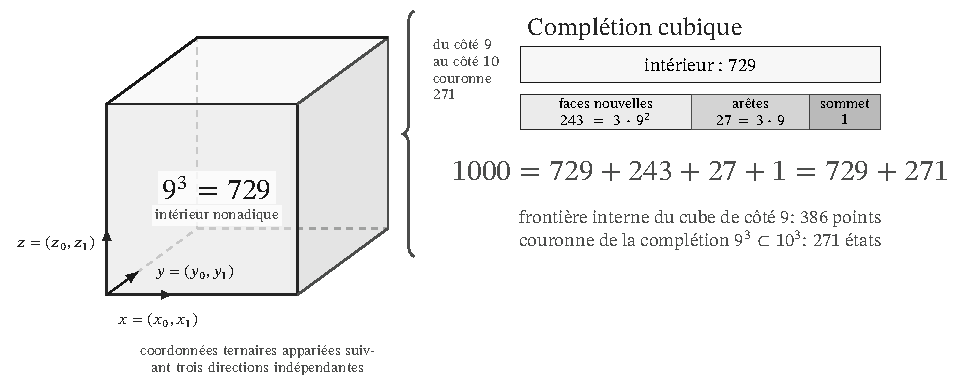
\includegraphics[width=\linewidth]{figures/cubo_emrh.pdf}
\caption{Représentation cubique de l'extension de neuf à dix classes par coordonnée. Les strates \(S_1,S_2,S_3\) placent les incidences ajoutées sur les faces, les arêtes et l'apex ; leurs cardinaux forment la couronne de \(271\) éléments. La frontière de \(386\) éléments appartient au cube initial. La perspective géométrique complète la partition de la figure ~\ref{fig:revision-emrh} ; les séparations graphiques ont une fonction schématique.}
\label{fig:completacion-cubo-recuperado}
\end{figure}


\subsubsection{Conservation de l'unité et compatibilité dimensionnelle}

La normalisation ne se limite pas à diviser une identité isolée. En dimension
\(d\), le produit \(\widehat E^d\) porte la mesure uniforme
\(\mu_d(\{x\})=10^{-d}\). La projection coordonnée
\(p_d:\widehat E^{d+1}\to\widehat E^d\) supprime la dernière coordonnée.

\begin{proposition}[Compatibilité projective des mesures normalisées]
Pour tout \(d\geq1\),
\[
 (p_d)_*\mu_{d+1}=\mu_d,
 \qquad \mu_d(\widehat E^d)=1.
\]
La masse de la strate comportant \(r\) coordonnées supplémentaires est
\(\binom dr9^{d-r}/10^d\), et la somme des masses de toutes les strates
vaut un.
\end{proposition}
\begin{proof}
Chaque point de \(\widehat E^d\) possède dix préimages. Leur masse totale est
\(10\,10^{-(d+1)}=10^{-d}\). L'égalité pour tout sous-ensemble
s'obtient en sommant sur ses points. La formule stratifiée provient
du même dénombrement que \eqref{eq:revision-estratos} ; le binôme
\((9+1)^d\) donne la normalisation totale.
\end{proof}

En dimension trois, retirer l'apex laisse une masse \(999/1000\), et
le restituer ajoute \(1/1000\). Renormaliser avant la restitution
définirait une autre mesure : la distinction est pertinente sur le plan opératoire.
En particulier, conservation de la masse probabiliste, conservation des
registres de transport et dissipation thermodynamique sont des affirmations portant sur
des objets différents. La proposition démontre la première et fournit le
support compatible pour étudier la deuxième ; la troisième requiert une
réalisation dynamique et énergétique spécifiée.

La frontière géométrique interne demeure également distincte.
Sur le représentant cartésien \(\{1,\ldots,9\}^3\), retirer
\(\{2,\ldots,8\}^3\) laisse \(386\) points. Cette frontière appartient au
cube initial, tandis que \(\widehat C\setminus C\) appartient à son
extension. La complétion cubique, le développement positionnel en base mille et
la lecture d'incidence exceptionnelle partagent des données du support ;
leurs applications respectives déterminent l'information issue de ces données qu'utilise
chaque représentation.


\subsection{Incidence cubique et réalisation lorentzienne}

La complétion cubique apporte une relation entre intérieur et frontière.
Sa géométrie peut être développée au moyen de l'incidence des six faces
avec les huit sommets. Étiquetons les faces par \((i,\varepsilon)\),
\(i\in\{1,2,3\}\), \(\varepsilon\in\{+1,-1\}\), et les sommets par
\(\nu\in\{+1,-1\}^3\). La matrice d'incidence est
\[
 M_{(i,\varepsilon),\nu}=\mathbf1_{\{\nu_i=\varepsilon\}}.
\]
Soient \(u=(1,\ldots,1)^{\mathsf T}\in\RR^6\), \(R_F\) l'opposition des faces et \(P_u=uu^{\mathsf T}/6\), \(P_-=(I-R_F)/2\).

\begin{proposition}[Quotient d'incidence de dimension quatre]
Le gramien d'incidence satisfait
\[
 MM^{\mathsf T}=12P_u+4P_-.
\]
Ses valeurs propres \(12,4,0\) ont les multiplicités \(1,3,2\).
En conséquence,
\[
 Q_\square=\RR^6/\ker(MM^{\mathsf T})
 \simeq\RR u\oplus E_-,\qquad E_-=\operatorname{im}P_-.
\]
\end{proposition}
\begin{proof}
Une face contient quatre sommets ; deux faces opposées ont une intersection vide, et deux faces distinctes non opposées partagent deux sommets. La matrice \(12P_u+4P_-\) possède précisément ces entrées. L'espace uniforme est de dimension un ; les différences entre faces opposées engendrent un espace de dimension trois, orthogonal à l'espace uniforme. Son complément est de dimension deux et appartient au noyau.
\end{proof}

La décomposition \(1+3\) procède de l'incidence. Le choix temporel
est déclaré au moyen de la forme bilinéaire
\[
 B_\square([x],[y])=\langle x,(P_--P_u)y\rangle.
\]
Elle est bien définie sur le quotient, car les deux projecteurs annulent le
noyau. Dans la base
\[
 t=[u]/\sqrt6,\qquad
 d_i=[e_{i,+}-e_{i,-}]/\sqrt2,
\]
sa matrice est \(\operatorname{diag}(-1,1,1,1)\). Sont ainsi explicités
le domaine, la décomposition et la convention de signe qui produisent
la réalisation de Minkowski. Le gramien positif détermine le quotient ;
l'affectation temporelle détermine la forme indéfinie sur celui-ci.

L'opérateur
\[
 W_\square=\sqrt6P_u+\sqrt2P_-,\qquad
 W_\square e_{i,\varepsilon}=t+\varepsilon d_i
\]
envoie les six étiquettes de face sur des directions nulles, puisque
\(B_\square(t+\varepsilon d_i,t+\varepsilon d_i)=-1+1=0\).
L'inversion d'une direction et l'opposition des faces disposent ainsi
d'une réalisation géométrique concrète.

\subsubsection{Soudure, inversion et subdivision}

La réalisation cellulaire utilise un transport inversible \(U_m(a)\),
qui conserve la forme lorentzienne, entre les fibres aux extrémités d'une
arête duale orientée \(a\), une étiquette
de face \(\lambda_m(a)\) et une orientation \(\sigma_m(a)\).
Avec \(\ell_m=\ell_0/9^m\), l'application de soudure est
\[
 \beta_m(a)=\ell_m\sigma_m(a)
 W_{\square,s(a)}e_{\lambda_m(a)}.
\]
L'inversion compatible satisfait
\[
 \beta_m(\bar a)=-U_m(a)\beta_m(a).
\]
Identifions les fibres de l'origine à deux niveaux consécutifs au moyen de l'isométrie de raffinement déclarée. Si les neuf sous-segments \(a_1,\ldots,a_9\), de niveau \(m+1\), conservent leur étiquette et leur orientation lorsqu'ils sont transportés vers cette fibre commune, alors
\begin{equation}
 \beta_m(a)=\sum_{j=1}^9
 U_{m+1}(a_1\cdots a_{j-1})^{-1}\beta_{m+1}(a_j).
 \label{eq:soldadura-refinamiento}
\end{equation}
Chaque terme transporté équivaut à \(\ell_m/9\) suivant la même
direction nulle, ce qui démontre l'identité. L'hypothèse de
compatibilité détermine quelles subdivisions réalisent ce raffinement.
L'équation réunit direction, échelle et transport, au lieu de limiter
la correspondance géométrique à un dénombrement des dimensions.

L'orientation et la forme lorentzienne étant également fixées, la dualité de Hodge dans \(\Lambda^2Q_\square^*\) satisfait \(\star^2=-I\). En dimension quatre, le signe est \((-1)^{2(4-2)+1}=-1\). On obtient une structure complexe réelle sur les deux-formes et, après complexification, les sous-espaces propres de valeurs \(+i\) et \(-i\). La réalisation électromagnétique utilisera ce domaine après la construction de la section électronique et la déclaration de son couplage.

\subsection{Compatibilité entre les réductions modulaire et positionnelle}

La base décimale par blocs intervient au moyen d'une division euclidienne
qui conserve simultanément le résidu et le quotient :
\[
 n=1000q+r,\qquad 0\le r<1000.
\]
Puisque \(1000\equiv1\pmod9\) et \(1000\equiv1\pmod3\),
\[
 n\equiv q+r\pmod9,\qquad n\equiv q+r\pmod3.
\]
Par conséquent, la réduction d'un bloc requiert la contribution du
quotient pour restituer la classe de l'entier. Les nombres \(0\) et
\(1000\) ont le même reste modulo \(1000\), mais des classes différentes
modulo \(9\) et modulo \(3\). C'est une raison opératoire de conserver
la mémoire pendant le changement de résolution.

Le raffinement ternaire et la détermination d'un préfixe décimal
peuvent se coordonner au moyen d'un unique résidu entier. Si \(N/3^L\)
est une extrémité de cylindre et \(D/1000^r\) une extrémité décimale, nous définissons
\[
 A=1000^rN-D3^L.
\]
En ajoutant six symboles ternaires, \(N'=729N+\nu\),
\(L'=L+6\), avec \(0\le\nu<729\). Si le préfixe décimal reste
fixe, on obtient
\[
 A'=729A+\nu1000^r.
\]
Si l'on incorpore en outre un bloc décimal \(\delta\), alors \(D'=1000D+\delta\), \(r'=r+1\), et
\begin{equation}
 A'=729000A+\nu1000^{r+1}-729\delta3^L.
 \label{eq:residuo-dos-bases}
\end{equation}
Les deux identités se démontrent en substituant les définitions. La
comparaison des extrémités se réduit ainsi à des opérations entières qui
retiennent la contribution de chaque prolongation. Cette compatibilité
permet de raffiner une région avant d'évaluer sa coordonnée réelle.

% Incorporación al final de extension.tex; no contiene una sección principal.
% Procedencia: RESULTADO_RECUPERADO; explicitación sectorial de las hipótesis.
% Fuentes leídas: monografía Doble proyección holográfica (cantera editorial),
% manuscrito/local/01_tesis_recuperada.tex y
% manuscrito/generated/algebra_holonomica.tex, especialmente §§1--7 y 21.
% Definición rectora de número: manuscrito/flattened/main_autosuficiente.tex,
% secciones que comienzan en líneas 22137 y 23000 de la cantera de 775 páginas.
% No se adopta su presentación global como prueba de todas las flechas TPK.

\subsection{Le nombre comme section compatible et la valeur comme lecture}
\label{hist:seccion}

La distinction entre état et observation permet de préciser quel objet est
prolongé lorsque la résolution augmente. À la profondeur \(n\), soit \(X_n\)
l'ensemble des états admissibles produits par APP--TRIT--TPK. Leurs données
comprennent position, feuillets somme et produit, résidus et quotients, régime,
orientation, retenue, phase, route, frontière, mémoire et survie. Ce ne sont pas des
coordonnées indépendantes : les évaluations arithmétiques et les transports
antérieurs imposent leurs relations. Une prolongation conserve ces relations
dans chaque antécédent, même si elle ajoute de nouvelles étapes et de nouvelles données de mémoire.
Tel est le sens de l'arithmétique des histoires formalisée ci-dessous.

Soient \(r_{m,n}:X_m\to X_n\), pour \(m\geq n\), les restrictions de
profondeur, avec \(r_{n,n}=\operatorname{id}\) et
\(r_{\ell,n}=r_{m,n}\circ r_{\ell,m}\). Chaque restriction conserve le
préfixe et l’information déjà déterminée en lui.

\begin{definition}[Section numérique compatible]
Un nombre HMT est une histoire compatible du système d’états :
\begin{equation}
 x=(x_n)_{n\geq0}\in X_\infty:=\varprojlim_n X_n,
 \qquad r_{m,n}(x_m)=x_n.
 \label{hist:limite-inverso}
\end{equation}
Un lecteur est une opération supplémentaire sur un domaine spécifié de ces
histoires. Un chiffre est une observation finie ; une valeur scalaire est une
évaluation du lecteur. Le couple formé de la section et de son lecteur constitue
une présentation munie d’une lecture, non une redéfinition de l’identité de la section.
\end{definition}

Dans le domaine archimédien \(X_\infty^{\mathrm{Arch}}\), le lecteur associe
à chaque préfixe un cylindre fermé, conserve leur emboîtement et fait tendre
leur diamètre vers zéro. Il détermine ainsi
\begin{equation}
 \operatorname{ev}_{\mathbb R}:X_\infty^{\mathrm{Arch}}\longrightarrow
 \mathbb R,\qquad
 \{\operatorname{ev}_{\mathbb R}(x)\}=\bigcap_n I_n(x).
 \label{hist:evaluacion}
\end{equation}
La construction concrète de ces cylindres et la décision de leurs frontières
sont développées dans la section~\ref{sec:generacion}. La définition
\eqref{hist:limite-inverso} n’affirme pas à elle seule que l’image de
\eqref{hist:evaluacion} soit la droite entière : une affirmation de couverture
requiert son propre théorème. Une égalité de valeurs n’établit pas non plus, sans
résultat d’injectivité, l’égalité de leurs histoires. Cette séparation
permet de parler de précision comme profondeur en conservant la différence
entre l’antécédent arithmétique et sa réalisation scalaire.

\subsection{Composition des histoires et multiplicateur de mémoire}
\label{hist:algebra}

Fixons un secteur d’états à la profondeur \(n\) et une catégorie
\(\mathcal C\) dont les flèches sont leurs histoires admissibles. La composition
s’écrit \(vu=v\circ u\) : on parcourt d’abord \(u\), puis \(v\).
Les pas élémentaires proviennent de la sélection, du transport et de
l’actualisation du TPK. Une fibre tritique locale admet l’écriture
\(\mathbb R[J_x]/(J_x^2+\tau(x)1_x)\), où
\(\tau(x)\in\{+1,0,-1\}\). Le régime et l’orientation appartiennent à
l’état transporté ; une transition entre régimes n’équivaut pas à
l’identification de leurs algèbres quadratiques.

La formulation suivante précise un secteur algébrique de cette composition.
Pour chaque objet \(x\), on se donne une algèbre réelle associative unitaire \(A_x\),
éventuellement non commutative. Pour chaque \(u:x\to y\), on se donne un
homomorphisme unital \(\rho_u:A_x\to A_y\). Nous supposons une action stricte :
\begin{equation}
 \rho_{\operatorname{id}_x}=\operatorname{id}_{A_x},\qquad
 \rho_v\rho_u=\rho_{vu}.
 \label{hist:accion-estricta}
\end{equation}
Pour chaque couple composable \(u:x\to y\), \(v:y\to z\), nous fixons un
multiplicateur central inversible
\(\Omega(v,u)\in Z(A_z)^\times\). On exige la normalisation
\(\Omega(\operatorname{id}_y,u)=\Omega(u,\operatorname{id}_x)=1_y\)
et, pour chaque triplet composable, l’identité
\begin{equation}
 \rho_w\bigl(\Omega(v,u)\bigr)\Omega(w,vu)
   =\Omega(w,v)\Omega(wv,u).
 \label{hist:cociclo}
\end{equation}
Il s’agit d’hypothèses explicites sur les transports et leurs coefficients, non d’une
conséquence du qualificatif holonomique appliqué à la dynamique. Pour appliquer cette présentation
à un secteur TPK, il faut identifier ses \(\rho_u\) et \(\Omega(v,u)\).
Les transitions exprimées par des bimodules exigent la conservation de cette
structure et ne sont pas remplacées par \eqref{hist:accion-estricta}.

L’espace des sommes finies
\[
 \mathcal H(\mathcal C,A,\rho,\Omega)
   =\bigoplus_{u\in\operatorname{Mor}(\mathcal C)} A_{t(u)}T_u
\]
est muni du produit bilinéaire
\begin{equation}
 (aT_v)(bT_u)=a\rho_v(b)\Omega(v,u)T_{vu},
 \label{hist:producto}
\end{equation}
si les flèches sont composables, et de zéro sinon. Ici, \(t(u)\)
désigne l’état terminal. La somme réunit des histoires à coefficients ; le
produit concatène les histoires en conservant le multiplicateur du registre.

\begin{proposition}[Associativité sectorielle à multiplicateur central]
Sous \eqref{hist:accion-estricta} et \eqref{hist:cociclo}, le produit
\eqref{hist:producto} est associatif. Si l’ensemble des objets est fini,
son unité est \(\sum_x1_xT_{\operatorname{id}_x}\).
\end{proposition}
\begin{proof}
Pour \(u:x\to y\), \(v:y\to z\), \(w:z\to t\), soient
\(a\in A_y\), \(b\in A_z\), \(c\in A_t\). Les deux coefficients
de \(T_{wvu}\) sont
\begin{align*}
 ((cT_w)(bT_v))(aT_u):\quad&
 c\rho_w(b)\Omega(w,v)\rho_{wv}(a)\Omega(wv,u),\\
 (cT_w)((bT_v)(aT_u)):\quad&
 c\rho_w(b)\rho_w\rho_v(a)\rho_w(\Omega(v,u))\Omega(w,vu).
\end{align*}
L’action stricte identifie \(\rho_w\rho_v(a)\) à \(\rho_{wv}(a)\).
La centralité de \(\Omega(w,v)\) permet de le déplacer à droite de
ce facteur ; \eqref{hist:cociclo} égalise alors les produits restants.
Les coefficients \(a,b,c\) ne sont pas permutés. Si le triplet n’est pas composable,
les deux parenthésages sont nuls du fait de leurs états initiaux et terminaux.
La bilinéarité achève la preuve. Les identités locales et la
normalisation de \(\Omega\) vérifient l’unité indiquée.
\end{proof}

La retenue du calendrier fournit un exemple effectif. Dans la catégorie
à un objet et de flèches \(C_9\), prenons pour coefficients
\(A=\mathbb R[z,z^{-1}]\), l’action identité et
\[
 \Omega(b,a)=z^{c_0(a,b)},\qquad
 c_0(a,b)=\left\lfloor\frac{a+b}{9}\right\rfloor,
 \quad 0\leq a,b<9.
\]
Les deux sommes de retenues d’un triplet sont
\(\lfloor(a+b+c)/9\rfloor\) ; \eqref{hist:cociclo}
est donc satisfaite. La variable formelle \(z\) enregistre le tour sans
lui attribuer de valeur numérique. Imposer ensuite \(z^{12}=1\) restitue le
registre dodécaphasique du calendrier \eqref{eq:extension108} ; conserver
\(z\) sans cette relation distingue les tours successifs. L’exemple réalise
la mémoire de ce calendrier, sans l’identifier à la totalité de la
mémoire TPK.

\subsection{Double variance du raffinement et conservation de l’unité}
\label{hist:doble-varianza}

La restriction des états prolonge les observables en sens contraire.
Considérons les algèbres de fonctions, munies du produit ponctuel,
\(D_n=\operatorname{Fun}(X_n,\mathbb R)\). La précomposition définit
\begin{equation}
 r_{m,n}^*:D_n\longrightarrow D_m,
 \qquad r_{m,n}^*f=f\circ r_{m,n}.
 \label{hist:precomposicion}
\end{equation}
Ce sont des morphismes unitaux ; ils sont également injectifs lorsque les restrictions
correspondantes sont surjectives. La limite inductive
\(D_{\mathrm{cyl}}=\varinjlim_n(D_n,r_{n+1,n}^*)\) réunit les
observations de profondeur finie. Cette algèbre n’est pas identifiée ici
à l’algèbre entière des routes : prolonger les opérateurs de transport exige
également leurs compatibilités avec le raffinement.

\begin{lemma}[Unité et naturalité de l’évaluation]
Si \(e_x\) est l’indicatrice de \(x\in X_n\), on a
\begin{equation}
 r_{m,n}^*e_x=\sum_{y:\,r_{m,n}(y)=x}e_y,
 \qquad r_{m,n}^*1_n=1_m,
 \label{hist:unidad}
\end{equation}
et, pour tous \(f\in D_n\), \(y\in X_m\),
\[
 \langle r_{m,n}^*f,y\rangle=\langle f,r_{m,n}y\rangle.
\]
Chaque section \(x\in X_\infty\) détermine une évaluation bien définie
\(D_{\mathrm{cyl}}\to\mathbb R\), donnée par \([f]\mapsto f(x_n)\)
pour \(f\in D_n\).
\end{lemma}
\begin{proof}
Les fibres de \(r_{m,n}\) forment une partition de \(X_m\). Leurs
indicatrices sont orthogonales et de somme \(1_m\), ce qui démontre
\eqref{hist:unidad}. La naturalité est la définition de la précomposition.
Enfin, \((r_{m,n}^*f)(x_m)=f(x_n)\), de sorte que deux représentants
compatibles donnent la même évaluation dans la limite inductive.
\end{proof}

L’unité globale est la fonction constante un sur toutes les possibilités ;
la section individuelle sélectionne une histoire compatible. Conserver la
première ne signifie pas immobiliser la seconde. Le raffinement peut augmenter
le nombre d’extensions et la profondeur de chaque histoire en maintenant
l’unité et toutes les évaluations de ses antécédents.

\subsection{Retour de phase, représentation de Weyl et deux lectures}
\label{hist:puente-lecturas}

La loi \eqref{eq:holonomia-memoria} acquiert une réalisation opératorielle
dans la suspension bilatérale qui sera construite dans la
section~\ref{sec:generacion}. Dans celle-ci, \(T\) est l’avancement d’un pas,
\(V_9\) observe la phase nonadique, \(W_\delta\) la phase de rotation et
\(D_M\) le degré de mémoire. En écrivant
\(\widehat\Gamma_9=T^9\) pour le tour dans cette représentation,
les relations de Weyl \eqref{eq:weyl-relojes} impliquent, sur les vecteurs
de support fini,
\begin{equation}
 \begin{aligned}
 V_9\widehat\Gamma_9&=\widehat\Gamma_9V_9,\qquad
 W_\delta\widehat\Gamma_9=e^{2\pi i9\delta}
     \widehat\Gamma_9W_\delta,\\
 [D_M,\widehat\Gamma_9]&=\widehat\Gamma_9.
 \end{aligned}
 \label{hist:tres-retornos}
\end{equation}
La première égalité découle de \(\zeta_9^9=1\) ; la deuxième, de neuf
applications de la covariance de \(W_\delta\) ; la troisième exprime
l’incrément unitaire de mémoire. La phase finie revient, tandis que la
rotation irrationnelle et la mémoire distinguent l’état suivant. Les
caractères et le paramètre \(\delta\) sont réalisés ultérieurement à partir de la
construction numérique spécifiée dans cette section : ils ne sélectionnent pas rétrospectivement
les conditions initiales. Cette représentation décrit les observables et les translations de
la suspension ; elle ne remplace ni toutes les coordonnées ni tous les opérateurs
du TPK.

La double lecture prolonge la même distinction entre histoire et observable.
Dans son domaine archimédien, on applique \eqref{hist:evaluacion} ; dans le
domaine d’incidence calibré, les applications \(Q_n\) de la
section~\ref{exc:doble-lectura} conservent les mots et les repères de
frontière. L’égalité qui y est démontrée,
\(r_{n,m}Q_n=Q_mp_{n,m}\), détermine leur prolongement \(Q_\infty\).
Sur le domaine commun aux deux lectures, on peut considérer conjointement
\(\operatorname{ev}_{\mathbb R}(x)\) et \(Q_\infty(x)\) : la
première retient la valeur ; la seconde, l’incidence transportée que son
codomaine conserve. La section précède les deux. Cette articulation permet
de passer de l’arithmétique des histoires aux constantes et à la lecture
exceptionnelle sans transformer leurs réalisations en nouvelles données initiales.


\clearpage
\section{Génération coinductive de \texorpdfstring{\(\pi,\varphi,e\)}{pi, phi, e} à profondeur arbitraire}
\label{sec:generacion}

L'émission de six blocs est une étape finie de la construction, et non un développement décimal complet. Sa fonction consiste à produire des régions munies de multiplicités, d'orientations et de règles de transport. Le prolongement doit conserver ces données et déterminer une collection compatible de préfixes de longueur arbitraire. Le mot \emph{génération} désigne cette opération ; \emph{généalogie} désigne la reconstruction de ses dépendances. Les deux notions interviennent, mais remplissent des fonctions distinctes.

\subsection{Orbites, régions et caractères de clôture, de propagation et d'auto-échelle}

Sur un mot \(w=(w_1,\ldots,w_6)\), nous définissons
\[
 r(w)=(w_3,w_1,w_2,w_5,w_6,w_4),\qquad
 s(w)=(w_4,w_5,w_6,w_1,w_2,w_3).
\]
On a \(r^3=s^2=I\) et \(srs=r^{-1}\) ; ces permutations réalisent donc le groupe diédral \(D_3\). L'action conserve le catalogue et les multiplicités et commute avec \(\Psi\). Le quotient des \(243\) mots visibles possède \(43\) orbites : trente-huit de cardinal six et cinq de cardinal trois.

La classe de clôture se reconnaît par un prédicat de fibre : ses six orientations ont cinq émissions par mot, une multiplicité totale \(1008\) et une distribution \(432+4\cdot144\). Il existe une seule orbite possédant ces propriétés dans le catalogue. Pour préciser les deux autres sélections, nous écrivons \(f(w)=\#\Psi^{-1}(w)\), \(m(w)=\sum_{U\in\Psi^{-1}(w)}\operatorname{mult}(U)\) et \(\nu(w)=(n_0,n_1,n_2)\). La classe diagonale additive d'une émission est \(d(U)=[i+j]_9\) dans les indices de zéro à huit ; sa signature additive conserve cette classe et l'orientation \(ES\) ou \(NO\). Soit \(\mathcal D(\mathcal O)\) l'ensemble de ces classes pour toutes les émissions sur une orbite.

Parmi les orbites de taille six, le prédicat conjoint
\[
 f(w)=1,\qquad m(w)=144\quad(w\in\mathcal O),\qquad
 \mathcal D(\mathcal O)=\{0,3,6\}
\]
laisse exactement six orbites. Dans ce secteur, le recensement \(\nu=(2,3,1)\), égal à celui de clôture, sélectionne uniquement la propagation ; le recensement \(\nu=(2,2,2)\) sélectionne uniquement l'auto-échelle. Le support diagonal ne peut pas être omis : sans lui, il y a quatre orbites à un seul point équilibrées de multiplicité \(144\), et non une seule. Enfin, l'existence d'une émission avec \(d=6\) et une orientation \(ES\) sélectionne un représentant de chaque orbite et conduit à
\begin{equation}
 w^{\rm cl}=010211,\qquad w^{\rm pr}=201101,\qquad w^{\rm au}=121200.
 \label{eq:palabras-regionales}
\end{equation}
Ces symboles désignent d'abord des régions du catalogue. L'identification scalaire sera démontrée au moyen de leurs lecteurs ; ils ne sont pas choisis parce qu'ils coïncident avec des chiffres d'une constante connue.

Le mot de clôture \(010211\) possède les cinq préimages suivantes :
\begin{center}\small
\begin{tabular}{@{}lll r@{}}\toprule
Émission de six blocs&Signature multiplicative&Rôle&Multiplicité\\\midrule
\(501,614,498,169,272,272\)&\(555555\)&transversal&432\\
\(810,923,870,169,272,272\)&\(339555\)&orientation positive&144\\
\(810,983,810,169,272,272\)&\(393555\)&orientation positive&144\\
\(870,923,810,169,272,272\)&\(933555\)&orientation positive&144\\
\(870,923,810,418,674,521\)&\(933717\)&retour orienté&144\\\bottomrule
\end{tabular}
\end{center}
La multiplicité \(432\) et la signature constante \(555555\) caractérisent la région transversale. Elles n'identifient pas la position centrale \((5,5)\) d'APP. Confondre une signature de six fenêtres avec une position du support éliminerait la distinction entre région numérique et structure électronique.

La microfibre possède en outre une morphologie bipartite précise. Chaque émission est un produit d'une classe de curseur additif et d'une classe multiplicative. Les trois régions positives partagent la même classe additive de dix-huit conditions ; ensemble, elles contiennent trois classes multiplicatives de huit conditions chacune. La région transversale possède un produit \(18\times24\) ; les trois positives réunies, un autre \(18\times24\) ; et le retour, un produit \(18\times8\). La décomposition par émissions comporte cinq parties, tandis que la décomposition en composantes connexes du graphe biparti en comporte trois. Toutes deux conservent les mêmes \(1008\) germes sans réduire la forme à un cardinal.

% BEGIN R27_REG01
\subsection{Incidences entre moitiés d'émissions régionales}
\label{sec:rec27-empalmes}

Soit $\mathcal U_6$ l'image des six fenêtres consécutives de l'émetteur de \ref{act21:tpk:emision}. Pour $u=(u_1,\ldots,u_6)$, nous définissons $A(u)=(u_1,u_2,u_3)$ et $B(u)=(u_4,u_5,u_6)$. Le graphe des moitiés a pour sommets ces triplets et une arête non orientée entre $A(u)$ et $B(u)$ pour chaque émission.

\begin{proposition}[Cycle des raccordements régionaux]
Les sommets
\[
\begin{aligned}
A&=(830,943,830),&B&=(109,252,252),\\
C&=(810,923,870),&D&=(169,272,272),\\
E&=(850,963,890),&F&=(149,252,212)
\end{aligned}
\]
forment le cycle $A-B-C-D-E-F-A$.
\end{proposition}
\begin{proof}
Nous écrivons chaque germe sous la forme $(i,j,d)$, avec des positions résiduelles entre
$0$ et $8$ et des directions $N=(-1,0)$, $E=(0,1)$ et $S=(1,0)$.
Les couples de germes suivants produisent, au moyen de la récurrence de
54 instants, les six émissions indiquées :
\[
\begin{array}{c|c|c}
\text{émission}&s_+&s_\times\\\hline
A\mid B&(0,6,E)&(0,6,N)\\
B\mid C&(0,6,N)&(1,5,E)\\
C\mid D&(0,6,E)&(0,1,S)\\
D\mid E&(0,6,N)&(0,4,S)\\
E\mid F&(0,6,E)&(0,3,E)\\
F\mid A&(0,6,N)&(0,1,S)
\end{array}
\]
Chaque ligne est un témoin d'appartenance à $\mathcal U_6$, obtenu par
évaluation successive des deux accumulateurs. En séparant chaque émission en
ses deux moitiés, on obtient exactement les six arêtes du cycle.
\end{proof}

Dans la classification de \eqref{eq:palabras-regionales}, \(A\mid B\), \(C\mid D\) et \(E\mid F\) produisent respectivement les mots \(w^{\rm au}\), \(w^{\rm cl}\) et \(w^{\rm pr}\). Les lecteurs régionaux identifient ensuite ces sorties à \(\varphi\), une région de \(\pi\) et \(e\). Les trois autres émissions explicitent leur raccordement dans le graphe. Le résultat décrit des incidences entre sorties de l'émetteur. La réalisation temporelle d'une incidence utilise en outre l'orientation, la phase et la mémoire de l'état enrichi. L'incorporation de l'ancrage APP et des cinq régions de $\pi$ impose des conditions de parcours supplémentaires ; le cycle précédent conserve sa fonction de témoin local de raccordement.

Le cycle de six arêtes appartient à ce graphe non orienté de
demi-émissions. Un parcours temporel enrichi conserve en outre les
données d'ancrage, d'orientation et de fermeture de sa construction. L'incidence
entre deux moitiés et le transport d'un état ont ainsi des domaines et des
conditions de composition explicites.

% END R27_REG01

% BEGIN R28_REGIONAL_CLOSURES_INPUT
% BEGIN R28_REGIONAL_CLOSURES
% Inserción después de REG01. No es un documento autónomo.
% Procedencia: U012_biografia_estructural_pi.tex, líneas 175--324.
% Testigos orientados: verificar_cierres_regionales.py; mismo problema,
% representantes distintos de los paseos impresos en U012.
% Emisor SHA-256: 42fdacab582de8e2d2cb7dfafc6204d200aef01249b3dcc37949e39507f066d8.
\subsubsection{Multigraphe de blocs et cinq clôtures régionales minimales}
\label{regcl27:seccion}

Les \(468\) émissions de l'ensemble \(\mathcal U_6\), produites par
l'émetteur APP--TRIT--TPK, déterminent un multigraphe de blocs.
L'identification de ses points d'ancrage régionaux permet de résoudre un problème
de couverture conjointe : parcourir les incidences APP, de propagation,
d'auto-échelle et de chaque région de clôture dans une même marche fermée.
Le cycle local de six raccordements de la section~\ref{sec:rec27-empalmes}
et ces couvertures conservent leurs conditions de parcours respectives.

\paragraph{Graphe de blocs et quotient exact de phase.}
Pour \(U=(U_1,\ldots,U_6)\in\mathcal U_6\), nous définissons
\begin{equation}
 A(U)=(U_1,U_2,U_3),\qquad B(U)=(U_4,U_5,U_6).
 \label{regcl27:mitades}
\end{equation}
Le multigraphe non orienté \(\widetilde G\) a pour sommets les triplets
qui apparaissent comme \(A(U)\) ou \(B(U)\), et une arête étiquetée pour chaque
\(U\), incidente à ces deux triplets. Les \(468\) étiquettes sont retenues :
deux émissions distinctes ne sont pas identifiées parce qu'elles partagent leurs extrémités, ni
parce que l'une échange les moitiés de l'autre.

La phase interne agit sur chaque triplet par rotation cyclique :
\begin{equation}
 (a,b,c)\sim(b,c,a)\sim(c,a,b),\qquad
 \operatorname{can}(a,b,c)
 =\min_{\rm lex}\{(a,b,c),(b,c,a),(c,a,b)\}.
 \label{regcl27:fase}
\end{equation}
Le graphe \(G\) remplace les extrémités de l'arête \(U\) par
\(\operatorname{can}A(U)\) et \(\operatorname{can}B(U)\), tout en conservant
son étiquette. L'équivalence agit exactement par les trois rotations
cycliques de chaque sommet ; chaque émission maintient son identité en tant qu'arête.

L'énumération du même émetteur et la recherche de composantes donnent
\begin{equation}
\begin{array}{c|r|l}
 & |V|&\text{tailles des composantes}\\ \hline
 \widetilde G&96&(28,28,28,4,4,4)\\
 G&32&(28,4)
\end{array}
\label{regcl27:componentes}
\end{equation}
Pour obtenir ces données, on réunit les extrémités distinctes, on ajoute
chaque incidence dans les deux sens et on parcourt en largeur chaque
composante non encore visitée. L'adjacence peut être dédupliquée pour compter les
composantes, mais les étiquettes parallèles sont conservées lors de la recherche de fermetures
avec des arêtes prescrites.

\paragraph{Ancrage APP et numérotation régionale.}
Les trois arêtes communes sont
\begin{equation}
\begin{aligned}
 U_{\rm APP}&=903|850|850|252|109|252,\\
 U_e&=850|963|890|149|252|212,\\
 U_\varphi&=830|943|830|109|252|252.
\end{aligned}
\label{regcl27:anclajes}
\end{equation}
Nous fixons l'extrémité \(v_{\rm APP}=\operatorname{can}A(U_{\rm APP})=850|850|903\). Dans les cinq régions déjà construites, on adopte l'ordre suivant, qui place la région transversale sur la cinquième ligne :
\begin{equation}
\begin{array}{c|l|c|r}
 i&U_\pi^{(i)}&\rho_i&m_i\\ \hline
 1&810|923|870|169|272|272&++&144\\
 2&810|983|810|169|272|272&++&144\\
 3&870|923|810|169|272|272&++&144\\
 4&870|923|810|418|674|521&--&144\\
 5&501|614|498|169|272|272&\perp&432
\end{array}
\label{regcl27:regiones}
\end{equation}
La numérotation distingue les trois régions \(++\), le retour muté
\( -- \) et la transversale \(\perp\). Ainsi,
\(\rho=(++ ,++ ,++ ,--,\perp)\) et
\(m=(144,144,144,144,432)\) dans cet ordre ; la somme reste \(1008\).

\paragraph{Cinq témoins complets avec sens de parcours.}
Dans chaque tableau, la ligne \(j\) signifie parcourir l'arête étiquetée \(e_j\) de \(v_{j-1}\) à \(v_j\). Les extrémités sont des représentants canoniques de phase. Puisque \(G\) est non orienté, la paire \((v_{j-1},v_j)\) fixe le sens de parcours de l'arête étiquetée. Chaque tableau contient exactement huit arêtes et satisfait \(v_0=v_8=v_{\rm APP}\).

La recherche en largeur décrite dans la preuve fournit les
témoins suivants, un pour chaque ensemble de quatre arêtes cibles. La
minimalité concerne la longueur ; elle admet plusieurs marches qui la réalisent.
\paragraph{Testigo \(i=1\).}
\begin{center}
\small
\begin{tabular}{rlll}
\hline
\(j\)&\(v_{j-1}\)&\(e_j\)&\(v_j\)\\
\hline
1&\(850|850|903\)&\(109|252|252|850|903|850\)&\(109|252|252\)\\
2&\(109|252|252\)&\(109|252|252|810|923|870\)&\(810|923|870\)\\
3&\(810|923|870\)&\(810|923|870|169|272|272\)&\(169|272|272\)\\
4&\(169|272|272\)&\(169|272|272|850|963|890\)&\(850|963|890\)\\
5&\(850|963|890\)&\(850|963|890|149|252|212\)&\(149|252|212\)\\
6&\(149|252|212\)&\(149|252|212|830|943|830\)&\(830|830|943\)\\
7&\(830|830|943\)&\(830|943|830|109|252|252\)&\(109|252|252\)\\
8&\(109|252|252\)&\(903|850|850|252|109|252\)&\(850|850|903\)\\
\hline
\end{tabular}
\end{center}

\paragraph{Testigo \(i=2\).}
\begin{center}
\small
\begin{tabular}{rlll}
\hline
\(j\)&\(v_{j-1}\)&\(e_j\)&\(v_j\)\\
\hline
1&\(850|850|903\)&\(169|272|272|850|903|850\)&\(169|272|272\)\\
2&\(169|272|272\)&\(169|272|272|810|983|810\)&\(810|810|983\)\\
3&\(810|810|983\)&\(810|983|810|169|272|272\)&\(169|272|272\)\\
4&\(169|272|272\)&\(169|272|272|850|963|890\)&\(850|963|890\)\\
5&\(850|963|890\)&\(850|963|890|149|252|212\)&\(149|252|212\)\\
6&\(149|252|212\)&\(149|252|212|830|943|830\)&\(830|830|943\)\\
7&\(830|830|943\)&\(830|943|830|109|252|252\)&\(109|252|252\)\\
8&\(109|252|252\)&\(903|850|850|252|109|252\)&\(850|850|903\)\\
\hline
\end{tabular}
\end{center}

\paragraph{Testigo \(i=3\).}
\begin{center}
\small
\begin{tabular}{rlll}
\hline
\(j\)&\(v_{j-1}\)&\(e_j\)&\(v_j\)\\
\hline
1&\(850|850|903\)&\(169|272|272|850|903|850\)&\(169|272|272\)\\
2&\(169|272|272\)&\(169|272|272|850|963|890\)&\(850|963|890\)\\
3&\(850|963|890\)&\(850|963|890|149|252|212\)&\(149|252|212\)\\
4&\(149|252|212\)&\(149|252|212|870|923|810\)&\(810|870|923\)\\
5&\(810|870|923\)&\(870|923|810|169|272|272\)&\(169|272|272\)\\
6&\(169|272|272\)&\(169|272|272|830|943|830\)&\(830|830|943\)\\
7&\(830|830|943\)&\(830|943|830|109|252|252\)&\(109|252|252\)\\
8&\(109|252|252\)&\(903|850|850|252|109|252\)&\(850|850|903\)\\
\hline
\end{tabular}
\end{center}

\paragraph{Testigo \(i=4\).}
\begin{center}
\small
\begin{tabular}{rlll}
\hline
\(j\)&\(v_{j-1}\)&\(e_j\)&\(v_j\)\\
\hline
1&\(850|850|903\)&\(169|272|272|850|903|850\)&\(169|272|272\)\\
2&\(169|272|272\)&\(169|272|272|850|963|890\)&\(850|963|890\)\\
3&\(850|963|890\)&\(850|963|890|149|252|212\)&\(149|252|212\)\\
4&\(149|252|212\)&\(149|252|212|870|923|810\)&\(810|870|923\)\\
5&\(810|870|923\)&\(870|923|810|418|674|521\)&\(418|674|521\)\\
6&\(418|674|521\)&\(418|674|521|830|943|830\)&\(830|830|943\)\\
7&\(830|830|943\)&\(830|943|830|109|252|252\)&\(109|252|252\)\\
8&\(109|252|252\)&\(903|850|850|252|109|252\)&\(850|850|903\)\\
\hline
\end{tabular}
\end{center}

\paragraph{Testigo \(i=5\).}
\begin{center}
\small
\begin{tabular}{rlll}
\hline
\(j\)&\(v_{j-1}\)&\(e_j\)&\(v_j\)\\
\hline
1&\(850|850|903\)&\(109|252|252|850|903|850\)&\(109|252|252\)\\
2&\(109|252|252\)&\(109|252|252|501|614|498\)&\(498|501|614\)\\
3&\(498|501|614\)&\(501|614|498|169|272|272\)&\(169|272|272\)\\
4&\(169|272|272\)&\(169|272|272|850|963|890\)&\(850|963|890\)\\
5&\(850|963|890\)&\(850|963|890|149|252|212\)&\(149|252|212\)\\
6&\(149|252|212\)&\(149|252|212|830|943|830\)&\(830|830|943\)\\
7&\(830|830|943\)&\(830|943|830|109|252|252\)&\(109|252|252\)\\
8&\(109|252|252\)&\(903|850|850|252|109|252\)&\(850|850|903\)\\
\hline
\end{tabular}
\end{center}

\begin{theorem}[Minimalité des cinq couvertures régionales]
\label{regcl27:minimalidad}
Pour chaque \(i\in\{1,\ldots,5\}\), parmi les marches fermées de \(G\)
qui parcourent au moins une fois chaque arête de
\[
 E_i^*=\{U_{\rm APP},U_e,U_\varphi,U_\pi^{(i)}\},
\]
la longueur minimale, comptée avec la multiplicité des parcours, est huit.
Les répétitions de sommets et d'arêtes sont permises.
\end{theorem}

\begin{proof}
Toute fermeture qui parcourt \(U_{\rm APP}\) passe par \(v_{\rm APP}\).
La rotation cyclique de sa liste d'étapes permet de commencer en ce sommet
sans changer ni la longueur ni la couverture. Il suffit donc de résoudre le problème
avec une origine fixe.

L'espace de recherche est l'ensemble fini
\[
 \mathscr S_i=V(G)\times\mathcal P(E_i^*),
 \qquad |\mathscr S_i|\le32\cdot16=512.
\]
L'état initial est \(s_0=(v_{\rm APP},\varnothing)\), et l'état
terminal est \(s_*=(v_{\rm APP},E_i^*)\). Lorsqu'on parcourt une arête \(e\)
incidente à \(v\), vers son autre extrémité \(v'\), on met à jour
\begin{equation}
 (v,M)\longmapsto\bigl(v',M\cup(E_i^*\cap\{e\})\bigr).
 \label{regcl27:transicion-bfs}
\end{equation}
Le masque enregistre des étiquettes d'arêtes, et pas seulement des extrémités ; c'est pourquoi des arêtes parallèles distinctes ne doivent pas être fusionnées.

Toutes les transitions coûtent une unité. Une file FIFO, initiée en
\(s_0\), extrait les états par distance croissante, marque chaque état lors de
sa première visite et garde son prédécesseur et l'étiquette parcourue.
De façon équivalente, si \(\mathcal F_0=\{s_0\}\), les nouvelles couches sont
\[
 \mathcal F_{k+1}
 =\operatorname{Succ}(\mathcal F_k)
   \setminus\bigcup_{j=0}^{k}\mathcal F_j.
\]
Par récurrence, \(\mathcal F_k\) contient exactement les états dont la distance minimale à partir de \(s_0\) est \(k\). L'énumération finie sur l'émetteur indiqué donne, pour chacune des cinq régions,
\[
 s_*\notin\bigcup_{k=0}^{7}\mathcal F_k,\qquad s_*\in\mathcal F_8,
 \qquad (\ell_1,\ell_2,\ell_3,\ell_4,\ell_5)=(8,8,8,8,8).
\]
Les tableaux présentent les cinq bornes supérieures, y compris les quatre
étiquettes requises dans chaque cas. L'exploration exhaustive des
couches précédentes prouve la borne inférieure. Leur combinaison prouve la
minimalité dans le problème déclaré.
\end{proof}

La longueur huit caractérise la couverture conjointe de quatre incidences dans chaque région de clôture. Le quotient retient les étiquettes d'émission et leurs raccordements entre classes de phase ; l'évolution temporelle enrichie conserve en outre orientation et mémoire. Cette description relie les cinq régions aux mêmes ancrages de propagation, d'auto-échelle et d'APP, et complète le cycle local de six raccordements. Le prolongement coinductif maintient ses opérateurs et ses cylindres avec ces données d'orientation et de mémoire.
% END R28_REGIONAL_CLOSURES

% END R28_REGIONAL_CLOSURES_INPUT

\subsection{Transport fini et frontière de prolongement}

Les endomorphismes \(L_0,L_1\) de l'espace des mots ternaires agissent avant la réalisation archimédienne. Leur détermination commence par les transitions de l'état arithmétique, et non par la prescription de deux matrices. Si \(U_t\) est l'étape composée de sélection, de transport et de mise à jour, le bloc observé satisfait
\[
 b_j^\chi=\Pi_6(x_j^\chi),\qquad
 x_{j+1}^\chi=U_{9j+9}\cdots U_{9j+1}(x_j^\chi),
 \qquad \chi\in\{\mathrm{cl},\mathrm{pr},\mathrm{au}\}.
\]
On forme six transitions pour chaque régime : deux consécutives dans chacune des trois régions. Les couples de matrices d'origines et de destinations obtenus dans le registre sont
\[
\begin{array}{c|c|c|c}
X_0&Y_0&X_1&Y_1\\\hline
010211&012222&010211&002111\\
012222&010211&002111&110221\\
201101&121221&102011&012222\\
121221&102011&012222&102011\\
121200&112202&121020&010210\\
112202&121020&010210&010200
\end{array}
\]
Chaque chaîne de six chiffres représente une ligne dans \(\FF_3^6\). Puisque \(\det X_0=1\) et \(\det X_1=-1\) dans \(\FF_3\), les équations \(X_aL_a=Y_a\) déterminent de manière unique \(L_a=X_a^{-1}Y_a\). Dans cette coordinatisation par vecteurs-lignes, on obtient
\[
 L_0=\begin{pmatrix}
 2&2&2&1&2&1\\2&1&2&2&1&1\\1&0&0&1&0&2\\
 0&0&1&1&1&0\\2&2&2&0&2&1\\2&1&2&1&0&0
 \end{pmatrix},\quad
 L_1=\begin{pmatrix}
 2&1&2&0&2&2\\1&2&1&1&2&0\\1&2&1&1&1&2\\
 0&1&0&0&2&1\\2&0&2&1&0&1\\0&2&2&2&1&1
 \end{pmatrix}\quad(\bmod3).
\]
Le calendrier \((L_0,L_0,L_1,L_1)\) produit quatre nouveaux blocs de six composantes. Leurs concaténations forment
\[
 w_6\longrightarrow w_{12}\longrightarrow w_{18}
 \longrightarrow w_{24}\longrightarrow w_{30}.
\]
Les sous-indices de \(w\) indiquent la longueur accumulée. La frontière \(R_{36}\) conserve la structure terminale et ouvre la relation de prolongement ; elle n'est pas renommée comme un dernier bloc périodique qui pourrait se répéter indéfiniment.

L'identité \(L=X^{-1}Y\) démontre l'unicité une fois les transitions fixées ; elle ne remplace pas la production de ces transitions par \(U_t\). La provenance de leur registre et l'examen des seize calendriers binaires sont documentés dans le supplément technique. Le calendrier indiqué est le seul de ces seize calendriers qui reproduise conjointement les trois suites de cinq blocs.

\subsection{Construction corrélée et ordre des lecteurs}
\label{gen:orden-constructor-correlacionado}

L'antécédent commun des trois régions est l'émission arithmétique avec son registre de trajectoire. APP fournit les évaluations somme et produit ; TRIT apporte la signature orientée ; la transition \eqref{eq:actualizacion} compose sélection du mode, transport cardinal et mise à jour de la mémoire. Le recensement de cette émission produit le catalogue et ses fibres. Les prédicats de multiplicité, de support diagonal et d'orientation sélectionnent les représentants de \eqref{eq:palabras-regionales}. La corrélation régionale conserve cette provenance conjointe, ainsi que les incidences et les restrictions entre ses registres.

Les transports \(L_0,L_1\) agissent sur les représentants sélectionnés
dans la coordinatisation en lignes déclarée. Le calendrier et la concaténation distinguent
la longueur du préfixe, la phase visible et la mémoire accumulée. La
coordonnée profonde et ses quotients sont explicités ci-après par
\eqref{memprof:division} et \eqref{memprof:inversa}. Les restrictions des
historiques sont conservées au sens de \ref{hist:seccion}.
La sélection orientée précise de \(R_{36}\) possède sa démonstration
d'incidence en \ref{mg01:frontera}, après la construction de \(A_W\) ;
cet emplacement conserve les antécédents utilisés dans sa preuve.

Chaque lecteur régional ajoute une opération typée au registre qu'il reçoit.
Dans la clôture, le lecteur symétrique de la pentafibre fixe la pente
primitive et la loi de composition détermine le compensateur de
\eqref{eq:lector-pi}. Dans la propagation, la composition formelle, l'unité
et le générateur orienté déterminent la récurrence
\eqref{eq:propagacion}. Dans l'auto-échelle, le calendrier des modes produit
l'incidence \eqref{eq:fav}, dont la demi-droite positive fixe la coordonnée
normalisée. Les démonstrations suivantes conservent les normalisations
et les domaines de ces trois opérations.

Les bornes rationnelles et la séparation des cylindres évaluent ensuite les caractères obtenus. L'émission positionnelle effective et sa compatibilité sont démontrées dans \ref{act21:thm:df-emision-correcta} et \ref{act21:prop:df-prefijos-compatibles}. Le registre dodécaphasique conserve sa construction propre dans \ref{act21:chap:despliegue-selector-k} ; ses coordonnées et les trois lectures régionales interviennent ultérieurement dans la clôture entière de \ref{sec:alpha}. Ainsi, sélection des régions, transport, construction des caractères et évaluation des préfixes maintiennent leurs domaines et leur ordre, au sein de la même généalogie APP--TRIT--TPK.


\subsection{Mémoire profonde et compatibilité des cylindres}
\label{memprof:seccion}

Le prolongement compare des états qui conservent simultanément restes,
quotients et frontières. Dans la coordinatisation linéaire à six coordonnées du registre,
nous prenons le représentant entier de \(L_0\) dont les entrées ont été indiquées :
\[
 A_H=\begin{pmatrix}
 2&2&2&1&2&1\\2&1&2&2&1&1\\1&0&0&1&0&2\\
 0&0&1&1&1&0\\2&2&2&0&2&1\\2&1&2&1&0&0
 \end{pmatrix},\qquad\det A_H=1.
\]
Le choix de ce représentant fait partie de la coordinatisation : la réduction
modulo trois conserve \(L_0\), tandis que le représentant entier fixe
l'opération sur les quotients profonds. Avec des vecteurs-lignes, on obtient
\begin{equation}
 \begin{aligned}
 \mathsf{Div}_H:\mathbb Z^6&\longrightarrow
       \{0,1,2\}^6\times\mathbb Z^6,\\
 x_H&\longmapsto(u_H,x_H^+),\\
 y_H&=x_HA_H,\qquad u_H=[y_H]_3,\qquad
 x_H^+=(y_H-u_H)/3 .
 \end{aligned}
 \label{memprof:division}
\end{equation}
La paire \((u_H,x_H^+)\) conserve \(y_H=u_H+3x_H^+\). Puisque \(A_H\) est unimodulaire, son inverse est entière et
\begin{equation}
 x_H=(u_H+3x_H^+)A_H^{-1}.
 \label{memprof:inversa}
\end{equation}
Cette identité récupère la coordonnée profonde à partir de son résidu et de son quotient. Les autres champs de l'état conservent leurs propres registres. L'orientation ternaire est lue ensuite au moyen de \(0\mapsto0,\ 1\mapsto+1,\ 2\mapsto-1\), en conservant le résidu \(u_H\in\{0,1,2\}^6\) et le quotient de \eqref{memprof:division}.

La coordinatisation cylindrique relie un préfixe ternaire de longueur \(L\),
d'indice entier \(N\), à \(k_{\mathrm{dec}}\) triades décimales,
d'indice \(D\). Les cylindres semi-ouverts correspondants sont
\[
 I_3(N,L)=\left[\frac N{3^L},\frac{N+1}{3^L}\right),\qquad
 I_{1000}(D,k_{\mathrm{dec}})
 =\left[\frac D{1000^{k_{\mathrm{dec}}}},
         \frac{D+1}{1000^{k_{\mathrm{dec}}}}\right).
\]
Nous définissons les entiers de frontière
\[
 a_{\mathrm{cyl}}=N1000^{k_{\mathrm{dec}}}-D3^L,\qquad
 b_{\mathrm{cyl}}=(N+1)1000^{k_{\mathrm{dec}}}-D3^L.
\]
Pour un bloc de six résidus, nous fixons son codage entier
\[
 \nu(u_H)=\sum_{j=1}^6(u_H)_j3^{6-j}
 \in\{0,\ldots,728\}.
\]

\begin{lemma}[Mise à jour entière des cylindres compatibles]
\label{memprof:cilindros}
Les cylindres précédents ont une intersection non vide si et seulement si
\(a_{\mathrm{cyl}}<3^L\) et \(b_{\mathrm{cyl}}>0\).
En ajoutant un bloc ternaire d'indice
\(\nu\in\{0,\ldots,728\}\), on a \(N'=729N+\nu\) et
\(L'=L+6\). Pour \(\Delta k_{\mathrm{dec}}\in\{0,1\}\),
les frontières sont mises à jour par
\[
 \begin{array}{ll}
 \Delta k_{\mathrm{dec}}=0:
   &a_{\mathrm{cyl}}'=729a_{\mathrm{cyl}}+\nu1000^{k_{\mathrm{dec}}},\\[2pt]
 \Delta k_{\mathrm{dec}}=1:
   &D'=1000D+\delta,\\
   &a_{\mathrm{cyl}}'=729000a_{\mathrm{cyl}}
      +\nu1000^{k_{\mathrm{dec}}+1}-\delta\,729\,3^L ,
 \end{array}
\]
où \(\delta\in\{0,\ldots,999\}\) est la triade du prolongement
compatible. Dans les deux cas,
\[
 b_{\mathrm{cyl}}'=a_{\mathrm{cyl}}'
          +1000^{k_{\mathrm{dec}}+\Delta k_{\mathrm{dec}}}.
\]
\end{lemma}
\begin{proof}
Deux intervalles semi-ouverts s'intersectent précisément lorsque chaque extrémité gauche est inférieure à l'extrémité droite de l'autre. Multiplier ces deux inégalités par \(3^L1000^{k_{\mathrm{dec}}}\) donne \(a_{\mathrm{cyl}}<3^L\) et \(b_{\mathrm{cyl}}>0\). La substitution de \(N'\), \(L'\) et \(D'\) dans
\[
 a_{\mathrm{cyl}}'
 =N'1000^{k_{\mathrm{dec}}+\Delta k_{\mathrm{dec}}}-D'3^{L'}
\]
produit les deux récurrences. Soustraire les définitions de
\(b_{\mathrm{cyl}}'\) et \(a_{\mathrm{cyl}}'\) donne la dernière identité.
\end{proof}

Ces opérations agissent sur des préfixes entiers et leurs restrictions
compatibles. La lecture archimédienne apparaît lorsqu'on évalue le système de
cylindres résultant. Le domaine de prolongement incorpore en outre
l'orientation, la retenue, la signature conjointe et les données de frontière de l'état
\(\widehat X\) de \eqref{eq:actualizacion} ; la comparaison des intervalles
est une composante de cette compatibilité conjointe.


\subsection{Cinq régions de clôture et compensation angulaire}

La région de clôture contient une composante transversale et quatre accompagnatrices. Le lecteur symétrique agit dans l'espace de leurs cinq positions au moyen de
\[
 P_5=\frac15\mathbf1\mathbf1^{\mathsf T},\qquad
 \mathbf1=(1,1,1,1,1)^{\mathsf T}.
\]
L'invariance \(P_5\lambda=\lambda\) et la conservation \(\mathbf1^{\mathsf T}\lambda=1\) imposent \(\lambda=\mathbf1/5\). Cette normalisation répartit l'unité entre les positions du lecteur ; elle ne remplace pas les multiplicités des germes \(432,144,144,144,144\) par des fréquences uniformes. La coordinatisation elliptique du lecteur réalise chaque coordonnée par \(1+\lambda_jJ\) ; sa pente est \(\lambda_j\), d'où la pente primitive \(1/5\). La règle qui fait passer d'une coordonnée normalisée à une pente est ainsi explicitée, au lieu d'identifier les deux notions sans application. Le lecteur compose les quatre positions associées selon la loi
\begin{equation}
 a\oplus b=\frac{a+b}{1-ab}.
 \label{eq:suma-pendientes}
\end{equation}
Cette loi s'obtient en multipliant \((1+aJ)(1+bJ)\) dans le régime \(J^2=-I\) et en divisant par sa composante scalaire. La composition des pentes est donc une réalisation de la structure quadratique de TRIT, et non une somme ordinaire de quatre fractions.

\begin{proposition}[Compensateur de la clôture]
La composition de quatre pentes \(1/5\) est \(120/119\). La condition de retour à une pente un détermine un unique compensateur positif de la forme \(1/q\), avec \(q>1\), et donne \(q=239\).
\end{proposition}
\begin{proof}
La première duplication donne \((1/5)\oplus(1/5)=5/12\) ; la seconde, \((5/12)\oplus(5/12)=120/119\). La condition
\[
 \frac{120/119-1/q}{1+(120/119)/q}=1
\]
équivaut à \((120-119)q=120+119\), d'où \(q=239\).
\end{proof}

Le caractère de clôture résultant a pour réalisation
\begin{equation}
 \Pi_{\rm cl}=4\left(4\arctan\frac15-\arctan\frac1{239}\right).
 \label{eq:lector-pi}
\end{equation}
L'identité angulaire de Machin reconnaît \(\Pi_{\rm cl}=\pi\). Le sens de la construction est précis : la pente et le nombre de compositions sont déclarés par le lecteur de la pentafibre ; l'équation de compensation impose \(239\). Une fois ce caractère produit, son évaluation par des séries alternées ne sélectionne pas à nouveau l'orbite des germes.

Pour \(0<x<1\), les sommes alternées
\[
 A_n(x)=\sum_{j=0}^n\frac{(-1)^jx^{2j+1}}{2j+1}
\]
encadrent \(\arctan x\) entre deux troncatures consécutives, dont la différence est \(x^{2n+3}/(2n+3)\). Appliquées aux deux pentes de \eqref{eq:lector-pi}, elles fournissent des extrémités rationnelles d'erreur explicite. La valeur numérique est ainsi calculée comme conséquence du caractère exact, sans introduire de préfixe cible.

\subsection{Lecteur de propagation et normalisation de l'unité}

La région de propagation se réalise au moyen d'une collection formelle \(P_t\in\mathcal A[[t]]\), où \(\mathcal A\) est une algèbre commutative unitaire sur \(\QQ\). Sa composition satisfait \(P_{t+s}=P_tP_s\), d'unité \(P_0=1\), et le transport élémentaire orienté fixe le générateur scalaire \(P'_0=+1\). La condition fixe son signe, et non sa seule grandeur. En écrivant
\[
 P_t=\sum_{n\ge0}a_nt^n,
\]
la normalisation détermine \(a_0=a_1=1\). La comparaison du coefficient de \(s^nt\) dans \(P_{s+t}=P_sP_t\) donne \((n+1)a_{n+1}=a_na_1\) ; de manière équivalente, \(P'_t=P_t\). Ainsi,
\begin{equation}
 (n+1)a_{n+1}=a_n,\qquad a_n=\frac1{n!}.
 \label{eq:propagacion}
\end{equation}
Le caractère en une unité de paramètre est \(\Pi_{\rm pr}=P_1\), reconnu ultérieurement comme \(e\).

La normalisation du générateur importe. La loi de semi-groupe sans cette donnée admettrait \(P_t=e^{ct}\) pour différents \(c\) ; c'est pourquoi on n'omet pas la condition qui fixe l'unité du paramètre dans le lecteur. Cette condition est antérieure à la comparaison décimale et appartient à l'exposition de la règle opératoire, et non au choix d'une valeur expérimentale.

\begin{proposition}[Bornes rationnelles de propagation]
Pour \(n\ge1\), soit \(E_n=\sum_{j=0}^n1/j!\). Alors
\[
 E_n<\Pi_{\rm pr}<E_n+\frac{n+2}{(n+1)(n+1)!}.
\]
\end{proposition}
\begin{proof}
Le premier terme omis est \(1/(n+1)!\). Chaque quotient ultérieur est au plus égal à \(1/(n+2)\). La somme géométrique majorant la queue est
\[
 \frac1{(n+1)!}\frac1{1-1/(n+2)}
 =\frac{n+2}{(n+1)(n+1)!}.
\]
L'inégalité stricte découle de la décroissance des quotients successifs.
\end{proof}

\subsection{Incidence modale et génération de l'auto-échelle}

Le sélecteur tritique produit le cycle \((+1,-1,0)\). Dans les modes \(\Sigma,\Pi\), la règle est \(+1:m\mapsto\Sigma\), \(-1:m\mapsto\Pi\), \(0:m\mapsto m\). Avec fermeture cyclique, le mode observé est \((\Sigma,\Pi,\Pi)\). Ses arêtes sont \(\Sigma\to\Pi\), \(\Pi\to\Pi\) et \(\Pi\to\Sigma\). Son incidence, dans cet ordre des modes, est donc
\begin{equation}
 F_{\rm av}=\begin{pmatrix}0&1\\1&1\end{pmatrix}.
 \label{eq:fav}
\end{equation}
Les quatre entrées s'obtiennent à partir du calendrier, et non d'une équation qui aurait préalablement reçu la valeur de \(\varphi\). La répétition du calendrier donne les dénombrements \(3F_{\rm av},9F_{\rm av},36F_{\rm av}\) aux longueurs neuf, vingt-sept et cent huit. Ces dénombrements ne sont pas les puissances de la matrice.

\begin{theorem}[Caractère positif d'auto-échelle]
L'incidence \eqref{eq:fav} possède un unique rayon propre strictement positif. En le normalisant sous la forme \((1,x)^{\mathsf T}\), sa coordonnée \(x\) satisfait \(x^2-x-1=0\), \(x>0\), et vaut \(\varphi=(1+\sqrt5)/2\).
\end{theorem}
\begin{proof}
L'équation propre donne \(x=\lambda\) et \(1+x=\lambda x\). L'élimination de \(\lambda\) produit le polynôme. Une seule de ses deux racines est positive. Comme \(F_{\rm av}^2\) a toutes ses entrées positives, le rayon positif est unique et simple. L'expression radicale reconnaît la coordonnée obtenue ; elle ne participe pas à la production de \(F_{\rm av}\).
\end{proof}

Avec \(F_0=0,F_1=1,F_{n+1}=F_n+F_{n-1}\), l'incidence induit, pour \(n\geq1\),
\[
 F_{\rm av}^n=\begin{pmatrix}F_{n-1}&F_n\\F_n&F_{n+1}\end{pmatrix}.
\]
Les quotients consécutifs \(F_{n+1}/F_n\) alternent autour de \(\varphi\). L'identité de déterminant
\[
 F_{n+1}^2-F_nF_{n+2}=(-1)^n
\]
donne une largeur exacte \(1/(F_nF_{n+1})\) entre deux quotients consécutifs. Sa croissance rend cet encadrement rationnel arbitrairement petit.

La mesure sur toutes les histoires compatibles ne coïncide pas avec la fréquence des modes du calendrier à trois événements. La fréquence chronologique est \((1/3,2/3)\). La mesure d'entropie maximale de l'enveloppe symbolique définie par \(F_{\rm av}\) se construit à partir de ses vecteurs propres et a pour rapport de poids \(\varphi^{-2}\). Cette dernière intervient dans la lecture surfacique--volumétrique ; elle ne s'obtient pas en remplaçant simplement une fréquence de comptage par une autre.

\subsubsection{Espace des trajectoires et mesure invariante entre feuillets}
\label{sec:medida-retorno-hojas}

La topologie toroïdale d'APP fixe le support des translations cardinales
et leurs classes d'enroulement. La correspondance entre feuillets procède d'
une autre opération sur ce même support : la sélection temporelle de l'
évaluation additive ou multiplicative. Son typage géométrique est
\[
 \eta_{\rm av}(\Sigma)=\mathscr H_{\rm ar},\qquad
 \eta_{\rm av}(\Pi)=\mathscr H_{\rm vol}.
\]
Le premier feuillet correspond à la lecture additive de frontière ; le second,
à la lecture multiplicative d'intérieur. Cette application transporte les étiquettes
de mode et conserve l'incidence \eqref{eq:fav}. Le carré du rapport
d'auto-échelle se détermine au moyen des trajectoires de cette incidence.

\Needspace{8\baselineskip}
\begin{definition}[Enveloppe symbolique à mémoire un]
Soit
\[
 X_{\rm av}=\{(s_k)_{k\in\mathbb Z}\in
 \{\mathscr H_{\rm ar},\mathscr H_{\rm vol}\}^{\mathbb Z}:
 (F_{\rm av})_{s_k,s_{k+1}}=1\text{ pour tout }k\}.
\]
Le décalage des indices agit sur cet espace. C'est le plus petit système
symbolique à mémoire un qui contient les suites modales et conserve
leurs couples consécutifs : il admet les deux transitions croisées et l'
auto-rétention volumétrique. La phase, l'orientation cardinale et les registres
de la trajectoire restent dans l'état TPK à partir duquel on obtient cette
enveloppe.
\end{definition}

\begin{proposition}[Pondération des trajectoires entre feuillets]
Dans l'ordre surfacique--volumétrique, la mesure invariante d'entropie maximale
de \(X_{\rm av}\) a pour matrice de transition et distribution stationnaire
\begin{equation}
 P_{\rm av}=\begin{pmatrix}0&1\\\varphi^{-2}&\varphi^{-1}\end{pmatrix},
 \qquad
 (\mu_{\rm ar},\mu_{\rm vol})
 =\frac{(1,\varphi^2)}{1+\varphi^2}.
 \label{eq:medida-hojas-exacta}
\end{equation}
En particulier, \(\mu_{\rm ar}/\mu_{\rm vol}=\varphi^{-2}\).
\end{proposition}
\begin{proof}
L'incidence déjà construite possède le vecteur propre positif \(r=(1,\varphi)^{\mathsf T}\) et la valeur propre \(\varphi\). La normalisation
\[
 (P_{\rm av})_{ij}
 =\frac{(F_{\rm av})_{ij}r_j}{\varphi r_i}
\]
donne la matrice indiquée. Ses lignes ont pour somme un par \(\varphi^{-2}+\varphi^{-1}=1\). La symétrie de \(F_{\rm av}\) implique que les poids proportionnels à \(r_i^2\) satisfont l'équilibre détaillé ; ainsi, \(\mu P_{\rm av}=\mu\). L'irréductibilité et l'auto-rétention volumique déterminent une unique distribution stationnaire.

Pour vérifier la maximalité, toute transition permise satisfait
\(\log(P_{\rm av})_{ij}=\log r_j-\log r_i-\log\varphi\).
Sous toute mesure invariante, les termes d'extrémité se compensent
en moyenne. Si \(\nu_i\) sont ses poids de sommet et
\(q_i(j)=\nu(s_1=j\mid s_0=i)\), pour \(\nu_i>0\), alors
\[
 h_\nu\leq H_\nu(s_1\mid s_0)
 =\log\varphi-\sum_{i:\nu_i>0}\nu_iD(q_i\Vert P_i)
 \leq\log\varphi,
\]
où \(D(q\Vert p)=\sum_jq_j\log(q_j/p_j)\) est l'entropie
relative sur les couples permis, et l'on adopte \(0\log0=0\).
La mesure markovienne de \eqref{eq:medida-hojas-exacta} atteint la borne.
L'égalité dans la première inégalité exige la propriété de Markov ;
l'égalité dans la seconde exige \(q_i=P_i\). La stationnarité et
l'irréductibilité fixent alors \(\mu\), ce qui établit l'
unicité. C'est la mesure de Parry de l'enveloppe définie.
\end{proof}

La fréquence \((1/3,2/3)\) compte les instants du calendrier primitif ;
\(\mu\) pondère les trajectoires de l'enveloppe. Son rapport quadratique
exprime le produit des amplitudes d'incidence d'entrée et de sortie.
La mémoire et les restrictions de phase du TPK conservent leur domaine
propre ; l'entropie de l'enveloppe correspond au système symbolique
spécifié dans cette définition.

\subsubsection{Opérateur de clôture et limite des retours marqués}
\label{sec:operador-retorno-marcado}

La coordonnée de clôture \(\pi\), générée par le lecteur régional, intervient après la construction de l'incidence modale. Soient \(e_{\rm ar}=(1,0)^{\mathsf T}\), \(e_{\rm vol}=(0,1)^{\mathsf T}\) et \(P_i=e_ie_i^{\mathsf T}\) les projecteurs de feuillet. Les conditions du lecteur sont la conservation des deux feuillets, une normalisation volumique unitaire et une marque surfacique égale à la coordonnée de clôture. Ces conditions déterminent l'opérateur positif
\begin{equation}
 D_\pi=\pi P_{\rm ar}+P_{\rm vol}
       =\begin{pmatrix}\pi&0\\0&1\end{pmatrix}.
 \label{eq:operador-marca-pi}
\end{equation}
La diagonalité exprime la conservation des feuillets et les deux entrées
expriment leurs normalisations ; l'unicité de
l'opérateur pour le lecteur fixé est ainsi explicite.

\Needspace{8\baselineskip}
\begin{proposition}[Rapport des retours de frontière]
Pour \(n\geq1\), l'évaluation marquée
\begin{equation}
 \Theta_n=
 \frac{\langle e_{\rm ar},D_\pi F_{\rm av}^{\,n}e_{\rm ar}\rangle}
 {\langle e_{\rm vol},F_{\rm av}^{\,n}e_{\rm vol}\rangle}
 =\pi\frac{F_{n-1}}{F_{n+1}}
 \label{eq:retorno-marcado-finito}
\end{equation}
satisfait
\begin{equation}
 \lim_{n\to\infty}\Theta_n
 =\pi\frac{\mu_{\rm ar}}{\mu_{\rm vol}}
 =\frac{\pi}{\varphi^2}.
 \label{eq:retorno-marcado-limite}
\end{equation}
\end{proposition}
\begin{proof}
Les entrées diagonales de \(F_{\rm av}^{\,n}\) comptent les chemins
de longueur \(n\) qui reviennent à leur feuillet initial. La formule des puissances
déjà démontrée fournit \(F_{n-1}\) et \(F_{n+1}\). L'opérateur
\(D_\pi\) multiplie par \(\pi\) le premier dénombrement. Enfin,
\(F_{n-1}/F_{n+1}\) est le produit de deux quotients consécutifs
qui convergent vers \(\varphi^{-1}\) ; sa limite est
\(\varphi^{-2}\). L'identité avec le rapport des poids découle de
\eqref{eq:medida-hojas-exacta}.
\end{proof}

L'opérateur de clôture n'apparaît qu'une seule fois, dans l'évaluation terminale du retour. Le transfert \(F_{\rm av}\) reste déterminé par le calendrier. Ainsi se compose l'information de deux lecteurs du même état : l'incidence modale détermine la pondération quadratique et la région de clôture apporte sa coordonnée à la frontière.

La composition conserve aussi le raffinement. Pour des cylindres positifs
\(I=[a,b]\) et \(J=[c,d]\), l'image du lecteur
\(\mathcal R(x,y)=x/y^2\) est l'intervalle
\[
 \mathcal Q(I,J)=\left[\frac{a}{d^2},\frac{b}{c^2}\right].
\]
La monotonie en chaque argument prouve que les cylindres emboîtés de
clôture et d'auto-échelle produisent des intervalles emboîtés du rapport ; la
positivité de leurs limites et la contraction de leurs diamètres déterminent
\(\pi/\varphi^2\). L'expression scalaire retient ainsi une chaîne
d'opérations compatible avec la profondeur, qui s'applique
ci-dessous dans ses deux orientations.

% BEGIN REV09_MULTIPLICIDAD_MODAL
\subsubsection{Multiplicité et récupération des itinéraires modaux}
\label{corpus9:modal:multiplicidad}

L'incidence \(F_{\mathrm{av}}\), construite par le calendrier tritique
dans le développement précédent, agit ici sur son enveloppe de marches
modales. Nous écrivons
\[
 F=F_{\mathrm{av}}=\begin{pmatrix}0&1\\1&1\end{pmatrix},
 \qquad 0=\Sigma,\quad 1=\Pi.
\]
La coordonnée d'auto-échelle \(\varphi\) et la demi-droite positive
\(r=(1,\varphi)\) sont les sorties déjà obtenues de cette incidence.
Sur celles-ci, on détermine la multiplicité de la lecture scalaire et
on construit une représentation réversible de chaque itinéraire.

On considère l'ensemble des marches dirigées finies
\(\gamma=(x_0,\ldots,x_n)\) de \(F\). Leurs extrémités
et leurs longueurs sont distinguées, les répétitions sont admises et les marches triviales sont incluses.
Ce domaine est l'enveloppe modale ; l'état complet du TPK
conserve en outre les registres de son histoire enrichie.
Le caractère multiplicatif prend la forme
\begin{equation}
 \chi(\gamma)=\varphi^n\frac{r_{x_0}}{r_{x_n}}
             =\varphi^{k(\gamma)},\qquad
 r=(1,\varphi),\quad k(\gamma)=n+x_0-x_n.
 \label{corpus9:modal:caracter}
\end{equation}
Les transitions \(\Sigma\to\Pi\), \(\Pi\to\Pi\) et
\(\Pi\to\Sigma\) incrémentent \(k\) de \(0\), \(1\) et \(2\),
respectivement. La première étape modifie la route tout en maintenant son
caractère. En particulier, \((1,1)\) et \((0,1,1)\) produisent tous deux
\(\varphi\) sous cette lecture.

\begin{proposition}[Multiplicité de la lecture d'auto-échelle]
\label{corpus9:modal:conteo}
Soient \(\mathcal F_k=\{\gamma:k(\gamma)=k\}\) et
\(N_k=|\mathcal F_k|\). Alors
\begin{equation}
 N_0=3,\qquad
 N_k=2\operatorname{tr}(F^k)
     =2\bigl(\varphi^k+(-\varphi^{-1})^k\bigr)
     \quad(k\geq1),
 \label{corpus9:modal:multiplicidad-exacta}
\end{equation}
et
\[
 \lim_{k\to\infty}N_k^{1/k}=\varphi.
\]
\end{proposition}

\begin{proof}
Les extrémités \(i,j\in\{0,1\}\) étant données, la longueur est déterminée par \(n=k-i+j\). Le nombre de marches ayant ces extrémités est \((F^n)_{ij}\). Pour \(k\geq1\), la somme des quatre secteurs donne
\[
 N_k=\operatorname{tr}(F^k)
      +(F^{k+1})_{01}+(F^{k-1})_{10}.
\]
L'identité \(F^2=F+I\) implique, par récurrence, que pour \(n\geq1\)
\[
 F^n=\begin{pmatrix}f_{n-1}&f_n\\f_n&f_{n+1}\end{pmatrix},
 \qquad f_0=0,\quad f_1=1,\quad f_{n+1}=f_n+f_{n-1}.
\]
Pour \(k\geq2\), les deux termes non diagonaux sont
\(f_{k+1}+f_{k-1}=\operatorname{tr}(F^k)\) ; pour \(k=1\),
leur somme est \(1+0=1=\operatorname{tr}(F)\), en utilisant \(F^0=I\).
Pour \(k=0\), les seules marches sont \((0)\), \((1)\) et \((0,1)\).
Les valeurs propres de \(F\) sont \(\varphi\) et \(-\varphi^{-1}\),
de sorte que sa trace fournit la formule fermée.
Enfin,
\[
 N_k=2\varphi^k\bigl(1+(-\varphi^{-2})^k\bigr),
\]
et le facteur entre parenthèses tend vers un ; en prenant les racines
\(k\)-ièmes, on obtient la limite.
\end{proof}

L'auto-échelle coïncide ainsi avec le taux exponentiel de croissance
des généalogies modales finies que le caractère scalaire
rend indiscernables.

\paragraph{Raffinement par composition des retours.}
Soient \(b(\gamma)\) le nombre d'arêtes \(\Pi\to\Sigma\) et \(c(\gamma)\) celui des arêtes \(\Pi\to\Pi\). Les incréments de \eqref{corpus9:modal:caracter} donnent \(k=2b+c\). Avec \(z,t\) comme indéterminées formelles, l'incidence graduée
\[
 M(z,t)=\begin{pmatrix}0&1\\tz^2&z\end{pmatrix}
\]
enregistre simultanément l'exposant et les retours. L'unique arête
de degré zéro est \(\Sigma\to\Pi\), et elle ne possède pas de cycle de degré zéro.
Chaque coefficient compte donc un ensemble fini de marches.
Si \(N_{k,b}\) désigne leur multiplicité de valeurs \(k,b\), la somme
sur toutes les longueurs satisfait
\begin{equation}
 \sum_{k,b\geq0}N_{k,b}z^kt^b
 =\mathbf1^{\mathsf T}(I-M(z,t))^{-1}\mathbf1
 =\frac{3-z+tz^2}{1-z-tz^2},
 \qquad \mathbf1=(1,1)^{\mathsf T}.
 \label{corpus9:modal:serie-graduada}
\end{equation}
En effet, l'entrée \(ij\) de \(M^n\) compte les marches de
longueur \(n\) ayant ces extrémités et leurs poids. La somme formelle
coefficient par coefficient fournit \((I-M)^{-1}\).
Le déterminant de \(I-M\) est \(1-z-tz^2\), et la somme des
quatre entrées de sa comatrice transposée est \(3-z+tz^2\).

Pour \(k\geq1\) et \(0\leq b\leq\lfloor k/2\rfloor\), il vient
\begin{equation}
 N_{k,b}=\frac{2k}{k-b}\binom{k-b}{b}.
 \label{corpus9:modal:conteo-retornos}
\end{equation}
Pour le démontrer, le développement
\[
 (1-z-tz^2)^{-1}=\sum_{m\geq0}(z+tz^2)^m
\]
donne le coefficient \(\binom{k-b}{b}\) dans \(z^kt^b\). La multiplication par le numérateur de \eqref{corpus9:modal:serie-graduada} produit
\[
 3\binom{k-b}{b}-\binom{k-b-1}{b}
   +\binom{k-b-1}{b-1}
 =2\binom{k-b}{b}+2\binom{k-b-1}{b-1}.
\]
Les coefficients hors plage sont pris égaux à zéro. Pour \(b\geq1\), l'égalité \(\binom{k-b-1}{b-1}=\frac{b}{k-b}\binom{k-b}{b}\) donne \eqref{corpus9:modal:conteo-retornos} ; pour \(b=0\), les deux membres valent deux. Le terme constant est séparé : \(N_{0,0}=3\). Pour \(k=4\), il y a quatorze marches, réparties en \(2\), \(8\) et \(4\) selon qu'elles contiennent zéro, un ou deux retours. Le même caractère admet donc des compositions internes distinctes.

\begin{proposition}[Récupération réversible et transport des codes]
\label{corpus9:modal:recuperador}
Chaque marche de l'enveloppe modale admet un code
\[
 \mathcal C(\gamma)=(k,a),\qquad 0\leq a<N_k,
\]
avec un décodage \(\mathcal D\) tel que
\[
 \mathcal D\mathcal C=\mathrm{id},\qquad
 \mathcal C\mathcal D=\mathrm{id}.
\]
Si \(A_v(\gamma)=\gamma v\) prolonge par une arête admissible et
\(T\) supprime le dernier état d'une marche de longueur positive,
leurs représentations
\[
 \mathcal E_v=\mathcal C A_v\mathcal D,\qquad
 \widehat T=\mathcal C T\mathcal D
\]
satisfont, dans leurs domaines respectifs,
\begin{equation}
 \widehat T\mathcal E_v=\mathrm{id},\qquad
 k(A_v\gamma)-k(\gamma)=1+x_n-v.
 \label{corpus9:modal:transporte-codigos}
\end{equation}
\end{proposition}

\begin{proof}
Pour chaque \(k\), on ordonne les secteurs non vides selon \((n,i,j)\)
et, au sein de chaque secteur, les marches dans l'ordre lexicographique de leurs
états. Le nombre de continuations de longueur \(m\) de
\(v\) à \(j\) est \((F^m)_{vj}\). En parcourant une marche, on additionne
les tailles des secteurs précédents et, à chaque position, celles
des continuations lexicographiquement antérieures à celle choisie.
Le résultat est son indice \(a\), compté à partir de zéro.

Pour inverser le processus, on soustrait de l'indice la taille de chaque
secteur précédent jusqu'à localiser l'unique secteur qui le contient.
À chaque position, on procède de même avec les tailles des
continuations. Ces ensembles forment une partition disjointe
et exhaustive du secteur de départ. Pour la longueur zéro, l'unique
marche d'un secteur non vide est son sommet. En supposant récupérées
les continuations de longueur \(m-1\), les intervalles d'indices
de chaque premier successeur identifient de manière univoque ce successeur et l'
indice restant de sa continuation. La récurrence sur \(m\) prouve
que les deux procédures sont inverses, aussi bien sur les marches que
sur les indices \(0,\ldots,N_k-1\).

L'ordre lexicographique sérialise la route existante ; les opérations qui génèrent la route précèdent cette sérialisation. Puisque \(T A_v=\mathrm{id}\), les deux identités inverses donnent
\[
 \widehat T\mathcal E_v
 =\mathcal C T\mathcal D\mathcal C A_v\mathcal D
 =\mathcal C T A_v\mathcal D
 =\mathrm{id}.
\]
Enfin, la définition de l'exposant donne
\[
 k(A_v\gamma)=(n+1)+x_0-v,\qquad
 k(\gamma)=n+x_0-x_n,
\]
dont la différence est la deuxième identité.
\end{proof}

\paragraph{Capacité de distinction avec exposant connu.}
Lorsque \(k\) est connu, une représentation binaire injective de longueur
fixe \(\ell\) exige \(2^\ell\geq N_k\), par le principe des
tiroirs. Par conséquent,
\(\ell\geq\lceil\log_2N_k\rceil\).
L'indice \(a\) précédent atteint cette longueur au moyen de sa
représentation binaire, complétée de zéros initiaux si
nécessaire. Ce minimum correspond à la transmission de l'indice
avec \(k\) connu ; la transmission de \(k\) et la délimitation des
codes de longueur variable ont leurs propres coûts. De plus,
\[
 \lim_{k\to\infty}\frac{\log_2N_k}{k}=\log_2\varphi.
\]
L'égalité mesure la capacité combinatoire de distinction des routes dans l'enveloppe modale.

\paragraph{Information de fibre sous une distribution explicite.}
\(k\) étant fixé, soit \(R_k\) une marche choisie uniformément dans \(\mathcal F_k\). Nous utilisons les logarithmes naturels et \(H(R_k)=-\sum_{\gamma\in\mathcal F_k}p_\gamma\log p_\gamma\), avec \(p_\gamma=1/N_k\). Toutes ces marches ont pour caractère \(\varphi^k\), de sorte que
\[
 H(R_k\mid\chi(R_k))=\log N_k,\qquad
 H(R_k\mid\mathcal C(R_k))=0.
\]
La première égalité provient du fait que la lecture est constante sur la fibre ; la seconde, du décodage unique déjà démontré. En particulier, \(\log N_k/k\to\log\varphi\).

Pour \(k=4\), le caractère laisse une incertitude de \(\log14\)
nats. Les trois classes \(B=b(R_4)\) ont les probabilités
\(2/14\), \(8/14\) et \(4/14\). Conditionnée à chaque classe, la
distribution reste uniforme sur ses \(2\), \(8\) ou \(4\)
éléments, respectivement. Par définition de l'entropie
conditionnelle,
\[
 H(R_4\mid B)
 =\frac2{14}\log2+\frac8{14}\log8+\frac4{14}\log4.
\]
L'indice au sein de la classe, conjointement avec \(B\), retrouve univoquement
la marche. Ces valeurs appartiennent à la distribution uniforme
de la fibre modale déclarée. La mesure de l'espace complet des
histoires, la réalisation temporelle de \(k\) et toute lecture
thermique conservent leurs domaines et transducteurs respectifs.
% END REV09_MULTIPLICIDAD_MODAL


Une fois les caractères générés, les deux orientations du lecteur
\[
 R(x,y)=\frac{x}{y^2}
\]
fournissent
\begin{equation}
 \rho_A=\frac\pi{\varphi^2},\qquad
 \rho_E=\frac\varphi{\pi^2},\qquad
 \varphi^3\rho_A^2\rho_E=1.
 \label{eq:areal-electron}
\end{equation}
La seconde expression apparaîtra dans l'exposant électronique. La première s'obtient également comme limite de la lecture marquée \(\pi F_{n-1}/F_{n+1}\). L'échange des arguments les relie, mais ne transforme pas un reparamétrage de l'équation électronique en une deuxième dérivation indépendante de tous ses coefficients.

% Articulación posterior a la generación de pi, phi y e.
% Contenido acumulativo; no reemplaza el desarrollo previo del TRIT.
\subsection{Réalisations exponentielles des coordonnées générées}
\label{euler-trit-articulacion}

Les coordonnées régionales déjà déterminées permettent de reconnaître les
réalisations concrètes de la collection quadratique du TRIT. L'ordre est
essentiel : la construction des régions précède l'évaluation d'une
exponentielle aux paramètres \(\pi\) ou \(2\log\varphi\). Ces expressions
identifient la fonction des coordonnées dans des opérateurs construits à partir
d'APP et du TPK ; elles n'interviennent pas dans la sélection des préfixes qui les produisent.

\subsubsection{Cycle ternaire, transport nilpotent et incidence des feuillets}

La multiplication \(a(r)=4r\) dans \(\mathbb Z/9\mathbb Z\) est d’ordre
\(3\). Sur les unités, elle détermine les orbites \(\{1,4,7\}\) et
\(\{2,8,5\}\). Dans le module d’augmentation de l’une quelconque d’entre elles, formé
des combinaisons entières dont les coefficients ont une somme nulle, la base
\((e_r-e_{4r},e_{4r}-e_{7r})\) donne
\[
 C=\begin{pmatrix}0&-1\\1&-1\end{pmatrix},
 \qquad C^2+C+I=0.
\]
La forme restreinte a pour matrice de Gram
\(\bigl(\begin{smallmatrix}2&-1\\-1&2\end{smallmatrix}\bigr)\).
Dans les évaluations résiduelles modulo \(9\), l’action distingue les feuillets :
\(S(ax,ay)=aS(x,y)\), tandis que \(P(ax,ay)=a^{-1}P(x,y)\).
La réalisation cyclique conserve donc une orientation contragrédiente
entre somme et produit. Les quotients du relèvement entier sont conservés
dans le registre arithmétique correspondant.

Le transport parabolique élémentaire est représenté par
\[
 N=\begin{pmatrix}0&1\\0&0\end{pmatrix}.
\]
L’incidence surfacique--volumique déjà construite dans \eqref{eq:fav} fournit
\[
 F_{\rm av}=\begin{pmatrix}0&1\\1&1\end{pmatrix},
 \qquad A=F_{\rm av}^2=\begin{pmatrix}1&1\\1&2\end{pmatrix}.
\]
Les trois opérateurs agissent dans des espaces réels déclarés : le module
d’augmentation tensorisé avec \(\mathbb R\), le plan du transport nilpotent et
le plan d’incidence modale. Le partage d’une dimension matricielle n’identifie
ni ces espaces ni leurs coordonnées.

\begin{proposition}[Générateurs concrets des trois types]
\label{euler-trit-generadores}
Les opérateurs
\[
 J_{\mathrm e}=\frac{2C+I}{\sqrt3},\qquad
 J_{\mathrm p}=N,\qquad
 J_{\mathrm h}=\frac{2A-3I}{\sqrt5}
\]
satisfont, respectivement,
\[
 J_{\mathrm e}^{\,2}=-I,\qquad
 J_{\mathrm p}^{\,2}=0,\qquad
 J_{\mathrm h}^{\,2}=I.
\]
\end{proposition}
\begin{proof}
La relation de \(C\) implique \((2C+I)^2=-3I\).
La multiplication directe donne \(N^2=0\).
Enfin, \(A\) est de trace \(3\) et de déterminant \(1\), d’où
\(A^2-3A+I=0\) et \((2A-3I)^2=5I\).
\end{proof}

\begin{proposition}[Trois évaluations de l’identité exponentielle]
\label{euler-trit-evaluaciones}
Dans les réalisations précédentes,
\begin{equation}
 \boxed{
 \exp(\pi J_{\mathrm e})+I=0,\qquad
 \exp(J_{\mathrm p})=I+J_{\mathrm p},\qquad
 \exp(2\log\varphi\,J_{\mathrm h})=F_{\rm av}^{\,2}.}
 \label{euler-trit-tres-evaluaciones}
\end{equation}
\end{proposition}
\begin{proof}
La spécialisation elliptique de l’exponentielle tritique donne
\(\cos\pi\,I+\sin\pi\,J_{\mathrm e}=-I\).
La nilpotence élimine exactement les termes de degré au moins \(2\)
dans la deuxième expression. Pour la troisième, \(\varphi^2=\varphi+1\) implique
\[
 \cosh(2\log\varphi)=\frac32,\qquad
 \sinh(2\log\varphi)=\frac{\sqrt5}{2}.
\]
L’exponentielle vaut donc
\(\frac32I+\frac{\sqrt5}{2}J_{\mathrm h}=A\).
\end{proof}

La première égalité représente le demi-tour elliptique ; le tour complet
satisfait \(\exp(2\pi J_{\mathrm e})=I\). La deuxième maintient un terme
linéaire non nul : le régime parabolique exprime un transport, et non une absence
d'évolution. La troisième réalise une avancée hyperbolique unimodulaire. Ses
valeurs propres sont \(\varphi^2\) et \(\varphi^{-2}\) ; une direction se dilate et
l'autre se contracte en conservant le déterminant. Les trois évaluations
emploient des paramètres distincts d'une collection exponentielle commune.

Dans cette collection, \(e\) intervient par l'évaluation scalaire
\(\exp(I)=eI\) et la loi \(\exp(sI)\exp(tI)=\exp((s+t)I)\).
Son rôle ne se limite pas au type parabolique. La coordonnée \(e\), obtenue
auparavant à partir de sa région, est reconnue ici comme l'évaluation en l'unité
de l'exponentielle ; cette identité ne remplace pas sa généalogie coinductive.

\subsubsection{Résolution polynomiale des régimes}

Les trois réalisations admettent une présentation compacte sur la somme
directe de leurs espaces. On définit
\[
 \mathbb J=J_{\mathrm e}\oplus J_{\mathrm p}\oplus J_{\mathrm h},
 \qquad Q=\mathbb J^2.
\]
Les relations précédentes impliquent
\[
 \mathbb J^6=\mathbb J^2,\qquad Q^3=Q.
\]
L’emploi de \(Q\) maintient ce carré opératoriel distinct du registre
dodécaphasique \(K\).

\begin{proposition}[Projecteurs polynomiaux de régime]
\label{euler-trit-proyectores}
Les applications
\[
 p_{\mathrm e}=\frac{Q^2-Q}{2},\qquad
 p_{\mathrm p}=I-Q^2,\qquad
 p_{\mathrm h}=\frac{Q^2+Q}{2}
\]
sont des idempotents mutuellement orthogonaux, de somme \(I\), qui restituent les trois
termes de la somme directe représentant les régimes.
\end{proposition}
\begin{proof}
Les trois polynômes prennent les valeurs \((1,0,0)\), \((0,1,0)\) et
\((0,0,1)\) aux points \(-1,0,+1\), respectivement. Les différences
entre leurs carrés et eux-mêmes, ainsi que leurs produits croisés, sont
des multiples de \(X^3-X\). Substituer \(Q\), qui annule ce polynôme, démontre
les identités. Dans les trois blocs, \(Q\) agit comme \(-I,0,I\).
\end{proof}

On obtient ainsi
\begin{align}
 \exp(t\mathbb J)
 ={}&p_{\mathrm e}(\cos t\,I+\sin t\,\mathbb J)
   +p_{\mathrm p}(I+t\mathbb J)\notag\\
   &+p_{\mathrm h}(\cosh t\,I+\sinh t\,\mathbb J).
 \label{euler-trit-exponencial-total}
\end{align}
Chaque terme conserve sa relation quadratique et la conjugaison inverse
son évolution. La représentation totale réunit les trois régimes, mais ne
définit pas à elle seule un opérateur de transition entre eux. Une telle transition
requiert les applications de transport du TPK avec leurs domaines, leur orientation et
leur mémoire. L’articulation exponentielle permet de reconnaître leurs types sans
remplacer cette dynamique par une identification des fibres.

% PROCEDENCIA FOCAL (no impresa)
% Resultado recuperado: tres generadores y tres evaluaciones exponenciales.
% Propietario completo:
% BASE/manuscrito/sections/hmt/09b_algebras_cuadraticas.tex:289-516.
% Antecedente causal de C y acción contragrediente:
% BASE/manuscrito/sections/hmt/03d_esqueleto_ciclotomico_app.tex:13-47,145-246.
% Los tres tipos y la orientación están en:
% BASE/manuscrito/sections/hmt/02_trit_geometrias.tex:83-196.
% Resolución polinómica recuperada:
% output/INVESTIGACION_HOLONOMIA_NONADICA_CRISTAL_APERIODICO_20260903/
% ALGEBRA_HOLONOMICA_UNIVERSAL_Y_EULER_TRITICO.md, secciones 8-11 y 22.
% Los cuatro propietarios se leyeron completos. BASE designa:
% /Users/ruben/Documents/HMT2/
% EL_CIERRE_HOLOGRAFICO_DEL_INFINITO_SUCESOR_102_CAPITULOS_2026-08-28_EN_TRABAJO/
% No se incorpora la identidad P9(alpha)=delta del documento especializado:
% esa identificación no pertenece a este bloque.
% Tampoco se identifica una dirección nilpotente con la vacancia electrónica,
% ni se presume una representación global del transporte por la suma directa.
% COMPROBACIONES: Python estándar, enteros y Fraction.
% C^2+C+I=0; (2C+I)^2=-3I; N^2=0; (2Fav^2-3I)^2=5I.
% 81 pares de residuos verifican las dos acciones contragredientes.
% Los 3 proyectores se verificaron en Q=-1,0,+1; prueba general en texto.
% 6 labels únicos y entornos equilibrados. Sin compilación.


\subsection{Cylindres compatibles et profondeur arbitraire}

La réalisation d'un bloc ternaire \(b=(b_1,\ldots,b_6)\) est l'entier
\[
 \nu(b)=\sum_{j=1}^6b_j3^{6-j}\in\{0,\ldots,728\}.
\]
Une suite de blocs définit des préfixes entiers par \(N_{n+1}=729N_n+\nu(b_{n+1})\), en commençant en \(N_0=m\), où \(m\) est la partie entière déterminée par le lecteur. Les fourchettes précédentes situent les caractères de clôture, de propagation et d'auto-échelle dans \((3,4)\), \((2,3)\) et \((1,2)\), respectivement ; leurs valeurs initiales sont donc \(m=3,2,1\). Les blocs suivants raffinent la partie fractionnaire. Le cylindre correspondant est
\begin{equation}
 I_n=\left[\frac{N_n}{729^n},\frac{N_n+1}{729^n}\right],
 \qquad |I_n|=729^{-n}.
 \label{eq:cilindro}
\end{equation}
La convention semi-ouverte est utilisée pour sélectionner un représentant lorsqu'une valeur tombe sur une frontière. Pour le passage à la limite, on utilise les fermetures de ces intervalles et on identifie les deux développements de frontière équivalents. Cette précision empêche de supposer que toute intersection d'intervalles semi-ouverts emboîtés est automatiquement non vide.

\begin{theorem}[Détermination de la réalisation scalaire]
Une histoire de blocs compatible détermine une unique limite des extrémités gauches de \eqref{eq:cilindro}. Si un caractère exact dispose d'encadrements rationnels de largeur arbitrairement petite et se sépare de la frontière de chaque cylindre décimal examiné, chaque préfixe décimal de longueur finie est déterminé après un calcul fini. Les préfixes ainsi obtenus sont compatibles entre eux.
\end{theorem}
\begin{proof}
L'extension d'un bloc conserve le préfixe précédent par division euclidienne. Les cylindres fermés sont emboîtés et leur diamètre tend vers zéro ; leurs extrémités gauches forment une suite de Cauchy et possèdent une unique limite. Pour une longueur décimale fixée, une valeur séparée des frontières de la partition possède une distance positive à celles-ci. Une fourchette suffisamment étroite est contenue dans une unique cellule et détermine son préfixe. L'unicité de la cellule et l'emboîtement des partitions prouvent la compatibilité par troncature. Aux points à développement terminal, il faut ajouter la décision exacte de frontière et sa convention de représentation ; cette décision ne se déduit pas d'une largeur numérique seule.
\end{proof}

\begin{corollary}[Obtention finie et compatibilité des préfixes régionaux]
\label{gen:prefijos-regionales}
Pour chacune des réalisations \(\pi,\varphi,e\) et pour toute longueur
décimale finie, les encadrements construits déterminent le préfixe correspondant
par un calcul fini. Les préfixes obtenus à différentes profondeurs
sont compatibles par troncature.
\end{corollary}
\begin{proof}
Les caractères de clôture, de propagation et d'auto-échelle possèdent les encadrements précédents. Après leur reconnaissance, l'irrationalité de \(\pi,e,\varphi\) garantit leur séparation des frontières rationnelles de chaque partition décimale finie. On applique le théorème précédent à chaque caractère.
\end{proof}
La profondeur arbitraire exprime le quantificateur du corollaire : pour tout
horizon fini, il existe un calcul qui détermine son préfixe. L'objet
mathématique est la collection compatible complète ; chaque exécution en obtient une
projection finie.

\subsection{Involution spéculaire et synchronisation des régions}

La connexion nonadique transporte conjointement les trois caractères. Dans la coordinatisation de la neuvième phase, l'axe d'auto-échelle et la somme ternaire de clôture et de propagation restent fixés sous l'échange spéculaire. L'inversion hélicoïdale change le sens du transport ; la réflexion des deux canaux change leur orientation relative. Ce sont des involutions différentes, bien qu'elles agissent sur le même système de trajectoires.

Les coïncidences de recensement illustrent cette coordination :
\begin{center}
\begin{tabular}{@{}c rrr l@{}}\toprule
Phase&\(N_\pi\)&\(N_e\)&\(N_\varphi\)&Égalité des dénombrements\\\midrule
4&207&207&122&\(N_\pi=N_e\)\\
5&39&151&151&\(N_e=N_\varphi\)\\
6&110&110&69&\(N_\pi=N_e\)\\
7&81&29&81&\(N_\varphi=N_\pi\)\\
8&59&59&59&synchronisation triple\\
9&43&43&43&synchronisation triple\\\bottomrule
\end{tabular}
\end{center}
Ces entiers comptent des coordonnées compatibles des régions. Ils n'affirment pas une égalité entre \(\pi\), \(e\) et \(\varphi\) en tant que nombres réels. Si
\[
 \partial(a,b,c)=(a-b,b-c,c-a),
\]
son image appartient au réseau \(A_2=\{(u,v,w)\in\ZZ^3:u+v+w=0\}\). Aux phases huit et neuf, la composante relative s'annule, mais la composante diagonale passe de \((59,59,59)\) à \((43,43,43)\). La synchronisation relative coexiste avec un déplacement de \(-16\) par canal. La fermeture qui conduira à \(\alpha\) doit conserver les deux informations : coïncidence relative et évolution de la mémoire.

\subsection{Suspension hélicoïdale sturmienne}

La relation entre les bases neuf et dix de la complétion définit le paramètre adimensionnel
\begin{equation}
 \delta=\frac{\log(10/9)}{\log10}.
 \label{eq:delta-sturm}
\end{equation}
Elle ne s'obtient pas à partir d'une constante physique cible. C'est l'échelle logarithmique relative de deux bases déjà présentes dans la construction. Son emploi comme lecture symbolique du raffinement a une conséquence exacte.

\begin{lemma}[Irrationalité de la pente]
Le nombre \(\delta\) est irrationnel.
\end{lemma}
\begin{proof}
Si \(\delta=p/q\), \(q>0\), alors \((10/9)^q=10^p\) et \(9^q=10^{q-p}\). La factorisation du premier membre contient le nombre premier trois et celle du second uniquement les nombres premiers deux et cinq. L'égalité est impossible.
\end{proof}

Le mot mécanique inférieur, d'ordonnée à l'origine \(\theta\), est
\[
 z_n(\theta)=\lfloor(n+1)\delta+\theta\rfloor-\lfloor n\delta+\theta\rfloor\in\{0,1\}.
\]
On l'obtient en observant la rotation \(\theta\mapsto\theta+\delta\pmod1\) au moyen de l'intervalle \([1-\delta,1)\). La suite d'événements a pour densité \(\delta\), et la somme sur toute fenêtre de longueur \(L\) vaut \(\lfloor L\delta\rfloor\) ou \(\lceil L\delta\rceil\). Puisque \(21<1/\delta<22\), les séparations entre événements sont vingt et un ou vingt-deux. Le mot qui indique quels sont les intervalles courts est un autre mot mécanique de pente \(\sigma=22-1/\delta\) ; ses événements sont séparés par six ou sept intervalles primaires. La seconde échelle est induite par la première et n'est pas un second paramètre libre.

% Desarrollo reunido de DESARROLLO_MATEMATICO, apartados 38--40 y 50.
\subsubsection{Indice de capacité, lacunes et induction du régime tritique}
\label{vac-capacidad-trit}

La suite des lacunes est liée au raffinement par une
identité d'incréments. Pour la montrer, on fixe l'origine de phase
\(\theta=0\). Soient
\[
 \rho=\log_{10}9=1-\delta,\qquad
 \mathcal C_t=\lfloor(t+1)\rho\rfloor\quad(t\geq0).
\]
L'indice \(\mathcal C_t\) exprime la capacité décimale du raffinement
dans la normalisation qui compare un bloc ternaire de \(6\) positions,
avec \(729\) possibilités, et un bloc décimal de \(3\) positions, avec
\(1000\) possibilités. En effet,
\(\log_{1000}729=\log_{10}9=\rho\). La lettre \(K\) est réservée au
registre dodécaphasique qui sera construit ultérieurement.

\begin{proposition}[Complémentarité de la capacité et de la lacune]
\label{prop:capacidad-vacancia}
Pour \(t\geq1\),
\begin{equation}
 \mathcal C_t-\mathcal C_{t-1}=1-z_t(0).
 \label{eq:capacidad-vacancia}
\end{equation}
Par conséquent, si \(0\leq a<b\),
\[
 \mathcal C_b-\mathcal C_a+
 \sum_{t=a+1}^{b}z_t(0)=b-a.
\]
\end{proposition}
\begin{proof}
L'irrationalité de \(\delta\) donne
\[
 \mathcal C_t
 =t+1-\lceil(t+1)\delta\rceil
 =t-\lfloor(t+1)\delta\rfloor.
\]
La soustraction de deux termes consécutifs produit
\eqref{eq:capacidad-vacancia}. La somme sur l'intervalle est télescopique.
\end{proof}

Chaque transition augmente d'une unité le compteur des blocs. Si
\(z_t=0\), la capacité augmente également ; si \(z_t=1\), la capacité se
maintient tandis qu'une transition est incorporée à l'histoire. La lacune
est ici un événement de rétention de capacité, de position et
d'antécédent déterminés. Le bilan précédent conserve exactement la
longueur entre capacité acquise et lacunes enregistrées. La phase
observée \(g_t^{\rm cap}=[\mathcal C_t]_9\) vérifie
\[
 g_t^{\rm cap}-g_{t-1}^{\rm cap}\equiv1-z_t\pmod9.
\]
Cette phase de capacité et la phase chronologique \([t]_9\) sont deux
observations différentes. Une rétention locale de capacité et un tour
complet de l'holonomie ont des mécanismes distincts, bien que les deux
permettent de conserver l'observation de phase avec modification de l'état.

La relation avec TRIT peut se suivre dans les positions mêmes des lacunes.
Pour \(j\geq1\), définissons
\[
 p_j=\left\lfloor\frac j\delta\right\rfloor,\qquad
 v_j=\mathcal C_{p_j},\qquad h_j=p_{j+1}-p_j.
\]
L'inégalité \(p_j\delta<j<(p_j+1)\delta\) identifie \(p_j\)
comme la position de l'événement \(j\). Comme \(0<\delta<1\), elle donne aussi
\(\lfloor(p_j+1)\delta\rfloor=j\), et par conséquent
\[
 v_j=p_j-j,\qquad
 v_{j+1}-v_j=h_j-1.
\]
Si \(s_j=22-h_j\), alors \(s_j\in\{0,1\}\) et
\begin{equation}
 [v_{j+1}]_3=[v_j-s_j]_3.
 \label{eq:vacancia-regimen}
\end{equation}
Un intervalle de longueur \(22\) conserve la classe ; un intervalle de longueur
\(21\) la décale d'une unité dans le sens négatif. Le sélecteur canonique
s'applique à la phase positive \(r_j=1+[v_j]_9\) :
\[
 \tau_j=M_{\rm ph}(r_j).
\]
Un régime tritique est ainsi déterminé par l'indice de capacité
retenu à chaque événement, en plus du codage binaire de la lacune.

Les positions des intervalles courts forment le codage mécanique
induit de pente \(22-1/\delta\). Leurs espacements \(6\) et \(7\)
déterminent les longueurs des plateaux de la classe \([v_j]_3\), une
fois l'origine et la convention des extrémités fixées. Les premières classes
sont \(2\) pendant \(6\) événements, \(1\) pendant \(7\) et \(0\) pendant
\(7\) ; le premier segment de \(6\) est la restriction initiale d'un plateau.
Leurs signatures parcourent \(0,-1,+1\). Les équations
\eqref{eq:capacidad-vacancia} et \eqref{eq:vacancia-regimen} explicitent le
lien entre raffinement, lacunes et sélection du régime. La lecture
quadratique de TRIT réalise ensuite ces types au moyen de leurs générateurs
respectifs ; l'événement temporel et sa représentation géométrique
conservent ainsi une dépendance identifiable.

L'inversion de l'indice monotone fournit une autre observation utile :
\[
 \mathcal T(k)=\min\{t:\mathcal C_t=k\}
   =\left\lceil\frac k\rho\right\rceil-1\qquad(k\geq1).
\]
Si \(\sigma=\rho^{-1}-1\), le nombre de blocs nécessaires pour acquérir
\(m\) unités de capacité est
\[
 \mathcal T(k+m)-\mathcal T(k)
 =m+\lceil(k+m)\sigma\rceil-\lceil k\sigma\rceil
 \in\{m+\lfloor m\sigma\rfloor,m+\lceil m\sigma\rceil\}.
\]
En particulier, \(9\) unités de capacité nécessitent \(9\) ou \(10\)
blocs. La période d'une phase finie reste exacte, tandis que le
temps de retour mesuré par l'autre indice admet deux valeurs. Cette
distinction fait partie de la dynamique du raffinement et ne constitue pas une correction
de ses valeurs numériques a posteriori.


\begin{theorem}[Complexité des lectures de phase]
Pour \(m\ge1\), le mot mécanique a une complexité factorielle \(p(m)=m+1\). En conservant la phase \(n\bmod9\), la complexité est \(p_9(m)=9(m+1)\) ; en conservant seulement sa classe ternaire, elle est \(p_3(m)=3(m+1)\). Les trois entropies topologiques sont nulles.
\end{theorem}
\begin{proof}
Les prédécesseurs des deux extrémités de l'intervalle de codage forment, pour les facteurs de longueur \(m\), \(m+1\) points distincts du cercle : la coïncidence entre extrémités translatées élimine les doublons et l'irrationalité empêche toute coïncidence supplémentaire. Ces points déterminent \(m+1\) intervalles à itinéraires constants et distincts. Toute orbite irrationnelle visite chaque intervalle, d'où \(p(m)=m+1\).

Une phase modulo neuf étant fixée, les positions de cette phase parcourent une rotation de pas \(9\delta\), également irrationnel. Par densité, tous les facteurs apparaissent dans chaque phase, et la première coordonnée distingue leurs neuf copies. Le même argument avec le pas \(3\delta\) donne trois copies après réduction ternaire. Enfin, \(m^{-1}\log(c(m+1))\to0\) pour \(c=1,3,9\).
\end{proof}

Le produit de phases \(C_9\times\mathbb T\), translaté par \((1,\delta)\), possède des caractères de fréquence
\[
 \frac a9+k\delta\pmod1,\qquad a\in\ZZ/9\ZZ,\ k\in\ZZ.
\]
Le module spectral n'est pas \(\log10\) : c'est le module additif engendré par \(1/9\) et \(\delta\), modulo les entiers. Le facteur \(\log10\) appartient à la normalisation de \eqref{eq:delta-sturm}.

Une présentation opératorielle rend la mémoire explicite. Dans \(\ell^2(\ZZ)\), soient \(T|n\rangle=|n+1\rangle\), \(V_9|n\rangle=\zeta_9^n|n\rangle\), \(W_\delta|n\rangle=e^{2\pi i n\delta}|n\rangle\) et \(D_M|n\rangle=\lfloor n/9\rfloor|n\rangle\). Sur les vecteurs à support fini,
\begin{equation}
 V_9T=\zeta_9TV_9,\qquad
 W_\delta T=e^{2\pi i\delta}TW_\delta,\qquad
 [D_M,T^9]=T^9.
 \label{eq:weyl-relojes}
\end{equation}
Les deux premières relations sont des covariances de Weyl ; la troisième exprime qu'un tour nonadique augmente le degré de mémoire. La rotation de base est abélienne, tandis que l'algèbre des observables et des translations ne l'est pas. L'inversion \(|n\rangle\mapsto|-n\rangle\) conjugue l'avancée avec le recul. Cette réalisation fournit une suspension hélicoïdale apériodique à retour fini de phase, et non un mot périodique de longueur neuf.

\begin{figure}[htbp]
\centering
\begin{tikzpicture}[x=1cm,y=1cm,>=Latex,font=\small]
\begin{scope}[xshift=1.8cm,yshift=.3cm]
\draw[->,gray] (0,-.5)--(0,3.65) node[above] {\(n/9\)};
\foreach \k in {0,1,2,3}{
 \draw[gray!60,dashed] (-1.1,\k)--(1.1,\k);
 \node[left,font=\scriptsize] at (-1.1,\k){\(\k\)};
}
\draw[black,line width=.65pt,domain=0:27,samples=260,smooth,variable=\n]
 plot ({cos(40*\n)},{\n/9+.14*sin(40*\n)});
\foreach \n in {0,...,27}{
 \fill ({cos(40*\n)},{\n/9+.14*sin(40*\n)}) circle (.026);
}
\foreach \k in {0,1,2,3}{\fill (1,\k) circle (.045);}
\node[align=center,text width=3.3cm,font=\scriptsize] at (0,-1.02)
 {Même phase en \(n=0,9,18,27\) ;\\degré de mémoire distinct.};
\end{scope}
\begin{scope}[xshift=4.2cm,yshift=.5cm]
\node[anchor=west] at (0,3.1){\(z_n(0)=\lfloor(n+1)\delta\rfloor-\lfloor n\delta\rfloor\)};
\draw[->] (0,1.7)--(9,1.7) node[right]{\(n\)};
\foreach \n in {21,43,65,87,109,131,152,174,196,218}{
 \draw[line width=.6pt] ({\n*.039},1.7)--({\n*.039},2.25);
 \fill ({\n*.039},2.25) circle (.033);
 \node[below,font=\tiny] at ({\n*.039},1.7){\n};
}
\foreach \a/\b/\g in {21/43/22,43/65/22,65/87/22,87/109/22,109/131/22,131/152/21,152/174/22,174/196/22,196/218/22}{
 \node[font=\scriptsize] at ({(\a+\b)*.0195},2.55){\g};
}
\node[anchor=west,align=left,text width=8.3cm] at (0,.55)
 {Le codage irrationnel détermine les intervalles entre événements. Le retour de la phase nonadique ne transforme pas cette suite en un mot périodique.};
\end{scope}
\end{tikzpicture}
\caption{Représentations complémentaires du transport. À gauche, projection de l'hélice \((\cos(2\pi n/9),\sin(2\pi n/9),n/9)\) : l'avancée de neuf pas retrouve la phase et augmente la hauteur. À droite, les dix premiers événements du mot inférieur pour \(\delta=\log_{10}(10/9)\), avec des espacements exacts de \(21\) ou \(22\). La représentation hélicoïdale n'introduit pas de métrique physique supplémentaire.}
\label{fig:holonomia-esturmiana}
\end{figure}


Pour ce dénombrement, nous fixons l'intercept \(\theta=0\) et les extrémités cumulées \((N_0,\ldots,N_4)=(0,729,972,999,1000)\), correspondant à l'ordre cubique \((729,243,27,1)\). Les dénombrements inférieurs sont \(\lfloor N_j\delta\rfloor-\lfloor N_{j-1}\delta\rfloor\) et donnent \((33,11,1,0)\). Les supérieurs sont \(\lceil N_j\delta\rceil-\lceil N_{j-1}\delta\rceil\), avec la même frontière initiale nulle, et donnent \((34,11,1,0)\). Ces valeurs dépendent de l'intercept et de l'ordre des strates ; elles ne sont pas affirmées pour une phase initiale arbitraire. Leurs totaux sont quarante-cinq et quarante-six. L'incrément correspond à une unique unité de frontière, située dans la première strate de cette partition ordonnée. Les nombres trente-quatre et onze apparaissent ainsi dans un même dénombrement antérieur à toute coordinatisation d'unités ; les identifier à des exposants physiques exige en outre la dérivation dimensionnelle correspondante.

La dénomination \emph{cristal apériodique} est employée ici pour cet ordre symbolique, dont la complexité, le spectre et le retour sont spécifiés. L'entropie topologique nulle n'équivaut pas à elle seule à une dissipation physique nulle : une réalisation thermodynamique exige une dynamique énergétique et une opération d'effacement définies. De même, cette lecture sturmienne ne remplace pas tous les opérateurs du TPK et ne démontre pas à elle seule la périodicité ou l'apériodicité de la sortie complète de \(\alpha\). Sa fonction est d'expliciter une structure d'ordre que le simple retour du calendrier ne décrit pas.

% Adición acumulativa. Insertar después de la suspensión esturmiana existente.
% Conservar íntegro el texto y la figura fig:holonomia-esturmiana.
\subsection{Connexion nonadique, holonomie et représentation monodromique}
\label{mono-ampl:conexion}

La connexion régionale déjà construite est maintenant étudiée au moyen de trois objets : le transport de l'état complet, la représentation de ses tours et la suspension de ses itinéraires. Les opérations d'APP--TRIT--TPK et le catalogue initial conservent les définitions précédentes. La distinction nécessaire concerne ici ce que chaque représentation retient d'une même histoire.

À l'indice de prolongement \(k\), une coordinatisation de l'état conserve
\[
 \widehat x_k=(B_k,C_k,p_k,c_k,\Sigma_k,W_k,g_k,m_k).
\]
Ici, \(B_k\) réunit les trois blocs régionaux, \(C_k\) est le cylindre,
\(p_k\) le préfixe, \(c_k\) le registre de retenue arithmétique, \(\Sigma_k\) la signature
de frontière et \(W_k\) l'information incidencielle. La phase est
\(g_k=1+[(k-1)]_9\) ; \(m_k\) compte les tours complets. La réduction
\(\beta_k=[m_k]_{12}\) conserve la position dodécaphasique, tandis que
l'entier \(m_k\) distingue ses tours successifs.

\begin{definition}[Transport d'un tour nonadique]
\label{mono-ampl:def-vuelta}
Soient \(\mathcal R_k\subseteq\widehat X_k\times\widehat X_{k+1}\)
les relations d'extension admissible du TPK. La réalisation de
l'holonomie au niveau \(k\) est la composition relationnelle
\[
 \Gamma_{9,k}=\mathcal R_{k+8}\circ\cdots\circ\mathcal R_k.
\]
Pour \(s\geq1\), son prolongement à \(s\) tours est
\[
 \Gamma_{9s,k}=
 \Gamma_{9,k+9(s-1)}\circ\cdots\circ\Gamma_{9,k}.
\]
\end{definition}

La formulation relationnelle conserve les continuations admissibles. Sur
une histoire individualisée, chaque flèche mène à l'état effectivement
prolongé ; le bloc visible isolé peut encore admettre plusieurs
continuations. Cette différence est précisément la fonction de la mémoire et
des conditions de frontière dans la détermination de la trajectoire.

\begin{proposition}[Itération du retour et mémoire accumulée]
\label{mono-ampl:vueltas}
Dans toute composition admissible de \(s\) tours,
\[
 g_{k+9s}=g_k,\qquad m_{k+9s}=m_k+s,\qquad
 \beta_{k+9s}=\beta_k+s\pmod{12}.
\]
\end{proposition}
\begin{proof}
La règle d'un tour conserve la phase et incrémente le compteur d'une
unité. Son application à l'état déjà transporté répète exactement ces
deux opérations. La récurrence donne les deux premières égalités ; réduire la
seconde modulo \(12\) donne la troisième.
\end{proof}

Le compteur fournit ainsi un témoin entier de la différence entre les
tours. Après \(12\) tours, le couple des phases finies est rétabli, mais
le compteur augmente de \(12\). L'extension non scindée
\eqref{eq:extension108} exprime la composition du calendrier par son
cocycle ; la trajectoire conserve en outre le relèvement entier de cette donnée.
La conservation signifie ici le transport des contributions antérieures,
et non l'immobilité de toutes les coordonnées.

\subsubsection{Représentation bilatérale de l'indice de retour}

Le décalage \(T\) de \eqref{eq:weyl-relojes} admet une
expression en coordonnées de phase et de tour. Numérotons les phases de \(0\) à
\(8\), par un décalage de l'origine par rapport à \(g_k\), et
écrivons \(k=9m+r\), avec \(0\leq r<9\), sur la droite entière
qui revêt le cycle des phases. Sur
\(\mathcal H_{\rm ind}=\ell^2(\mathbb Z)\), la base
\(|k\rangle=|r,m\rangle\) exprime ce même décalage unitaire
\[
 T|r,m\rangle=
 \begin{cases}
 |r+1,m\rangle,&r<8,\\
 |0,m+1\rangle,&r=8.
 \end{cases}
\]
L'inverse réduit \(r\) d'une unité lorsque \(r>0\), et envoie
\(|0,m\rangle\) sur \(|8,m-1\rangle\). Le passage par l'origine de phase
incorpore donc l'unité exacte de quotient.

\Needspace{8\baselineskip}
\begin{proposition}[Représentation de la monodromie du cycle]
\label{mono-ampl:representacion}
Soit \(S=T^9\). Alors
\[
 S|r,m\rangle=|r,m+1\rangle,\qquad
 \mathbb Z\longrightarrow\mathcal U(\mathcal H_{\rm ind}),
 \quad s\longmapsto S^s
\]
est une représentation unitaire fidèle du groupe des tours du cycle.
\end{proposition}
\begin{proof}
Neuf décalages conservent le reste de la division par \(9\) et
incrémentent le quotient. Les puissances satisfont
\(S^{s+t}=S^sS^t\), et \(S^s|r,m\rangle=|r,m+s\rangle\) distingue
tout entier \(s\). La permutation d'une base orthonormée est unitaire.
\end{proof}

Cette représentation correspond au revêtement du cycle, dont le groupe
des tours est \(\mathbb Z\), et représente la phase avec son compteur. L'état
du TPK contient en outre les coordonnées de trajectoire déjà décrites.
L'extension bilatérale admet des indices négatifs comme coordonnées du
revêtement ; une trajectoire issue d'une condition initiale utilise
son demi-axe admissible. On dispose ainsi d'un inverse opératoriel
de l'indice sans transformer chaque relation d'extension en bijection de
l'état complet.

Avec \(D_M|k\rangle=\lfloor k/9\rfloor|k\rangle\), l'identité
\([D_M,S]=S\) exprime l'incrément de mémoire sur le domaine dense des
vecteurs à support fini. Si \(\mathcal I|k\rangle=|-k\rangle\) et
\(P_0\) projette sur les indices divisibles par \(9\), on obtient
également
\begin{equation}
 \mathcal I T\mathcal I=T^{-1},\qquad
 \mathcal I D_M\mathcal I=-D_M-(I-P_0).
 \label{mono-ampl:inversion-contador}
\end{equation}
En effet, pour \(k=9m+r\),
\(\lfloor-k/9\rfloor=-m\) si \(r=0\) et vaut \(-m-1\) si \(r>0\).
L'inversion conserve ainsi le terme de frontière de la division euclidienne.

\subsection{Horloge des blocs et horloge de capacité}
\label{mono-ampl:relojes}

L'indice d'une application de raffinement et le nombre de positions
décimales disponibles ont des lois liées, mais différentes. Pour
les exprimer, nous réservons \(n\) à l'indice des blocs ternaires et définissons
\[
 \rho=\log_{1000}729=\log_{10}9,\qquad
 \delta=1-\rho,\qquad
 \mathcal C_n=\lfloor(n+1)\rho\rfloor,\quad n\geq0.
\]
La lettre \(\mathcal C_n\) désigne ici la capacité, et non le registre
dodécaphasique \(K\). À l'origine de phase canonique, le mot mécanique
précédent fournit
\[
 Z_n=\sum_{j=0}^{n}z_j(0)=\lfloor(n+1)\delta\rfloor.
\]

\begin{proposition}[Bilan exact entre capacité et lacunes]
\label{mono-ampl:balance-capacidad}
Pour \(n\geq0\) et, dans la deuxième identité, \(n\geq1\),
\[
 \mathcal C_n=n-Z_n,\qquad
 \mathcal C_n-\mathcal C_{n-1}=1-z_n(0).
\]
\end{proposition}
\begin{proof}
L'irrationalité de \(\delta\) implique
\(\lceil(n+1)\delta\rceil=\lfloor(n+1)\delta\rfloor+1\).
Alors
\[
 \lfloor(n+1)(1-\delta)\rfloor
 =n+1-\lceil(n+1)\delta\rceil=n-Z_n.
\]
La soustraction de deux identités consécutives achève la preuve.
\end{proof}

Un événement \(z_n=1\) ajoute un bloc à l'histoire en maintenant la capacité
\(\mathcal C_n\) ; un événement \(z_n=0\) incrémente les deux compteurs. Sur
tout intervalle, les incréments de capacité et les lacunes ont pour somme
exactement sa longueur. En réduisant modulo \(q\), pour \(q=9\) ou
\(q=108\), on obtient
\[
 [\mathcal C_n]_q=[n]_q-[Z_n]_q.
\]
La phase uniforme des blocs et la phase de capacité sont liées par
la mémoire intégrée des lacunes. En particulier, une rétention de
capacité et un tour complet de la connexion ont des mécanismes
distincts, bien que tous deux puissent conserver une observation de phase.

L'inversion monotone de l'horloge donne un temps de première arrivée :
\[
 T_{\rm cap}(a)=\min\{n:\mathcal C_n=a\}
 =\left\lceil\frac a\rho\right\rceil-1,
 \qquad a\geq1.
\]
Avec \(\sigma=\rho^{-1}-1\), le temps nécessaire pour gagner \(b\) unités
de capacité est
\[
 T_{\rm cap}(a+b)-T_{\rm cap}(a)
 =b+\lceil(a+b)\sigma\rceil-\lceil a\sigma\rceil.
\]
La différence des plafonds prend l'un des deux entiers adjacents à
\(b\sigma\). On obtient ainsi \(9\) ou \(10\) blocs pour gagner
\(9\) unités de capacité, et \(113\) ou \(114\) pour en gagner \(108\).
Ce sont des temps de l'horloge inverse, mesurés depuis une première arrivée ; le
compteur des tours s'interprète toujours dans l'indice auquel il appartient.

\subsection{Suspension symbolique et cristal temporel apériodique}
\label{mono-ampl:cristal}

Le codage par rotation réunit périodicité de phase, récurrence locale
et apériodicité globale. Soit \(\mathcal X_\delta\subseteq\{0,1\}^{\mathbb Z}\)
l'adhérence, dans la topologie produit, des translations du mot
bilatéral \(z_n(\theta)\). Notons \(\sigma_{\rm sh}\) le
décalage de ses suites. En conservant une phase nonadique, le pas est
\[
 F(r,z)=([r+1]_9,\sigma_{\rm sh}z),\qquad
 (r,z)\in C_9\times\mathcal X_\delta.
\]

\begin{definition}[Cristal temporel apériodique symbolique]
\label{mono-ampl:def-cristal}
La suspension à toit unitaire du système précédent est l'espace
\[
 \mathcal S_\delta=
 \bigl((C_9\times\mathcal X_\delta)\times\mathbb R\bigr)/\sim,
 \qquad (y,t+1)\sim(Fy,t),
\]
avec le flot \(\Phi_s[y,t]=[y,t+s]\). On appelle \emph{cristal temporel
apériodique symbolique} ce modèle d'ordre temporel, accompagné de son
codage de lacunes et de la représentation du compteur des tours.
\end{definition}

L'adjectif temporel désigne l'action du flot et de sa section de retour ;
l'apériodicité caractérise ses itinéraires. La fréquence des uns dans chaque
suite est \(\delta\) : la borne uniforme de discrépance inférieure à un,
obtenue par télescopage dans toute fenêtre, persiste lors du passage à l'adhérence.
Une suite périodique aurait une fréquence rationnelle. Par conséquent,
\(\mathcal X_\delta\) ne contient pas d'orbites périodiques. La suspension
ne possède pas non plus d'orbites fermées : un retour du flot exigerait un temps
entier et une périodicité de l'itinéraire.

Les mots finis, en revanche, réapparaissent. Les itinéraires de longueur \(m\)
proviennent d'une partition de la circonférence par \(m+1\) points ; chaque
intervalle est visité de manière récurrente par la rotation irrationnelle. Même
lorsque les temps sont restreints à une phase fixée, le pas \(9\delta\) demeure
irrationnel. C'est pourquoi chaque mot apparaît dans les
\(9\) phases, et pourquoi valent les complexités déjà établies
\[
 p(m)=m+1,\qquad p_9(m)=9(m+1),\qquad p_3(m)=3(m+1).
\]
La récurrence des configurations locales coexiste avec l'absence d'une
période globale. Leur entropie topologique est nulle parce que ces complexités
croissent linéairement.

La réalisation par les observables \(V_9,W_\delta\) et le décalage
\(T\) exprime le même ordre par les covariances
\eqref{eq:weyl-relojes}. Les fréquences de l'horloge uniforme appartiennent à
\(\frac19\mathbb Z+\delta\mathbb Z\), modulo \(1\). L'horloge de
capacité conserve également la relation
\([\mathcal C_n]_9=[n]_9-[Z_n]_9\) ; elle n'est pas remplacée par la phase uniforme
lors de l'interprétation des retours. Le terme \emph{cristal temporel} est ainsi
défini au moyen d'un système dynamique mathématique. Sa réalisation physique
requiert la spécification d'une dynamique énergétique, de ses observables temporels
et de sa stabilité, données distinctes de la présente construction symbolique.

\subsection{Symétrie spéculaire des régions et double réalisation}
\label{mono-ampl:regiones}

L'échange spéculaire agit sur le bloc régional
\(B=(u^\pi,u^e,u^\varphi)\in(\mathbb F_3^6)^3\) par
\[
 \mathfrak cB=(u^e,u^\pi,u^\varphi).
\]
Son axe fixe et son agrégat sont respectivement \(u^\varphi\) et
\(s=u^\pi+u^e\). Cette fixation concerne l'involution dans une fibre ;
les deux coordonnées peuvent évoluer pendant le transport nonadique.
Avec \(q=u^\pi+u^e+u^\varphi\),
\(a=u^\pi+u^e-u^\varphi\) et \(d=u^\pi-u^e\), on retrouve
\[
 u^\varphi=2(q-a),\qquad s=q-u^\varphi,\qquad
 u^\pi=2(s+d),\qquad u^e=2(s-d).
\]
Les égalités sont composante par composante dans \(\mathbb F_3\), où
\(2^{-1}=2\). Le miroir conserve \(q,a,s\) et inverse \(d\) ; cette
coordonnée antisymétrique individualise la répartition que l'agrégat conserve
sans la distinguer. L'inversion \(\mathcal I\) de l'indice temporel et
l'involution \(\mathfrak c\) des canaux agissent donc sur des
données différentes.

Le retour de phase possède un témoin explicite :
\[
 \begin{aligned}
 B_1&=(012222\mid121221\mid112202),\\
 B_{10}&=(101222\mid112221\mid112002).
 \end{aligned}
\]
Les deux positions ont la phase \(1\) ; le bloc, l'axe et la mémoire ont
changé. De même, la synchronisation des dénombrements aux phases \(8\) et
\(9\) annule leurs différences relatives, tandis que la composante diagonale
passe de \((59,59,59)\) à \((43,43,43)\). L'égalité d'un observable
relatif n'épuise pas l'état qui le détermine.

La double réalisation conserve cette architecture. Dans la section
\ref{exc:doble-lectura}, le même préfixe détermine d'une part des cylindres
emboîtés et d'autre part une suite de mots codés avec leurs repères.
La première application passe à la limite par contraction des diamètres ; la seconde
satisfait \(r_{n,m}Q_n=Q_mp_{n,m}\) et définit \(Q_\infty\).
La figure \ref{mono-ampl:fig-regional} anticipe ces deux applications.
Le parcours incidenciel ultérieur construit des codes, des réseaux et la
réalisation de Moonshine dans leurs domaines propres ; le groupe des automorphismes
agit sur cette réalisation, et non sur les chiffres par une identification
implicite.

% Figura acumulativa; destino figures/monodromia_regional_ampliacion.tex.
\begin{figure}[!htbp]
\centering
\begin{tikzpicture}[x=1cm,y=1cm,>=Latex,font=\small,
  flow/.style={->,line width=.55pt},
  ann/.style={align=center,font=\footnotesize}]
\node[font=\bfseries] at (6.9,9.2)
  {Connexion nonadique et coordonnées régionales};
\begin{scope}[shift={(3.4,6.8)}]
 \foreach \k in {1,...,9}{
  \pgfmathsetmacro{\ang}{90-40*(\k-1)}
  \coordinate (p\k) at (\ang:1.52);
  \fill (p\k) circle (1.4pt);
  \node[fill=white,inner sep=1.1pt,font=\footnotesize]
    at (\ang:1.83) {\(\k\)};
 }
 \foreach \k in {1,...,8}{
  \pgfmathtruncatemacro{\next}{\k+1}
  \draw[flow,shorten >=3pt,shorten <=3pt] (p\k)--(p\next);
 }
 \draw[flow,shorten >=3pt,shorten <=3pt] (p9)--(p1);
 \node[ann] at (0,.1) {\(g_k\in C_9\)\\\(\Gamma_{9,k}\)};
 \node[ann] at (0,-2.23) {Un tour : \(g\mapsto g\), \(m\mapsto m+1\)};
\end{scope}
\node[ann,text width=5.25cm] at (10.1,7.75)
 {\(B_k=(u_k^\pi,u_k^e,u_k^\varphi)\)\\
 bloc régional dans une fibre};
\node at (8.55,6.5) {\(u^\pi\)};
\node at (11.65,6.5) {\(u^e\)};
\draw[<->,line width=.65pt] (8.95,6.5)--node[above]{\(\mathfrak c\)}(11.25,6.5);
\draw[densely dashed,gray] (10.1,5.72)--(10.1,7.23);
\node[fill=white,inner sep=2pt] at (10.1,5.6){\(u^\varphi\)};
\node[ann] at (10.1,4.6)
 {Axe \(u^\varphi\) et agrégat \(u^\pi+u^e\)\\
 invariants sous \(\mathfrak c\)};
\draw[flow] (5.45,6.8)--(7.25,6.8);
\draw[gray!60,line width=.3pt] (.55,4.02)--(13.25,4.02);
\node[ann,text width=12cm] (hist) at (6.9,3.47)
 {Histoire compatible : préfixes, cylindres, orientation, quotients,
 repères d'incidence et mémoire};
\coordinate (fork) at (6.9,2.85);
\draw[flow] (hist.south)--(fork);
\draw[flow] (fork)--(3.6,2.2);
\draw[flow] (fork)--(10.3,2.2);
\node[ann,text width=5.6cm] at (3.6,1.65)
 {Réalisation archimédienne\\
 \(I_{n+1}\subseteq I_n,\quad |I_n|=729^{-n}\)\\
 limite des préfixes régionaux};
\node[ann,text width=5.6cm] at (10.3,1.65)
 {Réalisation incidencielle\\
 \(r_{n,m}Q_n=Q_mp_{n,m}\)\\
 mots codés et repères compatibles};
\node[ann,text width=5.6cm] at (3.6,.42)
 {\(\pi,\varphi,e\) ; détermination dodécaphasique de \(\alpha\)};
\node[ann,text width=5.6cm] at (10.3,.42)
 {Witt--Golay--Leech--\(V^\natural\)\\
 automorphismes de la réalisation exceptionnelle};
\draw[flow] (3.6,1.03)--(3.6,.78);
\draw[flow] (10.3,1.03)--(10.3,.78);
\end{tikzpicture}
\caption{\fontsize{9}{11}\selectfont Neuf phases d'une connexion et deux réalisations de l'histoire
compatible. Le cycle représente la phase ; chaque tour incrémente le compteur.
Le diagramme régional représente l'involution \(\mathfrak c\), qui
échange clôture et propagation et fixe l'axe d'auto-échelle dans une fibre.
Cette invariance n'impose pas que l'axe soit constant pendant le transport.
Les deux applications inférieures utilisent le même préfixe : l'une détermine
sa limite numérique et l'autre conserve les mots et les repères d'incidence. Les
applications de cette seconde réalisation sont spécifiées dans la section
\ref{exc:doble-lectura} ; le parcours exceptionnel est développé ensuite.}
\label{mono-ampl:fig-regional}
\end{figure}


\clearpage
\subsubsection{Représentation rectiligne des phases et du retour}
\label{mono-recta:desarrollo}

La représentation sur le segment \([0,10]\) conserve l'origine
positionnelle d'APP et ordonne ses neuf marques intérieures. Dans ce diagramme,
les entiers \(1,\ldots,9\) sont des représentants de phase. La position
horizontale indique l'ordre des coordinatisations ; les étiquettes supérieures
spécifient les opérations régionales. La figure
\ref{mono-recta:figura} réunit ainsi la droite initiale, la fixation de
l'axe d'auto-échelle, la distribution spéculaire des deux canaux et le
retour avec mémoire.

\input{figures/recta_nonadica_0_10.tex}

La fixation de l'axe se formule dans la fibre d'une frontière donnée. Si
\(q=u^\pi+u^e+u^\varphi\) et
\(a=u^\pi+u^e-u^\varphi\), alors
\[
 u^\varphi=2(q-a),\qquad s=u^\pi+u^e=q-u^\varphi
 \quad\text{en }\mathbb F_3^6.
\]
Les données \((q,a)\) déterminent l'axe et l'agrégat ; la répartition ordonnée de \(s\) conserve la liberté spéculaire résolue par le prolongement. La cinquième phase possède une solution locale et une extension, avec la donnée de frontière \(c=111111\) et la signature résiduelle \(\rho_W=000\). C'est le sens de sa première saturation forte. Le symbole \(\varphi\) situé sur la marque \(5\) identifie l'axe régional qui intervient dans cette opération.

Les phases intermédiaires conservent cette décomposition au sein de chaque fibre,
tandis que leurs données de frontière évoluent. Le recensement complet des
multiplicités locales et des extensions de la branche distinguée est
\[
\begin{array}{c|rrrrrrrrr}
\text{phase}&1&2&3&4&5&6&7&8&9\\\hline
N_{\rm loc}&3&2&5&4&1&1&3&3&2\\
N_{\rm ext}&2&5&4&1&1&3&3&2&1
\end{array}
\]
La phase \(6\) combine unicité locale et trois prolongations ; la phase
\(7\) résout une fibre spéculaire triple ; la phase \(8\) synchronise
les trois recensements régionaux. La phase \(9\) conserve deux distributions
locales ayant le même axe et le même agrégat, dont l'une se
prolonge. Ces dénombrements expriment des fonctions différentes au sein d'une
même connexion et justifient les marques de la droite.

En particulier, pour les phases \(6,7,8\), les sommes régionales sont
respectivement \(012100\), \(101001\) et \(112000\). La conservation
représentée par l'accolade est une invariance par rapport à la répartition
spéculaire dans chaque fibre. L'évaluation réelle ultérieure applique les
lecteurs des cylindres compatibles aux histoires complètes ; la
somme interne représentée dans la figure appartient au domaine ternaire.

Enfin, l'arc \(9\to1\) représente le passage d'un tour au suivant. Les formules de la section \ref{mono-ampl:conexion} conservent le reste de phase et incrémentent le compteur de tours. Le diagramme rectiligne et le diagramme cyclique de la figure \ref{mono-ampl:fig-regional} expriment donc deux aspects complémentaires de la même holonomie : l'ordre des positions et la composition du retour sur l'état avec mémoire.


\subsection{Transport temporel et composition exponentielle tritique}
\label{mono-ampl:euler}

Les relations d'Euler de la section \ref{euler-trit-articulacion}
décrivent les réalisations locales des trois régimes. Pour une signature
fixée \(\tau\), le générateur satisfait \(J_\tau^2=-\tau I\) ;
la conjugaison algébrique envoie \(J_\tau\) sur \(-J_\tau\). Par conséquent,
\[
 \exp(sJ_\tau)\exp(tJ_\tau)=\exp((s+t)J_\tau),\qquad
 \overline{\exp(tJ_\tau)}=\exp(-tJ_\tau),
\]
et le produit d'une évolution par sa conjuguée est l'unité. Dans le type
elliptique, cette réalisation est donnée par \(\cos^2t+\sin^2t=1\) ; dans l'hyperbolique,
par \(\cosh^2t-\sinh^2t=1\) ; dans le parabolique,
par \((I+tN)(I-tN)=I\), puisque \(N^2=0\). La même loi de conservation
admet trois expressions quadratiques.

La réalisation elliptique ferme un tour ; la nilpotente conserve un
déplacement linéaire ; l'hyperbolique sépare expansion et contraction avec
un déterminant unitaire. Aux paramètres régionaux déjà générés,
\[
 \exp(\pi J_{\mathrm e})=-I,\qquad
 \exp(J_{\mathrm p})=I+J_{\mathrm p},\qquad
 \exp(2\log\varphi\,J_{\mathrm h})=F_{\rm av}^{\,2}.
\]
L'évaluation \(\exp(I)=eI\) reconnaît l'unité de la loi exponentielle
commune. Le nombre \(e\) n'est pas attribué exclusivement au régime parabolique.

Le transport d'une réalisation locale par un isomorphisme \(U\) conserve
ces relations : si \(J'=UJU^{-1}\), la série exponentielle donne
\(U\exp(tJ)=\exp(tJ')U\). L'identité transporte le régime et sa
norme. Une transition entre types quadratiques différents appartient, en
revanche, à la sélection des feuillets et des régimes du TPK ; ce n'est pas une conjugaison
qui modifie la valeur de \(J^2\). Le produit temporel conserve donc
l'ordre des transitions et l'information de leurs extrémités.

Cette articulation distingue la clôture d'une représentation locale de
l'holonomie d'une histoire. On peut avoir \(\exp(2\pi J_{\mathrm e})=I\)
en même temps que \(S|r,m\rangle=|r,m+1\rangle\). La première égalité
rétablit l'orientation du régime ; la seconde enregistre un autre tour. La
structure discrète conserve les deux : le retour local et la provenance
accumulée de l'état qui le réalise.


% Recuperación del producto nativo y su selector, no incorporación de RH.
\subsection{Irréductibilité multiplicative et périodes de retour}
\label{primos-retornos}

La distinction entre structure, évaluation et phase apparaît aussi dans le
secteur multiplicatif. Le produit local d'APP contient aussi bien le résidu
que le quotient ; son itération permet de construire des formes normales et des
factorisations avant d'examiner leurs périodes décimales. Ce développement
situe l'expression \emph{mode premier} dans un domaine précis et relie l'
irréductibilité aux opérations déjà définies, et non à une coïncidence
isolée de périodes.

Soit
\[
 \mathcal W_9=\{\varnothing\}\sqcup
 \bigsqcup_{\ell\geq1}\{1,\ldots,9\}^{\ell}.
\]
Les suites sont ordonnées à partir du chiffre le moins significatif. L'évaluation
\(\operatorname{ev}_9(u)=\sum_j u_j9^j\), avec
\(\operatorname{ev}_9(\varnothing)=0\), est bijective sur les entiers non
négatifs : pour un entier positif, la division de \(n-1\) par \(9\)
détermine de manière unique le premier chiffre et la continuation. C'est la
numération nonadique bijective ; elle conserve le représentant \(9\) de la
frontière.

La somme \(\boxplus_\#\) s'obtient en appliquant le feuillet additif d'APP aux chiffres de chaque position et en propageant leurs quotients. S'il n'y a qu'un chiffre, celui-ci constitue le résidu provisoire ; un quotient entrant non nul est normalisé au moyen d'une seconde opération additive. La somme des quotients est transportée à la position suivante. Pour multiplier une suite par un chiffre \(d\), la cellule multiplicative produit \(u_jd=9q_j+r_j\), et le quotient entrant \(c_j\) est incorporé au moyen de
\[
 (w_j,c_{j+1})=
 \begin{cases}
 (r_j,q_j),&c_j=0,\\
 \bigl(R^+(r_j,c_j),q_j+q^+(r_j,c_j)\bigr),&c_j>0.
 \end{cases}
\]
On commence avec \(c_0=0\) et on incorpore le quotient final lorsqu'il est non
nul. Pendant l'addition, \(c_j\leq2\) ; pendant la multiplication par un chiffre,
\(c_j\leq9\). Les opérations locales reçoivent ainsi des arguments dans
leur domaine. Notons \(d\odot_\#u\) cette seconde procédure,
avec \(d\odot_\#\varnothing=\varnothing\).

Pour \(v=(v_0,\ldots,v_{m-1})\), le produit complet est construit par
la récurrence
\[
 a_m=\varnothing,\qquad
 a_j=(9\odot_\#a_{j+1})\boxplus_\#(v_j\odot_\#u),
 \qquad u\boxtimes_\#v=a_0.
\]
La règle compose les deux feuillets locaux. Son évaluation vérifie
\begin{equation}
 \operatorname{ev}_9(u\boxtimes_\#v)
   =\operatorname{ev}_9(u)\operatorname{ev}_9(v).
 \label{eq:primos-entrelazamiento}
\end{equation}
En effet, chaque transition conserve la somme partielle augmentée du quotient
en attente pondéré par la puissance de \(9\). La récurrence donne alors
\(\operatorname{ev}_9(a_j)=9\operatorname{ev}_9(a_{j+1})+
v_j\operatorname{ev}_9(u)\), dont l'itération prouve
\eqref{eq:primos-entrelazamiento}. L'unicité de la forme normale transporte
l'associativité et la commutativité vers le produit construit ; son unité est \((1)\).

\begin{definition}[Coproduit multiplicatif réduit]
Sur l'espace vectoriel à support fini engendré par les formes normales non vides, on définit
\[
 \widetilde\Delta_\# e_w
 =\sum_{\substack{u\boxtimes_\#v=w\\u,v\ne(1)}}e_u\otimes e_v.
\]
Une forme normale non unitaire est irréductible lorsque son image par
\(\widetilde\Delta_\#\) est nulle.
\end{definition}

Les fibres de factorisation sont finies d'après
\eqref{eq:primos-entrelazamiento}. Dans la complétion
\(\mathcal H_\#=\ell^2(\mathcal W_9\setminus\{\varnothing\})\),
les images de formes distinctes ont des supports disjoints. Si
\(d_\#(w)\) compte les factorisations ordonnées non unitaires, le domaine
de la clôture est
\[
 \operatorname{Dom}(\overline{\widetilde\Delta_\#})
 =\left\{x\in\mathcal H_\#:
       \sum_w d_\#(w)|x_w|^2<\infty\right\}.
\]
En effet, le carré de la norme de l'image est cette somme pondérée. Par conséquent, l'opérateur
\[
 A_\#=(\overline{\widetilde\Delta_\#})^*
                  \overline{\widetilde\Delta_\#}
\]
est diagonal, positif et autoadjoint : sa valeur propre en \(e_w\) est le
nombre de factorisations ordonnées non unitaires de \(w\). La projection
\[
 P_{\rm irr}=(I-|e_{(1)}\rangle\langle e_{(1)}|)
                    \mathbf1_{\{0\}}(A_\#)
\]
sélectionne exactement les formes irréductibles. Par l'évaluation multiplicative, celles-ci correspondent aux nombres premiers ordinaires. La sélection dépend de la structure de factorisation et maintient séparé l'état unitaire.

Pour une valeur \(n\geq2\) première avec \(10\), la division décimale induit la
permutation des résidus \(r\mapsto10r\pmod n\). Le retour du résidu
\(1\) a pour période
\[
 \tau_n=\operatorname{ord}_n(10).
\]
Si \(n=\prod_p p^{a_p}\), le théorème chinois des restes donne
\[
 \tau_n=\operatorname{mcm}_{p^{a_p}\parallel n}
                    \operatorname{ord}_{p^{a_p}}(10).
\]
Le retour composé synchronise les retours des puissances premières.
Pour un nombre premier \(p\notin\{2,3,5\}\), on a
\[
 \tau_p\mid p-1,\qquad
 M_p=\frac{10^{\tau_p}-1}{p}\in\mathbb N,
 \qquad M_p\equiv0\pmod9.
\]
La dernière congruence exprime la clôture nonadique de la répétition décimale : \(10^{\tau_p}-1\) est un multiple de \(9\) et \(p\) est inversible modulo \(9\). La même congruence vaut pour tout \(n\) premier avec \(90\). En particulier, \(7,13,77,91,143\) ont pour période décimale \(6\), bien que seuls les deux premiers soient irréductibles. Le coproduit et la période enregistrent donc des propriétés différentes d'une même valeur construite.

Cette différenciation précise la relation avec le raffinement apériodique.
La suite des vacances détermine les incréments de l'indice de
capacité ; la factorisation détermine les modes multiplicatifs ; la
division décimale détermine leurs temps de retour. Le représentant
nonadique conserve la fermeture de phase, tandis que le quotient et la
factorisation conservent une information que cette fermeture ne distingue pas. Le
lien avec les constructions spectrales du traité réside dans ces
opérateurs et leurs entrelacements. La démonstration de leurs résultats
analytiques ultérieurs conserve son développement propre ; elle n'est pas remplacée par
la périodicité d'une observation résiduelle.

\subsubsection{Discrépance des vacances et lectures de Dirichlet}

Le lien admet également une expression analytique exacte. On conserve le
même codage \(z_n=z_n(0)\), pour \(n\geq1\), et on considère
deux observables ultérieurs : la série sur tous les indices et le
produit sur les indices sélectionnés par irréductibilité. Pour
\(\operatorname{Re}s>1\),
\[
 Z_{\rm vac}^{+}(s)=\sum_{n\geq1}\frac{z_n}{n^s},\qquad
 Z_{\rm vac}^{\times}(s)=\prod_p(1-p^{-s})^{-z_p}.
\]
Tous deux convergent absolument dans ce demi-plan. Leur facteur commun est la
densité \(\delta\), mais leurs discrépances sont différentes.

\Needspace{21\baselineskip}
\begin{proposition}[Séparation de la densité de vacances]
On a
\[
 Z_{\rm vac}^{+}(s)=\delta\zeta(s)+H_{\rm vac}(s),
 \qquad H_{\rm vac}\in\mathcal O(\operatorname{Re}s>0).
\]
Dans \(\operatorname{Re}s>1\), avec les logarithmes définis par les séries absolument convergentes d'Euler,
\[
 Z_{\rm vac}^{\times}(s)=\zeta(s)^\delta G_{\rm vac}(s),\qquad
 \log G_{\rm vac}(s)=
 \sum_p(z_p-\delta)\log(1-p^{-s})^{-1}.
\]
\end{proposition}
\begin{proof}
Les sommes partielles centrées satisfont
\[
 A_N:=\sum_{n=1}^N(z_n-\delta)
 =\lfloor(N+1)\delta\rfloor-N\delta,\qquad |A_N|<1.
\]
La sommation d'Abel représente le terme centré par \(s\int_1^\infty A_{\lfloor x\rfloor}x^{-s-1}\,dx\). L'intégrale converge localement uniformément dans \(\operatorname{Re}s>0\), ce qui prouve l'holomorphie. La seconde identité résulte de la séparation de \(z_p=\delta+(z_p-\delta)\) dans le logarithme du produit, au sein de son domaine de convergence absolue.
\end{proof}

La décomposition rend visible ce qu'ajoute la lecture sur les nombres premiers : elle examine
la même suite de vacances sur un sous-ensemble déterminé par la
factorisation. Le contrôle de la discrépance sur tous les entiers donne
le premier prolongement holomorphe ; le second observable conserve une
discrépance propre sur les nombres premiers. Il s'agit de deux applications de la même
structure discrète, avec des domaines analytiques explicites. Cette articulation
explique leur pertinence dans le noyau arithmétique sans transférer dans cet
article la démonstration des résultats terminaux du traité.


\clearpage
% BEGIN NUCLEO_ADITIVO_20260921_SELECCION
\clearpage
% Ampliación demostrativa DF003--DF007. No modifica la fuente integral.
% Propietario común de los archivos Lean citados en estos comentarios:
% output/PAQUETE_ARTICULO_I_INTEGRACION_ESTADO_CAMPOS_20260919/.
% Residencia causal de la primera sección: después de los lectores regionales
% coinductivos y antes de emplear sus registros como entrada de la selección K.
% Residencia causal de la segunda sección: después de la construcción marcada
% Paley--Witt--Golay--Leech y antes de la reconstrucción de la estructura VOA.
% Los dos cortes expositivos conservan el mismo origen APP--TRIT--TPK.

\section[Génération régionale et raffinement]{Compatibilité intégrale de la génération régionale, du raffinement cylindrique et de l'incidence}
\label{act21:sec:df-lectores-cilindros}

La prolongation régionale produit des suites ordonnées de blocs, ainsi que
leurs profondeurs de lecture. La projection archimédienne et l'incidence
ternaire se calculent sur ces mêmes suites. Le lien entre ces deux
réalisations peut s'exprimer entièrement par des opérations entières :
sélection par intervalles rationnels, division euclidienne, élévation de six
trits, lecture de retenue et transformation de Witt. Cette formulation permet
de suivre chaque coefficient depuis son bloc générateur jusqu'à son emploi ultérieur.

La construction utilise les trois lecteurs régionaux déjà obtenus de l'état APP--TRIT--TPK. Nous les désignerons par les indices \(c\in\{\mathrm P,\mathrm E,\mathrm F\}\), correspondant respectivement aux régions de clôture, de propagation et d'auto-échelle. Leur réalisation réelle s'écrira \(v_c\). Les identifications ultérieures \(v_{\mathrm P}=\pi_{\mathrm{HMT}}\), \(v_{\mathrm E}=e_{\mathrm{HMT}}\) et \(v_{\mathrm F}=\varphi_{\mathrm{HMT}}\) conservent cet ordre causal. L'opération qui émet un bloc inspecte les intervalles rationnels du lecteur régional ; la valeur réelle intervient dans la démonstration de correction de cette opération.

\subsection{Émission positionnelle par séparation rationnelle de cellules}
\label{act21:subsec:df-emision-racional}

% Fuente: lean/biblioteca/RegionalPublicationComposition.lean,
% produced_brackets, eventual_publication, joint_eventual_publication,
% search_terminates, stopped_cell_correct, publications_compatible.

Pour chaque région, on dispose de deux suites rationnelles
\(\ell_c(j),u_c(j)\), construites par son lecteur, qui satisfont
\[
 \ell_c(j)\leq v_c\leq u_c(j).
\]
La propriété de séparation des cellules démontrée pour ces lecteurs affirme
que, pour chaque entier \(s>0\), il existe \(J\) tel que, pour tout \(j\geq J\),
\begin{equation}
 \lfloor s\ell_c(j)\rfloor
 =\lceil su_c(j)\rceil-1
 =\lfloor sv_c\rfloor.
 \label{act21:eq:df-separacion-celdas}
\end{equation}
L'évitement des frontières rationnelles par les valeurs régionales est l'hypothèse des théorèmes précédents qui garantit cette séparation. Ici, on emploie sa conclusion opérationnelle, avec les lecteurs et les intervalles qui la produisent.

\begin{definition}[Indice de séparation et préfixe émis]
Pour \(s>0\), soit
\[
 j_c(s)=\min\{j\in\mathbb N:
 \lfloor s\ell_c(j)\rfloor=\lceil su_c(j)\rceil-1\}.
\]
Pour une base entière \(b\geq2\) et une profondeur \(n\geq0\), on définit
\begin{equation}
 P_c(b,n)=\lfloor b^n\ell_c(j_c(b^n))\rfloor.
 \label{act21:eq:df-publicacion-prefijo}
\end{equation}
Le préfixe contient la partie entière et les premières \(n\) positions en base \(b\) ; par conséquent, \(P_c(b,0)\) est la partie entière régionale.
\end{definition}

\begin{theorem}[Terminaison et correction de l'émission]
\label{act21:thm:df-emision-correcta}
L'indice \(j_c(s)\) existe pour tout \(s>0\). Les préfixes émis satisfont
\begin{equation}
 P_c(b,n)=\lfloor b^n v_c\rfloor,
 \qquad
 P_c(b,n)\leq b^n v_c<P_c(b,n)+1.
 \label{act21:eq:df-prefijo-correcto}
\end{equation}
Pour chaque échelle \(s\) il est possible en outre de choisir un unique indice de suffisance \(J(s)\) valide simultanément pour les trois régions.
\end{theorem}

\begin{proof}
L'égalité à partir d'un certain rang de \eqref{act21:eq:df-separacion-celdas} rend non vide
l'ensemble qui définit \(j_c(s)\). Son minimum existe par le bon ordre de
\(\mathbb N\). À tout indice où l'égalité se produit, la borne
inférieure rationnelle fournit
\(\lfloor s\ell_c(j)\rfloor\leq\lfloor sv_c\rfloor\).
La borne supérieure, jointe à l'évitement d'une frontière de cellule, donne
\(\lfloor sv_c\rfloor\leq\lceil su_c(j)\rceil-1\).
Les deux extrémités entières coïncidant, l'entier intermédiaire coïncide avec
elles. Cela démontre \eqref{act21:eq:df-prefijo-correcto}. Pour l'affirmation
conjointe, il suffit de prendre le maximum des trois indices de suffisance obtenus
pour la même échelle. L'indice conjoint contrôle simultanément les trois
émissions, tandis que chaque région conserve ses propres intervalles.
\end{proof}

\begin{proposition}[Compatibilité exacte des préfixes]
\label{act21:prop:df-prefijos-compatibles}
Pour \(n,m\geq0\),
\begin{equation}
 \left\lfloor\frac{P_c(b,n+m)}{b^m}\right\rfloor=P_c(b,n).
 \label{act21:eq:df-truncamiento}
\end{equation}
En particulier, le bloc suivant
\(d_c(b,n)=P_c(b,n+1)\bmod b\) satisfait
\begin{equation}
 P_c(b,n+1)=bP_c(b,n)+d_c(b,n),\qquad 0\leq d_c(b,n)<b.
 \label{act21:eq:df-paso-posicional}
\end{equation}
\end{proposition}

\begin{proof}
Écrivons \(b^n v_c=N+\theta\), avec
\(N=P_c(b,n)\) et \(0\leq\theta<1\). Alors
\(P_c(b,n+m)=b^mN+\lfloor b^m\theta\rfloor\), et le second terme
appartient à \(\{0,\ldots,b^m-1\}\). La division euclidienne par \(b^m\)
récupère \(N\). La spécialisation \(m=1\) produit
\eqref{act21:eq:df-paso-posicional} et sa borne résiduelle.
\end{proof}

\subsection{Blocs régionaux de six trits à profondeur arbitraire}
\label{act21:subsec:df-bloques-arbitrarios}

% Fuente: deltas/integracion/JointRegionalFrontier.lean,
% publish_base729_eq_base3, generated_block_from_longer_prefix,
% generated_block_eq_finite, generated_signature_eq_finite.

L'égalité entière \(729=3^6\) détermine le regroupement de six positions ternaires en un bloc. Pour \(t\geq0\), nous définissons
\begin{equation}
 u_c(t)=P_c(729,t+1)\bmod729,
 \qquad
 B_{c,j}(t)=
 \left\lfloor\frac{u_c(t)}{3^{5-j}}\right\rfloor\bmod3,
 \quad 0\leq j<6.
 \label{act21:eq:df-bloque-y-banda}
\end{equation}
Ainsi, \(B_c(t)\) est un mot ordonné de six trits et
\begin{equation}
 u_c(t)=\sum_{j=0}^{5}B_{c,j}(t)3^{5-j}.
 \label{act21:eq:df-elevacion-banda}
\end{equation}
Le mot et son élévation entière sont deux représentations mutuellement récupérables du même bloc émis.

\begin{theorem}[Stabilité d'extraction à toute profondeur]
\label{act21:thm:df-bloque-estable}
On vérifie, pour tout \(n\),
\[
 P_c(729,n)=P_c(3,6n).
\]
Si \(t<n\), alors
\begin{equation}
 u_c(t)=
 \left\lfloor\frac{P_c(729,n)}{729^{n-t-1}}\right\rfloor\bmod729.
 \label{act21:eq:df-bloque-prefijo-largo}
\end{equation}
En conséquence, toute extension du préfixe préserve tous les
blocs précédemment émis et toutes les signatures calculées dessus.
\end{theorem}

\begin{proof}
La première égalité résulte de ce que les deux préfixes se séparent à la même
échelle, \(729^n=3^{6n}\), et du
théorème~\ref{act21:thm:df-emision-correcta}. Pour la seconde, nous appliquons
\eqref{act21:eq:df-truncamiento} aux profondeurs \(n\) et \(t+1\), puis
nous prenons le résidu modulo \(729\). L'extraction ternaire de
\eqref{act21:eq:df-bloque-y-banda} est déterministe. Toute fonction explicite
de ces dix-huit coordonnées conserve, par conséquent, le même résultat en
étendant le préfixe.
\end{proof}

La construction est quantifiée sur \(t\in\mathbb N\). Une table qui
matérialise cent blocs constitue une évaluation finie de cette
construction ; la formule \eqref{act21:eq:df-bloque-prefijo-largo} détermine
exactement sa compatibilité avec toute extension ultérieure.

\begin{example}[Premier bloc conjoint]
L'évaluation des lecteurs régionaux sélectionnés donne les mots
\[
 B_{\mathrm P}(0)=010211,\qquad
 B_{\mathrm E}(0)=201101,\qquad
 B_{\mathrm F}(0)=121200.
\]
Leur élévation par \eqref{act21:eq:df-elevacion-banda} produit
\[
 u_{\mathrm P}(0)=103,\qquad
 u_{\mathrm E}(0)=523,\qquad
 u_{\mathrm F}(0)=450.
\]
Par exemple,
\(201101_3=2\cdot243+27+9+1=523\).
Les six positions, y compris les zéros initiaux, sont conservées dans la
représentation en bande. Le zéro initial de \(010211\) possède une position
définie, bien que l'écriture décimale de \(103\) en soit dépourvue.
\end{example}

\subsection{Registres de transition et reconstruction des élévations linéaires}
\label{act21:subsec:df-registros-transicion}

% Fuentes: deltas/integracion/RegionalTransitionRecords.lean y
% GeneratedTransitionRecords.lean; lean/biblioteca/TPKLifts.lean.
% Los enlaces reconstruidos son R(0)->R(1) y R(2)->R(3).

Sur \(\mathbb F_3\), nous réunissons deux émissions consécutives de chaque région dans la matrice
\begin{equation}
 R(t)=
 \begin{pmatrix}
 B_{\mathrm P}(t)\\ B_{\mathrm P}(t+1)\\
 B_{\mathrm E}(t)\\ B_{\mathrm E}(t+1)\\
 B_{\mathrm F}(t)\\ B_{\mathrm F}(t+1)
 \end{pmatrix}.
 \label{act21:eq:df-registro-matricial}
\end{equation}
Cette définition fixe à la fois l'ordre régional et l'ordre temporel. Les
quatre premiers registres sont
\[
 X_0=R(0),\quad Y_0=R(1),\quad X_1=R(2),\quad Y_1=R(3).
\]
Ses valeurs, obtenues par extraction des préfixes régionaux, sont
\begin{align*}
 X_0&=\begin{pmatrix}
0&1&0&2&1&1\\0&1&2&2&2&2\\2&0&1&1&0&1\\
1&2&1&2&2&1\\1&2&1&2&0&0\\1&1&2&2&0&2
\end{pmatrix},&
 Y_0&=\begin{pmatrix}
0&1&2&2&2&2\\0&1&0&2&1&1\\1&2&1&2&2&1\\
1&0&2&0&1&1\\1&1&2&2&0&2\\1&2&1&0&2&0
\end{pmatrix},\\[1ex]
 X_1&=\begin{pmatrix}
0&1&0&2&1&1\\0&0&2&1&1&1\\1&0&2&0&1&1\\
0&1&2&2&2&2\\1&2&1&0&2&0\\0&1&0&2&1&0
\end{pmatrix},&
 Y_1&=\begin{pmatrix}
0&0&2&1&1&1\\1&1&0&2&2&1\\0&1&2&2&2&2\\
1&0&2&0&1&1\\0&1&0&2&1&0\\0&1&0&2&0&0
\end{pmatrix}.
\end{align*}

\begin{theorem}[Reconstruction unique des deux liens initiaux]
\label{act21:thm:df-elevaciones-reconstruidas}
Les équations \(X_0L_0=Y_0\) et \(X_1L_1=Y_1\) ont, chacune, une
unique solution dans \(M_6(\mathbb F_3)\). Ces solutions sont
\begin{align*}
 L_0&=\begin{pmatrix}
2&2&2&1&2&1\\2&1&2&2&1&1\\1&0&0&1&0&2\\
0&0&1&1&1&0\\2&2&2&0&2&1\\2&1&2&1&0&0
\end{pmatrix},&
 L_1&=\begin{pmatrix}
2&1&2&0&2&2\\1&2&1&1&2&0\\1&2&1&1&1&2\\
0&1&0&0&2&1\\2&0&2&1&0&1\\0&2&2&2&1&1
\end{pmatrix}.
\end{align*}
Les deux matrices sont inversibles.
\end{theorem}

\begin{proof}
Les matrices
\begin{align*}
 A_0&=\begin{pmatrix}
1&1&2&0&1&2\\0&0&1&0&0&1\\2&1&2&1&0&1\\
0&2&0&1&0&2\\2&1&1&0&2&2\\2&1&1&1&1&2
\end{pmatrix},&
 A_1&=\begin{pmatrix}
1&0&1&2&0&0\\0&0&1&1&2&2\\0&1&2&0&1&1\\
1&1&0&2&0&0\\1&1&2&1&1&2\\1&0&0&0&0&2
\end{pmatrix}
\end{align*}
satisfont \(A_iX_i=X_iA_i=I\), par multiplication dans \(\mathbb F_3\).
Par conséquent, les solutions sont imposées par \(L_i=A_iY_i\) ; la
multiplication produit les deux matrices montrées. Leurs inverses sont
\begin{align*}
 L_0^{-1}&=\begin{pmatrix}
1&2&0&2&0&2\\2&0&2&2&0&0\\2&1&2&0&2&0\\
1&0&0&0&2&0\\0&2&1&1&2&0\\2&2&2&2&2&2
\end{pmatrix},&
 L_1^{-1}&=\begin{pmatrix}
2&0&2&1&2&1\\2&1&0&0&2&0\\2&0&2&2&0&2\\
2&0&0&1&1&0\\1&1&1&1&1&0\\2&0&1&2&2&0
\end{pmatrix}.
\end{align*}
La vérification bilatérale \(L_iL_i^{-1}=L_i^{-1}L_i=I\) démontre la
récupération exacte de chaque mot transformé. Tous les produits
utilisent des résidus \(0,1,2\), avec leur interprétation en \(\mathbb F_3\).
\end{proof}

La lecture causale de ce résultat est précise : les émissions régionales produisent \(R(t)\) ; les registres \(R(0),\ldots,R(3)\) déterminent les deux élévations précédentes ; leurs inverses récupèrent les mots transformés.  
La continuité pour tout \(t\) appartient aux lecteurs coinductifs et au théorème ~\ref{act21:thm:df-bloque-estable}. La reconstruction matricielle démontrée ici a pour domaine les deux liens spécifiés dans son énoncé.

\subsection{Raffinement simultané dans les bases ternaire et décimale}
\label{act21:subsec:df-cilindros-mixtos}

% Fuente: deltas/integracion/RegionalCylinderTransition.lean.

Une émission ternaire de six trits et une émission décimale de trois chiffres
constituent deux lectures de bases différentes. Pour conserver leur relation, on
enregistre l'état
\[
 s=(n,k,N,D),
\]
où \(N\) est un préfixe de profondeur \(n\) en base \(729\), et \(D\) est
un préfixe de profondeur \(k\) en base \(1000\). Leurs cylindres
archimédiens sont
\begin{equation}
 I_{729}(s)=\left[\frac{N}{729^n},\frac{N+1}{729^n}\right),\qquad
 I_{1000}(s)=\left[\frac{D}{1000^k},\frac{D+1}{1000^k}\right).
 \label{act21:eq:df-cilindros}
\end{equation}
L'extrémité supérieure semi-ouverte attribue chaque valeur à une unique cellule d'une base et d'une profondeur données.

\begin{definition}[Défauts entiers de compatibilité]
On définit
\begin{align}
 A(s)&=N1000^k-D729^n,\label{act21:eq:df-defecto-inferior}\\
 B(s)&=(N+1)1000^k-D729^n=A(s)+1000^k.
 \label{act21:eq:df-defecto-superior}
\end{align}
L'état est compatible lorsque
\begin{equation}
 A(s)<729^n,\qquad B(s)>0.
 \label{act21:eq:df-compatibilidad}
\end{equation}
\end{definition}

\begin{lemma}[Critère entier d'intersection]
Les cylindres de \eqref{act21:eq:df-cilindros} ont une intersection non vide si et
seulement si \eqref{act21:eq:df-compatibilidad} est vérifiée.
\end{lemma}

\begin{proof}
Deux intervalles semi-ouverts \([a,b)\) et \([c,d)\), avec \(a<b\) et
\(c<d\), se coupent exactement lorsque \(a<d\) et \(c<b\). En appliquant cette
condition à \eqref{act21:eq:df-cilindros} et en multipliant par les dénominateurs
positifs, nous obtenons
\(N1000^k<(D+1)729^n\) et
\(D729^n<(N+1)1000^k\). Ce sont les deux inégalités de
\eqref{act21:eq:df-compatibilidad}.
\end{proof}

\begin{definition}[Mise à jour des profondeurs et des préfixes]
Pour \(0\leq u<729\) et \(0\leq d<1000\), nous définissons
\begin{align*}
 T_u(n,k,N,D)&=(n+1,k,729N+u,D),\\
 T_{u,d}(n,k,N,D)&=(n+1,k+1,729N+u,1000D+d).
\end{align*}
La première opération raffine uniquement le cylindre ternaire. La seconde  
raffine les deux lectures et conserve les deux profondeurs dans l'état.
\end{definition}

\begin{proposition}[Récurrences exactes de frontière]
\label{act21:prop:df-rec-frontera}
Les mises à jour précédentes satisfont
\begin{align}
 A(T_u s)&=729A(s)+u1000^k,\label{act21:eq:df-rec-ternaria}\\
 A(T_{u,d}s)&=729000A(s)+u1000^{k+1}-d729^{n+1}.
 \label{act21:eq:df-rec-conjunta}
\end{align}
\end{proposition}

\begin{proof}
Pour la première identité,
\[
 (729N+u)1000^k-D729^{n+1}
 =729(N1000^k-D729^n)+u1000^k.
\]
Pour la seconde,
\begin{align*}
 &(729N+u)1000^{k+1}-(1000D+d)729^{n+1}\\
 &\qquad=729000(N1000^k-D729^n)
      +u1000^{k+1}-d729^{n+1}.
\end{align*}
Les deux sont des identités entières antérieures à toute approximation réelle.
\end{proof}

\begin{theorem}[Raffinement des cylindres régionaux générés]
\label{act21:thm:df-refinamiento-generado}
Soit
\[
 s_c(n,k)=(n,k,P_c(729,n),P_c(1000,k)).
\]
Alors \(s_c(n,k)\) est compatible quels que soient \(n,k\). De plus,
\begin{align*}
 T_{u_c(n)}s_c(n,k)&=s_c(n+1,k),\\
 T_{u_c(n),d_c(1000,k)}s_c(n,k)&=s_c(n+1,k+1).
\end{align*}
La division euclidienne des préfixes raffinés récupère exactement les
préfixes précédents. Pour tout \(a,b\geq0\),
\[
 \frac{P_c(729,n+a)-P_c(729,n+a)\bmod729^a}{729^a}
 =P_c(729,n),
\]
et l'identité analogue est vérifiée en base \(1000\).
\end{theorem}

\begin{proof}
Le théorème~\ref{act21:thm:df-emision-correcta} place \(v_c\) simultanément dans
les deux intervalles \eqref{act21:eq:df-cilindros} ; le critère d'intersection donne
la compatibilité. Les identités de mise à jour sont
\eqref{act21:eq:df-paso-posicional} dans chaque base. La récupération s'obtient à partir de
\eqref{act21:eq:df-truncamiento}. Par conséquent, la récurrence du défaut et la
récupération du préfixe sont des conséquences d'une même mise à jour.
\end{proof}

\begin{example}[Premier couple de cylindres régionaux]
Pour \(n=k=1\), l'évaluation des trois régions donne
\[
\begin{array}{c|rr|rr}
 c&N&D&A&B\\\hline
 \mathrm P&2290&3141&211&1211\\
 \mathrm E&1981&2718&-422&578\\
 \mathrm F&1179&1618&-522&478
\end{array}
\]
Dans les trois lignes \(A<729\) et \(B>0\). La première colonne de préfixes
se décompose comme \(2290=3\cdot729+103\),
\(1981=2\cdot729+523\) et \(1179=729+450\) : réapparaissent exactement les
blocs de six trits déjà émis. Les signes différents de \(A\) expriment
la position relative des deux extrémités inférieures, sans altérer la
appartenance commune de la valeur régionale.
\end{example}

\subsection{Sélection du bloc suivant par le lecteur régional}

La compatibilité de deux intervalles exprime une relation entre lectures. La détermination du bloc suivant utilise en outre l'intervalle rationnel produit par la région. Cette opération peut se formuler sans éliminer l'histoire de profondeur.

\begin{definition}[Admissibilité de la prolongation régionale]
\(c,n\) étant fixés, soient \(s=729^{n+1}\) et \(j=j_c(s)\). Un résidu
\(u\in\{0,\ldots,728\}\) est admissible lorsque
\begin{equation}
 \lfloor s\ell_c(j)\rfloor
 \leq729P_c(729,n)+u
 \leq\lceil su_c(j)\rceil-1.
 \label{act21:eq:df-admisibilidad}
\end{equation}
\end{definition}

\begin{theorem}[Unicité de la prolongation compatible avec le lecteur]
\label{act21:thm:df-prolongacion-unica}
La condition \eqref{act21:eq:df-admisibilidad} est équivalente à \(u=u_c(n)\).
Par conséquent, il existe exactement une prolongation admissible de chaque région
à chaque profondeur.
\end{theorem}

\begin{proof}
À l'indice de séparation, les deux extrémités entières de
\eqref{act21:eq:df-admisibilidad} coïncident avec \(P_c(729,n+1)\).
La condition est ainsi équivalente à
\(729P_c(729,n)+u=P_c(729,n+1)\).
Par \eqref{act21:eq:df-paso-posicional}, le côté droit est
\(729P_c(729,n)+u_c(n)\). L'annulation du terme commun donne l'égalité des résidus. Réciproquement, cette égalité satisfait la condition.
\end{proof}

La dépendance effective de cette sélection reste complètement déterminée :
région sélectionnée, lecteur rationnel, profondeur, indice de séparation,
préfixe antérieur et résidu suivant. Le défaut \(A\) résume une relation
de frontière ; l'état \((n,k,N,D)\) et les intervalles régionaux conservent
les données employées par la mise à jour.

\subsection{Signature ternaire, retenue, incidence de Witt et horloge de lecture}
\label{act21:subsec:df-firma-conjunta}

% Fuentes: lean/regional/N69RegionalSignature.lean,
% deltas/integracion/JointRegionalFrontier.lean y JointCylinderSignature.lean.

Une profondeur \(t\) étant fixée, écrivons \(B_{c,j}=B_{c,j}(t)\). Pour chaque colonne \(j\), on calcule les entiers et les résidus suivants :
\begin{align}
 S_j&=B_{\mathrm P,j}+B_{\mathrm E,j}+B_{\mathrm F,j},
 &q_j&=S_j\bmod3,
 &c_j&=\left\lfloor S_j/3\right\rfloor,
 \label{act21:eq:df-firma-qc}\\
 a_j&=(B_{\mathrm P,j}+B_{\mathrm E,j}-B_{\mathrm F,j})\bmod3,
 &w_j&=\sum_c\mathbf1_{B_{c,j}\ne0},
 &\bar w_j&=w_j\bmod3.
 \label{act21:eq:df-firma-axial}
\end{align}
Le résidu de l'expression axiale est pris dans les entiers. Une implémentation
avec des naturels le calcule comme
\((B_{\mathrm P,j}+B_{\mathrm E,j}+3-B_{\mathrm F,j})\bmod3\), qui le conserve
exactement.

La matrice d'incidence ternaire utilisée par le lecteur est
\begin{equation}
 W=\begin{pmatrix}
0&1&1&1&1&1\\
1&0&1&1&2&2\\
1&1&0&2&1&2\\
1&1&2&0&2&1\\
1&2&1&2&0&1\\
1&2&2&1&1&0
\end{pmatrix}.
\label{act21:eq:df-matriz-witt}
\end{equation}
Pour chaque région, deux charges résiduelles sont conservées :
\begin{equation}
 v_c^{\mathrm{res}}=\sum_j B_{c,j}\bmod3,
 \qquad
 v_c^{\mathrm W}=\sum_j(B_cW)_j\bmod3.
 \label{act21:eq:df-cargas-residuales}
\end{equation}
La signature complète du lecteur est
\(\mathcal S(B)=(q,a,c,w,\bar w,v^{\mathrm{res}},v^{\mathrm W})\).
Sa structure conserve séparément le reste de colonne, la retenue, le
contraste axial, le poids de support et les deux lectures de charge.

\begin{theorem}[Récupération exacte et bornes de la signature]
\label{act21:thm:df-recuperacion-firma}
Pour chaque colonne et chaque région, on a
\begin{align}
 S_j&=q_j+3c_j,&0\leq q_j,a_j&<3,&0\leq c_j&\leq2,
 \label{act21:eq:df-recuperacion-total}\\
 B_{\mathrm F,j}&=2(q_j+3-a_j)\bmod3,&0\leq w_j&\leq3,
 &0\leq\bar w_j&<3.
 \label{act21:eq:df-recuperacion-eje}
\end{align}
De plus,
\begin{equation}
 v_c^{\mathrm W}
 =\left(\sum_j\bigl((B_cW)_j\bmod3\bigr)\right)\bmod3.
 \label{act21:eq:df-witt-reduccion}
\end{equation}
Les récupérations énoncées déterminent le total de chaque colonne et sa
coordonnée d'auto-échelle ; le registre régional conserve en outre
les trois bandes ordonnées.
\end{theorem}

\begin{proof}
L'identité \eqref{act21:eq:df-recuperacion-total} est la division euclidienne de
\(S_j\) par \(3\). Chaque terme de \(S_j\) est entre \(0\) et \(2\),
de telle sorte que \(0\leq S_j\leq6\) et \(c_j\leq2\). En \(\mathbb F_3\),
la soustraction des deux congruences qui définissent \(q_j\) et \(a_j\) donne
\(q_j-a_j=2B_{\mathrm F,j}\). Comme l'inverse de \(2\) est \(2\), on
obtient \eqref{act21:eq:df-recuperacion-eje} ; le terme \(3\) permet
d'écrire celle-ci avec des nombres naturels. Les bornes de \(w_j\) résultent de sommer trois
indicateurs. Enfin, réduire une somme entière modulo \(3\) équivaut
à réduire chaque terme et à réduire à nouveau la somme, ce qui prouve
\eqref{act21:eq:df-witt-reduccion}.
\end{proof}

\begin{example}[Signature du premier bloc conjoint]
Les trois bandes initiales produisent
\begin{align*}
 q&=(0,0,2,2,1,2),&a&=(1,2,0,1,1,2),\\
 c&=(1,1,0,1,0,0),&w&=(2,2,2,3,1,2),\\
 v^{\mathrm{res}}&=(2,2,0),&v^{\mathrm W}&=(2,1,1).
\end{align*}
La quatrième colonne a un total \(2+1+2=5\) ; sa signature enregistre \(q_3=2\) et \(c_3=1\), par conséquent \(q_3+3c_3=5\).
La récupération axiale donne \(2(2+3-1)\bmod3=2\), précisément la coordonnée d'auto-échelle.
Les images de Witt, réduites composante par composante, sont
\[
 (2,0,2,1,1,2),\qquad
 (0,0,0,2,0,2),\qquad
 (2,1,1,2,1,0).
\]
Sa somme résiduelle par ligne produit les trois charges \((2,1,1)\).
\end{example}

% Recuperación aditiva del propietario N57, con enlace a las pruebas
% de cilindros y firma que ya están incluidas en el manuscrito.
\subsection{Cocycle de retenue et relèvement entier de la signature régionale}
\label{carry27:seccion}

La signature régionale conserve simultanément le résidu et le quotient.
La construction suivante rend explicite la loi algébrique de cette
dernière donnée. APP fournit les évaluations entières sur ses deux
feuillets ; TRIT conserve l'orientation et le régime ; le transport TPK
produit les bandes régionales et met à jour sa mémoire. Dans une
colonne de ces bandes, la division euclidienne détermine la retenue.
La construction utilise les représentants \(\{0,1,2\}\) de
\(\mathbb F_3\) ; la représentation orientée du TRIT conserve
séparément son signe et son quotient de transport.

Soient \((p,e,f)\in\{0,1,2\}^3\) les entrées d'une colonne régionale. Dans cette section, la lettre \(e\) désigne l'entrée ternaire de la région de propagation. Nous définissons
\begin{equation}
\begin{aligned}
q&=[p+e+f]_3,& c&=(p+e+f-q)/3,\\
a&=[p+e-f]_3,& h&=(p+e-f-a)/3,
\end{aligned}
\label{carry27:division}
\end{equation}
où \([z]_3\in\{0,1,2\}\) est le reste de tout entier \(z\).
La variable \(a\) est la coordonnée axiale de cette colonne. La
constante \(\alpha_{\rm HMT}\) conserve sa construction
dodécaphasique postérieure.

\begin{proposition}[Composition locale des retenues]
\label{carry27:cociclo}
Pour \(x,y,z\in\{0,1,2\}\), soient
\[
\kappa_3(x,y)=\frac{x+y-[x+y]_3}{3},\qquad
\beta_3(x,y)=\frac{x-y-[x-y]_3}{3}.
\]
Avec \(r=[p+e]_3\), les deux lois sont
\[
c=\kappa_3(p,e)+\kappa_3(r,f),\qquad
h=\kappa_3(p,e)+\beta_3(r,f).
\]
De plus,
\begin{equation}
\kappa_3(x,y)+\kappa_3([x+y]_3,z)
=\kappa_3(y,z)+\kappa_3(x,[y+z]_3).
\label{carry27:identidad}
\end{equation}
\end{proposition}

\begin{proof}
L'égalité \(p+e=r+3\kappa_3(p,e)\), ajoutée à
\(r+f=q+3\kappa_3(r,f)\), donne la première formule.
En soustrayant \(f\) et en utilisant
\(r-f=a+3\beta_3(r,f)\) on obtient la seconde.
Les deux membres de \eqref{carry27:identidad} sont
\((x+y+z-[x+y+z]_3)/3\). Par conséquent, la composition
préserve le même quotient quelle que soit l'association
de la somme.
\end{proof}

Si \(s_3:\mathbb F_3\to\mathbb Z\) est la section des
représentants, alors
\[
s_3(x)+s_3(y)-s_3(x+y)=3\kappa_3(x,y).
\]
Ceci est le cocycle de l'extension
\(0\to\mathbb Z\xrightarrow{\times3}\mathbb Z\to\mathbb F_3\to0\).
Son apparition provient du relèvement d'une opération résiduelle
à ses valeurs entières. La coordonnée visible et la mémoire du
multiple de trois restent liées par une identité exacte.

\Needspace{10\baselineskip} % S27_LAYOUT_TABLE
\begin{longtable}{ccc|rrrr}
\caption{Loi complète des \(27\) colonnes régionales.
Les valeurs de \(h\) sont présentées comme des entiers.}
\label{carry27:tabla}\\
\toprule
\(p\)&\(e\)&\(f\)&\(q\)&\(c\)&\(a\)&\(h\)\\
\midrule\endfirsthead
\toprule
\(p\)&\(e\)&\(f\)&\(q\)&\(c\)&\(a\)&\(h\)\\
\midrule\endhead
\bottomrule\endfoot
0&0&0&0&0&0&0\\
0&0&1&1&0&2&-1\\
0&0&2&2&0&1&-1\\
0&1&0&1&0&1&0\\
0&1&1&2&0&0&0\\
0&1&2&0&1&2&-1\\
0&2&0&2&0&2&0\\
0&2&1&0&1&1&0\\
0&2&2&1&1&0&0\\
1&0&0&1&0&1&0\\
1&0&1&2&0&0&0\\
1&0&2&0&1&2&-1\\
1&1&0&2&0&2&0\\
1&1&1&0&1&1&0\\
1&1&2&1&1&0&0\\
1&2&0&0&1&0&1\\
1&2&1&1&1&2&0\\
1&2&2&2&1&1&0\\
2&0&0&2&0&2&0\\
2&0&1&0&1&1&0\\
2&0&2&1&1&0&0\\
2&1&0&0&1&0&1\\
2&1&1&1&1&2&0\\
2&1&2&2&1&1&0\\
2&2&0&1&1&1&1\\
2&2&1&2&1&0&1\\
2&2&2&0&2&2&0\\
\end{longtable}

\begin{theorem}[Composante algébrique supplémentaire de la retenue]
\label{carry27:rango}
Sur \(\mathbb F_3\), les fonctions \(q,a\) sont linéaires en
\((p,e,f)\). Les réductions de \(c,h\) ont les représentations polynomiales suivantes :
\begin{align}
\bar c={}&2ef+2ef^2+2e^2f+2pf+2pf^2\notag\\
 &+2pe+pef+2pe^2+2p^2f+2p^2e,
\label{carry27:polinomio-c}\\
\bar h={}&2f^2+ef+2ef^2+e^2f+pf+2pf^2\notag\\
 &+2pe+2pef+2pe^2+p^2f+2p^2e.
\label{carry27:polinomio-h}
\end{align}
Si \(V\) est la matrice d'évaluation de \(1,p,e,f\) sur les
\(27\) colonnes, on a
\[
\operatorname{rank}_{\mathbb F_3}V=4,\qquad
\operatorname{rank}_{\mathbb F_3}(V\mid\bar c)=5,\qquad
\operatorname{rank}_{\mathbb F_3}(V\mid\bar h)=5.
\]
\end{theorem}

\begin{proof}
La substitution des \(27\) triplets du tableau dans les deux
polynômes reproduit \(\bar c,\bar h\). La représentation de
degré au plus deux en chaque variable est unique : un polynôme de
degré au plus deux en une variable qui s'annule aux trois
éléments de \(\mathbb F_3\) est nul ; l'application successive
de cet argument aux trois variables donne l'indépendance
des \(27\) monômes.

Les évaluations en \(0,(1,0,0),(0,1,0),(0,0,1)\) prouvent
l'indépendance de \(1,p,e,f\). La fonction \(\bar c\) vaut
zéro sur ces quatre entrées et vaut un sur \((1,1,1)\) ;
par conséquent, elle reste en dehors de son espace affine d'évaluation.
Pour \(\bar h\), les trois premières entrées imposent les
coefficients constant, de \(p\) et de \(e\) à zéro, et
\(\bar h(0,0,1)=2\) impose le coefficient de \(f\) à deux.
Cette fonction affine vaudrait un sur \((0,0,2)\), tandis
que \(\bar h(0,0,2)=2\). Chaque colonne supplémentaire augmente,
par conséquent, le rang d'une unité.
\end{proof}

La preuve précise quelle information apporte le quotient. La superposition résiduelle produit \(q,a\) ; l'évaluation entière incorpore en outre \(c,h\). Pour \(c\in\{0,1,2\}\), son résidu détermine la valeur entière, et pour \(h\in\{-1,0,1\}\), il la détermine conjointement avec ce choix déclaré de représentants. Les polynômes décrivent les réductions ; la mémoire intégrale conserve également ces relèvements.

\subsubsection{Transport des quotients régionaux}

Soit \(M\) une matrice entière de transport déjà fixée à une étape
du développement, et soient \(x_t^\chi\) ses états de ligne pour
\(\chi\in\{\pi,e,\varphi\}\). Pour chaque coordonnée, on effectue
la division
\[
y_t^\chi=x_t^\chi M,\qquad
u_t^\chi=[y_t^\chi]_3,\qquad
x_{t+1}^\chi=(y_t^\chi-u_t^\chi)/3.
\]
Définissons \(X_t^+=x_t^\pi+x_t^e+x_t^\varphi\) et
\(X_t^\sigma=x_t^\pi+x_t^e-x_t^\varphi\).
Les lois précédentes, appliquées colonne par colonne, donnent
\begin{equation}
\begin{aligned}
X_{t+1}^+&=\frac{X_t^+M-q_t}{3}-c_t,\\
X_{t+1}^\sigma&=\frac{X_t^\sigma M-a_t}{3}-h_t.
\end{aligned}
\label{carry27:transporte}
\end{equation}
En effet, la somme des trois résidus est \(q_t+3c_t\) ; la combinaison signée est \(a_t+3h_t\). Substituer les deux identités dans la division des états démontre \eqref{carry27:transporte}. L'énoncé a pour domaine les transports entiers déclarés. Les émissions régionales et leur continuité conservent les lecteurs coinductifs construits précédemment.

Comme évaluation complète sur une bande de six colonnes,
\[
u^\pi=021020,\quad u^e=001220,\quad u^\varphi=100210
\]
produisent \(q=122120\), \(c=000110\), \(a=222000\) et  
\(h=(-1,0,0,0,1,0)\). L'orientation  
\(\sigma=(1,1,-1)\) possède un résidu double  
\(2\sigma=(2,2,1)\) en \(\mathbb F_3^3\). Cette dernière  
égalité enregistre la convention de signe et se distingue des  
bandes de six colonnes.

\subsubsection{Mémoire de frontière et lecture de l'intervalle}

La loi locale de retenue s'accouple au raffinement cylindrique
déjà démontré. Un exemple montre la fonction de l'intervalle
complet :
\[
\left[\frac1{729},\frac2{729}\right)
\cap
\left[\frac2{1000},\frac3{1000}\right)
=
\left[\frac2{1000},\frac2{729}\right)\ne\varnothing.
\]
En revanche,  
\(\lfloor1000/729\rfloor=1\).  
La lecture de l'extrémité inférieure renvoie le bloc \(1\),  
alors que la compatibilité par intervalles admet également la  
cellule \(2\). L'état de frontière conserve les deux bornes  
nécessaires pour décider de cette compatibilité.

Pour une colonne, fixer \(q\) et \(a\) fixe
\[
f=2(q-a),\qquad p+e=q-f\quad\text{en }\mathbb F_3.
\]
Chacune des neuf fibres de \((q,a)\) contient exactement trois triplets : choisir \(p\) détermine \(e\) et laisse \(f\) fixe. Sur six colonnes, avant d'appliquer des restrictions supplémentaires, la liberté est le produit de ces six fibres et a pour cardinal \(3^6=729\). La fixation se rapporte aux alternatives d'une même frontière. En avançant en profondeur, le registre et sa mémoire changent selon le transport. Ainsi, la retenue locale, les bornes du cylindre et l'incidence régionale agissent conjointement sur la même histoire arithmétique.


\subsection{Horloge entière de lecture décimale}

\begin{definition}[Horloge entière de lecture décimale]
L'indice de transition \(t\) et la profondeur décimale de représentation sont
reliés par
\begin{equation}
 \kappa(t)=\max\{k\in\mathbb N:1000^k\leq3^{6(t+1)}\}.
 \label{act21:eq:df-reloj}
\end{equation}
\end{definition}

\begin{proposition}[Caractérisation et monotonie de l'horloge]
\label{act21:prop:df-reloj}
L'entier \(\kappa(t)\) est déterminé de manière univoque par
\begin{equation}
 1000^{\kappa(t)}\leq729^{t+1}<1000^{\kappa(t)+1}.
 \label{act21:eq:df-reloj-cotas}
\end{equation}
La fonction \(\kappa\) est monotone et satisfait
\(\kappa(20)=\kappa(21)=20\).
\end{proposition}

\begin{proof}
Les puissances de \(1000\) sont strictement croissantes et non bornées ;
il existe donc un unique intervalle de puissances consécutives qui
contient \(729^{t+1}\). La monotonie de cette dernière expression démontre
celle de \(\kappa\). Les deux évaluations finales sont les comparaisons
entières
\[
 1000^{20}\leq729^{21}<1000^{21},\qquad
 1000^{20}\leq729^{22}<1000^{21}.
\]
Ces comparaisons s'effectuent avec des puissances entières exactes.
\end{proof}

L'égalité de profondeur décimale en deux transitions distinctes explique la nécessité de conserver les deux indices : l'horloge de lecture peut rester constante tandis que la bande ternaire avance et que sa signature est mise à jour. L'information chronologique se trouve dans le registre ordonné des transitions.

\subsection{Théorème de composition du bloc, du cylindre et de la signature}

\begin{theorem}[Compatibilité conjointe des lectures régionales]
\label{act21:thm:df-composicion-conjunta}
Pour chaque profondeur \(n\), il existe un unique triplet de blocs
\((u_{\mathrm P},u_{\mathrm E},u_{\mathrm F})\) qui satisfait
l'admissibilité régionale \eqref{act21:eq:df-admisibilidad} dans les trois régions.
Ce triplet est \((u_{\mathrm P}(n),u_{\mathrm E}(n),u_{\mathrm F}(n))\).
Simultanément :
\begin{enumerate}
\item chaque bloc met à jour son cylindre par les récurrences
\eqref{act21:eq:df-rec-ternaria} et \eqref{act21:eq:df-rec-conjunta} ;
\item ses six trits produisent la signature
\(\mathcal S(B_{\mathrm P}(n),B_{\mathrm E}(n),B_{\mathrm F}(n))\);
\item les totaux de colonne se retrouvent comme \(q+3c\), et les charges de Witt sont obtenues à partir des mêmes bandes par
\eqref{act21:eq:df-witt-reduccion} ;
\item tout préfixe de plus grande profondeur renvoie exactement ces
blocs, cylindres tronqués et signatures.
\end{enumerate}
\end{theorem}

\begin{proof}
Nous appliquons le théorème ~\ref{act21:thm:df-prolongacion-unica} à chacun des trois
indices régionaux. L'unicité coordonnée par coordonnée donne l'unicité
conjointe. Nous substituons ces mêmes résidus dans les opérations
\(T_u,T_{u,d}\), ce qui permet d'appliquer le
théorème ~\ref{act21:thm:df-refinamiento-generado}. L'application déterministe de
\eqref{act21:eq:df-bloque-y-banda} produit les bandes utilisées par
\eqref{act21:eq:df-firma-qc}--\eqref{act21:eq:df-cargas-residuales}. Les identités
de récupération sont celles du théorème ~\ref{act21:thm:df-recuperacion-firma}.
Finalement, le théorème ~\ref{act21:thm:df-bloque-estable} et le troncage de
chaque base démontrent la stabilité à plus grande profondeur. À chaque étape, on a conservé l'identité du bloc émis ; aucune des deux
lectures ne requiert de sélectionner un autre bloc.
\end{proof}

La conclusion est une compatibilité opérationnelle entre la contraction
cylindrique et la conservation de l'incidence. Les deux utilisent le même
registre généré, maintiennent les profondeurs et admettent la récupération
entière. Ce résultat est la forme explicite du lien
\[
 \text{bloc régional émis}
 \longrightarrow
 \begin{cases}
 \text{cylindre et frontière entière},\\
 \text{bande, signature, retenue et charge de Witt}.
 \end{cases}
\]
Le développement ultérieur de l'incidence et des champs emploie la deuxième lecture, conservant l'origine commune avec la première.

\subsection{Recensement des calendriers et compatibilité simultanée des biographies régionales}
Les lignes précédentes se regroupent, sans appliquer encore aucun lecteur décimal,
dans les trois biographies de blocs produites par les transitions :
\begin{align}
 B^{\rm cl}
  &=010211|012222|010211|002111|110221,\notag\\
 B^{\rm pr}
  &=201101|121221|102011|012222|102011,
 \label{act21:eq:biografias-tpk-tres-caracteres}\\
 B^{\rm au}
  &=121200|112202|121020|010210|010200.\notag
\end{align}
En effet, les paires consécutives des deux premiers tronçons sont les lignes de \(X_0,Y_0\), et celles des deux derniers sont les lignes de \(X_1,Y_1\). Ainsi, les biographies sont une autre écriture du registre de douze transitions, non une collection de préfixes conventionnels.

Pour vérifier le mot opératoire du calendrier, soit
\(c=c_1c_2c_3c_4\in\{0,1\}^4\) et, pour chaque régime
\(\chi\in\{{\rm cl},{\rm pr},{\rm au}\}\), définissons
\[
 u_0^\chi=b_0^\chi,\qquad
 u_j^\chi=u_{j-1}^\chi L_{c_j}\quad(1\le j\le4).
\]
Pour condenser le recensement, notons par
\[
 N_{\mathrm{ar}}(c):=
 \#\{(j,\chi):u_j^\chi=b_j^\chi,\ 1\le j\le4\},\qquad
 N_{\mathrm{bio}}(c):=
 \#\{\chi:(u_0^\chi,\ldots,u_4^\chi)=B^\chi\}.
\]
La multiplication exacte dans \(\FF_3\) des seize calendriers donne :
\[
\begin{array}{c|c|c}
 c&N_{\mathrm{ar}}(c)&N_{\mathrm{bio}}(c)\\ \hline
0000,0001&6&0\\
0010&9&0\\
0011&12&3\\
0100,0101,0110,0111&3&0\\
1000,1001,1010,1011&0&0\\
1100,1101,1110,1111&0&0
\end{array}
\tag{D}
\label{act21:eq:censo-dieciseis-calendarios}
\]
Le tableau épuise les \(2^4=16\) possibilités et chacune de ses entrées s'obtient
par quatre multiplications d'une ligne par l'une des deux matrices reproduites.
Par conséquent, \(0011\) est l'unique calendrier qui reconstruit
simultanément les trois biographies complètes. En notation opératorielle,
\begin{equation}
 (L_0,L_0,L_1,L_1)
 \label{act21:eq:calendario-0011-interno}
\end{equation}
ce n'est pas une prescription indépendante : c'est la seule lecture binaire compatible
avec les douze arêtes déjà produites par \(U_t\).

Le calendrier \eqref{act21:eq:calendario-0011-interno} produit quatre nouveaux
blocs de six composants. Leurs concaténations forment
\[
 w_6\longrightarrow w_{12}\longrightarrow w_{18}
 \longrightarrow w_{24}\longrightarrow w_{30}.
\]
Les sous-indices de \(w\) indiquent la longueur accumulée. La frontière \(R_{36}\) conserve la structure terminale et ouvre la relation de prolongement ; elle n'est pas renommée comme un dernier bloc périodique qui pourrait se répéter indéfiniment.

L'identité \(L=X^{-1}Y\) démontre l'unicité une fois les
transitions fixées ; elle ne remplace pas leur production par \(U_t\). Réciproquement,
\eqref{act21:eq:censo-dieciseis-calendarios} prouve dans l'article l'unicité
de l'ordre des quatre transports. La chaîne causale est ainsi close :
le recensement APP produit les régions initiales, le TRIT fixe le régime et
l'orientation, le TPK produit le registre des transitions, et ce registre
détermine \(L_0,L_1\) et \(0011\) avant toute réalisation archimédienne.


\clearpage
% Desarrollo reunido K31-07--K31-15. Inserción anterior a registro_k y alpha.
% Mantiene explícita la interfaz del repertorio terminal de ocho bloques.
% Propietarios y localizadores: metadata/K_ALPHA_PROPIETARIOS.md.
\section{Détermination régionale du descripteur dodécaphasique et sélection du registre de couplage}
\label{act21:chap:despliegue-selector-k}

La détermination du registre de couplage articule deux constructions
qu'il convient de déployer dans leur ordre effectif. La première produit les
antécédents du sélecteur à partir des représentations régionales du TPK :
bandes de six trits, signatures de colonne, calendrier de conversion,
descripteur orienté et tableau fonctionnel. La seconde opère sur ces
antécédents et sur le répertoire terminal de huit blocs, énumère leurs
ordonnancements admissibles et sélectionne un unique registre au moyen de deux
conditions simultanées : incidence exceptionnelle et hétérotypie de lecture.
La valeur du registre apparaît au terme de cette composition.

Le présent développement présuppose les représentations régionales obtenues
dans les chapitres précédents à partir d'APP--TRIT--TPK. Son propos est de rendre
explicite chaque opération intermédiaire qui conduit de ces représentations
au sélecteur fini. Sont ensuite incorporées la réalisation du même
registre par incidences signées, l'inversion de Hadamard et la
représentation de la constante de structure fine. Les trois constructions
conservent leurs domaines respectifs : sélection du registre, récupération
à partir de ses canaux et évaluation arithmétique de ses représentations.

\subsection{Bandes régionales, codification et signatures entières}

\subsubsection{Domaines et codification des bandes régionales}

On fixe l'ordre des canaux
\[
 \chi\in\{\pi,e,\varphi\},
 \qquad B_\chi(t)\in\mathbb F_3^6,
 \qquad t\in\mathbb N.
\]
Les symboles de canal identifient les régions déjà engendrées. Chaque
$B_\chi(t)$ conserve la place qu'il occupe dans sa suite de représentations ;
l'indice $t$ compte les blocs ternaires. L'évaluation naturelle d'une
bande $b=(b_0,\ldots,b_5)$ est
\begin{equation}
 \operatorname{enc}_6(b)=
 243b_0+81b_1+27b_2+9b_3+3b_4+b_5,
 \qquad 0\leq\operatorname{enc}_6(b)<729.
 \label{act21:eq:kdes-enc6}
\end{equation}
Son inverse, avec une largeur fixée, est
\[
 \operatorname{dig}_j(n)=
 \left\lfloor\frac{n}{3^{5-j}}\right\rfloor\bmod3,
 \qquad 0\leq j<6.
\]
Ainsi sont retenus les zéros initiaux : les mots $002001$ et $2001$
pourraient partager une écriture entière abrégée, mais le type du
premier contient six positions. Toutes les concaténations qui suivent
utilisent cette largeur.

Dans la fenêtre de cent blocs, la représentation de six cents trits du
canal $\chi$ détermine un entier $P_\chi^{(600)}$. L'extraction s'effectue
par
\begin{equation}
 b_\chi(t)=
 \left\lfloor\frac{P_\chi^{(600)}}{729^{99-t}}\right\rfloor\bmod729,
 \qquad 0\leq t<100,
 \qquad B_\chi(t)=\operatorname{enc}_6^{-1}(b_\chi(t)).
 \label{act21:eq:kdes-extraccion}
\end{equation}
L'entier de six cents trits est une représentation du producteur régional ;
la table de cent lignes est l'évaluation de
\eqref{act21:eq:kdes-extraccion}. Cette séparation permet de remplacer une table
historique par son producteur sans modifier le sélecteur qui l'utilise.

\subsubsection{Résidus, quotients, occupation et orientation}

Pour chaque colonne $j$ et temps $t$, on introduit
\begin{align}
 T_j(t)&=B_\pi(t)_j+B_e(t)_j+B_\varphi(t)_j,\\
 q_j(t)&=T_j(t)\bmod3,
 &c_j(t)&=\left\lfloor T_j(t)/3\right\rfloor,\\
 a_j(t)&=\bigl(B_\pi(t)_j+B_e(t)_j-B_\varphi(t)_j\bigr)\bmod3,\\
 w_j(t)&=\mathbf1_{B_\pi(t)_j\ne0}
       +\mathbf1_{B_e(t)_j\ne0}
       +\mathbf1_{B_\varphi(t)_j\ne0},
 &\bar w_j(t)&=w_j(t)\bmod3.
 \label{act21:eq:kdes-firmas}
\end{align}
La soustraction de la troisième expression s'effectue sur les entiers et se réduit
ensuite. Dans une implémentation sur les naturels, l'expression équivalente
est $(B_\pi+B_e+3-B_\varphi)\bmod3$ ; la soustraction tronquée altérerait le lecteur.

\begin{proposition}[Reconstruction de la somme de colonne]
Pour toutes les bandes admissibles,
\[
 T_j(t)=q_j(t)+3c_j(t),\qquad
 0\leq q_j(t)<3,\quad 0\leq c_j(t)\leq2,
 \quad0\leq w_j(t)\leq3.
\]
\end{proposition}
\begin{proof}
Chaque colonne additionne trois représentants de $\{0,1,2\}$, de sorte que
$0\leq T_j(t)\leq6$. La division euclidienne par trois fournit le reste
et le quotient indiqués. L'occupation compte trois conditions binaires ;
sa borne se déduit directement de cette définition.
\end{proof}

Cette identité conserve le quotient de la somme locale. La reconstruction
des trois bandes individuelles requiert les bandes elles-mêmes ou un lecteur
supplémentaire qui les distingue : une somme de colonne a moins de coordonnées
que le triplet qui la produit. Par conséquent, la ligne temporelle utilisée plus
tard conserve conjointement les trois bandes et les quatre champs
$q,a,c,\bar w$.

\subsection{Horloge de conversion et premier avancement nul}

\subsubsection{Capacité ternaire et profondeur décimale}

Une représentation de $t+1$ bandes contient $6(t+1)$ trits. Le calendrier
de conversion associé est défini par l'entier
\begin{equation}
 d_t=\max\{k\in\mathbb N:1000^k\leq3^{6(t+1)}\}
     =\max\{k\in\mathbb N:1000^k\leq729^{t+1}\}.
 \label{act21:eq:kdes-reloj}
\end{equation}
La définition compare des capacités entières. Le compteur $t$ et la profondeur $d_t$ enregistrent des grandeurs distinctes : une transition ajoute une bande de six trits ; l'horloge compte les puissances complètes de la base décimale mille contenues dans la capacité ternaire accumulée.

\begin{lemma}[Caractérisation entière de l'horloge]
Pour $t,k\in\mathbb N$ on a
\[
 d_t=k\quad\Longleftrightarrow\quad
 1000^k\leq729^{t+1}<1000^{k+1}.
\]
De plus, $d_t\leq d_{t+1}$.
\end{lemma}
\begin{proof}
Les puissances de mille forment une suite strictement croissante et non bornée. La puissance $729^{t+1}$ se situe entre deux termes consécutifs ; l'exposant inférieur est exactement le maximum de \eqref{act21:eq:kdes-reloj}. L'inégalité $729^{t+1}<729^{t+2}$ implique la monotonie du maximum.
\end{proof}

\begin{proposition}[Premier avancement nul]
Le plus petit temps qui satisfait $d_{t+1}=d_t$ est
\[
 t_*=20.
\]
En particulier,
\[
 d_0=0,\quad d_{19}=19,\quad d_{20}=20,
 \quad d_{21}=20,\quad d_{22}=21.
\]
\end{proposition}
\begin{proof}
Les comparaisons entières exactes
\[
 1000^{20}\leq729^{21},\qquad
 729^{22}<1000^{21},\qquad
 1000^{21}\leq729^{23}<1000^{22}
\]
donnent les valeurs aux temps vingt, vingt-et-un et vingt-deux. Pour
$0\leq t\leq20$, l'expression
$729^{t+1}/1000^t=729(729/1000)^t$ est décroissante et sa valeur en vingt
est supérieure ou égale à un. Par conséquent,
$1000^t\leq729^{t+1}<1000^{t+1}$ et $d_t=t$. Aucun temps inférieur à
vingt ne peut satisfaire $d_{t+1}=d_t$ ; en vingt, c'est le cas.
Toutes les comparaisons utilisées sont de puissances entières.
\end{proof}

Le nombre vingt est donc une sortie du critère minimal. La règle qui sélectionne l'instant est ``première avance nulle de l'horloge'' ; l'algorithme et sa preuve peuvent utiliser cette règle sans recevoir vingt comme paramètre externe.

\subsubsection{Retour nonadique et antécédent temporel}

La longueur du retour de phase détermine
\begin{equation}
 r=t_*-9=11.
 \label{act21:eq:kdes-retorno}
\end{equation}
Les requêtes du descripteur ont lieu en $t_*+1$, $r+1$ et $r$.
Cette distribution conserve la relation entre l'instant de pause, la
translation nonadique et la lecture de phase immédiatement associée. Les
temps onze, douze et vingt-et-un désignent des positions du calendrier
régional ; leur différence temporelle reste enregistrée même lorsque deux
temps produisent la même profondeur décimale.

\subsection{Construction orientée du descripteur de vingt-quatre trits}

\subsubsection{Défauts opposés de semi-bande}

On considère les défauts orientés de la coordinatisation régionale
\[
 \delta_+=(0,0,0,1,1,1),\qquad
 \delta_-=(0,0,0,2,2,2)\in\mathbb F_3^6.
\]
Son opposition se vérifie composante par composante :
\[
 \delta_++\delta_-=0\quad\text{en }\mathbb F_3^6.
\]
Le représentant $2$ réalise $-1$ dans la coordinatisation ternaire. La concaténation
des queues de trois positions, dans l'ordre négatif--positif, produit
le mot $222111$. La somme des défauts et la concaténation de leurs
queues sont des opérations distinctes : la première a pour codomaine
$\mathbb F_3^6$, tandis que la seconde conserve l'ordre de deux
segments de longueur trois.

\subsubsection{Charge duale et sélection de phase}

Dans la coordinatisation régionale, la transformation de six coordonnées utilise
\[
 A_{\rm reg}=
 \begin{pmatrix}
 0&1&1&1&1&1\\
 1&0&1&1&2&2\\
 1&1&0&2&1&2\\
 1&1&2&0&2&1\\
 1&2&1&2&0&1\\
 1&2&2&1&1&0
 \end{pmatrix}.
\]
Avec des vecteurs ligne, la charge duale de $b\in\mathbb F_3^6$ est la somme
des coordonnées de $bA_{\rm reg}$. Les sommes entières des lignes de
$A_{\rm reg}$ sont $(5,7,7,7,7,7)$ ; d'où résulte l'expression locale
\begin{equation}
 \eta^\vee(b)=2b_0+b_1+b_2+b_3+b_4+b_5\pmod3.
 \label{act21:eq:kdes-cargadual}
\end{equation}
La phase de lecture à l'instant $r$ est
$\theta_r=(r-1)\bmod3$. Pour chaque canal, on définit
\[
 \varepsilon_\chi(r)=
 \begin{cases}
 1,&\eta^\vee(B_\chi(r))=\theta_r,\\
 2,&\eta^\vee(B_\chi(r))\ne\theta_r.
 \end{cases}
\]
La représentation phase--charge est
\begin{equation}
 D(r)=\varepsilon_\pi(r)B_\pi(r)
      +\varepsilon_e(r)B_e(r)
      +\varepsilon_\varphi(r)B_\varphi(r)
      \quad\text{en }\mathbb F_3^6.
 \label{act21:eq:kdes-fasecarga}
\end{equation}
Le coefficient se détermine par une égalité de charges, avant d'évaluer le mot qui résultera de la combinaison.

\subsubsection{Composition du descripteur}

On désigne par $\Vert$ la concaténation de mots de largeur fixée.
La construction complète est
\begin{equation}
 \begin{split}
 \Omega_{24}={}&
 (B_e(t_*+1)+\delta_-)
 \Vert (\delta_-|_{3,4,5}\Vert\delta_+|_{3,4,5})\\
 &\Vert(B_\pi(r+1)+B_e(r+1))\Vert D(r).
 \end{split}
 \label{act21:eq:kdes-omega}
\end{equation}
Chaque terme de longueur six se calcule en $\mathbb F_3^6$ ; la
concaténation finale a une longueur $6+6+6+6=24$. Cette construction
sépare le descripteur $\Omega_{24}$ des étapes régionales
$w_{24}^{\chi}$ : les deux objets partagent la même longueur, mais leurs producteurs
et leurs places dans la composition sont différents.

\begin{proposition}[Évaluation régionale du descripteur]
Les représentations régionales et le critère de la première avancée nulle
déterminent
\[
 \Omega_{24}=020022\,222111\,211201\,021101,
 \qquad [\Omega_{24}]_3=66241910521.
\]
\end{proposition}
\begin{proof}
Les bandes nécessaires, conservant l'ordre $(\pi,e,\varphi)$, sont
\[
 \begin{array}{c|ccc}
 t&B_\pi(t)&B_e(t)&B_\varphi(t)\\\hline
 11&022212&110001&100021\\
 12&012012&202222&000120\\
 21&221022&020100&211021
 \end{array}
\]
et proviennent de l'extraction \eqref{act21:eq:kdes-extraccion}. Au temps
vingt-et-un,
$020100+000222=020022$ en $\mathbb F_3^6$. Les queues des défauts
apportent $222111$. Au temps douze,
$012012+202222=211201$.

Pour le temps onze, les charges duales sont respectivement $0,1,2$ ; la phase vaut $(11-1)\bmod3=1$. Les coefficients sont $(2,1,2)$ et
\[
 2(022212)+(110001)+2(100021)=021101
 \quad\text{en }\mathbb F_3^6.
\]
La concaténation de ces quatre résultats donne le mot annoncé.
Son évaluation entière s'obtient par Horner en base trois, ou par trois
concaténations successives en base $729$.
\end{proof}

Le tableau précédent joue un rôle vérificateur : chacune de ses entrées provient du producteur régional. La règle de construction \eqref{act21:eq:kdes-omega} est celle qui permet de reproduire le descripteur sans introduire en tant que donnée la chaîne finale de vingt-quatre trits.

\subsection{Panneau fonctionnel et répertoire terminal}

\subsubsection{Neuf positions régionales}

Le panneau fonctionnel conserve les trois premières bandes de chacun des trois canaux, dans l'ordre régional déclaré :
\begin{equation}
 \mathcal P_9=
 \bigl(b_\pi(0),b_\pi(1),b_\pi(2),
       b_e(0),b_e(1),b_e(2),
       b_\varphi(0),b_\varphi(1),b_\varphi(2)\bigr).
 \label{act21:eq:kdes-panel}
\end{equation}
Son évaluation est
\[
 \mathcal P_9=(103,161,103,523,457,301,450,398,438).
\]
Les neuf positions conservent l'origine régionale, bien que la valeur
103 apparaisse deux fois. Le panneau comporte neuf incidences ordonnées et
huit valeurs distinctes. L'énumération ultérieure utilise les incidences ;
la déduplication des candidats s'effectue à une étape postérieure.

\subsubsection{Répertoire non ordonné de huit blocs}

Le répertoire terminal qui intervient dans cette construction est
\begin{equation}
 \mathcal S_{\rm term}=
 \{002001,020111,200110,121012,
   010122,001001,221110,222110\}\subset\mathbb F_3^6.
 \label{act21:eq:kdes-sterm}
\end{equation}
Ses huit éléments sont distincts. La codification entière, ordonnée par
valeur uniquement pour fixer une représentation informatique, est
\[
 \{28,55,98,175,437,498,687,714\}.
\]
La provenance documentaire de ce répertoire est la segmentation terminale du mot de soixante-douze trits et la récupération par positions au moyen des incidences des lecteurs phase--charge et affine. Le sélecteur développé ci-après reçoit le répertoire sans son ordonnancement historique et met à l'épreuve ses $8!$ ordonnancements.

La formulation exacte de l'implémentation réunie maintient ici une
interface explicite : les producteurs régionaux remplacent matériellement
le descripteur, le panneau et les lignes temporelles ; le répertoire
\eqref{act21:eq:kdes-sterm} conserve son producteur documentaire antérieur. Cette
distinction identifie où intervient chaque antécédent. L'appartenance de
huit mots à un répertoire temporel de lecteurs, la sélection de ces
huit mots et la détermination de leur ordre terminal sont trois
énoncés différents. La preuve de sélection terminale démontre le
troisième pour le répertoire déclaré.

La récupération documentaire par positions peut s'exprimer de manière
exacte. Soit $\mathcal I$ le registre des incidences phase--charge et soit
$\mathcal J$ le registre de l'extension affine. Chaque incidence conserve
la position $\ell$ du mot de soixante-douze trits et le mot
émis $u$. Pour $5\leq\ell\leq12$, on forme
\[
 \mathcal S_\ell=
 \{u:(\ell,u)\in\mathcal I\cup\mathcal J\}.
\]
Le récupérateur vérifie que les huit positions apparaissent et que chaque
$\mathcal S_\ell$ est un singleton. Si $s_\ell$ est son élément unique,
la sortie livrée au sélecteur est
\[
 \mathcal S_{\rm term}=\{s_5,s_6,\ldots,s_{12}\}.
\]
La preuve de singleton par position préserve la cohérence des témoins historiques ; l'exportation ultérieure préserve les huit mots et supprime uniquement la mise en ordre historique. Le sélecteur reconstruit l'ordre par l'énumération complète et les conditions terminales, au lieu de le recevoir du registre d'origine.

% RESULTADO_RECUPERADO: K31-10/P10 del inventario REV05.
% Fuente de las incidencias:
% 16_CIERRE_GLOBAL_HMT_MD_2026-07-22/02_LECTURA_DODECAFASICA/continuacion_fases/
% verificar_obstruccion_y_dato_minimo_w72.py, lineas 45--60 y 141--233.
% RESULTADO_OBSTRUCCION_Y_DATO_MINIMO_W72.json, phase_charge_reader.
% Fuente de las bandas: N69_signatures_t0_t99.csv, tiempos impresos abajo.
% Consumidor: PAQUETE_CONTINUIDAD_K_UNIDAD_20260918_BASE_COMPARTIDA/python/
% selector_orbital_original.py, verify_historical_inputs, lineas 159--193.
% No se transfiere la restriccion del lector comparativo al generador completo.
\subsubsection{Incidences temporelles du répertoire terminal et récupération par position}
\label{act21:sec:repertorio-incidencias-completas}

La représentation du répertoire terminal utilise les mêmes blocs régionaux,
les mêmes retenues et le même calendrier qui produisent le descripteur initial
de vingt-quatre trits. Il convient d'expliciter séparément deux opérations de
cette composition. La première récupère huit mots à partir d'incidences
temporelles enregistrées. La seconde présente ces huit mots au sélecteur
dodécaphasique comme un ensemble non ordonné. Le sélecteur rétablit
l'ordre par ses conditions d'incidence, de cylindre et de clôture.
Cette distinction permet de conserver les témoins de provenance sans transformer
l'ordre d'une segmentation historique en donnée d'entrée du sélecteur.

Soit $B_t=(b_{t,0},b_{t,1},b_{t,2})\in(\mathbb F_3^6)^3$ la frontière
régionale déjà engendrée au temps $t$, avec $0\leq t<100$. Dans la coordinatisation
utilisée par le registre historique, la matrice d'incidence est
\[
 A_{\mathrm{hist}}=
 \begin{pmatrix}
 0&1&1&1&1&1\\
 1&0&1&1&2&2\\
 1&1&0&2&1&2\\
 1&1&2&0&2&1\\
 1&2&1&2&0&1\\
 1&2&2&1&1&0
 \end{pmatrix}.
\]
Les mots sont considérés comme des vecteurs ligne. Leurs deux charges et la phase
chronologique sont
\[
 r_{t,i}=\sum_{j=1}^{6}b_{t,i,j},\qquad
 d_{t,i}=\sum_{j=1}^{6}(b_{t,i}A_{\mathrm{hist}})_j,
 \qquad \vartheta_t=t-1\pmod 3.
\]
Toutes les opérations de ces trois expressions ont lieu dans
$\mathbb F_3$. L'indice historique identifie une coordinatisation précise de
l'incidence de Witt ; il maintient explicite la transformation de coordonnées
lorsqu'une autre présentation de cette même incidence est utilisée.

Pour $c\in\{r_t,d_t\}$, $\delta\in\mathbb F_3$ et
$\epsilon\in\{1,-1\}$, nous définissons
\[
 \eta_i(c,\delta,\epsilon)=
 \begin{cases}
  \epsilon,&c_i=\vartheta_t+\delta,\\
  -\epsilon,&c_i\ne\vartheta_t+\delta,
 \end{cases}
 \qquad
 L_{t,c,\delta,\epsilon}
   =\sum_{i=0}^{2}\eta_i(c,\delta,\epsilon)b_{t,i}.
\]
L'orientation $-1$ s'écrit $2$ lors de l'impression des coefficients
ternaires. Outre ces douze lecteurs comparatifs par frontière, le
registre dispose du lecteur affine
\[
 L^{\mathrm{af}}_t
    =\sum_{i=0}^{2}(d_{t,i}+\vartheta_t)b_{t,i}.
\]
L'addition de la phase dans le lecteur affine et la comparaison des charges dans
le lecteur précédent sont des opérations distinctes, toutes deux sur des données déjà
produites par la frontière TPK.

\begin{table}[htbp]
\centering\small
\begin{tabular}{rccc cc}
\toprule
$t$&$b_{t,0}$&$b_{t,1}$&$b_{t,2}$&$r_t$&$d_t$\\
\midrule
8 &200121&212212&110110&011&202\\
11&022212&110001&100021&001&012\\
30&210112&110202&211110&100&012\\
34&121022&000011&112110&220&021\\
37&120121&011202&112221&100&201\\
49&110212&200212&100122&110&201\\
58&111121&022121&122201&122&220\\
67&010012&001220&011120&122&122\\
75&220000&020111&100002&120&021\\
81&122201&020202&201122&202&001\\
90&022112&022110&121010&202&200\\
\bottomrule
\end{tabular}
\caption{Frontières temporelles qui réalisent les incidences imprimées du
répertoire terminal. Chaque entrée de six chiffres conserve l'ordre des
six coordonnées de la frontière régionale.}
\label{act21:tab:terminal-bandas-testigo}
\end{table}

Le tableau suivant déploie toutes les incidences comparatives du
registre sur les douze blocs de la segmentation considérée. Les
lettres $r$ et $d$ désignent respectivement la charge visible et la charge
duale. La colonne $j$ conserve l'indice de position du témoin historique ;
l'opération de livraison au sélecteur oublie cet indice après avoir formé
l'ensemble de mots.

\begin{table}[htbp]
\centering\small
\begin{tabular}{rrcrrc c}
\toprule
$j$&$t$&charge&$\delta$&$\epsilon$&$(\eta_0\eta_1\eta_2)$&$L_{t,c,\delta,\epsilon}$\\
\midrule
4&11&$d$&0& 1&212&021101\\
5&67&$d$&1&$-1$&211&002001\\
5&67&$d$&2& 1&211&002001\\
5&67&$r$&1&$-1$&211&002001\\
5&67&$r$&2& 1&211&002001\\
6&81&$d$&0& 1&222&020111\\
6&81&$r$&2& 1&222&020111\\
7&34&$r$&1&$-1$&111&200110\\
7&75&$d$&1&$-1$&211&200110\\
7&75&$r$&2&$-1$&211&200110\\
8&90&$r$&0& 1&121&121012\\
8&90&$r$&1&$-1$&121&121012\\
9&49&$d$&0&$-1$&121&010122\\
11&11&$d$&2&$-1$&211&221110\\
11&37&$d$&0&$-1$&121&221110\\
12&8&$d$&0&$-1$&111&222110\\
12&8&$r$&1&$-1$&111&222110\\
12&58&$d$&1&$-1$&111&222110\\
12&58&$r$&0&$-1$&111&222110\\
\bottomrule
\end{tabular}
\caption{Incidences phase--charge complètes sur la segmentation terminale  
aux cent frontières du registre. Les coïncidences de mots entre  
lignes conservent leurs temps, orientations et types de charge.}
\label{act21:tab:terminal-incidencias-completas}
\end{table}

Le dixième bloc dispose d'un témoin affine. Dans $t=30$ on a
$d_{30}=(0,1,2)$ et $\vartheta_{30}=2$, d'où
\[
 (d_{30,0}+\vartheta_{30},d_{30,1}+\vartheta_{30},
 d_{30,2}+\vartheta_{30})=(2,0,1)
\]
et, en utilisant les bandes du tableau ~\ref{act21:tab:terminal-bandas-testigo},
\[
 L^{\mathrm{af}}_{30}
 =2(210112)+0(110202)+(211110)
 =(001001)\quad\text{en }\mathbb F_3^6.
\]
L'égalité est coordonnée par coordonnée : avant de réduire modulo trois,  
le vecteur de la somme est $(6,3,1,3,3,4)$.

\begin{proposition}[Récupération intégrale du répertoire par incidences]
\label{act21:prop:repertorio-terminal-ocho-incidencias}
Considérons le registre des incidences comparatives du
tableau~\ref{act21:tab:terminal-incidencias-completas}, augmenté du témoin
affine $(j,t,L)=(10,30,001001)$. Pour chaque position $5\leq j\leq12$,
l'ensemble des mots de sortie de ses incidences est un singleton. L'
extraction de ces huit mots et l'oubli ultérieur de leur ordre
produisent exactement
\[
 \mathcal S_{\mathrm{term}}=
 \{002001,020111,200110,121012,010122,001001,221110,222110\}.
\]
Sa codification en tant que nombres entiers en base trois est
\[
 \{28,55,98,175,437,498,687,714\}.
\]
\end{proposition}
\begin{proof}
La multiplicité d'incidences par position $j=5,6,7,8,9,10,11,12$
est, respectivement,
\[
 (4,2,3,2,1,1,2,4).
\]
À chaque position, toutes les lignes impriment le même mot. Chaque ligne se vérifie en substituant ses trois bandes et les trois coefficients dans la formule de $L$ ; le dixième cas a été calculé explicitement au moyen de $L^{\mathrm{af}}_{30}$. Par exemple, en $t=67$ et avec les coefficients $(2,1,1)$, on obtient
\[
 2(010012)+(001220)+(011120)=(002001)\pmod3.
\]
Les huit résultats sont distincts en tant que mots de longueur six. Leur codification $\sum_{k=1}^{6}w_k3^{6-k}$ donne, dans l'ordre des positions, $(55,175,498,437,98,28,714,687)$. En oubliant l'ordre, on obtient l'ensemble des entiers énoncé. Ainsi, l'extraction préserve chaque mot complet, y compris ses positions nulles, et fournit huit éléments distincts au sélecteur.
\end{proof}

La preuve précédente est une récupération exacte à partir d'incidences
identifiées. Sa donnée d'entrée comprend le registre d'incidences
avec leurs positions et leurs témoins. La sélection orbitale ultérieure reçoit
uniquement $\mathcal S_{\mathrm{term}}$ et le descripteur régional initial ;
elle parcourt les $8!$ ordonnancements et détermine leur compatibilité avec les
frontières fonctionnelles et les incidences orientées de la roue
dodécaphasique. Les deux opérations sont ainsi contiguës, avec des domaines
explicites : provenance temporelle des huit mots et détermination
constructive de leur ordre.

Le tableau comparatif contient les dix-neuf incidences que sa formule produit sur la segmentation de douze blocs aux cent temps déclarés. Cette exhaustivité finie se vérifie en parcourant $100\cdot2\cdot3\cdot2=1200$ évaluations. Le lecteur affine étend la couverture des positions terminales de sept à huit. Ce décompte caractérise le répertoire local de lecteurs qui vient d'être défini ; les autres opérations du TPK conservent les domaines et les fonctions constructives établis dans leurs dérivations respectives.

\subsection{Lecteurs comparatifs, lecteur affine et incidence temporelle}

\subsubsection{Transformation de Witt du sélecteur}

Le sélecteur utilise la coordinatisation à six coordonnées
\[
 A_{\rm ter}=
 \begin{pmatrix}
 0&1&1&1&1&1\\
 1&0&1&2&2&1\\
 1&1&0&1&2&2\\
 1&2&1&0&1&2\\
 1&2&2&1&0&1\\
 1&1&2&2&1&0
 \end{pmatrix}.
\]
On définit $W(b)=bA_{\rm ter}$ dans $\mathbb F_3^6$, ainsi que les charges
\[
 \eta(b)=\sum_{j=0}^5 b_j\pmod3,
 \qquad\eta_{\rm ter}^\vee(b)=\eta(W(b)).
\]
La coordinatisation du descripteur et celle du sélecteur sont reliées par la
permutation $\sigma=(0,1,2,4,5,3)$, écrite comme liste d'images :
\begin{equation}
 (A_{\rm ter})_{ij}=(A_{\rm reg})_{\sigma(i),\sigma(j)}.
 \label{act21:eq:kdes-cambio-carta}
\end{equation}

\begin{lemma}[Compatibilité de la fonctionnelle de charge]
Pour toute bande $b$, on a
\[
 \eta_{\rm ter}^\vee(b)=\eta^\vee(b).
\]
\end{lemma}
\begin{proof}
La somme entière de chaque ligne correspondante des deux matrices coïncide :
elle vaut cinq pour la première ligne et sept pour les cinq autres. Par
distributivité,
\[
 \sum_j\sum_i b_i(A_{\rm ter})_{ij}
 =\sum_i b_i\sum_j(A_{\rm ter})_{ij}
 =\sum_i b_i\sum_j(A_{\rm reg})_{ij}.
\]
La réduction modulo trois donne l'égalité des charges. L'identité des matrices \eqref{act21:eq:kdes-cambio-carta} se vérifie par substitution de ses trente-six entrées et conserve, en outre, le changement de coordonnées.
\end{proof}

L'égalité de la fonctionnelle totale de charge permet de comparer ses
représentations. Les transformations vectorielles restent identifiées
par leurs matrices et par la permutation explicite ; la preuve précédente
conserve cette information de coordonnées.

\subsubsection{Douze lecteurs comparatifs par instant}

On définit la phase temporelle
\[
 \theta(t)=(t+2)\bmod3.
\]
Cette écriture réalise également $(t-1)\bmod3$ pour $t=0$, où la phase
vaut deux. Pour chaque type de charge
$\nu\in\{\eta,\eta_{\rm ter}^\vee\}$, déplacement
$o\in\{0,1,2\}$ et orientation $s\in\{1,2\}$, on prend
\[
 \epsilon_\chi^{\nu,o,s}(t)=s
 \begin{cases}
 1,&\nu(B_\chi(t))=\theta(t)+o\pmod3,\\
 2,&\nu(B_\chi(t))\ne\theta(t)+o\pmod3.
 \end{cases}
\]
Le mot comparatif correspondant est
\begin{equation}
 C_{\nu,o,s}(t)=
 \sum_{\chi\in\{\pi,e,\varphi\}}
 \epsilon_\chi^{\nu,o,s}(t)B_\chi(t)
 \quad\text{en }\mathbb F_3^6.
 \label{act21:eq:kdes-comparativo}
\end{equation}
Les paramètres engendrent douze représentations étiquetées par ligne. Deux
étiquettes peuvent produire le même mot ; les témoins temporels et
les étiquettes restent disponibles dans le calendrier complet.

\subsubsection{Lecteur affine de phase et de charge}

Le lecteur affine emploie des coefficients
\[
 a_\chi^{\rm af}(t)=\eta_{\rm ter}^\vee(B_\chi(t))+\theta(t)
 \pmod3,
\]
et produit
\begin{equation}
 F(t)=\sum_{\chi\in\{\pi,e,\varphi\}}
 a_\chi^{\rm af}(t)B_\chi(t)
 \quad\text{en }\mathbb F_3^6.
 \label{act21:eq:kdes-afin}
\end{equation}
La règle comparative distingue la coïncidence et la différence de charges ; la règle affine additionne charge et phase avant de combiner les bandes. C'est cette différence opératoire qu'utilise la sélection hétérotypique.

\subsubsection{Incidence mot--résidu}

Soit $R$ la rotation cyclique des six positions d'une bande. À la
ligne temporelle $t$, on forme le répertoire résiduel
\[
 \mathcal R(t)=\{R^jv:
      v\in\{q(t),a(t),c(t),\bar w(t)\},\ 0\leq j<6\}.
\]
Les relations d'incidence temporelle sont
\begin{align}
 \mathcal A_{\rm cmp}
 &=\{(C_{\nu,o,s}(t),u):
      0\leq t<100,\ u\in\mathcal R(t),\ \nu,o,s\text{ admissibles}\},\\
 \mathcal A_{\rm af}
 &=\{(F(t),u):0\leq t<100,\ u\in\mathcal R(t)\}.
 \label{act21:eq:kdes-atlas}
\end{align}
Chaque couple relie un mot lu à un résidu de la même ligne.
Le temps se quantifie de manière commune dans les deux coordonnées du couple.
Dans le calendrier employé, les temps $0,\ldots,99$ sont distincts ;
identifier une même ligne et identifier un même temps sont, par conséquent,
des opérations équivalentes.

\begin{proposition}[Compression existentielle du répertoire temporel]
La fonction
\[
 M(v,u)=\mathbf1_{(v,u)\in\mathcal A_{\rm cmp}}
        +2\mathbf1_{(v,u)\in\mathcal A_{\rm af}}
        \in\{0,1,2,3\}
\]
conserve exactement l'existence de chaque type de lecture pour le couple  
$(v,u)$.
\end{proposition}
\begin{proof}
Le premier bit vaut un exactement lorsqu'il existe un temps, un champ
résiduel, une rotation et une étiquette comparative qui produisent le couple.
Le second bit exprime la condition correspondant au lecteur affine.
L'union par disjonction des bits conserve chaque condition d'existence
lors du parcours de toutes les lignes. Un couple peut admettre les deux types et, dans ce
cas, le masque vaut trois.
\end{proof}

La fonction $M$ est un lecteur d'existence. Les temps témoins, leurs multiplicités et les étiquettes individuelles demeurent dans \eqref{act21:eq:kdes-atlas} et dans le calendrier qui les produit. L'implémentation finie emploie $M$ pour décider de l'hétérotypie, tandis que l'archive généalogique conserve les données de provenance plus riches.

\subsection{Énumération de cylindres et candidats décimaux}

\subsubsection{Concaténation de soixante-douze et soixante-dix-huit trits}

Pour un ordonnancement $\tau=(s_1,\ldots,s_8)$ de
$\mathcal S_{\rm term}$, on définit
\[
 P_{72}(\tau)=[\Omega_{24}\Vert s_1\Vert\cdots\Vert s_8]_3.
\]
De manière récursive, on part de $p_0=[\Omega_{24}]_3$ et on calcule
$p_i=729p_{i-1}+[s_i]_3$ pour $1\leq i\leq8$. Cette récurrence
conserve les zéros initiaux de chaque bloc par la multiplication
explicite par $729$. Pour chaque position $b$ du panneau fonctionnel,
\[
 P_{78}(\tau,b)=729P_{72}(\tau)+b.
\]
Les longueurs sont respectivement $24+8\cdot6=72$ et $72+6=78$.
Le cylindre ternaire correspondant est
\begin{equation}
 I_{\tau,b}=
 \left[\frac{P_{78}(\tau,b)}{3^{78}},
       \frac{P_{78}(\tau,b)+1}{3^{78}}\right).
 \label{act21:eq:kdes-cilindro}
\end{equation}

\subsubsection{Intersection exacte avec la grille de douze triades}

La lecture décimale utilise douze triades, c'est-à-dire la grille $N/10^{36}$. On utilise les abréviations $D=10^{36}$ et $Q=3^{78}$.

\begin{lemma}[Extrémités entières du cylindre]
Pour un préfixe entier $p$ de longueur soixante-dix-huit, les numérateurs
des points de la grille qui appartiennent à son cylindre sont
\begin{equation}
 \left\{N\in\mathbb Z:
 \left\lceil\frac{pD}{Q}\right\rceil
 \leq N<
 \left\lceil\frac{(p+1)D}{Q}\right\rceil\right\}.
 \label{act21:eq:kdes-rejilla}
\end{equation}
Chaque cylindre contient au plus un point de cette grille.
\end{lemma}
\begin{proof}
La condition $N/D\in[p/Q,(p+1)/Q)$ est équivalente à
$pD/Q\leq N<(p+1)D/Q$. Pour $N$ entier, la première inégalité
est équivalente à $\lceil pD/Q\rceil\leq N$ ; la seconde est équivalente à
$N<\lceil(p+1)D/Q\rceil$. La longueur de l'intervalle en coordonnée
$N$ est $D/Q<1$, car $10^{36}<3^{78}$. Par conséquent, il peut contenir,
au maximum, un entier.
\end{proof}

Les plafonds sont évalués par division entière :
$\lceil a/Q\rceil=\lfloor(a+Q-1)/Q\rfloor$ pour $a\geq0$.
Toute l'énumération utilise des entiers exacts ; le choix des points de frontière est fixé par l'extrémité droite semi-ouverte.

On conserve d'abord la liste indexée d'incidences
\[
 \mathcal C_{\rm ind}=
 \{(\tau,j,N):N/D\in I_{\tau,\mathcal P_9(j)}\},
 \qquad1\leq j\leq9,
\]
et l'on obtient ensuite l'ensemble des numérateurs
\[
 \mathcal C=\{N:\exists\tau,j\ (\tau,j,N)\in\mathcal C_{\rm ind}\}.
\]
Le passage à $\mathcal C$ élimine des répétitions d'un numérateur, conservées
dans $\mathcal C_{\rm ind}$ avec leur origine.

\begin{lemma}[Récupération de l'ordre à partir du point du cylindre]
Si $(\tau,j,N)\in\mathcal C_{\rm ind}$, le bloc numéro $i$ du
mot de soixante-dix-huit trits se récupère par
\[
 \left\lfloor\frac{N\,729^i}{D}\right\rfloor\bmod729,
 \qquad1\leq i\leq13.
\]
En particulier, les blocs cinquième à douzième récupèrent $\tau$.
\end{lemma}
\begin{proof}
L'appartenance au cylindre signifie
$p\leq QN/D<p+1$, où $p=P_{78}(\tau,\mathcal P_9(j))$.
Par conséquent, $\lfloor QN/D\rfloor=p$. L'extraction des blocs
précédents coïncide avec la division successive du préfixe $p$ par
des puissances de $729$ : tronquer une expansion positionnelle avant d'extraire
un bloc conserve ce bloc. La formule écrite réalise
exactement cette extraction. Les quatre premiers blocs forment
$\Omega_{24}$ et les huit suivants sont l'ordonnancement $\tau$.
\end{proof}

\begin{proposition}[Recensement exact des candidats]
Pour $\Omega_{24}$, $\mathcal S_{\rm term}$ et $\mathcal P_9$
définis précédemment,
\[
 \#\operatorname{Ord}(\mathcal S_{\rm term})=40320,
 \qquad\#\mathcal C_{\rm ind}=21902,
 \qquad\#\mathcal C=19446.
\]
\end{proposition}
\begin{proof}
Les huit blocs sont distincts, donc leurs ordonnements sont les
$8!=40320$ permutations. Pour chaque permutation et chacune des
neuf positions du panneau, on calcule $p=P_{78}(\tau,b)$, on applique
les extrêmes \eqref{act21:eq:kdes-rejilla} et on ajoute son unique entier lorsque
l'intervalle entier n'est pas vide. La somme des cardinaux de ces
intervalles est $21902$. La réunion de leurs entiers contient $19446$
éléments distincts. L'évaluation exhaustive de ces opérations
est certifiée par les théorèmes
\texttt{indexed\_cylinder\_count} et \texttt{candidate\_count} du
sélecteur fini. L'algorithme réalise exactement l'énumération
décrite : permutations, neuf incidences du panneau, limites par
division entière et élimination des doublons.
\end{proof}

Les nombres $21902$ et $19446$ comptent des objets différents. Le premier
compte des incidences indexées qui contiennent un point décimal ; le second
compte des numérateurs distincts. Le nombre total de requêtes de cylindre
est $40320\cdot9=362880$, y compris les cylindres dont l'intersection avec
la grille est vide.

\subsection{Incidence exceptionnelle et condition d'hétérotypie}

\subsubsection{Face exceptionnelle produite par le panneau}

On élève une bande à douze coordonnées par le biais de
\[
 \Gamma(b)=(b,W(b))\in\mathbb F_3^{12}.
\]
Le support d'un mot est l'ensemble des positions de ses coordonnées non nulles, avec les indices humains $1,\ldots,12$. Les premières bandes régionales du panneau produisent
\begin{equation}
 \mathcal B=\operatorname{supp}\Gamma(B_\pi(0))
          \cap\operatorname{supp}\Gamma(B_e(0))
          =\{4,6,9,10\}.
 \label{act21:eq:kdes-cara}
\end{equation}
L'opération utilise les mots régionaux $103$ et $523$ et la matrice de Witt du sélecteur. La face se calcule avant de consulter les coordonnées des candidats.

Pour $N\in\mathcal C$, ses douze triades sont
\begin{equation}
 K_i(N)=\left\lfloor\frac{N}{1000^{12-i}}\right\rfloor\bmod1000,
 \qquad1\leq i\leq12.
 \label{act21:eq:kdes-triadas}
\end{equation}
Le support de couronne est
\[
 \mathcal H(N)=\{i:K_i(N)\geq729\},
 \qquad
 \mathcal C_{\mathcal B}=\{N\in\mathcal C:\mathcal H(N)=\mathcal B\}.
\]
La frontière $729=3^6$ relie la bande de six trits avec la triade décimale. L'évaluation exhaustive de l'égalité des supports donne
\begin{equation}
 \#\mathcal C_{\mathcal B}=79.
 \label{act21:eq:kdes-79}
\end{equation}
Le support conserve les positions, tandis que le registre complet
conserve aussi les douze grandeurs. L'étape suivante utilise cette
information positionnelle conjointement avec des relations entre grandeurs.

\subsubsection{Mots ternaires et différences orientées du candidat}

La $i$-ième bande ternaire du point $N/D$ s'obtient par
\begin{equation}
 T_i(N)=\left\lfloor\frac{N\,729^i}{D}\right\rfloor\bmod729,
 \qquad1\leq i\leq13.
 \label{act21:eq:kdes-tercandidato}
\end{equation}
L'arête orientée $a\to b$ a un résidu
\begin{equation}
 R_{a,b}(N)=(K_a(N)-K_b(N))\bmod729.
 \label{act21:eq:kdes-resarista}
\end{equation}
La soustraction s'effectue en $\mathbb Z$ avant la réduction. Pour cette
arête, on consulte dans les relations \eqref{act21:eq:kdes-atlas} le couple
\[
 \bigl(\operatorname{enc}_6^{-1}(T_b(N)),
  \operatorname{enc}_6^{-1}(R_{a,b}(N))\bigr).
\]
C'est donc une consultation conjointe sur le mot cible et sur la différence orientée des triades.

On écrit $\mathrm{Cmp}(a,b;N)$ lorsque le couple appartient à $\mathcal A_{\rm cmp}$ et $\mathrm{Af}(a,b;N)$ lorsqu'il appartient à $\mathcal A_{\rm af}$.

\subsubsection{Détermination de l'orbite transversale}

Le descripteur de vingt-quatre trits détermine les trois premières triades décimales avant les filtrations terminales. En effet, son cylindre satisfait l'inclusion exacte
\[
 \left[\frac{66241910521}{3^{24}},
       \frac{66241910522}{3^{24}}\right)
 \subseteq
 \left[\frac{234543140}{10^9},
       \frac{234543141}{10^9}\right).
\]
Les deux inégalités aux extrémités se vérifient par des produits croisés
entiers. Tout candidat partage donc les trois positions de
référence $1,2,3$ et leurs représentations $(234,543,140)$.

La translation de pas quatre sur $\mathbb Z/12\mathbb Z$ possède les
quatre orbites
\[
 (1,5,9),\qquad(2,6,10),\qquad(3,7,11),\qquad(4,8,12).
\]
Les trois premières contiennent respectivement l'une des positions de référence ; la quatrième est la seule disjointe de $\{1,2,3\}$. La forêt orientée des pas trois et quatre est fixée au moyen des arêtes
\[
 \begin{array}{lll}
 1\to4,&1\to5,&2\to6,\\
 3\to7,&4\to8,&5\to9,\\
 6\to10,&7\to11,&8\to12.
 \end{array}
\]
Sa première arête a un pas de trois et les autres ont un pas de quatre. Les deux
arêtes internes de l'orbite distinguée sont précisément
$4\to8$ et $8\to12$. Ainsi est fixé le lieu de la condition de
lecture par la géométrie des positions et par le préfixe initial,
avant d'examiner les candidats de la face exceptionnelle.

\subsubsection{Condition terminale d'hétérotypie}

La condition terminale est
\begin{equation}
 \begin{split}
 \mathcal T(N)={}&
 [\mathrm{Cmp}(4,8;N)\wedge\mathrm{Af}(8,12;N)]\\
 &\vee[\mathrm{Af}(4,8;N)\wedge\mathrm{Cmp}(8,12;N)].
 \end{split}
 \label{act21:eq:kdes-heterotipia}
\end{equation}
Les deux affectations de types aux deux arêtes sont admises. La
sélection exige qu'il existe une réalisation de types distincts ; les
étiquettes individuelles et leurs temps restent disponibles dans les
témoins d'incidence.

\begin{theorem}[Sélection terminale du registre de couplage]
Sur le domaine de candidats produit par
$\Omega_{24}$, $\mathcal S_{\rm term}$, $\mathcal P_9$ et le calendrier
régional de cent lignes, existe un unique numérateur qui satisfait
simultanément l'incidence exceptionnelle et l'hétérotypie :
\[
 \{N\in\mathcal C_{\mathcal B}:\mathcal T(N)\}
 =\{234543140729659824621058914794146601\}.
\]
Son registre de douze triades est
\begin{equation}
 K=(234,543,140,729,659,824,621,058,914,794,146,601).
 \label{act21:eq:kdes-kfinal}
\end{equation}
\end{theorem}
\begin{proof}
Le recensement précédent produit les $79$ éléments de
$\mathcal C_{\mathcal B}$. Pour chacun, on extrait ses douze
coordonnées par \eqref{act21:eq:kdes-triadas} ; on calcule les bandes de
destination $T_8,T_{12}$ et les résidus $R_{4,8},R_{8,12}$ ; on consulte
les deux masques du répertoire temporel et on applique la disjonction
\eqref{act21:eq:kdes-heterotipia}. La liste résultante contient exactement
l'entier indiqué, selon l'évaluation exhaustive certifiée par
\texttt{terminal\_selection}. L'égalité de liste avec un singleton
implique existence et unicité dans le domaine déclaré. L'extraction
base mille de cet entier donne \eqref{act21:eq:kdes-kfinal}.

La procédure de sélection reçoit les producteurs et les règles énumérées. L'entier final intervient dans l'énoncé de l'égalité vérifiée, après avoir exécuté la sélection. Cette position logique permet de comparer le résultat sans l'utiliser comme critère de choix.
\end{proof}

\subsubsection{Témoin arithmétique d'appartenance à un cylindre}

Une des incidences du numérateur sélectionné utilise la mise en ordre
\[
 (002001,020111,200110,121012,010122,001001,221110,222110)
\]
et la frontière $438=121020_3$. Pour elle,
\[
 P_{72}=5283881584882673136514102926090957,
\]
\[
 P_{78}=3851949675379468716518781033120308091.
\]
La formule des extrémités entières produit
\begin{align*}
 \left\lceil\frac{P_{78}10^{36}}{3^{78}}\right\rceil
 &=234543140729659824621058914794146601,\\
 \left\lceil\frac{(P_{78}+1)10^{36}}{3^{78}}\right\rceil
 &=234543140729659824621058914794146602.
\end{align*}
L'unique entier de l'intervalle est donc $N_K$. Les treize bandes ternaires de son point décimal sont
\[
 \begin{array}{rrrr}
 020022&222111&211201&021101\\
 002001&020111&200110&121012\\
 010122&001001&221110&222110\\
 121020&&&
 \end{array}
\]
Ce calcul exhibe un témoin concret d'appartenance au domaine énuméré. L'unicité du registre procède de l'examen exhaustif de tous les candidats, outre ce témoin particulier.

\subsection{Composition régionale et continuité des réalisations}

\subsubsection{Composition des générateurs régionaux}

Soit $\operatorname{Sel}(\Omega,\mathcal S,\mathcal P,\mathcal N)$ le
sélecteur défini par l'énumération et les deux filtres précédents.
Les producteurs régionaux satisfont les égalités
\[
 \Omega_{\rm reg}=\Omega_{24},\qquad
 \mathcal P_{\rm reg}=\mathcal P_9,\qquad
 \mathcal N_{\rm reg}=\mathcal N_{100},
\]
où $\mathcal N_{\rm reg}$ se calcule par extraction de bandes et
lecture de signatures. Par congruence de fonctions,
\begin{equation}
 \begin{split}
 &\operatorname{Sel}(\Omega_{\rm reg},\mathcal S_{\rm term},
                    \mathcal P_{\rm reg},\mathcal N_{\rm reg})\\
 &\hspace{10mm}=
 \operatorname{Sel}(\Omega_{24},\mathcal S_{\rm term},
                    \mathcal P_9,\mathcal N_{100})=\{N_K\}.
 \end{split}
 \label{act21:eq:kdes-composicion}
\end{equation}
L'égalité remplace trois interfaces documentaires par leur construction
régionale effective. Le répertoire terminal conserve la provenance
spécifiée dans \eqref{act21:eq:kdes-sterm}.

Le registre se forme alors par les douze divisions euclidiennes de
\eqref{act21:eq:kdes-triadas}. Chaque coordonnée appartient à
$\{0,\ldots,999\}$ et la longueur est douze par construction. L'
implémentation qui prend le premier élément de la liste sélectionnée
est justifiée par l'égalité avec le singleton : la valeur par défaut
d'une opération informatique sur des listes vides n'intervient jamais dans
ce résultat.

\subsubsection{Relation avec les incidences signées et l'inversion}

La construction présente fournit une sélection prospective dans un
domaine fini explicite. Le développement ultérieur du registre
dodécaphasique produit ses canaux orientés à partir de l'état
terminal enrichi et démontre une inversion intégrale par
Hadamard. Cette inversion récupère un registre à partir de canaux
compatibles ; ici, on sélectionne un registre à partir de ses
antécédents régionaux et incidentiels. L'égalité de ses résultats
permet de composer les deux réalisations en maintenant l'origine de chaque
opération.

L'unicité de sélection et l'unicité d'inversion sont des propriétés distinctes. La première quantifie les candidats construits dans ce chapitre. La seconde quantifie les registres qui partagent une signature compatible. Leur conjonction justifie que le registre sélectionné puisse être transporté vers la réalisation signée et être récupéré à partir d'elle, sans convertir une récupération rétrospective en producteur du registre.

\subsubsection{Relation entre les recensements terminaux}
\label{act21:sec:relacion-censos}

La suite
\[
 40320\ \longrightarrow\ 21902\ \longrightarrow\ 19446
 \ \longrightarrow\ 79\ \longrightarrow\ 1
\]
enregistre successivement des ordonnancements, des incidences indexées avec la grille, des numérateurs distincts, des candidats de la face exceptionnelle et des survivants hétérotypiques. La notation à flèches indique l'ordre des opérations ; le deuxième nombre compte une classe d'objets différente de la première.

Le recensement des catalogues régionaux
$196\cdot197\cdot196\longrightarrow331\longrightarrow2
\longrightarrow1$, développé à l'endroit correspondant, part d'une
autre population : blocs régionaux de trois catalogues et conditions
terminales de Gram, d'occupation, de distance et d'orientation. Les deux recensements
conservent leurs domaines. Leur convergence vers une même représentation
s'exprime par l'identification de leurs lecteurs et de leurs sorties ;
les chiffres intermédiaires décrivent des opérations différentes et restent
documentés séparément.

\subsubsection{Composition régionale de la constante de structure fine}

La sortie $K$ intervient ensuite dans la composition régionale
ordonnée et dans la retenue en base mille. Son emploi ultérieur conserve les
douze positions et la frontière de lecture. Le couplage avec la racine
analytique et les représentations à profondeur arbitraire utilise cette
même sortie, avec les coordonnées régionales déjà engendrées et les
règles de la coordinatisation analytique. Cette dépendance prépare le chapitre
consacré aux deux réalisations corrélées de la constante de
structure fine.

La portée de ce chapitre est précise : production du descripteur et de ses antécédents régionaux, détermination du domaine fini, sélection unique sur ce domaine et composition matérielle avec les producteurs. La récurrence analytique de tous les degrés et la compatibilité des retenues infinies sont développées ensuite avec leurs démonstrations propres.

\subsection{Certification exécutable et traçabilité des opérations}

Le développement formel conserve la correspondance entre les
définitions mathématiques et leurs réalisations exécutables. Les preuves
des signatures et de l'horloge se trouvent dans
\texttt{N69RegionalSignature.lean} ; l'extraction des bandes et la
reproduction des cent lignes, dans
\texttt{GeneratedN69Rows.lean} ; le critère minimal et la construction
de $\Omega_{24}$, dans \texttt{RegionalW24.lean}. La compatibilité des
deux matrices de Witt est réunie dans
\texttt{WittReaderCompatibility.lean}.

Les lecteurs temporels, les rotations, les résidus orientés et la
condition hétérotypique sont formalisés dans
\texttt{TerminalReaders.lean}. L'énumération et les recensements sont
formalisés dans \texttt{Terminal}\allowbreak\texttt{Orbital}\allowbreak\texttt{Selection.lean}. Le panneau
régional se relie par \texttt{Regional}\allowbreak\texttt{Panel}\allowbreak\texttt{Bridge.lean}, et la
composition \eqref{act21:eq:kdes-composicion} s'exprime en
\texttt{Selected}\allowbreak\texttt{From}\allowbreak%
\texttt{Regional}\allowbreak\texttt{Inputs.lean}.

Les vérifications finies d'énumération utilisent l'évaluation native de Lean ; leurs rapports enregistrent \texttt{Lean.ofReduceBool}, ainsi que les axiomes logiques habituels de la bibliothèque. La reconstruction régionale du descripteur utilise des preuves du noyau et une réduction ordinaire. Cette distinction décrit les mécanismes de vérification réellement employés. Les reçus de compilation certifient ses modules et dépendances déclarés ; les preuves mathématiques conservent les domaines, producteurs et hypothèses qui ont été explicités dans le corps du chapitre.

\subsection{Recensement complet des cylindres et sélection de la frontière terminale}
\label{act21:censo:terminal-completo}

La lecture terminale utilise conjointement deux informations : la compatibilité des cylindres régionaux et un profil d'incidence avec des canaux et des positions étiquetés. Dans cette section, on construit les catalogues complets, on énumère leurs triplets et on démontre l'effet de chaque condition du lecteur. Le point de départ est constitué des sorties régionales déjà produites dans la section~\ref{sec:generacion}, et non de valeurs introduites pour définir le transport APP--TRIT--TPK. La réduction à une matrice appartient à une lecture ultérieure de ces sorties et conserve l'ordre des trois canaux.

Le résultat est un théorème de recensement à structure de départ explicite.
Le profil de Gram, des poids, des distances et des marges est déclaré comme donnée du
lecteur terminal. L'exhaustivité de l'énumération démontre ce que sélectionne
ce profil sur les catalogues fixés ; elle ne démontre pas, à elle seule, que le
profil soit une loi universelle ni qu'il puisse être reconstruit à partir du seul triplet
qui le satisfait finalement. Cette séparation permet d'intégrer la preuve
finie complète sans inverser sa généalogie.

\subsubsection{Des sorties régionales aux catalogues ternaires}

Soient \(x_\pi,x_e,x_\varphi\in[0,1)\) les parties fractionnaires des
trois coordonnées régionales déjà construites. On utilise leurs cylindres
exprimés à mille positions décimales,
\[
 J_\chi^{(1000)}=
 \left[\frac{d_\chi}{10^{1000}},
       \frac{d_\chi+1}{10^{1000}}\right),
 \qquad \chi\in\{\pi,e,\varphi\}.
\]
Les entiers \(d_\chi\) sont des lectures finies de sortie. La longueur mille
est suffisante pour les entiers qui suivent, comme on le vérifie par les
deux bornes de chaque intervalle ; ce n'est pas une profondeur supposée infinie.
Définissons
\begin{equation}
 p=30,\quad r=1050,\quad L=p+r=1080,\quad k=171,
 \qquad D=3^L,\quad Q=1000^k,
 \label{act21:censo:parametros}
\end{equation}
et
\[
 P_\chi=\lfloor3^{30}x_\chi\rfloor,\qquad
 T_\chi=\lfloor Qx_\chi\rfloor.
\]
Ici, \(k\) compte des triades décimales et ne désigne pas le registre dodécaphasique \(K\). On a \(1000^{171}\leq3^{1080}<1000^{172}\).

\begin{lemma}[Extraction stable d'un entier]
\label{act21:censo:estabilidad}
Pour \(d,m,h\in\mathbb Z\), avec \(m,h>0\), la valeur de
\(\lfloor mx\rfloor\) est constante en \([d/h,(d+1)/h)\) si et seulement si
\begin{equation}
 \left\lfloor\frac{md}{h}\right\rfloor
 =\left\lfloor\frac{m(d+1)-1}{h}\right\rfloor.
 \label{act21:censo:prueba-estabilidad}
\end{equation}
Lorsqu'elle est satisfaite, chacun des deux membres donne cette valeur.
\end{lemma}
\begin{proof}
Le minimum de \(mx\) est atteint à l'extrémité gauche. Son supremum
est \(m(d+1)/h\) et n'est pas atteint. Le plus grand entier que peut prendre
\(\lfloor mx\rfloor\) est
\(\lceil m(d+1)/h\rceil-1\), égal au second membre car
le numérateur et le dénominateur sont des entiers. L'égalité des extrémités
de l'intervalle de valeurs prouve l'affirmation.
\end{proof}

La preuve de stabilité se vérifie sur les trois canaux pour
\(m=3^{30},Q,3^{1080}\). Le dernier choix sera utilisé uniquement
pour une comparaison ultérieure, pas pour sélectionner le profil. Les
premières trente positions récupérées sont précisément les cinq
étapes de six trits du transport régional :
\begin{center}\small
\begin{tabular}{@{}c l r@{}}\toprule
Canal&Préfixe de trente trits&\(P_\chi\)\\\midrule
\(\pi\)&\texttt{010211012222010211002111110221}&29152671743887\\
\(e\)&\texttt{201101121221102011012222102011}&147887858824447\\
\(\varphi\)&\texttt{121200112202121020010210010200}&127247717616687\\\bottomrule
\end{tabular}
\end{center}
La coïncidence conserve la prolongation déjà construite ; la lecture décimale
n'est pas utilisée pour remplacer rétroactivement ses matrices de transport.

Un canal étant fixé, une queue de \(r\) trits se représente par
\(0\leq R<3^r\). Son cylindre et le cylindre des \(k\) premières
triades sont
\begin{equation}
 I_{\chi,R}=\left[\frac{P_\chi3^r+R}{D},
                       \frac{P_\chi3^r+R+1}{D}\right),\qquad
 J_{\chi,T}=\left[\frac{T_\chi}{Q},\frac{T_\chi+1}{Q}\right).
 \label{act21:censo:dos-cilindros}
\end{equation}
Le catalogue inclut toutes les queues pour lesquelles ces deux cylindres
ont une intersection non vide.

\begin{proposition}[Catalogue par intersection exacte]
\label{act21:censo:catalogos}
Les queues compatibles sont les entiers de l'intervalle \([a_\chi,b_\chi]\),
avec
\begin{align}
 a_\chi&=\max\left(0,
       \left\lfloor\frac{T_\chi D}{Q}\right\rfloor-P_\chi3^r\right),
       \label{act21:censo:extremo-a}\\
 b_\chi&=\min\left(3^r-1,
       \left\lfloor\frac{(T_\chi+1)D-1}{Q}\right\rfloor-P_\chi3^r\right).
       \label{act21:censo:extremo-b}
\end{align}
Pour les cylindres régionaux fixés, les troncatures n'interviennent pas et l'on obtient
\begin{equation}
\begin{array}{c|r|r|r}
 \chi&a_\chi\bmod729&b_\chi\bmod729&b_\chi-a_\chi+1\\\hline
 \pi&67&262&196\\
 e&584&51&197\\
 \varphi&117&312&196
\end{array}
\label{act21:censo:tabla-catalogos}
\end{equation}
\end{proposition}
\begin{proof}
Écrivons \(N=P_\chi3^r+R\). Deux intervalles semi-ouverts de
\eqref{act21:censo:dos-cilindros} se coupent exactement lorsque
\[
 NQ<(T_\chi+1)D,\qquad (N+1)Q>T_\chi D.
\]
La deuxième inégalité est équivalente à  
\(N\geq\lfloor T_\chi D/Q\rfloor\) ; la première, à  
\(N\leq\lfloor((T_\chi+1)D-1)/Q\rfloor\). Soustraire  
\(P_\chi3^r\) et conserver \(0\leq R<3^r\) prouve les formules.  
L'évaluation par divisions entières des \(T_\chi\) extraits par  
\eqref{act21:censo:prueba-estabilidad} donne le tableau. Comme \(r\geq6\),  
\(P_\chi3^r\equiv0\pmod{729}\), de sorte que le reste de la première  
extrémité s'obtient également directement de  
\(\lfloor T_\chi D/Q\rfloor\bmod729\).
\end{proof}

Les six derniers trits d'une queue forment le mot
\(\nu_6(R\bmod729)\), où \(\nu_6\) est l'écriture ternaire
de longueur six, y compris ses zéros initiaux. D'après le tableau, chaque
catalogue possède moins de \(729\) éléments consécutifs, de sorte que
cette réduction y est injective. Ainsi, les trois catalogues de frontière
sont entièrement décrits, sans choisir les triplets finaux :
\begin{equation}
 \begin{split}
 \mathcal B_\pi&=\{\nu_6(67+i):0\leq i<196\},\\
 \mathcal B_e&=\{\nu_6((584+j)\bmod729):0\leq j<197\},\\
 \mathcal B_\varphi&=\{\nu_6(117+\ell):0\leq\ell<196\}.
 \end{split}
 \label{act21:censo:fronteras-explicitas}
\end{equation}
Exiger que l'extrémité gauche de \(I_{\chi,R}\) appartienne à
\(J_{\chi,T}\) serait une autre condition : elle perdrait le premier cylindre
qui coupe la frontière et donnerait \(195,196,195\). Le recensement utilise l'intersection des cylindres complets, conformément à sa définition.

\subsubsection{Profil déclaré et indicateurs de compatibilité}

Pour \(u,v\in\mathbb F_3^6\), soient
\(g(u,v)=\sum u_iv_i\in\mathbb F_3\),
\(n(u)=g(u,u)\), \(w(u)=\#\{i:u_i\ne0\}\) et
\(h(u,v)=\#\{i:u_i\ne v_i\}\). Les deux dernières fonctions prennent
des valeurs entières ; les deux premières, des valeurs dans \(\mathbb F_3\).
Le profil local du lecteur, en ordre \((\pi,e,\varphi)\), est
\begin{equation}
 \begin{split}
 (g_{\pi e},g_{\pi\varphi},g_{e\varphi})&=(2,2,0),\qquad
 (n_\pi,n_e,n_\varphi)=(0,0,0),\\
 (w_\pi,w_e,w_\varphi)&=(3,3,3),\qquad
 (h_{\pi e},h_{\pi\varphi},h_{e\varphi})=(2,5,3).
 \end{split}
 \label{act21:censo:perfil-local}
\end{equation}
Les mots sont ordonnés comme dans \eqref{act21:censo:fronteras-explicitas}.
Nous utiliserons \([E]\in\{0,1\}\) pour l'indicateur d'une condition \(E\).
Pour chaque paire de canaux \(\chi,\psi\), la matrice rectangulaire
\(A_{\chi\psi}\) a l'entrée \([g(u,v)=g_{\chi\psi}]\).
La matrice \(A^{h}_{\chi\psi}\) multiplie cette entrée par
\([h(u,v)=h_{\chi\psi}]\). Soient \(D_\chi^n\) la matrice diagonale
de \([n(u)=0]\), et \(D_\chi^{nw}\) celle de
\([n(u)=0][w(u)=3]\).

\begin{theorem}[Énumération exhaustive par sommes finies]
\label{act21:censo:teorema-conteo}
Le produit des trois catalogues contient \(7\,567\,952\) triplets.
Les conditions successives de \eqref{act21:censo:perfil-local} laissent
\begin{equation}
 7\,567\,952\longrightarrow275\,794\longrightarrow6235
 \longrightarrow3127\longrightarrow331.
 \label{act21:censo:cadena-local}
\end{equation}
Ces quatre comptages sont, respectivement,
\begin{align}
 N_g&=\operatorname{tr}(A_{\pi e}A_{e\varphi}A_{\varphi\pi}),
 \nonumber\\
 N_{gn}&=\operatorname{tr}(D_\pi^n A_{\pi e}
             D_e^n A_{e\varphi}D_\varphi^n A_{\varphi\pi}),
 \nonumber\\
 N_{gnw}&=\operatorname{tr}(D_\pi^{nw} A_{\pi e}
             D_e^{nw} A_{e\varphi}D_\varphi^{nw} A_{\varphi\pi}),
 \nonumber\\
 N_{gnwh}&=\operatorname{tr}(D_\pi^{nw} A^h_{\pi e}
             D_e^{nw} A^h_{e\varphi}D_\varphi^{nw} A^h_{\varphi\pi}).
 \label{act21:censo:trazas}
\end{align}
Tous les produits et traces de cette formule sont calculés dans les entiers,  
non dans le corps de trois éléments.
\end{theorem}
\begin{proof}
La taille du produit est \(196\cdot197\cdot196\). En développant
une trace de \eqref{act21:censo:trazas}, ses indices parcourent exactement un
triplet de mots. Le terme vaut un s'il satisfait toutes les conditions
représentées et zéro sinon. Chaque triplet est compté une fois.
Les matrices diagonales ajoutent les conditions individuelles ; les facteurs
rectangulaires ajoutent les conditions par paires. Cela démontre que les
traces sont précisément les cardinaux annoncés.

Pour expliciter son évaluation, une fois fixés les indices \(i,j\) des deux premiers canaux, on forme les ensembles d'indices \(\ell\) du troisième qui satisfont chaque condition par paires. On intersecte leurs indicateurs, on ajoute les indicateurs individuels pertinents et on additionne leur cardinal. La somme finale parcourt \(0\leq i<196\), \(0\leq j<197\). La substitution des mots de \eqref{act21:censo:fronteras-explicitas} et du profil \eqref{act21:censo:perfil-local} donne, dans cet ordre, \(275794,6235,3127,331\). Le supplément enregistre les quatre contributions de chacun des \(196\) indices \(i\) et les \(331\) triplets complets ; son programme évalue ces sommes avec des indicateurs binaires exacts et vérifie scalairement chaque survivant. Aucun échantillon ni aucune tolérance n'intervient.
\end{proof}

\subsubsection{Incidence étiquetée et charge d'orientation}

Pour un triplet survivant, soit \(B\in\mathbb F_3^{3\times6}\) sa
matrice de lignes ordonnées. Le second profil exige
\begin{equation}
 \operatorname{rank}_{\mathbb F_3}B=3,\qquad
 w_{\mathrm{col}}(B)=(1,1,2,2,3,0),\qquad
 q_{\partial}(B)=(1,2,2,1,2,0),
 \label{act21:censo:perfil-columnas}
\end{equation}
où \(w_{\mathrm{col}}\) compte les éléments non nuls de chaque
colonne et \(q_{\partial}\) additionne ses entrées modulo trois. Il s'agit d'un profil
de colonnes étiquetées ; les permuter sans transporter le profil définit un autre
lecteur. Notons \(\mathcal F\) l'ensemble des \(331\) triplets
du théorème précédent.

\begin{proposition}[Réduction du recensement au couple terminal]
\label{act21:censo:dos-matrices}
Les sommes d'indicateurs sur \(\mathcal F\), en exigeant successivement
le rang, les poids de colonne et les sommes de colonne, sont
\begin{equation}
 \sum_{B\in\mathcal F}[\operatorname{rank}B=3]=331,
 \qquad N_{\mathrm{rango,pesos}}=18,
 \qquad N_{\mathrm{rango,pesos,sumas}}=2.
 \label{act21:censo:conteo-columnas}
\end{equation}
Avec des indices de catalogue commençant à un, les deux triplets finaux sont
\((120,197,157)\) et \((129,197,148)\), et leurs matrices sont
\[
 B_0=\begin{pmatrix}0&2&0&2&2&0\\0&0&1&2&2&0\\1&0&1&0&1&0\end{pmatrix},
 \qquad
 B_1=\begin{pmatrix}0&2&1&0&2&0\\0&0&1&2&2&0\\1&0&0&2&1&0\end{pmatrix}.
\]
\end{proposition}
\begin{proof}
Dans chaque triplet de l'ensemble déjà énuméré, on calcule le rang par élimination en \(\mathbb F_3\), on compte les éléments non nuls des six colonnes et on les additionne modulo trois. Les produits des indicateurs de \eqref{act21:censo:perfil-columnas} donnent \eqref{act21:censo:conteo-columnas}.
La substitution des deux indices finaux en
\eqref{act21:censo:fronteras-explicitas} donne les matrices exposées. La liste
complète des survivants et les filtres exacts du supplément permettent
de reproduire l'élimination sans supposer ces deux matrices comme domaine.
\end{proof}

L'orientation \(\sigma=(1,1,-1)=(1,1,2)\in\mathbb F_3^3\)
sélectionne la droite
\(\langle\sigma\rangle=\{(0,0,0),(1,1,2),(2,2,1)\}\).
Les charges des lignes de \(B_0,B_1\) sont \((0,2,0)\) et \((2,2,1)\) ;
seule la seconde appartient à cette droite. On retrouve ainsi la dernière étape
du sélecteur de la section~\ref{act21:censo:dos-matrices}, désormais précédée de
la construction et de l'énumération de son domaine complet. La lecture stable
de \(\lfloor3^{1080}x_\chi\rfloor\), effectuée après les filtres,
donne les frontières \texttt{021020}, \texttt{001220}, \texttt{100210},
avec les mêmes rangs \((129,197,148)\). Cette comparaison ultérieure ne définit
pas le profil et ne participe pas aux sommes d'indicatrices.

\subsubsection{Information conservée et portée du résultat}

Le procédé conserve le préfixe de trente trits, la queue compatible, l'ordre régional, la position de chaque trit et l'orientation. La réduction modulo \(729\) conserve ici l'identité de chaque candidat car l'intervalle des queues a une longueur inférieure à \(729\) ; cette injectivité n'est pas affirmée pour une histoire arbitraire. Le recensement de \(331\) démontre également que le profil local isolé ne sélectionne pas une seule matrice : les marges étiquetées et la charge apportent des conditions effectives supplémentaires.

On a donc récupéré une énumération finie intégrale et son sélecteur sur des cylindres de sortie, avec un profil de lecture explicite. La construction du registre signé utilise en outre son lecteur de mémoire et ses canaux, comme cela est spécifié ci-dessous ; la matrice visible ne se confond pas avec ce registre par égalité du nombre de composants. Ce compte ne démontre pas non plus l'universalité du profil, ne génère pas à nouveau les coordonnées régionales et ne décide pas d'une affirmation sur alpha ou sur le continu complet.

\clearpage
% END NUCLEO_ADITIVO_20260921_SELECCION
\begingroup
\setlength{\parskip}{2pt plus .5pt minus .3pt}
\setlength{\abovedisplayskip}{8pt plus 2pt minus 2pt}
\setlength{\belowdisplayskip}{8pt plus 2pt minus 2pt}
\section{Registre dodécaphasique et constante rationnelle de phase}
\label{sec:k-registro}

La génération des coordonnées régionales n'épuise pas l'information de l'état APP--TRIT--TPK. Une lecture archimédienne détermine une valeur au moyen de cylindres compatibles ; une autre lecture conserve l'opposition des feuillets, l'orientation de la route et le registre des incidences traversées. Le registre dodécaphasique appartient à cette seconde lecture avant d'intervenir dans la clôture d'alpha. Il n'est donc pas défini en soustrayant une constante physique à une combinaison de valeurs préalablement connues. Il est reconstruit à partir d'une coordonnée signée du même état arithmétique avec mémoire de trajectoire qui produit les coordonnées régionales.

La distinction est nécessaire même lorsque deux objets possèdent douze
coordonnées. Un mot de douze blocs du catalogue, une liste de douze
événements orientés, un vecteur entier signé et un registre dodécaphasique en base mille sont des
objets distincts. Leur comparaison requiert les applications qui les
relient. L'égalité de longueur ne fournit pas ces applications, et la
perte des signes n'est pas une simple simplification de notation.

Ce chapitre maintient la délimitation causale fixée dans les chapitres précédents :
les neuf positions APP des axes horizontal et vertical produisent les
feuillets arithmétiques ; TRIT type le régime et l'orientation ; TPK sélectionne,
transporte, met à jour et prolonge, en conservant le résidu, le quotient, la retenue,
le feuillet, la route, la frontière et la mémoire. À partir de la structure discrète conjointe du
continu s'obtiennent les coordonnées utilisées ici. La chaîne
\(w_6\to w_{12}\to w_{18}\to w_{24}\to w_{30}\to R_{36}\to G_9\)
n'est pas remplacée par un calendrier fini. L'ordre
\(U_t\to\Gamma_9\to K_{\mathrm{ph}}\) n'est pas non plus inversé : la dernière application est une
lecture à mémoire réduite, et non le générateur du registre signé.

% Adición propuesta al inicio de registro_k.tex, después de su introducción.
% Conserva todas las definiciones, fórmulas y demostraciones actuales.
% Procedencia: registro_k.tex, §§k-hadamard/k-transversal/k-kappas;
% k_reversibilidad.tex; incidencia_articulacion.tex, inc-ampl-cuaterna.
\paragraph{Coordonnées réversibles et détermination incidencielle.}
\label{ampl-alfa-k-intro-reversible}
Le résultat qui organise ce chapitre est l'équivalence entre trois
systèmes de coordonnées d'un registre préalablement produit par
APP--TRIT--TPK. La transformation de Hadamard relie le registre
signé au registre entier ; l'extracteur de différences relie
ce dernier à ses variations transversales et à sa composante uniforme :
\[
 U\underset{\mathcal H_{12}}{\overset{\mathcal H_{12}/4}{\longleftrightarrow}}K
 \overset{(D_3,D_4,Q)}{\longleftrightarrow}
 (D_3K,D_4K,Q(K)).
\]
La première équivalence s'établit sur le sous-réseau entier
$\mathcal L_H$ ; la seconde, sur l'image de l'extracteur. Une fois fixés la
base $1000$, les $12$ positions et l'origine de phase, l'évaluation
$K\mapsto\kappa_{\mathrm{per}}$ ajoute un quatrième système de coordonnées
réversible : la multiplication par $1000^{12}-1$ suivie des divisions
euclidiennes restitue le registre complet. Les démonstrations de
\S\ref{subsec:k-hadamard}, \S\ref{subsec:k-transversal} et
\S\ref{subsec:k-kappas} établissent ces équivalences dans leurs domaines
respectifs.

Deux compositions agissent ensuite sur ce registre. La composition
positionnelle combine ses composantes avec les coordonnées de clôture,
de propagation et d'autoéchelle, et sa normalisation détermine $\alpha_A$. La
composition incidencielle applique le seuil cubique et obtient
\[
 K\longmapsto B_K=\{j:K_j\geq729\}=\{4,6,9,10\}.
\]
Le registre intégral permet de reconstruire les deux compositions. Le support
$B_K$ conserve, spécifiquement, l'appartenance à la classe sélectionnée
par le seuil. L'identité $B_K=H_e\cap P_\pi$ de
\eqref{inc-ampl-cuaterna} relie cette extraction entière à l'incidence
des codes régionaux. Le support négatif de leur bilan avec $K$
complète le drapeau $B_K\subset H^-_\alpha$ développé dans le
prolongement exceptionnel. Ainsi, la fonction de $K$ est définie par
une transformation inversible et par des applications ultérieures
précises ; l'information supplémentaire de profondeur et de transport demeure
dans l'état dont provient le registre.


\subsection{Extension cyclique et graduation de mémoire}
\label{subsec:k-calendario}

Le calendrier observable contient cent huit positions, organisées en douze fenêtres nonadiques. Avec des indices positifs, soient
\[
 E_m=\{9(m-1)+1,\ldots,9m\},\qquad 1\leq m\leq12.
\]
Le support ordonné \(E_1\sqcup\cdots\sqcup E_{12}\) conserve la position et l'
appartenance à une fenêtre. Le groupe \(C_{108}=\mathbb Z/108\mathbb Z\)
conserve, en revanche, la loi de translation cyclique. Pour le représentant
\(0\leq\widetilde\theta<108\), les coordonnées
\[
 \beta(\theta)=\left[\left\lfloor\frac{\widetilde\theta}{9}\right\rfloor\right]_{12},
 \qquad r(\theta)=1+(\widetilde\theta\bmod9)
\]
séparent le secteur dodécaphasique et la position nonadique intérieure. Aucune d'elles ne conserve à elle seule le nombre total de tours.

\begin{proposition}[La retenue du calendrier]
\label{prop:k-extension}
Les applications
\[
 \iota:C_{12}\longrightarrow C_{108},\quad[b]\longmapsto[9b],
 \qquad p:C_{108}\longrightarrow C_9,\quad[\theta]\longmapsto[\theta]_9
\]
forment une suite exacte non scindée
\[
 0\longrightarrow C_{12}\xrightarrow{\iota}C_{108}
 \xrightarrow{p}C_9\longrightarrow0.
\]
Pour la section ensembliste qui choisit les représentants \(0,\ldots,8\), le défaut d'additivité est la retenue
\[
 c(r,r')=\left[\left\lfloor\frac{\widetilde r+\widetilde r'}9\right\rfloor\right]_{12}.
\]
\end{proposition}

\begin{proof}
Le noyau de \(p\) est formé des multiples de neuf et coïncide avec
l'image de \(\iota\). La réduction est surjective et la multiplication
par neuf est injective sur le domaine indiqué. Si la suite était
scindée, le groupe central serait isomorphe à \(C_{12}\times C_9\), dont l'
exposant est \(\operatorname{mcm}(12,9)=36\) ; l'exposant de
\(C_{108}\) est 108. La contradiction prouve la non-scission. Enfin,
la division euclidienne de \(\widetilde r+\widetilde r'\) par neuf donne la
retenue écrite et vérifie l'identité de la section.
\end{proof}

Le résultat explique une différence qui réapparaîtra dans alpha : revenir à la
phase n'équivaut pas à revenir à l'état. Si \(q_{\mathrm{mem}}\) compte les
tours nonadiques, le calendrier ne conserve que
\(\beta=[q_{\mathrm{mem}}]_{12}\). Après cent huit pas,
\(\beta\) revient, mais \(q_{\mathrm{mem}}\) augmente de douze. Le
registre conserve en outre le cylindre, le livre d'incidences et la mémoire
verticale. La clôture d'une coordinatisation finie ne transforme pas cet historique en un
cycle sans mémoire.

\subsection{Le registre orienté et la coordinatisation intégrale \texorpdfstring{\(1+5+6\)}{1+5+6}}
\label{subsec:k-registro-integral}

Pour une histoire produite par TPK, soient \(\tau_m\) la sous-route sur
\(E_m\), \(\sigma_m\) son orientation, \(\kappa_m\) la retenue de
frontière et \(\Lambda_m\) le livre local des incidences. Le registre est
\[
 \mathcal R_{12}(x)=
 \bigl((E_m,\tau_m,\sigma_m,\kappa_m,\Lambda_m)\bigr)_{m=1}^{12}.
\]
Son domaine est l'espace des histoires arithmétiques avec mémoire de trajectoire, et non l'ensemble des
étiquettes de phase. La projection sur le calendrier oublie précisément certaines
des données dont le lecteur signé a besoin.

Une coordinatisation initiale du registre peut s'écrire au moyen d'événements
orientés. La coordinatisation du registre fixe l'ensemble des codes d'événement
\(\{2,4,6,8\}\) et l'orientation sectorielle
\[
 \Sigma_{12}=(+,+,+,-,-,-,+,+,+,-,-,-).
\]
Si \(d_t\) est le code de direction au pas \(t\), on obtient
\[
 e_i=\Sigma_{12}(i+1)
 \#\{t\in E_{i+1}:d_t\in\{2,4,6,8\}\},
 \qquad0\leq i<12.
\]
La formule maintient distincts le recensement non négatif des événements et
l'orientation. Elle n'identifie pas une direction cardinale à un signe TRIT. Le
vecteur \(e\), dont les composantes sont des recensements locaux signés, n'est pas non plus
encore le vecteur \(U\) qui apparaîtra plus bas.

Les positions opposées déterminent, pour \(0\leq i<6\),
\[
 p_i=e_i+e_{i+6},\qquad a_i=e_i-e_{i+6}.
\]
Avec
\[
 s_C=\sum_{i=0}^{5}p_i,\qquad M_i=p_i-p_5\quad(0\leq i<5),
\]
on définit la coordinatisation intégrale
\[
 \mathcal L_{12}(e)
 =(s_C,M_0,\ldots,M_4,a_0,\ldots,a_5).
\]
La décomposition \(1+5+6\) n'est pas une répartition arbitraire des coordonnées :
une coordonnée conserve la charge, cinq comparent les paires par rapport à une
paire de référence et six conservent l'opposition des demi-couronnes.

\begin{lemma}[Inversion de la coordinatisation intégrale]
\label{lem:k-carta-integral}
Un tuple entier \((s_C,M_0,\ldots,M_4,a_0,\ldots,a_5)\) appartient à l'image de \(\mathcal L_{12}\) si et seulement si
\[
 s_C-\sum_{i=0}^{4}M_i\equiv0\pmod6,
 \qquad p_i\equiv a_i\pmod2\quad(0\leq i<6),
\]
où
\[
 p_5=\frac{s_C-\sum_{i=0}^{4}M_i}{6},\qquad p_i=p_5+M_i\quad(i<5).
\]
Dans ce cas, sa préimage est unique et est donnée par
\[
 e_i=\frac{p_i+a_i}{2},\qquad e_{i+6}=\frac{p_i-a_i}{2}.
\]
\end{lemma}

\begin{proof}
La somme des cinq marges est \(s_C-6p_5\), d'où l'on obtient la
division par six. Une fois les \(p_i\) reconstruits, chaque paire d'équations
\(p_i=e_i+e_{i+6}\), \(a_i=e_i-e_{i+6}\) possède la solution indiquée.
Cette solution est entière exactement sous la congruence de parité. Toutes
les opérations s'inversent, de sorte qu'aucune liberté résiduelle ne subsiste.
\end{proof}

Cette réversibilité montre quelle information est conservée ; elle n'autorise pas à
supprimer le reste du livre. Le registre complet possède un domaine plus vaste
que cette coordinatisation des recensements. L'extraction des canaux qui alimentent
\(U\) utilise ce registre complet et ne se déduit pas de la liste
\((e_i)\) par une identification de noms.

\subsection{Deux lectures de l'état terminal}
\label{subsec:k-terminal}

Désignons par \(x_{\mathrm{term}}\) l'état produit par la composition de sélection, de transport et de mise à jour jusqu'à la coupe terminale. L'écriture opératorielle est
\[
 x_{\mathrm{term}}=
 (\mathcal U_{108}\circ\cdots\circ\mathcal U_1)(x_{\mathrm{seed}}),
 \qquad \mathcal U_t=\mathsf{Upd}_t\circ\mathsf{Tra}_t\circ\mathsf{Sel}_t.
\]
Ses deux lectures pertinentes sont
\[
 x_{\mathrm{term}}
 \xrightarrow{(\pi_{\mathrm{term}},R_{\mathrm{sgn}})}
 (B_{\mathrm{term}},U).
\]
La matrice \(B_{\mathrm{term}}\) retient la lecture ternaire visible ; le vecteur \(U\) conserve une autre coordonnée de la même histoire. On n'insère pas entre eux une flèche \(B_{\mathrm{term}}\to U\).

Le sélecteur terminal opère sur des catalogues
de tailles 196, 197 et 196. Les signatures locales réduisent leurs
\(196\cdot197\cdot196=7\,567\,952\) triplets à 331, et la marge des
colonnes \(q_{\partial}=(1,2,2,1,2,0)\) laisse deux matrices :
\[
 B_0=\begin{pmatrix}0&2&0&2&2&0\\0&0&1&2&2&0\\1&0&1&0&1&0\end{pmatrix},
 \qquad
 B_1=\begin{pmatrix}0&2&1&0&2&0\\0&0&1&2&2&0\\1&0&0&2&1&0\end{pmatrix}.
\]
L'orientation des lignes est \(\sigma=(1,1,-1)=(1,1,2)\) dans
\(\mathbb F_3^3\). Les charges des lignes des candidates sont
\((0,2,0)\) et \((2,2,1)\). Seule la seconde appartient à
\(\langle\sigma\rangle=\{(0,0,0),(1,1,2),(2,2,1)\}\) ; par conséquent,
\(B_{\mathrm{term}}=B_1\). Cette vérification prouve la dernière étape du
sélecteur à partir du recensement déclaré. Elle ne transforme pas la marge des colonnes
en une conséquence de la charge des lignes, et ne remplace pas l'énumération
précédente par l'inspection de ces deux matrices.

Le lecteur signé possède la composition typée
\begin{equation}
 R_{\mathrm{sgn}}
 =\Pi_H\circ\mathcal E_{108}^{90,120}\circ\mathcal R_{12}:
 \mathcal X_{\mathrm{TPK}}^{\mathrm{term,mem}}
 \longrightarrow\mathbb Z^{12}.
 \label{eq:k-lector-firmado}
\end{equation}
Le registre des canaux détermine
\[
 \mathcal E_{108}^{90,120}(\mathcal R_{12}(x_{\mathrm{term}}))
 =(b^{90},b^{120},Q_{\mathrm{TPK}}),
\]
avec les coordonnées
\begin{align*}
 b^{90}={}&(-495,-116,-684,108,601,-90,\\
            &\hspace{19mm}-173,-88,313,560,-397,461),\\
 b^{120}={}&(-425,-281,-481,671,-255,30,\\
             &\hspace{19mm}475,-543,680,251,6,-128),\\
 Q_{\mathrm{TPK}}={}&6263.
\end{align*}
Ces quantités sont des coordonnées internes de la coordinatisation terminale, et non
des paramètres ajustés au moyen d'alpha. La composition typée est explicitée
dans la présentation d'incidence suivante, en conservant l'état complet.
\subsection{Évaluation d'incidence de la coordinatisation terminale}
\label{subsec:k-incidencias-residentes}

L'état complet conserve l'orientation, le feuillet, la retenue, la signature de frontière,
la mémoire et le livre dodécaphasique. Sur son sous-réseau compatible, le lecteur signé
est la projection de la coordonnée générée et coïncide avec
\[
 R_{\mathrm{sgn}}=\operatorname{pr}_{U}
 =\Pi_H\circ\operatorname{pr}_{C}
 =\Pi_H\circ\mathcal E_{108}^{90,120}\circ\mathcal R_{12}.
\]
Ces identités opèrent sur l'état enrichi, et non sur la projection
brute des cent huit étapes qui oublie ces champs. Une descente par
cette projection requerrait la constance sur ses fibres, et n'est pas présupposée ici.

Pour expliciter la présentation d'incidence, soit \(\mathscr L\) le livre
orienté de l'état complet. Chaque visite conserve la route, la position APP, le feuillet,
l'instant, la multiplicité et l'incidence de frontière. L'évaluation sur le feuillet
d'addition ou de multiplication détermine \(n_v=r_v+9q_v\), avec \(1\leq r_v\leq9\) ;
le résidu n'est pas une entrée indépendante. Pour
\(E_m=\{9(m-1)+1,\ldots,9m\}\), on définit
\[
 \mathscr V_m=\{v:t(v)\in E_m\},\qquad
 \mathscr T_m=\{\theta:\operatorname{origen}(\theta)\in E_m\},
\]
et les dénombrements
\[
\begin{aligned}
 A_m&=\sum_{v\in\mathscr V_m}w(v)\mathbf1_{\{1,3,5,7\}}(r(v)),\\
 C_m&=-\sum_{\theta\in\mathscr T_m}u(\theta)\sigma(\theta)
     =\sum_{j\geq0}\bigl(\nu^-_{120,m}(j)-\nu^+_{120,m}(j)\bigr),\\
 V_m&=\sum_{v\in\mathscr V_m}w(v)\mathbf1_{\{9\}}(r(v))
                         \epsilon_\partial(v).
\end{aligned}
\]
Ici, \(w\) et \(u\) sont les multiplicités des visites et des traces,
\(\sigma\) conserve son orientation et \(\epsilon_\partial\) vaut \(1\) dans
la couronne et \(-1\) à l'intérieur. Les traces de \(\nu^\pm\) sont énumérées
au moyen de la règle du livre ; la somme entière requiert un support fini ou
une construction qui détermine son sens. Le nombre d'incidences
chronologiques et la longueur réduite \(120(1+3j)\) sont des grandeurs distinctes :
leur relation conserve l'unité de longueur du lecteur.

Avec \([x]_{10}\in\{0,\ldots,9\}\), les quotients de \(x=[x]_{10}+10\lfloor x/10\rfloor\) sont également maintenus. La lecture décimale et l'extraction transversale sont
\[
\begin{aligned}
 z_m&=100[A_m]_{10}+10[C_m]_{10}+[V_m]_{10},\\
 \mathcal E_{\mathrm{cnt}}(\mathscr L)
   &=\bigl((z_m-z_{m+3})_{m=1}^{12},
           (z_m-z_{m+4})_{m=1}^{12},\sum_{m=1}^{12}z_m\bigr).
\end{aligned}
\]
Les indices sont cycliques modulo douze. Ainsi, \(\mathcal E_{\mathrm{cnt}}\)
est la présentation \((D_3z,D_4z,Q(z))\) de l'extracteur, avec la même
convention qu'en \S\ref{subsec:k-transversal}. Ses arguments sont les
dénombrements du livre ; ce ne sont ni \(K\), ni \(U\), ni alpha, ni des coordonnées transversales
attendues. La présentation par dénombrements s'applique lorsque le
livre complet est déployé. Elle n'affirme pas que celui-ci soit récupérable après l'oubli
de l'orientation et de la mémoire. L'évaluation harmonique et l'inversion orbitale
développées ci-après conservent le domaine compatible de la
coordinatisation terminale.


\subsection{Du registre des canaux au vecteur signé}
\label{subsec:k-pi-h}

Le lecteur harmonique \(\Pi_H\) peut s'écrire sans utiliser ni \(K\) ni
alpha. Pour éviter de confondre ses sommes orbitales avec les blocs d'alpha,
nous les noterons \(s_1,s_2,s_3\). Soient
\[
 B_r=\sum_{j=0}^{3}b^{120}_{r+3j},\qquad
 d_{r,j}=b^{90}_{r+3j},\qquad1\leq r\leq3,
\]
et
\begin{equation}
 s_1=\frac{Q_{\mathrm{TPK}}+2B_1+B_2}{3},\qquad
 s_2=s_1-B_1,\qquad s_3=s_2-B_2.
 \label{eq:k-sumas-armonicas}
\end{equation}
La division par trois appartient au lecteur des trois orbites. Son caractère entier est vérifié sur les sorties compatibles du registre ; il n'est pas supposé pour un élément arbitraire de \(\mathbb Z^{25}\).

Les trois blocs signés sont
\begin{equation}
 U^{(r)}=(s_r,d_{r,1}-d_{r,3},d_{r,0}+d_{r,2},d_{r,0}-d_{r,2}).
 \label{eq:k-bloques-firmados}
\end{equation}
La substitution entière donne
\[
 (B_1,B_2,B_3)=(972,-1073,101),\qquad
 (s_1,s_2,s_3)=(2378,1406,2479),
\]
et, par conséquent,
\begin{align*}
 U^{(1)}&=(2378,-452,-668,-322),\\
 U^{(2)}&=(1406,998,-204,-28),\\
 U^{(3)}&=(2479,-551,-371,-997).
\end{align*}
En entrelaçant les colonnes, on obtient
\begin{equation}
 U=(2378,1406,2479,-452,998,-551,
       -668,-204,-371,-322,-28,-997).
 \label{eq:k-u-firmado}
\end{equation}
La présence de valeurs négatives et de composantes supérieures à 999
montre que \(U\) n'est pas un mot de chiffres en base mille. Ce n'est pas non plus
\(U_6\Vert U_6\), concaténation du catalogue de période six. La différence
concerne le domaine et l'information conservée, et non seulement les valeurs.

L'ordre constructif jusqu'ici est
\[
 x_{\mathrm{term}}\longrightarrow\mathcal R_{12}
 \longrightarrow(b^{90},b^{120},Q_{\mathrm{TPK}})
 \longrightarrow U.
\]
L'inversion qui suit produit le registre dodécaphasique. Le fait que nous puissions ensuite récupérer les canaux à partir du registre dodécaphasique constitue un contrôle de réversibilité ; il n'inverse pas cet ordre causal.

\subsection{Hadamard par orbites et reconstruction entière}
\label{subsec:k-hadamard}

Dans le cycle à douze positions, le pas trois détermine trois orbites :
\[
 (1,4,7,10),\qquad(2,5,8,11),\qquad(3,6,9,12).
\]
La séparation de quatre secteurs de chaque orbite est celle qui, une fois
l'origine et l'orientation fixées, admet la lecture angulaire de quatre-vingt-dix degrés. La
transformation n'agit pas sur trois quadruplets contigus de l'ordre naturel.

Soit
\[
 H_4=\begin{pmatrix}
 1&1&1&1\\1&1&-1&-1\\1&-1&1&-1\\1&-1&-1&1
 \end{pmatrix}.
\]
Si \(P_{\mathrm{orb}}\) réordonne selon les trois orbites indiquées, nous définissons
\[
 \mathcal H_{12}=P_{\mathrm{orb}}^{-1}
 (H_4\oplus H_4\oplus H_4)P_{\mathrm{orb}}.
\]

\begin{lemma}[Inversion de Hadamard et intégralité]
\label{lem:k-hadamard}
On a
\[
 H_4^2=4I_4,\qquad H_4^{-1}=\frac14H_4,\qquad\det H_4=-16.
\]
Pour \(u\in\mathbb Z^4\), la préimage \(H_4^{-1}u\) est entière si et
seulement si \(H_4u\equiv0\pmod4\).
\end{lemma}

\begin{proof}
Les lignes sont orthogonales et le carré de leur norme vaut quatre ; la matrice est symétrique. Cela donne \(H_4^2=4I_4\) et l'inverse. Une élimination entière, ou le développement du déterminant, donne le signe négatif et la valeur \(-16\). La condition de caractère entier est exactement la divisibilité par quatre des quatre coordonnées de \(H_4u\).
\end{proof}

\begin{definition}[Transformation entière dodécaphasique]
Le sous-réseau des registres signés et sa coordinatisation entière sont
\[
 \mathcal L_H=\{u\in\ZZ^{12}:\mathcal H_{12}u\equiv0\pmod4\},
 \qquad \mathscr K(u)=\tfrac14\mathcal H_{12}u.
\]
L'application \(\mathscr K:\mathcal L_H\to\ZZ^{12}\) est un isomorphisme
de groupes abéliens, d'inverse \(k\mapsto\mathcal H_{12}k\).
Le registre canonique \(K\) est l'image du registre signé généré
par les opérations précédentes, avec une origine de phase et une orientation fixées.
\end{definition}

\begin{proof}
La congruence définit exactement l'intégralité de \(\mathscr K(u)\).
L'identité \(\mathcal H_{12}^2=4I\) démontre les deux compositions
inverses. En particulier, tout \(k\in\ZZ^{12}\) a pour préimage
\(\mathcal H_{12}k\in\mathcal L_H\).
\end{proof}

\begin{proposition}[Registre entier canonique]
\label{prop:k-sello}
L'inversion \(K^{(r)}=H_4U^{(r)}/4\) des blocs de
\eqref{eq:k-bloques-firmados} produit
\begin{align*}
 K^{(1)}&=(234,729,621,794),\\
 K^{(2)}&=(543,659,58,146),\\
 K^{(3)}&=(140,824,914,601).
\end{align*}
Dans l'ordre naturel, le registre dodécaphasique est
\begin{equation}
 K=(234,543,140,729,659,824,621,058,914,794,146,601).
 \label{eq:k-vector}
\end{equation}
C'est l'unique préimage rationnelle de \(U\), et elle appartient à \(\{0,\ldots,999\}^{12}\).
\end{proposition}

\begin{proof}
Les trois produits avant division sont
\begin{align*}
 H_4U^{(1)}&=(936,2916,2484,3176),\\
 H_4U^{(2)}&=(2172,2636,232,584),\\
 H_4U^{(3)}&=(560,3296,3656,2404).
\end{align*}
Toutes les coordonnées sont divisibles par quatre. Diviser et défaire la
permutation des orbites donne \eqref{eq:k-vector}. L'unicité procède de l'
inversibilité rationnelle, et non d'une recherche parmi des candidats proches d'
une valeur physique.
\end{proof}

Le caractère entier peut également se formuler en termes de réseaux. Les diviseurs déterminantaux de \(H_4\) sont \(1,2,4,16\) : les entrées ont pour plus grand commun diviseur un ; les mineurs d'ordre deux sont pairs et l'un d'eux est de module deux ; ceux d'ordre trois sont des multiples de quatre et l'un d'eux est de module quatre. On en déduit
\[
 \operatorname{SNF}(H_4)=\operatorname{diag}(1,2,2,4),
\]
et pour la transformation globale,
\[
 \operatorname{coker}\mathcal H_{12}
 \cong(\mathbb Z/2\mathbb Z)^6\oplus(\mathbb Z/4\mathbb Z)^3.
\]
L'indice de l'image est \(16^3=4096\). Ainsi, tout vecteur signé
entier n'admet pas nécessairement une préimage entière ; le vecteur obtenu satisfait les
congruences précises exigées par l'inversion. Le facteur \(1/4\) est
imposé par la matrice et n'a pas le statut d'un coefficient libre.

\subsection{Différences cycliques et composante uniforme}
\label{subsec:k-transversal}

Avec des indices cycliques modulo douze, soient
\[
 (D_3z)_m=z_m-z_{m+3},\qquad(D_4z)_m=z_m-z_{m+4},
 \qquad Q(z)=\sum_{m=1}^{12}z_m.
\]
Le premier opérateur compare des secteurs séparés par trois positions ; le
second, par quatre. Les noms de canal 90 et 120 se réfèrent ici à
ces séparations dans le cycle orienté, et non à une identification avec un
opérateur physique d'un autre domaine.

\begin{proposition}[Complétude du système transversal]
\label{prop:k-transversal}
L'opérateur
\[
 \mathcal D=(D_3,D_4,Q):\mathbb Z^{12}\longrightarrow\mathbb Z^{25}
\]
a un rang égal à douze et des facteurs invariants non nuls
\[
 \operatorname{diag}(1,\ldots,1,12),
\]
avec onze unités. En particulier, leurs sorties déterminent un unique registre dodécaphasique.
\end{proposition}

\begin{proof}
Si \(D_3z=D_4z=0\), le vecteur est constant le long des deux pas.
Comme \(3\) et \(4\) engendrent le cycle modulo douze,
\(\ker D_3\cap\ker D_4=\langle\mathbf1\rangle\). La charge totale
élimine cette dernière liberté parce que \(Q(\mathbf1)=12\).

Pour l'affirmation entière, les lignes de \((D_3,D_4)\) sont des incidences orientées d'un graphe connexe. Un arbre couvrant fournit onze facteurs invariants unitaires. Tout mineur d'ordre douze doit contenir la ligne \(Q\). En ajoutant les onze premières colonnes à la dernière, celle-ci s'annule dans les lignes d'incidence et vaut douze dans la ligne \(Q\). Tous les mineurs maximaux sont divisibles par douze et l'arbre en produit un de module exactement douze. Le dernier facteur est donc douze.
\end{proof}

La vérification sur \eqref{eq:k-vector} donne
\[
 D_3K=b^{90},\qquad D_4K=b^{120},\qquad Q(K)=6263.
\]
Les formules \eqref{eq:k-sumas-armonicas} et
\eqref{eq:k-bloques-firmados} reconstruisent à leur tour \(U\) à partir de ces
différences. On ferme ainsi un triangle de représentations exactes du
même objet : registre transversal, vecteur signé et registre dodécaphasique. L'égalité
des résultats ne fait pas de leurs codomaines un seul et même domaine ; elle démontre que
les applications déclarées restituent l'information pertinente.

\subsection{Deux lectures rationnelles : \texorpdfstring{\(\kappa_{36}\)}{kappa36} et \texorpdfstring{\(\kappa_{\mathrm{per}}\)}{kappa périodique}}
\label{subsec:k-kappas}

Une fois \(K\) construit, la coordinatisation en base mille permet deux opérations
distinctes. La première lit un seul tour ; la seconde prolonge périodiquement le registre
dodécaphasique. Soit \(B=1000\) et définissons son entier de concaténation
\begin{equation}
 N_K=\sum_{m=1}^{12}K_mB^{12-m}
 =234543140729659824621058914794146601.
 \label{eq:k-numerador}
\end{equation}
Les zéros initiaux d'un bloc, comme celui de 058, font partie de son écriture
à trois chiffres. Ils ne changent pas sa valeur entière, mais permettent de concaténer
sans ambiguïté les douze blocs.

\begin{definition}[Lectures finie et périodique du registre dodécaphasique]
\label{def:k-kappas}
La lecture d'un tour est
\[
 \kappa_{36}=\sum_{m=1}^{12}K_mB^{-m}=\frac{N_K}{B^{12}}.
\]
Le prolongement périodique est
\[
 K_j^{\mathrm{per}}=K_{1+((j-1)\bmod12)},\qquad
 \kappa_{\mathrm{per}}=\sum_{j\geq1}K_j^{\mathrm{per}}B^{-j}.
\]
\end{definition}

\begin{proposition}[Valeur et période exactes du registre dodécaphasique prolongé]
\label{prop:k-periodo}
On a
\begin{equation}
 \kappa_{\mathrm{per}}=\frac{N_K}{B^{12}-1},\qquad
 \kappa_{\mathrm{per}}-\kappa_{36}
 =\frac{N_K}{B^{12}(B^{12}-1)}
 =B^{-12}\kappa_{\mathrm{per}}.
 \label{eq:k-diferencia-kappas}
\end{equation}
Le mot infini du registre dodécaphasique a pour période minimale douze en base mille et pour période minimale trente-six en base dix.
\end{proposition}

\begin{proof}
La somme du premier tour est \(N_KB^{-12}\) ; chaque nouveau tour
multiplie sa contribution par \(B^{-12}\). La série géométrique produit
\(N_K/(B^{12}-1)\), et la soustraction donne la seconde identité.

Les douze composantes de \(K\) sont distinctes. Une période propre du cycle
identifierait deux d'entre elles ; la période minimale des blocs est donc
douze. Le développement décimal est canonique, car le registre dodécaphasique n'a pas de queue
de blocs 999. Si sa période décimale minimale était \(d\), elle diviserait
36. Un regroupement par trois produirait une période de blocs
\(d/\gcd(d,3)\). Aucun diviseur propre de 36 ne donne douze par cette
opération. La période décimale minimale est donc 36.
\end{proof}

Les deux lectures sont rationnelles, mais ne sont pas le même rationnel. La première se termine après douze blocs ; la seconde répète le tour. En outre, \(0<\kappa_{\mathrm{per}}-\kappa_{36}<B^{-12}\). Leur proximité ne permet pas de substituer l'une à l'autre dans une identité exacte. En particulier, la clôture finie d'alpha utilise \(\kappa_{36}\), tandis que la somme de la section prolongée utilise \(\kappa_{\mathrm{per}}\).

\subsection{Réversibilité de la constante rationnelle et changement de phase}

La constante rationnelle \(\kappa_{\mathrm{per}}\) détermine intégralement
le registre \(K\) lorsque la base, la longueur et l'origine
de lecture sont conservées. Sa fonction numérique et sa fonction structurelle sont reliées
par une inversion exacte.

\begin{proposition}[Récupération entière et transformation cyclique]
Soit \(I(K)=\sum_{j=1}^{12}K_j1000^{12-j}\). Alors
\[
 I(K)=(1000^{12}-1)\kappa_{\mathrm{per}}.
\]
Le développement entier de \(I(K)\) en douze blocs de base \(1000\)
récupère tous les \(K_j\), y compris les zéros initiaux de chaque bloc.
Si \(\rho(K)=(K_2,\ldots,K_{12},K_1)\), on a
\begin{equation}
 \kappa(\rho K)=1000\kappa(K)-K_1.
 \label{eq:k-rotacion-racional}
\end{equation}
\end{proposition}
\begin{proof}
La première identité inverse la définition de l'évaluation périodique.
La division euclidienne itérée par \(1000\), avec douze positions fixées,
récupère le vecteur. D'autre part,
\[
 I(\rho K)=1000I(K)-K_1(1000^{12}-1).
\]
La division par \(1000^{12}-1\) donne \eqref{eq:k-rotacion-racional}.
\end{proof}

La récupération compose donc \(\kappa\mapsto K\mapsto U\)
et les transformations \(D_3K,D_4K,Q\) déjà construites. L'évaluation
rationnelle conserve le registre signé et les différences cycliques qui
en dépendent. La profondeur totale et les opérateurs de transport d'une
histoire restent dans leurs coordonnées propres : l'inversion précédente
a pour domaine le registre entier dodécaphasique.

Écrivons \(\kappa_j=\kappa(\rho^jK)\), avec des indices modulo \(12\).
La même identité donne
\[
 K_{j+1}=1000\kappa_j-\kappa_{j+1},\qquad
 \sum_{j=0}^{11}\kappa_j=\frac{\sum_{j=1}^{12}K_j}{999}
 =\frac{6263}{999}.
\]
La phase agit de manière exacte sur la constante : sa valeur est fixe
dans la lecture canonique, tandis que ses rotations suivent une loi affine.
La somme de l'orbite est invariante sous le choix de l'origine.

L'incidence ultérieure possède également une expression dans ces
coordonnées. Le seuil cubique détermine
\[
 B_K=\{j+1:1000\kappa_j-\kappa_{j+1}\ge729\}
 =\{4,6,9,10\}.
\]
La tétrade se récupère à partir de l'orbite rationnelle parce que celle-ci
récupère d'abord les composantes entières. Le support signé associé
à \(\alpha\) utilise en outre ses registres régionaux et la normalisation
de frontière. La relation entre coordonnée et incidence s'exprime ainsi
au moyen d'opérations identifiables.

C'est une définition opérationnelle de la fonction de \(K\) : il fournit
une mise en coordonnées entières réversible du registre orienté, dont
l'évaluation périodique et les fonctions d'incidence participent aux
constructions ultérieures. La valeur, la transformation et le domaine
sont conservés conjointement.


\subsection{Périodicité et conoyau de l'opérateur de transport}
\label{subsec:k-clase-acarreo}

La périodicité que nous venons de démontrer appartient au registre dodécaphasique. Elle n'implique
pas la périodicité des coordonnées régionales, des retenues de la clôture
ni d'alpha. Il est utile de préciser cette séparation au moyen d'un second
quotient, purement entier.

Soit \(S\) le décalage cyclique de douze coordonnées, d'orientation fixée, et soit \(b\geq2\) une base entière. L'opérateur de retenue périodique est \(\partial_b=S-bI\). Si une identité périodique s'écrit
\[
 A=P+E-\Phi-K+\partial_bC,
\]
alors les transformations
\[
 K\longmapsto K+\partial_bh,\qquad C\longmapsto C+h
\]
conservent son membre de droite. Cette invariance compare les représentants d'une
classe de retenue ; elle n'autorise pas à modifier le registre dodécaphasique déjà
sélectionné par le registre.

\begin{proposition}[Quotient de la retenue périodique]
\label{prop:k-cociente-acarreo}
Avec l'orientation précédente,
\[
 \operatorname{coker}(S-bI)\cong\mathbb Z/(b^{12}-1)\mathbb Z.
\]
\end{proposition}

\begin{proof}
Le module cyclique se présente sous la forme
\(\mathbb Z[t]/(t^{12}-1)\). Imposer \(S=bI\) équivaut à imposer
\(t=b\) et laisse la relation \(b^{12}-1=0\). L'évaluation des
coefficients en \(b\), avec l'ordre de concaténation choisi, représente
la classe résultante.
\end{proof}

Le dénominateur \(B^{12}-1\) de \(\kappa_{\mathrm{per}}\) et ce quotient proviennent de la même longueur cyclique, mais leurs objets restent distincts : l'un est une évaluation rationnelle et l'autre un quotient d'un module de retenues. La clôture finie d'alpha sera une chaîne orientée à frontière droite. Son prolongement transportera une frontière distante compatible, et non une retenue identifiée par décret entre la première et la treizième position.

Le chapitre suivant est ainsi préparé. Le registre dodécaphasique a été fixé avant
de résoudre la récurrence d'alpha ; sa reconstruction par Hadamard est
entière et unique ; ses différences transversales restituent le registre ; et
ses deux évaluations rationnelles possèdent des domaines et des usages distincts. Aucun
de ces faits n'utilise alpha comme entrée, et aucun ne décide encore du
type arithmétique de la sortie de la clôture complète.

\clearpage
\endgroup
\section{Dérivation de la constante de structure fine}
\label{sec:alpha}

La constante de structure fine reçoit dans ce développement une détermination arithmétique qui réunit les trois coordonnées régionales et le registre intégral dodécaphasique. L'opération combine ses blocs avec orientation fixée et transporte les quotients de la normalisation positionnelle. Le paramètre résultant exprime la compatibilité de cette différence orientée avec la prolongation des cylindres. Sa valeur et les données d'incidence utilisées dans sa construction resteront liées pendant le développement exceptionnel.

L'ordre interne est important. Les coordonnées \(\pi\), \(e\) et \(\varphi\), déjà construites dans la section précédente, sont des coordonnées
précédentes du même état arithmétique avec mémoire de trajectoire, et peuvent agir légitimement comme
entrées d'un lecteur ultérieur. Elles ne sont pas des constantes conventionnelles
injectées pour sélectionner alpha. La génération corrélée des quatre coordonnées partage une origine et
une compatibilité coinductive, sans que cela impose d'évaluer ses quatre
composantes en un seul pas.

Les deux voies expriment des fonctions mathématiques différentes du même paramètre.  
La construction positionnelle réalise une clôture entière par division euclidienne en base  
\(1000\). La détermination analytique étudie l'équation de vacances par  
la résolvante \(E_{21/22}\) et ses prolongements gradués. La clôture entière  
détermine des blocs et des quotients ; l'équation de vacances détermine une racine dans un  
domaine d'unicité. Son identification se formule ensuite  
dans les cylindres communs à toute profondeur. L'exposition distingue  
ces trois résultats : construction positionnelle, détermination analytique  
et compatibilité des deux.

\subsection{Détermination positionnelle par clôture entière}
\subsubsection{Domaine et orientation de la clôture entière}
\label{subsec:alpha-dominio}

Soient \(P_j,E_j,\Phi_j\in\{0,\ldots,999\}\) les blocs canoniques des
trois coordonnées régionales, et prolongeons le registre dodécaphasique par
\[
 K_j=K_{1+((j-1)\bmod12)}.
\]
L'orientation du canal est \((1,1,-1)\). La contribution du registre dodécaphasique se soustrait selon la clôture dodécaphasique déjà typée. Pour \(B=1000\), l'opération locale distingue le bilan signé
\[
 Z_j:=P_j+E_j-\Phi_j-K_j
\]
de la somme qui incorpore le quotient entrant. La normalisation est
\begin{equation}
 s_j=Z_j+c_{j+1},\qquad
 A_j=s_j-B\left\lfloor\frac{s_j}{B}\right\rfloor,
 \qquad c_j=\left\lfloor\frac{s_j}{B}\right\rfloor.
 \label{eq:alpha-recurrencia}
\end{equation}
Ainsi, \(A_j\in\{0,\ldots,B-1\}\), même lorsque \(s_j\) est
négatif. La retenue qui entre depuis la droite appartient au domaine de
l'opération ; elle ne peut pas être omise car le tableau s'imprime de gauche
à droite.

\begin{definition}[Clôture de profondeur finie]
\label{def:alpha-finita}
Pour une profondeur \(N\) et une frontière entière \(t\), l'application
\(\mathcal C_N\) reçoit
\((P_{1:N},E_{1:N},\Phi_{1:N},K_{1:N},c_{N+1}=t)\) et applique
\eqref{eq:alpha-recurrencia} dans l'ordre \(N,N-1,\ldots,1\). Sa sortie
est la paire de mots
\[
 (A_{1:N},c_{1:N+1}).
\]
\end{definition}

La division euclidienne ne possède pas un choix de signe résiduel : le reste se
fixe en \(\{0,\ldots,999\}\) et le quotient reste déterminé. Par
exemple, \(-431=569-1000\) et \(-1200=800-2\cdot1000\). Les
retenues négatives de la clôture ne sont pas des anomalies ; elles sont l'information
entière nécessaire pour maintenir l'égalité orientée.

\subsubsection{Fenêtre dodécaphasique et conditions de retenue}
\label{subsec:alpha-ventana}

Les douze premières triades obtenues sont
\begin{align*}
 P={}&(141,592,653,589,793,238,462,643,383,279,502,884),\\
 E={}&(718,281,828,459,045,235,360,287,471,352,662,497),\\
 \Phi={}&(618,033,988,749,894,848,204,586,834,365,638,117).
\end{align*}
Dans le canal de fermeture, les cinq régions qui déterminent la coordonnée \(P\) conservent leurs antécédents distincts. Partager cette lecture ne les identifie pas en tant que régions ou en tant qu'histoires.

Avec frontière \(c_{13}=0\), la récurrence produit le tableau suivant.
Chaque entrée est montrée, la retenue entrante, le total avant normalisation,
le bloc obtenu et la retenue sortante. Le tableau est un calcul entier
reproductible, non une liste de blocs sélectionnés par leur ressemblance avec
un objectif.

\begin{table}[htbp]
\centering
\small
\setlength{\tabcolsep}{3.5pt}
\begin{tabular}{r|rrrr|rr|rr}
\hline
\(j\)&\(P_j\)&\(E_j\)&\(\Phi_j\)&\(K_j\)&\(c_{j+1}\)&\(s_j\)&\(A_j\)&\(c_j\)\\
\hline
1&141&718&618&234&0&7&007&0\\
2&592&281&033&543&0&297&297&0\\
3&653&828&988&140&\(-1\)&352&352&0\\
4&589&459&749&729&\(-1\)&\(-431\)&569&\(-1\)\\
5&793&045&894&659&\(-2\)&\(-717\)&283&\(-1\)\\
6&238&235&848&824&\(-1\)&\(-1200\)&800&\(-2\)\\
7&462&360&204&621&0&\(-3\)&997&\(-1\)\\
8&643&287&586&058&\(-1\)&285&285&0\\
9&383&471&834&914&\(-1\)&\(-895\)&105&\(-1\)\\
10&279&352&365&794&0&\(-528\)&472&\(-1\)\\
11&502&662&638&146&0&380&380&0\\
12&884&497&117&601&0&663&663&0\\
\hline
\end{tabular}
\caption{Clôture initiale avec frontière droite nulle. La dépendance se propage de la dernière ligne à la première.}
\label{tab:alpha-ventana}
\end{table}

Le mot des retenues est
\[
 (c_1,\ldots,c_{13})=(0,0,0,-1,-1,-2,-1,0,-1,-1,0,0,0),
\]
et la lecture de la fenêtre est le rationnel
\begin{equation}
 \alpha_{12}^{(0)}
 =\frac{7297352569283800997285105472380663}{10^{36}}
 =0.007297352569283800997285105472380663.
 \label{eq:alpha-ventana-cero}
\end{equation}
L'exposant rappelle la frontière choisie. Cette fenêtre est exacte dans son
domaine fini ; on ne l'identifie pas d'emblée à la troncature de la
section infinie. La différence entre les deux lectures deviendra visible lors du
transport de la retenue de la queue lointaine.

\subsubsection{Télescopage et réversibilité dans une fibre de frontière}
\label{subsec:alpha-telescopia}

La forme locale de l'égalité est
\begin{equation}
 P_j+E_j-\Phi_j-K_j-A_j=Bc_j-c_{j+1}.
 \label{eq:alpha-identidad-local}
\end{equation}
Le terme de retenue est un lien entre des positions contiguës. Si on le supprime coordonnée par coordonnée, on obtient une égalité fausse. Seule une évaluation qui conserve ses extrémités permet de le télescoper.

\begin{proposition}[Identité entière de profondeur arbitraire]
\label{prop:alpha-telescopia}
Pour \(\iota_N(z)=\sum_{j=1}^{N}z_jB^{N-j}\), toute exécution de
\(\mathcal C_N\) satisfait
\begin{equation}
 \iota_N(P)+\iota_N(E)-\iota_N(\Phi)-\iota_N(K)-\iota_N(A)
 =B^Nc_1-c_{N+1}.
 \label{eq:alpha-telescopia}
\end{equation}
\end{proposition}

\begin{proof}
Multiplier \eqref{eq:alpha-identidad-local} par \(B^{N-j}\) et ajouter  
produit du côté droit
\[
 \sum_{j=1}^{N}(Bc_j-c_{j+1})B^{N-j}=B^Nc_1-c_{N+1}.
\]
Chaque retenue intérieure apparaît deux fois avec un signe opposé ; seuls les deux extrêmes survivent.
\end{proof}

Pour le tableau ~\ref{tab:alpha-ventana}, les deux extrémités sont nulles. Si
\(p_{12},e_{12},f_{12}\) sont les trois sommes fractionnaires tronquées,
\[
 \alpha_{12}^{(0)}=p_{12}+e_{12}-f_{12}-\kappa_{36}.
\]
La constante du registre dodécaphasique qui apparaît est \(\kappa_{36}\), non
\(\kappa_{\mathrm{per}}\). Le domaine de cette identité contient
des troncatures et une frontière finie ; sa forme n'autorise pas à effacer les deux
conditions en passant à la section complète.

L'inversion locale est aussi exacte :
\[
 K_j=P_j+E_j-\Phi_j+c_{j+1}-A_j-Bc_j.
\]
Étant donnés \(P,E,\Phi\), les blocs \(A\) et les retenues complètes,  
on restaure le registre dodécaphasique. La concaténation restaure en outre
\[
 \iota_N(K)=\iota_N(P)+\iota_N(E)-\iota_N(\Phi)-\iota_N(A)
             -B^Nc_1+c_{N+1}.
\]
Cette réversibilité est une propriété de la fibre avec données et frontières fixes. Elle ne doit pas devenir une nouvelle recette causale qui commence par alpha et fabrique ensuite le registre. La direction de construction reste encore registre signé, registre dodécaphasique, clôture et sortie.

% BEGIN R27_MG05_CONTROLES
% MG05b. Después de la inversión en la fibra de frontera y antes de
% subsec:alpha-completa; requiere tab:alpha-ventana y eq:alpha-telescopia.
\subsubsection{Contrôles d'orientation, de frontière et de position du registre}
\label{mg05:controles}

La clôture entière permet de distinguer trois dépendances opératoires :
le sens de propagation de la retenue, la condition au bord et la position du
registre dodécaphasique. Leur comparaison utilise la même fenêtre de douze
blocs du tableau~\ref{tab:alpha-ventana}. Les mots
régionaux \(P,E,\Phi\) et le registre \(K\) déjà généré sont maintenus, sauf la
modification identifiée dans chaque cas. La référence commune est
\(\mathcal C_{12}\) avec \(c_{13}=0\), dont la sortie est
\eqref{eq:alpha-ventana-cero}.

La production prospective du registre signé et son inversion \(K^{(r)}=H_4U^{(r)}/4\) précèdent ces contrôles. La normalisation du lemme~\ref{lem:k-hadamard} est conservée, en particulier \(H_4^2=4I_4\) et \(\det H_4=-16\). L'inversion détermine le registre une fois \(U\) produit ; sa sélection opératoire demeure dans la construction qui précède la clôture. Les variations de \(K\) qui suivent ont pour fonction d'examiner la réponse d'un lecteur déjà défini.

\begin{proposition}[Séparation des dépendances de la clôture]
\label{mg05:dependencias}
Pour les données du tableau~\ref{tab:alpha-ventana}, les quatre modifications suivantes ont des effets distincts :
\begin{enumerate}
\item La propagation des quotients de gauche à droite, initiée avec un
quotient nul, fait passer le troisième bloc de \(352\) à \(353\).
\item La condition \(c_{13}=1\), avec l'orientation initiale, change le dernier bloc de \(663\) en \(664\) et conserve les onze blocs précédents.
\item La rotation \(K'_j=K_{j+1}\), avec \(K_{13}=K_1\), modifie
le mot de sortie même en maintenant \(c_{13}=0\).
\item La perturbation \(K'_1=K_1+1=235\), les onze autres coordonnées étant fixes, change le premier bloc de \(007\) en \(006\) et conserve les autres.
\end{enumerate}
\end{proposition}
\begin{proof}
Pour le premier cas, nous définissons le quotient initial \(b_0=0\) et
appliquons, dans l'ordre \(j=1,\ldots,12\),
\[
 \widetilde s_j=P_j+E_j-\Phi_j-K_j+b_{j-1},\qquad
 \widetilde A_j=[\widetilde s_j]_{1000},\qquad
 b_j=\frac{\widetilde s_j-\widetilde A_j}{1000}.
\]
Cette orientation produit, en deux moitiés consécutives,
\begin{align*}
 \widetilde A_{1:6}&=(007,297,353,570,284,800),\\
 \widetilde A_{7:12}&=(995,285,106,471,379,663).
\end{align*}
La différence apparaît déjà dans \(j=3\), où le quotient nécessaire à
la clôture originale provient de la quatrième position.

Pour le second cas, la dernière somme passe de \(663\) à \(664\).
Les deux ont un quotient euclidien nul ; par conséquent, \(c_{12}=0\) dans les
deux cas et la récurrence coïncide de \(j=11\) à \(j=1\).
Le mot devient
\begin{align*}
 A^{(1)}_{1:6}&=(007,297,352,569,283,800),\\
 A^{(1)}_{7:12}&=(997,285,105,472,380,664).
\end{align*}
L'identité \eqref{eq:alpha-telescopia} enregistre exactement la variation unitaire de l'extrémité droite.

La rotation du troisième cas, évaluée avec le même bord nul et la
récurrence originale, donne
\begin{align*}
 A^{\mathrm{rot}}_{1:6}&=(698,699,763,639,119,004),\\
 A^{\mathrm{rot}}_{7:12}&=(559,429,226,119,926,030).
\end{align*}
Dans ce cas, la retenue gauche est \(c_1=-1\) ; l'extrémité droite reste nulle. La conservation des deux extrémités dans \eqref{eq:alpha-telescopia} maintient l'égalité entière lors du changement de position des douze coefficients.

Enfin, la perturbation de \(K_1\) laisse intacte toute la
récurrence de \(j=12\) à \(j=2\). En \(j=1\), la somme
diminue de sept à six, avec un quotient nul dans les deux cas. On obtient
\begin{align*}
 A^{\mathrm{pert}}_{1:6}&=(006,297,352,569,283,800),\\
 A^{\mathrm{pert}}_{7:12}&=(997,285,105,472,380,663).
\end{align*}
\end{proof}

Les quatre contrôles séparent le sens du transport, la fibre de
frontière, la position des coefficients et la réponse locale. Leur
interprétation conserve le domaine fini \(N=12\). Le transport
de la queue et la normalisation de la section complète sont développés
dans la suite, avec les compatibilités exigées par le passage à une
profondeur arbitraire.

% END R27_MG05_CONTROLES

\subsubsection{Prolongation et normalisation canonique de la section complète}
\label{subsec:alpha-completa}

La prolongation conserve le registre dodécaphasique périodique et reçoit les suites
régionales complètes. Soient
\[
 p=\sum_{j\geq1}P_jB^{-j},\qquad
 e_0=\sum_{j\geq1}E_jB^{-j},\qquad
 f=\sum_{j\geq1}\Phi_jB^{-j}.
\]
Chaque série est une réalisation du caractère interne correspondant.  
Les parties entières déjà obtenues sont 3, 2 et 1, de sorte que  
\(p=\pi-3\), \(e_0=e-2\) et  
\(f=\varphi-1\).

\begin{proposition}[Existence et unicité de la normalisation complète]
\label{prop:alpha-normalizacion}
La série
\begin{equation}
 y=p+e_0-f-\kappa_{\mathrm{per}}
   =\sum_{j\geq1}(P_j+E_j-\Phi_j-K_j)B^{-j}
 \label{eq:alpha-serie}
\end{equation}
converge absolument. Dans le domaine des blocs obtenus,
\(0<y<10^{-2}\). Il existe une unique expansion canonique \((A_j)\) de
\(y\), sans queue finalement constante 999, et une unique suite entière
bornée \((c_j)\) qui satisfait \eqref{eq:alpha-identidad-local} avec
\(c_1=0\). Ces retenues appartiennent à l'ensemble invariant
\(\mathcal C=\{-2,-1,0,1,2\}\).
\end{proposition}

\begin{proof}
Les coefficients de la série sont bornés par \(2(B-1)\) en module,  
de sorte qu'elle est dominée par une série géométrique. Si  
\(Z_j=P_j+E_j-\Phi_j-K_j\) et  
\(R_j(Z)=\sum_{r\geq0}Z_{j+r}B^{-r-1}\), chaque queue est la différence  
de deux sommes de deux queues canoniques et appartient à \((-2,2)\).  
Le premier coefficient est  
\(Z_1=141+718-618-234=7\) ; par conséquent  
\(y=(7+R_2(Z))/1000\in(0.005,0.009)\).

Soit \((A_j)\) l'expansion canonique de \(y\). Définissons
\[
 c_j=R_j(Z)-R_j(A).
\]
En multipliant l'égalité des deux séries par \(B^{j-1}\) et en séparant
ses premiers \(j-1\) termes on obtient
\[
 c_j=\sum_{r=1}^{j-1}(A_r-Z_r)B^{j-1-r}\in\mathbb Z,
\]
et \(c_1=0\). De plus, \(R_j(A)\in[0,1)\), donc
\(-3<c_j<2\), ce qui inclut toutes les retenues dans \(\mathcal C\).
Les identités de déplacement des queues donnent
\(Bc_j=Z_j-A_j+c_{j+1}\), qui est la récurrence requise.

Réciproquement, toute solution bornée à sortie canonique et
\(c_1=0\) se télescope à la limite en la même série \(y\). Le développement
canonique est unique et, une fois fixé, la formule des queues détermine
toutes les retenues. Enfin, si l'on applique une exécution finie avec
\(c_{j+1}\in\mathcal C\), on a \(-2000\leq s_j\leq2000\),
de sorte que son quotient euclidien appartient de nouveau à \(\mathcal C\).
\end{proof}

La proposition explicite la normalisation du lecteur ultérieur : elle ne remplace pas la génération des trois suites par une série conventionnelle introduite comme donnée. Une fois ces suites produites par l'état coinductif, leur combinaison et la frontière de la normalisation sont déterminées sans consulter alpha.

La procédure finie conservée dans le corpus propage les cinq
frontières de \(\mathcal C\) et conserve uniquement le préfixe commun à
toutes. Si deux profondeurs ont coalescé avant une frontière,
la récurrence déterministe de droite à gauche donne les mêmes blocs
à sa gauche. C'est la compatibilité avec la troncature. On ne
choisit pas une frontière parce qu'elle donne des chiffres favorables, et on ne déduit pas la
compatibilité à toute profondeur de l'observation d'une longue exécution.

La comparaison initiale montre pourquoi cette précaution importe. Dans
la prolongation stabilisée on obtient \(c_{13}^{\infty}=-1\), tandis
que la fenêtre isolée imposait \(c_{13}=0\). Ainsi,
\[
 884+497-117-601-1=662
\]
dans le dernier bloc du premier tour. Les onze premières triades ne
changent pas, mais la prolongation commence
\[
 (007,297,352,569,283,800,997,285,105,472,380,662,999,\ldots).
\]
Une apparition du bloc 999 ne viole pas la convention canonique : ce
qui est exclu est une queue qui soit finalement constante 999. La fenêtre
à frontière nulle se termine en 663 ; le troncage de la section complète
se termine en 662. Les deux affirmations décrivent des opérations différentes
et exactes. Elles ne doivent pas être fusionnées en une seule notation de projection.

\subsubsection{Définition opérationnelle et équation additive complète}
\label{subsec:alpha-definicion}

\begin{definition}[Coordonnée alpha de la clôture]
\label{def:alpha-operativa}
La voie entière détermine la coordonnée
\begin{equation}
 \alpha_A=\sum_{j\geq1}A_jB^{-j}
 =p+e_0-f-\kappa_{\mathrm{per}},
 \label{eq:alpha-via-a}
\end{equation}
où \((A_j,c_j)\) est la normalisation canonique compatible de
\eqref{eq:alpha-recurrencia}. Dans la réalisation scalaire des
coordonnées HMT,
\begin{equation}
 \boxed{\alpha_A=
 \pi+e-\varphi
 -4-\kappa_{\mathrm{per}}.}
 \label{eq:alpha-identidad-completa}
\end{equation}
\end{definition}

L'entier quatre n'est pas calibré : il est
\(3+2-1\), combinaison des parties entières des trois coordonnées.
La base mille provient de la coordinatisation cubique et la période douze du registre dodécaphasique. Les
signes sont ceux du canal orienté et de la clôture, et la frontière distante est
celle qu'impose la section compatible. Telles sont les origines effectives des
coefficients de l'équation.

À ce niveau, on peut décrire alpha comme la coordonnée scalaire du défaut de fermeture entre les trois réalisations régionales et le retour rationnel dodécaphasique, calculé avec une retenue compatible. Le terme \emph{défaut} désigne une différence algébrique déterminée, et non une perte arbitraire ni une imperfection du système. Cette description ne supprime pas la généalogie : sans les régions, le registre signé, l'orientation et la loi de retenue, l'égalité scalaire ne serait pas une exposition suffisante de la construction.

Il faut également maintenir séparés trois objets que la notation d'alpha peut accompagner dans des lecteurs ultérieurs : \(A\) est un mot de blocs ; le support négatif de pré-retenue s'obtient à partir du signe des totaux avant normalisation ; et un vecteur radial exceptionnel appartient à un codomaine d'incidence. Aucun d'eux n'est interchangeable avec la valeur réelle \(\alpha_A\).

\paragraph{Bilan signé et somme avec quotient entrant.}
\label{ampl-alfa-z-s-aclaracion}
La division positionnelle comporte deux étapes consécutives. Avec
\(K_j^{\mathrm{per}}=K_{1+((j-1)\bmod12)}\), qui désigne le
prolongement périodique également noté \(K_j\) dans
\eqref{eq:alpha-recurrencia}, le bilan antérieur au transport du
quotient est
\[
 Z_j:=P_j+E_j-\Phi_j-K_j^{\mathrm{per}}.
\]
La variable $s_j$ de \eqref{eq:alpha-recurrencia} désigne la somme qui
inclut déjà la contribution entrante, de sorte que
\[
 s_j=Z_j+c_{j+1},\qquad
 A_j=Z_j+c_{j+1}-1000c_j.
\]
La configuration incidencielle
$H^-_\alpha$ utilise les signes du bilan $Z_j$ de la fenêtre initiale ;
la détermination des chiffres utilise en outre les quotients de liaison
$c_{j+1}$ et $c_j$. Cette distinction conserve conjointement le support
signé et la normalisation du développement.

% Borrador focal de adición, NO demostración de la igualdad de dos vías.
% Puede incorporarse su proposición positiva sin alterar fórmulas actuales.
% La nota PROCEDENCIA_Y_ALCANCE.md delimita la compatibilidad no reconstruida.
\paragraph{Dépendance exacte à l'égard de la frontière de troncature.}
\label{ampl-alfa-frontera-exacta}
Les coordonnées régionales et le registre dodécaphasique procèdent de la
génération commune APP--TRIT--TPK. Une fois produites, leur composition
positionnelle possède une dépendance explicite à l'égard de la profondeur
de lecture. Soient $B=1000$,
\[
 Z_j=P_j+E_j-\Phi_j-K_j^{\mathrm{per}},\qquad
 y_N=\sum_{j=1}^{N}Z_jB^{-j},\qquad
 R_{N+1}(Z)=\sum_{r\geq0}Z_{N+1+r}B^{-r-1}.
\]
La série complète de \eqref{eq:alpha-serie} satisfait exactement
\[
 \alpha_A=y_N+B^{-N}R_{N+1}(Z),\qquad
 -2<R_{N+1}(Z)<2.
\]
Cette identité réunit la contribution de la fenêtre et celle de son
prolongement, toutes deux exprimées dans les mêmes coordonnées.

\begin{proposition}[Transport de la frontière et cylindre canonique]
\label{ampl-alfa-prop-frontera}
Soit $A_j^{(N,t)}$ la sortie de la division positionnelle finie avec
$c_{N+1}=t\in\mathcal C=\{-2,-1,0,1,2\}$, et soit
$a_N^{(t)}=\sum_{j=1}^{N}A_j^{(N,t)}B^{-j}$. Pour les registres du
domaine considéré, on a
\begin{equation}
 \alpha_A-a_N^{(t)}
 =B^{-N}\bigl(R_{N+1}(Z)-t\bigr),
 \qquad
 |\alpha_A-a_N^{(t)}|<4B^{-N}.
 \label{ampl-alfa-eq-frontera}
\end{equation}
Le quotient du prolongement complet est
$c_{N+1}^{\infty}=\lfloor R_{N+1}(Z)\rfloor$. Avec cette frontière,
\[
 0\leq\alpha_A-a_N^{(c_{N+1}^{\infty})}<B^{-N},
\]
de sorte que la fenêtre obtenue est le préfixe canonique d'ordre $N$.
\end{proposition}
\begin{proof}
Le télescopage de \eqref{eq:alpha-identidad-local} donne
$a_N^{(t)}=y_N+tB^{-N}-c_1$. Comme $Z_1=7$, chaque état entrant
appartient à $\mathcal C$ et le premier dividende est compris entre $5$ et $9$,
on a $c_1=0$. La substitution de cette égalité dans la décomposition de la
série prouve \eqref{ampl-alfa-eq-frontera}. La majoration résulte de
$R_{N+1}(Z)\in(-2,2)$ et de $t\in\mathcal C$.

Pour la normalisation canonique complète,
$c_{N+1}^{\infty}=R_{N+1}(Z)-R_{N+1}(A)$ et
$R_{N+1}(A)\in[0,1)$. Le caractère entier du quotient implique
$c_{N+1}^{\infty}=\lfloor R_{N+1}(Z)\rfloor$. La formule d'erreur
devient alors
$\alpha_A-a_N^{(c_{N+1}^{\infty})}=B^{-N}R_{N+1}(A)$, ce qui prouve
l'appartenance au cylindre canonique.
\end{proof}

La proposition identifie la signification de la frontière droite : c'est la
partie entière de la queue signée exprimée à l'échelle de la position
suivante. Le calcul sur les cinq frontières conserve cette information
comme une collection finie de possibilités jusqu'à ce que les blocs de
gauche se stabilisent. La contraction quantitative provient de la
profondeur et du transport de la queue ; son objet est la normalisation des
coordonnées déjà engendrées.

\paragraph{Domaine gradué de la résolvante analytique.}
\label{ampl-alfa-dominio-resolvente}
La composition analytique présentée à la
\S\ref{subsec:alpha-resolvente} agit sur
$\operatorname{span}\{e_7,e_8,e_9\}$ et satisfait $Ne_9=0$. Son
évaluation produit exactement $T_{7:9}$ ; le degré $9$ est la dernière
composante de ce domaine. L'identité $N^3=0$ explique pourquoi la
résolvante s'exprime en trois termes. Pour décrire un
prolongement en degrés supérieurs, il faut spécifier, en outre, le
transport entre domaines gradués successifs et son action sur la
composante initiale de chaque domaine. La nilpotence locale et la
compatibilité globale remplissent ainsi des fonctions mathématiques distinctes.


\subsubsection{Détermination constructive et fonction du registre dodécaphasique}
\label{alpha-ampl-dependencias}

La définition précédente permet de préciser ce que signifie déterminer alpha à partir
de la structure. Le domaine de l'opération contient quatre registres de
provenance connue : les trois suites régionales et le registre entier
de phase. La normalisation incorpore en outre une condition de frontière
compatible avec le prolongement. Une fois ces données fixées, la division
euclidienne détermine chaque reste et son quotient. La proposition
\ref{prop:alpha-normalizacion} étend cette détermination au système
complet. L'indépendance à l'égard d'une valeur physique cible est donc
une propriété de l'ordre de construction : la valeur comparée à la
fin n'intervient dans la sélection d'aucun des arguments de cette
application.

Cette indépendance causale doit être distinguée de l'indépendance algébrique
entre nombres. La première s'établit en identifiant le domaine, les
opérations et la provenance des coefficients ; la seconde serait une
assertion relative à des relations polynomiales. Le résultat utilisé ici est le
premier. La construction détermine une coordonnée au moyen de registres
produits par APP--TRIT--TPK et permet de vérifier ultérieurement les
relations qu'elle satisfait. Cet ordre permet d'utiliser une coordonnée déjà
engendrée dans une opération ultérieure sans la transformer en paramètre externe.

Le registre $K$ possède une fonction plus précise que celle d'une correction
numérique ajoutée à une formule. Ses douze positions proviennent de la
transformation réversible du registre signé. L'équation
$U=\mathcal H_{12}K$ conserve la possibilité de revenir à ce registre,
tandis que les différences transversales et la somme totale permettent une autre
reconstruction. Dans l'évaluation périodique, l'ordre des positions
détermine le poids positionnel de chaque composante. Le même ensemble de
composantes, disposé dans un autre ordre, produit en général une autre coordonnée
rationnelle. L'origine de phase et l'orientation font donc partie de la
définition du nombre qui intervient dans \eqref{eq:alpha-identidad-completa}.

La normalisation d'alpha compose cette information avec les régions. Son
identité locale distingue deux opérations successives. On forme d'abord le
bilan orienté des blocs ; ce bilan est ensuite représenté par
un reste canonique et un quotient reliant des positions contiguës. La première
opération conserve le signe du bilan et permet l'extraction ultérieure
d'un support. La seconde permet de former les préfixes de la coordonnée
réelle. Les deux lectures restent liées parce que l'état conserve les
données antérieures et postérieures à la normalisation. Le support signé et le
développement positionnel sont ainsi des réalisations différentes d'une composition
arithmétique explicite.

L'identité télescopique exprime le contenu global de cette composition.
Les quotients intérieurs s'annulent par paires lors de l'évaluation d'un préfixe,
tandis que leurs extrémités demeurent dans l'égalité. Cette annulation est une
propriété de la somme pondérée ; elle n'élimine pas les quotients de l'état et
ne permet pas de les supprimer avant d'effectuer la somme. La frontière droite d'une
fenêtre reçoit la contribution de la continuation. Pour cette raison,
l'évaluation d'une fenêtre isolée et la restriction d'une section
prolongée sont des opérations distinctes. Le passage du bloc final $663$ à
$662$, démontré précédemment, fournit une réalisation explicite de cette
différence sans altérer les blocs déjà stabilisés à sa gauche.

En ce sens, la bidirectionnalité possède une formulation arithmétique
concrète. La génération fournit des prolongements compatibles ; la
normalisation transmet l'information entière de leur frontière depuis les
positions de moindre poids vers celles de poids supérieur. L'équation conserve la
contribution des deux directions au moyen de ses indices et de ses conditions
aux limites. La réversibilité dans la fibre fixée se vérifie en reconstruisant
$K$ à partir des autres registres et des quotients complets. Cette
inversion certifie la cohérence de l'opération d'origine ; la direction
généalogique reste celle qui produit d'abord le registre puis
la coordonnée d'alpha.

La seconde détermination possède un contenu complémentaire. L'objet
immédiat y est un bilan de lacunes, et le paramètre apparaît comme
sa racine dans un domaine isolant. La voie positionnelle fournit une
normalisation canonique des registres ; la voie analytique étudie l'annulation
d'un opérateur. L'exposé des deux exige de conserver précisément
cette différence de fonctions. Leurs relations avec l'état commun doivent
s'exprimer au moyen des applications de raffinement et de la comparaison de
leurs réalisations complètes, comme le développe la sous-section
correspondante. L'accord d'une approximation finie constitue un
contrôle localisé ; l'identification des constructions complètes
possède le domaine et la portée de son propre énoncé.

Enfin, cette organisation explique la position d'alpha dans l'article.
Son équation apparaît après la génération régionale et la construction
de $K$, parce qu'elle utilise les deux résultats. La section électronique utilise
ensuite cette coordonnée comme un facteur de sa composition. Le prolongement
exceptionnel reçoit les registres et leurs supports, où l'information
d'incidence est conservée. Ces deux continuations reprennent une même
provenance et développent des fonctions mathématiques distinctes : évaluation d'une
section centrale et construction d'une configuration de frontière.
Le développement de chacune permet de suivre la structure à travers
l'équation, au lieu de limiter la comparaison à sa valeur scalaire.


\subsection{Détermination analytique au moyen de vacances}
\subsubsection{Invariants du transport et résolvante graduée}
\label{subsec:alpha-via-b}

La voie analytique reçoit des invariants de l'état orienté, et non la sortie
\(\alpha_A\). Sa troncature d'ordre six est
\begin{equation}
 P_6(x)=2\pi x-\frac74x^2
 +\frac{x^3}{2\pi}
 +\frac{x^4}{20}-\frac{2x^5}{21}-\frac{x^6}{46},
 \label{eq:alpha-p6}
\end{equation}
et la condition de vacance utilise
\[
 \delta=\log_{10}\frac{10}{9}.
\]
Le rapport \(10/9\) compare la coordinatisation décimale aux neuf positions
APP de la construction nonadique. Son logarithme appartient à cette lecture
ultérieure de compactification ; ce n'est pas une valeur cible d'alpha.

La généalogie des coefficients doit être conservée complète, mais avec sa
force logique exacte. Les développements récents réunissent une signature marquée
de l'état. La matrice de synchronisation et le recensement associé sont
\[
 D_{\mathrm{syn}}=\begin{pmatrix}85&112\\41&52\end{pmatrix},
 \qquad N_9=43.
\]
De son déterminant on extrait
\[
 a=-\frac{\det D_{\mathrm{syn}}}{N_9}
   =\frac{172}{43}=4.
\]
L'horloge induite sur les trous courts a un spectre secondaire \(\{6,7\}\) ; son extrémité supérieure donne \(b=7\). La cardinalité tritique \(m=3\) détermine
\[
 t_*=mb=21,\qquad k_*=mb-1=20.
\]
La lecture de vacance dans la coordinatisation en base mille donne
\[
 v_-=\lfloor1000\delta\rfloor=45,\qquad
 v_+=\lceil1000\delta\rceil=46.
\]
Ces entiers sont des antécédents typés de l'évaluation de la troncature. Ils ne sont obtenus ni à partir de sa racine ni à partir d'une approximation métrologique de celle-ci.

La branche inférieure coïncide en outre avec le déterminant du bloc APP
\[
 B_c=\begin{pmatrix}7&2\\2&7\end{pmatrix},\qquad\det B_c=45.
\]
Le rang transversal du registre du chapitre précédent donne
\(r_{\mathrm{dod}}=11\), et la demi-couronne de phase fournit
\(f_{\mathrm{ph}}=8\binom62=120\). En particulier,
\(45r_{\mathrm{dod}}=495\).

Avec \(\omega=2\pi\), la signature
\[
 \mathcal I_9=(\omega,m,a,b,k_*,t_*,v_-,v_+,f_{\mathrm{ph}},r_{\mathrm{dod}})
\]
alimente le lecteur gradué
\begin{align}
 \mathfrak E_9(\mathcal I_9)(x)
 ={}&\omega x-\frac ba x^2+\omega^{-1}x^3
 +\frac{x^4}{k_*}-\frac{2x^5}{t_*}-\frac{x^6}{v_+}\notag\\
 &-\frac{x^7}{f_{\mathrm{ph}}}+\frac{x^8}{v_-}
 +\frac{2x^9}{v_-r_{\mathrm{dod}}}.
 \label{eq:alpha-firma-coeficientes}
\end{align}
La substitution restitue les coefficients de \(P_6\) et de sa
prolongation d'ordre neuf. Le couple \(45/46\) traverse la séparation
entre les deux : la branche supérieure occupe le degré six et la branche inférieure réapparaît
aux degrés huit et neuf.

La factorisation de \eqref{eq:alpha-firma-coeficientes} se formule  
pour un état qui conserve l'origine, l'ordre des canaux et l'orientation.  
Dans ce domaine marqué, chaque coefficient reste fixé par  
\((\omega,m,a,b,k_*,t_*,v_-,v_+,f_{\mathrm{ph}},r_{\mathrm{dod}})\).  
Deux lecteurs qui préservent la signature et appliquent la même évaluation  
graduée coïncident terme à terme jusqu'au degré neuf. Cette  
unicité ne s'étend pas aux lecteurs qui oublient ces données.

\subsubsection{Résolvante nilpotente aux degrés \(7\), \(8\) et \(9\)}
\label{subsec:alpha-resolvente}

La première prolongation admet une construction opératoire finie
spécialement explicite. Sur l'espace à base \(e_7,e_8,e_9\),
soit
\[
 Ne_7=-\frac83e_8,\qquad Ne_8=\frac2{11}e_9,\qquad Ne_9=0,
 \qquad v_7=-\frac1{120}e_7.
\]
Le symbole \(N\) désigne ici un opérateur nilpotent, et non une profondeur de troncature. Son domaine et sa graduation sont fixés avant d'évaluer le polynôme en un nombre.

\begin{lemma}[Prolongement nilpotent exact]
\label{lem:alpha-resolvente}
On vérifie \(N^3=0\) et
\[
 (I-N)^{-1}v_7
 =-\frac{e_7}{120}+\frac{e_8}{45}+\frac{2e_9}{495}.
\]
L'évaluation \(e_n\mapsto x^n\) produit
\begin{equation}
 T_{7:9}(x)=-\frac{x^7}{120}+\frac{x^8}{45}+\frac{2x^9}{495}.
 \label{eq:alpha-t79}
\end{equation}
\end{lemma}

\begin{proof}
L'opérateur augmente le degré et s'annule sur le dernier vecteur de la base,
de sorte que son cube est nul. L'inverse est la résolvante finie
\(I+N+N^2\). De plus,
\[
 Nv_7=\frac1{45}e_8,\qquad N^2v_7=\frac2{495}e_9.
\]
Additionner les trois termes et évaluer donne la formule.
\end{proof}

Ici, les dénominateurs 120, 45 et 495 ne sont pas des ajustements décimaux : ils proviennent de la demi-couronne, du déterminant APP et de son produit par le rang dodécaphasique. Les transferts \(-8/3\) et \(2/11\), ainsi que le signe et le degré du germe, appartiennent au lecteur typé. Conserver seulement la symétrie du cycle et remplacer cet opérateur par un autre opérateur symétrique ne conserve pas nécessairement les coefficients.

\subsubsection{Racine de multiplicité un de la troncature d'ordre neuf}
\label{subsec:alpha-jet}

Définissons
\[
 P_9=P_6+T_{7:9},\qquad E_{21/22}^{(9)}(x)=P_9(x)-\delta,
 \qquad I_\alpha=(0,10^{-2}).
\]
Cet opérateur fini a un résultat propre d'existence et d'unicité.

Comme vérification ultérieure des caractères déjà construits, l'isolement rationnel peut se reproduire sans une table décimale. Soient
\[
 A_n(t)=\sum_{j=0}^{n}\frac{(-1)^jt^{2j+1}}{2j+1},\qquad
 L_n(t)=2\sum_{j=0}^{n}\frac{t^{2j+1}}{2j+1}\quad(0<t<1).
\]
Le critère alternant et la somme géométrique de la queue donnent
\begin{align}
 A_{2n+1}(t)&<\arctan t<A_{2n}(t),
 \label{eq:alpha-cotas-arctan}\\
 L_n(t)&<\log\frac{1+t}{1-t}
 <L_n(t)+\frac{2t^{2n+3}}{(2n+3)(1-t^2)}.
 \label{eq:alpha-cotas-log}
\end{align}
Nous appliquons \eqref{eq:alpha-cotas-arctan} à l'identité de Machin
\(\pi=16\arctan(1/5)-4\arctan(1/239)\), et
\eqref{eq:alpha-cotas-log} à
\[
 \log(10/9)=\log\frac{1+1/19}{1-1/19},\qquad
 \log 10=\log(10/9)+2\log\frac{1+1/2}{1-1/2}.
\]
Écrivons
\[
 \delta:=\frac{\log(10/9)}{\log 10}.
\]
Avec les ordres de troncature \(80,20,40,120\), appliqués
respectivement aux quatre séries précédentes, on obtient des intervalles
rationnels pour \(\pi\) et \(\delta\), tous deux de largeur inférieure à
\(10^{-70}\). Ces bornes vérifient une réalisation ultérieure ; elles ne
sélectionnent pas l'état APP--TRIT--TPK ni ne reçoivent une valeur d'alpha.

\begin{proposition}[Racine de multiplicité un de la troncature]
\label{prop:alpha-raiz-jet}
L'opérateur \(E_{21/22}^{(9)}\) possède une unique racine
\(\xi_9\) dans \(I_\alpha\), et cette racine est simple. Elle possède en outre l'isolement rationnel
\begin{equation}
 \frac{729735256928380099}{10^{20}}
 <\xi_9<\frac{729735256928380100}{10^{20}}.
 \label{eq:alpha-intervalo-jet}
\end{equation}
\end{proposition}

\begin{proof}
Les bornes des coordonnées internes
\(3.14<\pi<3.15\) et
\(0.045<\delta<0.046\) sont suffisantes pour l'existence. En zéro,
\(E_{21/22}^{(9)}(0)=-\delta<0\). En \(10^{-2}\), la contribution
linéaire moins les termes négatifs est supérieure à \(0.0626\), donc la
valeur de l'opérateur est positive.

Pour \(0\leq x\leq10^{-2}\), en éliminant les termes positifs de
la dérivée on obtient
\[
 (E_{21/22}^{(9)})'(x)
 \geq2\pi-\frac72\cdot10^{-2}
 -\frac{10}{21}\cdot10^{-8}-\frac6{46}\cdot10^{-10}
 -\frac7{120}\cdot10^{-12}>6.24.
\]
La continuité donne l'existence ; la borne sur la dérivée donne l'unicité et la simplicité. Pour l'extrémité gauche \(l\) et l'extrémité droite \(u\) de \eqref{eq:alpha-intervalo-jet}, la substitution rationnelle des bornes \eqref{eq:alpha-cotas-arctan}--\eqref{eq:alpha-cotas-log} dans le polynôme donne, avec arrondi dirigé,
\[
 -4.6\,10^{-20}<E_{21/22}^{(9)}(l)<-4.5\,10^{-20}<0,
 \qquad
 0<1.6\,10^{-20}<E_{21/22}^{(9)}(u)<1.8\,10^{-20}.
\]
La monotonie déjà prouvée place l'unique racine entre les deux extrémités.
L'intervalle se vérifie après avoir construit l'opérateur et n'intervient pas dans la sélection de ses coefficients.
\end{proof}

Le résultat concerne \(\xi_9\). Il n'autorise pas à écrire \(\xi_9=\alpha_A\) comme une égalité exacte de nombres complets. La racine d'une troncature peut partager un préfixe avec la racine de l'opérateur prolongé et différer à une position ultérieure. La simplicité permet de contrôler le déplacement de la racine sous perturbations ; elle n'annule pas ces perturbations.

\subsection{Critère d'identification des lectures compatibles}
\label{subsec:alpha-limite-dos-vias}

L'identification de deux lectures complètes exige de conserver leurs cylindres
et les applications de restriction. Pour une collection graduée compatible,
\[
 E_{21/22}^{(6)}\longleftarrow E_{21/22}^{(9)}
 \longleftarrow E_{21/22}^{(12)}\longleftarrow\cdots,
 \qquad
 E_{21/22}=\varprojlim_m E_{21/22}^{(6+3m)},
\]
la limite désigne le lecteur avec ses transports, et non une queue sélectionnée
librement. Le critère suivant sépare la conséquence de la
compatibilité de la construction effective qui l'établit ensuite.

\begin{proposition}[Identification des limites compatibles]
\label{prop:alpha-dos-limites}
Si les valeurs des voies entière et analytique appartiennent aux mêmes cylindres \(C_N^\alpha\) pour tout \(N\), et
\(\operatorname{diam}C_N^\alpha\to0\), alors
\[
 \alpha_A=\alpha_B=\alpha.
\]
\end{proposition}

\begin{proof}
Pour tout \(N\), la distance entre les deux valeurs est bornée
par \(\operatorname{diam}C_N^\alpha\). Faire tendre \(N\) vers l'infini
donne une distance nulle. L'existence des sections compatibles assure
qu'il ne s'agit pas de l'intersection vide d'un système d'approximations.
\end{proof}

La différence peut s'exprimer algébriquement. Soit \(F=\mathbb Q(\pi,\delta)\) et soit \(j_9:F[[x]]\to F[x]/(x^{10})\) la troncature. Alors
\[
 \ker j_9=x^{10}F[[x]].
\]
Tous les opérateurs
\[
 E_h(x)=E_{21/22}^{(9)}(x)+x^{10}h(x)
\]
ont la même troncature d'ordre neuf. Cependant, en prenant
\(h=0\) et \(h=1/729\),
\[
 E_{1/729}(\xi_9)=\frac{\xi_9^{10}}{729}>0,
\]
de sorte qu'ils ne partagent pas cette racine. L'observation ne permet pas de choisir une queue étrangère au transport HMT ; elle démontre précisément pourquoi la queue générée et sa compatibilité doivent être conservées. Une série formelle arbitraire ne suffit pas non plus pour parler de racines analytiques sans son domaine de convergence ou sans la réalisation du système de cylindres.

\subsection{Compatibilité entre les représentations dodécaphasique et analytique d'alpha}
\label{subsec:alpha-publicaciones-completas}

La compatibilité s'établit à toute profondeur. La représentation
dodécaphasique réversible et la représentation analytique de la
coordonnée d'alpha
\(E_{21/22}\) sont deux représentations internes de codomaines distincts,
produites à partir du même état enrichi APP--TRIT--TPK. Le jet
\(E_{21/22}^{(9)}\) est un témoin fini exact, mais ne détermine pas à lui seul
la queue. La complétion construite ensuite ne se déduit pas du jet
seul : elle reçoit la coordonnée partagée de l'état et exprime son image
analytique par une récurrence explicite. Elle ne constitue donc pas une
sélection causale indépendante ; elle constitue une représentation analytique
typée du même point engendré.

Cette séparation conserve l'ordre causal
\[
 \mathrm{APP}\longrightarrow\mathrm{TRIT}\longrightarrow\mathrm{TPK}
 \longrightarrow\mathcal X_{\alpha}^{\mathrm{enr}}
 \longrightarrow (P,E,\Phi,U_{12}^{\mathrm{sgn}},K)
 \longrightarrow\alpha_{\mathrm{HMT}}.
\]
Les coordonnées \(P,E,\Phi\) et le registre \(K\) sont des sorties antérieures du
même état enrichi. Leur utilisation dans la clôture d'alpha est donc une
composition interne ultérieure et non une injection de constantes
conventionnelles.

Pour \(r\in6\mathbb N\), \(r\ge36\), soit
\(\widehat{\mathcal X}^{\mathrm{enr},\alpha}_r\) le secteur des états
tronqués qui prolongent le germe interne d'alpha fixé dans \(R_{36}\). On
écrit
\[
 x_r^\alpha=(\widetilde x_r,\chi_\alpha,
              \varepsilon_r^\alpha,N_r^\alpha),
\]
où \(\chi_\alpha\) est le caractère interne du secteur, et non la valeur scalaire
exprimée. Chaque état conserve reste, quotient, retenue, feuillet, orientation,
phase, route, cylindre, frontière, signature, registre, mémoire, survie,
provenance et profondeur. Si
\[
 d_r^\alpha=\operatorname{Dig}_{729}(\varepsilon_r^\alpha),\qquad
 \varepsilon_{r+6}^\alpha=729\varepsilon_r^\alpha-d_r^\alpha,
 \qquad N_{r+6}^\alpha=729N_r^\alpha+d_r^\alpha,
\]
la transition effective est
\[
 \mathcal U_r^\alpha=
 \operatorname{Upd}_r^\alpha\circ
 \operatorname{Tra}_r^\alpha\circ
 \operatorname{Sel}_r^\alpha,
 \qquad
 \operatorname{Ext}^{\alpha,\to}_{r+6,r}
 =\operatorname{graph}(\mathcal U_r^\alpha).
\]
La fonctionnalité de ces extensions, une fois le germe \(R_{36}\) fixé,
produit une unique section compatible : la phase revient tandis que la mémoire et
la profondeur avancent. Le domaine global des deux déterminations est
\begin{equation}
 \mathcal X_\alpha^{\mathrm{enr}}:=\widehat\Omega_\alpha
 :=\varprojlim_{r\ge36}
 \bigl(\widehat{\mathcal X}^{\mathrm{enr},\alpha}_r,
       \operatorname{Ext}^{\alpha,\to}_{r+6,r}\bigr).
 \label{eq:alpha-dominio-enriquecido-completo}
\end{equation}

La notation \(\kappa_{\mathrm{per}}\) conserve la lecture périodique du registre déjà construit dans la coordinatisation en base mille fixée en \eqref{eq:alpha-identidad-completa}.

\subsubsection{La clôture dodécaphasique comme section complète}

Pour \(N\geq1\), posons
\[
 \mathcal W_N:=\{0,\ldots,999\}^{N},
 \qquad
 \mathsf T_{\alpha,N}(\mathsf s):=(A_1,\ldots,A_N),
 \qquad \mathsf s\in\mathcal X_{\alpha}^{\mathrm{enr}},
\]
où les blocs \(A_j\) s'obtiennent au moyen de
\eqref{eq:alpha-recurrencia} avec la frontière compatible
\(c_{N+1}^{\infty}=\lfloor R_{N+1}(Z)\rfloor\). Si \(N'\geq N\), soit
\(\rho_{N',N}:\mathcal W_{N'}\to\mathcal W_N\) la restriction aux
\(N\) premiers blocs.

\begin{theorem}[Sortie dodécaphasique complète et compatibilité projective]
\label{thm:alpha-salida-dodecafasica-completa}
La collection \((\mathsf T_{\alpha,N})_{N\geq1}\) est compatible :
\begin{equation}
 \rho_{N',N}\circ\mathsf T_{\alpha,N'}
 =\mathsf T_{\alpha,N}
 \qquad(N'\geq N).
 \label{eq:alpha-via-a-proyectiva-exacta}
\end{equation}
Ses cylindres canoniques
\begin{equation}
 C_N^A(\mathsf s):=
 \left[
  \sum_{j=1}^{N}A_j1000^{-j},
  \sum_{j=1}^{N}A_j1000^{-j}+1000^{-N}
 \right)\cap I_\alpha
 \label{eq:alpha-cilindros-via-a-exactos}
\end{equation}
sont emboîtés, ont un diamètre au plus égal à \(1000^{-N}\) et satisfont
\begin{equation}
 \bigcap_{N\geq1}C_N^A(\mathsf s)
 =\{\alpha_A(\mathsf s)\},
 \qquad
 \alpha_A
 =\pi_{\mathrm{HMT}}+e_{\mathrm{HMT}}-\varphi_{\mathrm{HMT}}
  -4-\kappa_{\mathrm{per}}.
 \label{eq:alpha-salida-a-completa}
\end{equation}
En conséquence, la clôture entière compatible exprime une unique section infinie, que
nous notons \(\alpha_{\mathrm{HMT}}:=\alpha_A\).
\end{theorem}

\begin{proof}
La proposition~\ref{prop:alpha-normalizacion} fournit l'unique développement
canonique et l'unique suite bornée de retenues. L'identité locale
\eqref{eq:alpha-identidad-local} et sa sommation télescopique
\eqref{eq:alpha-telescopia} conservent la frontière distante ; la proposition
\ref{ampl-alfa-prop-frontera} prouve que restreindre une exécution prolongée
restitue exactement le préfixe antérieur. Cela donne
\eqref{eq:alpha-via-a-proyectiva-exacta}. L'appartenance de la somme complète
à chaque cylindre découle de l'identité des queues, et
\(\operatorname{diam}C_N^A\leq1000^{-N}\to0\) ; l'intersection contient un
seul point. Enfin, \eqref{eq:alpha-identidad-completa} identifie ce
point à l'expression de \eqref{eq:alpha-salida-a-completa}. Tous ses
coefficients et signes sont fixés avant la représentation d'alpha.
\end{proof}

La fenêtre \(\alpha_{12}^{(0)}\), fermée avec \(c_{13}=0\), reste un
calcul fini exact ; elle ne doit pas être confondue avec la restriction de la section
complète, dont la frontière compatible satisfait \(c_{13}^{\infty}=-1\). En
particulier,
\begin{equation}
 \rho_{36,12}(\alpha_{A,36})=\alpha_{A,12}
 \label{eq:alpha-rho-36-12-proyectiva}
\end{equation}
est une égalité de mots compatibles, et non une égalité entre des mots de
longueurs différentes ni une identification de la fenêtre isolée à la
limite.


% Representación analítica correlacionada de alfa: acción, convergencia e
% intervalos.
\subsubsection{Représentation analytique de la coordonnée d'alpha}
\label{subsec:alpha-lector-completo-rev08}

Le prolongement analytique est spécifié par l'ensemble de ses coefficients.
Soit \(\mathsf s\in\mathcal X_\alpha^{\mathrm{enr}}\). Avant
la normalisation décimale, le même état exprime déjà la précoordonnée
\begin{equation}
 a(\mathsf s):=p(\mathsf s)+e_0(\mathsf s)-f(\mathsf s)
                 -\kappa_{\mathrm{per}}(\mathsf s)\in I_\alpha,
 \label{eq:alpha-precoordenada-comun}
\end{equation}
avec \(p=\pi_{\mathrm{HMT}}-3\),
\(e_0=e_{\mathrm{HMT}}-2\) et
\(f=\varphi_{\mathrm{HMT}}-1\). De manière équivalente,
\(a=\pi_{\mathrm{HMT}}+e_{\mathrm{HMT}}-
\varphi_{\mathrm{HMT}}-4-\kappa_{\mathrm{per}}\). On n'introduit ici aucune valeur
conventionnelle de \(\alpha\) : \(p,e_0,f\) sont les trois caractères régionaux déjà
engendrés et \(\kappa_{\mathrm{per}}\) est la lecture rationnelle du registre
terminal. La clôture entière applique à
\eqref{eq:alpha-precoordenada-comun} la normalisation de
\eqref{eq:alpha-recurrencia} ; la coordinatisation qui suit exprime sur la même
précoordonnée une représentation analytique compatible. Son graphe de
dépendance reçoit \((p,e_0,f,\kappa_{\mathrm{per}})\) directement : il ne
contient pas d'arête \(\alpha_A\to\lambda\), bien que l'égalité démontrée plus
bas permette ensuite d'identifier les deux désignations de représentation.

Écrivons \(q=1/729\), soit \(F_{\mathsf s}\) le corps ordonné engendré par
les coordonnées de \(\mathsf s\), et posons
\(E_{9,\mathsf s}(X)=E_{21/22}^{(9)}(\mathsf s;X)\). Nous définissons le coefficient
de liaison
\begin{equation}
 \lambda(\mathsf s):=
 -\frac{E_{9,\mathsf s}(a(\mathsf s))
         \bigl(1-q\,a(\mathsf s)^3\bigr)}{a(\mathsf s)^{10}}.
 \label{eq:alpha-lambda-estado}
\end{equation}
Tous ses arguments appartiennent à l'état avant la reconnaissance
métrologique. En particulier, \(\lambda\) n'est pas obtenu en ajustant une chaîne
décimale cible. L'équation~\eqref{eq:alpha-lambda-estado} doit être lue selon
son type exact : une fois que la première représentation de l'état a produit
\(a(\mathsf s)\), elle fixe l'unique prolongement de la classe géométrique
définie ci-après. Elle ne constitue pas une seconde sélection indépendante de
\(a(\mathsf s)\), mais une représentation analytique corrélée du même
état enrichi.

En effet, pour \(\mu\in F_{\mathsf s}\), posons
\[
 E_{\mathsf s,\mu}(X)
 :=E_{9,\mathsf s}(X)+\mu\frac{X^{10}}{1-qX^3}.
\]
Comme \(0<a(\mathsf s)<10^{-2}\) et \(qa(\mathsf s)^3<1\), on a
\begin{equation}
 E_{\mathsf s,\mu}(a(\mathsf s))=0
 \quad\Longleftrightarrow\quad
 \mu=\lambda(\mathsf s).
 \label{eq:alpha-unicidad-lambda-clase-geometrica}
\end{equation}
Ainsi, le germe de coefficients ne contient pas de liberté une fois fixés l'état
et la classe de prolongements \(q\)-géométriques. Cette unicité est relative à la
classe déclarée ; elle n'affirme pas que le jet d'ordre neuf sélectionne par lui-même une
queue parmi toutes les séries analytiques possibles.

L'action locale sur des blocs de trois coefficients est
\begin{equation}
 \mathcal C_\alpha:F_{\mathsf s}^{3}\longrightarrow F_{\mathsf s}^{3},
 \qquad \mathcal C_\alpha(u,v,w)=q(u,v,w),
 \qquad c^{(0)}=(\lambda(\mathsf s),0,0).
 \label{eq:alpha-accion-coeficientes}
\end{equation}
Par conséquent, pour tout \(n\geq0\),
\begin{equation}
 b_{10+3n}=q^n\lambda(\mathsf s),\qquad
 b_{11+3n}=b_{12+3n}=0.
 \label{eq:alpha-recurrencia-coeficientes}
\end{equation}
C'est la règle qui calcule chaque coefficient au-delà du degré neuf. Il ne
reste aucun paramètre libre à chaque prolongation.

Pour \(M\geq0\), soit
\begin{equation}
 E_{\mathsf s,M}(X):=E_{9,\mathsf s}(X)
 +\lambda(\mathsf s)\sum_{n=0}^{M}q^nX^{10+3n}.
 \label{eq:alpha-truncamientos-completos}
\end{equation}
La fonction complète est
\begin{equation}
 E_{\mathsf s,\infty}(X)
 :=E_{9,\mathsf s}(X)
 +\lambda(\mathsf s)\frac{X^{10}}{1-X^3/729}.
 \label{eq:alpha-funcion-completa-explicita}
\end{equation}

Pour formuler le système projectif sans types implicites, nous fixons \(d_M=12+3M\) et définissons la fibration de jets
\begin{equation}
 \mathfrak J_M:=
 \coprod_{\mathsf s\in\mathcal X_\alpha^{\mathrm{enr}}}
 \{\mathsf s\}\times F_{\mathsf s}[X]/(X^{d_M+1}).
 \label{eq:alpha-espacio-jets-rev08}
\end{equation}
Si \(M'\ge M\), la restriction est
\begin{equation}
 \tau_{M',M}(\mathsf s,[P]_{d_{M'}})
 :=(\mathsf s,[P]_{d_M}).
 \label{eq:alpha-truncamiento-jets-rev08}
\end{equation}

\begin{proposition}[Naturalité de la récurrence analytique]
\label{prop:alpha-naturalidad-recurrencia-explicita}
Soit
\[
 \Gamma_M(\mathsf s)
 =\bigl(\mathsf s,[E_{\mathsf s,M}]_{d_M}\bigr).
\]
Si \(M'\geq M\), la troncature \(\tau_{M',M}\) satisfait
\begin{equation}
 \tau_{M',M}\circ\Gamma_{M'}=\Gamma_M,
 \qquad
 \Gamma_{E21}(\mathsf s)=\varprojlim_M\Gamma_M(\mathsf s).
 \label{eq:alpha-naturalidad-explicita}
\end{equation}
La projection sur les trois nouveaux degrés est précisément
\(\mathcal C_\alpha^{M+1}(c^{(0)})\).
\end{proposition}

\begin{proof}
L'équation~\eqref{eq:alpha-recurrencia-coeficientes} fixe le bloc de degrés \(10+3n,11+3n,12+3n\). Lors du passage de \(M\) à \(M+1\), seul le bloc suivant est ajouté ; le tronquer redonne littéralement le polynôme précédent. La compatibilité pour \(M'\geq M\) s'obtient par composition. Ainsi, la limite inverse n'est pas une section choisie du jet nu, mais l'orbite unique de \(c^{(0)}\) sous \(\mathcal C_\alpha\).
\end{proof}

\subsubsection{Convergence uniforme, racine simple et intervalles rationnels}
\label{subsec:alpha-cotas-completas-rev08}

Les cylindres régionaux et le registre périodique fournissent des bornes au moyen
de l'arithmétique des intervalles rationnels. Pour chaque coordonnée
\[
 c\in\{\pi_{\mathrm{HMT}},e_{\mathrm{HMT}},\varphi_{\mathrm{HMT}}\},
\]
soit \(P_c\) son préfixe nonadique certifié de mille chiffres. La donnée utilisée
n'est pas le rationnel \(P_c\) comme s'il s'agissait de la valeur complète, mais le cylindre
semi-ouvert et sa fermeture extérieure
\[
 \mathcal C_c^{(1000)}=[P_c,P_c+\varepsilon),
 \qquad
 \overline{\mathcal C}_c^{(1000)}=[P_c,P_c+\varepsilon],
 \qquad \varepsilon=10^{-1000}.
\]
L'arithmétique dirigée opère de manière conservative avec ces fermetures. Si
\(P_\pi,P_e,P_\varphi\) désignent les trois préfixes, on obtient
\begin{equation}
\begin{aligned}
 a_-&:=P_\pi+P_e-(P_\varphi+\varepsilon)-4-
       \kappa_{\mathrm{per}},\\
 a_+&:=(P_\pi+\varepsilon)+(P_e+\varepsilon)-P_\varphi-4-
       \kappa_{\mathrm{per}},\\
 A_{1000}&:=[a_-,a_+],
 \qquad a(\mathsf s)\in[a_-,a_+]=A_{1000},
 \qquad \operatorname{diam}A_{1000}=3\varepsilon.
\end{aligned}
\label{eq:alpha-propagacion-colas-rev08}
\end{equation}
L'extension naturelle par intervalles de
\eqref{eq:alpha-lambda-estado} transporte ensuite \(A_{1000}\), le cylindre
de \(\pi_{\mathrm{HMT}}\) et la borne rationnelle dirigée de \(\delta\) vers un
intervalle fermé \(\Lambda_{1000}\ni\lambda(\mathsf s)\) ; aucune
des trois queues n'est figée. En particulier,
\begin{equation}
\begin{aligned}
 \frac{7297352569283800997285105472380662}{10^{36}}
 &<a(\mathsf s)<
 \frac{7297352569283800997285105472380663}{10^{36}},\\
 -8.711\mathbin{\times}10^{-6}
 &<\lambda(\mathsf s)<-8.709\mathbin{\times}10^{-6}.
\end{aligned}
 \label{eq:alpha-cotas-precoordenada-lambda}
\end{equation}
Ces inégalités utilisent des préfixes certifiés avec leur borne rationnelle de
queue ; elles ne reçoivent aucune table d'alpha. Le vérificateur du paquet les reproduit
à partir des trois sorties nonadiques et de la coordinatisation terminale.

Soit
\[
 r:=\frac{10^{-6}}{729}<1.372\mathbin{\times}10^{-9}.
\]
Pour \(0\leq x\leq10^{-2}\), la queue postérieure à \(M\) satisfait
\begin{equation}
 \left|E_{\mathsf s,\infty}(x)-E_{\mathsf s,M}(x)\right|
 \leq
 8.711\mathbin{\times}10^{-26}\,\frac{r^{M+1}}{1-r}.
 \label{eq:alpha-cota-cola-uniforme}
\end{equation}
De plus,
\begin{equation}
 \left|\frac{\mathrm d}{\mathrm dx}
  \left(\lambda\frac{x^{10}}{1-x^3/729}\right)\right|
 \leq 8.711\mathbin{\times}10^{-6}
 \left(\frac{10\,10^{-18}}{1-r}
 +\frac{3\,10^{-24}/729}{(1-r)^2}\right)
 <8.712\mathbin{\times}10^{-23}.
 \label{eq:alpha-cota-derivada-cola}
\end{equation}
La queue des dérivées postérieure au bloc \(M\) admet en outre l'estimation dépendant de la profondeur
\begin{equation}
 \sup_{0\le x\le10^{-2}}
 \left|E'_{\mathsf s,\infty}(x)-E'_{\mathsf s,M}(x)\right|
 \le 8.711\mathbin{\times}10^{-24}\,r^{M+1}
 \left(\frac{13+3M}{1-r}+\frac{3r}{(1-r)^2}\right)
 \xrightarrow[M\to\infty]{}0.
 \label{eq:alpha-cota-resto-derivadas-rev08}
\end{equation}

\begin{theorem}[Fonction limite et unique racine simple de la coordinatisation corrélée]
\label{thm:alpha-raiz-completa-explicita}
La suite \(E_{\mathsf s,M}\) converge uniformément, ainsi que ses
dérivées, vers \(E_{\mathsf s,\infty}\) sur
\(\overline I_\alpha=[0,10^{-2}]\). On a
\begin{equation}
 E_{\mathsf s,\infty}(a(\mathsf s))=0,
 \qquad
 \inf_{x\in\overline I_\alpha}
 E'_{\mathsf s,\infty}(x)>6.239.
 \label{eq:alpha-raiz-y-derivada-completas}
\end{equation}
Par conséquent, \(a(\mathsf s)\) est l'unique racine simple de la fonction complète dans \(I_\alpha\).
\end{theorem}

\begin{proof}
Le rapport de deux termes consécutifs de la queue est borné par \(r<1\),
ce qui donne \eqref{eq:alpha-cota-cola-uniforme} ; la dérivation terme à
terme et la somme des deux séries géométriques donnent
\eqref{eq:alpha-cota-derivada-cola} et
\eqref{eq:alpha-cota-resto-derivadas-rev08}. La preuve du jet établit
\(E'_{9,\mathsf s}>6.24\) dans \(\overline I_\alpha\) ; par conséquent, la
perturbation complète maintient la dérivée au-dessus de \(6.239\).
Enfin, en substituant \eqref{eq:alpha-lambda-estado} dans
\eqref{eq:alpha-funcion-completa-explicita}, les deux termes évalués en
\(a(\mathsf s)\) s'annulent exactement. La fonction est strictement
croissante ; son unique racine est donc simple et coïncide avec cette précoordonnée.
\end{proof}

Pour rendre effective l'identification à toute profondeur, les évaluations
dirigées des extrémités certifient d'abord
\[
 E_{\mathsf s,\infty}(0)<0<
 E_{\mathsf s,\infty}(10^{-2}),
 \qquad
 E'_{\mathsf s,\infty}\geq\mu:=6239/1000>c:=6
 \quad\hbox{en }[0,10^{-2}].
\]
Par continuité, il existe une racine dans l'intervalle et, par la deuxième inégalité, elle est unique. Ce n'est qu'après avoir établi cette existence, la monotonie et l'invariant selon lequel l'encadrement contient la racine que l'on applique le rattrapage par le théorème des accroissements finis. Nous partons de \(D_0=[0,10^{-2}]\). Si \(D_j=[r_j,s_j]\), soit \(m_j=(r_j+s_j)/2\), et soit \([F_j^-,F_j^+]\) une inclusion rationnelle dirigée de \(E_{\mathsf s,\infty}(m_j)\), obtenue en propageant les cylindres de \(\pi_{\mathrm{HMT}},e_{\mathrm{HMT}},\varphi_{\mathrm{HMT}}\), \(\delta\) et \(\lambda\), avec
\begin{equation}
 0\leq F_j^+-F_j^-\leq \frac{c}{4}\,(s_j-r_j).
 \label{eq:alpha-anchura-evaluacion-rescate-rev08}
\end{equation}
Lorsque \(F_j^+<0\), on conserve la moitié droite ;
lorsque \(F_j^->0\), la moitié gauche. Si
\(F_j^-\leq0\leq F_j^+\), on ne cherche pas à décider si le milieu est
exactement la racine. Soit \(w_j=s_j-r_j\). La borne uniforme
\(E'_{\mathsf s,\infty}\geq c=6\) et le théorème des accroissements finis impliquent que
toute racine contenue dans \(D_j\) appartient à
\begin{equation}
 D_{j+1}=D_j\cap
 \left[m_j-\frac{w_j}{4},
             m_j+\frac{w_j}{4}\right].
 \label{eq:alpha-rescate-derivada-rev08}
\end{equation}
En effet, soit \(\xi_j\) la racine et soit
\(y_j=E_{\mathsf s,\infty}(m_j)\in[F_j^-,F_j^+]\). Comme l'encadrement contient
zéro et satisfait \eqref{eq:alpha-anchura-evaluacion-rescate-rev08}, on a
\(|y_j|\leq cw_j/4\). Le théorème des accroissements finis fournit
\(|m_j-\xi_j|\leq |y_j|/c\leq w_j/4\), ce qui prouve
\eqref{eq:alpha-rescate-derivada-rev08}. L'argument inclut le cas
\(y_j=0\) : la racine est alors au milieu, mais l'algorithme n'a pas
besoin de reconnaître cette égalité pour la conserver.

Si l'encadrement disponible ne satisfait pas \eqref{eq:alpha-anchura-evaluacion-rescate-rev08}, on raffine d'abord les cylindres sources et on répète l'évaluation ; on ne déclare aucun signe et on n'accepte pas de contraction insuffisante. Dans chacune des trois branches, le nouvel intervalle conserve la racine et a un diamètre au plus égal à \(w_j/2\). Pour chaque profondeur cible finie, le raffinement dirigé permet de satisfaire la borne de largeur sans comparer de manière non certifiée un nombre réel à zéro. La monotonie démontre par récurrence
\begin{equation}
 a(\mathsf s)\in D_{j+1}\subseteq D_j,\qquad
 \operatorname{diam}D_{j+1}\leq
 \tfrac12\operatorname{diam}D_j,
 \qquad \operatorname{diam}D_j\longrightarrow0,
 \label{eq:alpha-biseccion-racional}
\end{equation}
où l'inégalité est une borne de contraction et non une égalité imposée.
Le certificat exécutable applique
cette règle à vingt-quatre niveaux en base mille et vérifie que la clôture
extérieure complète \(A_{1000}\), et non sa seule extrémité inférieure, est contenue dans
chaque cylindre exprimé. Ses tests négatifs rejettent un encadrement trop
large, un encadrement désordonné, un point autre que le milieu, un domaine sans
changement de signe et une fourchette dégénérée. Le prolongement coinductif permet
de remplacer mille par toute profondeur requise.

Concrètement, pour \(S_N=1000^N\), le vérificateur calcule
\begin{equation}
 j_N^-:=\lfloor S_Na_-\rfloor,
 \qquad j_N^+:=\lfloor S_Na_+\rfloor
 \label{eq:alpha-indices-cilindro-dirigidos-rev08}
\end{equation}
et n'exprime le niveau que si \(j_N^-=j_N^+\). Cette égalité, qui inclut
l'extrémité supérieure de la clôture extérieure, prouve
\(A_{1000}\subset[j_N^-/S_N,(j_N^-+1)/S_N)\) et évite d'attribuer à la cellule
gauche une extrémité située exactement sur sa frontière droite.

Soit \(C_N^A(\mathsf s)\) le cylindre entier de \eqref{eq:alpha-cilindros-via-a-exactos}. Nous choisissons récursivement \(m(N)>m(N-1)\) de sorte que \(\operatorname{diam}D_{m(N)}<1000^{-N}/4\), et définissons
\begin{equation}
I_{B,N}:=D_{m(N)}\cap C_N^A(\mathsf s).
 \label{eq:alpha-intervalos-b-completos}
\end{equation}
Nous définissons
\(\ell_N:=\inf I_{B,N}\) et \(u_N:=\sup I_{B,N}\). Tous deux sont rationnels ;
l'intervalle est non vide parce que les deux facteurs contiennent
\(a(\mathsf s)\). Le cylindre étant semi-ouvert, \(u_N\) peut ne pas
appartenir à \(I_{B,N}\). L'évaluation en cette extrémité s'entend au moyen
du prolongement continu de \(E_{\mathsf s,\infty}\) à la fermeture extérieure. Ainsi,
\begin{equation}
 I_{B,N+1}\subseteq I_{B,N}\subseteq C_N^A(\mathsf s),
 \qquad \operatorname{diam}I_{B,N}\longrightarrow0,
 \qquad E_{\mathsf s,\infty}(\ell_N)\leq0\leq
 E_{\mathsf s,\infty}(u_N).
 \label{eq:alpha-inclusion-signos-completa}
\end{equation}
La borne~\eqref{eq:alpha-cota-cola-uniforme} permet de choisir une
troncature qui conserve le signe à chaque extrémité où la fonction complète
ne s'annule pas. Si une extrémité coïncide avec la racine, on utilise l'identité de
la fonction complète et l'appartenance déjà démontrée ; on n'attribue pas ce même
signe à ses troncatures. En effet, le reste exact est
\[
 E_{\mathsf s,\infty}(x)-E_{\mathsf s,M}(x)
 =\lambda(\mathsf s)x^{10}
   \frac{(qx^3)^{M+1}}{1-qx^3}.
\]
Dans le domaine positif considéré, où \(\lambda(\mathsf s)<0\), on obtient à la racine
\[
 E_{\mathsf s,M}(a(\mathsf s))
 =-\lambda(\mathsf s)a(\mathsf s)^{10}
   \frac{(qa(\mathsf s)^3)^{M+1}}{1-qa(\mathsf s)^3}>0
 \qquad(M<\infty).
\]
La certification des signes au sens large dans \eqref{eq:alpha-inclusion-signos-completa} se rapporte donc à \(E_{\mathsf s,\infty}\). Son évaluation utilise la fonction complète ou la troncature accompagnée du reste signé. Cela couvre aussi bien l'infimum appartenant au cylindre que le supremum éventuellement exclu de celui-ci.

\begin{proposition}[Carrés de compatibilité et cylindres communs]
\label{prop:alpha-cuadrados-compatibilidad}
Les restrictions de mots et de représentations analytiques commutent :
\[
\begin{array}{ccc}
 \mathcal X_\alpha^{\mathrm{enr}}&
 \xrightarrow{\ \mathsf T_{\alpha,N'}\ }&\mathcal W_{N'}\\[1mm]
 \Big\Vert&&\Big\downarrow\rho_{N',N}\\[1mm]
 \mathcal X_\alpha^{\mathrm{enr}}&
 \xrightarrow{\ \mathsf T_{\alpha,N}\ }&\mathcal W_N
\end{array}
\qquad
\begin{array}{ccc}
 \mathcal X_\alpha^{\mathrm{enr}}&
 \xrightarrow{\ \Gamma_{M'}\ }&\mathfrak J_{M'}\\[1mm]
 \Big\Vert&&\Big\downarrow\tau_{M',M}\\[1mm]
 \mathcal X_\alpha^{\mathrm{enr}}&
 \xrightarrow{\ \Gamma_M\ }&\mathfrak J_M .
\end{array}
\]
La collection \(I_{B,N}\) assure la connexion effective entre les deux
carrés et satisfait matériellement
\(I_{B,N}\subseteq C_N^A\) pour tout \(N\).
\end{proposition}

\begin{proof}
Le premier carré est la compatibilité de la normalisation entière ; le second est la proposition~\ref{prop:alpha-naturalidad-recurrencia-explicita}. L'inclusion découle de la définition~\eqref{eq:alpha-intervalos-b-completos}, et la non-vacuité et les signes découlent du théorème~\ref{thm:alpha-raiz-completa-explicita}. Aucune étape n'identifie la racine d'une troncature à celle d'une queue arbitraire.
\end{proof}

Nous définissons maintenant, sans laisser implicite le lecteur de préfixes,
\begin{equation}
 \alpha_B(\mathsf s):=
 \operatorname*{arg\,zero}_{x\in I_\alpha}E_{\mathsf s,\infty}(x),
 \qquad
 \operatorname{pref}_N(x):=
 \frac{\lfloor1000^Nx\rfloor}{1000^N},
 \qquad
 \alpha_{B,N}:=\operatorname{pref}_N(\alpha_B).
 \label{eq:alpha-definicion-b-y-prefijos-rev08}
\end{equation}

\begin{theorem}[Égalité des préfixes à toute profondeur et de leurs limites]
\label{thm:alpha-dos-publicaciones-completas}
Pour tout \(N\), la voie entière et la voie analytique expriment le même préfixe :
\begin{equation}
 \boxed{\alpha_{A,N}=\operatorname{pref}_N(\alpha_A)
 =\operatorname{pref}_N(\alpha_B)=\alpha_{B,N}.}
 \label{eq:alpha-dos-vias-cada-nivel}
\end{equation}
À la limite,
\begin{equation}
 \boxed{\alpha_A
 =\operatorname*{arg\,zero}_{x\in I_\alpha}
       E_{\mathsf s,\infty}(x)
 =\alpha_B=\alpha_{\mathrm{HMT}}.}
 \label{eq:alpha-dos-vias-limite-coinductivo}
\end{equation}
\end{theorem}

\begin{proof}
La normalisation entière exprime exactement \(a(\mathsf s)\). Le
théorème~\ref{thm:alpha-raiz-completa-explicita} démontre que la coordinatisation
analytique représente ce même point comme unique racine simple. Les
cylindres semi-ouverts \(C_N^A\) fixent un préfixe canonique et
\(I_{B,N}\subseteq C_N^A\) contient \(\alpha_B=\alpha_A\). Leurs
préfixes coïncident donc pour chaque \(N\) ; l'emboîtement et les diamètres tendant vers
zéro donnent l'égalité des limites. La reconnaissance
métrologique intervient ensuite.
\end{proof}

L'identité démontrée relie deux représentations du même état
par la récurrence des coefficients et les cylindres compatibles.
La fonction analytique est une représentation corrélée de la
précoordonnée déjà engendrée, et non une seconde sélection causalement
indépendante. Le jet, la classe géométrique et les coordonnées de l'état
conservent leurs fonctions respectives ; la reconnaissance conventionnelle est ultérieure.



\clearpage
\section{Structure algébrique de l'électron et échelle d'action}
\label{sec:electron}

La construction électronique reçoit l'état arithmétique avec mémoire de trajectoire produit par APP--TRIT--TPK et ses coordonnées numériques. À ce stade du développement, \(\pi,\varphi,e\) et \(\alpha\) désignent les coordonnées déjà obtenues de la même généalogie, selon l'ordre constructif exposé précédemment. Ce ne sont pas des paramètres tirés d'une table physique. La section électronique est une réalisation ultérieure de cette structure discrète conjointe du continu : elle conserve la cellule d'origine, les deux feuillets arithmétiques, l'orientation, la retenue et la mémoire de retour avant de produire un scalaire.

Il convient de distinguer trois objets dès le départ. Le premier est la section
centrale et son histoire de transport ; le deuxième, la coordonnée
adimensionnelle qui en est obtenue ; le troisième, sa réalisation sur une
droite d'énergie ou de masse. L'égalité entre deux coordonnées numériques
n'identifie pas ces trois niveaux. En particulier, le nombre d'Euler \(e\),
la coordonnée électronique \(\varepsilon_e\) et une énergie de repos
\(E_e\) porteront des notations différentes.

L'objectif de cette section est d'établir la composition
\begin{equation}
 \varepsilon_e^{\beta}
 =\frac{\sqrt3}{4}
  \left[\exp\!\left(\frac{\varphi}{\pi^2}\right)-22\alpha^3\right]
  (1+15\Delta_4)
  R_{\mathrm{act}}^{\,80-54\alpha+6\Delta_4},
 \label{eq:el-formula-completa}
\end{equation}
en expliquant séparément l'origine du préfacteur, les deux entiers de
l'étape basale, la normalisation de \(\Delta_4\), le rapport d'action et le
triplet de retour. La coordinatisation dimensionnelle n'est ouverte qu'après
cette composition. Le résultat ne consiste pas à faire acquérir à un nombre
sans dimension des unités par sa seule ressemblance avec une grandeur
tabulée.

La composition réunit des facteurs aux fonctions différentes. Le tableau
suivant identifie leur signification et renvoie à la construction
correspondante ; les démonstrations se développent dans l'ordre de leurs
dépendances.

\begin{table}[htbp]
\centering
\small
\setlength{\tabcolsep}{4pt}
\renewcommand{\arraystretch}{1.18}
\begin{tabularx}{\linewidth}{@{}p{0.20\linewidth}Xp{0.24\linewidth}@{}}
\toprule
Facteur & Signification dans la composition & Construction et démonstration\\
\midrule
\(\sqrt3/4\)
 & Norme du commutateur des projecteurs dans le plan principal.
 & Équation~\eqref{eq:el-prefactor}.\\
\(\exp(\varphi/\pi^2)\)
 & Caractère exponentiel de l'orientation électronique du quotient régional.
 & Équation~\eqref{eq:el-bisagra} ; sections~\ref{sec:medida-retorno-hojas}
   et~\ref{sec:operador-retorno-marcado}.\\
\(-22\alpha^3\)
 & Contribution du complément régional au retour central.
 & Équations~\eqref{eq:el-selector-enteros} et~\eqref{eq:el-censo}.\\
\(1+15\Delta_4\)
 & Normalisation torsionnelle composée avec la multiplicité régionale
   et tritique.
 & Équations~\eqref{eq:el-selector-enteros}, \eqref{eq:el-delta}
   et~\eqref{eq:el-basal}.\\
\(R_{\mathrm{act}}^{\kappa_e}\)
 & Quotient des sections d'action, élevé au caractère déterminé par les deux lecteurs du retour électronique.
 & Équations~\eqref{eq:el-ratio}, \eqref{eq:el-triple},
   \eqref{eq:el-kappa} et~\eqref{eq:el-beta}.\\
\bottomrule
\end{tabularx}
\caption{Facteurs de la composition électronique et provenance de leurs règles.}
\label{tab:el-factores}
\end{table}

\paragraph{Identité de la section et composition de ses observables.}
\label{el-ampl-articulacion}
L'identité structurelle de l'électron est introduite par la section
centrale et ses opérations de transport. L'inversion de la coordinatisation APP
sélectionne la cellule $(5,5)$ par sa propriété de point fixe. Les deux feuillets
arithmétiques permettent d'étudier les déformations qui conservent la somme et
le reste du produit. Le résultat distingue les deux orientations
$(8,2)$ et $(2,8)$ et conserve la différence d'une unité de quotient.
Tel est le premier niveau d'information : une cellule, une involution, une
fibre conservée et un défaut entier minimal. Aucune évaluation de masse
n'est nécessaire pour l'énoncer ou le démontrer.

Le passage aux projections arithmétiques introduit un deuxième niveau. Les
fibres de somme et de produit déterminent des espérances conditionnelles sur le
même espace fini. Leur commutateur mesure la dépendance à l'égard de
l'ordre de ces deux projections. La norme $\sqrt3/4$ résulte du spectre
de leur appariement ; le bloc qui atteint cette norme conserve en outre
les relations quadratiques démontrées ci-dessous. Le
préfacteur scalaire et l'algèbre locale ont donc une provenance commune, mais
contiennent des informations différentes. La norme retient la grandeur du
commutateur, tandis que les matrices conservent son orientation et sa loi de
composition.

Le transfert surfacique--volumique incorpore les coordonnées régionales
à un troisième niveau. Le calendrier des modes détermine la matrice
d'incidence et son action quadratique. La marque de clôture produit le rapport
$\pi/\varphi^2$ ; l'échange des deux arguments fournit l'
orientation $\varphi/\pi^2$ utilisée dans le caractère exponentiel
électronique. Les deux expressions sont reliées par une involution
explicite. Cette relation explique pourquoi une coordonnée régionale peut
apparaître dans l'équation électronique avec une puissance ou dans une position
différente de celle qu'elle occupait dans la première lecture : l'opération appliquée
fait partie de la donnée mathématique conservée.

Le terme cubique d'alpha appartient au complémentaire régional d'un retour
marqué. Le dénombrement de ses positions produit $27-5=22$, tandis que les
trois feuillets de chacune des cinq régions produisent $3\cdot5=15$.
Les démonstrations conservent le domaine de ces dénombrements et l'
orientation qui détermine leurs signes. La formule basale compose
donc une norme d'incompatibilité, un caractère de
transfert, un déficit de positions et une mémoire torsionnelle.
L'écriture sur une seule ligne exprime la composition de ces
opérations ; son explication exige de les reconstruire dans cet ordre.

La transition de la coordonnée basale à la coordonnée complète conserve
la même section centrale. Le facteur de retour utilise les registres
de l'histoire, et les deux opérateurs de lecture déclarés restituent le triplet
$(80,54,6)$ sur cette trajectoire. La multiplication par
$R_{\mathrm{act}}^{80-54\alpha+6\Delta_4}$ modifie l'évaluation,
mais maintient identifiés son origine et ses antécédents. La valeur
basale constitue une étape intermédiaire de la composition ; la valeur
complète inclut également cette contribution du retour. La comparaison
physique doit utiliser l'étape spécifiée par la formule évaluée.

L'échelle d'action intervient ensuite avec une autre fonction. Le rapport de
deux sections d'action est sans dimension et annule leur échelle commune.
La réalisation absolue utilise, en revanche, une base d'action, un
opérateur de lecture temporel et l'application vers l'énergie ou la masse. Cette distinction permet
de conserver simultanément la construction de l'échelle et l'identité
de la section électronique. Le quantum chronologique fournit une
référence d'échelle ; la section centrale détermine le facteur structurel
exprimé par rapport à elle. Les équations dimensionnelles de ce
chapitre maintiennent cette composition explicite.

La pertinence de l'électron dans l'argument général provient de cette
convergence d'opérations. La même arithmétique qui a produit les
régions détermine maintenant une cellule centrale, ses déformations et ses
projections. La constante de structure fine, construite auparavant, agit
dans cette composition comme coordonnée de clôture. L'information de
retour détermine l'évaluation complète, et la réalisation dimensionnelle
permet la comparaison ultérieure. Expliquer l'électron à partir de la structure
consiste à conserver cette succession d'objets, d'applications et de valeurs à chaque
étape de la démonstration.


\subsection{Centre, orientation et vacance sur une fibre conservée}

Le support cellulaire considéré est \(\{1,\ldots,9\}^2\), avec les deux
évaluations APP, \(r+c\) et \(rc\). L'inversion centrale est
\begin{equation}
 \rho(r,c)=(10-r,10-c).
 \label{eq:el-inversion-central}
\end{equation}
Le centre n'est pas choisi en fonction d'une masse : il se caractérise par une propriété du
support antérieure à sa lecture physique.

\begin{proposition}[Unicité du centre]
L'inversion \(\rho\) a un unique point fixe, \((5,5)\).
\end{proposition}
\begin{proof}
Les équations \(r=10-r\) et \(c=10-c\) équivalent à
\(2r=2c=10\). Leur unique solution dans la coordinatisation nonadique est \((5,5)\).
\end{proof}

La propriété précédente identifie une cellule, et non un historique profond
unique. Une route ajoute le choix initial d'orientation et ses
prolongements compatibles. Dans la coordinatisation utilisée ici, la section
orientée centrale commence en \((5,5)\) avec les deux orientations
positives ; elle sera notée \(\Gamma_e\). Le retour de sa projection
cellulaire n'efface ni les orientations transportées ni le registre de
retenue de la section avec sa mémoire de trajectoire.

La vacance est maintenant considérée, après la clôture de \(\alpha\), comme
une opération locale de cette section. Son arithmétique peut être isolée dans un
lemme fini ; cet isolement n'en fait pas un substitut du
générateur antérieur de constantes.

\begin{definition}[Fibre centrale et défaut de quotient]
La fibre additive centrale est
\[
 \mathcal F_{10}
 =\{(5+t,5-t):t\in\mathbb Z,\ |t|\leq4\}.
\]
Dans la coordinatisation \(n=\rho_9(n)+9q_9(n)\), avec
\(\rho_9(n)\in\{1,\ldots,9\}\), on appelle défaut de quotient par rapport
au centre
\[
 v(t)=q_9(25)-q_9(25-t^2),
\]
lorsque les deux produits ont le même résidu nonadique.
\end{definition}

\begin{lemma}[Vacance centrale minimale]
Les seuls points de \(\mathcal F_{10}\) qui conservent le résidu
multiplicatif du centre sont
\[
 (5,5),\qquad (8,2),\qquad (2,8).
\]
Aux deux points non centraux, le défaut de quotient est exactement un.
\end{lemma}
\begin{proof}
La somme est constamment égale à dix, tandis que
\[
 (5+t)(5-t)=25-t^2.
\]
La conservation du résidu équivaut à \(t^2\equiv0\pmod9\), c'est-à-dire à \(3\mid t\). Dans l'intervalle entier \([-4,4]\), les solutions sont \(t=-3,0,3\). Pour les deux solutions non nulles,
\[
 25=7+9\cdot2,\qquad16=7+9\cdot1.
\]
Le résidu sept est conservé et une unité de quotient est perdue. Il n'y a
pas d'autre déplacement admissible non central dans ce domaine, de sorte que le
défaut positif est minimal. L'échange \(t\mapsto-t\) permute les
deux sorties et conserve le défaut.
\end{proof}

La vacance n'est pas ici un zéro numérique : c'est une différence entre deux
états qui ont la même lecture résiduelle et des quotients distincts. Si l'on
ne conservait que le résidu, cette différence disparaîtrait. L'
orientation distingue en outre les deux points de sortie. Ni le défaut de
quotient ni cette orientation ne s'identifient automatiquement à une charge
électrique ou à une masse ; leur réalisation physique requiert les lecteurs
correspondants.

\subsubsection{Coordonnées centrales, orientation et registres régionaux}
\label{el-centro:registros}

La structure centrale relie position, évaluation et transport. Dans la
cellule \((5,5)\), les deux feuillets d'APP donnent
\begin{equation}
 \mathcal A(5,5)=\bigl((1,1),(7,2)\bigr),\qquad
 5+5=1+9\cdot1,\qquad5\cdot5=7+9\cdot2.
 \label{el-centro:app}
\end{equation}
Les deux unités du feuillet additif sont, dans cet ordre, le résidu et le quotient.
Leur coïncidence numérique conserve deux fonctions arithmétiques distinctes.
Sur la fibre de somme \(10\), les deux lacunes orientées vérifient
\begin{equation}
 \mathcal A(8,2)=\mathcal A(2,8)=\bigl((1,1),(7,1)\bigr).
 \label{el-centro:vacancias}
\end{equation}
Le feuillet additif complet et le résidu multiplicatif sont conservés ;
la coordonnée de quotient du produit diminue exactement de
\(1\). Le transport retient également laquelle des deux positions
conjuguées a été atteinte.

\begin{figure}[H]
\centering
\begin{tikzpicture}[x=.67cm,y=.67cm,font=\footnotesize,>=Latex]
 \draw[step=1,black!12,line width=.3pt] (1,1) grid (9,9);
 \draw[->,black!60] (.7,1)--(9.5,1) node[right] {$i$};
 \draw[->,black!60] (1,.7)--(1,9.5) node[above] {$j$};
 \foreach \k in {1,...,9}{
  \node[below=2pt] at (\k,1) {$\k$};
  \node[left=2pt] at (1,\k) {$\k$};
 }
 \draw[black!65] (1,9)--(9,1);
 \draw[<->,line width=.9pt] (2,8)--(8,2);
 \foreach \x/\y in {2/8,5/5,8/2}{
  \filldraw[fill=white,line width=.8pt] (\x,\y) circle (3pt);
 }
 \fill (5,5) circle (1.5pt);
 \node[above right=3pt,fill=white,inner sep=1pt] at (2,8) {$(2,8)$};
 \node[above right=3pt,fill=white,inner sep=1pt] at (5,5) {$(5,5)$};
 \node[above right=3pt,fill=white,inner sep=1pt] at (8,2) {$(8,2)$};
 \node[anchor=west,align=left] at (10.5,7.6)
   {$i+j=10$\\$R^+=1,\quad q^+=1$};
 \node[anchor=west,align=left] at (10.5,5.4)
   {centre : $ij=25$\\$R^\times=7,\quad q^\times=2$};
 \node[anchor=west,align=left] at (10.5,3.1)
   {lacunes : $ij=16$\\$R^\times=7,\quad q^\times=1$};
\end{tikzpicture}
\caption{Centre électronique et vacances conjuguées dans la coordinatisation APP.
La diagonale est la fibre additive \(\mathcal F_{10}\) ; le centre
est le point fixe de \((i,j)\mapsto(10-i,10-j)\). Les deux
déplacements de module \(3\) conservent la somme et le reste
du produit et réduisent d'une unité le quotient multiplicatif. Les
flèches représentent les déformations sur la fibre.}
\label{el-centro:figura}
\end{figure}


La symétrie centrale caractérise aussi sa persistance lors des changements de
coordinatisation. Si une transformation admissible \(f\) de l'atlas entrelace
l'inversion, \(f\rho=\rho f\), alors
\[
 \rho f(5,5)=f\rho(5,5)=f(5,5).
\]
L'unicité du point fixe impose \(f(5,5)=(5,5)\). C'est la
propriété interne qui rend stable la localisation centrale : toute
transformation de ce type conserve la cellule avant d'évaluer son
caractère électronique.

Le bloc matriciel central appartient à l'évaluation sur les deux
positions adjacentes \(4,5\). Sa décomposition, établie dans le
développement local du noyau, est
\[
 B_c=\begin{pmatrix}7&2\\2&7\end{pmatrix}=9P_++5P_-.
\]
Ici, \(9\) et \(5\) sont les valeurs propres de deux modes, tandis que
\((5,5)\) est une position de l'atlas. Les concaténations de ses
entrées donnent \(72+27=77+22=99\) et
\(77-22=55=54+1\). La première égalité conserve la somme totale sous
deux dispositions ; la seconde exprime le défaut entre les lectures
diagonale et antidiagonale. Ces opérations précèdent la composition
électronique et conservent leur provenance matricielle.

L'orientation initiale est une autre donnée. Dans la représentation du
retour électronique, on fixe \((h_0,v_0)=(1,1)\), c'est-à-dire une avance
positive dans les deux coordonnées. L'inversion simultanée tous les \(27\)
pas, lue par fenêtres de \(9\), détermine
\[
 \tau_e=(+1,+1,+1,-1,-1,-1,+1,+1,+1,-1,-1,-1).
\]
Les segments \((1,1,1)\) appartiennent à cette suite d'orientations :
chaque segment comprend trois fenêtres de même sens. La récurrence
de la section consacrée aux opérateurs de lecture démontre ce registre dans
\eqref{eq:el-tau}, et ses deux évaluations restituent le triplet
\((80,54,6)\) qui intervient dans
\eqref{eq:el-formula-completa}. La coordonnée de position, les
quotients APP et la suite des signes sont ainsi reliés par
des opérations explicites.

La signature \(555555\) appartient à une lecture régionale d'un autre
domaine. Pour une émission décimale \(U=(U_1,\ldots,U_6)\), on écrit
\(U_j=100d_{1j}+10d_{2j}+d_{3j}\), avec trois chiffres, y compris les
zéros initiaux. L'opérateur de lecture de la signature multiplicative est
\[
 \mathcal E_\times(U)
   =\bigl([d_{2j}-d_{1j}]_{10}\bigr)_{j=1}^{6}.
\]
Dans la région transversale
\(U_\pi^\perp=(501,614,498,169,272,272)\), les différences sont
\((-5,-5,5,5,5,5)\). Par conséquent,
\begin{equation}
 \mathcal E_\times(U_\pi^\perp)=(5,5,5,5,5,5),\qquad
 \Psi(U_\pi^\perp)=010211.
 \label{el-centro:firma-transversal}
\end{equation}
La première application conserve une signature multiplicative du catalogue ;
la seconde conserve le mot ternaire commun aux cinq régions.
La figure \ref{pi-estrella:figura} montre la position transversale de
cette émission et sa multiplicité \(432\).

\paragraph{Mémoire nécessaire au transport de la signature constante.}
La signature \(555555\) fournit également un exemple vérifiable de
l'information de trajectoire qu'exige TPK. Soit
\(\mathcal X_\times=D_9^2\times\{N,E,S,O\}\), avec \(324\)
positions orientées du canal produit. L'avance \(P\) déplace
d'une case dans la direction mémorisée et le demi-tour \(H\)
inverse cette direction. Dans cette représentation, l'opérateur de lecture
\(E_{\rm sig}\) somme par fenêtres les exposants discrets
\[
 \ell_9(1,2,4,8,7,5)=(0,1,2,3,4,5),\qquad
 \ell_9(3)=\ell_9(6)=\ell_9(9)=0.
\]
Pendant chacune des six fenêtres de neuf pas, on évalue
\(\ell_9(\rho_9(ij))\) avant chaque avance produit, sélectionnée
par TRIT aux instants \(2,5,8\pmod9\). La somme de la fenêtre est
réduite modulo \(10\). Après les pas \(27\) et \(54\), on inverse
la direction. Cette règle détermine les six composantes de
\(E_{\rm sig}\) à partir de la position et de l'orientation initiales.

L'énumération de ce domaine produit \(26\) signatures. La fibre de
\(555555\) contient \(24\) positions orientées ; après une
avance, leurs images se répartissent en trois signatures, avec huit
représentants chacune :
\[
 555177,\qquad555717,\qquad555771.
\]
Trois témoins, dans les coordonnées de \(1\) à \(9\), permettent de vérifier
directement la distinction :
\[
\begin{array}{c|c|c}
x&E_{\rm sig}(x)&E_{\rm sig}(Px)\\\hline
(3,5,N)&555555&555177\\
(3,4,N)&555555&555717\\
(3,4,S)&555555&555771
\end{array}
\]
La valeur commune de la signature ne détermine donc pas sa valeur suivante :
la classe de transport à l'intérieur de cette fibre fait partie de la donnée
opératoire. La partition stable minimale se calcule à partir de
l'équivalence des signatures \(\sim_0\), en raffinant par
\[
 x\sim_{n+1}y\quad\Longleftrightarrow\quad
 x\sim_n y,\quad Px\sim_n Py,\quad Hx\sim_n Hy.
\]
La procédure se termine puisque le domaine est fini. Toute congruence stable qui raffine \(\sim_0\) raffine chaque \(\sim_n\), par récurrence ; son point fixe est donc la congruence stable minimale requise. Le recensement donne \(26\to28\to28\), avec l'histogramme \(27\cdot8+108=324\). La seule signature qui se décompose est \(555555\), en trois classes de huit éléments. Le certificat joint reproduit l'énumération, les trois classes et la stabilité sous les deux opérateurs.

La multiplicité \(24\) appartient ici à la fibre du canal produit ;
la multiplicité \(432\) appartient à l'émission régionale complète
\(U_\pi^\perp\). La première démontre pourquoi la signature exige une mémoire
de transport ; la seconde situe cette signature dans le catalogue conjoint
des deux feuillets. Les deux lectures participent de la même architecture,
avec des domaines et des opérations spécifiés.

Cette distinction des domaines permet de réunir les occurrences de l'unité
et du centre avec leurs significations respectives :
\begin{center}
\small
\begin{tabularx}{\textwidth}{@{}lX@{}}
\toprule
Registro & Objet et fonction \\
\midrule
\((5,5)\) & Cellule fixe de l'inversion centrale de l'atlas APP.\\
\((R^+,q^+)=(1,1)\) & Résidu et quotient de l'évaluation additive centrale.\\
\((h_0,v_0)=(1,1)\) & Orientation initiale des deux déplacements.\\
\((+1,+1,+1)\) & Trois fenêtres consécutives de \(\tau_e\) d'orientation positive.\\
\(c=111111\) & Donnée de la cinquième frontière nonadique, section \ref{mono-recta:desarrollo}.\\
\(\mathcal E_\times=555555\) & Signature de la région transversale de \(\pi\), à six positions.\\
\bottomrule
\end{tabularx}
\end{center}

La coordination électronique s'obtient en composant ces niveaux dans leur
ordre de dépendance. APP détermine le centre et les évaluations ;
TRIT sélectionne régimes et orientations ; TPK prolonge la trajectoire
et conserve ses registres. Les régions préalablement engendrées apportent
les caractères \(\pi,\varphi,e\) ; le registre dodécaphasique apporte
\(\alpha\) ; les opérateurs de lecture électroniques déterminent les facteurs de
l'équation \eqref{eq:el-formula-completa}. Cette composition conserve
l'identité de la section à travers ses différentes
représentations, jusqu'à l'évaluation dimensionnelle et à la comparaison
métrologique ultérieure.


\subsection{Norme du commutateur des projections arithmétiques}

On obtient le préfacteur électronique sans utiliser \(\alpha\), la torsion ou une unité dimensionnelle. Le domaine est la troisième réalisation d'APP, \(\mathcal A_3=\{1,\ldots,9\}^3\), munie de la mesure uniforme. Nous définissons
\[
 \Sigma(x)=\rho_9(x_1+x_2+x_3),\qquad
 \Pi(x)=\rho_9(x_1x_2x_3).
\]
Les espérances conditionnelles \(P_\Sigma\) et \(P_\Pi\) sont les
projections orthogonales sur les fonctions constantes sur chaque fibre
additive et multiplicative, respectivement. Ainsi, pour une fonction \(f\),
\[
 (P_\Sigma f)(x)
 =\frac{1}{|\Sigma^{-1}(\Sigma(x))|}
   \sum_{y:\,\Sigma(y)=\Sigma(x)}f(y),
\]
et de même pour \(P_\Pi\). Les deux projections agissent sur le même espace ; elles ne représentent pas deux supports arithmétiques indépendants.

\begin{lemma}[Deux projections et angles principaux]
Si \(s\in[0,1]\) est une valeur singulière de l'appariement entre des bases
orthonormales des images de deux projections \(P,Q\), son bloc non
trivial contribue à \(\|[P,Q]\|\) par
\(s\sqrt{1-s^2}\).
\end{lemma}
\begin{proof}
Dans le plan principal correspondant, on peut écrire
\[
 P=\begin{pmatrix}1&0\\0&0\end{pmatrix},\qquad
 Q=\begin{pmatrix}
 s^2&s\sqrt{1-s^2}\\
 s\sqrt{1-s^2}&1-s^2
 \end{pmatrix}.
\]
Leur commutateur est
\[
 [P,Q]=s\sqrt{1-s^2}
 \begin{pmatrix}0&1\\-1&0\end{pmatrix}.
\]
La matrice finale est orthogonale, donc sa norme est un. Les blocs communs ou orthogonaux ont un commutateur nul. La décomposition orthogonale en plans principaux donne l'affirmation et réduit la norme totale au maximum de ces contributions.
\end{proof}

\begin{proposition}[Norme exacte d'incompatibilité]
Sur \(\ell^2(\mathcal A_3)\),
\begin{equation}
 \|[P_\Sigma,P_\Pi]\|=\frac{\sqrt3}{4}.
 \label{eq:el-prefactor}
\end{equation}
\end{proposition}
\begin{proof}
Soit \(N_{ab}=|\Sigma^{-1}(a)\cap\Pi^{-1}(b)|\). L'énumération entière
des trois symboles fournit
\[
 N=9\begin{pmatrix}
 0&1&1&0&1&1&0&1&4\\
 1&0&1&1&0&1&1&0&4\\
 1&0&2&0&1&2&0&0&3\\
 0&1&1&0&1&1&0&1&4\\
 1&0&1&1&0&1&1&0&4\\
 0&0&2&1&0&2&0&1&3\\
 0&1&1&0&1&1&0&1&4\\
 1&0&1&1&0&1&1&0&4\\
 0&1&2&0&0&2&1&0&3
 \end{pmatrix}.
\]
Chaque ligne a pour somme \(81\) ; les sommes des colonnes sont
\[
 (m_1,\ldots,m_9)=(36,36,108,36,36,108,36,36,297).
\]
Les indicatrices normalisées des fibres ont pour matrice
d'appariement \(C_{ab}=N_{ab}/\sqrt{81m_b}\). Par conséquent,
\[
 M=CC^{\mathsf T},\qquad
 M_{ac}=\sum_{b=1}^9\frac{N_{ab}N_{cb}}{81m_b}
\]
est une matrice rationnelle dont le spectre se compose des carrés des
valeurs singulières requises.

La multiplication exacte montre que \((1,\ldots,1)\),
\((1,-1,0)^3\) et \((1,1,-2)^3\) sont des vecteurs propres de valeurs propres
\(1\), \(1/4\) et \(7/132\), respectivement. Le sous-espace des
vecteurs à support dans \(\{3,6,9\}\) dont la somme est nulle a pour dimension
deux et pour valeur propre \(1/18\). Les vecteurs de somme nulle à support dans
\(\{1,4,7\}\) ou dans \(\{2,5,8\}\) forment un noyau de dimension
quatre. Ces sous-espaces sont indépendants et la somme de leurs dimensions vaut
neuf. Le spectre complet est donc démontré
\[
 \operatorname{spec}(M)=
 \left\{1,\frac14,\frac7{132},\frac1{18},\frac1{18},0,0,0,0\right\}.
\]
Le maximum de \(\lambda(1-\lambda)\) sur cet ensemble est \(3/16\), atteint en \(\lambda=1/4\). Le lemme précédent donne \(\sqrt{3/16}=\sqrt3/4\).
\end{proof}

Le mode \((1,-1,0)^3\) est précisément la distribution des valeurs du
sélecteur tritique de phase dans la coordinatisation nonadique. La norme scalaire retient
une mesure d'incompatibilité, mais ne conserve pas à elle seule
l'orientation de ce mode et ne reconstruit pas les deux projecteurs. Cette mémoire
demeure dans l'état de route qui accompagne la lecture scalaire.

\begin{proposition}[Algèbre du bloc électronique local]
Dans le plan principal qui atteint \eqref{eq:el-prefactor}, soient
\[
 P=\begin{pmatrix}1&0\\0&0\end{pmatrix},\qquad
 Q=\begin{pmatrix}1/4&\sqrt3/4\\\sqrt3/4&3/4\end{pmatrix},\qquad
 S=2P-I,\qquad J=\frac4{\sqrt3}[P,Q].
\]
Alors \(S^2=I\), \(J^2=-I\), \(SJ=-JS\), et l'algèbre réelle engendrée par \(S,J\) est \(M_2(\mathbb R)\), réalisation de \(\mathrm{Cl}_{1,1}\). En outre,
\[
 n_\pm=\frac{S\pm J}{2},\qquad
 n_\pm^2=0,\qquad n_+n_-+n_-n_+=I.
\]
\end{proposition}
\begin{proof}
On a \(S=\operatorname{diag}(1,-1)\) et
\(J=\bigl(\begin{smallmatrix}0&1\\-1&0\end{smallmatrix}\bigr)\).
La multiplication vérifie les trois relations. Les matrices \(I,S,J,SJ\) sont linéairement indépendantes et forment une base de \(M_2(\mathbb R)\), ce qui prouve l'affirmation sur l'algèbre. Enfin, \((S\pm J)^2=S^2+J^2\pm(SJ+JS)=0\), et la somme des produits croisés est \((S^2-J^2)/2=I\).
\end{proof}

Dans ce bloc coexistent une direction elliptique, une direction hyperbolique et deux
directions nulles paraboliques. Le résultat décrit une représentation
matricielle locale de l'arithmétique des deux feuillets. Il n'identifie pas toute APP
à \(M_2(\mathbb R)\), ni à un carré latin quantique ; de telles
affirmations exigeraient d'autres domaines et d'autres relations. L'exponentielle
n'appartient pas non plus exclusivement au régime parabolique : elle peut
s'appliquer à n'importe lequel des générateurs de ce bloc.

% Adición focal propuesta; no sustituye el álgebra electrónica existente.
% Inserción: después de la proposición «Álgebra del bloque electrónico local»
% y su párrafo explicativo, antes de «Transferencia entre hojas...».
% Procedencia y alcance: LOCALIZADORES_Y_ALCANCE.md, en esta carpeta.
\subsection{Représentation spinorielle du bloc électronique et hélicité}
\label{sec:el-representacion-espinorial}

La structure électronique possède une représentation qui conserve davantage
d'information que son évaluation scalaire. Le plan principal des deux
projecteurs d'APP tridimensionnelle, sélectionné par le mode tritique
\((1,-1,0)^3\), a déjà fourni les opérateurs \(S\) et \(J\).
Le premier est une involution symétrique ; le second est le commutateur
normalisé et conserve l'orientation des feuillets. Leur composition permet
de construire explicitement une représentation des rotations et de séparer ses
deux composantes d'hélicité. Cette construction agit sur le bloc
électronique ; le registre TPK de la route et sa mémoire demeurent les données
de provenance du bloc.

Soit \(E_e\) le plan réel principal, muni du produit scalaire hérité
des espérances conditionnelles, et soit
\(\mathscr S_e=E_e\otimes_{\mathbb R}\mathbb C\) sa complexification.
Les opérateurs déjà obtenus satisfont
\[
 S^*=S,\qquad J^*=-J,\qquad
 S^2=I,\qquad J^2=-I,\qquad SJ=-JS.
\]
La complexification étend le corps de représentation. Elle conserve les
opérateurs réels et permet de distinguer l'unité scalaire \(i\) de
l'endomorphisme \(J\), bien que tous deux aient pour carré \(-1\) dans leurs
domaines respectifs.

\begin{proposition}[Triplet hermitien induit par les deux feuillets]
\label{prop:el-terna-hermitica}
Les opérateurs
\begin{equation}
 \sigma_1=SJ,\qquad \sigma_2=-iJ,\qquad \sigma_3=S
 \label{eq:el-terna-hermitica}
\end{equation}
sont hermitiens et de trace nulle. Ils satisfont
\begin{equation}
 \sigma_a\sigma_b
 =\delta_{ab}I+i\sum_{c=1}^3\epsilon_{abc}\sigma_c,
 \qquad
 \frac12\operatorname{tr}(\sigma_a\sigma_b)=\delta_{ab},
 \label{eq:el-algebra-terna}
\end{equation}
où \(\epsilon_{123}=1\). Ils constituent donc une base orthonormée
de l'espace réel \(V_e\) des endomorphismes hermitiens de trace nulle de
\(\mathscr S_e\), pour le produit
\(\langle X,Y\rangle=\frac12\operatorname{tr}(XY)\).
\end{proposition}
\begin{proof}
Les relations précédentes donnent \((SJ)^*=(-J)S=SJ\) et
\((-iJ)^*=-iJ\). Les carrés des trois matrices valent \(I\).
De plus,
\[
 (SJ)(-iJ)=iS,\qquad (-iJ)S=iSJ,\qquad S(SJ)=J=i(-iJ).
\]
Inverser l'ordre change le signe. Cela établit la première identité
de \eqref{eq:el-algebra-terna}. Dans la base orthonormée du plan principal,
les matrices sont
\[
 \sigma_1=\begin{pmatrix}0&1\\1&0\end{pmatrix},\quad
 \sigma_2=\begin{pmatrix}0&-i\\i&0\end{pmatrix},\quad
 \sigma_3=\begin{pmatrix}1&0\\0&-1\end{pmatrix}.
\]
Leur trace est nulle, et prendre les traces dans l'identité de produit établit
l'orthonormalité. Tout endomorphisme hermitien de trace nulle a la forme
\(\bigl(\begin{smallmatrix}z&x-iy\\x+iy&-z\end{smallmatrix}\bigr)\),
avec \(x,y,z\) réels ; il appartient donc à leur espace vectoriel réel engendré.
\end{proof}

Dans la représentation matricielle usuelle, ce triplet porte le nom de
matrices de Pauli. Son utilisation ici est postérieure à la construction de
\(P,Q,S,J\) : il s'obtient par les produits
\eqref{eq:el-terna-hermitica}. L'espace des directions de cette
représentation est la sphère unité de \(V_e\), dont la forme positive
vient d'être construite au moyen de la trace.

\begin{proposition}[Générateurs de rotation et décomposition directionnelle]
\label{prop:el-helicidad}
Définissons \(L_a=\sigma_a/2\). Alors
\begin{equation}
 [L_a,L_b]=i\sum_c\epsilon_{abc}L_c,
 \qquad \sum_{a=1}^3L_a^2=\frac34 I.
 \label{eq:el-generadores-spin}
\end{equation}
Pour \(n=(n_1,n_2,n_3)\) avec \(\sum_an_a^2=1\), posons
\[
 H_e(n)=\sum_an_a\sigma_a,\qquad
 h_e(n)=\frac12H_e(n),\qquad
 \Pi_\pm(n)=\frac12\bigl(I\pm H_e(n)\bigr).
\]
La formule linéaire \(H_e(v)=\sum_av_a\sigma_a\) est également utilisée
pour \(v\) de norme arbitraire.
On a
\begin{equation}
 \mathscr S_e=\operatorname{im}\Pi_+(n)
             \mathbin{\oplus}\operatorname{im}\Pi_-(n),
 \qquad
 h_e(n)\Pi_\pm(n)=\pm\frac12\Pi_\pm(n).
 \label{eq:el-descomposicion-helicidad}
\end{equation}
Les deux composantes sont des droites complexes orthogonales. Le transport de
rotation autour de \(n\) est
\begin{equation}
 U_n(\theta)=\exp\!\left(-\frac{i\theta}{2}H_e(n)\right)
 =\cos\frac\theta2\,I-i\sin\frac\theta2\,H_e(n),
 \qquad
 U_n(2\pi)=-I,\quad U_n(4\pi)=I.
 \label{eq:el-retorno-spin}
\end{equation}
\end{proposition}
\begin{proof}
L'identité de produit du triplet donne les commutateurs de
\eqref{eq:el-generadores-spin} ; la somme de leurs carrés vaut \(3I/4\).
Les termes antisymétriques s'annulent lorsqu'on multiplie
\(H_e(n)\) par lui-même, d'où \(H_e(n)^2=I\).
On en déduit
\[
 \Pi_\pm(n)^2=\Pi_\pm(n),\qquad
 \Pi_+(n)\Pi_-(n)=0,\qquad \Pi_+(n)+\Pi_-(n)=I.
\]
Ils sont hermitiens et de trace \(1\) ; leur rang vaut donc \(1\).
Multiplier par \(H_e(n)/2\) établit
\eqref{eq:el-descomposicion-helicidad}. La série exponentielle se
sépare en puissances paires et impaires grâce à \(H_e(n)^2=I\), ce qui
produit \eqref{eq:el-retorno-spin}. Elle établit également directement
l'unitarité et la loi \(U_n(\theta+\psi)=U_n(\theta)U_n(\psi)\).

La normalisation angulaire se vérifie sur \(V_e\). Pour tout
\(v\in\mathbb R^3\), la même identité de produit donne
\[
 U_n(\theta)H_e(v)U_n(\theta)^*
 =H_e\!\left(v\cos\theta+(n\mathbin{\times}v)\sin\theta
       +n(n\mathbin{\cdot}v)(1-\cos\theta)\right).
\]
L'action induite est une rotation d'angle \(\theta\) et d'axe \(n\).
Le facteur \(1/2\) dans le générateur spinoriel est donc celui qui
correspond à cette paramétrisation angulaire. Une rotation complète rétablit
la direction dans \(V_e\) et change le signe du vecteur de
\(\mathscr S_e\) ; deux rotations complètes rétablissent les deux.
\end{proof}

La représentation est irréductible : un sous-espace complexe invariant sous
les trois matrices serait invariant sous toute l'algèbre \(M_2(\mathbb C)\),
qu'elles engendrent. Ses seuls sous-espaces invariants sont \(0\) et
\(\mathscr S_e\). Les relations
\eqref{eq:el-generadores-spin} identifient ainsi la représentation de
spin \(1/2\). Si \(n\) est la direction de propagation dans une
réalisation cinématique, \(h_e(n)\) est son hélicité sans dimension, de
valeurs \(\pm1/2\). La direction cinématique est déclarée lors de cette
réalisation ; les deux projecteurs sont définis pour chaque direction
avant la sélection d'un état de propagation particulier.

\paragraph{Conservation de la structure électronique et types d'inversion.}
L'inversion de direction possède une loi exacte :
\[
 H_e(-n)=-H_e(n),\qquad \Pi_\pm(-n)=\Pi_\mp(n).
\]
Cette opération échange les étiquettes d'hélicité relatives à une
direction. La conjugaison de charge agit, en revanche, sur la signature
orientée de la route matérielle ; l'inversion cellulaire agit sur les
coordonnées de l'atlas. Leurs domaines et leurs actions demeurent distincts.
L'unicité de la cellule \((5,5)\) est compatible avec les deux droites de
\eqref{eq:el-descomposicion-helicidad} : une cellule de l'atlas n'est pas un
vecteur de la représentation spinorielle qu'elle porte.

L'évaluation électronique \(\varepsilon_e^\beta\) conserve sa
formule et ses opérateurs de lecture. Sur \(\mathscr S_e\), sa réalisation scalaire
est \(\varepsilon_e^\beta I\), qui commute avec les générateurs et avec
\(\Pi_\pm(n)\). La décomposition d'hélicité ajoute l'information
rotationnelle sans modifier l'évaluation ni convertir le spin en un
coefficient multiplicatif de la masse.

La chiralité correspond à la graduation de la représentation relativiste
utilisée : une involution \(\Gamma_{\rm ch}\) détermine ses
projecteurs \((I\mp\Gamma_{\rm ch})/2\). L'hélicité de
\eqref{eq:el-descomposicion-helicidad} dépend en outre de \(n\).
L'holonomie d'un fibré réel de Möbius décrit, quant à elle, le changement
de signe d'une droite lorsqu'on parcourt un lacet de sa base. La loi de cette droite,
le retour spinoriel \eqref{eq:el-retorno-spin} et l'holonomie nonadique
de phase avec avance de mémoire sont des lois de transport sur des objets
spécifiés. Leur comparaison conserve ces objets : la forme hélicoïdale
d'une trajectoire ne remplace pas la représentation qui vient d'être
construite, ni ne fixe à elle seule la chiralité ou la charge.


\subsection{Transfert entre feuillets et coefficients de l'étape basale}

Le calendrier tritique primitif visite les modes
\((\Sigma,\Pi,\Pi)\). En comptant les couples consécutifs, y compris la
fermeture du bloc, on obtient une transition \(\Sigma\to\Pi\), une
\(\Pi\to\Pi\) et une \(\Pi\to\Sigma\). Leur incidence primitive est
\[
 F_{\mathrm{av}}=\begin{pmatrix}0&1\\1&1\end{pmatrix}.
\]
Cette réalisation matricielle s'obtient après le calendrier. Elle n'est pas employée pour remplacer le lecteur coinductif qui a déjà généré \(\varphi\). Son polynôme caractéristique est \(X^2-X-1\), et la reconnaissance des deux racines comme \(\varphi\) et \(-\varphi^{-1}\) décrit l'action de cette sortie dans le transfert modal. L'action quadratique a pour valeurs propres \(\varphi^2,-1,\varphi^{-2}\) ; la dernière est le mode stable positif. La marque régionale \(\pi\), appliquée une seule fois, donne \(\pi/\varphi^2\).

L'espace des trajectoires, sa mesure et l'opérateur de clôture sont
construits dans les paragraphes~\ref{sec:medida-retorno-hojas}
et~\ref{sec:operador-retorno-marcado}. La formule
\eqref{eq:retorno-marcado-finito} conserve sa provenance comme quotient
de retours ; l'application électronique compose ensuite cette lecture
avec l'involution suivante. La signature régionale \(555555\) accompagne
la région de clôture, dont le transport conserve l'état à mémoire ;
le centre \((5,5)\) fixe la cellule d'origine de la section électronique
orientée. Les deux informations convergent dans la composition et conservent
leurs domaines respectifs.

\begin{lemma}[Échange des deux orientations]
Soient \(\mathcal R(x,y)=x/y^2\) et
\(\mathscr S_{\pi\varphi}(x,y)=(y,x)\), pour \(x,y>0\).
Alors
\begin{equation}
 \begin{aligned}
 \mathscr S_{\pi\varphi}^{\,2}&=I,\qquad
 \mathcal R(\pi,\varphi)=\frac{\pi}{\varphi^2},\\
 (\mathcal R\circ\mathscr S_{\pi\varphi})(\pi,\varphi)
 &=\frac{\varphi}{\pi^2}
 =\frac1{\varphi^3(\pi/\varphi^2)^2}.
 \end{aligned}
 \label{eq:el-bisagra}
\end{equation}
\end{lemma}
\begin{proof}
L'échange appliqué deux fois est l'identité. De plus,
\(\varphi^3(\pi/\varphi^2)^2=\pi^2/\varphi\) ; prendre son inverse prouve
la dernière égalité.
\end{proof}

Le lecteur électronique utilise l'orientation \(\varphi/\pi^2\),
suivie du caractère exponentiel. L'identité précédente explique
l'échange, mais ne remplace pas la règle qui choisit ce caractère ni ne produit
à elle seule les entiers de la correction. Ceux-ci ont une autre provenance.

Le retour central compatible avec la phase a pour longueur minimale vingt-sept. Avec le registre de phase et de feuillet, son espace fini est
\[
 \mathcal K_e=\mathbb Z/9\mathbb Z\times\mathbb F_3.
\]
Les cinq régions de \(\pi\) sont des identités généalogiques distinctes,
et non cinq copies interchangeables d'un développement visible. Dans la jauge
régionale fixée par la construction, leur injection dans le retour possède
les emplacements
\begin{equation}
 (4,0),\quad(5,0),\quad(6,0),\quad(6,1),\quad(6,2).
 \label{eq:el-cinco-lugares}
\end{equation}
L'orientation transversale, le retour muté et les trois régions positives restent séparés par ce registre. Les changements admissibles de jauge transportent les étiquettes conjointement ; ils ne sélectionnent pas à nouveau les positions à partir d'une valeur électronique.

\begin{proposition}[Déficit et mémoire retenue]
Une fois fixés le retour central et l'injection régionale précédente, le déficit
orienté de frontière et la mémoire torsionnelle sont
\begin{equation}
 n_e=-|\mathcal K_e\setminus\iota(\mathscr R_\pi)|=-22,
 \qquad
 m_e^{\mathrm{tor}}=|\mathscr R_\pi\times\mathbb F_3|=15.
 \label{eq:el-selector-enteros}
\end{equation}
\end{proposition}
\begin{proof}
Les cinq emplacements de \eqref{eq:el-cinco-lugares} sont distincts. Par
conséquent, \(|\mathcal K_e|=9\cdot3=27\) et le complémentaire de l'image
a pour cardinal \(27-5=22\). La convention d'orientation enregistre comme
négatif le déficit retiré de la frontière. La mémoire retenue possède
trois feuillets par région, de sorte que son cardinal positif est
\(5\cdot3=15\).
\end{proof}

La même paire possède le contrôle entier de la coordinatisation APP de la collection :
\begin{equation}
 396=18+72+108+198,
 \qquad \frac{396}{18}=22,
 \qquad \frac{270}{18}=15=3\cdot5=\binom62.
 \label{eq:el-censo}
\end{equation}
Le poids \(18\) appartient au noyau central \(2\times2\), et \(270\) au canal global déclaré. Ces égalités contrôlent la normalisation du décompte ; l'argument de retour fixe en outre les signes. Le quotient des anneaux alternés, \(396/(18+108)=22/7\), est rationnel et ne s'identifie pas à \(\pi\). De même, \(\binom62\) ne signifie pas \(6/2\) : il compte les paires non ordonnées d'un ensemble de six éléments.

L'évaluation du déficit dans la troisième réalisation symétrique utilise
\(\alpha^3\). Cette puissance est le produit de trois copies du scalaire
de clôture déjà obtenu ; elle n'affirme pas de règle universelle faisant
correspondre toute dimension à la même puissance de \(\alpha\).
Le domaine et le lecteur fixés sont essentiels à la composition.

\subsection{La torsion globale et la coordonnée basale}

\begin{definition}[Normalisation torsionnelle électronique]
On distingue le défaut réduit \(d_4\) et le lecteur complet
\(\Delta_4\) :
\begin{equation}
 d_4=\frac{\pi-e\log\pi}{270},\qquad
 \Delta_4=d_4\left(1+\frac{\pi}{729}\right).
 \label{eq:el-delta}
\end{equation}
Le dénominateur \(270\) correspond au canal du recensement, tandis que le facteur \(1+\pi/729\) conserve le couplage avec la cellule cubique de \(729\) positions. La lecture électronique utilise \(\Delta_4\) aussi bien dans son étape basale que dans l'exposant de retour.
\end{definition}

Cette définition agit sur \(\pi\) et \(e\) préalablement générés. Le
logarithme est une opération ultérieure dans leur réalisation réelle, et non une
entrée rétrospective de valeurs conventionnelles. La torsion est globale :
elle ne se détermine pas indépendamment pour chaque section au moyen d'une masse
observée.

\begin{lemma}[Les deux normalisations ne sont pas interchangeables]
On a
\begin{equation}
 \Delta_4-d_4=\frac{\pi}{729}d_4.
 \label{eq:el-delta-diferencia}
\end{equation}
En particulier, \(d_4>0\) et \(\Delta_4>d_4\) pour les coordonnées
considérées.
\end{lemma}
\begin{proof}
L'identité est distributive. Pour la positivité, la fonction
\(f(x)=x-e\log x\), sur \(x>0\), a pour dérivée \(1-e/x\) et
pour dérivée seconde \(e/x^2>0\). Son unique minimum est en \(x=e\), où
elle vaut zéro. Comme \(\pi\ne e\), on a \(f(\pi)>0\). Les deux facteurs
de \eqref{eq:el-delta} sont positifs et \(1+\pi/729>1\).
\end{proof}

\begin{remark}[Conservation de la normalisation]
Supprimer le second facteur de \eqref{eq:el-delta} change le lecteur ; ce n'est pas une simplification algébrique. Si l'on introduit \(d_4\) comme coordonnée auxiliaire, le même objet doit s'écrire \(\Delta_4=(1+\pi/729)d_4\) à chacune de ses occurrences. Maintenir les entiers \(15\) et \(6\) et remplacer seulement \(\Delta_4\) par \(d_4\) produit une autre formule.
\end{remark}

\begin{definition}[Coordonnée électronique basale]
La composition de l'incompatibilité, du transfert modal, du déficit et de la mémoire retenue
est
\begin{equation}
 \varepsilon_e^{(0)}
 =\frac{\sqrt3}{4}
  \left[\exp\!\left(\frac{\varphi}{\pi^2}\right)-22\alpha^3\right]
  (1+15\Delta_4).
 \label{eq:el-basal}
\end{equation}
\end{definition}

L'équation réunit trois opérations de natures différentes. La norme
\(\sqrt3/4\) quantifie l'incompatibilité des projections des
feuillets ; son origine est un angle principal des fibres d'APP.
L'exponentielle agit sur l'orientation \(\varphi/\pi^2\) du
lecteur de transfert. La soustraction cubique enregistre les \(22\) positions
complémentaires du retour marqué, et le facteur torsionnel conserve les
\(15\) composantes correspondant à trois feuillets par région. La
composition conserve ces domaines même si son évaluation finale est scalaire.

La présence de \(\pi\), \(\varphi\) et \(e\) possède ainsi des significations
opératoires. Le nombre d'Euler intervient par l'exponentielle et par
la normalisation logarithmique de \(\Delta_4\) ; \(\varphi\) et \(\pi\)
interviennent dans le transfert orienté. La constante \(\alpha\)
agit après sa propre construction au moyen du terme cubique
de clôture. Le retour chronologique doit encore opérer sur cette coordonnée
basale. La séparation des étapes permet d'expliquer ce qui change lorsqu'on modifie
une orientation, une normalisation ou un registre, tout en conservant la structure
centrale qui identifie la section électronique.

Les parenthèses de cette équation font partie de son contenu. Le terme \(-22\alpha^3\) est soustrait \emph{en dehors} de l'exponentielle ; la mémoire \(1+15\Delta_4\) multiplie toute l'expression entre crochets. Introduire le déficit dans l'exposant ou lui appliquer une torsion différente altérerait la composition.

\begin{proposition}[Positividad basal]
Pour \(0<\alpha<10^{-2}\), \(\varphi>0\) et la normalisation \eqref{eq:el-delta}, on a \(\varepsilon_e^{(0)}>0\).
\end{proposition}
\begin{proof}
L'exponentielle est supérieure à un, et
\(22\alpha^3<22\cdot10^{-6}<1\). Le crochet est donc positif.
On a également \(1+15\Delta_4>1\) et \(\sqrt3/4>0\).
\end{proof}

L'évaluation ultérieure de \eqref{eq:el-basal} commence par
\[
 \varepsilon_e^{(0)}=0.5109989224880660725\ldots.
\]
Ce nombre est encore une coordonnée sans dimension et ne constitue pas la dernière étape : il reste à appliquer la mémoire de retour de la route elle-même.

\subsection{Échelle déterminantale d'action et valuation décimale}

L'échelle absolue et le correcteur relatif proviennent d'objets
distincts. La première utilise le bloc local du registre dodécaphasique
de pas trois,
\begin{equation}
 H_4=\begin{pmatrix}
 1&1&1&1\\1&1&-1&-1\\1&-1&1&-1\\1&-1&-1&1
 \end{pmatrix},\qquad
 G_H=\mathbb Z^4/H_4\mathbb Z^4.
 \label{eq:el-h4}
\end{equation}
L'opération utilise un quotient local. Les trois blocs du registre
complet ne sont pas remplacés par une tensorisation qui multiplierait à
nouveau le nombre de feuillets de ce lecteur.

\begin{lemma}[Nombre de feuillets du quotient local]
La forme normale de Smith de \(H_4\) est
\(\operatorname{diag}(1,2,2,4)\). Par conséquent,
\[
 G_H\simeq\mathbb Z/2\mathbb Z\oplus\mathbb Z/2\mathbb Z
 \oplus\mathbb Z/4\mathbb Z,\qquad |G_H|=16.
\]
\end{lemma}
\begin{proof}
Le plus grand commun diviseur des entrées vaut un. Les mineurs d'ordre deux
sont pairs et l'un d'eux vaut \(-2\), de sorte que leur plus grand commun diviseur
vaut deux. Comme \(H_4H_4^{\mathsf T}=4I\) et \(\det H_4=-16\), les
cofacteurs valent \(\pm4\) ; le troisième diviseur déterminantal vaut quatre.
Le quatrième vaut \(16\). Les quotients successifs des diviseurs
\(1,2,4,16\) sont \(1,2,2,4\). Leur produit donne l'ordre du quotient.
\end{proof}

\begin{definition}[Lecteur déterminantal d'action]
La norme multiplicative de la section scalaire \(\alpha\), constante
sur les feuillets de \(G_H\), et une application de l'auto-échelle
\(\varphi\) produisent
\begin{equation}
 \Sigma_H=\varphi\,\mathrm N_{G_H}(\alpha),\qquad
 \mathrm N_{G_H}(\alpha)=\prod_{g\in G_H}\alpha=\alpha^{16}.
 \label{eq:el-lector-determinantal}
\end{equation}
La coordinatisation décimale associée détermine
\(\operatorname{ord}_{10}(\Sigma_H)=\lfloor\log_{10}\Sigma_H\rfloor\).
\end{definition}

La puissance seize provient ainsi du nombre de feuillets du quotient, une
fois ce lecteur local fixé. Le facteur \(\varphi\) agit une fois sur
la base de la droite d'action. Le calcul de Smith, à lui seul, ne
sélectionnerait pas n'importe quelle fonctionnelle possible sur le quotient : la norme
multiplicative et l'auto-échelle font partie de l'opération déclarée.

\begin{theorem}[Décade de la section d'action]
Le lecteur \eqref{eq:el-lector-determinantal}, appliqué aux coordonnées
HMT déjà engendrées, satisfait
\begin{equation}
 10^{-34}<\Sigma_H<10^{-33},\qquad
 \operatorname{ord}_{10}(\Sigma_H)=-34.
 \label{eq:el-decada}
\end{equation}
\end{theorem}
\begin{proof}
Les intervalles rationnels suivants, beaucoup plus grossiers que les cylindres
disponibles, suffisent :
\[
 \frac{1618}{1000}<\varphi<\frac{1619}{1000},\qquad
 \frac{7297}{10^6}<\alpha<\frac{7298}{10^6}.
\]
La fonction \((x,a)\mapsto xa^{16}\) est croissante en ses deux arguments
positifs. Les deux inégalités entières
\[
 1618\cdot7297^{16}>10^{65},\qquad
 1619\cdot7298^{16}<10^{66}
\]
impliquent
\[
 10^{-34}
 <\frac{1618}{1000}\left(\frac{7297}{10^6}\right)^{16}
 <\Sigma_H
 <\frac{1619}{1000}\left(\frac{7298}{10^6}\right)^{16}
 <10^{-33}.
\]
La définition de l'ordre décimal conclut la preuve. Ni une
unité SI ni une masse de référence n'intervient dans ces inégalités.
\end{proof}

La section normalisée commence par
\(\Sigma_H=1.0462438381\ldots\times10^{-34}\). Sa mantisse ne
s'identifie pas à la coordonnée d'action avant ou après le retour.
Le lecteur déterminantal fixe l'ordre décimal ; les deux coordonnées de
retour s'obtiennent au moyen des lecteurs suivants.


\subsection{Sections d'action et quotient adimensionnel de retour}

Soit \(\mathcal L_S\) une droite orientée d'action et \(\mathcal U_S\)
sa base positive. La composition électronique utilise deux sections de
cette droite et leur quotient sans dimension. Sa construction requiert la
décade déterminantale déjà obtenue, le caractère d'action d'ordre cinq
et la contribution régionale du retour.

\subsubsection{Caractère d'action et provenance de ses coefficients}
\label{sec:revision-planck}

La constante de Planck réduite, \(\hbar\), est l'objet physique qui
motive la réalisation de la section d'action angulaire. Sa position dans
la dépendance électronique doit être spécifiée à deux niveaux. La norme
déterminantale \(\Sigma_H\) détermine la décade de l'échelle. Le caractère
\(H_5\) et le retour régional déterminent ensuite les coordonnées des
sections d'action. Cette séparation permet d'exposer le résultat
nécessaire à l'électron sans anticiper les développements complets
d'autres secteurs de la Mécanique Dimensionnelle.

La provenance du caractère d'ordre cinq peut être explicitée au moyen
d'invariants déjà fixés dans le support. Dans la coordinatisation centrale, on considère
\[
 B_c=\begin{pmatrix}7&2\\2&7\end{pmatrix},
 \qquad \lambda_+=9,\quad\lambda_-=5.
\]
Le calendrier est de longueur \(12\), l'orbite du pas \(3\) est de
longueur \(4\), et le quotient de dénombrement pertinent est
\(104976/1944=54\). Les coefficients du caractère satisfont
\begin{equation}
 \frac9{16}=\frac{\lambda_+}{4^2},\quad
 \frac59=\frac{\lambda_-}{\lambda_+},\quad
 \frac7{48}=\frac{\operatorname{tr}(B_c)/2}{4\cdot12},\quad
 \frac1{54}=\frac{1944}{104976}.
 \label{eq:revision-h5-coeficientes}
\end{equation}
L'attribution de ces invariants aux degrés \(2,3,4,5\), avec
l'alternance des signes de \eqref{eq:el-h5}, appartient à la définition du
caractère analytique utilisé. L'expliciter est essentiel : l'ensemble des
cardinaux, considéré sans le caractère ni l'ordre de ses degrés,
admettrait d'autres expressions. Le contenu constructif réside dans la
composition du support, de l'orientation et de la règle analytique déclarée.

\subsubsection{Retour persistant des cinq régions}

Soit
\[
\mathcal F_\pi=\Psi^{-1}(010211)\subset\mathcal U_6
\]
la microfibre relative au catalogue. Rappelons ses cinq éléments, maintenant séparés en bloc initial et bloc terminal :
\[
\begin{aligned}
 &(501,614,498\mid169,272,272),\\
 &(810,923,870\mid169,272,272),\\
 &(810,983,810\mid169,272,272),\\
 &(870,923,810\mid169,272,272),\\
 &(870,923,810\mid418,674,521).
\end{aligned}
\]
Nous définissons la projection de retour
\[
p_{\rm ret}:\mathbb Z^6\longrightarrow\mathbb Z^3,
\qquad
p_{\rm ret}(u_1,\ldots,u_6)=(u_4,u_5,u_6).
\]

\begin{proposition}[Bloc terminal persistant]
\label{p12-83-c13-s3:prop:bloque-terminal-persistente}
Le multiensemble \(p_{\rm ret}(\mathcal F_\pi)\) possède un unique élément de
multiplicité maximale :
\[
b_\pi=(169,272,272),
\qquad
\operatorname{mult}_{\mathcal F_\pi}(b_\pi)=4.
\]
L'unique bloc terminal restant est
\[
b_\pi^-=(418,674,521)
\]
et a une multiplicité de un.
\end{proposition}

\begin{proof}
L'affirmation s'obtient par énumération exacte des cinq lignes du catalogue qui satisfont \(\Psi(U)=010211\). Quatre lignes possèdent le bloc terminal \((169,272,272)\) ; la cinquième, qui porte le retour muté, possède \((418,674,521)\). La multiplicité maximale est quatre et n'est atteinte qu'une seule fois.
\end{proof}

La différence orientée entre le retour muté et le retour persistant est
\[
 \omega_\pi=b_\pi^- - b_\pi=(249,402,249),
 \qquad
 \langle(1,1,1),\omega_\pi\rangle=900.
\]
Cette identité sépare deux objets qu'il ne faut pas confondre. L'entier
\(169\) est une coordonnée d'une donnée terminale, c'est-à-dire une donnée de degré
zéro. Le vecteur \(\omega_\pi\) peut être lu comme une cochaîne de degré un
après orientation de l'arête qui relie les deux blocs. L'appeler cocycle exigerait,
en outre, de fixer un complexe de cochaînes et de vérifier que son cobord s'annule.
La prolongation analytique construite plus loin ne présuppose pas cette
identification.

La sélection de \(169\) n'exige pas de privilégier la première position du bloc.
Le groupe symétrique \(\mathfrak S_3\) agit en permutant ses trois coordonnées.
Le stabilisateur de \(b_\pi\) échange les deux occurrences de \(272\) et
fixe l'unique indice de coordonnée dont la valeur a une multiplicité égale à un.
Pour un bloc de type \((r,s,s)\), avec \(r\ne s\), notons cet indice
\(\sigma(b)\) et sa valeur sélectionnée
\[
 \operatorname{sing}(b)=b_{\sigma(b)}.
\]
Pour \(\tau\in\mathfrak S_3\), le sélecteur d'indices est équivariant et la valeur sélectionnée est invariante :
\[
 \sigma(\tau\cdot b)=\tau\bigl(\sigma(b)\bigr),\qquad
 \operatorname{sing}(\tau\cdot b)=\operatorname{sing}(b).
\]
De manière équivalente,
\[
\operatorname{sing}(b)
=\sum_{j=1}^3b_j-2\operatorname{moda}(b).
\]
En particulier,
\[
\boxed{\operatorname{sing}(b_\pi)=169.}
\]

\begin{definition}[Sélecteur résiduel de la microfibre]
\label{p12-83-c13-s3:def:selector-residual-pi}
Le sélecteur \(\rho_\pi\) applique successivement deux opérations :
\begin{enumerate}
  \item sélectionne le bloc terminal de multiplicité maximale au sein de \(p_{\rm ret}(\mathcal F_\pi)\) ;
  \item sélectionne l'indice de coordonnée fixé par le stabilisateur de
  ce bloc et retient la valeur correspondante.
\end{enumerate}
D'après la proposition~\ref{p12-83-c13-s3:prop:bloque-terminal-persistente},
\[
\boxed{\rho_\pi=169.}
\]
\end{definition}

\begin{theorem}[Unicité équivariante du retour]
\label{p12-83-c13-s3:thm:unicidad-retorno-169}
Parmi les sélecteurs qui
\begin{enumerate}
  \item sont invariants sous les permutations des cinq régions ;
  \item sélectionnent un indice de coordonnée de manière équivariante sous les permutations des trois coordonnées terminales ;
  \item sélectionnent le bloc de multiplicité maximale ;
  \item sélectionnent un indice de coordonnée fixe par son stabilisateur,
\end{enumerate}
la valeur de retour est déterminée de manière unique et vaut \(169\).
\end{theorem}

\begin{proof}
L'invariance sous \(\mathfrak S_5\) empêche d'utiliser l'ordre des lignes. La
troisième condition sélectionne \(b_\pi\), qui est l'unique mode d'après la
proposition~\ref{p12-83-c13-s3:prop:bloque-terminal-persistente}. Son stabilisateur dans
\(\mathfrak S_3\) possède deux orbites sur les indices de coordonnées :
la paire qui porte la valeur \(272\) et l'indice ponctuel qui porte
\(169\). La quatrième condition sélectionne la seconde orbite. L'
équivariance transporte l'indice lors de la permutation des coordonnées ; la
valeur portée par cet indice reste égale à \(169\).
\end{proof}

Cet argument améliore la lecture positionnelle du retour. Le \(169\) n'est pas « la première coordonnée » d'une ligne choisie : c'est un invariant du multiensemble régional et de l'action de ses symétries de réordonnancement. Il n'est pas non plus sélectionné pour sa rareté globale. Dans les \(468\) émissions du catalogue, \(169\) apparaît \(84\) fois, uniformément réparti avec \(14\) occurrences dans chacune des six positions. L'unicité du théorème~\ref{p12-83-c13-s3:thm:unicidad-retorno-169} est donc relationnelle et régionale : elle réside dans la combinaison de microfibre, de persistance modale et de stabilisateur, et non dans la fréquence isolée de l'entier.

\subsubsection{Longueur cylindrique et degré analytique}

Soit \(\mathcal P\) le module libre engendré par les mots régionaux et
soit \(F^n\mathcal P\) sa filtration par longueur. La graduation associée
enregistre le premier niveau auquel apparaît chaque mot. Pour un paramètre
formel \(z\), le caractère ordinaire de longueur est
\[
\chi_z([w])=z^{|w|}.
\]
La multiplicativité
\[
\chi_z([uv])=\chi_z([u])\chi_z([v])
\]
exprime que la concaténation additionne les longueurs. Un mot de longueur
\(n\) a pour degré formel \(n\), représenté par le monôme \(z^n\).
L'évaluation ultérieure en \(z=\alpha\) attribue à ce monôme le poids
numérique \(\alpha^n\).

\begin{definition}[Compatibilité de degré]
\label{p12-83-c13-s3:def:compatibilidad-grado}
Le lecteur analytique régional est compatible avec la filtration cylindrique
lorsqu'il envoie la composante homogène de longueur \(n\) sur la composante
formelle homogène de degré \(n\) :
\[
\operatorname{gr}_n\mathcal P\longrightarrow
\mathbb R z^n.
\]
L'évaluation en \(z=\alpha\) est une opération ultérieure sur
l'expression formelle.
\end{definition}

Pour tout mot \(w\in\mathcal F_\pi\subset\mathcal U_6\), la donnée commune de retour apparaît au degré six :
\[
\rho_\pi\chi_z([w])=169z^6
\xrightarrow{\;z=\alpha\;}169\alpha^6.
\]
Ce terme enregistre une seule fois l'impulsion commune de la microfibre.
Ce six est la longueur du mot régional. Ce n'est pas la longueur des
marches fermées de la section~\ref{regcl27:seccion}. Ces marches parcourent
simultanément les quatre points d'ancrage
\(U_\pi,U_e,U_\varphi,U_{\rm APP}\) et ont une longueur minimale de huit. Un
mot, une arête du graphe de blocs et une marche fermée sont des objets de
types différents ; la graduation utilisée ici appartient au premier.

\subsubsection{Le caractère déterminantal du transport commun}

La fermeture dodécaphasique fournit \(\alpha\). La complétion des trois
couples nonadiques fournit l'échelle \(10^3\), de sorte que
\[
A=10^3\alpha.
\]
La coordinatisation angulaire archimédienne étant choisie, la coordonnée commune en radians est
\[
x=\frac{\pi A}{180}=\frac{50\pi}{9}\alpha.
\]
Soit \(R\) une involution réelle de trace nulle en dimension deux,
\[
R^2=I_2,
\qquad
\operatorname{tr}R=0,
\]
et considérons le transport formel bicouche
\[
\mathcal T(x,y)=\exp(-xI_2-yR).
\]
La variable orientée \(y\) n'a pas encore été évaluée. Cependant, l'action
de \(\mathcal T\) sur la droite déterminante en est indépendante :
\[
\begin{aligned}
\det\mathcal T(x,y)
&=\exp\!\left(\operatorname{tr}(-xI_2-yR)\right)\\
&=e^{-2x}.
\end{aligned}
\]
On définit
\[
\boxed{
D_A=e^{-2x}=e^{-100\pi\alpha/9}.}
\]
L'indice rappelle qu'il s'agit du déterminant de la contraction commune associée à \(A\), et non d'une fonction de \(C_*^{\rm HMT}\).

\begin{proposition}[Caractère de la droite déterminante]
\label{p12-83-c13-s3:prop:caracter-determinante}
L'application
\[
\delta_A:(\mathbb N_0,+)\longrightarrow(\mathbb R_{>0},\cdot),
\qquad
\delta_A(k)=D_A^k,
\]
est l'unique caractère multiplicatif dont la valeur sur une prolongation
élémentaire est \(D_A\).
\end{proposition}

\begin{proof}
La multiplicativité donne
\[
\delta_A(k)
=\delta_A(\underbrace{1+\cdots+1}_{k\text{ fois}})
=\delta_A(1)^k=D_A^k.
\]
La même identité prouve l'existence et l'unicité.
\end{proof}

Le déterminant reste invariant par conjugaison de \(\mathcal T\) et par échange des feuillets \(R\mapsto-R\). La queue construite à partir de \(D_A\) appartient donc au mode commun. L'orientation apparaîtra dans le signe avec lequel le caractère régional corrige la phase.

\Needspace{29\baselineskip}
\subsubsection{Règles du lecteur analytique régional}

L'extension analytique est fixée par les règles suivantes.

\begin{definition}[Lecteur régional déterminantal]
\label{p12-83-c13-s3:def:lector-regional-determinantal}
Le lecteur régional déterminantal satisfait :
\begin{enumerate}
  \item \emph{compatibilité de degré} : la longueur cylindrique est le degré
  analytique formel ;
  \item \emph{décomposition de renouvellement} : l'impulsion finie de retour et
  la continuation stricte appartiennent à des termes additifs distincts ;
  \item \emph{normalisation de continuation} : après l'enregistrement, une seule
  fois, du résidu \(\rho_\pi\), la branche survivante commence à l'unité de
  la droite déterminant ;
  \item \emph{covariance par concaténation} : chaque prolongation élémentaire
  agit au moyen de
  \(\bigwedge^2\mathcal T=D_A\,\operatorname{Id}_{\bigwedge^2\mathbb R^2}\) ;
  \item \emph{orientation} : dans la convention cardinale fixée pour APP, le retour régional appartient au secteur compensateur et est soustrait de la phase d'action de cinquième degré.
\end{enumerate}
\end{definition}

La troisième règle a un contenu mathématique. La valeur \(169\) est enregistrée
une fois comme amplitude du retour ; elle n'est pas multipliée à nouveau à chaque
prolongation. La continuation stricte compte l'unique droite qui se poursuit et
la normalise par son unité. C'est la différence entre une récurrence de
renouvellement et l'itération homogène de l'impulsion initiale.

La nécessité de déclarer cette normalisation peut être démontrée. Pour tout
\(\lambda\in\mathbb R\), la collection
\[
F_\lambda(z)
=169z^6+\lambda\frac{D_Az^7}{1-D_Az}
\]
conserve le même retour fini et la même récurrence multiplicative des
coefficients de la queue. Le catalogue et cette récurrence ne distinguent pas à eux seuls
\(\lambda\). L'unité de la droite déterminant fixe
\(\lambda=1\) avant l'évaluation de \(z=\alpha\). Ainsi, la normalisation
ne s'obtient pas en ajustant la valeur finale ; elle fait partie de la définition du
caractère.


\subsubsection{Composition du caractère d'action et du retour régional}

Sur cette base, le caractère de cinquième ordre et le terme régional de
retour ont pour expressions
\begin{align}
 H_5={}&\frac12\sqrt{\frac{1000\alpha}{\varphi}}-\alpha
   +\frac9{16}\alpha^2-\frac59\alpha^3
   +\frac7{48}\alpha^4-\frac1{54}\alpha^5,
   \label{eq:el-h5}\\
 D_A={}&\exp\!\left(-\frac{100\pi\alpha}{9}\right),
   \label{eq:el-da}\\
 \mathcal C_\pi(\alpha)={}&169\alpha^6+
       \frac{D_A\alpha^7}{1-D_A\alpha},
   \label{eq:el-cpi}\\
 \eta_{\mathrm{ret}}={}&H_5-\frac{90}{\pi}\mathcal C_\pi(\alpha).
   \label{eq:el-eta}
\end{align}
Ce sont des lectures ultérieures de la fermeture dodécaphasique et de son
incidence régionale. L'entier \(169\) est conservé comme le sélecteur
régional déjà construit, et les coefficients de \(H_5\) comme ceux de son
caractère local ; ils ne sont pas remplacés par une interpolation de la constante de
Planck. Les formules explicitent exactement les lectures nécessaires
à l'étape électronique. Il n'est pas nécessaire d'introduire ici d'autres
fonctionnelles de la théorie des masses.

Pour \(0<\alpha<1\), on a \(0<D_A<1\), de sorte que
\(D_A\alpha<1\). Le terme rationnel de \eqref{eq:el-cpi} conserve la
somme complète de la queue géométrique
\begin{equation}
 \frac{D_A\alpha^7}{1-D_A\alpha}
 =\sum_{n=0}^{\infty}D_A^{n+1}\alpha^{n+7}.
 \label{eq:el-cola-regional}
\end{equation}
Il ne s'agit pas d'une troncature que l'on pourrait modifier silencieusement en changeant la
précision. Après le terme d'indice \(N\), la queue restante est
\(D_A^{N+2}\alpha^{N+8}/(1-D_A\alpha)\), ce qui permet de contrôler
l'évaluation sans recourir à une grandeur cible.

\begin{definition}[Sections d'action et lecteur de retour]
Les sections avant et après le retour sont
\begin{equation}
 \hbar_{\mathrm{pre}}=H_5\,10^{-34}\mathcal U_S,
 \qquad
 \hbar_{\mathrm{ret}}=\eta_{\mathrm{ret}}\,10^{-34}\mathcal U_S.
 \label{eq:el-secciones-accion}
\end{equation}
Lorsque \(\eta_{\mathrm{ret}}>0\), on définit
\begin{equation}
 \delta_{\mathrm{ret}}=H_5-\eta_{\mathrm{ret}},\qquad
 R_{\mathrm{act}}=\frac{\hbar_{\mathrm{pre}}}{\hbar_{\mathrm{ret}}}
 =\frac{H_5}{\eta_{\mathrm{ret}}}.
 \label{eq:el-ratio}
\end{equation}
\end{definition}

\begin{proposition}[Positivité et invariance du rapport]
Dans les intervalles utilisés dans la preuve de \eqref{eq:el-decada},
\(0<\eta_{\mathrm{ret}}<H_5\), et donc
\(R_{\mathrm{act}}>1\). Le rapport ne change pas lorsqu'on remplace la base
\(\mathcal U_S\) par toute autre base positive commune.
\end{proposition}
\begin{proof}
Les termes de \(\mathcal C_\pi\) sont positifs. Pour obtenir une borne
élémentaire, il suffit d'utiliser \(\alpha<0.008\), \(\varphi<1.619\),
\(\alpha>0.007\), \(D_A<1\) et \(\pi>3\). La racine dans
\eqref{eq:el-h5} est supérieure à un, tandis que la somme des termes
négatifs est inférieure à \(0.008001\) ; en particulier, \(H_5>0.99\).
De même,
\[
 0<\frac{90}{\pi}\mathcal C_\pi
 <30\left(169(0.008)^6+
           \frac{(0.008)^7}{1-0.008}\right)<10^{-6}.
\]
Ainsi, \(\eta_{\mathrm{ret}}>0.989999>0\) et
\(\eta_{\mathrm{ret}}<H_5\). Enfin, le changement de base divise
les deux coordonnées d'action par le même facteur positif, qui se simplifie dans
leur quotient.
\end{proof}

L'évaluation ultérieure fournit
\begin{align*}
 H_5&=1.0545718176461544696\ldots,\\
 \eta_{\mathrm{ret}}&=1.0545718169150390611\ldots,\\
 R_{\mathrm{act}}&=1.0000000006932817630\ldots.
\end{align*}
La différence et le quotient sont deux lectures des mêmes sections,
l'une additive et l'autre multiplicative. Ils ne représentent pas deux constantes de
Planck indépendantes. Le passage de l'action angulaire à l'action par tour
complet s'exprime, dans chaque section, par
\(h=2\pi\hbar\). La coordinatisation ultérieure
\(\mathcal U_S\mapsto\mathrm{J\,s}\) assigne une unité, mais ne
rétroagit pas sur l'ordre décimal déjà démontré.

Le retour régional peut aussi s'écrire dans une coordinatisation angulaire.
Cette reparamétrisation n'est pas une dépendance supplémentaire indispensable :
\eqref{eq:el-h5}--\eqref{eq:el-eta} fournissent directement
\(H_5\), \(\eta_{\mathrm{ret}}\) et \(R_{\mathrm{act}}\). Si l'on
introduit l'angle et le contre-angle, tous deux doivent être transportés dans la même
coordinatisation ; on ne mélange pas degrés et radians au sein d'une différence.

\subsubsection{Continuation régionale et équation de renouvellement}

Le sélecteur \(169\) détermine l'impulsion de degré six. Le prolongement
ultérieur s'organise selon le transfert \(D_A\) et une normalisation
unitaire de la droite déterminantale. Ces règles admettent une formulation
en séries formelles avant la substitution \(z=\alpha\), avec \(D_A\) déjà
construit. Écrivons
\[
 \mathscr C(z)=169z^6+R(z),\qquad R(z)\in z^7\mathbb R[[z]].
\]
La concaténation d'un prolongement augmente le degré d'une unité et
multiplie son poids par \(D_A\). Le premier prolongement strict a pour
poids \(D_A\). Son équation de renouvellement est donc
\begin{equation}
 R(z)=D_Az^7+D_AzR(z).
 \label{eq:revision-renovacion}
\end{equation}

\begin{proposition}[Unicité formelle de la continuation normalisée]
L'équation \eqref{eq:revision-renovacion} détermine une unique série et
\[
 \mathscr C(z)=169z^6+\frac{D_Az^7}{1-D_Az}
             =169z^6+\sum_{n=7}^{\infty}D_A^{n-6}z^n.
\]
La réalisation est analytique pour \(|D_Az|<1\).
\end{proposition}
\begin{proof}
L'élément \(1-D_Az\) a pour terme constant un et est inversible
dans l'anneau des séries formelles. Résoudre l'équation produit la série
affichée. De manière équivalente, le coefficient de degré sept vaut \(D_A\)
et chaque coefficient ultérieur vaut \(D_A\) fois le précédent. La série
géométrique converge absolument dans le disque indiqué.
\end{proof}

La normalisation du premier prolongement est une donnée opératoire
indispensable. Si l'on ne conservait que l'impulsion de degré six et
le rapport de concaténation, les séries
\[
 169z^6+\lambda\frac{D_Az^7}{1-D_Az}
\]
partageraient encore ces deux données pour tout \(\lambda\).
La règle unitaire fixe \(\lambda=1\) avant l'évaluation.
La contribution de chaque règle à l'unicité de l'opérateur de lecture
est ainsi localisée, et l'expression rationnelle conserve la continuation complète.

\subsubsection{Constante de Planck réduite et retour de la section d'action}

Dans la coordinatisation dimensionnelle de \eqref{eq:el-secciones-accion}, la section
antérieure au retour est la construction du modèle destinée à la comparaison
avec la constante de Planck réduite :
\[
 \hbar_{\mathrm{pre}}=H_5\,10^{-34}\mathcal U_S.
\]
La section postérieure conserve également la compensation régionale
\(90\mathscr C(\alpha)/\pi\). Toutes deux appartiennent à la même droite
d'action et leur quotient \(R_{\mathrm{act}}\) mesure l'effet multiplicatif
du retour. Le passage à \(h\) par \(2\pi\) utilise la relation
entre la paramétrisation angulaire et un tour complet.

Cette construction intervient effectivement dans
\(R_{\mathrm{act}}^{80-54\alpha+6\Delta_4}\). L'électron conserve
sa coordonnée centrale et sa trajectoire ; l'échelle chronologique ne
remplace pas cette structure par un quantum indifférencié. On ne
multiplie pas non plus à nouveau par \(10^{-34}\) une masse déjà exprimée en MeV :
la décade appartient à la section d'action, se simplifie dans son quotient
sans dimension et ne réapparaît que là où agit la réalisation
dimensionnelle correspondante.

La comparaison numérique de \(H_5\), de la section retournée et de
\(h/(2\pi)\) est présentée dans la section~\ref{sec:revision-planck-contraste}.
On distingue ainsi la dénomination de l'objet physique, l'équation que le
modèle lui attribue et la précision avec laquelle cette équation le reproduit.


\subsection{Deux lecteurs du retour électronique}

La mémoire électronique est représentée dans un mot tritique de longueur \(108\) et dans un mot signé de douze phases. Pour que le calcul de l'exposant soit reproductible, nous explicitons la projection chronologique utilisée. Soient initialement \((r_0,c_0)=(5,5)\) et \((h_0,v_0)=(1,1)\). À chaque pas, le sélecteur répète \((+1,-1,0)\). Avec une orientation fixe au sein de chaque bloc de vingt-sept pas, la règle visible est
\[
 \begin{array}{c|c|c}
 \text{mode}&\text{entier lu}&\text{transport cellulaire}\\\hline
 +1&r+c&c\mapsto1+(c-1+h)\bmod9\\
 -1&rc&r\mapsto1+(r-1+v)\bmod9\\
 0&9&\text{sans déplacement}
 \end{array}
\]
Le symbole émis est \(\rho_9(\text{entier lu})\bmod3\).
Après les étapes \(27,54,81\), on inverse simultanément
\(h\) et \(v\). Cette règle calcule la projection observable ; la
mise à jour de l'état conserve en outre le résidu, le quotient,
la retenue, le feuillet, la frontière et la mémoire. Le registre de
\(108\) symboles n'est pas identifié à l'état complet.

Dans chaque bloc complet de trois étapes, on a avancé une fois dans chaque
coordonnée ; neuf de ces blocs sont nécessaires pour revenir au centre dans
la même phase. La longueur minimale de ce retour enregistré est, par
conséquent, \(27\). Si l'on oublie la phase, la cellule est déjà atteinte après
l'étape \(26\), avant le seuil neutre qui complète le bloc ; ce n'est pas
le retour typé que compte \(\mathcal K_e\). La lecture explicite
des deux premiers blocs de retour donne
\begin{equation}
 a=100000220,\qquad b=120200000,\qquad
 \gamma_e=(a^3b^3)^2.
 \label{eq:el-palabra}
\end{equation}
Ici, les puissances désignent la concaténation de mots. En particulier,
\(\gamma_{e,t+54}=\gamma_{e,t}\). Dans le registre de neuf étapes par
phase, les orientations centrales donnent
\begin{equation}
 \tau_e=(1,1,1,-1,-1,-1,1,1,1,-1,-1,-1).
 \label{eq:el-tau}
\end{equation}
La périodicité de ces représentations n'équivaut pas à la réinitialisation de l'histoire qui les produit.

\paragraph{Support cellulaire du transport central.}
La récurrence précédente détermine aussi la géométrie finie de la
trajectoire. Nous considérons les positions immédiatement antérieures à chacune
des \(108\) étapes ; les coordonnées appartiennent à
\(D_9=\{1,\ldots,9\}\), avec un transport cyclique modulo neuf.

\begin{proposition}[Trois diagonales cycliques de la section centrale]
\label{prop:el-soporte-27}
La projection cellulaire de la trajectoire initiée en \((r,c,h,v)=(5,5,1,1)\) a pour support exact
\begin{equation}
 \begin{aligned}
 \operatorname{Supp}_{\mathrm{cell}}(\Gamma_e)&=\{(r,c)\in D_9^2:
                 c-r\equiv0,1,-1\pmod9\},
 \\
 |\operatorname{Supp}_{\mathrm{cell}}(\Gamma_e)|&=27.
 \end{aligned}
 \label{eq:el-soporte-27}
\end{equation}
L'orientation initiale conjuguée \((h,v)=(-1,-1)\), avec le même calendrier d'inversions, produit le même support.
\end{proposition}
\begin{proof}
Dans un bloc de \(27\) étapes, nous écrivons \(h=v=s\), où
\(s\in\{-1,1\}\). Si un bloc de trois étapes commence en \((a,a)\),
la lecture additive précède le déplacement jusqu'à \((a,a+s)\) ;
la lecture multiplicative précède le déplacement jusqu'à
\((a+s,a+s)\) ; le seuil conserve cette dernière position. Les trois
états antérieurs appartiennent donc aux diagonales
\(c-r=0\) et \(c-r=s\) du tore positionnel. Les neuf blocs
consécutifs parcourent les neuf possibilités de \(a\), car la
translation par \(s\) est d'ordre neuf. L'inversion suivante
parcourt la diagonale adjacente de signe contraire. Les diagonales
de différences \(0,1,-1\) sont disjointes, chacune contient neuf
cellules et toutes sont visitées. Inverser le signe initial
inverse l'ordre de visite des deux diagonales adjacentes.
\end{proof}

Le point fixe \((5,5)\) caractérise la section d'origine ; l'ensemble \(\operatorname{Supp}_{\mathrm{cell}}(\Gamma_e)\) caractérise sa trajectoire cellulaire. Le résultat détermine une morphologie discrète sur le domaine APP. La réalisation spatiale et le recollement d'orientation reçoivent en outre les données de transport qui leur correspondent. La permanence de la section et la variation de sa position observable sont ainsi des propriétés compatibles.

\paragraph{Deux historiques centraux dans la coordinatisation intégrale.}
La coordinatisation \(\mathcal L_{12}\) de la
section~\ref{subsec:k-registro-integral} conserve les événements et leur
ordre. Nous l'appliquons aux deux orientations centrales. Pour chaque
pas \(t\), soit \(d_t=\rho_9(u_t)\), où \(u_t\) est l'entier
additif, multiplicatif ou de seuil lu par la récurrence.
Dans la fenêtre \(E_{i+1}=\{9i+1,\ldots,9i+9\}\), nous définissons
\[
 n_i=\#\{t\in E_{i+1}:d_t\in\{2,4,6,8\}\},\qquad
 e_i=\Sigma_{12}(i+1)n_i,\qquad0\le i<12.
\]
Le signe \(\Sigma_{12}\) est l'orientation sectorielle de la coordinatisation.
Dans la trajectoire \({++}\), il coïncide avec le signe horizontal
transporté ; dans la trajectoire \({--}\), il coïncide avec son opposé.
De manière équivalente, dans les deux trajectoires, il est
\(\Sigma_{12}(i+1)=h^{\mathrm{pre}}_{9i+1}/h_0\), où
\(h^{\mathrm{pre}}_t\) est l'orientation antérieure à la lecture du pas.
Cette normalisation conserve séparément l'orientation initiale et
l'orientation relative. Les symboles \(e_i\) désignent des événements
entiers, tandis que \(e\) sans indice désigne le nombre d'Euler.

L'évaluation par fenêtres des deux récurrences est
\[
\begin{array}{c|rrrrrrrrrrrr}
i&0&1&2&3&4&5&6&7&8&9&10&11\\\hline
n_i^{++}&2&2&5&4&3&2&2&2&5&4&3&2\\
n_i^{--}&4&3&2&2&2&5&4&3&2&2&2&5
\end{array}
\]
et détermine les histoires
\begin{equation}
 e_{++}=(2,2,5,-4,-3,-2)^2,\qquad
 e_{--}=(4,3,2,-2,-2,-5)^2.
 \label{eq:el-historias-centrales}
\end{equation}
La puissance indique la concaténation. Les deux histoires ont une somme nulle,
la même suite de signes sectoriels et le même histogramme
en valeur absolue : six deux, deux trois, deux quatre et deux cinq.

\begin{proposition}[Séparation réversible des deux histoires]
\label{prop:el-memorias-distintas}
Dans les coordonnées \((s_C,M,a)=\mathcal L_{12}(e)\), les deux histoires
satisfont \(s_C=0\) et \(a=0\), tandis que
\begin{equation}
 M_{++}=(8,8,14,-4,-2),\qquad
 M_{--}=(18,16,14,6,6).
 \label{eq:el-memorias-distintas}
\end{equation}
La coordinatisation reconstruit chaque historique de manière unique.
\end{proposition}
\begin{proof}
Les deux sextuplets se répètent, de sorte que
\(p_i=e_i+e_{i+6}=2e_i\) et \(a_i=e_i-e_{i+6}=0\).
Soustraire \(p_5\) aux cinq premiers \(p_i\) produit les marges
de \eqref{eq:el-memorias-distintas}. Leurs sommes sont \(24\) et
\(60\), respectivement ; la formule inverse du
lemme~\ref{lem:k-carta-integral} donne \(p_5=-4\) et \(p_5=-10\).
Ensuite, \(p_i=p_5+M_i\) et
\(e_i=e_{i+6}=p_i/2\) restituent exactement les deux sextuplets.
La divisibilité par six et les six congruences de
parité qui caractérisent l'image entière du lecteur sont satisfaites.
\end{proof}

L'égalité des recensements et des signes conserve une projection commune ; les
marges conservent la différence d'historique. La récurrence opposée
émet \(\gamma_{--}=(b^3a^3)^2\) : après \(27\) pas, la route
\({++}\) atteint de nouveau le centre avec l'orientation initiale de
\({--}\), et le calendrier de trois pas conserve sa phase. Ainsi,
\(\gamma_{--,t}=\gamma_{e,t+27}\), avec des indices cycliques.
Les dénombrements \(D_k\) sont invariants sous ce décalage ; le
lecteur de fenêtres reçoit le même mot sectoriel dans les deux
historiques. Les deux lecteurs de retour coïncident donc pour
ces registres que la coordinatisation intégrale distingue. L'évaluation massique et
la reconstruction des événements possèdent des portées informationnelles
précises au sein du même transport.


\begin{definition}[Lecteur des discordances cycliques]
Pour un mot \(\gamma\in\mathbb F_3^{108}\), on définit
\[
 D_k(\gamma)=\#\{t\in\mathbb Z/108\mathbb Z:
                   \gamma_t\ne\gamma_{t+k}\}.
\]
Dans le domaine des mots de période divisant \(54\), le lecteur entier est
\begin{equation}
 K_D(\gamma)=\left(D_{27}+D_{36},D_1,\frac{D_4-D_3}{2}\right).
 \label{eq:el-kd}
\end{equation}
\end{definition}

\begin{lemma}[Intégralité et évaluation centrale]
Les \(D_k\) du domaine précédent sont pairs. Pour
\eqref{eq:el-palabra},
\[
 \begin{array}{c|rrrrr}
 k&1&3&4&27&36\\\hline
 D_k&54&56&68&48&32
 \end{array}
\]
et \(K_D(\gamma_e)=(80,54,6)\).
\end{lemma}
\begin{proof}
L'application \(t\mapsto t+54\) apparie sans points fixes les indices de discordance et conserve leur condition ; chaque cardinal est pair. Pour le mot explicite \(a^3b^3\) de longueur \(54\), le décompte des discordances avec chaque décalage est, dans le même ordre, \(27,28,34,24,16\). Doubler le mot double ces cinq cardinaux. Enfin,
\[
 (D_{27}+D_{36},D_1,(D_4-D_3)/2)
 =(48+32,54,(68-56)/2)=(80,54,6).
\]
\end{proof}

Les déplacements \(27\) et \(36\) sont les relèvements
chronologiques des canaux de \(90\) et \(120\) degrés dans une coordinatisation
où neuf pas correspondent à trente degrés. La lecture angulaire
explique cette représentation, mais les entiers sont calculés sur le
mot, sans introduire une masse ni une valeur réelle recherchée.

\begin{definition}[Lecteur de fenêtres dodécaphasiques]
Pour \(\tau\in\{-1,0,1\}^{12}\), avec des indices cycliques, soient
\begin{align*}
 C_k(\tau)&=\sum_{r=0}^{11}\tau_r\tau_{r+k},\\
 A_\ell(\tau)&=\sum_{r=0}^{11}
           \left(\sum_{j=0}^{\ell-1}\tau_{r+j}\right)^2,\\
 P_6(\tau)&=\sum_{r=0}^{5}\tau_r\tau_{r+6}.
\end{align*}
On définit
\begin{equation}
 \Omega(\tau)=4A_3(\tau)-3A_4(\tau),\qquad
 K_\Omega(\tau)=(\Omega(\tau),54,P_6(\tau)).
 \label{eq:el-komega}
\end{equation}
Le \(54\) de ce lecteur enregistre le demi-tour chronologique déclaré.
Il ne se confond pas avec le saut local de valeur quatre d'APP.
\end{definition}

\begin{lemma}[Contraste primitif et forme de corrélation]
Parmi les contrastes linéaires entiers \(uA_3+vA_4\) qui s'annulent
chaque fois que \(A_3=3a\) et \(A_4=4a\), le couple primitif, d'
orientation \(90-120\), est \((u,v)=(4,-3)\). De plus,
\begin{equation}
 \Omega=-2C_1-4C_2-6C_3.
 \label{eq:el-omega-corr}
\end{equation}
\end{lemma}
\begin{proof}
L'annulation pour tout \(a\) exige \(3u+4v=0\). Par coprimalité, les solutions sont \((u,v)=n(4,-3)\), et l'orientation fixe le signe du générateur primitif. En développant les carrés,
\[
 A_\ell=\ell C_0+2\sum_{k=1}^{\ell-1}(\ell-k)C_k.
\]
Par conséquent,
\(A_3=3C_0+4C_1+2C_2\) et
\(A_4=4C_0+6C_1+4C_2+2C_3\). Leur combinaison \(4A_3-3A_4\)
élimine \(C_0\) et produit \eqref{eq:el-omega-corr}.
\end{proof}

L'unicité démontrée appartient à cette classe de contrastes linéaires
entiers ; elle n'exclut pas à elle seule toute fonctionnelle non linéaire des fenêtres.
La spécification de la classe fonctionnelle évite de transformer une identité
de deux canaux en une affirmation de sélection universelle.

\begin{theorem}[Triplet de retour de la section électronique]
Les deux lecteurs appliqués aux registres de \(\Gamma_e\) coïncident et donnent
\begin{equation}
 K_D(\gamma_e)=K_\Omega(\tau_e)=(80,54,6).
 \label{eq:el-triple}
\end{equation}
Son évaluation aux coordonnées déjà générées est
\begin{equation}
 \kappa_e=80-54\alpha+6\Delta_4.
 \label{eq:el-kappa}
\end{equation}
\end{theorem}
\begin{proof}
Le premier lecteur a été calculé plus haut. Pour \(\tau_e\), le produit
antipodal vaut toujours un, d'où \(P_6=6\). Le dénombrement cyclique donne
\(C_1=4\), \(C_2=-4\), \(C_3=-12\) ; donc
\[
 \Omega=-2\cdot4-4(-4)-6(-12)=80.
\]
De manière équivalente, \(A_3=44\), \(A_4=32\) et \(4\cdot44-3\cdot32=80\). Les deux triplets sont donc \((80,54,6)\). L'évaluation de la fonctionnelle \((A,B,C)\mapsto A-\alpha B+\Delta_4C\) prouve la dernière formule.
\end{proof}

Cette coïncidence correspond à la section centrale. Elle n'identifie pas les deux lecteurs dans tous les domaines de routes : l'un compare des symboles tritiques et l'autre compare des fenêtres d'un registre signé. De même, \(80\) ne s'obtient pas à partir de la période d'un mot attribué au nombre d'Euler. Son origine dans cette composition est le triplet de la route électronique.

\subsubsection{Décomposition harmonique du retour électronique}
\label{sec:el-espectro-retorno}

La trajectoire APP--TRIT--TPK produit d'abord le registre \(\tau_e\). La représentation harmonique agit ensuite sur ce registre et explicite l'information qu'évalue \(K_\Omega\). Dans cette réalisation, \(\pi\) et l'unité complexe sont les coordonnées déjà construites ; les caractères cycliques constituent un langage de lecture du mot produit.

Pour \(\tau\in\mathbb R^{12}\), avec des indices dans
\(\mathbb Z/12\mathbb Z\), nous fixons
\begin{equation}
 T_k(\tau)=\sum_{j=0}^{11}\tau_j
             \exp\!\left(-\frac{2\pi i kj}{12}\right),\qquad
 \theta_k=\frac{2\pi k}{12}.
 \label{eq:el-transformada-finita}
\end{equation}
La formule étend linéairement la représentation du registre
tritique à l'espace réel des mots. Les corrélations \(C_s\),
les fenêtres \(A_\ell\) et le lecteur \(P_6\) conservent les
définitions précédentes dans ce domaine élargi.

\begin{theorem}[Représentation spectrale du lecteur de retour]
\label{thm:el-lector-espectral}
Pour tout mot réel de longueur douze,
\begin{align}
 C_s(\tau)&=\frac1{12}\sum_{k=0}^{11}|T_k(\tau)|^2
                         \cos(s\theta_k),
 \label{eq:el-correlacion-espectral}\\
 \Omega(\tau)&=\frac1{12}\sum_{k=0}^{11}|T_k(\tau)|^2w_k,
 \label{eq:el-omega-espectral}\\
 w_k&=-2\cos\theta_k-4\cos(2\theta_k)-6\cos(3\theta_k),\notag\\
 P_6(\tau)&=\frac1{24}\sum_{k=0}^{11}|T_k(\tau)|^2(-1)^k.
 \label{eq:el-p6-espectral}
\end{align}
\end{theorem}
\begin{proof}
En développant le module au carré, on obtient
\[
 |T_k|^2=\sum_{a,b=0}^{11}\tau_a\tau_b
           \exp\!\left(-\frac{2\pi i k(a-b)}{12}\right).
\]
L'identité d'orthogonalité
\[
 \frac1{12}\sum_{k=0}^{11}
       \exp\!\left(\frac{2\pi i k n}{12}\right)
 =\begin{cases}1,&n\equiv0\pmod{12},\\0,&n\not\equiv0\pmod{12}
   \end{cases}
\]
se déduit en sommant une progression géométrique. En multipliant
l'expression de \(|T_k|^2\) par \(\exp(is\theta_k)\) et en sommant sur
\(k\), seuls subsistent les couples tels que \(a-b\equiv s\).
La somme résultante est \(C_s\) ; en prenant les parties réelles, on obtient
\eqref{eq:el-correlacion-espectral}. La combinaison
\(-2C_1-4C_2-6C_3\), déjà déduite des fenêtres, fournit
\eqref{eq:el-omega-espectral}. Enfin,
\(C_6=2P_6\) et \(\cos(6\theta_k)=(-1)^k\) donnent
\eqref{eq:el-p6-espectral}.
\end{proof}

\begin{corollary}[Trois modes du registre central]
\label{cor:el-tres-modos}
Le mot \(\tau_e=(1,1,1,-1,-1,-1)^2\) possède les puissances
spectrales
\begin{equation}
 |T_2|^2=64,\qquad |T_6|^2=16,\qquad |T_{10}|^2=64,
 \label{eq:el-potencias-espectrales}
\end{equation}
et les puissances restantes sont nulles. Son évaluation produit
\begin{equation}
 \begin{aligned}
 \Omega(\tau_e)&=\frac{64\cdot7+16\cdot4+64\cdot7}{12}=80,\\
 P_6(\tau_e)&=\frac{64+16+64}{24}=6.
 \end{aligned}
 \label{eq:el-evaluacion-espectral}
\end{equation}
\end{corollary}
\begin{proof}
Avec \(z_k=\exp(-i\theta_k)\), la répétition du sextuplet donne
\[
 T_k=(1+(-1)^k)(1-z_k^3)(1+z_k+z_k^2).
\]
Le premier facteur annule les indices impairs ; le second annule \(k=0,4,8\). Aux trois indices restants, on obtient
\[
 T_2=4-4i\sqrt3,\qquad T_6=4,\qquad T_{10}=4+4i\sqrt3.
\]
Leurs modules au carré sont ceux indiqués. La définition des
poids donne \(w_2=w_{10}=7\) et \(w_6=4\) ; tous ces indices sont
pairs. Les formules du théorème concluent l'évaluation.
\end{proof}

La substitution dans le caractère de retour fournit une deuxième expression exacte de sa dépendance à l'égard de l'histoire :
\begin{equation}
 \kappa_e=
 \frac1{12}\sum_{k=0}^{11}|T_k(\tau_e)|^2
       \left(w_k+\frac{\Delta_4}{2}(-1)^k\right)-54\alpha.
 \label{eq:el-kappa-espectral}
\end{equation}
Le terme \(-54\alpha\) conserve la provenance chronologique
de \(K_\Omega\). Les deux autres termes évaluent les puissances
harmoniques avec les poids des fenêtres et la corrélation
antipodale. La composition électronique complète
\eqref{eq:el-formula-completa} reçoit ainsi une lecture explicite
de ses modes de retour. La norme \(\sqrt3/4\), le transfert
\(\varphi/\pi^2\), les recensements \(22=27-5\) et \(15=5\cdot3\),
le défaut \(\Delta_4\) et le quotient \(R_{\mathrm{act}}\)
conservent les constructions précédemment démontrées et réunies dans
le tableau~\ref{tab:el-factores}.

\paragraph{Ordre, origine de phase et information conservée.}
Le mot alterné \(\tau_{\rm alt}=(1,-1)^6\) contient les mêmes six signes positifs et six signes négatifs que \(\tau_e\). Sa transformée n'a que \(T_6=12\), de sorte que \(\Omega(\tau_{\rm alt})=144\cdot4/12=48\). Ce témoin prouve la sensibilité à l'ordre d'un lecteur que l'histogramme des signes laisse indéterminé. Sa fonction est de délimiter le domaine du lecteur ; la sélection d'une espèce exige la section et la réalisation correspondantes.

Si \((S_a\tau)_j=\tau_{j+a}\), alors
\(T_k(S_a\tau)=\exp(ia\theta_k)T_k(\tau)\).
Les puissances et le caractère de retour conservent donc les
translations cycliques. Les coefficients complexes complets
reconstruisent le mot au moyen de
\[
 \tau_j=\frac1{12}\sum_{k=0}^{11}T_k(\tau)\exp(ij\theta_k),
\]
tandis que leurs modules au carré conservent l'autocorrélation.
La coordinatisation intégrale distingue en outre les historiques d'événements de
\eqref{eq:el-historias-centrales}. Cette hiérarchie précise quelle
information transmet chaque lecture du même transport.

Les identités précédentes possèdent des démonstrations algébriques sur
tout le domaine déclaré. Leur vérification reproductible évalue les
témoins dans \(\mathbb Z[z]/(z^4-z^2+1)\), vérifie les douze
translations et parcourt les \(4096\) mots binaires de longueur
douze pour contrôler l'identité entre fenêtres et corrélations.
Les trois modes sont des composantes du registre dodécaphasique ; les
réalisations d'états spatiaux liés utilisent en outre
les opérateurs dynamiques et d'interaction de leur propre domaine.


\subsection{Composition électronique complète et normalisation}

\begin{definition}[Retour multiplicatif]
L'action de la mémoire de retour sur la coordonnée basale est
\begin{equation}
 \varepsilon_e^\beta
 =\varepsilon_e^{(0)}\exp\!\left(\kappa_e\log R_{\mathrm{act}}\right).
 \label{eq:el-beta}
\end{equation}
\end{definition}

\begin{theorem}[Factorisation électronique positive]
Avec les lecteurs, l'orientation et la normalisation déclarés,
\eqref{eq:el-beta} coïncide avec \eqref{eq:el-formula-completa}. Tous
ses facteurs sont adimensionnels et la coordonnée résultante est positive.
\end{theorem}
\begin{proof}
La norme d'incompatibilité est \eqref{eq:el-prefactor} ; le transfert modal,
le déficit et la mémoire retenue composent \eqref{eq:el-basal}. Le
triplet \eqref{eq:el-triple} produit \eqref{eq:el-kappa}, et le rapport des
deux sections d'action est \eqref{eq:el-ratio}. En substituant ces
trois identités dans \eqref{eq:el-beta}, on obtient exactement
\eqref{eq:el-formula-completa}. L'étape basale est positive, tout comme
l'exponentielle d'un nombre réel. Le facteur commun de dimension d'
action s'est déjà simplifié lors de la formation de \(R_{\mathrm{act}}\).
\end{proof}

L'évaluation de cette composition commence par
\begin{equation}
 \varepsilon_e^\beta
 =0.5109989506900008086082571648\ldots.
 \label{eq:el-beta-decimal}
\end{equation}
Les chiffres sont une évaluation ultérieure de la formule, et non des données utilisées
pour sélectionner \(22\), \(15\) ou \((80,54,6)\). La représentation
numérique du terme basal par un préfixe fini introduit uniquement son
erreur de troncature ; elle ne modifie pas la formule exacte qui le définit.

L'incidence d'une normalisation torsionnelle différente peut être localisée sans la comparer à une mesure. Écrivons \(B=\frac{\sqrt3}{4}[\exp(\varphi/\pi^2)-22\alpha^3]\), \(R=R_{\mathrm{act}}\) et
\[
 \mathcal E(d)=B(1+15d)R^{80-54\alpha+6d}.
\]
Pour les deux défauts de \eqref{eq:el-delta},
\begin{equation}
 \frac{\mathcal E(\Delta_4)}{\mathcal E(d_4)}
 =\frac{1+15\Delta_4}{1+15d_4}
   R^{6(\Delta_4-d_4)}>1.
 \label{eq:el-normalizacion-beta}
\end{equation}
La première inégalité torsionnelle et \(R>1\) prouvent qu'il ne s'agit pas de la même coordonnée. Si l'on ne change que le défaut de l'exposant, en conservant le terme basal complet, le rapport des deux sorties est \(R^{6(\Delta_4-d_4)}\), lui aussi différent de un. Une très petite différence reste une différence de formule ; elle ne peut pas être attribuée à une simple conversion d'unités.

\subsection{Réalisation dimensionnelle : énergie, masse et échelle chronologique}

La coordonnée électronique agit finalement sur une droite dimensionnelle.
Soit \(\mathcal L_E\) une droite d'énergie de base positive
\(\mathcal U_E\). La réalisation est
\begin{equation}
 E_e^{(0)}=\varepsilon_e^{(0)}\mathcal U_E,\qquad
 E_e^\beta=\varepsilon_e^\beta\mathcal U_E,
 \qquad m_e^\beta=\frac{E_e^\beta}{c_{\mathrm{int}}^2}.
 \label{eq:el-dimensional}
\end{equation}
La dernière expression appartient à la droite de masse lorsque
\(c_{\mathrm{int}}\) porte la dimension de vitesse dans la réalisation
déclarée. Dans la coordinatisation comparative \(\mathcal U_E=1\,\mathrm{MeV}\),
\eqref{eq:el-beta-decimal} exprime une énergie en MeV ; la masse
correspondante s'exprime en \(\mathrm{MeV}/c^2\). Il est fréquent
d'abréger les deux grandeurs en prenant \(c=1\), mais cette abréviation ne
doit pas masquer l'application dimensionnelle.

L'échelle d'action admet aussi une réalisation action--horloge. Si
\(t_0\) est une section temporelle positive, l'horloge de \(108\) étapes
définit
\begin{equation}
 \omega_0=\frac{2\pi}{108t_0},\qquad
 E_{\mathrm{clk}}=\hbar_{\mathrm{ret}}\omega_0,\qquad
 m_{\mathrm{clk}}=E_{\mathrm{clk}}c_{\mathrm{int}}^{-2}.
 \label{eq:el-cuanto-reloj}
\end{equation}
L'action multipliée par la fréquence a la dimension d'une énergie. Ce quantum
chronologique est une section dimensionnelle commune ; il n'est pas, par définition,
la section électronique. Le mot de route et ses facteurs ne s'
obtiennent pas à partir de l'uniformité de l'horloge.

\begin{proposition}[Annulation de l'échelle commune]
Le facteur \(10^{-34}\mathcal U_S\) de \eqref{eq:el-secciones-accion} ne fait pas partie de \(\kappa_e\). Sur une même droite d'énergie,
\begin{equation}
 \frac{E_e^\beta}{E_e^{(0)}}=R_{\mathrm{act}}^{\kappa_e}.
 \label{eq:el-razon-energia}
\end{equation}
Le résultat est indépendant du choix de la base dimensionnelle
commune.
\end{proposition}
\begin{proof}
Lorsqu'on forme \(\hbar_{\mathrm{pre}}/\hbar_{\mathrm{ret}}\), le facteur
\(10^{-34}\mathcal U_S\) se simplifie exactement. Lorsqu'on divise les deux
expressions d'énergie de \eqref{eq:el-dimensional}, \(\mathcal U_E\) se simplifie
également, et \eqref{eq:el-beta} donne le rapport indiqué.
\end{proof}

Une coordonnée déjà exprimée en MeV n'est donc pas multipliée de nouveau
par \(10^{-34}\). Si l'on choisit \(E_{\mathrm{clk}}\) comme base de
\(\mathcal L_E\), les coordonnées doivent être transportées par le facteur
de changement de base ; conserver inchangé le chiffre de la coordinatisation d'un MeV
reviendrait à identifier deux bases sans le démontrer. C'est précisément ici
que l'échelle d'action entre dans la réalisation absolue et cesse
d'intervenir dans le correcteur relatif.

Il existe également une réalisation linéaire qui rend visible la séparation
entre horloge et généalogie. Dans
\(\ell^2(\mathbb Z/108\mathbb Z;\mathbb R)\), le décalage
cyclique \(S\) a pour espace fixe
\[
 \ker(S-I)=\mathbb R n_0,\qquad
 n_0=\frac1{\sqrt{108}}\sum_{t=0}^{107}\delta_t.
\]
Si \(g_{\Gamma_e}\) est le symbole de la route dans la linéarisation libre
des généalogies et \(\mathcal U_M\) une base de la droite de masse,
on définit l'application de rang un
\begin{equation}
 \mathfrak C_e:
 \mathbb R n_0\otimes\mathbb R g_{\Gamma_e}\longrightarrow\mathcal L_M,
 \qquad
 \mathfrak C_e(n_0\otimes g_{\Gamma_e})
 =\varepsilon_e^\beta\mathcal U_M.
 \label{eq:el-rango-uno}
\end{equation}
L'application réunit la factorisation précédente une fois ses bases déclarées.
Le vecteur uniforme \(n_0\) ne sélectionne pas \(\varepsilon_e^\beta\) :
cette coordonnée procède d'APP, du retour orienté et de ses lecteurs.
On distingue ainsi une réalisation algébrique du mode nul d'une
identification de l'électron au quantum de l'horloge.

La conclusion interne est la factorisation positive d'une section
centrale, avec ses opérations, sa mémoire et ses normalisations explicites.
L'assignation à un électron physique ajoute la représentation de charge, le
spin, le couplage et la coordinatisation correspondante des unités ; elle ne se
déduit pas exclusivement d'une coïncidence décimale. La comparaison
métrologique est présentée après le prolongement exceptionnel et ne modifie
les entrées d'aucune des constructions réalisées ici.

\subsubsection{Dépendance structurelle de la coordonnée électronique}

L'équation électronique exprime une composition hiérarchique. Son premier
facteur, \(\sqrt3/4\), appartient à la structure matricielle centrale et fixe
une normalisation géométrique. L'exposant \(\varphi/\pi^2\) utilise les
coordonnées régionales déjà engendrées dans l'orientation indiquée de l'opérateur
de lecture surfacique--volumique. Le terme \(22\alpha^3\) incorpore le couplage
dodécaphasique à la correction cubique. Le facteur \(1+15\Delta_4\) conserve
la normalisation torsionnelle globale. Enfin, le quotient des sections
d'action agit avec l'exposant déterminé par les opérateurs de lecture du retour.
Chaque opération possède ainsi un antécédent distinct au sein de la même
construction.

L'articulation devient plus précise lorsqu'on considère ses dépendances.
La norme centrale peut être calculée avant l'évaluation des coordonnées
régionales. L'exponentielle et la correction cubique requièrent ces
coordonnées et la clôture de \(\alpha\). La mémoire multiplicative requiert
en outre les sections d'action et la trajectoire de \(108\) positions.
Connaître l'expression basale n'équivaut donc pas à avoir évalué la
coordonnée complète. La succession d'opérations n'ajoute pas une masse
externe au point \((5,5)\) ; elle développe les opérateurs de lecture attribués à sa
section persistante.

La distinction entre échelle et structure fournit également une
interprétation de la comparaison physique. La masse est la réalisation
dimensionnelle de la coordonnée complète, tandis que le centre, l'involution
et la lacune décrivent les relations qui la produisent. Un changement commun
d'unité modifie les coordonnées dimensionnelles, mais laisse inchangés
les rapports sans dimension et les identités de transport démontrées.
C'est en ce sens que l'électron conserve son caractère structurel
lorsqu'il s'exprime par rapport à une échelle chronologique.


\Needspace{7\baselineskip} % REV03: subsection follows the complete electronic argument.
\subsection{Transport lorentzien et représentation électromagnétique}

La section électronique fournit une structure et une coordonnée
avant son application à une interaction. La réalisation lorentzienne
de l'incidence cubique détermine, avec la convention temporelle déclarée,
l'espace des formes dans lequel cette interaction peut s'exprimer.
Pour la formuler, on fixe une réalisation locale orientée \((\mathcal M,g)\)
de dimension quatre, avec des fibres tangentes identifiées au modèle
\(Q_\square\). On spécifie en outre une connexion \(\nabla\) avec
\(\nabla g=0\), une un-forme potentielle \(A\in\Omega^1(\mathcal M)\),
sa courbure \(F=dA\) et une représentation de charge de la section.
Ces données sont les arguments de la représentation physique qui suit.

La dualité de Hodge satisfait \(\star^2=-I\) sur les deux-formes. La séparation électrique et magnétique correspond à un choix temporel dans la décomposition \(1+3\) ; \(F\) et \(\star F\) conservent leur relation au sein du même espace de deux-formes. La neutralité d'une représentation de charge signifie \(q=0\), tandis que la section peut conserver orientation, phase et transport interne. L'absence de couplage électrique dans cette représentation a un contenu distinct de l'absence d'information de phase.

Dans cette réalisation dimensionnelle, soient \(m_e>0\), \(q\) la charge,
\(\gamma(s)\) une trajectoire paramétrée et \(u=\dot\gamma\)
sa quadrivitesse. La force de Lorentz s'exprime par
\begin{equation}
 m_e\nabla_u u^\mu=qF^\mu{}_{\nu}u^\nu.
 \label{eq:lorentz-electron}
\end{equation}
L'antisymétrie de \(F\) implique
\(F_{\mu\nu}u^\mu u^\nu=0\). Par conséquent,
\[
 \frac{d}{ds}g(u,u)=2g(\nabla_u u,u)=0.
\]
La normalisation de la trajectoire est conservée dès lors que \(\nabla\)
est métrique et que \eqref{eq:lorentz-electron} est satisfaite. La masse utilisée
est la réalisation dimensionnelle de la section électronique précédente ;
le paramètre de couplage est identifié dans la convention électromagnétique
adoptée. La déduction concrète du potentiel et d'une configuration
de champ constitue un problème supplémentaire assorti de conditions de frontière
propres. Le résultat exposé ici détermine le domaine, les données
de la représentation et la conservation qu'implique son équation.

L'inversion des routes du TPK et l'orientation d'une ligne électronique
offrent alors une comparaison précise : chacune possède son involution,
son transport et sa représentation. L'antécédent de Wheeler et Feynman
situe historiquement la question ; l'équivalence de deux réalisations
se décide au moyen de leurs applications et conditions de compatibilité.
Cette disposition permet de maintenir le lien entre l'origine arithmétique de l'électron
et la formulation de son interaction, en explicitant la fonction
de chaque étape.


\clearpage
\section{Prolongement exceptionnel : de l'incidence dodécaphasique à Moonshine}
\label{exc:seccion}

L'expression numérique n'épuise pas l'état qui l'a générée. Dans la construction précédente, APP conserve les deux feuillets et la division avec reste et quotient ; le TRIT détermine le régime local et son orientation ; le TPK compose sélection, transport, retenue, mémoire et retour. La lecture archimédienne contracte des cylindres compatibles. La lecture que nous étudions maintenant conserve en revanche l'incidence des positions et leur transport entre repères. Toutes deux partent du même état arithmétique avec mémoire de trajectoire. On ne reconstruit pas une géométrie exceptionnelle à partir des décimales finales de $\pi$, $\varphi$, $e$ ou $\alpha$.

Ce point permet de préciser le sens du prolongement
$\alpha/K\longrightarrow\text{incidence exceptionnelle}$. La flèche
n'affirme pas qu'un nombre réel isolé détermine un code, un réseau ou un
groupe. Elle transporte le registre dodécaphasique et les données signées qui sont
intervenues dans la détermination de $\alpha$, avec les mots et les
cadres issus d'APP--TRIT--TPK. En particulier, le registre ordonné
$K$ peut être retrouvé à partir de sa constante rationnelle $\kappa$ avec les
conventions de base, de longueur et d'origine déjà fixées. La projection sur un
support ne conserve en revanche que les incidences sélectionnées.
Pour sa part, $K_{\rm ph}$
désigne une autre lecture, à mémoire réduite, postérieure à l'holonomie
$\Gamma_9$.

L'exposé sépare trois opérations mathématiques : construire les objets
finis et leurs applications ; les prolonger en un réseau et en une algèbre d'opérateurs
de vertex ; reconnaître ensuite les objets obtenus au moyen des théorèmes
classiques pertinents. Les noms Paley, Witt, Mathieu, Golay, Leech et
Monstre désignent ces reconnaissances et les réalisations explicites
qui les rendent vérifiables. Ce ne sont pas des sélecteurs rétrospectifs des
germes ni des coefficients de la génération.

L'argument commence par la compatibilité des préfixes et des repères,
construit le code ternaire et détermine le drapeau au moyen de \(K\) et du
registre signé de \(\alpha\). L'incidence marquée sélectionne ensuite
l'origine réticulaire et le voisin de Leech. La dernière étape réalise l'algèbre
de vertex et ses automorphismes. À chaque étape, on précisera quelle structure
est conservée : combinaisons linéaires, supports, classes discriminantes, forme
bilinéaire ou produit gradué. Les explications de la fonction de \(K\),
de la normalisation et de l'origine de norme \(54\) accompagnent leurs
constructions respectives dans les sections \ref{exc:bandera} et \ref{exc:leech}.




\subsection{Compatibilité des réalisations archimédienne et d'incidence}
\label{exc:doble-lectura}

Soit $X_n^{\rm cal}$ l'espace des préfixes admissibles de longueur $n$ de l'état arithmétique avec mémoire de trajectoire, avec les troncatures $p_{n,m}:X_n^{\rm cal}\to X_m^{\rm cal}$ pour $m\leq n$. L'exposant rappelle que le repère initial déclaré et son transport sont conservés, et non qu'un paramètre est ajusté à une valeur expérimentale. Nous écrivons $(w_j,f_j)$ pour le mot visible de six trits et le repère au pas $j$. Les repères satisfont une loi causale
\[
 f_{j+1}=g_j(x)f_j,
\]
où $g_j(x)$ dépend du préfixe déjà construit. En conséquence, une
prolongation n'altère pas les cadres antérieurs.

La chaîne
\[
 w_6\longrightarrow w_{12}\longrightarrow w_{18}
 \longrightarrow w_{24}\longrightarrow w_{30}
 \longrightarrow R_{36}\longrightarrow G_9
\]
est conservé dans cette lecture. Le retour de la phase ne réinitialise ni le
cadre ni la mémoire de l'état. De même, on maintient distincts le
recensement de $468$ émissions décimales, les $243$ mots visibles de six
trits et l'espace ambiant $\mathbb F_3^6$, de $729$ mots. L'espace ambiant sera
utilisé pour construire un code linéaire ; il ne se substitue pas au domaine
admissible des émissions.

La lecture archimédienne prend, pour un bloc $b$ de six trits, son
adresse entière $\nu(b)\in\{0,\ldots,728\}$. Un préfixe détermine
\[
 q_n=m+\sum_{j=0}^{n-1}\frac{\nu(b_j)}{729^{j+1}},
 \qquad I_n=[q_n,q_n+729^{-n}].
\]
La compatibilité des préfixes donne des cylindres emboîtés dont le diamètre tend
vers zéro. Leur classe de Cauchy appartient d'abord à la complétion interne
$\mathbb R_{\rm HMT}$ ; son identification ultérieure à la droite réelle
usuelle n'intervient pas dans le choix des blocs.

Pour la lecture d'incidence, nous introduisons, sur le même préfixe, l'application de graphe
\begin{equation}
 \gamma_A:\mathbb F_3^6\longrightarrow\mathbb F_3^{12},
 \qquad w\longmapsto(w,wA).
 \label{exc:gamma}
\end{equation}
Les mots s'écrivent comme des vecteurs lignes. Si $A^f=fAf^{-1}$, le changement de repère satisfait l'identité concrète
\begin{equation}
 \gamma_{A^f}(wf^{-1})
   =\gamma_A(w)(f^{-1}\oplus f^{-1}).
 \label{exc:covariancia}
\end{equation}
Le codomaine calibré conserve $f$ avec le mot codé.
Nous définissons alors
\begin{equation}
 Q_n(x)=\bigl((f_j,\gamma_{f_jA_Wf_j^{-1}}(w_j))\bigr)_{0\leq j<n}.
 \label{exc:qn}
\end{equation}

\begin{proposition}[Compatibilité et prolongement de la lecture d'incidence]
\label{exc:limite-inverso}
Si $r_{n,m}$ tronque les suites codées, on a
\[
 r_{n,m}Q_n=Q_m p_{n,m}.
\]
Les $Q_n$ déterminent donc une unique application $Q_\infty$ entre les limites inverses respectives. Dans chaque repère, l'application conserve exactement le mot visible, puisque $\operatorname{pr}_1\gamma_A=\operatorname{id}$.
\end{proposition}

\begin{proof}
Deux préfixes compatibles possèdent les mêmes mots et les mêmes
opérateurs de transport jusqu'à l'indice $m-1$. Ils possèdent, par récurrence,
les mêmes cadres à ces indices. Les $m$ premières composantes de
\eqref{exc:qn} coïncident, ce qui prouve le carré. La propriété
universelle de la limite inverse donne $Q_\infty$. L'affirmation de récupération
est la projection sur les six premières coordonnées de chaque graphe.
\end{proof}

Cette injectivité locale a un domaine précis. Elle ne démontre pas que
$Q_\infty$ récupère toute la mémoire profonde de l'état TPK lorsque seule
la suite des mots visibles et des repères a été retenue. Elle démontre encore moins
l'injectivité après le passage des mots aux supports.
En outre, un changement général de base dans $\operatorname{GL}_6(\mathbb F_3)$
ne conserve pas à lui seul le poids de Hamming ordinaire. Dans une coordinatisation
générale, on transporte aussi l'incidence et la métrique de la coordinatisation
initiale. Les calculs de supports qui suivent sont effectués dans la coordinatisation
de Paley déclarée ; les réétiquetages monomiaux conservent directement leur
interprétation en coordonnées.

\subsection{La réalisation finie et le code ternaire}
\label{exc:paley-codigo}

L'opérateur elliptique du TRIT admet la réalisation finie suivante dans
la coordinatisation à six positions. Celles-ci coordinatisent les six unités
$\{1,2,4,5,7,8\}$ modulo neuf, conservées par le transport modulaire.
Sur $\mathbb P^1(\mathbb F_5)$, une fois
l'ordre $\infty,0,1,2,3,4$ déclaré, soit $C$ la matrice de diagonale
nulle, avec $C_{\infty,a}=C_{a,\infty}=1$ et
$C_{a,b}=\chi(b-a)$ aux cinq positions finies. Ici,
$\chi(1)=\chi(4)=1$, $\chi(2)=\chi(3)=-1$ et $\chi(0)=0$.
Il s'agit d'une réalisation en coordonnées de la structure quadratique déjà
transportée ; l'identification des six positions à la droite
projective est une donnée de coordinatisation, et non une nouvelle entrée numérique dans le
générateur.

% BEGIN R27_MG06
% MG06. En exc:paley-codigo, tras definir C y chi, antes de la frase
% «Las identidades de la suma cuadrática...» y de reducir módulo tres.
L'identité quadratique de cette coordinatisation est obtenue par une
corrélation finie. On conserve l'ordre
\((\infty,0,1,2,3,4)\), ainsi que l'identification des six
positions et le caractère \(\chi\) déjà déclarés.

\begin{lemma}[Corrélation du caractère quadratique en cinq positions]
\label{mg06:correlacion}
Pour \(a,b\in\mathbb F_5\) avec \(a\ne b\), on a
\begin{equation}
 \sum_{t\in\mathbb F_5}\chi(t-a)\chi(t-b)=-1.
 \label{mg06:identidad-correlacion}
\end{equation}
\end{lemma}
\begin{proof}
La substitution \(u=(t-a)/(b-a)\) est bijective, puisque \(b-a\) est
inversible dans \(\mathbb F_5\). De plus,
\[
 (t-a)(t-b)=(b-a)^2u(u-1),\qquad
 \chi((b-a)^2)=1.
\]
La multiplicativité de \(\chi\), y compris son prolongement par zéro, réduit la somme à \(\sum_u\chi(u(u-1))\). Les cinq évaluations sont
\begin{equation}
\begin{array}{c|rrrrr}
 u&0&1&2&3&4\\\hline
 u(u-1)\pmod5&0&0&2&1&2\\
 \chi(u(u-1))&0&0&-1&1&-1
\end{array}
\label{mg06:cinco-evaluaciones}
\end{equation}
Leur somme est \(-1\), ce qui démontre
\eqref{mg06:identidad-correlacion}.
\end{proof}

\begin{proposition}[Orthogonalité de la coordinatisation à six positions]
\label{mg06:conferencia}
La matrice \(C\) satisfait
\begin{equation}
 C=C^{\mathsf T},\qquad CC^{\mathsf T}=5I_6,
 \qquad C^2=5I_6.
 \label{mg06:identidad-conferencia}
\end{equation}
\end{proposition}
\begin{proof}
Puisque \(\chi(-1)=\chi(4)=1\), on a \(\chi(b-a)=\chi(a-b)\) ; les entrées faisant intervenir \(\infty\) sont également symétriques. Chaque ligne contient une entrée nulle et cinq entrées de module un, de sorte que le carré de sa norme est cinq. Pour deux lignes finies distinctes, le produit scalaire reçoit \(+1\) de la coordonnée \(\infty\) et \(-1\) des cinq coordonnées finies par \eqref{mg06:identidad-correlacion} ; leur somme est zéro. Le produit scalaire de la ligne infinie avec une ligne finie est \(\sum_{t\in\mathbb F_5}\chi(t)=0+1-1-1+1=0\). Toutes les entrées de \(CC^{\mathsf T}\) sont ainsi évaluées. La symétrie transforme cette identité en \(C^2=5I_6\).
\end{proof}

L'argument conserve l'ordre de la coordinatisation qui sera réduite modulo
trois. L'identité quadratique et le code graphique ultérieur
utilisent donc les mêmes coordonnées, avec leurs incidences et leurs supports.

% END R27_MG06

Les identités de la somme quadratique donnent $C^2=5I_6$. En réduisant modulo
trois, nous obtenons
\begin{equation}
 A_W=
 \begin{pmatrix}
 0&1&1&1&1&1\\
 1&0&1&2&2&1\\
 1&1&0&1&2&2\\
 1&2&1&0&1&2\\
 1&2&2&1&0&1\\
 1&1&2&2&1&0
 \end{pmatrix},
 \qquad A_W^2=2I_6=-I_6.
 \label{exc:aw}
\end{equation}
L'égalité quadratique réalise le régime elliptique ; elle n'identifie pas le
corps $\mathbb F_3$ à une réalisation archimédienne de l'unité
imaginaire. Ce sont des réalisations distinctes d'une relation opératoire
commune, avec leurs domaines respectifs.

% BEGIN R27_MG01
% MG01. Inserción: después de exc:aw y su interpretación elíptica;
% antes de exc:codigo. Requiere L_1 y la carta A_W ya construidos.
\subsubsection{Neutralité duale et orientation de la première frontière conjointe}
\label{mg01:frontera}

La frontière de prolongement réunit les trois biographies régionales par
une relation qui conserve l'axe, l'agrégat latéral, la saturation et
l'occupation des colonnes. Dans la coordinatisation par vecteurs-lignes déjà fixée,
les derniers blocs de longueur six des mots de longueur trente
sont
\[
 u_4^\pi=110221,\qquad u_4^e=102011,\qquad
 u_4^\varphi=010200.
\]
Les exposants conservent les trois régions de
\eqref{eq:palabras-regionales} ; chaque mot s'interprète comme un
élément de \(\mathbb F_3^6\), avec des représentants entiers dans
\(\{0,1,2\}\). La relation de frontière transporte l'axe au moyen de
\begin{equation}
 z:=u_5^\varphi=u_4^e=102011,
 \qquad a:=u_4^\varphi A_WL_1^3=111101.
 \label{mg01:eje-contraste}
\end{equation}
Ici, \(a\) est le contraste orienté entre les deux canaux latéraux et
l'axe. L'agrégat latéral correspondant est
\begin{equation}
 x+y=210112,\qquad
 q:=x+y+z=012120,\qquad a=x+y-z=111101
 \quad\text{en }\mathbb F_3^6,
 \label{mg01:agregados}
\end{equation}
où \(x=u_5^\pi\) et \(y=u_5^e\). La somme et le contraste ont des
lectures duales distinctes : \(qA_W=012000\) et \(aA_W=120210\).

Soit \(B\in M_{3,6}(\mathbb F_3)\) la matrice de lignes \(x,y,z\).
Son relèvement canonique permet de définir, colonne par colonne,
\[
 c_j=\left\lfloor\frac{x_j+y_j+z_j}{3}\right\rfloor,
 \qquad
 o_j=\mathbf1_{x_j\ne0}+\mathbf1_{y_j\ne0}+\mathbf1_{z_j\ne0}.
\]
% BEGIN R28_BOUNDARY_OCCUPANCY_INPUT
% BEGIN R28_BOUNDARY_OCCUPANCY
% Insertar en MG01 tras la definición de c_j,o_j, antes de su valor.
La loi de la frontière de profondeur six fixe \(c_j=1\). L'axe \(z\) et l'
agrégat \(q\) étant déjà déterminés, les sommes entières latérales sont
\[
 (x_j+y_j)_{j=1}^6=(2,4,3,4,4,2).
\]
La règle d'occupation minimale sélectionne, parmi ses décompositions avec \(x_j,y_j\in\{0,1,2\}\), les colonnes ayant le plus petit nombre d'entrées non nulles, en comptant également \(z_j\). Pour une somme de deux, les paires extrêmes \((0,2),(2,0)\) occupent une position latérale ; pour une somme de trois, les paires \((1,2),(2,1)\) en occupent deux ; pour une somme de quatre, seule existe \((2,2)\). En ajoutant l'occupation de l'axe, on obtient \(o=(2,2,3,2,3,2)\). À cette frontière, avec \(s=[x+y]_3\), la même règle s'exprime comme
\[
 o_j=2+\mathbf1_{\{z_j\ne0,\ s_j\ne2\}}.
\]
% END R28_BOUNDARY_OCCUPANCY

% END R28_BOUNDARY_OCCUPANCY_INPUT

À cette frontière, la saturation et l'occupation sont
\begin{equation}
 c=111111,\qquad o=223232.
 \label{mg01:saturacion}
\end{equation}
L'égalité entière de chaque colonne est donc \(x_j+y_j+z_j=q_j+3\). La retenue \(c\) enregistre le relèvement entier de cette frontière ; son domaine est celui des six colonnes présentes.

\begin{proposition}[Huit distributions d'une frontière saturée]
\label{mg01:ocho}
Les conditions \eqref{mg01:eje-contraste}--\eqref{mg01:saturacion}
laissent exactement huit matrices. Leurs alternatives par colonnes sont
\begin{equation}
\begin{array}{c|c|c|c}
 j&z_j&x_j+y_j\ \text{en }\mathbb Z&(x_j,y_j)\\\hline
 1&1&2&(0,2),(2,0)\\
 2&0&4&(2,2)\\
 3&2&3&(1,2),(2,1)\\
 4&0&4&(2,2)\\
 5&1&4&(2,2)\\
 6&1&2&(0,2),(2,0)
\end{array}
\label{mg01:tabla-columnas}
\end{equation}
\end{proposition}
\begin{proof}
La troisième ligne est fixée par le transport de l'axe. L'égalité
entière \(x_j+y_j=q_j+3-z_j\), jointe à \(o_j\), donne les alternatives
du tableau. Les première, troisième et sixième colonnes admettent deux choix
indépendants ; les trois autres en admettent un. Le produit de leurs cardinaux
est \(2\cdot1\cdot2\cdot1\cdot1\cdot2=8\), et chaque choix conserve
toutes les égalités déclarées.
\end{proof}

La neutralité est évaluée dans la coordinatisation duale. Avec
\(\mathbf1=(1,1,1,1,1,1)^{\mathsf T}\), la matrice de
\eqref{exc:aw} détermine
\begin{equation}
 \omega=A_W\mathbf1=(2,1,1,1,1,1)^{\mathsf T},
 \qquad A_W\omega=-\mathbf1.
 \label{mg01:unidad-dual}
\end{equation}
La condition de clôture duale de la frontière est
\begin{equation}
 (BA_W)\mathbf1=B\omega=0\quad\text{en }\mathbb F_3^3.
 \label{mg01:neutralidad}
\end{equation}
Cette condition agit sur la collection des frontières saturées. La relation
quadratique de \(A_W\) détermine le transport de l'unité duale ; la
neutralité spécifie quelles frontières satisfont la clôture correspondante.

\begin{proposition}[Paire duale et frontière orientée]
\label{mg01:dos-orientacion}
La neutralité \eqref{mg01:neutralidad} laisse exactement
\begin{equation}
 B_-=
 \begin{pmatrix}0&2&1&2&2&2\\2&2&2&2&2&0\\1&0&2&0&1&1\end{pmatrix},
 \qquad
 B_+=
 \begin{pmatrix}2&2&2&2&2&0\\0&2&1&2&2&2\\1&0&2&0&1&1\end{pmatrix}.
 \label{mg01:pareja}
\end{equation}
L'involution qui échange clôture et propagation permute \(B_-\)
et \(B_+\). Dans la coordinatisation semi-ouverte avec l'orientation APP fixée pour
les canaux, la frontière canonique est \(R_{36}=B_+\).
\end{proposition}
\begin{proof}
Nous écrivons les trois choix binaires de la première ligne sous la forme
\[
 x=(2\varepsilon_1,2,1+\varepsilon_3,2,2,2\varepsilon_6),
 \qquad \varepsilon_1,\varepsilon_3,\varepsilon_6\in\{0,1\}.
\]
La condition \(x\omega=0\) équivaut à
\[
 1+\varepsilon_1+\varepsilon_3-\varepsilon_6\equiv0\pmod3.
\]
Les possibilités sont \((0,0,1)\) et \((1,1,0)\). La ligne de l'axe
satisfait \(z\omega=0\) ; l'agrégat latéral a également une évaluation
duale nulle. Par conséquent, dans les deux cas, \(y\omega=0\). On obtient
exactement les deux matrices de \eqref{mg01:pareja}.

Le choix final applique l'orientation APP de la coordinatisation semi-ouverte à
cette paire spéculaire. Dans cette coordinatisation, les représentations ordonnées sont
\[
 B_-\longmapsto(789,048,894),\qquad
 B_+\longmapsto(793,045,894).
\]
Le représentant de l'orientation fixée est \(B_+\). Cette opération de sélection conserve l'ordre des trois régions et la convention de frontière de leurs cylindres. La réduction algébrique de huit matrices à deux et le choix du représentant orienté constituent ainsi deux étapes de la même construction.
\end{proof}

Les charges visibles distinguent ces étapes avec précision :
\begin{equation}
 B_-\mathbf1=(0,1,2)^{\mathsf T},\qquad
 B_+\mathbf1=(1,0,2)^{\mathsf T},\qquad
 B_\pm\omega=0.
 \label{mg01:cargas}
\end{equation}
La charge visible et la neutralité duale sont des évaluations sur des vecteurs
distincts. La frontière sélectionnée conserve trois lignes de six trits,
d'indices ambiants \((726,215,301)\), et fournit l'état
de raccordement \(R_{36}\) du prolongement conjoint. Sa mémoire inclut
l'axe transporté, la saturation, l'incidence des colonnes et
l'orientation qui distingue les feuillets de la paire.

% END R27_MG01

\Needspace{8\baselineskip}
\begin{definition}[Code de la coordinatisation dodécaphasique]
\label{exc:codigo}
Le code ternaire associé à \eqref{exc:aw} est
\[
 C_W=\{(w,wA_W):w\in\mathbb F_3^6\}
       \subset\mathbb F_3^{12}.
\]
Son ensemble d'hexades est
\[
 \mathcal H=
 \{\operatorname{supp}(c):c\in C_W,
                           \operatorname{wt}(c)=6\}.
\]
\end{definition}

\begin{proposition}[Autodualité, distance et système de Witt]
\label{exc:codigo-witt}
Le code $C_W$ est autodual de paramètres $[12,6,6]_3$. Son énumérateur
des poids est
\begin{equation}
 \sum_{c\in C_W}z^{\operatorname{wt}(c)}
   =1+264z^6+440z^9+24z^{12}.
 \label{exc:enumerador}
\end{equation}
L'ensemble $\mathcal H$ possède $132$ éléments et constitue un système
$S(5,6,12)$ : chaque ensemble de cinq positions est contenu dans une
unique hexade.
\end{proposition}

\begin{proof}
La matrice génératrice $[I_6\mid A_W]$ est de rang six et, par symétrie de $A_W$, satisfait
\[
 [I_6\mid A_W][I_6\mid A_W]^{\mathsf T}
   =I_6+A_W^2=0.
\]
Le code est auto-orthogonal, de dimension égale à la moitié de sa longueur, et donc
autodual. L'évaluation finie des $3^6$ mots donne
\eqref{exc:enumerador} ; il s'agit d'une énumération sur la matrice explicite,
sans valeurs réelles ni cibles externes. En particulier, la distance
minimale est six.

Si deux mots de poids six ont le même support, parmi leurs six quotients de coordonnées non nulles, l'un des signes $1,-1$ apparaît au moins trois fois. En soustrayant le multiple correspondant, on obtiendrait un mot non nul de poids au plus trois, ce qui est impossible. Un support correspond donc exactement à la paire $\{c,-c\}$ et il y a $264/2=132$ supports. Si deux supports distincts partageaient cinq positions, le même argument annulerait au moins trois coordonnées d'une union de taille sept, produisant un poids au plus quatre. Un quintuplet appartient donc à au plus une hexade. Enfin,
\[
 132\binom65=792=\binom{12}5,
\]
de sorte qu'il appartient à une et une seule.
\end{proof}

La reconnaissance ultérieure est le code de Golay ternaire étendu et
le petit système de Witt \cite{conwaysloane}. La preuve précédente explique quel objet est
reconnu. Elle ne remplace pas la généalogie APP--TRIT--TPK par une recherche
parmi les codes connus.

\subsection{Drapeau dodécaphasique associé à \texorpdfstring{$K$ et $\alpha$}{K et alpha}}
\label{exc:bandera}

\paragraph{Articulation des coordonnées régionales et de l'incidence de clôture.}
\label{inc-ampl-articulacion}
La fonction de ce prolongement se comprend à partir d'une distinction
entre trois opérations : conserver un registre, évaluer une coordonnée et
extraire une relation d'incidence. Toutes trois agissent sur une information
produite par APP--TRIT--TPK. Leur articulation explicite la thèse
structurelle de l'article : une réalisation numérique possède une provenance
opératorielle, et certaines données de cette provenance admettent en outre une
réalisation combinatoire et réticulaire. Les équations permettent de suivre les deux
parcours avec leurs domaines et avec l'information qui subsiste dans chacun.

Le point de départ est l'état terminal muni de ses prolongements
compatibles. Il conserve les restes et quotients des deux feuillets
APP, le régime et l'orientation TRIT, ainsi que le transport TPK avec sa mémoire.
Les régions de clôture, de propagation et d'auto-échelle se déterminent dans ce
domaine avant que leurs lecteurs établissent les coordonnées
$\pi,e,\varphi$. Simultanément, le registre orienté des douze
fenêtres détermine le vecteur signé $U$. L'apparition ultérieure de $K$
provient de la transformation entière démontrée dans
\S\ref{subsec:k-hadamard} :
\begin{equation}
 U=\mathcal H_{12}K,\qquad
 K=\frac14\mathcal H_{12}U,\qquad
 \mathcal H_{12}^{2}=4I_{12}.
 \label{inc-ampl-registro}
\end{equation}
La congruence qui définit $\mathcal L_H$ garantit l'intégralité de
l'inverse. Ainsi, $K$ constitue une mise en coordonnées réversible
du registre signé dans le sous-réseau pertinent. Ses positions conservent
l'ordre de phase ; ses différences $D_3K,D_4K$ conservent les relations
transversales ; la somme $Q(K)$ détermine la composante uniforme. Cette
structure explique pourquoi le registre intervient à la fois dans la composition
numérique et dans la sélection d'une configuration de frontière.

L'évaluation périodique
\[
 K\longmapsto\kappa_{\mathrm{per}}
 =\frac{\sum_{m=1}^{12}K_m1000^{12-m}}{1000^{12}-1}
\]
maintient les douze blocs récupérables lorsque la base, la longueur et
l'origine de phase sont fixées. L'extraction d'un support réalise une opération
différente : elle conserve l'appartenance de chaque position à une classe définie
par un seuil et regroupe les registres qui possèdent le même support. La
distinction entre ces deux applications est décisive. La précision
scalaire de $\kappa_{\mathrm{per}}$ et l'incidence de $B_K$ sont deux
contenus mathématiques spécifiques, reliés par le registre
complet dont ils proviennent.



Dans le cadre hérité du registre dodécaphasique, les données sont
\begin{align}
 K={}&(234,543,140,729,659,824,621,\mathtt{058},914,794,146,601),
 \label{exc:k}\\
 w_\pi={}&010211, &w_e={}&201101,\nonumber\\
 w_\varphi={}&121200, &w_{\rm APP}={}&022020.\nonumber
\end{align}
En appliquant $\gamma_{A_W}$, on obtient les incidences suivantes :
\begin{align*}
 P_\pi&=\{2,4,5,6,7,8,9,10,11\},\\
 H_e&=\{1,3,4,6,9,10\},\\
 H_\varphi&=\{1,2,3,4,7,9\},\\
 H_{\rm APP}&=\{2,3,5,10,11,12\}.
\end{align*}
Le premier est le support d'un mot de poids neuf ; les trois autres
sont des hexades. Le registre fournit, par sa lecture de bloc haut,
\begin{equation}
 B_K=\{i:K_i\geq729\}=\{4,6,9,10\}=H_e\cap P_\pi.
 \label{exc:bk}
\end{equation}
L'entier $729$ indique ici une frontière du format de blocs
déclaré. Il n'est pas identifié par son seul cardinal à l'espace ambiant
ternaire utilisé dans \eqref{exc:codigo}. Dans ce registre précis, tous
les seuils entiers entre $660$ et $729$ produisent le même support :
le support ne restitue ni le seuil ni les douze blocs.

La voie arithmétique de $\alpha$ conserve, avant la retenue, le vecteur
signé
\begin{equation}
 Z_0=(7,297,353,-430,-715,-1199,-3,286,-894,-528,380,663).
 \label{exc:precarry}
\end{equation}
Son support négatif est
\begin{equation}
 H^-_\alpha=\{4,5,6,7,9,10\}.
 \label{exc:halpha}
\end{equation}
Ces signes ne sont pas extraits du développement décimal du scalaire
$\alpha$ ; ils sont conservés dans l'état qui précède son expression numérique.

\paragraph{La normalisation d'alpha et sa configuration signée.}
\label{inc-ampl-clausura}
La coordonnée de $\alpha$ est déterminée dans la voie positionnelle par la composition des blocs régionaux et du registre dodécaphasique. Avant la division positionnelle, la combinaison orientée a pour composantes $Z_j=P_j+E_j-\Phi_j-K_j^{\mathrm{per}}$ et le bilan avec quotient entrant est $s_j=Z_j+c_{j+1}$. La normalisation satisfait
\begin{equation}
 A_j=s_j-1000c_j=Z_j+c_{j+1}-1000c_j,\qquad 0\leq A_j<1000.
 \label{inc-ampl-normalizacion}
\end{equation}
Cette identité conserve simultanément le bloc normalisé et la
contribution du quotient transporté. La limite des préfixes
compatibles détermine la coordonnée scalaire de la clôture. La
configuration signée conserve, quant à elle, les positions de la
combinaison antérieure à la normalisation qui présentent un défaut négatif.
Dans la fenêtre initiale, cette configuration est le vecteur $Z_0$ de
\eqref{exc:precarry}, et son support négatif est $H^-_\alpha$.

Deux contenus d'une même opération sont ainsi définis. La
normalisation positionnelle détermine une coordonnée réelle au moyen de ses
restes et quotients compatibles ; le support négatif détermine une
configuration de positions dans le cycle de douze composantes. Le signe
se rapporte au bilan des registres antérieur à la normalisation. Sa lecture
incidencielle reste disponible parce que l'état conserve ce bilan
avec le résultat normalisé. Cette articulation correspond à la
voie positionnelle démontrée ; la comparaison avec les opérateurs analytiques
de lacunes conserve la portée précise établie dans le chapitre
consacré à $\alpha$.


\begin{proposition}[Coïncidence des deux sélecteurs du drapeau]
\label{exc:selector-bandera}
Dans $\mathcal H$, le support \eqref{exc:halpha} est l'unique hexade $H$ qui satisfait
\[
 B_K\subset H\subset P_\pi,
 \qquad
 (|H\cap H_e|,|H\cap H_\varphi|,|H\cap H_{\rm APP}|)=(4,3,2).
\]
Ainsi, la lecture signée et la lecture d'incidence sélectionnent le même
drapeau $B_K\subset H^-_\alpha$.
\end{proposition}

\begin{proof}
Les quatre hexades qui contiennent $B_K$ s'obtiennent en ajoutant respectivement les paires
\[
 \{1,3\},\qquad\{2,11\},\qquad\{5,7\},\qquad\{8,12\}.
\]
Seules les deuxième et troisième paires sont contenues dans $P_\pi$. Pour la
deuxième, l'intersection avec $H_\varphi$ a une taille de trois et avec
$H_{\rm APP}$ une taille de trois ; elle ne satisfait pas la dernière condition. Pour la
troisième, les trois intersections ont les tailles $4,3,2$. Cette dernière
produit précisément le support négatif de \eqref{exc:precarry}.
\end{proof}

Il convient de conserver tant le drapeau que son cadre marqué :
\[
 \mathcal I_*=(B_K\subset H^-_\alpha),\qquad
 \widetilde{\mathcal I}_*
   =(\mathcal I_*;P_\pi,H_e,H_\varphi,H_{\rm APP}).
\]
Les opérations d'union, d'intersection et de différence sont équivariantes sous un réétiquetage simultané du plan combinatoire. C'est la classe marquée, et non les numéros des positions pris isolément, qui est l'objet transporté.

\begin{lemma}[Origine sélectionnée par l'incidence marquée]
\label{exc:origen}
Pour le cadre précédent,
\[
 o_*=(H_e\cap H_\varphi)
           \setminus(H^-_\alpha\cup H_{\rm APP})=\{1\}.
\]
La règle est équivariante sous tout automorphisme appliqué simultanément
aux données de $\widetilde{\mathcal I}_*$.
\end{lemma}

\begin{proof}
La première intersection est $\{1,3,4,9\}$. La réunion que l'on soustrait
contient $3,4,9$ et ne contient pas $1$. L'équivariance découle de ce qu'une
bijection commute avec les opérations ensemblistes.
\end{proof}

Cette origine sélectionnera une direction du réseau voisin lorsque la métrique $A_2$ et la chambre positive seront déclarées. L'incidence seule ne contient pas cette métrique. Le passage au réseau conservera explicitement les deux données.

\paragraph{Du codage ternaire au drapeau marqué.}
\label{inc-ampl-bandera}
Les régions fournissent également les codes $w_\pi,w_e,w_\varphi$ et
$w_{\rm APP}$ dans le repère hérité. L'application
\[
 \gamma_{A_W}:w\longmapsto(w,wA_W)
\]
conserve le mot de six composantes comme première coordonnée et ajoute
sa transformation par $A_W$. La relation $A_W^2=-I_6$ fixe la
compatibilité quadratique de cette réalisation. Le pas suivant,
$c\mapsto\operatorname{supp}(c)$, conserve les positions non nulles.
Pour les mots de poids six, le support identifie exactement la paire
$\{c,-c\}$, comme le prouve la distance minimale du code. Ainsi,
le quotient par le signe produit les hexades, tandis que le code complet
reste disponible pour les opérations qui requièrent ses symboles.

Dans cette coordinatisation, les deux constructions de la tétrade coïncident :
\begin{equation}
 \{i:K_i\geq729\}
 =H_e\cap P_\pi=B_K=\{4,6,9,10\}.
 \label{inc-ampl-cuaterna}
\end{equation}
Le membre de gauche provient d'une comparaison entière des composantes
de $K$ ; celui de droite, de l'intersection des supports codés de
propagation et de clôture. Le seuil appartient à la coordinatisation par blocs
déclarée et reste explicité dans la définition du lecteur. Le
registre intégral conserve les valeurs sur lesquelles il agit, même lorsque
des seuils distincts produisent le même sous-ensemble. L'égalité exprime
donc une compatibilité entre des applications spécifiées.

Le support $H^-_\alpha$ complète cette tétrade en une hexade. La
condition d'appartenance au support $P_\pi$, avec les tailles
d'intersection $(4,3,2)$ relativement à $H_e,H_\varphi,H_{\rm APP}$,
sélectionne une unique hexade. Les preuves suivantes réunissent les deux
déterminations : celle obtenue par le signe de $Z_0$ et celle obtenue
par l'incidence. Le résultat s'organise sous la forme
\begin{equation}
 \widetilde{\mathcal I}_*
 =\bigl(B_K\subset H^-_\alpha;
         P_\pi,H_e,H_\varphi,H_{\rm APP}\bigr).
 \label{inc-ampl-marco}
\end{equation}
L'inclusion est le drapeau ; les quatre supports supplémentaires constituent
son repère marqué. Les permutations simultanées transportent le repère et
conservent ses inclusions et ses intersections. L'information pertinente réside
dans cette configuration transportée et dans sa classe d'isomorphisme.

Les cinq régions de $\pi$ retrouvent ici leur différenciation interne.
Elles partagent $w_\pi$ comme code ternaire visible, mais conservent des émissions,
des signatures et des multiplicités distinctes. Dans la réalisation binaire sur une
dodécade marquée, la région transversale correspond à l'octade dont
l'intersection avec la dodécade est la tétrade ; les quatre autres régions
correspondent aux relèvements des quatre hexades de son étoile. La
région négative est distinguée par $H^-_\alpha$ et l'ordre de coordinatisation
individualise les trois régions positives. Cette correspondance conserve
les rôles régionaux et la distribution $432+4\cdot144=1008$, tout en
réalisant la partition d'incidence $1+4$.


\subsection{Entrelacement isométrique des représentations d'incidence}
\label{exc:entrelazador}

L'incidence définit une application linéaire dont l'action peut être vérifiée
position par position :
\begin{equation}
 I:\mathbb R^{12}\longrightarrow\mathbb R^{\mathcal H},
 \qquad (Iv)(H)=\sum_{p\in H}v_p.
 \label{exc:incidencia}
\end{equation}
Soit $V_{11}=\mathbf1^\perp\subset\mathbb R^{12}$. Les deux réalisations
euclidiennes sont ici des langages ultérieurs pour le même plan fini.

\begin{proposition}[Isométrie de l'écran dodécaphasique]
\label{exc:isometria}
On a
\[
 I^{\mathsf T}I=36I_{12}+30J_{12},
\]
où $J_{12}$ est la matrice dont les entrées sont un. En conséquence,
\[
 U_W=\frac16 I\big|_{V_{11}}:
 V_{11}\xrightarrow{\ \sim\ }E_{\rm inc}:=I(V_{11})
\]
est une isométrie équivariante pour les actions par permutation des
automorphismes du système.
\end{proposition}

\begin{proof}
Chaque point appartient à
$r=\binom{11}{4}/\binom54=66$ hexades, et chaque paire à
$\lambda_2=\binom{10}{3}/\binom43=30$. Ce sont, respectivement, les
entrées diagonales et non diagonales de $I^{\mathsf T}I$. Sur
$\mathbf1^\perp$, le terme $J_{12}$ s'annule et il reste $36I$.
Enfin, si $g$ est un automorphisme, $p\in H$ équivaut à
$g(p)\in g(H)$ ; d'où $I\rho_{12}(g)=\rho_{\mathcal H}(g)I$.
\end{proof}

L'information d'incidence possède également une lecture spectrale concrète. Définissons
\[
 G_{H,H'}=\binom{|H\cap H'|}{4}.
\]

\Needspace{8\baselineskip}
\begin{lemma}[Action du noyau d'intersection]
\label{exc:espectro}
Si $J_{132,12}$ est la matrice rectangulaire dont tous les coefficients valent un,
\[
 GI=30I+15J_{132,12}.
\]
Ainsi, $G$ agit par le scalaire $30$ sur $E_{\rm inc}$.
\end{lemma}

\begin{proof}
L'entrée $(H,p)$ de $GI$ compte les couples $(T,H')$ tels que
$T\subset H\cap H'$, $|T|=4$ et $p\in H'$. Si $p\in H$, il y a dix
quadruplets $T$ contenant $p$, chacun contenu dans quatre hexades,
et cinq qui ne le contiennent pas, chacun ayant une unique extension du
quintuplet $T\cup\{p\}$. Le total est $10\cdot4+5=45$.
Si $p\notin H$, les quinze quadruplets de $H$ donnent chacun une
extension : le total est $15$. D'où l'identité. Le terme rectangulaire
s'annule sur $V_{11}$.
\end{proof}

Il existe bien ici un opérateur d'entrelacement matériel : son domaine, son codomaine, ses entrées et sa normalisation sont déterminés. Par exemple, tout projecteur orthogonal $P$ déjà construit sur $V_{11}$ se transporte en $Q=U_WPU_W^*$ sur $E_{\rm inc}$, avec $U_WP=QU_W$. Cette affirmation n'identifie pas par leur seule trace tous les opérateurs qui agissent dans ces espaces.

\subsection{La direction sélectionnée par le registre dodécaphasique}
\label{exc:k-direccion}

Le registre \(K\) possède une fonction géométrique qui complète son évaluation rationnelle et sa lecture des supports. Une fois construite la représentation des douze positions, ses composantes déterminent une direction dans l'espace des variations de moyenne nulle. La réduction \(12\to11\) élimine le mode uniforme ; la réduction suivante \(11\to10\) élimine la direction que sélectionne le registre lui-même. Les deux opérations ont donc des antécédents différents.

Pour déclarer complètement la coordinatisation utilisée, considérons le groupe
\(A_5\) des permutations paires de cinq objets et le sous-groupe
\(C_5=\langle(1\,2\,3\,4\,5)\rangle\). Les douze classes à gauche
\(r_pC_5\) sont ordonnées au moyen de ces représentants, écrits sous forme de
listes d'images :
\[
\begin{array}{c|c@{\qquad}c|c}
p&r_p&p&r_p\\ \hline
1&(4,3,5,2,1)&7&(5,4,3,2,1)\\
2&(4,2,1,3,5)&8&(1,3,4,2,5)\\
3&(1,2,4,5,3)&9&(4,2,3,5,1)\\
4&(2,5,3,4,1)&10&(3,2,5,4,1)\\
5&(4,3,1,5,2)&11&(4,5,2,3,1)\\
6&(5,1,2,3,4)&12&(5,3,2,4,1).
\end{array}
\]
L'action par multiplication à gauche définit une représentation
orthogonale \(\rho:A_5\to O(\RR^{12})\) :
\(\rho(a)e_p=e_q\) lorsque \(ar_pC_5=r_qC_5\).
Cette coordinatisation de représentation agit sur le registre déjà obtenu ;
les caractères du groupe ne sont pas utilisés pour choisir ses douze valeurs.

Soient \(\chi_3\) les valeurs du caractère tridimensionnel
\[
\begin{array}{c|ccccc}
\text{classe}&1&2^2&3&5_a&5_b\\ \hline
\chi_3&3&-1&0&(1+\sqrt5)/2&(1-\sqrt5)/2.
\end{array}
\]
La classe \(5_a\) contient le générateur de \(C_5\) présenté et \(5_b\) contient son carré. Cette convention distingue les deux secteurs tridimensionnels conjugués de la représentation. Nous définissons
\begin{equation}
 P_3=\frac3{60}\sum_{a\in A_5}\chi_3(a^{-1})\rho(a),
 \qquad P_{11}=I_{12}-\frac1{12}J_{12}.
 \label{eq:k-proyectores-incidencia}
\end{equation}
Les deux matrices sont déterminées par des sommes finies dans
\(\QQ(\sqrt5)\). L'apparition de ce corps quadratique appartient
à la réalisation de la représentation, postérieure à la génération
régionale de \(\varphi\).

\begin{lemma}[Projection du registre sur le secteur tridimensionnel]
\label{lem:k-sector-no-nulo}
On a
\[
 P_3=P_3^{\mathsf T}=P_3^2,\quad
 P_3\mathbf1=0,\quad \operatorname{tr}P_3=3,
 \qquad P_3P_{11}=P_{11}P_3=P_3.
\]
Pour le registre \eqref{exc:k}, le vecteur
\begin{equation}
 u_K=P_3P_{11}K
 \label{eq:k-vector-direccional}
\end{equation}
est non nul. Sa norme exacte est
\begin{equation}
 \lVert u_K\rVert^2
 =\frac{6638585+2275584\sqrt5}{20}>0.
 \label{eq:k-norma-direccion}
\end{equation}
\end{lemma}
\begin{proof}
La somme de caractère dans \eqref{eq:k-proyectores-incidencia} est le
projecteur isotypique. Le caractère réel et la substitution \(a\mapsto a^{-1}\)
donnent la symétrie. La multiplicité du secteur dans l'action sur
\(A_5/C_5\) est la dimension de ses vecteurs fixes par \(C_5\),
\[
 \frac15\left(3+2\frac{1+\sqrt5}{2}
                 +2\frac{1-\sqrt5}{2}\right)=1.
\]
Le rang est donc trois. Son orthogonalité au caractère trivial donne \(P_3\mathbf1=0\) et les deux compositions avec \(P_{11}\). On peut également vérifier ces identités en multipliant les matrices de la somme finie.

Enfin, \(\sum K_p=6263\) et la substitution des douze
composantes dans cette même somme donnent
\[
 \lVert u_K\rVert^2=K^{\mathsf T}P_3K
 =\frac1{20}\sum_{a\in A_5}
                \chi_3(a^{-1})K^{\mathsf T}\rho(a)K
 =\frac{6638585+2275584\sqrt5}{20}.
\]
Il s'agit d'une évaluation exacte de soixante termes spécifiés,
reproduite par le certificat joint avec une arithmétique rationnelle
quadratique. Les deux coefficients positifs prouvent la non-nullité.
\end{proof}

\begin{definition}[Direction dodécaphasique et complément transversal]
La direction sélectionnée par \(K\) dans la coordinatisation déclarée est
\(\ell_K=\RR u_K\). Son complément transversal dans
\(V_{11}=\mathbf1^\perp\) est
\[
 V_{10}(K)=V_{11}\cap u_K^\perp.
\]
\end{definition}

\begin{proposition}[Réduction orthogonale déterminée par \(K\)]
\label{prop:k-reduccion-diez}
L'opérateur
\begin{equation}
 P_{10}(K)=P_{11}
       -\frac{u_Ku_K^{\mathsf T}}{\lVert u_K\rVert^2}
 \label{eq:k-proyector-diez}
\end{equation}
est le projecteur orthogonal de rang dix sur \(V_{10}(K)\). On a
\[
 V_{11}=\ell_K\mathbin{\oplus^{\perp}}V_{10}(K),
 \qquad P_{10}P_{11}=P_{10},\quad P_{10}u_K=0.
\]
\end{proposition}
\begin{proof}
Soit \(E_K=u_Ku_K^{\mathsf T}/\lVert u_K\rVert^2\). La non-nullité démontrée garantit qu'il est défini. Il est symétrique, \(E_K^2=E_K\), de rang un et, puisque \(u_K\in V_{11}\), \(P_{11}E_K=E_KP_{11}=E_K\). D'où
\[
 (P_{11}-E_K)^2=P_{11}-2E_K+E_K=P_{11}-E_K.
\]
Son image est \(V_{11}\cap u_K^\perp\) et sa trace est
\(11-1=10\). La décomposition et les identités restantes
s'obtiennent par projection sur les deux termes orthogonaux.
\end{proof}

Ce résultat précise une fonction de \(K\) que sa dénomination de
registre n'épuisait pas : outre la représentation réversible de données
orientées et la sélection de la tétrade \(B_K\), il détermine une
polarisation linéaire. La direction dépend du registre complet à
travers \(P_3K\), et non uniquement des quatre points de son support.
On a ainsi maintenu l'ordre registre, représentation, direction et
réduction dimensionnelle.

La transformation possède une loi de covariance précise. Si l'on change
simultanément la coordinatisation par une matrice orthogonale de permutation \(S\),
\(K'=SK\) et \(P'_3=SP_3S^{-1}\), alors
\[
 u_{K'}'=Su_K,\qquad P'_{10}(K')=SP_{10}(K)S^{-1}.
\]
D'autre part, remplacer \(u_K\) par \(a u_K\), avec \(a\ne0\),
ne change pas \(E_K\). La direction retient une polarisation et ne
permet pas de retrouver à elle seule l'amplitude de \(u_K\) ni le
registre intégral. La réversibilité de \(\kappa\leftrightarrow K\)
demeure dans son domaine propre.

La réalisation géométrique établie ici est une réduction d'espaces à produit scalaire. Son emploi ultérieur comme direction compacte exige de transporter cette droite vers la réalisation physique correspondante. La section \ref{exc:pantallas-dualidad} expose l'application algébrique qui maintient coordonnées cette réduction et l'écran réticulaire.


\subsection{L'étoile de Witt et la génération de \texorpdfstring{$M_{12}$}{M12}}
\label{exc:estrella}

\begin{definition}[Étoile sur un quadruplet]
\label{exc:def-estrella}
Pour $B\in\binom{[12]}4$, l'étoile de Witt est la collection des
quatre hexades qui contiennent $B$. Ses pétales sont les paires $H\setminus B$.
La permutation $\sigma_B$ fixe $B$ et échange les deux points de chaque
pétale.
\end{definition}

L'existence de quatre hexades se déduit de
\[
 \lambda_4=\frac{\binom81}{\binom21}=4.
\]
Deux pétales ne peuvent pas partager un point, car deux hexades contiendraient alors le même quintuplet. Ce sont donc quatre paires disjointes qui partitionnent $[12]\setminus B$. Cette description n'est ni une étoile à cinq branches ni une métaphore géométrique : c'est une incidence quatre-à-un du plan combinatoire.

\begin{figure}[htbp]
\centering
\begin{tikzpicture}[x=1cm,y=1cm, every node/.style={font=\small}]
 \node[draw,rounded corners,minimum width=3.8cm,minimum height=.7cm]
  (b) at (0,0) {$B_K=\{4,6,9,10\}$};
 \node[draw,minimum width=2.7cm,minimum height=.65cm]
  (p1) at (-4.6,-1.7) {$\{1,3\}$};
 \node[draw,minimum width=2.7cm,minimum height=.65cm]
  (p2) at (-1.55,-1.7) {$\{2,11\}$};
 \node[draw,very thick,minimum width=2.7cm,minimum height=.65cm]
  (p3) at (1.55,-1.7) {$\{5,7\}$};
 \node[draw,minimum width=2.7cm,minimum height=.65cm]
  (p4) at (4.6,-1.7) {$\{8,12\}$};
 \draw (b) -- (p1); \draw (b) -- (p2);
 \draw[very thick] (b) -- (p3); \draw (b) -- (p4);
 \node at (-4.6,-2.35) {$H_e$};
 \node at (-1.55,-2.35) {$B_K\cup\{2,11\}$};
 \node at (1.55,-2.35) {$H^-_\alpha$};
 \node at (4.6,-2.35) {$B_K\cup\{8,12\}$};
 \node at (0,-3.05)
  {$\sigma_{B_K}=(1\ 3)(2\ 11)(5\ 7)(8\ 12)$};
\end{tikzpicture}
\caption{L'étoile concrète du drapeau dodécaphasique. Chaque ligne
indique l'union du quadruplet central avec la paire à son extrémité ; la
ligne épaisse signale l'hexade également sélectionnée par les signes
antérieurs à la retenue de $\alpha$. Les quatre paires épuisent les huit
positions extérieures.}
\label{exc:fig-estrella}
\end{figure}

\begin{proposition}[La collection d'étoiles]
\label{exc:m12}
Les $\binom{12}4=495$ permutations $\sigma_B$ préservent $\mathcal H$.
Le groupe qu'elles engendrent est d'ordre $95040$ et est le groupe de Mathieu
$M_{12}$ dans son action sur le petit système de Witt.
\end{proposition}

\begin{proof}
L'affirmation de préservation est une vérification finie sur les $132$ hexades de \eqref{exc:codigo} : pour chaque quadruplet, on construit les quatre pétales et on vérifie $\{\sigma_B(H):H\in\mathcal H\}=\mathcal H$. La clôture par composition de ces permutations produit $95040$ éléments. Dans l'énumération lexicographique, il suffit d'ajouter successivement six étoiles qui ne sont pas encore contenues dans le groupe ; les ordres intermédiaires sont $2,6,18,360,7920,95040$, et les $495$ étoiles appartiennent au groupe final. En notation des images de \(1,\ldots,12\), les générateurs sont
\[
\begin{aligned}
 \sigma_1&=(1,2,3,4,12,11,9,10,7,8,6,5),\\
 \sigma_2&=(1,2,3,12,5,10,11,9,8,6,7,4),\\
 \sigma_3&=(1,2,3,11,10,6,8,7,12,5,4,9),\\
 \sigma_4&=(1,2,12,4,5,9,8,7,6,11,10,3),\\
 \sigma_5&=(1,12,3,4,5,8,10,6,11,7,9,2),\\
 \sigma_6&=(12,2,3,4,5,7,6,11,10,9,8,1).
\end{aligned}
\]
Pour \(1\leq r\leq6\), on initialise \(G_{r,0}=\{\operatorname{id}\}\) et on itère
\[
 G_{r,n+1}=G_{r,n}\cup\bigcup_{j=1}^{r}\sigma_jG_{r,n}.
\]
L'itération s'arrête lorsque \(G_{r,n+1}=G_{r,n}\) ; les six
cardinaux stabilisés sont ceux indiqués. Ainsi sont déterminées
tant l'énumération que ses entrées finies. Enfin, on applique la reconnaissance
du groupe d'automorphismes de $S(5,6,12)$ comme $M_{12}$, dont l'ordre est
$12\cdot11\cdot10\cdot9\cdot8=95040$.
\end{proof}

Une étoile individuelle engendre un groupe cyclique d'ordre deux. Elle
n'engendre pas à elle seule $M_{12}$, et encore moins le Monstre. L'
existence de $495$ générateurs d'un groupe de permutations ne prouve pas non plus que
chacun soit le transport d'un lacet spécifique du TPK. Cette affirmation
requiert l'application de lacets correspondante ; le résultat établi ici
est l'action d'incidence finie.

\begin{remark}[L'égalité des traces n'identifie pas les opérateurs]
Sur $V_{11}$, une étoile a pour spectre $+1$ avec multiplicité sept
et $-1$ avec multiplicité quatre. Sa trace normalisée est $3/11$.
Un projecteur de rang trois sur le même espace possède également une trace
normalisée $3/11$, mais un spectre $1^3,0^8$. Ils ne sont pas conjugués : leurs
polynômes minimaux et leurs spectres sont différents. L'opérateur d'entrelacement
\eqref{exc:incidencia} transporte des opérateurs définis ; il ne transforme pas
cette coïncidence scalaire en une équivalence d'opérateurs.
\end{remark}

% Recuperación aditiva: comunicados Witt v4--v7, tablas originales y
% RECUPERACION_ESTRELLAS_NONADICA_20260926. La procedencia completa está
% en el mapa editorial; el texto público conserva objetos y pruebas.
\subsection{Trois étoiles régionales et polarisation de leurs complétions}
\label{star27:comparacion}

La construction d'incidence précédente permet de comparer les régions au moyen d'une même opération. Les mots régionaux proviennent de l'émission APP--TRIT--TPK ; leur codage par \(\gamma_{A_W}(w)=(w,wA_W)\) conserve un support dans les douze positions. Le registre \(K\) et la cochaîne antérieure à la retenue ajoutent deux lectures du même état : la position par rapport à la frontière \(729+271\) et l'orientation des emprunts. La comparaison qui suit réunit ces données déjà construites et maintient leur ordre causal.

Les tableaux conservés utilisent également une présentation équivalente.
\par % S27_LAYOUT_PARAGRAPH
Si \(D=\operatorname{diag}(1,-1,-1,-1,-1,-1)\) dans
\(\mathbb F_3\), sa matrice est \(A_{\rm hist}=A_WD\), et
\[
\gamma_{A_{\rm hist}}(w)=\gamma_{A_W}(w)(I_6\oplus D).
\]
Le changement multiplie les coordonnées par des unités et conserve tous les
supports. Par conséquent, les tableaux d'étoiles se transportent
intégralement vers la présentation \(A_W\) utilisée ici.

Écrivons
\[
\begin{aligned}
w_\pi&=010211,&w_e&=201101,&
w_\varphi&=121200,&w_{\rm APP}&=022020,\\
P_\pi&=\{2,4,5,6,7,8,9,10,11\},&
H_e&=\{1,3,4,6,9,10\},\\
H_\varphi&=\{1,2,3,4,7,9\},&
H_{\rm APP}&=\{2,3,5,10,11,12\}.
\end{aligned}
\]
Les quatre ensembles des deuxième et troisième lignes sont les supports
des mots codés correspondants. La cochaîne
\[
s=(7,297,353,-430,-715,-1199,-3,286,-894,-528,380,663)
\]
détermine la partition
\[
H^-_\alpha=\{4,5,6,7,9,10\},\qquad
H^+_\alpha=\{1,2,3,8,11,12\}.
\]
Les signes sont ainsi fixés avant la normalisation décimale.
Pour un quadruplet \(B\), notons
\[
\mu_W(B)=\{H\setminus B:H\in\mathcal H,\ B\subset H\}
\]
l'appariement de son étoile. Une paire est de type \(++\), \(--\) ou \(+-\) selon qu'elle contient zéro, deux ou un point de \(H^-_\alpha\). Sa signature est \(\nu(B)=(n_{++}(B),n_{--}(B),n_{+-}(B))\).

\begin{proposition}[Comparaison des trois intersections régionales]
\label{star27:tres}
Les quadruplets
\[
B_K=H_e\cap P_\pi,\qquad
B_\varphi=H_\varphi\cap P_\pi,\qquad
B_{\rm APP}=H_{\rm APP}\cap P_\pi
\]
ont les douze complétions et les signatures indiquées dans le
tableau~\ref{star27:tabla-tres}.
\end{proposition}

\begin{table}[htbp]
\centering\small
\begin{tabular}{lll}
\toprule
Quadruplet et signature & Paire ajoutée & Hexada resultante\\
\midrule
\(B_K=\{4,6,9,10\}\) & \(\{1,3\}_{++}\) & \(\{1,3,4,6,9,10\}\)\\
\(\nu(B_K)=(3,1,0)\) & \(\{2,11\}_{++}\) & \(\{2,4,6,9,10,11\}\)\\
 & \(\{5,7\}_{--}\) & \(\{4,5,6,7,9,10\}\)\\
 & \(\{8,12\}_{++}\) & \(\{4,6,8,9,10,12\}\)\\
\midrule
\(B_\varphi=\{2,4,7,9\}\) & \(\{1,3\}_{++}\) & \(\{1,2,3,4,7,9\}\)\\
\(\nu(B_\varphi)=(1,0,3)\) & \(\{5,11\}_{+-}\) & \(\{2,4,5,7,9,11\}\)\\
 & \(\{6,12\}_{+-}\) & \(\{2,4,6,7,9,12\}\)\\
 & \(\{8,10\}_{+-}\) & \(\{2,4,7,8,9,10\}\)\\
\midrule
\(B_{\rm APP}=\{2,5,10,11\}\) & \(\{1,4\}_{+-}\) & \(\{1,2,4,5,10,11\}\)\\
\(\nu(B_{\rm APP})=(1,1,2)\) & \(\{3,12\}_{++}\) & \(\{2,3,5,10,11,12\}\)\\
 & \(\{6,7\}_{--}\) & \(\{2,5,6,7,10,11\}\)\\
 & \(\{8,9\}_{+-}\) & \(\{2,5,8,9,10,11\}\)\\
\bottomrule
\end{tabular}
\caption{Les trois étoiles avec la même polarisation de référence.
Chaque ligne conserve le quadruplet, la paire complémentaire et l'hexade complète.}
\label{star27:tabla-tres}
\end{table}

\begin{proof}
On applique \(\gamma_{A_W}\) aux quatre mots régionaux et l'on obtient les supports écrits. Pour chaque quadruplet, on énumère les hexades de \(\mathcal H\) qui le contiennent. La propriété \(\lambda_4=4\) garantit que les quatre complétions du tableau épuisent l'étoile. Enfin, l'intersection de chaque paire avec \(H^-_\alpha\) détermine son signe. Toutes les opérations ont lieu sur le plan combinatoire fini déjà construit.
\end{proof}

Les trois signatures distinguent des fonctions d'incidence précises.
L'étoile de \(B_K\) sépare trois paires positives et une paire négative ; celle
de \(B_\varphi\) contient trois paires mixtes ; celle de \(B_{\rm APP}\)
combine les trois classes. La différence se conserve même lorsque
deux étoiles partagent la paire \(\{1,3\}\).

\begin{figure}[htbp]
\centering
\begin{tikzpicture}[x=1cm,y=1cm,every node/.style={font=\small},
 core/.style={draw,rounded corners,minimum width=3.4cm,minimum height=.6cm},
 petal/.style={draw,minimum width=2.6cm,minimum height=.65cm}]
\foreach \y/\name in {0/{B_K=\{4,6,9,10\}},
 -2.4/{B_\varphi=\{2,4,7,9\}},-4.8/{B_{\rm APP}=\{2,5,10,11\}}}
 {\node[core] at (0,\y) {\(\name\)};
  \foreach \x in {-4.5,-1.5,1.5,4.5}
    {\draw (0,\y-.3)--(\x,\y-1);}}
\node[petal] at (-4.5,-1.3) {\(\{1,3\}_{++}\)};
\node[petal] at (-1.5,-1.3) {\(\{2,11\}_{++}\)};
\node[petal,very thick] at (1.5,-1.3) {\(\{5,7\}_{--}\)};
\node[petal] at (4.5,-1.3) {\(\{8,12\}_{++}\)};
\node[petal] at (-4.5,-3.7) {\(\{1,3\}_{++}\)};
\node[petal,dashed] at (-1.5,-3.7) {\(\{5,11\}_{+-}\)};
\node[petal,dashed] at (1.5,-3.7) {\(\{6,12\}_{+-}\)};
\node[petal,dashed] at (4.5,-3.7) {\(\{8,10\}_{+-}\)};
\node[petal,dashed] at (-4.5,-6.1) {\(\{1,4\}_{+-}\)};
\node[petal] at (-1.5,-6.1) {\(\{3,12\}_{++}\)};
\node[petal,very thick] at (1.5,-6.1) {\(\{6,7\}_{--}\)};
\node[petal,dashed] at (4.5,-6.1) {\(\{8,9\}_{+-}\)};
\end{tikzpicture}
\caption{Comparaison des trois étoiles. Chaque connexion représente
l'union du quadruplet supérieur avec une paire ; les douze hexades
complètes figurent dans le tableau~\ref{star27:tabla-tres}. Le contour
épais signale les paires négatives et le contour discontinu les paires mixtes.
Les connexions représentent l'incidence.}
\label{star27:figura}
\end{figure}

\begin{proposition}[Couplage de la couronne, de l'incidence et du signe]
\label{star27:acoplamiento}
Pour le registre dodécaphasique préalablement construit,
\[
B_K=\{i:K_i\geq729\}=H_e\cap P_\pi=\{4,6,9,10\}.
\]
L'unique hexade \(H\in\mathcal H\) qui satisfait
\(H\cap P_\pi=B_K\) est \(H_e\). De plus,
\[
H^-_\alpha=B_K\sqcup\{5,7\},\qquad
(B_\varphi\setminus B_K)\cap H^-_\alpha=\{7\}.
\]
\end{proposition}

\begin{proof}
Le registre
\(K=(234,543,140,729,659,824,621,58,914,794,146,601)\)
dépasse ou atteint \(729\) précisément aux quatre positions
indiquées. Sa comparaison avec les supports prouve la première
égalité. Une hexade dont l'intersection est \(B_K\) doit appartenir à
l'étoile de \(B_K\) ; parmi ses quatre paires, seule \(\{1,3\}\) est
disjointe de \(P_\pi\). Cela prouve l'unicité relative de \(H_e\).
Le tableau identifie la paire négative \(\{5,7\}\). Enfin,
\(B_\varphi\setminus B_K=\{2,7\}\), et les signes
\(s_2=297>0\), \(s_7=-3<0\) déterminent le pivot \(7\).
\end{proof}

Le quadruplet, le signe et la normalisation conservent des fonctions distinctes. L'incidence fixe la complétion \(H^-_\alpha\) ; le relèvement archimédien de la cochaîne complète utilise en outre les grandeurs, l'ordre positionnel et les retenues déjà démontrés dans la clôture de \(\alpha\). Cette composition explique comment une même généalogie produit une lecture géométrique de frontière et une lecture numérique.

\subsection{Classification polarisée des 495 quadruplets}
\label{star27:clasificacion}

\begin{theorem}[Recensement des signatures et restriction régionale]
\label{star27:censo}
Les \(495=\binom{12}{4}\) quadruplets se répartissent selon le tableau
\ref{star27:tabla-censo}. La dernière colonne compte les hexades
\(H\) avec \(|H\cap P_\pi|=4\), classées selon
\(\nu(H\cap P_\pi)\).
\end{theorem}

\begin{table}[htbp]
\centering
\begin{tabular}{ccc}
\toprule
\(\nu=(n_{++},n_{--},n_{+-})\)&Quadruplets&Hexadas regionales\\
\midrule
\((3,1,0)\)&15&9\\
\((1,3,0)\)&15&0\\
\((2,2,0)\)&45&9\\
\((1,1,2)\)&180&18\\
\((1,0,3)\)&120&18\\
\((0,1,3)\)&120&0\\
\midrule
Total&495&54\\
\bottomrule
\end{tabular}
\caption{Classification complète et restriction au support \(P_\pi\).
Les deux colonnes comptent des objets distincts : quadruplets et hexades.}
\label{star27:tabla-censo}
\end{table}

\begin{proof}
La procédure suivante constitue une énumération exacte du domaine fini. On forme les \(3^6\) mots \(w\), on calcule \((w,wA_W)\) modulo \(3\) et on conserve leurs supports de poids six sans répétition ; on obtient ainsi \(\mathcal H\), avec \(132\) éléments. Pour chaque \(B\in\binom{[12]}4\), on forme \(\mu_W(B)\), on compte les intersections de ses quatre paires avec \(H^-_\alpha\) et on incrémente l'entrée de la signature résultante. Les six compteurs sont \(15,15,45,180,120,120\). Leur somme est \(495\), et chaque quadruplet n'est traité qu'une seule fois. Pour la dernière colonne, on parcourt les \(132\) hexades, on retient les \(54\) dont l'intersection est de taille quatre et on applique à cette intersection la même fonction \(\nu\). Les opérations sont des comparaisons d'ensembles et de l'arithmétique dans \(\mathbb F_3\) ; le certificat reproductible conserve le tableau complet des entrées et des sorties.
\end{proof}

La signature \((3,1,0)\) appartient à quinze quadruplets. La
caractérisation du cadre régional utilise conjointement la couronne
de \(K\), l'intersection \(H_e\cap P_\pi\) et le signe de la
cochaîne, comme l'établit la proposition~\ref{star27:acoplamiento}.

\subsection{Rigidité du cadre ordonné de quatre supports}
\label{star27:rigidez}

Soit \(G_W=\langle\sigma_B:|B|=4\rangle\), déjà calculé dans la
proposition~\ref{exc:m12}. Pour une collection ordonnée de supports,
nous définissons
\[
\operatorname{Stab}_{G_W}(S_1,\ldots,S_r)
=\{g\in G_W:g(S_j)=S_j\ \text{pour tout }j\}.
\]
Chaque support est conservé individuellement ; les permutations internes
de ses points restent permises.

\begin{theorem}[Rigidité conjointe des quatre incidences]
\label{star27:marco}
Les stabilisateurs ont les ordres suivants :
\[
\begin{array}{l|r}
\text{données préservées}&\text{ordre}\\ \hline
H^-_\alpha&720\\
H^-_\alpha,\ 6&120\\
B_K&192\\
B_K,H^-_\alpha&48\\
B_K,H^-_\alpha,H_e&16\\
H^-_\alpha,H_e,H_\varphi&2\\
H^-_\alpha,H_e,H_\varphi,H_{\rm APP}&1
\end{array}
\]
Dans la deuxième ligne, le point \(6\) est également conservé.
En particulier,
\[
\operatorname{Stab}_{G_W}
(H^-_\alpha,H_e,H_\varphi,H_{\rm APP})=\{\operatorname{id}\}.
\]
\end{theorem}

\begin{proof}
On utilise la clôture par composition des six permutations
explicites de la proposition~\ref{exc:m12}. Sur ses \(95040\)
éléments, on évalue les prédicats \(g(S_j)=S_j\), conjointement avec
\(g(6)=6\) lorsque cela s'applique. Les sommes des indicatrices de
ces prédicats donnent, respectivement,
\(720,120,192,48,16,2,1\). L'identité satisfait toutes les
conditions ; le dernier cardinal prouve qu'elle est l'unique élément.
L'algorithme de clôture s'arrête par stabilité de l'ensemble,
et les filtres de stabilisation s'appliquent ensuite au groupe complet.
\end{proof}

Le tableau compare sept configurations marquées. Deux chaînes
d'inclusions utiles sont celles déterminées par
\((B_K)\), \((B_K,H^-_\alpha)\), \((B_K,H^-_\alpha,H_e)\),
et par
\((H^-_\alpha)\), \((H^-_\alpha,H_e,H_\varphi)\),
\((H^-_\alpha,H_e,H_\varphi,H_{\rm APP})\).
La rigidité finale exprime que le cadre régional ordonné fixe
complètement la liberté résiduelle au sein de \(G_W\). Son domaine est
l'action sur les douze positions ; le transport ultérieur vers les
réseaux et les algèbres conserve les applications propres à ces réalisations.

\subsection{Topologie finie de l'incidence et conservation de son domaine}
\label{star27:topologia}

Le complexe simplicial engendré par les \(132\) hexades a pour vecteur
de faces
\[
(f_0,f_1,f_2,f_3,f_4,f_5)=(12,66,220,495,792,132)
\]
et la caractéristique d'Euler \(\chi=12-66+220-495+792-132=331\). En effet, chaque ensemble de cinq points possède une extension hexadique unique ; tout sous-ensemble de cardinal inférieur appartient à l'un de ces ensembles, et les faces maximales sont les hexades.

Le graphe biparti entre quadruplets et hexades possède
\[
|V|=495+132=627,\qquad |E|=495\cdot4=132\cdot15=1980.
\]
Il est connexe. Soient \(H\) et \(H_*\) deux hexades distinctes ; leur
intersection comporte au plus quatre points, car l'extension
d'un quintuplet est unique. Choisissons un quadruplet \(B\subset H\)
qui contienne \(H\cap H_*\), et un point \(p\in H_*\setminus H\).
L'unique extension \(H'\) de \(B\cup\{p\}\) est reliée à
\(H\) par le chemin biparti \(H-B-H'\) et satisfait
\(|H'\cap H_*|>|H\cap H_*|\). En répétant l'opération, on
atteint \(H_*\) ; contenir cinq de ses points impose déjà
l'égalité. Tout quadruplet possède quatre hexades incidentes, de
sorte qu'il appartient également à cette composante unique.
Son premier nombre de Betti est donc
\[
\beta_1=|E|-|V|+1=1354.
\]
Le parcours exhaustif de l'incidence vérifie aussi la
connexité. Pour les paires non ordonnées d'hexades distinctes, le recensement
des tailles d'intersection est
\[
\begin{array}{c|rrrr}
|H\cap H'|&0&2&3&4\\ \hline
\#\{H,H'\}&66&2970&2640&2970 .
\end{array}
\]
La somme \(8646=\binom{132}{2}\) couvre toutes les paires.

Ces invariants décrivent le complexe et son graphe d'incidence.
Le micrographe de raccordements \(U_6=A|B\) conserve séparément ses
\(96\) sommets, \(234\) arêtes, six composantes et
\(\beta_1=234-96+6=144\). De même, la composition des
\(\sigma_B\) agit sur des positions d'incidence, tandis que
\(\Gamma_9\) transporte l'état TPK à mémoire. Cette précision
permet de relier les lectures au moyen de leurs applications effectives et de
conserver, à chaque niveau, les données utilisées par l'opération.


\subsection{Le résidu binaire et les cinq régions de \texorpdfstring{$\pi$}{pi}}
\label{exc:cinco-regiones}

La reconnaissance suivante utilise le code de Golay binaire
étendu $G_{24}$, de paramètres $[24,12,8]_2$. Ses poids sont
$0,8,12,16,24$, et les supports de poids huit forment le plan
$S(5,8,24)$. Nous fixons une dodécade $D$, support d'un mot de poids
douze. Cette donnée et l'isomorphisme d'incidence qui sera déclaré
ci-après appartiennent à la coordinatisation de réalisation ; ils ne sont pas utilisés pour
engendrer ni sélectionner les décimales de $\pi$.

\begin{proposition}[Résidu d'une dodécade et élévation d'hexades]
\label{exc:residuo-binario}
L'ensemble
\[
 \mathcal H(D)=
 \{O\cap D: O\text{ est une octade},\ |O\cap D|=6\}
\]
est un système $S(5,6,12)$ sur $D$. Chacune de ses hexades a une unique élévation en une octade. Pour tout quadruplet $B\subset D$, les cinq octades qui le contiennent se répartissent en quatre élévations résiduelles et une unique octade $O_B^\perp$ avec $O_B^\perp\cap D=B$.
\end{proposition}

\begin{proof}
Un quintuplet $A\subset D$ appartient à une unique octade $O$. Si
$j=|O\cap D|$, le mot binaire somme de $O$ et $D$ a pour poids
$20-2j$. Parmi les poids permis, et avec $0\leq j\leq8$, seuls
$j=2,4,6$ sont possibles. Comme $A\subset O\cap D$, on a $j\geq5$
et donc $j=6$. Cela donne l'existence et l'unicité de l'hexade
résiduelle, ainsi que l'unicité de son élévation en choisissant cinq de ses
points. D'autre part,
\[
 \lambda_4(S(5,8,24))=\frac{\binom{20}1}{\binom41}=5,
 \qquad
 \lambda_4(S(5,6,12))=4.
\]
Les quatre hexades résiduelles sur $B$ donnent quatre octades distinctes. La cinquième ne peut pas couper $D$ en six points, car elle serait une autre hexade résiduelle ; puisqu'elle contient $B$, son intersection est de taille quatre et coïncide avec $B$.
\end{proof}

Une coordinatisation $\ell:[12]\to D$ qui préserve les hexades identifie
$\mathcal H$ à $\mathcal H(D)$. Son existence est la reconnaissance
du plan déjà construit comme le petit plan de Witt ; un choix
précis de $\ell$ fixe le réétiquetage. Le relèvement
\[
 \iota_D:\mathcal H\longrightarrow
       \{\text{octades de }G_{24}\},
 \qquad H\longmapsto O\text{ tel que }O\cap D=\ell(H),
\]
est injective parce que l'intersection avec $D$ redonne $\ell(H)$. Cette injectivité a pour domaine les hexades, et non le registre $K$.

La relation avec les cinq régions de $\pi$ conserve des données plus riches
que le nombre cinq. Les émissions et leurs signatures sont :
\begin{center}
\small
\begin{tabular}{@{}crll@{}}
\toprule
Région & Multiplicité & Émission $U_6$ & Signature \\
\midrule
$\perp$ & $432$ & $(501,614,498,169,272,272)$ & $555555$ \\
$++_1$ & $144$ & $(810,923,870,169,272,272)$ & $339555$ \\
$++_2$ & $144$ & $(810,983,810,169,272,272)$ & $393555$ \\
$++_3$ & $144$ & $(870,923,810,169,272,272)$ & $933555$ \\
$--$ & $144$ & $(870,923,810,418,674,521)$ & $933717$ \\
\bottomrule
\end{tabular}
\end{center}
Dans chaque bloc décimal de trois chiffres, la signature utilise la différence
modulaire des deux premiers chiffres. Les cinq émissions ont le
même mot tritique visible $w_\pi=010211$, mais pas la même
généalogie régionale. Les trois régions positives conservent la queue
$169|272|272$ ; la région négative la remplace par $418|674|521$ ;
la région transversale a une signature constante et une multiplicité supérieure.

L'extension marquée de la coordinatisation régionale envoie la région transversale
sur $O_{\ell(B_K)}^\perp$, la région négative sur $\iota_D(H^-_\alpha)$ et les
trois régions positives sur les trois autres relèvements de l'étoile. Ainsi se
réalise la partition $4+1$ des cinq octades sur $\ell(B_K)$.
La correspondance individuelle entre les trois noms positifs et
les trois pétales restants exige un ordre de coordinatisation ; l'incidence ne la détermine
pas sans cette donnée. L'énoncé précis est donc une
correspondance marquée des régions, compatible avec leurs rôles et avec
le drapeau, et non une bijection canonique déduite du cardinal cinq.

L'identité $432+4\cdot144=1008$ conserve les multiplicités
régionales. On a aussi $1008=36\cdot28$, et une octade possède
$\binom82=28$ paires. Ces égalités sont des contrôles arithmétiques du
catalogue, et non des substituts à l'application $\iota_D$ ni à la coordinatisation régionale.

\subsubsection{Représentation pentadique de la microfibre et de son incidence}
\label{pi-estrella:desarrollo}

La disposition des cinq régions permet de visualiser simultanément
l'unité du quotient ternaire et la différenciation conservée par le
catalogue. L'application pertinente est la restriction
\[
 \Psi\big|_{\mathscr R_\pi^{\rm micro}}:
 \mathscr R_\pi^{\rm micro}\longrightarrow\{010211\},
 \qquad \Psi(U)=(-U)\bmod3.
\]
Ses cinq antécédents sont les vecteurs \(U_6\) de la table précédente.
La figure \ref{pi-estrella:figura} restitue leur organisation radiale,
en conservant l'ordre de coordinatisation, les signatures et les multiplicités du
catalogue.

% Orden de carta y datos recuperados de fig_cinco_regiones_pi.tex.
\begin{figure}[H]
\centering
\begin{tikzpicture}[x=1cm,y=1cm,font=\small,>=Latex]
 \coordinate (a) at (90:2.2);
 \coordinate (b) at (18:2.2);
 \coordinate (c) at (-54:2.2);
 \coordinate (d) at (-126:2.2);
 \coordinate (e) at (162:2.2);
 \draw[black!35,line width=.45pt]
    (a)--(c)--(e)--(b)--(d)--cycle;
 \node[draw,fill=white,circle,minimum size=1.6cm,align=center,
    inner sep=3pt] (z) at (0,0) {$w_\pi$\\$010211$};
 \foreach \v in {a,b,c,d,e}{
    \fill (\v) circle (2pt);
    \draw[->,line width=.6pt] (\v)--(z);
 }
 \node[above=3mm,align=center] at (a)
   {$U_\pi^\perp$\\$555555$\\multiplicidad $432$};
 \node[right=3mm,align=left] at (b)
   {$U_{\pi,1}^{++}$\\$339555$\\multiplicidad $144$};
 \node[below right=2mm and 1mm,align=left] at (c)
   {$U_{\pi,2}^{++}$\\$393555$\\multiplicidad $144$};
 \node[below left=2mm and 1mm,align=right] at (d)
   {$U_{\pi,3}^{++}$\\$933555$\\multiplicidad $144$};
 \node[left=3mm,align=right] at (e)
   {$U_\pi^{--}$\\$933717$\\multiplicidad $144$};
 \node[align=center,font=\footnotesize] at (0,-3.55)
   {$1_\perp+3_{++}+1_{--}$\qquad $432+4\cdot144=1008$};
\end{tikzpicture}
\caption{Les cinq régions de \(\pi\) en disposition pentadique.
Chaque position conserve sa signature multiplicative et sa multiplicité ;
les flèches radiales représentent la projection commune
\(\Psi(U)=010211\). Le contour étoilé organise les cinq
positions de la coordinatisation. Leur réalisation dans les cinq octades de Witt
s'effectue par l'alignement régional et la décomposition
\(4+1\) du texte.}
\label{pi-estrella:figura}
\end{figure}


La projection sur le centre identifie les cinq images ternaires ; le
registre des positions extérieures retient l'information régionale
qui rend possible la réalisation d'incidence. La distribution
\(1_\perp+3_{++}+1_{--}\) spécifie une région transversale, trois
régions positives et une négative. Leurs poids normalisés sont
\(3/7\) et \(1/7\) pour chacune des quatre autres : la
multiplicité transversale est triple, alors même que les cinq images par
\(\Psi\) coïncident.

\Needspace{11\baselineskip}
Le lien avec l'étoile de Witt se formule au moyen du drapeau
\(B_K\subset H^-_\alpha\), de l'alignement \(\ell\) et du
relèvement \(\iota_D\) déjà construits. Les cinq positions régionales
se réalisent dans les cinq octades sur \(\ell(B_K)\) :
\[
\begin{aligned}
 U_\pi^\perp&\longmapsto O^\perp_{\ell(B_K)},\\
 U_\pi^{--}&\longmapsto\iota_D(H^-_\alpha),\\
 \{U_{\pi,1}^{++},U_{\pi,2}^{++},U_{\pi,3}^{++}\}
 &\longmapsto
 \{\iota_D(B_K\cup P):P\in\mathcal P_+\},\\
 \mathcal P_+&=\bigl\{\{1,3\},\{2,11\},\{8,12\}\bigr\}.
\end{aligned}
\]
L'assignation des trois positions positives aux trois paires
s'effectue dans une coordinatisation ordonnée. La ligne transversale et la ligne négative
sont distinguées par leurs prédicats régionaux et par le drapeau.

Les deux figures s'articulent ainsi : la figure
\ref{exc:fig-estrella} montre les quatre hexades du petit plan
de Witt sur \(B_K\) ; la figure \ref{pi-estrella:figura} montre
les cinq régions qui, sous l'alignement, occupent les quatre octades
résiduelles et l'octade transversale du plan binaire. La loi
\(4+1\), démontrée dans la proposition
\ref{exc:residuo-binario}, spécifie le changement d'incidence. Dans cette
composition, \(K\) détermine la tétrade marquée et la signature de
\(\alpha\) distingue l'une de ses hexades. Les régions conservent,
outre leur valeur ternaire commune, la structure nécessaire à ce
transport vers la réalisation exceptionnelle.


\subsection{Du code ternaire au réseau de Niemeier}
\label{exc:niemeier}

Le passage à la dimension vingt-quatre ne nécessite pas de parcourir d'abord le
code binaire. Il s'effectue directement à partir de $C_W$ par recollement des
discriminants. On distingue ainsi deux prolongations compatibles :
l'une conserve le résidu $W_{12}\subset W_{24}$ ; l'autre construit le
réseau sur lequel sera réalisée l'algèbre d'opérateurs de vertex.

Soit $A_2=\mathbb Z a_1\oplus\mathbb Z a_2$ de matrice de Gram
\[
 \begin{pmatrix}2&-1\\-1&2\end{pmatrix},
 \qquad \rho=a_1+a_2,\qquad \rho^2=2.
\]
Nous représentons les trois classes de $A_2^*/A_2$ par
\[
 \varpi_0=0,\qquad
 \varpi_1=\frac{2a_1+a_2}{3},\qquad
 \varpi_2=\frac{a_1+2a_2}{3}.
\]
L'application $j\mapsto\varpi_j+A_2$ identifie additivement
$\mathbb F_3$ à ce discriminant. Pour $c\in C_W$, nous écrivons
$\phi(c)=(\varpi_{c_1},\ldots,\varpi_{c_{12}})$ et définissons
\begin{equation}
 N(C_W)=\bigcup_{c\in C_W}\bigl(A_2^{12}+\phi(c)\bigr).
 \label{exc:niemeier-def}
\end{equation}

\begin{theorem}[Pegado ternario]
\label{exc:niemeier-teorema}
L'objet \eqref{exc:niemeier-def} est un réseau positif, pair et
unimodulaire de rang $24$. Son système de racines est exactement
$A_2^{12}$ ; il est donc reconnu comme le réseau de Niemeier ayant
ce système de racines.
\end{theorem}

\begin{proof}
La linéarité du code rend l'union de classes stable par addition. L'auto-orthogonalité annule l'accouplement discriminant : celui-ci est un multiple de $c\cdot d/3$ modulo $\mathbb Z$. Le réseau est donc entier. La norme d'une classe de recollement est $2\operatorname{wt}(c)/3$ modulo $2\mathbb Z$. Les poids de \eqref{exc:enumerador} sont des multiples de trois, de sorte qu'il est pair.

L'indice de $A_2^{12}$ dans $N(C_W)$ est $|C_W|=3^6$. En conséquence,
\[
 \det N(C_W)=\frac{3^{12}}{(3^6)^2}=1.
\]
La positivité procède de la somme orthogonale des douze métriques $A_2$.
Dans une classe non nulle de $A_2^*/A_2$, la norme minimale est $2/3$ ;
tout mot non nul possède au moins six positions non nulles.
Par conséquent, un vecteur d'une classe de recollement non triviale a une norme
au moins égale à $6\cdot2/3=4$. Aucune racine de norme deux n'apparaît hors de
$A_2^{12}$. À l'intérieur de celui-ci, les racines sont précisément celles de ses
douze composantes.
\end{proof}

\subsection{Sélection par incidence du voisin unimodulaire sans racines}
\label{exc:leech}

\paragraph{De l'origine incidencielle à la modification réticulaire.}
\label{inc-ampl-reticulo}
Le drapeau marqué détermine une position au moyen d'une opération
ensembliste équivariante :
\[
 o_*=(H_e\cap H_\varphi)
       \setminus(H^-_\alpha\cup H_{\rm APP})=\{1\}.
\]
Sa fonction consiste à distinguer une composante parmi les douze qui
interviennent dans la réalisation réticulaire. Le code ternaire complet
agit comme code de recollement dans le module discriminant
$(A_2^*/A_2)^{12}$. Sa préimage définit $N(C_W)$, et
l'autodualité, les poids et la distance du code se traduisent,
respectivement, en propriétés d'intégralité et de déterminant, de parité
et en bornes de norme des classes de recollement. L'information symbolique
du code remplit ici une fonction que le support isolé ne remplit plus.

La métrique $A_2$ et la chambre radiale positive sont fixées dans le développement
réticulaire. À l'intérieur de cette chambre, la congruence nécessaire pour un voisin
pair d'indice trois possède douze réalisations de norme minimale $54$,
permutées par le changement de composante distinguée. L'origine $o_*$
sélectionne
\[
 v_\alpha=4\rho_1+\rho_2+\cdots+\rho_{12},\qquad
 v_\alpha^2=2(4^2+11)=54.
\]
Le coefficient $4$ appartient à cette solution de la congruence dans la
chambre déclarée. L'indice $\alpha$ enregistre la provenance
incidencielle de la sélection : son contenu est le repère qui est intervenu dans
la clôture et qui individualise à présent une direction réticulaire.

L'appariement avec $v_\alpha$ détermine le sous-réseau
$N_{\alpha,0}$ d'indice trois, et l'adjonction de la classe
$v_\alpha/3$ produit le voisin $N_\alpha$ de
\eqref{exc:vecino}. Cette modification conserve le rang et rétablit
l'unimodularité et la parité ; la sélection par congruence élimine les racines
antérieures, et les bornes locales excluent les racines dans les nouvelles classes.
L'identification à Leech intervient après ces vérifications. La
réalisation binaire des cinq régions et cette construction réticulaire
sont deux prolongements du repère commun : la seconde reçoit directement
le code ternaire comme donnée de recollement.



L'étiquette $o_*=1$ du drapeau se réalise maintenant comme l'une des
douze composantes $A_2$. Cette opération déclare la métrique précédente et
la chambre radiale positive
\[
 v(a)=\sum_{i=1}^{12}a_i\rho_i,
 \qquad a_i=1+3b_i,\quad b_i\in\mathbb Z_{\geq0}.
\]
L'exigence de parité du voisin d'indice trois est $v(a)^2\equiv0\pmod{18}$. Puisque
\[
 v(a)^2=2\sum_i(1+3b_i)^2,
\]
cette congruence équivaut à $\sum_i b_i\equiv1\pmod3$. La plus petite
valeur de la norme dans la chambre s'obtient avec un unique $b_i=1$ et
tous les autres nuls ; elle vaut $54$. L'origine marquée sélectionne
\begin{equation}
 v_\alpha=4\rho_1+\rho_2+\cdots+\rho_{12},
 \qquad v_\alpha^2=54.
 \label{exc:vector}
\end{equation}
Le mot ``plus petit'' se rapporte à cette chambre positive. Il n'affirme pas la minimalité dans toute la classe résiduelle : le vecteur $(a_1-2a_2,\rho,\ldots,\rho)$ représente la même classe modulo trois et a pour norme $14+11\cdot2=36$. La restriction de chambre fait partie des données de la construction, et n'est pas une conclusion que l'on puisse omettre.

Soit $N=N(C_W)$. Nous définissons
\begin{equation}
 N_{\alpha,0}=\{x\in N:\langle x,v_\alpha\rangle\equiv0\pmod3\},
 \qquad
 N_\alpha=N_{\alpha,0}+\mathbb Z\frac{v_\alpha}{3}.
 \label{exc:vecino}
\end{equation}

\begin{theorem}[Voisin de Leech déterminé par le drapeau marqué]
\label{exc:teorema-leech}
Avec la métrique et la chambre déclarées, $N_\alpha$ est un réseau
positif, pair et unimodulaire de rang $24$, sans vecteurs de norme deux.
D'après le théorème de classification correspondant, il est isométrique au
réseau de Leech $\Lambda_{24}$.
\end{theorem}

\begin{proof}
Le caractère $x\mapsto\langle x,v_\alpha\rangle\bmod3$ est non nul :
une racine simple d'une composante s'apparie avec $a_i\rho_i$ en
$a_i\equiv1\pmod3$. Par conséquent, $[N:N_{\alpha,0}]=3$ et
$\det N_{\alpha,0}=9$. De plus,
$v_\alpha/3\in N_{\alpha,0}^*$ et $v_\alpha\in N_{\alpha,0}$.
Si $v_\alpha/3$ appartenait à $N$, l'intégralité de $N$ rendrait
tous les appariements avec $v_\alpha$ divisibles par trois,
ce qui contredirait le caractère non nul. La classe de $v_\alpha/3$ est
donc d'ordre trois. On en déduit
\[
 [N_\alpha:N_{\alpha,0}]=3,
 \qquad \det N_\alpha=9/3^2=1.
\]
L'extension est entière, et pour $x\in N_{\alpha,0}$,
\[
 \left(x+m\frac{v_\alpha}{3}\right)^2
   =x^2+2m\frac{\langle x,v_\alpha\rangle}{3}+6m^2
   \in2\mathbb Z.
\]
Elle est donc paire.

Il reste à exclure les racines, ce qui est l'étape décisive. Les racines de $N$ appartiennent à $A_2^{12}$. Leurs accouplements avec $v_\alpha$ sont congrus à $\pm1$ ou à $\pm2$ modulo trois ; aucune n'appartient à $N_{\alpha,0}$. Pour les deux autres classes du voisin, chaque composante appartient à l'une des classes locales
\[
 A_2+\varpi_j\pm\rho/3,\qquad j=0,1,2.
\]
Comme $4\rho/3\equiv\rho/3\pmod{A_2}$, cette description vaut
également dans la composante distinguée. En écrivant un vecteur local
sous la forme $(u a_1+v a_2)/3$, sa norme est
$2(u^2-uv+v^2)/9$. Les six classes précédentes ont des résidus non
nuls et un minimum $2/9$ : les représentants de forme quadratique minimale
sont $(\pm1,0),(0,\pm1),(1,1),(-1,-1)$ dans les résidus appropriés.
Un vecteur d'une classe nouvelle a donc une norme au moins égale à
$12\cdot2/9=8/3>2$. Aucune des trois classes ne contient de racines.
La classification des réseaux pairs unimodulaires positifs de
rang vingt-quatre identifie l'unique cas sans racines à
$\Lambda_{24}$.
\end{proof}

L'argument ne reconnaît pas Leech par une coïncidence de dimension.
Il construit le recollement, prouve l'intégralité, la parité et le déterminant, et
élimine les racines au moyen d'une borne locale. Ce n'est qu'ensuite qu'il applique le
théorème de classification. La dépendance à l'égard de $\alpha$ est conservée dans
le drapeau qui sélectionne $o_*$ et dans le vecteur \eqref{exc:vector} ;
on ne transforme pas la valeur scalaire de la constante en une longueur du
réseau.

\subsection{L'algèbre d'opérateurs de vertex et le Monstre}
\label{exc:voa}

Soit $\Lambda=N_\alpha$, déjà reconnu comme le réseau de Leech. L'étape suivante utilise son réseau entier, et non un développement décimal. La construction de l'algèbre d'opérateurs de vertex de réseau s'écrit
\[
 V_\Lambda=M(1)\otimes\mathbb C_\varepsilon[\Lambda].
\]
Ici, $M(1)$ est l'espace des oscillateurs de Heisenberg en rang vingt-quatre ; $\mathbb C_\varepsilon[\Lambda]$ est l'algèbre de groupe tordue par le cocycle de l'extension centrale du réseau. Le cocycle et le relèvement des isométries font partie de la construction : une somme vectorielle nue ne détermine pas les produits de vertex.

La négation $\lambda\mapsto-\lambda$ admet le relèvement standard
$\theta$. Avec son module tordu et le choix de parité compatible,
la construction de Frenkel--Lepowsky--Meurman produit
\begin{equation}
 V^\natural_{\rm HMT}
   =V_\Lambda^+\oplus(V_\Lambda^T)^+.
 \label{exc:flm}
\end{equation}
Le signe $+$ désigne la partie paire de l'action relevée. L'expression
inclut le produit de vertex de l'orbifold ; elle ne se limite pas à une somme
d'espaces gradués.

\begin{theorem}[Prolongement jusqu'au module Moonshine]
\label{exc:moonshine}
L'algèbre \eqref{exc:flm}, construite sur le voisin
\eqref{exc:vecino}, est une réalisation de l'algèbre Moonshine
$V^\natural$. Elle a une charge centrale $24$, une composante de poids un nulle
et un groupe d'automorphismes isomorphe au Monstre $\mathbb M$. Son caractère
gradué est
\begin{equation}
 \operatorname{Tr}_{V^\natural_{\rm HMT}}q^{L_0-1}
   =J(\tau)=j(\tau)-744
   =q^{-1}+196884q+21493760q^2+\cdots,
 \qquad q=e^{2\pi i\tau}.
 \label{exc:j}
\end{equation}
\end{theorem}

\begin{proof}
Le théorème \ref{exc:teorema-leech} vérifie les hypothèses sur le réseau :
positivité, parité, unimodularité, rang vingt-quatre et absence de
racines. On applique alors la construction et le théorème de
Frenkel--Lepowsky--Meurman pour le réseau de Leech. Ceux-ci identifient
l'orbifold à $V^\natural$, établissent son caractère et son groupe d'
automorphismes. La composition du drapeau, du voisin et du foncteur
de construction de VOA donne la réalisation indiquée ici. Le groupe ne se déduit
pas du coefficient $196884$.
\end{proof}

Le théorème utilisé est une reconnaissance classique ultérieure dont les hypothèses sont vérifiées, et non une nouvelle démonstration dans cet article de la construction FLM \cite{flm}. En outre, la notation $q=e^{2\pi i\tau}$ est la variable conventionnelle de Fourier employée pour reconnaître le caractère. Elle n'introduit ni $\pi$ ni $e$ comme entrées du générateur coinductif qui les a déjà déterminés.

Une partie du mécanisme de trace peut être observée avant l'orbifold.
Seul le vecteur nul du réseau est fixé par la négation ; chaque
oscillateur contribue avec un signe alterné. D'où
\[
 \operatorname{Tr}_{V_\Lambda}\theta q^{L_0-1}
   =t_2(\tau)
   :=q^{-1}\prod_{n\geq1}(1+q^n)^{-24}.
\]
Cette trace dans l'algèbre de réseau ne doit pas être confondue avec le
caractère sans insertion de $V^\natural$. Elle n'identifie pas non plus à elle
seule une classe de conjugaison du Monstre : l'espace, l'insertion
et le relèvement doivent être spécifiés avant de comparer les fonctions.

\paragraph{Graduation, unité et automorphismes.}
\label{inc-ampl-automorfismos}
La construction de Frenkel--Lepowsky--Meurman s'applique au réseau
$N_\alpha$ une fois ses propriétés vérifiées. Elle incorpore l'espace
des oscillateurs, l'extension centrale du réseau, le produit de vertex
et le secteur tordu par le relèvement de la négation. Le résultat est
l'algèbre $V^\natural_{\rm HMT}$ de \eqref{exc:flm}, dont le groupe
d'automorphismes est isomorphe au Monstre. Son domaine d'action est ainsi
fixé par une structure algébrique munie d'une graduation et d'un produit. Le théorème
de Moonshine de Borcherds détermine ensuite les traces graduées
avec insertion de ces automorphismes \cite{flm,borcherds}.

L'unité acquiert à ce niveau une réalisation précise : la composante
de poids zéro est la droite du vide et fournit le coefficient $1$ de
$q^{-1}$ dans le caractère gradué. Au niveau cylindrique, les
applications de raffinement conservent la fonction constante par
précomposition. Chaque assertion de conservation possède donc son
objet et son application. Le développement des preuves rend visible cette
continuité de construction, depuis les opérations arithmétiques et la
mémoire jusqu'à l'incidence, à la métrique et aux produits de vertex.

Cette articulation situe $K$ et la clôture de $\alpha$ dans l'argument
principal. $K$ conserve de manière réversible une coordonnée entière de
l'histoire ; la normalisation de $\alpha$ compose les registres régionaux
avec cette coordonnée ; la configuration signée détermine un drapeau ; et
le drapeau marqué sélectionne la modification réticulaire sur laquelle se
réalise Moonshine. Les démonstrations suivantes développent ces
applications, en distinguant les équivalences réversibles, les quotients
d'information et les réalisations qui ajoutent une métrique ou une structure
algébrique. Ainsi s'exprime une relation démontrable entre structure,
équation et valeur, en conservant l'attribution de chaque construction et la
portée de ses théorèmes.


% Incorporación aditiva para el Artículo I; no modifica la fuente anterior.
% RESULTADO_RECUPERADO: integral, capítulo 22, propietario extenso
% colaboracion/partes_i_ii/source/base_residencias/
% capitulo_22_c20_lineas_2613_3270.tex, líneas 176--576.
% Equivalencia 2/3: public/residencias/capitulo_22_voa_leech_moonshine.tex,
% líneas 55--127. Orden dos y Fricke: hmt/15d_voa_moonshine_orden_dos_rev11.tex.
% Prerrequisitos residentes en I: código C_W, matriz A_W, N(A_2^12),
% origen o_*, vector v_alpha de norma54, N_alpha reconocido como Leech,
% VOA reticular y presentación FLM de las secciones precedentes.
% Bibliografía nueva: chenlamshimakura2016, abelamyamada2017,
% kmconwaynorton1979 (bibitems listos para incorporar al final de este archivo).

\subsection{Orientation ternaire du voisin de Leech}
\label{km:orden-tres-reticular}

La présentation d'ordre deux construite précédemment utilise la négation
du réseau de Leech. Le même réseau, obtenu à partir de l'incidence marquée
par \(K\) et par le support dodécaphasique de \(\alpha\), admet une seconde
présentation compatible avec le caractère ternaire de la construction.
Pour expliciter cette continuité, on conserve le recollement, on construit
son isométrie d'ordre trois et on vérifie que celle-ci préserve le voisin déjà
sélectionné. Cette étape ne requiert de modifier ni \(K\), ni sa lecture rationnelle, ni
la définition préalable de \(\alpha\). On présente les opérations sur le réseau et les conditions précises
des théorèmes classiques utilisés.

Nous travaillons dans la base des racines simples de chaque facteur \(A_2\), avec
\begin{equation}
 B_2=\begin{pmatrix}2&-1\\-1&2\end{pmatrix},\qquad
 \mathsf C=\begin{pmatrix}0&-1\\1&-1\end{pmatrix},\qquad
 \mathsf R=\begin{pmatrix}0&1\\1&0\end{pmatrix},\qquad
 \rho=\begin{pmatrix}1\\1\end{pmatrix}.
 \label{km:coxeter-reflexion}
\end{equation}
La multiplication donne
\[
 \mathsf C^3=I_2,\quad
 \mathsf C^2+\mathsf C+I_2=0,\quad
 \mathsf C^{\mathsf T}B_2\mathsf C=B_2,\quad
 \mathsf R\mathsf C\mathsf R=\mathsf C^{-1},\quad
 \mathsf R^{\mathsf T}B_2\mathsf R=B_2.
\]
Ces identités fixent aussi bien la métrique que l'orientation de l'action. Dans le discriminant \(A_2^*/A_2\cong\mathbb F_3\), nous prenons pour générateur la classe de \(\varpi=(2,1)^{\mathsf T}/3\). On a \(\mathsf C\varpi-\varpi=(-1,0)^{\mathsf T}\), de sorte que \(\mathsf C\) agit trivialement sur le discriminant ; la réflexion \(\mathsf R\) change son signe.

La matrice de Paley--Witt déjà construite produit un élément de support
complet par l'opération suivante :
\begin{equation}
 \begin{gathered}
 q_*=(1,1,1,1,1,1),\qquad q_*A_W=(2,1,1,1,1,1),\\
 c_*=(q_*,q_*A_W)
 =(1,1,1,1,1,1,2,1,1,1,1,1)\in C_W.
 \end{gathered}
 \label{km:palabra-total}
\end{equation}
Chaque coordonnée de \(c_*\) est non nulle. Pour les douze positions,
nous définissons les cadres et l'isométrie
\begin{equation}
 P_b(c_*)=
 \begin{cases}\mathsf R,&(c_*)_b=1,\\I_2,&(c_*)_b=2,\end{cases}
 \qquad
 g_c=\bigoplus_{b=1}^{12}P_b(c_*)\mathsf C P_b(c_*)^{-1}.
 \label{km:isometria-ternaria}
\end{equation}
Le symbole \(P_b(c_*)\) désigne ici un repère inversible d'un facteur \(A_2\), et non le projecteur isotypique tridimensionnel \(P_3\).

\begin{proposition}[Isométrie d'ordre trois sur le voisin marqué]
\label{km:estabilidad-vecino}
L'opérateur \(g_c\) est une isométrie d'ordre trois sans vecteurs fixes non nuls. Il préserve le réseau de Niemeier \(N=N(C_W)\) et le voisin \(N_\alpha\) construit dans \eqref{exc:vecino}.
\end{proposition}
\begin{proof}
Chaque bloc de \(g_c\) est \(\mathsf C\) ou \(\mathsf C^{-1}\) ;
son polynôme minimal est \(X^2+X+1\). Cela prouve l'ordre et
l'absence de vecteurs fixes. Les deux blocs agissent trivialement sur le
discriminant, de sorte qu'ils conservent chaque classe de recollement et donc
le réseau \(N\).

Écrivons \(v=v_\alpha=4\rho_{o_*}+\sum_{b\ne o_*}\rho_b\),
avec les cadres et l'origine d'incidence déjà fixés. Ses coefficients
radiaux sont \(a_{o_*}=4\) et \(a_b=1\) pour \(b\ne o_*\).
Tous satisfont \(a_b\equiv1\pmod3\). Dans un facteur,
\[
 (\mathsf C-I_2)\rho=(-2,-1)^{\mathsf T},\qquad
 (\mathsf C^{-1}-I_2)\rho=(-1,-2)^{\mathsf T}.
\]
Après division par trois, leurs classes discriminantes sont respectivement \(2\) et \(1\). En conséquence, les vecteurs
\begin{equation}
 y=\frac{g_cv-v}{3},\qquad z=\frac{g_c^{-1}v-v}{3}
 \label{km:desplazamientos}
\end{equation}
ont pour mots discriminants \(c_*\) et \(-c_*\), tous deux dans
\(C_W\). Par conséquent, \(y,z\in N\). Le produit local est
\[
 \left\langle
 \frac{(\mathsf C^{\pm1}-I_2)a_b\rho}{3},a_b\rho
 \right\rangle=-a_b^2,
\]
et leur somme donne \(\langle y,v\rangle=\langle z,v\rangle=-(16+11)=-27\). Ainsi, \(y,z\in N_0=\{x\in N:\langle x,v\rangle\equiv0\pmod3\}\). Pour \(x\in N_0\),
\[
 \langle g_cx,v\rangle
 =\langle x,g_c^{-1}v\rangle
 =\langle x,v\rangle+3\langle x,z\rangle\equiv0\pmod3.
\]
L'argument appliqué à \(g_c^{-1}\) prouve \(g_cN_0=N_0\).
Enfin, \(g_c(v/3)=v/3+y\) conserve la classe qui engendre
\(N_\alpha=N_0+\mathbb Z(v/3)\). On obtient
\(g_cN_\alpha=N_\alpha\).
\end{proof}

La preuve conserve plus que la dimension du réseau : elle utilise le code de recollement, son orientation, l'origine du drapeau et la congruence du vecteur radial. Ces données expliquent pourquoi la seconde présentation reste liée au registre dodécaphasique dont la construction est partie.

\subsection{Trace ternaire, poids tordu et extension d'ordre trois}
\label{km:orbifold-tres}

Soit \(\Lambda=N_\alpha\) et soit \(\widehat g_c\) le relèvement
standard de \(g_c\) à l'algèbre de réseau
\(V_\Lambda=M(1)\otimes\mathbb C_\varepsilon[\Lambda]\), avec
l'extension centrale et le cocycle déjà déclarés. L'ordre impair permet
de choisir ce relèvement d'ordre trois. Chaque facteur complexe \(A_2\)
apporte les valeurs propres \(\zeta_3\) et \(\zeta_3^2\), où
\(\zeta_3^2+\zeta_3+1=0\).

\begin{proposition}[Trace graduée et type du relèvement]
\label{km:traza-tipo}
Pour \(j=1,2\),
\begin{equation}
 \operatorname{Tr}_{V_\Lambda}
       \bigl(\widehat g_c^{\,j}q^{L_0-1}\bigr)
 =t_3(\tau)
 :=q^{-1}\prod_{n\ge1}(1+q^n+q^{2n})^{-12}.
 \label{km:tres-traza}
\end{equation}
Le poids minimal des modules tordus non triviaux est \(4/3\), et
le relèvement est de type zéro.
\end{proposition}
\begin{proof}
Dans la partie réticulaire de la trace, seul le vecteur nul contribue,
car \(g_c\) et \(g_c^2\) n'ont pas de vecteurs fixes non nuls.
À chaque degré d'oscillateur, la trace des puissances symétriques est l'inverse
du déterminant \(I-g_c^jq^n\). Chaque facteur \(A_2\) contribue
\(1+q^n+q^{2n}\), ce qui démontre \eqref{km:tres-traza}.

La formule du poids du vide tordu pour un automorphisme de réseau d'ordre trois, appliquée aux deux espaces propres de dimension douze, donne
\[
 \rho_{\widehat g_c}
 =\frac{1}{4\cdot3^2}
   \bigl(1\cdot2\cdot12+2\cdot1\cdot12\bigr)=\frac43.
\]
Le type est la classe de \(3^2\rho_{\widehat g_c}=12\) modulo
trois, qui est nulle. La formule de poids est un résultat de la théorie des
modules tordus ; les multiplicités et l'isométrie qui l'alimentent
ont été construites ici.
\end{proof}

\begin{theorem}[Seconde présentation de l'algèbre Moonshine]
\label{km:moonshine-tres}
L'extension cyclique de type zéro
\begin{equation}
 V_{(3)}=\operatorname{Orb}_{\mathbb Z/3}
                 (V_\Lambda,\widehat g_c)
 \label{km:extension-orden3}
\end{equation}
est isomorphe à l'algèbre d'opérateurs de vertex \(V^\natural\).
\end{theorem}
\begin{proof}
Le théorème \ref{exc:teorema-leech} fournit un réseau positif,
pair, unimodulaire, de rang vingt-quatre et sans racines. La
Proposition~\ref{km:estabilidad-vecino} construit sur ce même
réseau une isométrie d'ordre trois sans vecteurs fixes ; la
Proposition~\ref{km:traza-tipo} vérifie le relèvement et son type.
On applique alors le théorème de Chen--Lam--Shimakura sur l'
orbifold d'ordre trois de l'algèbre du réseau de Leech
\cite{chenlamshimakura2016}. L'identification est également comprise
dans le traitement uniforme d'Abe--Lam--Yamada
\cite{abelamyamada2017}. Cette application est postérieure à la construction
des données du réseau ; l'égalité des caractères ne remplace pas les
hypothèses du théorème utilisé.
\end{proof}

Pour préciser la symétrie duale, écrivons \(V_{(3)}=W_0\oplus W_1\oplus W_2\), où \(W_i\) est le secteur entier sélectionné dans le module \(\widehat g_c^{\,i}\)-tordu. Le produit satisfait \(Y(W_i,z)W_j\subset W_{i+j\bmod3}((z))\). Par conséquent,
\begin{equation}
 g^\vee|_{W_i}=\zeta_3^i I
 \label{km:dual-ciclico}
\end{equation}
définit un automorphisme d'ordre trois. En effet, le facteur sur un
produit est \(\zeta_3^{i+j}=\zeta_3^i\zeta_3^j\), et le vide et le
vecteur conforme appartiennent à \(W_0\). L'identification classique de
cet automorphisme dans le Monstre est la classe \(3B\), de série
\(T_{3B}=t_3+12\) \cite{kmconwaynorton1979,borcherds}.
Cette normalisation peut être vérifiée dans la construction. Le caractère
du réseau est \(\operatorname{ch}V_\Lambda=J+24\) : son pôle initial
est \(q^{-1}\), son espace de poids un est de dimension 24 et le
caractère modulaire de poids zéro est déterminé par ces données.
Si \(F\) est le caractère du sous-espace fixe et \(H\) celui de chaque
secteur tordu entier, la projection sur les invariants et la conjugaison
des deux secteurs donnent
\[
 F=\frac{J+24+2t_3}{3},\qquad F+2H=J,
 \qquad \operatorname{Tr}g^\vee q^{L_0-1}=F-H=t_3+12.
\]
Son domaine est l'algèbre étendue, tandis que \(\widehat g_c\) agit sur l'algèbre de réseau précédente.

\subsection{Équivalence des présentations d'ordres deux et trois}
\label{km:equivalencia-dos-tres}

Notons
\[
 V_{(2)}=(V_\Lambda)^+\oplus(V_\Lambda^T)^+
\]
la présentation FLM de \eqref{exc:flm}. Les deux présentations conservent le même voisin de Leech comme antécédent. Leurs extensions emploient des automorphismes différents et des produits de vertex déterminés au moyen des données de relèvement respectives.

\begin{theorem}[Équivalence graduée et transport d'automorphismes]
\label{km:equivalencia-voa}
Des isomorphismes d'algèbres d'opérateurs de vertex étant fixés
\[
 \phi_2:V_{(2)}\xrightarrow{\ \cong\ }V^\natural,
 \qquad
 \phi_3:V_{(3)}\xrightarrow{\ \cong\ }V^\natural,
\]
la composition
\begin{equation}
 \Phi_{23}=\phi_2^{-1}\phi_3:
 V_{(3)}\xrightarrow{\ \cong\ }V_{(2)}
 \label{km:Phi23}
\end{equation}
conserve le vide, le vecteur conforme, la graduation et le produit de vertex. La conjugaison par \(\Phi_{23}\) identifie les groupes d'automorphismes et conserve leurs traces graduées.
\end{theorem}
\begin{proof}
La composition des deux isomorphismes préserve les structures
déclarées. En particulier,
\[
 \Phi_{23}Y_{(3)}(a,z)b
 =Y_{(2)}(\Phi_{23}a,z)\Phi_{23}b,
 \qquad
 \Phi_{23}L_0^{(3)}=L_0^{(2)}\Phi_{23}.
\]
Si \(h\) est un automorphisme de \(V_{(3)}\), alors
\(h' =\Phi_{23}h\Phi_{23}^{-1}\) est un automorphisme de
\(V_{(2)}\). L'égalité des traces sur chaque composante homogène
de dimension finie donne
\[
 \operatorname{Tr}_{V_{(3)}}h q^{L_0-1}
 =\operatorname{Tr}_{V_{(2)}}h' q^{L_0-1}.
\]
\end{proof}

Le choix de \(\phi_2\) et \(\phi_3\) fait partie de l'énoncé ;
\(\Phi_{23}\) n'est pas présenté comme une identification canonique
indépendante de ces choix. Il ne transforme pas non plus un automorphisme
d'ordre trois en l'involution d'ordre deux : la conjugaison conserve
l'ordre. Son contenu est que deux extensions distinctes réalisent la
même structure graduée, avec un transport explicite de leurs produits,
représentations et traces.

\subsection{Fonctions êta, involution de Fricke et normalisation du vide}
\label{km:fricke}

Pour \(\operatorname{Im}\tau>0\), les traces des deux automorphismes de réseau admettent les expressions
\begin{equation}
 \eta(\tau)=q^{1/24}\prod_{n\ge1}(1-q^n),\qquad
 t_2=\left(\frac{\eta(\tau)}{\eta(2\tau)}\right)^{24},\qquad
 t_3=\left(\frac{\eta(\tau)}{\eta(3\tau)}\right)^{12}.
 \label{km:eta-trazas}
\end{equation}
Elles se déduisent directement des factorisations
\(1-q^{2n}=(1-q^n)(1+q^n)\) et
\(1-q^{3n}=(1-q^n)(1+q^n+q^{2n})\). L'ordre en \(q\) du
quotient de niveau trois, avant de l'élever à la puissance douze, est
\[
 \frac1{24}-\frac3{24}=-\frac1{12};
 \qquad 12\left(-\frac1{12}\right)=-1.
\]
Ici, \(-1/12\) désigne la différence exacte des exposants initiaux de deux fonctions êta. L'opération est spécifiée et n'exige pas d'interpréter une somme divergente comme une somme convergente. La coïncidence avec d'autres défauts normalisés du corpus conserve les réalisations respectives ; elle n'identifie pas leurs opérateurs par égalité du scalaire.

\begin{proposition}[Involution de Fricke sur la trace d'ordre deux]
\label{km:fricke-prop}
Soit \(w_2\tau=-1/(2\tau)\). Alors
\begin{equation}
 t_2(w_2\tau)=\frac{2^{12}}{t_2(\tau)},\qquad
 T_{2A}=t_2+24+\frac{2^{12}}{t_2}
 \label{km:fricke-t2}
\end{equation}
et \(T_{2A}(w_2\tau)=T_{2A}(\tau)\).
\end{proposition}
\begin{proof}
La loi de transformation
\(\eta(-1/\tau)=(-i\tau)^{1/2}\eta(\tau)\) donne
\[
 \frac{\eta(-1/(2\tau))}{\eta(-1/\tau)}
 =\sqrt2\,\frac{\eta(2\tau)}{\eta(\tau)}.
\]
La puissance vingt-quatre produit la première identité. La substitution
échange les deux termes variables de \(T_{2A}\) et laisse fixe
le terme constant. La reconnaissance de cette expression comme série
de McKay--Thompson de la classe \(2A\) correspond à la
symétrisation de niveau deux de Conway--Norton
\cite[\S\S4 y 6, tabla~3]{kmconwaynorton1979} et au théorème
du Moonshine \cite{borcherds}.
\end{proof}

Les uniformisations modulaires de niveaux deux et trois, dans les
normalisations précédentes, sont
\begin{align}
 j&=\frac{(t_2+256)^3}{t_2^2},
 \label{km:j-nivel2}\\
 J=j-744
 &=t_3+12+\frac{10\cdot3^9}{t_3}
       +\frac{4\cdot3^{14}}{t_3^2}
       +\frac{3^{18}}{t_3^3}.
 \label{km:j-nivel3}
\end{align}
Elles sont utilisées comme identités modulaires classiques sur les traces déjà
construites, et non comme règles pour sélectionner le code ou le voisin.
La seconde s'écrit également
\(j=(t_3+27)(t_3+243)^3/t_3^3\).
Le développement direct du produit de \eqref{km:tres-traza} commence par
\[
 t_3=q^{-1}-12+54q-76q^2-243q^3+1188q^4+O(q^5).
\]
En particulier, \([q]J=54+10\cdot3^9=196884\) ; c'est une conséquence des traces et de l'uniformisation. La construction de \(V^\natural\) conserve sa preuve par les réseaux et les orbifolds, indépendamment de cette vérification du premier coefficient.

% BEGIN R27_MG09
\subsubsection{Congruence ternaire de la trace et optimalité de l'exposant}
\label{mg09:congruencia}

L'identité de niveau trois permet de comparer tous les coefficients
de la trace construite à ceux de sa réalisation modulaire. Le domaine
approprié pour cette conséquence est l'anneau des séries formelles : chaque
coefficient dépend d'un nombre fini de facteurs du produit,
tandis que l'énoncé conserve tous les degrés.

\begin{lemma}[Unité entière du produit d'ordre trois]
La série
\begin{equation}
 u(q)=q\,t_3(q)=\prod_{n\geq1}(1+q^n+q^{2n})^{-12}
 \label{mg09:unidad}
\end{equation}
appartient à \(1+q\mathbb Z[[q]]\), et son inverse appartient au
même ensemble.
\end{lemma}

\begin{proof}
Chaque polynôme \(1+q^n+q^{2n}\) a pour terme constant un.
Pour toute série \(v(q)=1+\sum_{r\geq1}v_rq^r\) à
coefficients entiers, l'équation \(v(q)w(q)=1\) détermine
récursivement
\[
 w_0=1,\qquad w_r=-\sum_{i=1}^{r}v_iw_{r-i}\quad(r\geq1).
\]
Cette récurrence prouve l'existence, l'unicité et le caractère entier de l'inverse. Appliquée à chaque facteur, elle prouve également le caractère entier de sa puissance inverse douze. En outre, \((1+q^n+q^{2n})^{-12}\in1+q^n\mathbb Z[[q]]\). Pour calculer un coefficient de degré au plus \(r\), les facteurs avec \(n\leq r\) suffisent ; les produits partiels se stabilisent coefficient par coefficient. Ainsi, \eqref{mg09:unidad} définit une série à coefficients entiers et à terme constant un. La même récurrence, appliquée maintenant à \(u\), donne \(u^{-1}\in1+q\mathbb Z[[q]]\).
\end{proof}

\begin{proposition}[Divisibilité uniforme exacte]
Pour la trace \(t_3\) et la série \(J=j-744\) reliées par
\eqref{km:j-nivel3}, on a
\begin{equation}
 J-(t_3+12)\in3^9q\mathbb Z[[q]].
 \label{mg09:congruencia-exacta}
\end{equation}
L'exposant uniforme de divisibilité par trois est exactement neuf :
\begin{equation}
 [q]\bigl(J-t_3-12\bigr)=10\cdot3^9=196830.
 \label{mg09:optimalidad}
\end{equation}
\end{proposition}

\begin{proof}
Comme \(t_3=q^{-1}u\), le lemme donne
\(t_3^{-r}=q^ru^{-r}\in q^r\mathbb Z[[q]]\) pour
\(r=1,2,3\). L'identité \eqref{km:j-nivel3} se transforme en
\begin{equation}
 J-t_3-12
 =3^9q\left(10u^{-1}+4\cdot3^5q\,u^{-2}
                         +3^9q^2u^{-3}\right).
 \label{mg09:factorizacion}
\end{equation}
Tous les termes entre parenthèses sont des séries entières ; cela prouve
\eqref{mg09:congruencia-exacta}. Son terme constant est \(10\),
car \(u(0)=u^{-1}(0)=1\), et les deux derniers termes contiennent
\(q\) et \(q^2\). On obtient \eqref{mg09:optimalidad}. Comme
\(3\nmid10\), le coefficient de \(q\) a une valuation
\(3\)-adique de neuf, ce qui établit l'optimalité de l'exposant uniforme.
\end{proof}

En particulier, \([q^r]J\equiv[q^r]t_3\pmod{3^9}\) pour tout
\(r\geq1\). Le quantificateur procède de l'identité formelle et de
l'inversion entière démontrée dans le lemme. Une vérification jusqu'à
un degré fini quelconque est une spécialisation de cette relation.
La trace procède toujours de l'automorphisme d'ordre trois du réseau
construit à partir de l'incidence HMT ; l'uniformisation agit ensuite
sur cette trace. La congruence conserve cet ordre et détermine une
relation exacte entre ses deux lectures graduées.

% END R27_MG09

Les trois opérations qui apparaissent dans ce prolongement ont des domaines distincts. La symétrie duale \(g^\vee\) agit sur des secteurs de l'algèbre de vertex ; Fricke agit sur le paramètre modulaire et sa fonction ; la dualité de rayon échange impulsion et enroulement dans le secteur réticulaire compact. Leurs formules de réciprocité peuvent être coordonnées au moyen des applications correspondantes, mais le nom « dualité » ne remplace pas ces applications. Cette distinction permet de poursuivre la construction vers les écrans dimensionnels en conservant l'incidence, la graduation et l'origine de chaque opération.

% BIBITEMS NUEVOS: copiar al entorno thebibliography del artículo.
% Verificación primaria: arXiv 1606.05961v2 (teorema 1.1);
% arXiv 1705.09022v4 (secciones 2--4);
% Conway--Norton, pp. 311 y 314--315, tabla 3.
% \bibitem{chenlamshimakura2016}
% H.-Y. Chen, C. H. Lam y H. Shimakura,
% ``$\mathbb Z_3$-orbifold construction of the Moonshine vertex operator
% algebra and some maximal $3$-local subgroups of the Monster'',
% prepublicación, arXiv:1606.05961 (2016), versión 2 (2017).
% \href{https://arxiv.org/abs/1606.05961}{arXiv:1606.05961}.
% \bibitem{abelamyamada2017}
% T. Abe, C. H. Lam y H. Yamada,
% ``A remark on $\mathbb Z_p$-orbifold constructions of the Moonshine
% vertex operator algebra'', prepublicación, arXiv:1705.09022 (2017).
% \href{https://arxiv.org/abs/1705.09022}{arXiv:1705.09022}.
% \bibitem{kmconwaynorton1979}
% J. H. Conway y S. P. Norton, ``Monstrous Moonshine'',
% \emph{Bulletin of the London Mathematical Society} \textbf{11},
% 308--339 (1979).
% \href{https://doi.org/10.1112/blms/11.3.308}{doi:10.1112/blms/11.3.308}.


\subsection{Écrans coordonnés et dualité des rayons réciproques}
\label{exc:pantallas-dualidad}

La réduction sélectionnée par \(K\) et la construction de Leech
proviennent de lectures différentes de la même incidence. Pour préciser
leur coordination, on réunit ici les applications algébriques qui conservent
ces deux données. L'espace de rang onze et le réseau de rang vingt-quatre
ne sont pas identifiés ; on spécifie leurs quotients respectifs et
l'involution qui agit sur le facteur de routes et de mémoire.

\subsubsection{Résidu, quotient et changement de section}

L'évaluation arithmétique relevée d'APP conserve
\(n=9Q+r\), avec \(r\in\{1,\ldots,9\}\) dans la section
résiduelle positive. Le transport TPK conserve séparément ces
coordonnées, leur orientation et la mémoire de leurs changements. Pour
représenter un échange entre les deux coordonnées, il faut
un domaine stable par échange. On utilise donc l'espace ambiant
\(\ZZ^2\), dont les entiers signés prolongent les coordonnées de
la coordinatisation ; cela n'affirme pas que toutes ses paires soient des trajectoires
admissibles d'un même historique TPK.

Sur \(\mathscr D_0=\ZZ^2\times\RR_{>0}\), la réalisation quadratique
déclarée est
\begin{equation}
 q_R(m,w)=\frac{m^2}{R^2}+w^2R^2,
 \qquad \mathsf T_0(m,w,R)=(w,m,R^{-1}).
 \label{eq:dualidad-normalizada-k}
\end{equation}
La variable \(R\) est une échelle sans dimension de la coordinatisation de lecture.
Les symboles \(m,w\) désignent ici les deux coordonnées entières
transportées. Leur reconnaissance ultérieure comme impulsion et enroulement
maintient cette distinction entre construction et réalisation.

\begin{proposition}[Échange et forme quadratique]
\label{prop:dualidad-radios-k}
L'application \(\mathsf T_0\) est une involution et satisfait
\[
 q_{R^{-1}}(w,m)=q_R(m,w).
\]
Sur \(\ell^2(\ZZ^2)\), l'opérateur unitaire
\(U_T|m,w\rangle=|w,m\rangle\) entrelace les opérateurs
diagonaux \(H(R)|m,w\rangle=q_R(m,w)|m,w\rangle\) :
\[
 U_TH(R)U_T^{-1}=H(R^{-1}).
\]
\end{proposition}
\begin{proof}
Deux échanges restituent les coordonnées et deux inversions restituent
\(R\). La substitution donne
\(q_{R^{-1}}(w,m)=w^2R^2+m^2/R^2\). L'échange permute
la base orthonormée ; il est donc unitaire, et cette égalité vérifie
l'entrelacement sur chaque vecteur de la base. Celui-ci s'étend aux
domaines des opérateurs diagonaux par la même égalité des poids.
\end{proof}

La section résiduelle importe. Pour \(n=9\), les couples
\((r,Q)=(9,0)\) et \((0,1)\) représentent le même entier ;
leurs évaluations \(81/R^2\) et \(R^2\) ne coïncident pas pour tout
\(R\). Le changement de section est incorporé exactement au moyen de
\[
 L_9=\ZZ(9,-1),\qquad S(x_1,x_2)=(x_2,x_1).
\]
Définissons, sur les classes du quotient,
\begin{equation}
 \mathcal E_R^{L_9}([x])=\min_{\ell\in L_9}q_R(x+\ell),
 \qquad
 \mathsf T_{\mathrm{cov}}([x]_{L_9},R)
       =([Sx]_{SL_9},R^{-1}).
 \label{eq:dualidad-cociente-k}
\end{equation}

\begin{proposition}[Dualité compatible avec le changement de section]
Les deux expressions de \eqref{eq:dualidad-cociente-k} sont bien
définies. Les sections positive et nulle, avec l'augmentation
correspondante du quotient, représentent la même classe. De plus,
\[
 \mathcal E_{R^{-1}}^{SL_9}([Sx])=\mathcal E_R^{L_9}([x]).
\]
\end{proposition}
\begin{proof}
Remplacer \(x\) par \(x+\ell_0\) permute les candidats au minimum.
Celui-ci existe parce que \(q_R(x+k(9,-1))\) est une fonction quadratique coercive
en \(k\in\ZZ\). Le changement \((9,Q)\mapsto(0,Q+1)\)
a pour différence \((9,-1)\). Enfin,
\[
 \min_{\ell\in L_9}q_{R^{-1}}(Sx+S\ell)
 =\min_{\ell\in L_9}q_R(x+\ell).
\]
Puisque \(S^2=I\), l'échange inverse restitue la classe et l'échelle.
\end{proof}

L'égalité dépend du transport également de la relation d'équivalence,
de \(L_9\) à \(SL_9\). On conserve ainsi l'information du changement
de section qu'un simple remplacement du représentant \(9\) par
\(0\) ferait perdre.

\subsubsection{L'écran réticulaire et sa coordination avec \(K\)}

Soit \(\Lambda=N_\alpha\), le réseau de Leech construit dans
\ref{exc:leech}. Ajoutons le plan hyperbolique entier
\(U=\ZZ e_+\oplus\ZZ e_-\), avec
\(e_+^2=e_-^2=0\) et \(\langle e_+,e_-\rangle=1\).
Alors \(L_{26}=\Lambda\oplus U\) a pour signature \((25,1)\) et
\[
 e_+^\perp=\Lambda\oplus\ZZ e_+,
 \qquad e_+^\perp/\ZZ e_+\cong\Lambda.
\]
En effet, si \(y=\lambda+ae_++be_-\), la condition
\(\langle y,e_+\rangle=0\) équivaut à \(b=0\), et le quotient
élimine exactement la composante \(ae_+\). Son application est
\(q_{24}(\lambda+ae_+)=\lambda\).

Pour la réduction \(P_{10}\) déjà démontrée, soit
\[
 \mathscr G_K=\{(v_{11},P_{10}v_{11}):v_{11}\in V_{11}\}.
\]
On définit
\begin{equation}
 \mathcal R_K(v,d,y)
 =\bigl((P_{11}v,P_{10}v),d,q_{24}(y)\bigr),
 \label{eq:k-mapa-pantallas}
\end{equation}
de domaine \(\RR^{12}\times\mathscr D_0\times e_+^\perp\)
et de codomaine \(\mathscr G_K\times\mathscr D_0\times\Lambda\).

\begin{theorem}[Isomorphisme des écrans quotientés]
\label{thm:k-pantallas-coordinadas}
L'application \eqref{eq:k-mapa-pantallas} induit un isomorphisme
\[
 (\RR^{12}/\RR\mathbf1)\times\mathscr D_0
       \times(e_+^\perp/\ZZ e_+)
 \ \cong\ \mathscr G_K\times\mathscr D_0\times\Lambda.
\]
Elle entrelace les transformations qui agissent par \(\mathsf T_0\)
sur le facteur \(\mathscr D_0\) et par l'identité sur les autres.
\end{theorem}
\begin{proof}
\(P_{11}\) induit un isomorphisme de \(\RR^{12}/\RR\mathbf1\)
sur \(V_{11}\). Puisque \(P_{10}P_{11}=P_{10}\), l'application
\([v]\mapsto(P_{11}v,P_{10}v)\) identifie ce quotient au
graphe \(\mathscr G_K\) ; l'inverse prend la première composante
et sa classe. Le quotient réticulaire vient d'être identifié par
\(q_{24}\). Le facteur restant est conservé par l'identité.
Le produit des trois applications établit l'isomorphisme.
L'involution et les projecteurs agissent sur des facteurs distincts ;
leurs compositions commutent donc. La forme quadratique est conservée
par la proposition \ref{prop:dualidad-radios-k}.
\end{proof}

Le graphe retient \(v_{11}\) avec sa projection. Cet
isomorphisme n'affirme donc pas que \(V_{11}\) et \(V_{10}\) sont isomorphes :
la réduction isolée a pour noyau \(\ell_K\), tandis que le graphe
conserve la coordonnée antérieure. Cette précision identifie ce que conserve
chaque application et permet de relier les écrans \(11\to10\) et
\(26\to24\) sans les confondre.

Dans leur ensemble, \(K\) détermine la direction de réduction ; le drapeau
dodécaphasique détermine le voisin réticulaire utilisé pour Moonshine ;
et l'échange des coordonnées de route et de mémoire conserve la
forme quadratique sous des rayons réciproques. L'application à une théorie
physique des cordes ou à un espace de dimension onze requiert en outre
son action, ses champs et ses opérateurs de réalisation. Le résultat réuni
ici est l'application algébrique avec ses preuves, qui constitue un
antécédent explicite de ce développement ultérieur.


\subsection{Traces graduées de Moonshine et représentation du Monstre}
\label{exc:alcance}

Pour $g\in\operatorname{Aut}(V^\natural_{\rm HMT})$, la trace avec insertion est
\[
 T_g(\tau)=
 \operatorname{Tr}_{V^\natural_{\rm HMT}}gq^{L_0-1}.
\]
Le théorème du Moonshine monstrueux identifie ces séries aux
Hauptmoduln des groupes de genre zéro correspondants
\cite[théorème~1.1]{borcherds}.
Le caractère $J$, le groupe $\mathbb M$ et la collection $g\mapsto T_g$
sont des réalisations de l'algèbre déjà construite. Ils ne forment pas une suite
causale dans laquelle on devinerait d'abord $J$ pour en déduire ensuite le Monstre.

L'unité possède ici une localisation algébrique précise. Le sous-espace de poids zéro est la droite du vide, \(V^\natural_0=\CC\mathbf1\), et le coefficient de \(q^{-1}\) dans \(J\) est donc \(1\). En poids un, la dimension est zéro, d'où l'absence du terme constant dans \(J=j-744\). Un morphisme d'algèbres de vertex conserve le vecteur du vide. Cette propriété fournit le sens technique de la conservation de l'unité à ce niveau ; l'unité des observables cylindriques est conservée par la précomposition démontrée précédemment. La relation entre les deux niveaux doit suivre les applications de construction avec leurs unités.

En poids deux apparaît l'égalité
\[
 196884=1+196883=196560+324=54(5\cdot729+1).
\]
La première séparation correspond à la droite conforme triviale et à la
composante irréductible de dimension $196883$ de la représentation
du Monstre. Les autres expressions ont des lectures en termes de réseaux ou
d'arithmétique. Leur égalité n'identifie pas automatiquement leurs termes
à des régions, des mots ou des routes du TPK. Pour ce faire, il faudrait
présenter les applications entre ces espaces et prouver qu'elles respectent les
actions pertinentes.

En particulier, une isométrie $N_\alpha\simeq\Lambda_{24}$ induit
une réalisation de \eqref{exc:flm}, et un choix d'isomorphisme
avec $V^\natural$ transporte son groupe d'automorphismes. Cela n'a pas
construit une action du Monstre sur les chiffres de
$\pi$, sur les blocs de $K$ ni sur toutes les histoires TPK.
Une telle affirmation supplémentaire requerrait une représentation
$\rho_{\rm TPK}$ et une application $F$ avec un carré explicite
\[
 F\rho_{\rm TPK}(g)=\rho_{V^\natural}(g)F,
\]
en incluant le domaine, le codomaine et l'information conservée. L'absence
de cette étape dans l'affirmation présente ne retire ni l'opérateur d'entrelacement
d'incidence $U_W$, ni le drapeau ni le voisin déjà construits ; elle
délimite seulement une promotion différente, celle de l'action sur l'état source.

La chaîne établie dans cette section peut se résumer, en gardant visibles ses données de transport, comme suit
\begin{align*}
 &\text{APP--TRIT--TPK et état arithmétique avec mémoire de trajectoire}
   \longrightarrow (w_j,f_j;K,Z_0)\\
 &\longrightarrow (C_W,\mathcal H;B_K\subset H^-_\alpha,
                   P_\pi,H_e,H_\varphi,H_{\rm APP})\\
 &\longrightarrow \bigl(N(C_W),o_*,\text{métrique et chambre}\bigr)
   \longrightarrow N_\alpha
   \longrightarrow V^\natural_{\rm HMT}.
\end{align*}
Au niveau de l'incidence, les étoiles engendrent $M_{12}$ et la
coordinatisation résiduelle réalise la structure régionale $4+1$ dans $W_{24}$.
Au niveau des réseaux et des VOA, la construction donne Leech et le module
Moonshine. Ce sont des prolongements d'une même source marquée, avec
des objets et des applications différents. La continuité causale n'oblige pas à
identifier leurs codomaines ni à effacer les choix explicites
de repère, de chambre et de relèvement.

Le résultat de la section est une dérivation au moyen de preuves finies et réticulaires qui relient l'incidence dodécaphasique aux hypothèses des théorèmes de reconnaissance. Sa portée conserve les données de transport, de repère, de chambre et de relèvement spécifiées. Cette réalisation algébrique et la comparaison de constantes maintiennent des fonctions distinctes : la seconde ne constitue pas à elle seule une validation expérimentale de la première.

\clearpage
\section{Comparaison avec les ajustements des constantes fondamentales}
\label{sec:comparacion}

La comparaison externe évalue les conséquences d'expressions dont les états initiaux, les régions, les coefficients et les retenues ont été déterminés par la construction précédente. Pour chaque référence \(x_{\rm ref}\), d'incertitude-type \(u(x_{\rm ref})\), on indique le résidu normalisé
\[
 z=\frac{x_{\rm calc}-x_{\rm ref}}{u(x_{\rm ref})}.
\]
Ce rapport exprime la différence par rapport à chaque centre tabulé en unités de son incertitude-type. Une interprétation probabiliste exige de spécifier le modèle statistique ; la comparaison conjointe des ajustements CODATA exige en outre leurs corrélations et les conditions d'indépendance utilisées.

Les expressions utilisées dans cette comparaison donnent
\begin{align}
 \alpha&=0.007297352569283800997285105472380662999\ldots,\notag\\
 \frac{m_ec^2}{\mathrm{MeV}}&=0.510998950690000808608\ldots.
 \label{eq:valores-comparacion}
\end{align}
La seconde valeur correspond à l'expression électronique corrigée, avec le facteur complet de \(\Delta_4\) dans la normalisation basale et dans l'exposant de retour. La composition du terme basal avec la mémoire de retour produit cette valeur avant l'introduction de la masse tabulée comme référence de comparaison.

\subsection{Exactitude, incertitude et réalisation dimensionnelle}

La comparaison articule trois grandeurs aux fonctions distinctes. L'exactitude algébrique correspond aux identités démontrées dans leurs domaines. L'erreur d'évaluation numérique est contrôlée au moyen de la précision du calcul. L'incertitude expérimentale quantifie la connaissance de la grandeur mesurée selon l'ajustement utilisé et conserve ce sens lorsqu'on étend l'évaluation décimale. Les chiffres supplémentaires de \eqref{eq:valores-comparacion} décrivent l'expression mathématique ; l'information expérimentale est représentée par les centres, les incertitudes et les corrélations de l'ajustement.

La réalisation dimensionnelle de la section~\ref{sec:electron} spécifie l'application du caractère électronique à l'énergie et à la masse, avec son échelle et sa normalisation. Cette application détermine la grandeur et les unités sur lesquelles porte la comparaison. La construction structurelle établit la valeur évaluée et ses relations ; la comparaison métrologique examine sa correspondance avec la grandeur physique ainsi identifiée. L'ordre causal conserve APP, TRIT et TPK comme antécédents des expressions évaluées, suivies de la réalisation dimensionnelle et des valeurs de référence.

\subsection{CODATA 2018}

L'ajustement de 2018 contient les valeurs centrales et les incertitudes suivantes\cite{codata2018} :
\begin{center}
\begin{tabular}{@{}lcccr@{}}\toprule
Grandeur&Valeur HMT&Référence&\shortstack{Incertitude\\type}&\(z\)\\\midrule
\(\alpha\)&\(0.0072973525692838\ldots\)&\(0.0072973525693\)&\(1.1\times10^{-12}\)&\(-0.01473\)\\
\(m_ec^2/\mathrm{MeV}\)&\(0.5109989506900008\ldots\)&\(0.51099895000\)&\(1.5\times10^{-10}\)&\(+4.60001\)\\\bottomrule
\end{tabular}
\end{center}
L'expression de \(\alpha\) coïncide avec la valeur centrale de 2018 après arrondi aux chiffres affichés. La différence, d'environ \(-1.62\times10^{-14}\), représente environ \(0.0147\) fois l'incertitude-type imprimée. L'expression électronique corrigée dépasse le centre de 2018 d'environ \(6.90\times10^{-10}\,\mathrm{MeV}\), différence qui persiste à l'arrondi indiqué. Chaque ligne conserve ainsi son accord décimal ou son écart quantifié.

\subsubsection{Comparaison de la fenêtre dodécaphasique avec l'inverse du centre}
\label{sec:contraste-ventana-reciproco}

La fenêtre finie \(\alpha_{12}^{(0)}\) de
\eqref{eq:alpha-ventana-cero}, obtenue avec \(c_{13}=0\), admet en outre
la comparaison historique avec l'inverse du centre imprimé de la
constante inverse. Définissons
\[
 R_{2018}:=137.035999084,\qquad
 \alpha_{\mathrm{rec},2018}:=R_{2018}^{-1}.
\]
Dans cette opération, on évalue l'inverse du rationnel décimal
\(R_{2018}\). Cette référence se distingue du centre tabulé
\(0.0072973525693\) utilisé dans le tableau précédent.

\begin{center}
\begin{tabular}{@{}ll@{}}
\toprule
Expression & Évaluation arithmétique\\
\midrule
\(\alpha_{12}^{(0)}\) &
\(0.007297352569283800997285105472380663\)\\
\(\alpha_{\mathrm{rec},2018}\) &
\(0.007297352569283800997285105472380663567972560701\ldots\)\\
\(\alpha_{12}^{(0)}-\alpha_{\mathrm{rec},2018}\) &
\(\simeq-5.679725607012965\times10^{-37}\)\\
\((\alpha_{12}^{(0)})^{-1}-R_{2018}\) &
\(\simeq+1.066588006664435\times10^{-32}\)\\
\(\bigl((\alpha_{12}^{(0)})^{-1}-R_{2018}\bigr)/R_{2018}\) &
\(\simeq+7.783268730800000\times10^{-35}\)\\
\bottomrule
\end{tabular}
\end{center}

La relation décimale précise est
\[
 \alpha_{12}^{(0)}
 =10^{-36}\left\lfloor10^{36}\alpha_{\mathrm{rec},2018}\right\rfloor.
\]
Par conséquent, la coïncidence historique correspond à la troncature à
trente-six positions décimales de l'inverse ; son arrondi à cette
position se termine par \(664\), tandis que la fenêtre se termine par \(663\).
Les différences du tableau quantifient la comparaison entre les deux
nombres. La section infinie \(\alpha_A\) conserve sa propre normalisation
compatible et sa propre frontière, distinctes de celles de cette fenêtre finie.

L'ajustement exprime la constante inverse sous la forme
\(137.035999084(21)\), avec une incertitude-type
\(u(R_{2018})=2.1\times10^{-8}\)\cite{codata2018}.
Les décimales obtenues en inversant son centre imprimé appartiennent à
l'évaluation arithmétique de ce rationnel ; l'incertitude expérimentale
reste celle indiquée par l'ajustement. La comparaison précédente avec le
centre tabulé de \(\alpha\) maintient sa référence et son résidu
normalisé propres.


\subsection{CODATA 2022}

L'ajustement 2022 modifie les valeurs centrales\cite{codata2022} :
\begin{center}
\begin{tabular}{@{}lcccr@{}}\toprule
Grandeur&Valeur HMT&Référence&\shortstack{Incertitude\\type}&\(z\)\\\midrule
\(\alpha\)&\(0.0072973525692838\ldots\)&\(0.0072973525643\)&\(1.1\times10^{-12}\)&\(+4.53073\)\\
\(m_ec^2/\mathrm{MeV}\)&\(0.5109989506900008\ldots\)&\(0.51099895069\)&\(1.6\times10^{-10}\)&\(+0.00000505\)\\\bottomrule
\end{tabular}
\end{center}
Dans cette édition, l'expression électronique coïncide avec la valeur centrale tabulée à l'arrondi près, tandis que \(\alpha\) s'en écarte d'environ \(4.53\) incertitudes-types imprimées. La comparaison de l'exactitude physique des ajustements repose sur leurs données expérimentales, leurs corrélations et leurs hypothèses. La date et la concordance décimale avec une expression identifient des propriétés de la comparaison ; l'évaluation de la proximité avec la valeur physique exige cette analyse expérimentale complète.

\Needspace{29\baselineskip}
\subsection{Confrontation de la constante de Planck réduite}
\label{sec:revision-planck-contraste}

Le Système international en vigueur depuis le 20 mai 2019 fixe
exactement \(h=6.62607015\times10^{-34}\,\mathrm{J\,s}\)
\cite{bipm2018}. Sa constante réduite est donc
\[
 \hbar_{\mathrm{SI}}=\frac{6.62607015}{2\pi}\,10^{-34}\,
 \mathrm{J\,s}
 =1.0545718176461563912\ldots\times10^{-34}\,\mathrm{J\,s}.
\]
Les points de suspension correspondent au développement d'une expression
exacte, et non à une incertitude expérimentale de \(h\) dans le SI actuel.
Cette valeur de référence est utilisée ici après l'évaluation des
lecteurs de HMT ; sa fonction est comparative.

Les deux coordonnées du retour de l'article sont
\begin{align*}
 H_5&=1.0545718176461544696\ldots,\\
 \eta_{\mathrm{ret}}&=1.0545718169150390611\ldots.
\end{align*}
Dans l'identification de \(\mathcal U_S\) à \(\mathrm{J\,s}\), la
différence relative de la section antérieure par rapport à
\(\hbar_{\mathrm{SI}}\) est d'environ \(-1.82\times10^{-15}\).
Celle de la section postérieure est d'environ \(-6.93\times10^{-10}\).
La seconde différence contient l'effet du retour utilisé par le
correcteur électronique ; elle n'équivaut pas à l'erreur d'évaluation de la
première section.

La précision de ces comparaisons permet de reconnaître la proximité
quantitative de la construction de \(H_5\) et, simultanément, de distinguer
proximité et identité exacte. Dans le présent manuscrit, les expressions
présentées ne fournissent pas une égalité exacte avec \(h/(2\pi)\).
Le résultat démontré sur \(\Sigma_H\) est sa décade \(-34\) ;
le résultat analytique sur \(H_5\) est l'évaluation du caractère
déclaré. L'identification physique est examinée dans cette coordinatisation et avec les
différences explicites que nous venons de donner. La valeur SI n'intervient
ni dans la définition de la norme déterminantale ni dans la récurrence régionale.


\clearpage
\section{Conclusions}
\label{sec:conclusiones}
\begingroup
\fontsize{10.5}{13}\selectfont
\setlength{\parskip}{2pt plus 1pt minus .5pt}

La construction détermine conjointement \(\pi,\varphi,e\) à une profondeur
arbitraire et dérive \(\alpha\) comme coordonnée de clôture des régions
et du registre dodécaphasique \(K\). La même structure produit la
composition électronique, sa représentation de spin \(1/2\) et les
projecteurs d'hélicité, et conserve l'incidence qui conduit à Leech
et à \(V^\natural\), avec le Monstre pour groupe d'automorphismes.
Ces résultats procèdent des évaluations additive et multiplicative
d'APP avec leurs résidus et leurs quotients, de l'orientation et des régimes
quadratiques de TRIT, ainsi que de la sélection, du transport et de la mise à jour
de la mémoire du TPK. Leurs domaines, leurs normalisations et leurs applications de
compatibilité déterminent tant les valeurs que les relations qui
persistent entre leurs réalisations.

L'exhaustivité initiale et la profondeur du raffinement sont des propriétés complémentaires. Les \(104\,976\) conditions orientées déterminent \(468\) émissions, dont la réduction contient \(243\) mots visibles dans l'espace ambiant ternaire à \(729\) éléments. Sur ce domaine se distinguent les régions de clôture, de propagation et d'auto-échelle. La région de clôture conserve cinq émissions de multiplicités \(432+4\cdot144=1008\). Leurs réalisations archimédiennes se déterminent au moyen de cylindres compatibles de diamètre décroissant. Tout préfixe fini s'obtient par un calcul fini, tandis que la compatibilité identifie l'objet complet. Le retour nonadique conserve la phase et augmente la mémoire.

La réalisation sturmienne précise l'ordre apériodique de ce transport. Les séparations primaires \(21/22\), les retours secondaires \(6/7\) et les complexités \(m+1\), \(9(m+1)\) et \(3(m+1)\) proviennent d'une même pente et de ses lectures de phase. Les relations de Weyl et l'incrément de mémoire articulent la rotation de base avec l'algèbre des observables et des translations.

La formulation au moyen de résolvantes explicite l'accumulation de mémoire : la série génératrice du registre affine s'obtient en composant la résolvante du transport avec la série des incréments. La composition de trois segments conserve exactement le cocycle. Lorsqu'un sous-espace auxiliaire est éliminé, le complément de Schur détermine la correction de l'opérateur effectif et, simultanément, la modification de la source et de la fonctionnelle d'évaluation. Ces identités sont démontrées dans le corps de l'article et conservent la contribution des états qui interviennent entre deux observations.

Le registre dodécaphasique introduit une autre forme de conservation. Les canaux de la trajectoire produisent le vecteur entier signé \(U\), et la transformation par orbites détermine
\[
 K=\tfrac14\mathcal H_{12}U,\qquad U=\mathcal H_{12}K.
\]
Ces équations expriment une équivalence réversible entre coordinatisations entières, au sein du sous-réseau spécifié. Les différences de pas trois et quatre, avec la somme totale, permettent de reconstruire le même vecteur. La réversibilité correspond à ces registres ; une lecture ultérieure des supports conserve une information différente.

La réalisation rationnelle périodique
\[
 \kappa_{\mathrm{per}}=\frac{N_K}{1000^{12}-1}
\]
évalue le registre canonique avec une origine et une orientation fixées. Sa période minimale de douze blocs explique le dénominateur et distingue cette constante de la lecture finie \(N_K/1000^{12}\). L'objet structurel \(K\), son équation de reconstruction et le nombre rationnel qui le représente restent distincts. La périodicité appartient à cette évaluation, tandis que les coordonnées régionales et leurs retenues maintiennent leurs propres conditions de prolongement.

La détermination positionnelle de \(\alpha\) compose les registres régionaux avec \(K\) au moyen de la normalisation positionnelle. Les blocs et les quotients transportés satisfont une égalité locale dont la somme télescopique conserve la frontière. La section complète détermine
\[
 \alpha_A=\pi+e-\varphi-4-\kappa_{\mathrm{per}}.
\]
Le quatre provient des parties entières régionales ; l'orientation détermine les signes ; le prolongement compatible fixe la retenue. L'équation exprime la coordonnée de compatibilité arithmétique de la clôture. Son évaluation commence par
\[
 \alpha_A=0.007297352569283800997285105472380662999\ldots.
\]

La représentation analytique corrélée conserve le jet d'ordre neuf
et spécifie son prolongement par
\(b_{10+3n}=\lambda/729^n\), \(b_{11+3n}=b_{12+3n}=0\).
Le coefficient \(\lambda\) est calculé à partir des coordonnées régionales et
terminales du même état, au sein de la classe géométrique déclarée.
La convergence uniforme de la fonction et de sa dérivée, l'unicité de la
racine et les intervalles rationnels compatibles avec les cylindres entiers
établissent l'égalité des préfixes des deux représentations à toute profondeur
(théorème~\ref{thm:alpha-dos-publicaciones-completas}). La proximité entre
la racine de la troncature et \(\alpha_A\) reste une comparaison finie ;
l'égalité complète découle de la récurrence et de sa preuve de
compatibilité, non de cette proximité ni d'une valeur métrologique.
La coordinatisation analytique est une représentation du même point engendré,
et non une seconde sélection causalement indépendante.

La construction électronique reprend le centre d'APP après les coordonnées qu'elle utilise. Le point fixe \((5,5)\) et les déformations \((8,2)\), \((2,8)\) conservent la somme et le résidu multiplicatif, tout en distinguant une unité de quotient. Leur représentation matricielle explique la norme \(\sqrt3/4\). La coordonnée basale compose cette norme avec le transfert régional, le couplage et la normalisation torsionnelle ; la mémoire de retour agit ensuite multiplicativement.

Deux lecteurs explicitent ce retour : l'un compte les discordances chronologiques et l'autre compare les corrélations de fenêtres dodécaphasiques. Leurs domaines et leurs opérations sont différents, mais sur la trajectoire électronique, tous deux déterminent \((80,54,6)\). La composition est
\[
 \varepsilon_e^\beta
 =\frac{\sqrt3}{4}
 \left[\exp\!\left(\frac{\varphi}{\pi^2}\right)-22\alpha^3\right]
 (1+15\Delta_4)
 R_{\mathrm{act}}^{\,80-54\alpha+6\Delta_4},
\]
dont l'évaluation commence par \(0.510998950690000808608\ldots\). L'égalité centrale des triplets relie ces représentations sans identifier universellement leurs lecteurs. L'échelle commune d'action se simplifie dans \(R_{\mathrm{act}}\) ; la réalisation en énergie ou en masse ajoute la coordinatisation dimensionnelle. Le quantum chronologique conserve sa fonction d'échelle et la section électronique conserve sa trajectoire propre.

Le transport central détermine en outre un support exact de trois diagonales
cycliques, comportant \(27\) cellules. Les deux orientations produisent des registres
d'événements ayant le même histogramme de valeurs absolues et les mêmes signes
sectoriels, mais des marges distinctes
dans la coordinatisation intégrale réversible. La lecture harmonique du registre central
concentre ses puissances dans les modes \(2,6,10\), de valeurs \(64,16,64\).
La pondération démontrée restitue \(\Omega=80\) et \(P_6=6\), et exprime
l'exposant de retour de l'équation électronique comme une fonctionnelle
spectrale. L'histogramme, l'autocorrélation et le registre réversible
conservent des degrés d'information différents sur la trajectoire.

La représentation spinorielle de la section~\ref{sec:el-representacion-espinorial} explicite l'information rotationnelle du bloc électronique. Les deux feuillets induisent un triplet hermitien et ses générateurs de rotation ; pour chaque direction, les projecteurs spectraux séparent deux droites complexes orthogonales. La loi de transport distingue le changement de signe après une rotation complète et le retour spinoriel après deux rotations. Lorsque la direction est réalisée comme direction de propagation, cette décomposition détermine l'hélicité. L'inversion de direction, la conjugaison de charge, la chiralité et l'holonomie nonadique conservent leurs domaines respectifs. L'évaluation électronique agit scalairement sur la représentation, de sorte que cette structure rotationnelle est conservée sans modifier la formule de masse ni ses lecteurs.

La prolongation exceptionnelle développe l'incidence du même état. Le code ternaire conserve les mots ; leurs supports retiennent les positions et les intersections. Le drapeau marqué de \(K\) et du registre antérieur à la retenue de \(\alpha\) relie les deux lectures. Le relèvement binaire relie les quatre pétales de Witt à une cinquième octade transversale. Le recollement ternaire produit le réseau pair unimodulaire, et le voisin sélectionné conduit à Leech. Avec les données algébriques déclarées, la construction de Frenkel--Lepowsky--Meurman donne \(V^\natural\), dont le groupe d'automorphismes est le Monstre\cite{flm}. Moonshine décrit ensuite ses traces graduées\cite{borcherds}. L'action correspond à l'algèbre obtenue ; la construction numérique et cette réalisation exceptionnelle restent reliées par leurs applications à partir de l'état commun.

La comparaison métrologique s'effectue à la fin\cite{codata2018,codata2022}. \(\alpha\) coïncide après arrondi avec le centre de CODATA 2018 et s'écarte d'environ \(4.53\) incertitudes-types du centre de 2022. L'expression électronique coïncide après arrondi avec le centre de 2022 et s'écarte d'environ \(4.60\) incertitudes-types de celui de 2018. L'exactitude algébrique, l'erreur d'évaluation et l'incertitude expérimentale ont des significations différentes. Ni la coïncidence avec une formule ni la date d'un ajustement ne décident à elles seules de sa proximité avec la valeur physique.

La comparaison historique supplémentaire du
paragraphe~\ref{sec:contraste-ventana-reciproco} utilise la fenêtre finie
\(\alpha_{12}^{(0)}\) et l'inverse du centre
\(R_{2018}=137.035999084\). La différence dans la coordonnée inverse est
approximativement \(1.066588006664435\times10^{-32}\), avec une différence
relative \(7.783268730800000\times10^{-35}\) ; dans la coordonnée directe,
elle est approximativement \(-5.679725607012965\times10^{-37}\).
Cette proximité correspond à la troncature décimale de l'inverse
imprimé. Sa précision arithmétique, la comparaison avec le centre tabulé
de \(\alpha\) et l'incertitude expérimentale conservent leurs domaines
respectifs.


La direction \(u_K=P_3P_{11}K\) étend cette description de la fonction de \(K\). Sa norme exacte positive démontre que le registre sélectionne une droite, et le projecteur orthogonal complémentaire réalise la réduction \(11\to10\). La réduction élimine une direction spécifiée par le registre ; l'application coordonnée conserve en outre l'écran réticulaire \(26\to24\) et entrelace l'échange de rayons réciproques. Chaque facteur maintient son propre domaine et l'information qu'il conserve.

La construction exceptionnelle admet également deux réalisations par
orbifolds, d'ordres \(2\) et \(3\), sur le même voisin de réseau.
Les identifications avec \(V^\natural\) fournissent un isomorphisme
qui conserve le vide, le vecteur conforme, le produit de vertex et
la graduation. Les traces de Fricke et l'automorphisme dual de l'orbifold
décrivent des opérations concrètes sur ces réalisations. L'exposant
\(-1/12\) du quotient de fonctions êta de niveau trois possède ici
une place précise, distincte d'une somme ordinaire divergente.
Ces applications relient les deux réalisations au moyen de morphismes
qui conservent leurs données algébriques et leurs identifications classiques.

% BEGIN S27_FRAMING
Le cocycle de retenue détermine comment se conserve l'évaluation entière
lors de la composition des colonnes régionales. Les identités
\(p+e+f=q+3c\) et \(p+e-f=a+3h\) retrouvent les deux combinaisons
entières à partir de leurs résidus et quotients. Le tableau complet montre
que \((0,0,0)\) et \((1,2,0)\) partagent \(q=a=0\), tandis que leurs
quotients sont respectivement \((c,h)=(0,0)\) et \((1,1)\).
Les représentations polynomiales et les rangs \(4,5,5\) précisent
la contribution algébrique de ces retenues. Les neuf fibres de trois
triplets de l'application résiduelle \((p,e,f)\mapsto(q,a)\) conservent explicitement
la liberté de répartition entre les entrées, et les récurrences
transportent les évaluations conjointes et signées dans le domaine
entier déclaré.

La lecture d'incidence distingue les trois étoiles régionales par les signatures \((3,1,0)\), \((1,0,3)\) et \((1,1,2)\), avec leurs douze complétions explicites. Le recensement global répartit les \(495\) quadruplets en six classes, et la restriction régionale classe les \(54\) hexades pertinentes. La succession de filtres sur le groupe construit prouve que le repère ordonné \((H^-_\alpha,H_e,H_\varphi,H_{\rm APP})\) a un stabilisateur trivial. Cette rigidité détermine la liberté résiduelle de son action sur les douze positions. La récupération numérique de \(K\) conserve ses propres équations réversibles et le registre entier complet. Deux fonctions de la même généalogie se trouvent ainsi articulées : grandeurs, résidus et quotients dans l'évaluation arithmétique ; supports, polarisation et stabilisateurs dans la réalisation d'incidence.

% END S27_FRAMING

% BEGIN R27_FRAMING_CONCLUSION_ES
Les preuves de l'émetteur et de sa prolongation précisent les degrés
d'information que conserve cette généalogie. Les deux signatures déterminent les
\(42\) blocs décimaux possibles d'une fenêtre ; six émissions témoins
établissent le cycle des raccordements régionaux. Un histogramme commun peut
s'accompagner de corrélations temporelles distinctes, de sorte que l'archive
ordonnée conserve une distinction opératoire supplémentaire. Les contrôles de
jauge et de frontière identifient, respectivement, la normalisation de
l'observable et la dépendance à l'égard du sens de retenue, de l'extrémité
terminale et de la position des coefficients.

Dans APP, les lois du défaut maintiennent explicites le module, le support et la
dimension. La restriction de l'opérateur agrégé à un sous-réseau
d'indice deux produit \((-1)\oplus3H\), avec \(\det H=1\). La récurrence
de Pell, avec les données initiales fixées, détermine les puissances de
\(H\), qui conservent une norme égale à un. Le codage nonadique conserve
les six trits au moyen de trois paires et transporte la somme avec retenue.
La corrélation quadratique donne \(C^2=5I_6\) ; la saturation, la neutralité
duale et l'orientation fixent par étapes la frontière de prolongement.
Enfin, l'identité de niveau trois démontre
\(J-(t_3+12)\in3^9q\mathbb Z[[q]]\), avec un exposant uniforme optimal.
Ces résultats relient les opérations finies, leurs lois générales
démontrées et la réalisation exceptionnelle, tout en maintenant le domaine propre
de chaque affirmation.
% END R27_FRAMING_CONCLUSION_ES

% BEGIN R28_FRAMING_CONCLUSION_ES
Les cinq clôtures régionales atteignent le minimum huit dans le problème fini de couverture des quatre arêtes prescrites. Le graphe conserve les étiquettes des émissions et le quotient conserve leurs incidences entre classes de phase. L'inversion orientée rend impair le lecteur \(\nu_{120}\) et maintient pair \(\nu_{270}\) ; ces identités explicitent la réponse de la mémoire au changement d'orientation.
% END R28_FRAMING_CONCLUSION_ES
\par % S27_LAYOUT_CONCLUSION; REV03: continuous conclusion pagination.
La complétion cubique et le transport apériodique précisent deux sens
de la conservation qui s'articulent dans le développement. La première conserve
l'unité par projection de mesures normalisées et distingue le cube
initial, la complétion perforée de \(999\) éléments et la restitution
du sommet. Le second conserve le registre de trajectoire durant le
retour de phase. La monodromie et le modèle mathématique de cristal temporel
apériodique expriment ce second mécanisme au moyen d'applications et
d'observables, et non seulement par une image hélicoïdale. L'exponentielle
tritique, quant à elle, unifie les réalisations elliptique, parabolique et
hyperbolique sans supprimer leurs relations quadratiques respectives.

La constante de Planck réduite, \(\hbar\), occupe une position explicite dans cette architecture. Le quotient déterminantal d'ordre \(16\) agit dans la norme qui détermine la décade \(-34\) ; le caractère \(H_5\) et sa continuation régionale déterminent les deux sections d'action dont le quotient entre dans la coordonnée électronique. La comparaison de la section précédente avec \(h/(2\pi)\) montre une différence relative de l'ordre de \(10^{-15}\), et la section retournée conserve la compensation qu'utilise l'électron. L'échelle d'action relie ainsi la norme déterminantale et le caractère régional au quotient électronique : la compensation appartient à la construction exacte, tandis que la proximité de la section précédente avec \(h/(2\pi)\) est une comparaison numérique et non une égalité exacte.


La conséquence conceptuelle se concentre dans l'articulation de \(K\),
de \(\alpha\) et de la section électronique. La reconstruction réversible de
\(K\) conserve des données intervenant tant dans la normalisation positionnelle
que dans l'incidence de frontière. La composition électronique utilise les
coordonnées précédemment construites et maintient son centre, ses transports
et sa réalisation dimensionnelle. Le prolongement exceptionnel conserve d'autres
relations du même état dans des représentations successives. Les connexions
entre ces objets font donc partie du résultat, au même titre que les
valeurs de leurs coordonnées.

Cette organisation détermine aussi l'ordre de la confrontation. Lorsqu'une
dérivation fixe une valeur sans la recevoir comme argument, la mesure
met à l'épreuve la conséquence obtenue. La correspondance avec une
observable physique exige, en outre, d'identifier la grandeur, la normalisation
et la réalisation dimensionnelle employées. En ce sens précis, la thèse
examine le passage d'une description paramétrée à l'explication des
relations qui déterminent ses paramètres. La portée de chaque résultat
est celle des démonstrations exposées : structure, équation et valeur
constituent des aspects inséparables de la détermination confrontée à l'expérience.

L'unicité du registre conserve deux recensements prospectifs et leurs
opérations propres (paragraphe~\ref{act21:sec:relacion-censos}).
La chaîne \(40320\to21902\to19446\to79\to1\) aboutit au
survivant hétérotypique de la face exceptionnelle ; la chaîne
\(196\cdot197\cdot196\to331\to2\to1\) aboutit à la sélection
orientée à partir des catalogues régionaux. Les populations intermédiaires
conservent le sens de chaque filtre. La composition des sorties
sélectionnées avec l'inversion entière articule détermination
prospective et récupération réversible.


En concluant sa conférence Nobel de 1946, Pauli a relié l'explication de l'électricité à une théorie capable de \emph{“determine the value of the fine-structure constant”}\cite{pauli1946} : déterminer la valeur de la constante de structure fine. La réponse mathématique obtenue ici est l'identité de clôture de \(\alpha\), sa représentation analytique compatible et sa composition avec la structure électronique. La génération régionale, la reconstruction réversible de \(K\) et les transports d'incidence font des valeurs et de leurs relations les conséquences d'une même construction. La métrologie compare ensuite leurs réalisations physiques ; elle ne fixe pas rétrospectivement les états ni les coefficients qui les déterminent.



\par\endgroup

\clearpage
\begin{thebibliography}{99}
\setlength{\itemsep}{2pt plus .5pt minus .5pt}
\phantomsection
\addcontentsline{toc}{section}{Références}
\bibitem{feynman1948} R. P. Feynman, ``Space-Time Approach to Non-Relativistic Quantum Mechanics'', \emph{Reviews of Modern Physics} \textbf{20}, 367--387 (1948). \href{https://doi.org/10.1103/RevModPhys.20.367}{doi:10.1103/RevModPhys.20.367}.
\bibitem{feynman1949} R. P. Feynman, ``The Theory of Positrons'', \emph{Physical Review} \textbf{76}, 749--759 (1949). \href{https://doi.org/10.1103/PhysRev.76.749}{doi:10.1103/PhysRev.76.749}.
\bibitem{feynman1965} R. P. Feynman, ``The Development of the Space-Time View of Quantum Electrodynamics'', conférence Nobel, 11 décembre 1965. \href{https://www.nobelprize.org/prizes/physics/1965/feynman/lecture/}{Texte de la conférence}.
\bibitem{mustovicary} B. Musto et J. Vicary, ``Quantum Latin Squares and Unitary Error Bases'', \emph{Quantum Information and Computation} \textbf{16}, 1318--1332 (2016). \href{https://doi.org/10.26421/QIC16.15-16-4}{doi:10.26421/QIC16.15-16-4}.
\bibitem{delascuevas2020} G. De las Cuevas, T. Drescher et T. Netzer, ``Quantum Magic Squares: Dilations and Their Limitations'', \emph{Journal of Mathematical Physics} \textbf{61}, 111704 (2020). \href{https://doi.org/10.1063/5.0022344}{doi:10.1063/5.0022344}.
\bibitem{delascuevas2023} G. De las Cuevas, T. Netzer et I. Valentiner-Branth, ``Magic Squares: Latin, Semiclassical, and Quantum'', \emph{Journal of Mathematical Physics} \textbf{64}, 022201 (2023). \href{https://doi.org/10.1063/5.0127393}{doi:10.1063/5.0127393}.
\bibitem{dirac1933} P. A. M. Dirac, ``The Lagrangian in Quantum Mechanics'', \emph{Physikalische Zeitschrift der Sowjetunion} \textbf{3}, 64--72 (1933). \href{https://www.informationphilosopher.com/solutions/scientists/dirac/Lagrangian_1933.pdf}{Reproduction de l'article original}.
\bibitem{pauli1946} W. Pauli, ``Exclusion Principle and Quantum Mechanics'', conférence Nobel, 13 décembre 1946, dans \emph{Nobel Lectures, Physics 1942--1962}, Elsevier, 1964, pp. 27--43, notamment p. 42. \href{https://www.nobelprize.org/uploads/2018/06/pauli-lecture.pdf}{Texte de la conférence}.
\bibitem{codata2018} E. Tiesinga, P. J. Mohr, D. B. Newell et B. N. Taylor, ``CODATA Recommended Values of the Fundamental Physical Constants: 2018'', \emph{Reviews of Modern Physics} \textbf{93}, 025010 (2021). \href{https://doi.org/10.1103/RevModPhys.93.025010}{doi:10.1103/RevModPhys.93.025010}. \href{https://physics.nist.gov/cuu/Constants/ArchiveASCII/allascii_2018.txt}{Tableaux archivés de 2018}.
\bibitem{codata2022} P. J. Mohr, D. B. Newell, B. N. Taylor et E. Tiesinga, ``CODATA Recommended Values of the Fundamental Physical Constants: 2022'', \emph{Reviews of Modern Physics} \textbf{97}, 025002 (2025). \href{https://doi.org/10.1103/RevModPhys.97.025002}{doi:10.1103/RevModPhys.97.025002}. \href{https://physics.nist.gov/cuu/Constants/Table/allascii.txt}{Tableau des constantes}.
\bibitem{flm} I. B. Frenkel, J. Lepowsky et A. Meurman, \emph{Vertex Operator Algebras and the Monster}, Pure and Applied Mathematics, vol. 134, Academic Press, 1988.
\bibitem{borcherds} R. E. Borcherds, ``Monstrous Moonshine and Monstrous Lie Superalgebras'', \emph{Inventiones Mathematicae} \textbf{109}, 405--444 (1992). \href{https://doi.org/10.1007/BF01232032}{doi:10.1007/BF01232032}.
\bibitem{conwaysloane} J. H. Conway et N. J. A. Sloane, \emph{Sphere Packings, Lattices and Groups}, 3\textsuperscript{e} éd., Grundlehren der mathematischen Wissenschaften 290, Springer, 1999. \href{https://doi.org/10.1007/978-1-4757-6568-7}{doi:10.1007/978-1-4757-6568-7}.
\bibitem{bipm2018} Conférence générale des poids et mesures, \emph{Resolution 1 of the 26th CGPM: On the revision of the International System of Units}, 2018. \href{https://www.bipm.org/en/committees/cg/cgpm/26-2018/resolution-1}{Résolution officielle}. \href{https://doi.org/10.59161/CGPM2018RES1E}{doi:10.59161/CGPM2018RES1E}.
\bibitem{dirac1931} P. A. M. Dirac, ``Quantised singularities in the electromagnetic field'', \emph{Proceedings of the Royal Society of London. Series A} \textbf{133}, 60--72 (1931). \href{https://doi.org/10.1098/rspa.1931.0130}{doi:10.1098/rspa.1931.0130}.
\bibitem{lep2006} ALEPH, DELPHI, L3, OPAL et SLD Collaborations; LEP Electroweak Working Group; SLD Electroweak Group et SLD Heavy Flavour Group, ``Precision electroweak measurements on the Z resonance'', \emph{Physics Reports} \textbf{427}, 257--454 (2006). \href{https://doi.org/10.1016/j.physrep.2005.12.006}{doi:10.1016/j.physrep.2005.12.006}.
\bibitem{chenlamshimakura2016} H.-Y. Chen, C. H. Lam et H. Shimakura, ``\(\mathbb Z_3\)-orbifold construction of the Moonshine vertex operator algebra and some maximal \(3\)-local subgroups of the Monster'', prépublication, arXiv:1606.05961 (2016), version 2 (2017). \href{https://arxiv.org/abs/1606.05961}{arXiv:1606.05961}.
\bibitem{abelamyamada2017} T. Abe, C. H. Lam et H. Yamada, ``A remark on \(\mathbb Z_p\)-orbifold constructions of the Moonshine vertex operator algebra'', prépublication, arXiv:1705.09022 (2017). \href{https://arxiv.org/abs/1705.09022}{arXiv:1705.09022}.
\bibitem{kmconwaynorton1979} J. H. Conway et S. P. Norton, ``Monstrous Moonshine'', \emph{Bulletin of the London Mathematical Society} \textbf{11}, 308--339 (1979). \href{https://doi.org/10.1112/blms/11.3.308}{doi:10.1112/blms/11.3.308}.
\end{thebibliography}

\end{document}
